% Options for packages loaded elsewhere
% Options for packages loaded elsewhere
\PassOptionsToPackage{unicode}{hyperref}
\PassOptionsToPackage{hyphens}{url}
%
\documentclass[
  italian,
  letterpaper,
]{book}
\usepackage{xcolor}
\usepackage{amsmath,amssymb}
\setcounter{secnumdepth}{5}
\usepackage{iftex}
\ifPDFTeX
  \usepackage[T1]{fontenc}
  \usepackage[utf8]{inputenc}
  \usepackage{textcomp} % provide euro and other symbols
\else % if luatex or xetex
  \usepackage{unicode-math} % this also loads fontspec
  \defaultfontfeatures{Scale=MatchLowercase}
  \defaultfontfeatures[\rmfamily]{Ligatures=TeX,Scale=1}
\fi
\usepackage{lmodern}
\ifPDFTeX\else
  % xetex/luatex font selection
\fi
% Use upquote if available, for straight quotes in verbatim environments
\IfFileExists{upquote.sty}{\usepackage{upquote}}{}
\IfFileExists{microtype.sty}{% use microtype if available
  \usepackage[]{microtype}
  \UseMicrotypeSet[protrusion]{basicmath} % disable protrusion for tt fonts
}{}
\makeatletter
\@ifundefined{KOMAClassName}{% if non-KOMA class
  \IfFileExists{parskip.sty}{%
    \usepackage{parskip}
  }{% else
    \setlength{\parindent}{0pt}
    \setlength{\parskip}{6pt plus 2pt minus 1pt}}
}{% if KOMA class
  \KOMAoptions{parskip=half}}
\makeatother
% Make \paragraph and \subparagraph free-standing
\makeatletter
\ifx\paragraph\undefined\else
  \let\oldparagraph\paragraph
  \renewcommand{\paragraph}{
    \@ifstar
      \xxxParagraphStar
      \xxxParagraphNoStar
  }
  \newcommand{\xxxParagraphStar}[1]{\oldparagraph*{#1}\mbox{}}
  \newcommand{\xxxParagraphNoStar}[1]{\oldparagraph{#1}\mbox{}}
\fi
\ifx\subparagraph\undefined\else
  \let\oldsubparagraph\subparagraph
  \renewcommand{\subparagraph}{
    \@ifstar
      \xxxSubParagraphStar
      \xxxSubParagraphNoStar
  }
  \newcommand{\xxxSubParagraphStar}[1]{\oldsubparagraph*{#1}\mbox{}}
  \newcommand{\xxxSubParagraphNoStar}[1]{\oldsubparagraph{#1}\mbox{}}
\fi
\makeatother

\usepackage{color}
\usepackage{fancyvrb}
\newcommand{\VerbBar}{|}
\newcommand{\VERB}{\Verb[commandchars=\\\{\}]}
\DefineVerbatimEnvironment{Highlighting}{Verbatim}{commandchars=\\\{\}}
% Add ',fontsize=\small' for more characters per line
\usepackage{framed}
\definecolor{shadecolor}{RGB}{241,243,245}
\newenvironment{Shaded}{\begin{snugshade}}{\end{snugshade}}
\newcommand{\AlertTok}[1]{\textcolor[rgb]{0.68,0.00,0.00}{#1}}
\newcommand{\AnnotationTok}[1]{\textcolor[rgb]{0.37,0.37,0.37}{#1}}
\newcommand{\AttributeTok}[1]{\textcolor[rgb]{0.40,0.45,0.13}{#1}}
\newcommand{\BaseNTok}[1]{\textcolor[rgb]{0.68,0.00,0.00}{#1}}
\newcommand{\BuiltInTok}[1]{\textcolor[rgb]{0.00,0.23,0.31}{#1}}
\newcommand{\CharTok}[1]{\textcolor[rgb]{0.13,0.47,0.30}{#1}}
\newcommand{\CommentTok}[1]{\textcolor[rgb]{0.37,0.37,0.37}{#1}}
\newcommand{\CommentVarTok}[1]{\textcolor[rgb]{0.37,0.37,0.37}{\textit{#1}}}
\newcommand{\ConstantTok}[1]{\textcolor[rgb]{0.56,0.35,0.01}{#1}}
\newcommand{\ControlFlowTok}[1]{\textcolor[rgb]{0.00,0.23,0.31}{\textbf{#1}}}
\newcommand{\DataTypeTok}[1]{\textcolor[rgb]{0.68,0.00,0.00}{#1}}
\newcommand{\DecValTok}[1]{\textcolor[rgb]{0.68,0.00,0.00}{#1}}
\newcommand{\DocumentationTok}[1]{\textcolor[rgb]{0.37,0.37,0.37}{\textit{#1}}}
\newcommand{\ErrorTok}[1]{\textcolor[rgb]{0.68,0.00,0.00}{#1}}
\newcommand{\ExtensionTok}[1]{\textcolor[rgb]{0.00,0.23,0.31}{#1}}
\newcommand{\FloatTok}[1]{\textcolor[rgb]{0.68,0.00,0.00}{#1}}
\newcommand{\FunctionTok}[1]{\textcolor[rgb]{0.28,0.35,0.67}{#1}}
\newcommand{\ImportTok}[1]{\textcolor[rgb]{0.00,0.46,0.62}{#1}}
\newcommand{\InformationTok}[1]{\textcolor[rgb]{0.37,0.37,0.37}{#1}}
\newcommand{\KeywordTok}[1]{\textcolor[rgb]{0.00,0.23,0.31}{\textbf{#1}}}
\newcommand{\NormalTok}[1]{\textcolor[rgb]{0.00,0.23,0.31}{#1}}
\newcommand{\OperatorTok}[1]{\textcolor[rgb]{0.37,0.37,0.37}{#1}}
\newcommand{\OtherTok}[1]{\textcolor[rgb]{0.00,0.23,0.31}{#1}}
\newcommand{\PreprocessorTok}[1]{\textcolor[rgb]{0.68,0.00,0.00}{#1}}
\newcommand{\RegionMarkerTok}[1]{\textcolor[rgb]{0.00,0.23,0.31}{#1}}
\newcommand{\SpecialCharTok}[1]{\textcolor[rgb]{0.37,0.37,0.37}{#1}}
\newcommand{\SpecialStringTok}[1]{\textcolor[rgb]{0.13,0.47,0.30}{#1}}
\newcommand{\StringTok}[1]{\textcolor[rgb]{0.13,0.47,0.30}{#1}}
\newcommand{\VariableTok}[1]{\textcolor[rgb]{0.07,0.07,0.07}{#1}}
\newcommand{\VerbatimStringTok}[1]{\textcolor[rgb]{0.13,0.47,0.30}{#1}}
\newcommand{\WarningTok}[1]{\textcolor[rgb]{0.37,0.37,0.37}{\textit{#1}}}

\usepackage{longtable,booktabs,array}
\newcounter{none} % for unnumbered tables
\usepackage{calc} % for calculating minipage widths
% Correct order of tables after \paragraph or \subparagraph
\usepackage{etoolbox}
\makeatletter
\patchcmd\longtable{\par}{\if@noskipsec\mbox{}\fi\par}{}{}
\makeatother
% Allow footnotes in longtable head/foot
\IfFileExists{footnotehyper.sty}{\usepackage{footnotehyper}}{\usepackage{footnote}}
\makesavenoteenv{longtable}
\usepackage{graphicx}
\makeatletter
\newsavebox\pandoc@box
\newcommand*\pandocbounded[1]{% scales image to fit in text height/width
  \sbox\pandoc@box{#1}%
  \Gscale@div\@tempa{\textheight}{\dimexpr\ht\pandoc@box+\dp\pandoc@box\relax}%
  \Gscale@div\@tempb{\linewidth}{\wd\pandoc@box}%
  \ifdim\@tempb\p@<\@tempa\p@\let\@tempa\@tempb\fi% select the smaller of both
  \ifdim\@tempa\p@<\p@\scalebox{\@tempa}{\usebox\pandoc@box}%
  \else\usebox{\pandoc@box}%
  \fi%
}
% Set default figure placement to htbp
\def\fps@figure{htbp}
\makeatother



\ifLuaTeX
\usepackage[bidi=basic,shorthands=off]{babel}
\else
\usepackage[bidi=default,shorthands=off]{babel}
\fi
\ifLuaTeX
  \usepackage{selnolig} % disable illegal ligatures
\fi


\setlength{\emergencystretch}{3em} % prevent overfull lines

\providecommand{\tightlist}{%
  \setlength{\itemsep}{0pt}\setlength{\parskip}{0pt}}



 


\newcommand{\comma}{\textrm{,}}
\newcommand{\period}{\textrm{.}}
\newcommand{\bra}[1]{\left( #1 \right)}
\newcommand{\sqa}[1]{\left[ #1 \right]}
\newcommand{\cur}[1]{\left\{ #1 \right\}}
\newcommand{\ang}[1]{\left< #1 \right>}
\newcommand{\abs}[1]{\left| #1 \right|}
\newcommand{\nor}[1]{\left\| #1 \right\|}


\newcommand{\prob}{\mathbb{P}}
\newcommand{\R}{\mathbb{R}}
\newcommand{\cN}{\mathcal{N}}
\newcommand{\N}{\mathbb{N}}

\renewcommand{\d}{\mathrm{d}}

\newcommand{\cA}{\mathcal{A}}
\newcommand{\cB}{\mathcal{B}}
\newcommand{\cD}{\mathbb{D}}
\newcommand{\cF}{\mathcal{F}}
\newcommand{\cT}{\mathcal{T}}


\newcommand{\esp}[1]{\mathbb{E}\sqa{#1}}
\newcommand{\E}[1]{\mathbb{E}\sqa{#1}}
\newcommand{\Var}[1]{\operatorname{Var}\bra{#1}}
\newcommand{\Cov}[1]{\operatorname{Cov}\bra{#1}}

\newcommand{\SUR}{\operatorname{SUR}}
\newcommand{\CDF}{\operatorname{CDF}}
\newcommand{\MGF}{\operatorname{MGF}}

  \newcommand{\map}{\operatorname{MAP}}
  \newcommand{\mle}{\operatorname{MLE}}
  \newcommand{\ols}{\operatorname{OLS}}
\makeatletter
\@ifpackageloaded{bookmark}{}{\usepackage{bookmark}}
\makeatother
\makeatletter
\@ifpackageloaded{caption}{}{\usepackage{caption}}
\AtBeginDocument{%
\ifdefined\contentsname
  \renewcommand*\contentsname{Indice}
\else
  \newcommand\contentsname{Indice}
\fi
\ifdefined\listfigurename
  \renewcommand*\listfigurename{Elenco delle Figure}
\else
  \newcommand\listfigurename{Elenco delle Figure}
\fi
\ifdefined\listtablename
  \renewcommand*\listtablename{Elenco delle Tabelle}
\else
  \newcommand\listtablename{Elenco delle Tabelle}
\fi
\ifdefined\figurename
  \renewcommand*\figurename{Figura}
\else
  \newcommand\figurename{Figura}
\fi
\ifdefined\tablename
  \renewcommand*\tablename{Tabella}
\else
  \newcommand\tablename{Tabella}
\fi
}
\@ifpackageloaded{float}{}{\usepackage{float}}
\floatstyle{ruled}
\@ifundefined{c@chapter}{\newfloat{codelisting}{h}{lop}}{\newfloat{codelisting}{h}{lop}[chapter]}
\floatname{codelisting}{Lista}
\newcommand*\listoflistings{\listof{codelisting}{Elenco degli Elenchi}}
\usepackage{amsthm}
\theoremstyle{definition}
\newtheorem{example}{Esempio}[chapter]
\theoremstyle{remark}
\AtBeginDocument{\renewcommand*{\proofname}{Dimostrazione}}
\newtheorem*{remark}{Osservazione}
\newtheorem*{solution}{Soluzione}
\newtheorem{refremark}{Osservazione}[chapter]
\newtheorem{refsolution}{Soluzione}[chapter]
\makeatother
\makeatletter
\makeatother
\makeatletter
\@ifpackageloaded{caption}{}{\usepackage{caption}}
\@ifpackageloaded{subcaption}{}{\usepackage{subcaption}}
\makeatother
\usepackage{bookmark}
\IfFileExists{xurl.sty}{\usepackage{xurl}}{} % add URL line breaks if available
\urlstyle{same}
\hypersetup{
  pdftitle={Probabilità e Processi Stocastici (455AA)},
  pdfauthor={Dario Trevisan},
  pdflang={it},
  hidelinks,
  pdfcreator={LaTeX via pandoc}}


\title{Probabilità e Processi Stocastici (455AA)}
\usepackage{etoolbox}
\makeatletter
\providecommand{\subtitle}[1]{% add subtitle to \maketitle
  \apptocmd{\@title}{\par {\large #1 \par}}{}{}
}
\makeatother
\subtitle{Appunti del corso\\
\strut \\
A.A. 2026-2027}
\author{Dario Trevisan}
\date{2026-09-20}
\begin{document}
\frontmatter
\maketitle

\renewcommand*\contentsname{Indice}
{
\setcounter{tocdepth}{2}
\tableofcontents
}

\mainmatter
\bookmarksetup{startatroot}

\chapter{Introduzione}\label{introduzione}

Questo libro raccoglie i contenuti delle lezioni del corso
\textbf{Probabilità e Processi Stocastici} (codice 455AA) relativi
all'anno accademico 2023-2024, presso il corso di laurea in Ingegneria
Robotica e dell'Automazione dell'Università di Pisa. Nelle edizioni
precedenti il corso si basava su alcuni appunti scritti dal prof. Franco
Flandoli, tuttavia da un paio di anni ho cercato di accogliere le
critiche di alcuni studenti che ne notavano la natura frammentaria -- si
trattava infatti di una selezione di capitoli, seguendo gli argomenti
trattati in questo corso -- e a volte la distanza tra quanto svolto a
lezione e il testo scritto.

Per questa ragione ho sostanzialmente ripreso ed elaborato gli appunti
in modo che siano più organici e aderenti alle lezioni. Ho unificato
alcune dimostrazioni che erano sostanzialmente ripetute e del tutto
rimossi argomenti che ho ritenuto marginali, in modo da recuperare ore
utili nelle lezioni per lo svolgimento di esercizi e la discussione di
problemi. Ho inoltre posto maggiormente l'attenzione al problema della
stima dei parametri di un modello probabilistico a partire da dati
osservati: negli anni precedenti la discussione si concentrava sui
teoremi limite, che in questa edizione sono stati spostati alla fine
(come risultati principalmente teorici) e invece ci si concentra di più
sulla determinazione analitica o numerica di opportuni stimatori -- di
massima verosimiglianza o bayesiani. Tutti modelli che presentiamo,
dalle variabili gaussiane alle catene di Markov, contengono ora una
sezione dedicata alla stima dei parametri, accennando ai vari metodi e
includendo esempi svolti.

Ho colto anche l'occasione per rendere più integrato l'uso del
\textbf{linguaggio R} come strumento per la visualizzazione e di ausilio
alla risoluzione di problemi: negli anni precedenti erano riservate
intere ore di lezione-laboratorio, separate dalle lezioni frontali, che
tuttavia a volte divagavano e contenevano cenni di argomenti che non
sono oggetto del corso. In questa edizione accompagneremo direttamente
la teoria con codice R utile (si spera) ad una migliore comprensione e
studio degli esempi. Il codice è presentato nel testo in blocchi
separati, e l'output è visualizzato direttamente sotto i blocchi, con le
eventuali immagini. Per una introduzione su come installare R (e
l'interfaccia grafica RStudio) e i comandi di base si rimanda
all'appendice Capitolo~\ref{sec-appR}.

Per fare un esempio, il seguente codice R calcola il numero \(e^2\)
usando la funzione \texttt{exp()}. Vediamo prima il blocco di codice e
nella riga sotto l'output.

\begin{Shaded}
\begin{Highlighting}[]
\FunctionTok{exp}\NormalTok{(}\DecValTok{2}\NormalTok{)}
\end{Highlighting}
\end{Shaded}

\begin{verbatim}
[1] 7.389056
\end{verbatim}

\begin{remark}
In tutto il corso faremo uso di tonalità di colore opportunamente
selezionate in modo da essere distinguibili generalmente anche da
persone che hanno difficoltà nella percezione del colore. Per questo
introduciamo un vettore (tratto in realtà dalla palette \emph{Safe}
nella libreria \texttt{rcartocolor}) contenente alcuni codici associati
a determinati colori cui faremo sempre riferimento in seguito.

\begin{Shaded}
\begin{Highlighting}[]
\NormalTok{miei\_colori  }\OtherTok{=} \FunctionTok{c}\NormalTok{(}\StringTok{"\#88CCEE"}\NormalTok{, }\StringTok{"\#CC6677"}\NormalTok{, }\StringTok{"\#DDCC77"}\NormalTok{, }\StringTok{"\#117733"}\NormalTok{, }\StringTok{"\#332288"}\NormalTok{, }\StringTok{"\#AA4499"}\NormalTok{, }\StringTok{"\#888888"}\NormalTok{)}

\CommentTok{\# mostriamo i colori in un barplot}

\FunctionTok{barplot}\NormalTok{(}\FunctionTok{rep}\NormalTok{(}\DecValTok{1}\NormalTok{,}\DecValTok{7}\NormalTok{), }\AttributeTok{col=}\NormalTok{miei\_colori, }\AttributeTok{names.arg =} \FunctionTok{as.character}\NormalTok{(}\DecValTok{1}\SpecialCharTok{:}\DecValTok{7}\NormalTok{), }\AttributeTok{xlab =} \StringTok{"Una selezione di colori"}\NormalTok{, }\AttributeTok{axes=}\ConstantTok{FALSE}\NormalTok{)}
\end{Highlighting}
\end{Shaded}

\begin{center}
\pandocbounded{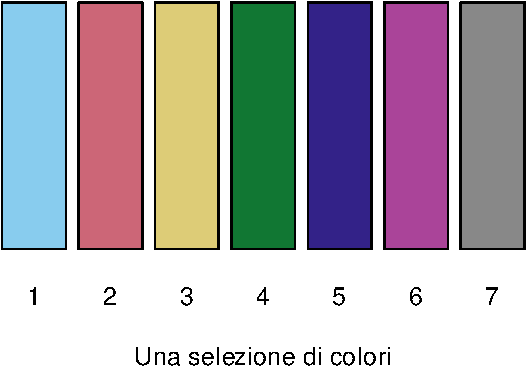
\includegraphics[keepaspectratio]{index_files/figure-pdf/colori-1.pdf}}
\end{center}

\end{remark}

Ogni sezione include alla fine un paio di esercizi (di solito varianti
degli esempi visti nel testo) che si suggerisce di provare svolgere in
autonomia, senza rinunciare all'ausilio di opportuno codice R. Ogni
capitolo contiene inoltre una sezione conclusiva di problemi da
svolgere, analoghi a quelli della prova scritta dell'esame. Si consiglia
di risolverli sia analiticamente che numericamente tramite opportuni
comandi R.

Sicuramente questi appunti, come pure il corso stesso, possono essere
migliorati: sono sempre disponibile ad ascoltare le vostre osservazioni,
i suggerimenti e le eventuali critiche. Inoltre sono purtroppo
consapevole che gli errori tipografici in queste pagine abbondano, e
invito tutte e tutti a segnalarli via e-mail in modo che possa
correggerli tempestivamente\footnote{Ringrazio gli studenti Matteo Di
  Pietro, Francesco Paolo Carmone, Matteo Mariani per le segnalazioni.}.

\bookmarksetup{startatroot}

\chapter{Probabilità elementare}\label{sec-intro-prob}

In questo capitolo introduciamo la probabilità come calcolo del grado di
fiducia circa la validità di una affermazione, sulla base di
informazione parziale.

\begin{itemize}
\item
  Nella Sezione~\ref{sec-intuitivo}, introduciamo il concetto intuitivo
  di probabilità dal punto di vista \textbf{soggettivo}.
\item
  Nella Sezione~\ref{sec-somma} affrontiamo la prima regola di calcolo
  fondamentale (\textbf{regola della somma}, o additività) e alcune
  semplici conseguenze.
\item
  Nella Sezione~\ref{sec-alternative} introduciamo il concetto
  fondamentale di \textbf{sistema di alternative} (finito) e di densità
  discreta ad esso associata.
\item
  Nella Sezione~\ref{sec-prodotto} presentiamo la seconda regola di
  calcolo fondamentale (\textbf{regola del prodotto} o della probabilità
  composta) e alcune conseguenze.
\item
  La Sezione~\ref{sec-alberi} si occupa dell'analisi di problemi
  probabilistici elementari tramite \textbf{diagrammi ad albero}. Si
  introduce in particolare il modello delle estrazioni da un'urna (senza
  rimpiazzo).
\item
  La breve, ma importantissima, Sezione~\ref{sec-bayes} è dedicata la
  deduzione della \textbf{formula di Bayes}, uno degli strumenti chiave
  del calcolo delle probabilità.
\item
  La Sezione~\ref{sec-bayes-stat} mostra come la formula di Bayes
  fornisca un metodo generale (detto appunto Bayesiano) per approcciare
  semplici problemi di inferenza statistica, in particolare per stimare
  la plausibilità di un'ipotesi sulla base di dati osservati.
  Introduciamo anche il metodo di \textbf{massima verosimiglianza}, come
  semplice ma spesso efficace stima dell'ipotesi più probabile.
\item
  Nella Sezione~\ref{sec-indipendenza} definiamo l'\textbf{indipendenza
  probabilistica} tra due o più eventi: per esperienza, questo concetto
  è particolarmente insidioso e quindi viene presentato e discusso in
  modo dettagliato, accompagnandolo con il modello delle estrazioni da
  un'urna (con rimpiazzo).
\item
  Nella Sezione~\ref{sec-assiomi}, accenniamo alla
  \textbf{formalizzazione assiomatica} della probabilità proposta da
  Kolmogorov, estremamente importante per la dimostrazione di risultati
  teorici, in particolare teoremi limite, ma sicuramente meno per i fini
  modellistico-computazionali.
\end{itemize}

\section{Cos'è la probabilità?}\label{sec-intuitivo}

Mentre le regole di calcolo della probabilità sono universalmente
accettate e usate in vari ambiti scientifici, vi sono diverse scuole di
pensiero relative all'interpretazione della probabilità stessa e delle
sue applicazioni. Senza entrare nei dettagli della questione, in questo
corso adottiamo un'interpretazione \textbf{soggettiva} perché ci
permetterà di ottenere risultati applicabili in contesti più vari
(rispetto all'intepretazione frequentista).

\begin{quote}
La probabilità misura \textbf{il grado di fiducia} che un soggetto
attribuisce alla \textbf{validità di una affermazione}, avendo a
disposizione una \textbf{informazione parziale} (che in generale non
permette di dedurre la verità o la falsità dell'affermazione).
\end{quote}

Teniamo presente che, quando consideriamo un soggetto e il grado di
fiducia che attribuisce ad un'affermazione, non siamo in realtà
interessati ad una persona o ad un gruppo di persone specifiche (sarebbe
piuttosto campo di indagine della psicologia o della sociologia), quanto
piuttosto ad una idealizzazione di una \textbf{intelligenza razionale},
come potrebbe essere un essere umano (de-)privato di tutte le emozioni,
gli istinti, ecc. Si tratta dello stesso procedimento che interviene
nello studio della logica matematica, come astrazione del ragionamento
deduttivo. Come per la logica, i risultati che si ottengono tramite il
calcolo delle probabilità sono ovviamente utili anche per lo studio di
problemi reali, che possono riguardare intelligenze umane o artificiali.

\begin{remark}
Una delle difficoltà dovute all'intepretazione soggettiva della
probabilità, anche nello svolgimento degli esercizi, è proprio nel
mantenere un grado di separazione con il soggetto astratto cui è
richiesto di determinare una probabilità sulla base di una certa
informazione. La nostra intuizione, allenata dal buon senso e
dall'esperienza, in molti casi ci suggerisce una risposta senza però
fornirci un percorso per giustificarla completamente. Il calcolo delle
probabilità diventa quindi un modo per \emph{programmare} il soggetto
razionale a risolvere dei problemi -- anche se noi stessi in certi casi
ne sappiamo intuitivamente già dare una soluzione. Per aiutarci in
questa separazione di ruoli, conveniamo in questo corso di introdurre un
personaggio fittizio, corrispondente a questo soggetto razionale del
tutto ideale, che chiameremo \textbf{il robot}, come nella monografia di
E.T. Jaynes,
\href{https://www.cambridge.org/core/books/probability-theory/9CA08E224FF30123304E6D8935CF1A99}{\emph{Probability
Theory The Logic of Science}}, un testo consigliato per chi voglia
approfondire gli aspetti del calcolo delle probabilità come logica
dell'incertezza.
\end{remark}

Date queste premesse, il calcolo della probabilità può essere quindi
posto come il seguente \textbf{problema generale}, che affronteremo in
tutto questro corso in molteplici contesti particolari: assegnate al
robot

\begin{enumerate}
\def\labelenumi{\arabic{enumi}.}
\tightlist
\item
  una \textbf{informazione}, che indichiamo con \(I\), \textbf{nota} e
  ritenuta vera (dal robot),
\item
  una \textbf{affermazione}, che indichiamo con \(A\), che nella realtà
  può essere solo vera oppure falsa (senza ambiguità),
\end{enumerate}

è richiesto al robot di misurare il grado di incertezza circa la
validità di \(A\), sulla base di tutta e sola l'informazione \(I\), nel
modo più razionale possibile.

Tale misura, detta la \textbf{probabilità di} \(A\) sapendo \(I\) (o
nota \(I\), o anche condizionata ad \(I\)) deve essere un numero reale
compreso tra \(0\) e \(1\), e si indica con la notazione \[ P(A | I).\]

Sicuramente avrete incontrato esempi di probabilità associate a
\emph{giochi} come lanci di dadi, monete, oppure estrazioni di carte.
Queste applicazioni storicamente motivarono i primi studi sulla
probabilità, ma pensare alla probabilità solo in questi termini al
giorno d'oggi è estremamente riduttivo. Ecco due esempi di problemi
reali in cui il calcolo delle probabilità fornisce degli strumenti molto
importanti (ovviamente poi non è l'unico ingrediente per la loro
risoluzione).

Potremmo chiedere al robot di valutare se ``oggi pioverà a Pisa''
(affermazione \(A\)) sapendo che ``oggi è nuvoloso'' (informazione nota
\(I\)). Le previsioni meteorologiche ovviamente non si basano sulla
banale informazione \(I\) sopra, bensì sul numerosissime misurazioni di
quantità fisiche e calcoli numerici su specifici modelli. Il calcolo
delle probabilità gioca un ruolo importante per quantificare
l'incertezza associata al risultato (la previsione) fornito.

Data una immagine (informazione nota \(I\)), potremmo chiedere al robot
di valutare se essa ``rappresenti un volto umano'' (\(A\)). Questo è un
problema che noi esseri umani risolviamo in pochissimo tempo
(appoggiandoci sulla lunga storia della nostra evoluzione). Dare una
risposta automatizzata a questo e simili questioni di classificazione,
pochi anni fa era considerato fantascienza, mentre oggi è un compito
alla portata di uno smartphone. Tra vari aspetti che hanno permesso
questo sviluppo, un punto di svolta è stata l'introduzione di opportuni
modelli matematici, anche basati sul calcolo delle probabilità, in modo
da ``insegnare'' al robot come rispondere sulla base dell'informazione
contenuta in grandissime raccolte di immagini classificate (un po' come
nei modelli metereologici, la vera informazione nota \(I\) è quindi
molto di più della singola immagine fornita al robot).

In questo corso ovviamente non ci occuperemo di problemi così specifici
e gli esempi che tratteremo saranno forse meno affascinanti. Lo scopo
però è di fornire un linguaggio e gli strumenti matematici opportuni
anche per avvicinarsi a queste ed altre questioni, estremamente
rilevanti ai fini pratici.

Introduciamo ora alcuni termini tecnici propri del calcolo delle
probabilità.

Se \(P(A|I) = 1\), significa che \(A\) è ritenuta dal robot praticamente
vera (si dice tecnicamente \textbf{quasi certa}), mentre se
\(P(A|I) = 0\), significa l'opposto, ossia ritenuta praticamente falsa,
e si dice allora che \(A\) è \textbf{trascurabile} (condizionatamente ad
\(I\)).

Si usa il termine generico \textbf{evento} per indicare le affermazioni
che si considerano nel calcolo, come \(A\) o anche l'informazione nota
\(I\) (che pure possiamo pensare come un'affermazione). Si usa dire
anche che l'evento \(A\) \textbf{si realizza} per affermare che \(A\) è
vero. Questo perché storicamente il calcolo della probabilità riguardava
affermazioni su fatti legati al gioco d'azzardo, come ad esempio il
lancio di un dado o l'estrazione del lotto. Anche noi useremo questo
termine, ma spesso accompagnandolo con sinonimi meno tecnici e in certi
casi più evocativi, come affermazione o informazione.

Le operazioni logiche elementari tra affermazioni saranno usate di
continuo e adotteremo varie notazioni.

\begin{enumerate}
\def\labelenumi{\arabic{enumi}.}
\item
  Per indicare la \textbf{negazione} di una affermazione \(A\), ossia
  l'affermazione che è vera se e solo se \(A\) è falsa, scriveremo ``non
  \(A\)'' oppure la notazione insiemistica per il \emph{complementare}
  \(A^c\).
\item
  Per la \textbf{congiunzione logica} tra \(A\) e \(B\), ossia
  l'affermazione che è vera se e solo se \(A\), \(B\) sono entrambe
  vere, scriviamo ``\(A\) e \(B\)'' oppure semplicemente \(A,B\) (con la
  virgola) oppure la notazione insiemistica per l'\emph{intersezione}
  \(A\cap B\).
\item
  Infine, per la \textbf{disgiunzione} (inclusiva) tra \(A\) e \(B\),
  ossia l'affermazione che è vera se e solo se almeno una tra \(A\),
  \(B\) è vera, scriviamo ``\(A\) oppure \(B\)'', ``\(A\) o \(B\)'', o
  useremo la notazione insiemistica per l'\emph{unione} \(A \cup B\).
\end{enumerate}

Sempre a proposito di notazione, per alleggerire formule altrimenti
pesanti, spesso l'informazione nota al robot (che abbiamo indicato con
\(I\), ma ovviamente può cambiare) è sottointesa, specialmente se non ci
sono ambiguità, e scriveremo solamente
\[ P(A) \quad \text{ al posto di } \quad  P(A|I).\]

\begin{remark}
Questa notazione semplificata tuttavia non deve trarre in inganno:
\textbf{tutte le probabilità sono sempre condizionate} ad una
informazione nota \(I\), magari anche estremamente banale. Il suo ruolo
è analogo a quello delle ipotesi in un teorema, mentre quello di \(A\) è
simile a quello della tesi, quindi entrambi fondamentali! Spesso negli
esercizi di probabilità si sottovaluta o misintepreta l'informazione
presentata nel testo (che va a definire l'informazione \(I\)), facendo
di fatto calcolare al robot delle probabilità diverse da quelle
richieste.
\end{remark}

Il nostro obiettivo, nelle prossime sezioni, sarà di introdurre delle
regole di calcolo per la probabilità, in un certo senso analoghe a
quelle della logica, ma diverse e, come vedremo, più flessibili.
Ridurremo tutto a due regole fondamentali, dette brevemente della
\textbf{somma} e del \textbf{prodotto}. Non ci occuperemo troppo di
giustificarle, quanto piuttosto di mostrare come da esse seguano le
altre regole utili che permettono di calcolare probabilità per risolvere
problemi (anche se elementari) in modo efficace.

Prima di vedere tali regole, osserviamo le seguente proprietà di
monotonia della probabilità, semplice ma a volte sfuggevole\footnote{si
  veda l'esempio della
  \href{http://maddmaths.simai.eu/divulgazione/fallacia-della-congiunzione/}{fallacia
  della congiunzione}.}.

Date due affermazioni \(A\) e \(B\) e l'informazione nota \(I\), se
\(A\) è vera in qualsiasi situazione in cui \(B\) sia vera (supponendo
sempre vera \(I\)), allora vale \[ P(B | I ) \le P(A | I ).\]

Alternativamente, la condizione ``\(A\) è vera ogni volta che \(B\) lo
è'' si può formulare come ``l'implicazione logica \(B \to A\) è vera''
(supponendo vera \(I\)). Il caso più semplice è quando \(B\) sia
ottenuta come la congiunzione di \(A\) e un'altra affermazione, ad
esempio \(A\) è ``oggi piove'', \(B\) è ``oggi piove e porto
l'ombrello''.

\begin{remark}
Per visualizzare la proprietà di monotonia e le successive regole di
calcolo, introduciamo la rappresentazione grafica a \textbf{diagrammi di
Eulero-Venn} degli eventi, ossia delle affermazioni e dell'informazione
nota. Precisamente, possiamo pensare l'informazione nota al robot \(I\)
come un \emph{universo}, rappresentato tramite un riquadro, in cui tutte
le altre affermazioni sono contenute. Tradizionalmente, i diagrammi
rappresentano insiemi, mentre in questo caso sono affermazioni: sarà
sufficiente pensare agli ipotetici \emph{elementi} contenuti in questi
diagrammi come alle possibili situazioni in cui l'affermazione è vera
(in termini probabilistici, l'evento si realizza). Questo è in linea con
la descrizione assiomatica di Kolmogorov, cui si accenna nella
Sezione~\ref{sec-assiomi}. Comunque, eccetto per problemi estremamente
semplici, i diagrammi di Eulero-Venn non sono molto pratici, e li
abbandoneremo presto per rappresentazioni più utili, come i diagrammi ad
albero e le reti bayesiane.

\begin{figure}[H]

{\centering \pandocbounded{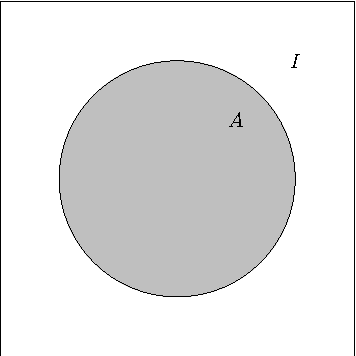
\includegraphics[keepaspectratio]{eventi_files/figure-pdf/unnamed-chunk-2-1.pdf}}

}

\caption{Diagramma rappresentante l'informazione nota \(I\) e un evento
\(A\).}

\end{figure}%

Qualitativamente, la probabilità di \(A\) è associata all'\textbf{area}
del suo diagramma: tanto più esteso, maggiore sarà la sua probabilità,
fino al caso in cui \(A\) copra tutto l'universo \(I\), ossia \(A\) è
quasi certo, \(P(A|I)=1\). D'altra parte, se \(A\) è trascurabile,
\(P(A|I)=0\), possiamo rappresentare \(A\) così piccolo da evitare del
tutto di disegnarlo -- precisamente il diagramma \emph{vuoto}
corrisponde ad una affermazione trascurabile, sapendo \(I\).

Le operazioni logiche di congiunzione (\emph{e}) e disgiunzione
inclusiva (\emph{oppure}) corrispondono rispettivamente all'intersezione
e all'unione tra i diagrammi. La negazione (\emph{non}) corrisponde al
complementare (relativamente all'universo \(I\)), mentre la condizione
che implica la monotonia della probabilità, ossia ``\(A\) è vera ogni
volta che \(B\) lo è'' corrisponde all'inclusione tra i diagrammi.

\begin{figure}[H]

{\centering \pandocbounded{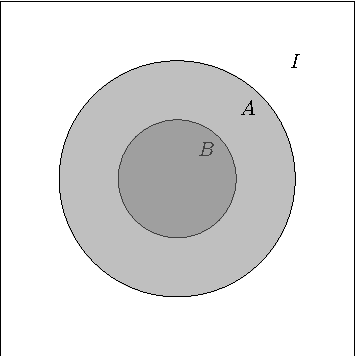
\includegraphics[keepaspectratio]{eventi_files/figure-pdf/unnamed-chunk-3-1.pdf}}

}

\caption{\(A\) è vera ogni volta che \(B\) lo è, ossia l'implicazione
\(B \to A\) è vera.}

\end{figure}%

\end{remark}

\subsection{Esercizi}\label{esercizi}

Disegnare il diagramma di Venn associato all'affermazione ``non (\(A\) e
\(B\))'' e verificare che coincide con quello di ``(non \(A\)) o (non
\(B\))'' (regola di De Morgan).

Fornire un esempio concreto di affermazioni \(A\), \(B\) ed \(I\) in cui
è intuitivamente chiaro che \(P(A|I) \le P(A|I\cap B)\) e uno in cui
all'opposto \(P(A|I) \ge P(A|I \cap B)\).

\section{Regola della somma}\label{sec-somma}

La prima regola del calcolo delle probabilità riguarda la disgiunzione
logica tra due affermazioni.

Date affermazioni \(A\), \(B\) e l'informazione nota \(I\), se \(A\) e
\(B\) non possono in nessun caso essere entrambe vere (supponendo \(I\)
vera), allora vale
\[ P( A \text{ oppure } B | I ) = P(A | I )+ P(B|I). \]

Due affermazioni \(A\) e \(B\) come sopra vengono dette
\textbf{incompatibili} (o mutuamente esclusive), proprio perché la
validità di una esclude l'altra. Equivalentemente, possiamo anche dire
che l'affermazione ``\(A\) e \(B\)'' è trascurabile rispetto
all'informazione \(I\), ossia \(P( A,B | I ) = 0\). Con la
rappresentazione in diagrammi, notiamo che la condizione di
incompatibilità corrisponde al fatto che i diagrammi siano ben separati
(il termine insemistico è \textbf{disgiunti}), e la regola della somma
corrisponde al fatto che l'area dell'unione dei diagrammi sia la somma
delle aree.

\begin{figure}[H]

{\centering \pandocbounded{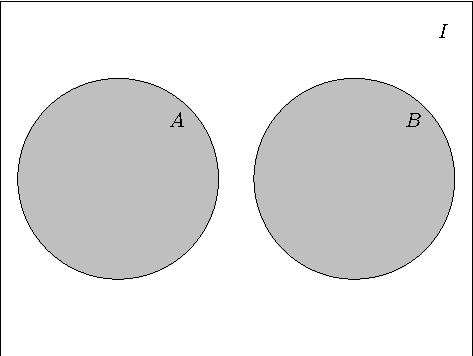
\includegraphics[keepaspectratio]{eventi_files/figure-pdf/unnamed-chunk-4-1.pdf}}

}

\caption{Regola della somma tra \(A\) e \(B\) incompatibili.}

\end{figure}%

L'esempio più semplice di eventi incompatibili si ottiene ponendo \(B\)
come la negazione di \(A\) ossia \(B=\) ``non \(A\)''. Siccome ``\(A\)
oppure \(B\)'' è così sicuramente vera (qualsiasi sia l'informazione
\(I\), che quindi omettiamo), ne deduciamo che
\[ 1 = P( \text{ $A$ oppure non $A$}  ) = P(A)+ P(\text{non $A$}),\]
ossia \[ P(\text{non $A$}) = 1 - P(A).\]

Nel caso di affermazioni \(A\), \(B\) non incompatibili, si ottiene una
formula leggermente più complicata, a volte utile.

Per \(A\) e \(B\) affermazioni (non necessariamente incompatibili) vale
\begin{equation}\protect\phantomsection\label{eq-sum-general}{
P(\text{$A$ oppure $B$}  ) = P(A  )+ P(B)  - P(\text{$A$ e $B$} ),
}\end{equation} dove per brevità omettiamo di specificare l'informazione
nota \(I\).

\begin{figure}[H]

{\centering \pandocbounded{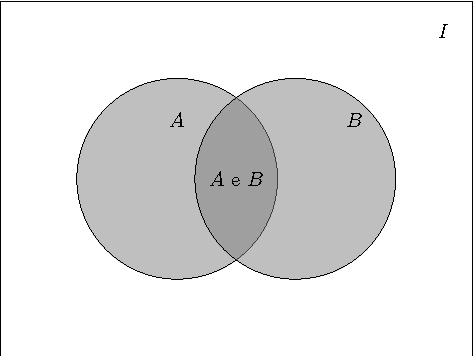
\includegraphics[keepaspectratio]{eventi_files/figure-pdf/unnamed-chunk-5-1.pdf}}

}

\caption{Regola della somma tra \(A\) e \(B\) generali: l'area
dell'intersezione va sottratta altrimenti è contata due volte.}

\end{figure}%

\begin{proof}
Infatti, l'affermazione ``\(A\) oppure \(B\)'' si può equivalentemente
pensare come ``\(A\) oppure (\(B\) e non \(A\))'', nel senso che una è
vera se e solo se l'altra è vera: perciò il grado di fiducia attribuito
deve essere lo stesso (altrimenti il robot non sarebbe davvero
razionale). Ma nella riformulazione, le due affermazioni \(A\) e ``\(B\)
e non \(A\)'' sono incompatibili. Ne segue che
\[ P(\text{$A$ oppure $B$} ) = P(A) + P(\text{$B$ e non $A$}).\]
Analogamente, scambiando i ruoli di \(A\) e \(B\) segue che
\[ P(B) = P(\text{$B$ e $A$}) + P(\text{$B$ e non $A$}),\] e sottraendo
le due identità otteniamo la Equazione~\ref{eq-sum-general}.
\end{proof}

\subsection{Esercizi}\label{esercizi-1}

Mostrare la seguente regola della somma generalizzata a tre eventi
\(A\), \(B\), \(C\) qualsiasi (non necessariamente incompatibili):
\[ P( \text{$A$ oppure $B$ oppure $C$}) = P(A)+P(B)+P(C) - P(A,B)-P(A,C)-P(B,C) + P(A,B,C).\]

Dedurre la proprietà di monotonia dalla regola della somma.

\section{Sistemi di alternative}\label{sec-alternative}

Una ulteriore conseguenza della regola della somma riguarda l'estensione
al caso di \(n\) affermazioni \(A_1\), \(A_2\), \ldots, \(A_n\). Diciamo
che esse sono \textbf{a due a due incompatibili} tra loro se per
ciascuna coppia \(A_i\), \(A_j\) con \(i \neq j\), esse sono
incompatibili, ossia ``\(A_i\) e \(A_j\)'' è trascurabile (rispetto
all'informazione nota \(I\)). Ragionando sulla regola della somma e
usando l'induzione matematica, si ottiene che per l'affermazione
``almeno una tra le \(A_i\) è vera'', ossia ``\(A_1\) oppure \(A_2\)
oppure \ldots{} \(A_n\)'', vale
\[P( \text{almeno una tra le $A_i$ è vera} | I) =  P(A_1|I)+ \ldots + P(A_n|I) = \sum_{i=1}^n P(A_i|I).\]

\begin{example}[]\protect\hypertarget{exm-dado}{}\label{exm-dado}

Si consideri il lancio di un dado a sei facce e per ogni
\(i \in \cur{1, \ldots, 6}\), si ponga \(A_i\) l'affermazione ``esce la
faccia \(i\)''. Allora vale
\[ P( \text{esce una faccia pari}) = P(\text{una tra $A_2$, $A_4$ o $A_6$ è vera}) = P(A_2)+P(A_4)+P(A_6).\]

\end{example}

Date affermazioni \(A_i\) a due a due incompatibili, non necessariamente
una di esse deve essere sempre vera, ma se questo è il caso (come
nell'esempio sopra per \(i=\cur{1,2,3,4,5,6}\)) allora \textbf{una e una
sola} tra le \(A_i\) è necessariamente vera (ma spesso il robot di
solito non sa quale sia). Ne segue che
\[1 = P( \text{una tra le $A_i$ è vera} ) = \sum_{i=1}^n P(A_i).\] In
questa situazione, le \((A_i)_{i=1}^n\) sono dette un \textbf{sistema di
alternative}.

Un \textbf{sistema di alternative} (rispetto ad una informazione \(I\))
è una famiglia \((A_i)_{i=1}^n\) di affermazioni (dette alternative)

\begin{enumerate}
\def\labelenumi{\arabic{enumi}.}
\tightlist
\item
  a due a due incompatibili (o mutuamente esclusive) e
\item
  tali che almeno una tra loro è sicuramente vera.
\end{enumerate}

In breve, \textbf{una e una sola} tra le alternative è sicuramente vera
(nota \(I\)).

\begin{remark}
In questo capitolo ci limiteremo a sistemi con un numero \(n\) finito di
alternative. In seguito, considereremo sistemi infiniti, ma useremo un
linguaggio più adatto a trattarli, quello delle variabili aleatorie.
\end{remark}

Ad un'affermazione \(A\), si può sempre associare il sistema di
alternative costituito da \(A\) e la sua negazione ``non \(A\)''.

Rappresentato in diagrammi, un sistema di alternative corrisponde ad una
\textbf{partizione} dell'universo \(I\).

\begin{figure}[H]

{\centering \pandocbounded{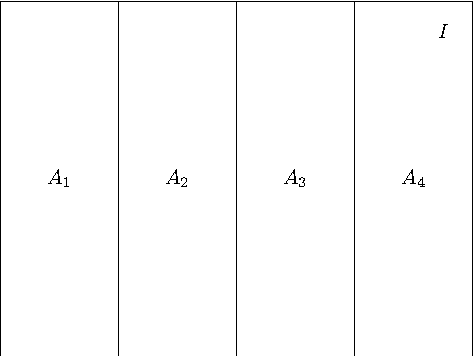
\includegraphics[keepaspectratio]{eventi_files/figure-pdf/unnamed-chunk-6-1.pdf}}

}

\caption{Rappresentazione di un sistema di \(4\) alternative.}

\end{figure}%

I sistemi di alternative sono uno degli strumenti fondamentali per
risolvere i problemi elementari di probabilità, in particolare per
decomporre (\emph{analizzare}) un problema complesso in una famiglia di
sotto-problemi più semplici da trattare. Vale infatti la seguente
generalizzazione della regola della somma (la cui deduzione è lasciata
per esercizio).

Sia \((A_i)_{i=1}^n\) un sistema di alternative (rispetto
all'informazione \(I\)) e sia \(B\) una (qualsiasi) affermazione. Allora
si può decomporre
\[ P(B|I) = P(\text{$B$ e $A_1$}|I)+ \ldots + P(\text{$B$ e $A_n$}|I).\]

\begin{figure}[H]

{\centering \pandocbounded{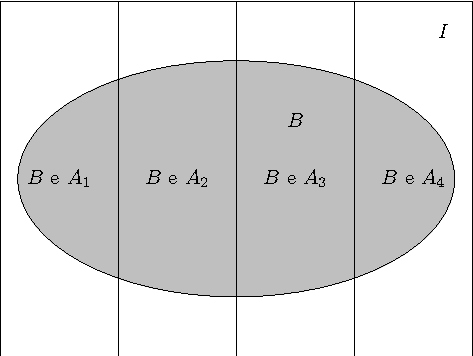
\includegraphics[keepaspectratio]{eventi_files/figure-pdf/unnamed-chunk-7-1.pdf}}

}

\caption{Rappresentazione della formula di decomposizione.}

\end{figure}%

\subsection{Densità discreta}\label{densituxe0-discreta}

Ad un sistema di alternative \((A_i)_{i=1}^n\) (rispetto
all'informazione \(I\)) possiamo associare la collezione delle
probabilità \[ \bra{P(A_i|I)}_{i=1}^n.\] Come conseguenza della regola
della somma, ciascuna \(p_i := P(A_i|I)\) è un numero compreso tra \(0\)
ed \(1\) ed inoltre vale \[ \sum_{i=1}^n p_i = 1.\] Una tale famiglia di
numeri è detta \textbf{densità discreta} di probabilità. A ogni sistema
di alternative è quindi associata una densità discreta (rispetto ad una
informazione nota \(I\)).

Data una qualsiasi funzione \(i \mapsto f(i)\), definita per
\(i\in\cur{1, \ldots, n}\), a valori non-negativi (e non identicamente
nulla), si può associare una e una sola densità discreta proporzionale
ad \(f\), ossia tale che
\[ p_i = c f(i) \quad \text{per ogni $i \in \cur{1, \ldots, n}$,}\] per
una costante moltiplicativa \(c>0\) (che non dipenda da \(i\)).
Imponendo infatti che la somma delle \(p_i\) sia uno, si trova il valore
\[c = \bra{ \sum_{i=1}^n f(i)}^{-1}.\] Sfruttando questo fatto, è molto
comodo spesso definire una densità discreta a meno di costante
moltiplicativa, e si scrive di solito \[ p_i \propto f(i),\] (si legge
``\(p_i\) è proporzionale ad \(f(i)\)'').

Alcune densità discrete si presentano più frequentemente di altre, e
sono state storicamente classificate, spesso attribuendo ad esse il nome
di chi le ha studiate per primo, o più a fondo (purtroppo tale scelta ne
rende un po' difficile e noiosa la memorizzazione). Introduciamo due
esempi fondamentali, altre verranno discusse in seguito.

Supponendo di avere \(n\) alternative \((A_i)_{i=1}^n\), la densità
uniforme è il caso in cui tutte le probabilità siano uguali tra loro,
ossia \[ P(A_i|I) = \frac 1 n,\] o, più semplicemente,
\[ P(A_i|I) \propto 1.\] Questa densità discreta è usata quando non vi
siano ragioni, data l'informazione \(I\), per distinguere (o
``preferire'') una alternativa \(A_i\) rispetto alle altre (questo è il
\emph{principio di indifferenza di Laplace}). È una densità discreta che
si introduce spesso per iniziare lo studio di un problema, di cui si
conoscono pochi aspetti. Ad esempio, nel caso del lancio di un dado a
sei facce, prima del lancio, non sapendo alcunché sul dado o su come si
effutta il lancio, il robot per il principio di Laplace supporrà che la
densità delle sei alternative \(A_i\) indicate nell'Esempio @exm:dado
sia uniforme.

\begin{Shaded}
\begin{Highlighting}[]
\CommentTok{\# Costruiamo un vettore costante con la funzione rep() e poi dividiamo opportunamente perché la somma sia uno, usando la funzione sum(). Il passaggio in questo caso  è banale ma sarà utile in altre occasioni.}

\NormalTok{n }\OtherTok{\textless{}{-}} \DecValTok{6}
\NormalTok{dens\_uniforme }\OtherTok{\textless{}{-}} \FunctionTok{rep}\NormalTok{(}\DecValTok{1}\NormalTok{,n)}
\NormalTok{dens\_uniforme }\OtherTok{\textless{}{-}}\NormalTok{ dens\_uniforme}\SpecialCharTok{/}\FunctionTok{sum}\NormalTok{(dens\_uniforme)}

\CommentTok{\# Introduciamo dei parametri per il plot, come le etichette  da inserire sotto le barre e il colore (grigio)}

\NormalTok{alternative }\OtherTok{=} \FunctionTok{as.character}\NormalTok{(}\DecValTok{1}\SpecialCharTok{:}\DecValTok{6}\NormalTok{)}

\CommentTok{\# Usiamo il comando barplot() per produrre il grafico}

\FunctionTok{barplot}\NormalTok{( dens\_uniforme, }\AttributeTok{col=}\NormalTok{miei\_colori[}\DecValTok{1}\NormalTok{], }\AttributeTok{names.arg=}\NormalTok{alternative, }\AttributeTok{ylab=}\StringTok{"probabilità"}\NormalTok{, }\AttributeTok{xlab=}\StringTok{"alternativa"}\NormalTok{)}
\end{Highlighting}
\end{Shaded}

\begin{figure}[H]

{\centering \pandocbounded{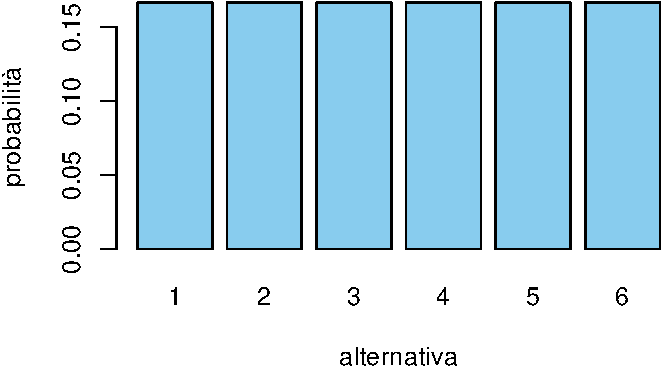
\includegraphics[keepaspectratio]{eventi_files/figure-pdf/unnamed-chunk-8-1.pdf}}

}

\caption{Grafico a barre della densità discreta uniforme su \(n = 6\)
alternative.}

\end{figure}%

Questa è sicuramente la densità discreta più semplice -- ma ha un nome
complicato da ricordare! È la densità associata ad un qualsiasi sistema
di due sole alternative, ossia \(A_1\) e la sua negazione ``non
\(A_1\)'', che si indica tradizionalmente questo caso con \(A_0\). È
sufficiente indicare quindi il valore di una sola probabilità,
\(p := P(A_1|I)\), poiché di conseguenza \(P(A_0|I) =1 -p\). Il valore
\(p \in [0,1]\) è detto \textbf{parametro} della densità Bernoulli.
Molte di queste densità notevoli presentano in effetti naturalmente dei
parametri (numeri naturali, reali ecc.) che vanno precisati per
determinarle completamente -- stiamo quindi precisamente descrivendo una
famiglia di densità discrete, ciascuna identificata qui dal valore del
parametro \(p\).

\begin{Shaded}
\begin{Highlighting}[]
\CommentTok{\# Ricordiamo che che il parametro p indica la probabilità dell\textquotesingle{}alternativa 1 (l\textquotesingle{}altra invece indicata con 0)}

\NormalTok{dens\_bernoulli\_1\_3 }\OtherTok{\textless{}{-}} \FunctionTok{c}\NormalTok{(}\DecValTok{2}\SpecialCharTok{/}\DecValTok{3}\NormalTok{, }\DecValTok{1}\SpecialCharTok{/}\DecValTok{3}\NormalTok{)}
\NormalTok{dens\_bernoulli\_1\_2 }\OtherTok{\textless{}{-}} \FunctionTok{c}\NormalTok{(}\DecValTok{1}\SpecialCharTok{/}\DecValTok{2}\NormalTok{, }\DecValTok{1}\SpecialCharTok{/}\DecValTok{2}\NormalTok{)}
\NormalTok{dens\_bernoulli\_2\_3 }\OtherTok{\textless{}{-}} \FunctionTok{c}\NormalTok{(}\DecValTok{1}\SpecialCharTok{/}\DecValTok{3}\NormalTok{, }\DecValTok{2}\SpecialCharTok{/}\DecValTok{3}\NormalTok{)}

\CommentTok{\# per fare un singolo grafico costruiamo una matrice a partire dalle densità (ciascuna densità è una riga)}

\NormalTok{dens\_bernoulli\_matrice }\OtherTok{\textless{}{-}} \FunctionTok{matrix}\NormalTok{( }\FunctionTok{c}\NormalTok{(dens\_bernoulli\_1\_3, dens\_bernoulli\_1\_2, dens\_bernoulli\_2\_3), }\AttributeTok{nrow=}\DecValTok{3}\NormalTok{, }\AttributeTok{byrow=}\ConstantTok{TRUE}\NormalTok{)}

\CommentTok{\# Plottiamo il diagramma a barre}

\NormalTok{alternative }\OtherTok{=} \FunctionTok{c}\NormalTok{(}\StringTok{"0"}\NormalTok{, }\StringTok{"1"}\NormalTok{)}
\NormalTok{colori }\OtherTok{=}\NormalTok{ miei\_colori[}\DecValTok{1}\SpecialCharTok{:}\DecValTok{3}\NormalTok{]}

\FunctionTok{barplot}\NormalTok{( dens\_bernoulli\_matrice, }\AttributeTok{beside=}\ConstantTok{TRUE}\NormalTok{, }\AttributeTok{col=}\NormalTok{colori, }\AttributeTok{names.arg=}\NormalTok{alternative, }\AttributeTok{ylab=}\StringTok{"probabilità"}\NormalTok{, }\AttributeTok{xlab=}\StringTok{"alternativa"}\NormalTok{)}

\CommentTok{\# Aggiungiamo una legenda}

\FunctionTok{legend}\NormalTok{(}\StringTok{\textquotesingle{}top\textquotesingle{}}\NormalTok{, }\AttributeTok{fill=}\NormalTok{colori, }\AttributeTok{legend=}\FunctionTok{c}\NormalTok{(}\StringTok{"p=1/3"}\NormalTok{, }\StringTok{"p=1/2"}\NormalTok{, }\StringTok{"p=2/3"}\NormalTok{), }\AttributeTok{cex=}\FloatTok{0.8}\NormalTok{)}
\end{Highlighting}
\end{Shaded}

\begin{figure}[H]

{\centering \pandocbounded{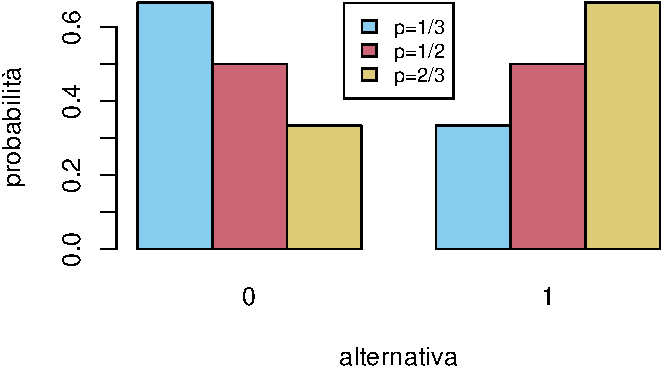
\includegraphics[keepaspectratio]{eventi_files/figure-pdf/unnamed-chunk-9-1.pdf}}

}

\caption{Grafico a barre della densità Bernoulli di parametri \(p=1/3\),
\(p=1/2\) e \(p=2/3\).}

\end{figure}%

Dato un sistema di alternative \((A_i)_{i=1}^n\), una domanda naturale è
di individuare quale sia la più plausibile, sulla base dell'informazione
nota \(I\). Si tratta pertanto determinare \(i_{\max}\) tale che
\[ P(A_{i_{\max}} |I ) = \max_{i=1, \ldots, n} P(A_{i} |I ),\] ossia
\[ i_{\max} \in \operatorname{arg} \max \cur{ P(A_i|I) : i \in \cur{1, \ldots, n}}.\]
Nella statistica tale \(i_{\max}\) è detto \textbf{moda} della densità
discreta (notiamo che non è necessariamente unica, si pensi al caso di
una densità uniforme).

\begin{remark}
Spesso, per determinare la moda \(i_{\max}\) conviene passare al
logaritmo (che essendo una funzione crescente, non cambia il problema) e
determinare
\[ i_{\max} \in \operatorname{arg} \max \cur{ \log(  P(A_i|I) ): i \in \cur{1, \ldots, n}}.\]
Se invece si preferisce \emph{minimizzare} una funzione invece di
massimizzarla (molti metodi numerici sono naturalmente implementati per
trovare il minimo, non il massimo di una funzione), ovviamente basta
cambiare di segno:
\[ i_{\max} \in \operatorname{arg} \min \cur{ -\log(  P(A_i|I) ): i \in \cur{1, \ldots, n}}.\]
\end{remark}

\subsection{Esercizi}\label{esercizi-2}

Si consideri la densità discreta \[ p_i \propto i^2 \] per
\(i \in \cur{1, \ldots, 10}\). Determinare la costante moltiplicativa e
rappresentare la densità tramite un grafico a barre. Calcolarne la moda
\(i_{\max}\) e dire se è unica.

Si consideri la densità discreta \[ p_i \propto i^2(5-i)^4\] per
\(i \in \cur{1, 2, \ldots, 5}\). Determinare la costante moltiplicativa
e rappresentare la densità tramite un grafico a barre. Calcolarne la
moda \(i_{\max}\) e dire se è unica.

\section{Regola del prodotto}\label{sec-prodotto}

Passiamo ora alla seconda regola di calcolo, che afferma, nel caso della
congiunzione tra due affermazioni, come la probabilità si ottenga
tramite un opportuno prodotto.

Date affermazioni \(A\), \(B\) e l'informazione nota \(I\), vale
\[ P( A \text{ e } B | I ) = P( A | I )P(B | A, I). \]

L'interpretazione di questa formula è la seguente: dovendo attribuire il
grado di fiducia che entrambe \(A\) e \(B\) siano vere, il robot può
calcolare prima la probabilità che \(A\) sia vera e poi, supponendo che
anche \(A\) sia vera (e quindi la si aggiunge all'informazione nota
\(I\)), calcola la probabilità che sia vera \(B\), e infine moltiplica i
due risultati.

Sottointendendo l'informazione \(I\), si trova la scrittura più agevole
\[ P( A \text{ e } B  ) = P( A  )P(B | A ). \]

\begin{remark}
Dividendo la regola del prodotto per \(P(A|I)\) (supponendo che non sia
zero), si trova la \textbf{formula di Kolmogorov} per la probabilità
condizionata: \[ P(B|A,I ) = \frac{ P(A \text{ e } B|I )}{P(A|I)}.\]

Questo formula si può interpretare tramite diagrammi: la probabilità di
\(B\) condizionata rispetto ad \(A\) si ottiene come \emph{area
relativa} dell'intersezione tra i diagrammi. Condizionando su \(A\) è
come se si eliminasse tutto ciò che è al di fuori di \(A\), che quindi
diventa il nuovo universo. Chiaramente, bisogna anche dividere per
\(P(A)\) per mantenere la normalizzazione \(P(A|A) = 1\)
(geometricamente, è come se l'immagine venisse riscalata).

\begin{figure}[H]

{\centering \pandocbounded{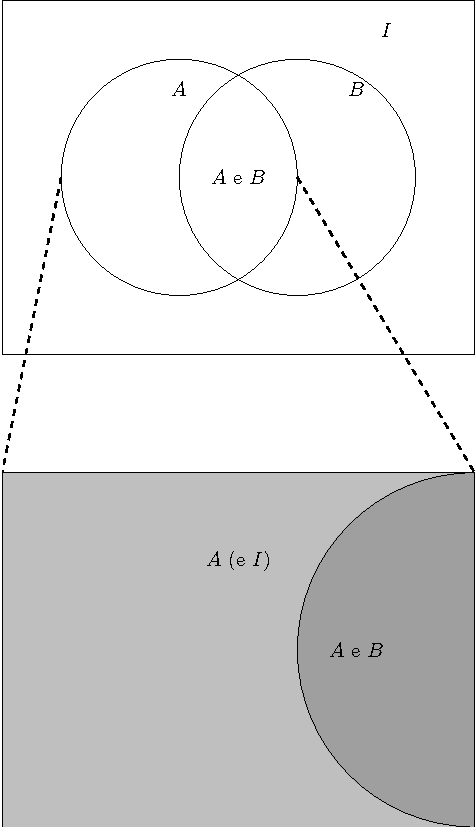
\includegraphics[keepaspectratio]{eventi_files/figure-pdf/unnamed-chunk-10-1.pdf}}

}

\caption{Rappresentazione della formula di Kolmogorov.}

\end{figure}%

\end{remark}

Dalla regola del prodotto, si ottiene la seguente variante della formula
di decomposizione, che possiamo chiamare per distiguerla come formula di
``disintegrazione'' (in inglese nota anche come \emph{law of total
probability}).

Sia \((A_i)_{i=1}^n\) un sistema di alternative rispetto ad una
informazione \(I\). Allora, data una affermazione \(B\) (qualsiasi), si
può decomporre \[ P(B|I) =  \sum_{i=1}^n P(B | A_i, I) P(A_i | I). \]

La dimostrazione a partire dalla formula di decomposizione è immediata:
basta osservare che, per ciascun \(i \in \cur{1, \ldots, n}\), vale per
la formula del prodotto \[ P(B | A_i, I) P(A_i | I)  = P(B, A_i | I). \]

Concludiamo questa sezione notando che per induzione matematica (ossia
ripetendo l'applicazione della formula del prodotto), si può ottenere la
seguente estensione al caso di \(n\) affermazioni qualsiasi \(B_1\),
\(B_2\), \ldots{} \(B_n\):
\[ P( \text{tutte le $B_i$ sono vere}) = P(B_1) P(B_2|B_1) P(B_3| B_1, B_2) \ldots P(B_n |B_1,B_2, \ldots, B_{n-1}).\]

\subsection{Esercizi}\label{esercizi-3}

Dedurre la proprietà di monotonia della probabilità dalla regola del
prodotto.

Scrivere esplicitamente la regola del prodotto generalizzata nei casi
\(n=3, 4, 5\).

\section{Diagrammi ad albero}\label{sec-alberi}

La formula di decomposizione combinata con la regola del prodotto e
delle sue conseguenze viste nella sezione precedente forniscono (quasi)
tutti gli strumenti utili per analizzare problemi di probabilità,
riducendoli a problemi più semplici: tutta l'arte sta nell'individuare
opportuni sistemi di alternative per cui il robot sia in grado di
calcolare agevolmente le varie probabilità condizionate.

È particolarmente utile rappresentare allora l'introduzione di sistemi
di sistemi di alternative tramite \textbf{diagrammi ad albero}, ossia di
grafi (insiemi di nodi collegati da archi) in cui ogni nodo è
etichettato da una affermazione (\(A\), \(B\), \(I\) ecc.) e gli archi
sono orientati e pesati con opportune probabilità, costruiti con il
seguente algoritmo.

Si introduce un nodo ``radice'' la cui etichetta è l'informazione
iniziale che si evince dal testo del problema (tipicamente si riserva la
lettera greca \(\Omega\) (omega) per tale informazione). Succesivamente
si itera un numero finito di volte la seguente procedura:

\begin{enumerate}
\def\labelenumi{\arabic{enumi}.}
\tightlist
\item
  si considera un nodo del grafo che sia una ``foglia'', ossia senza
  archi uscenti, etichettato da una affermazione \(B\),
\item
  si sceglie un sistema di alternative \((A_i)_{i=1}^n\), e si
  introducono tanti nodi quante le alternative, etichettate appunto da
  esse,
\item
  si introducono archi uscenti dalla foglia (\(B\)) verso il nodo
  corrispondente a ciascuna alternativa (\(A_i\)),
\item
  si pesa ciascun arco introdotto sopra con la probabilità
  \[P(A_i| B, I),\] dove \(I\) consiste della congiunzione di tutte le
  affermazioni nell'unico cammino (orientato) che collega l'informazione
  iniziale \(\Omega\) a \(B\).
\end{enumerate}

Si può mostrare che in questo modo si produce un grafo connesso e senza
cicli (detto quindi un albero). Un albero costruito opportunamente può
notevolmente semplificare le applicazioni delle regole di calcolo della
probabilità.

Consideriamo un esempio più concreto, introducendo il cosiddetto
\textbf{modello delle estrazioni da un'urna}. Supponiamo che vi sia una
scatola (urna) contenente un certo numero di palline, tra di loro
indistinguibili, eccetto che per il colore (che può essere \emph{rosso}
oppure \emph{blu}). Il robot è informato che l'urna contiene un numero
\(N\) palline di cui \(R\) sono rosse e \(B\) blu, con \(N\), \(R\),
\(B\) numeri noti (per fissare le idee, potrebbe essere \(R=3\), \(B=2\)
e quindi \(N=5\), ma teniamoli qui come parametri, per ottenere delle
formule generali). Una persona effettua un certo numero di
\textbf{estrazioni} di palline, una dopo l'altra, \textbf{senza
rimpiazzo}, ossia una volta tolte le palline e osservate, \emph{non}
vengono rimesse dentro l'urna (vedremo in seguito cosa cambia nel caso
con rimpiazzo, ossia se le palline vengono rimesse dentro l'urna).

Indichiamo allora con \(\Omega\) l'informazione iniziale descritta
sopra, e supponendo che la persona effettui \(n \le N\) estrazioni
(anche qui \(n\) è un parametro noto, ad esempio \(n=2\)), e per
ciascuna estrazione \(i =1, \ldots, n\) si introducono le due
alternative semplici
\[ R^i = \text{l'$i$-esima pallina estratta è rossa},\]
\[ B^i = \text{l'$i$-esima pallina estratta è blu}.\] Una domanda
naturale, cui il robot deve rispondere, è di calcolare
\[P(R^i | \Omega),\] ossia la probabilità di estrarre una pallina rossa
all'\(i\)-esima estrazione, senza che sia informato dell'esito di una
qualsiasi estrazione.

Il caso \(i=1\) è il più semplice da argomentare: la probabilità che si
estragga una pallina rossa dall'urna è \[ P( R^1 | I) = \frac{R}{N}.\]
Questo segue dal fatto che l'indistinguibilità delle palline (eccetto
per il colore) fa sì che la probabilità di estrarre una pallina
qualsiasi è uniforme (e vale \(1/N\)), mentre l'affermazione \(R^1\) si
scrive come disgiunzione (unione) tra \(R\) affermazioni (corrispondenti
alle \(R\) palline rosse): la regola della somma allora implica la
probabilità sopra. Notiamo che questo argomento mette in forma più
precisa l'intuizione che la probabilità sia il rapporto tra numero di
\emph{casi favorevoli} (\(R\)) e numero di \emph{casi totali} (\(N\)),
vero solamente se la densità discreta attribuita alle alternative (i
``casi'') sia uniforme.

Cosa accade alla seconda estrazione? Viene in aiuto la rappresentazione
ad albero descritta sopra. Iniziamo dalla radice \(\Omega\), cui
aggiungiamo il primo sistema di alternative \(R^1\), \(B^1\). Osserviamo
che le probabilità indicate sopra ciascun arco uscente (verso destra)
sommano ad \(1\), proprio perché è un sistema di alternative.

\begin{figure}[H]

{\centering \pandocbounded{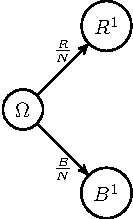
\includegraphics[keepaspectratio]{eventi_files/figure-pdf/unnamed-chunk-11-1.pdf}}

}

\caption{Diagramma ad albero per la prima estrazione.}

\end{figure}%

Concentriamoci ora sul calcolo di \(P(R^2 | \Omega)\), e decomponiamo
ciascuna foglia (i nodi più a destra) rispetto al sistema di alternative
\(R^2\), \(B^2\). Come determinare i pesi dati dalle probabilità
\(P(R^2 | R^1)\), \(P(R^2 | B^1)\) ecc.? Possiamo argomentare così: se
ad esempio si aggiunge l'informazione \(R^1\), significa che prima della
seconda estrazione il robot sa che l'urna contiene \(R-1\) palline rosse
e \(B\) blu. Dovendo usare solo questa informazione, segue usando una
sottostante probabilità uniforme che
\[ P(R^2 | R^1) = \frac{R-1}{N-1},\] e similmente per gli altri casi.

\begin{figure}[H]

{\centering \pandocbounded{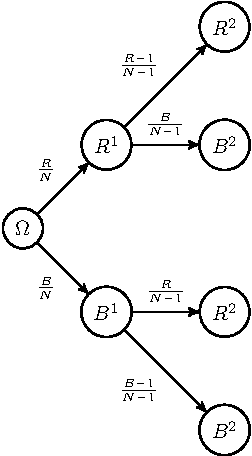
\includegraphics[keepaspectratio]{eventi_files/figure-pdf/unnamed-chunk-12-1.pdf}}

}

\caption{Diagramma ad albero per la prima e seconda estrazione.}

\end{figure}%

Possiamo calcolare quindi la probabilità \(P(R^2|\Omega)\). Usando la
formula di disintegrazione, troviamo (omettiamo \(\Omega\) per
semplicità)
\[ \begin{split} P(R^2  ) & = P(R^2 | R^1) P(R^1) + P(R^2 | B^1) P(B^1) \\
& = \frac{R-1}{N-1} \cdot \frac R N + \frac{R}{N-1}\cdot \frac{B}{N-1} = \frac R N.\end{split}\]
Possiamo allora ritrovare lo stesso risultato direttamente sfruttando
l'albero, nel seguente modo:

\begin{enumerate}
\def\labelenumi{\arabic{enumi}.}
\tightlist
\item
  per ciascun cammino (``ramo'') che collega il nodo \(\Omega\) ad una
  foglia corrispondente all'evento \(R^2\), si determina la probabilità
  ottenuta moltiplicando i pesi corrispondenti agli archi percorsi,
\item
  si sommano tutte le probabilità così ottenute.
\end{enumerate}

Nell'esempio, abbiamo due soli rami e si trova esattamente la stessa
formula per la probabilità di \(R^2\).

Ma possiamo anche fare di più, una volta decomposto un problema in un
albero abbastanza dettagliato, possiamo calcolare la probabilità di una
qualsiasi affermazione \(C\) (in questo caso, riguardante le prime due
estrazioni). Basta infatti aggiungere un nodo etichettato con l'evento
\(C\) a ciascuna foglia dell'albero già costruito (con un arco pesato
con la probabilità condizionata, come nell'algoritmo di costruzione
dell'albero) e calcolare la probabilità con lo stesso metodo, ossia
sommando le probabilità corrispondenti a ciascun ramo, partendo dalla
radice fino a \(C\). Ad esempio, sia
\[ C = \text{nelle prime due estrazioni si estraggono due palline dello stesso colore}.\]
Aggiungiamo \(C\) all'albero nel seguente modo.

\begin{figure}[H]

{\centering \pandocbounded{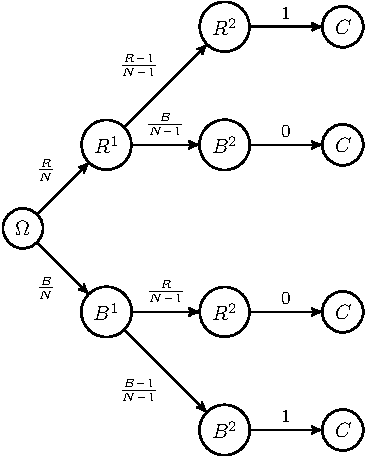
\includegraphics[keepaspectratio]{eventi_files/figure-pdf/unnamed-chunk-13-1.pdf}}

}

\caption{Un diagramma ad albero per l'evento \(C\).}

\end{figure}%

Calcolando la probabilità di ciascun ramo (notiamo che due hanno un peso
nullo, quindi possiamo trascurarli) e sommando su tutti i rami, troviamo
quindi che
\[ P(C) = \frac{R}N \cdot \frac{R-1}{N-1} + \frac B N \cdot \frac{B-1}{N-1}.\]

La validità di questa tecnica si estende ad alberi arbitrariamente
complessi, purché si faccia attenzione a due aspetti fondamentali
quando, a partire da una foglia, si introduce un sistema di alternative:

\begin{enumerate}
\def\labelenumi{\arabic{enumi}.}
\tightlist
\item
  \emph{tutte} le alternative vanno inserite (eccetto quelle
  trascurabili, che possono essere tralasciate)
\item
  i pesi degli archi inseriti sono probabilità condizionate rispetto a
  \emph{tutta} l'informazione complessiva dalla foglia fino alla radice.
\end{enumerate}

Un controllo da fare per evitare l'errore comune di tralasciare qualche
alternativa è di verificare che la somma delle probabilità sugli archi
uscenti da ciascun nodo sia sempre \(1\).

Osserviamo infine che \emph{non} è necessario, come negli esempi visti,
che l'albero sia ottenuto usando lo stesso sistema di alternative ad
ogni passo della costruzione: a partire da una foglia siamo liberi di
scegliere se proseguire con la costruzione e, nel caso, un sistema di
alternative che riteniamo utile. Bisogna infatti bilanciare tra la
necessità di creare un diagramma sufficientemente dettagliato e d'altra
parte non introdurre troppe ramificazioni, che rendono i calcoli
complicati con il rischio di perdere qualche termine nel corso della
risoluzione.

Ad esempio, se è richiesta la probabilità di
\[ D = \text{si estrae almeno una pallina blu nelle prime tre estrazioni},\]
possiamo creare un albero in cui interrompiamo la costruzione nelle
foglie in cui una pallina blu è estratta:

\begin{figure}[H]

{\centering \pandocbounded{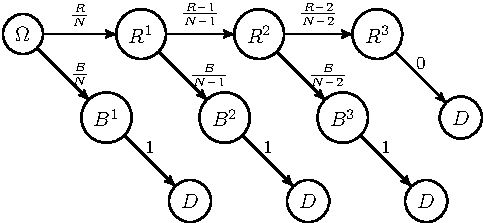
\includegraphics[keepaspectratio]{eventi_files/figure-pdf/unnamed-chunk-14-1.pdf}}

}

\caption{Un diagramma per il calcolo della probabilità di estrarre
almeno una pallina blu in tre estrazioni.}

\end{figure}%

Otteniamo quindi
\[ P(D ) = \frac B N + \frac{R} N \cdot \frac {B}{N-1} + \frac R N \cdot \frac {R-1}{N-1}\cdot \frac{B}{N-2}.\]
Concludiamo osservando che il modello delle estrazioni senza rimpiazzo è
abbastanza semplice per poter ottenere molte formule esplicite per la
probabilità di affermazioni interessanti. Ad esempio, tramite un uso
ripetuto della regola del prodotto, si ottiene che la probabilità
(rispetto all'informazione inizale \(\Omega\)) di estrarre una
\textbf{precisa sequenza ordinata} di \(n \le N\) palline colorate, di
cui \(r \le R\) sono rosse e le rimanenti \(b \le B\) sono blu è data
dalla formula
\[ \frac{R(R-1)\cdot \ldots \cdot (R-r+1) \cdot B(B-1) \cdot \ldots \cdot  (B-b+1)}{N(N-1)\cdot \ldots (N-n+1)}.\]
Ad esempio,
\[ P( R^1, B^2, R^3, B^4, R^5, B^6 ) = \frac{ R(R-1)(R-2)B(B-1)(B-2)}{N(N-1)(N-2)(N-3)(N-4)(N-5)}.\]
In particolare, la probabilità \emph{non} dipende dall'ordine in cui le
palline rosse e blu vengono estratte nella precisa sequenza. Perciò,
grazie alla regola della somma, possiamo anche ottenere la probabilità
di estrarre una \textbf{qualsiasi sequenza} di \(n \le N\) palline, di
cui \(r \le R\) rosse e le rimanenti \(n-r=b \le B\) sono blu: si tratta
di moltiplicare la probabilità di ottenere una di queste (ad esempio
quella in cui si estraggono prima \(r\) rosse e poi \(b\) blu) per il
numero totale di tali sequenze. Tale numero, è detto
\textbf{coefficiente binomiale} e si scrive
\[ {n \choose r} = \frac{n(n-1) \cdot \ldots \cdot (n-r+1)}{r (r-1) \cdot\ldots  \cdot 1} = \frac{ n!}{r! (n-r)!},\]
dove nell'ultima espressione abbiamo usato la funzione fattoriale
\[ k! = k(k-1)\cdot \ldots \cdot 1.\]

Con semplici passaggi algebrici, si ottiene una formula piuttosto
elegante, che usa solamente opportuni coefficienti binomiali:
\[ P( \text{si estrae una qualsiasi sequenza con $r$ rosse e $b$ blu} | \Omega) = \frac{{R \choose r} {B \choose b}}{ {N \choose n}}.\]
Osserviamo che, fissata la lunghezza \(n\), al variare di
\(r \in \cur{0, \ldots, n}\), le affermazioni \(A_r =\) ``si estrae una
qualsiasi sequenza con \(r\) rosse e \(b\) blu'', costituiscono un
sistema di alternative. La formula è quindi la densità discreta di
alternative (rispetto all'informazione iniziale \(\Omega\)) ed è detta
per ragioni storiche \textbf{densità ipergeometrica}.

\subsection{Esercizi}\label{esercizi-4}

Tracciare un grafico a barre della densità ipergeometrica per i
parametri \(N=10\), \(R= 5\) ed \(n=6\), e determinarne la moda (si
consiglia di usare il comando \texttt{dhyper()}).

Vi sono due urne dall'esterno indistinguibili, ciascuna contenente \(3\)
palline: la prima contiene \(1\) pallina rossa e due blu, la seconda
\(2\) rosse e una blu. Si sceglie a caso un'urna tra le due e si estrae
una pallina. Quale probabilità il robot attribuisce all'evento \(R^1\)?
e all'evento ``\(R^1 \text{ e } R^2\)''?

\section{Formula di Bayes}\label{sec-bayes}

Una conseguenza elementare della regola della somma è che, essendo
``\(A\) e \(B\)'' logicamente equivalente a ``\(B\) e \(A\)'', si può
anche scrivere (omettendo \(I\) per semplicità di notazione)
\begin{equation}\protect\phantomsection\label{eq-rapportosym}{
P( B ) P(A|B) = P(B \text{ e } A ) = P(A \text{ e } B) = P(A) P(B|A). 
}\end{equation}

Da questa semplice osservazione, dividendo per \(P(B)\) (supponendo che
non sia zero) segue una delle formule più importanti, ma anche discusse
e misinterpretate, del calcolo delle probabilità: la formula di Bayes.

Date affermazioni \(A\), \(B\) e l'informazione nota \(I\), vale
\[ P( A | B, I ) = P(A | I ) \frac{ P(B | A,I)}{P(B|I)}\] (purché
\(P(B|I)>0\)).

L'intepretazione della formula, apparentemente banale, è centrale.
Supponiamo che sia richiesto al robot di calcolare come l'acquisizione
di nuova informazione \(B\), oltre a quella già nota \(I\), cambi il
grado di fiducia nella validità di una affermazione \(A\). Allora la
formula di Bayes prescrive di aggiornare la probabilità (a volte detta
\textbf{a priori}) \(P(A|I)\) moltiplicandola per il rapporto
\begin{equation}\protect\phantomsection\label{eq-rapportobayes}{
\frac{ P(B | A,I)}{P(B|I)}.  
}\end{equation} La probabilità \(P(A|B,I)\) è detta anche \textbf{a
posteriori} (ossia dopo aver incluso l'informazione \(B\)). Teniamo
presente però che la distinzione \emph{a priori} e \emph{a posteriori} è
solamente nel momento in cui si applica la formula di Bayes, perché la
probabilità a posteriori \(P(A|B,I)\) a sua volta può diventare a priori
se si vuole includere ulteriore informazione \(C\), e calcolare
\(P(A|C,B,I)\), e così via.

Il numeratore nel rapporto Equazione~\ref{eq-rapportobayes}, ossia il
termine \[ P(B|A,I)\] è detto \textbf{verosimiglianza} (in inglese
\emph{likelihood}) di \(A\) rispetto a \(B\) (condizionata ad \(I\)) e
si indica tradizionalmente con la lettera \(L\) (eventualmente corsivo
\(\mathcal{L}\)). Noi useremo la notazione \[L(A; B) = P(B|A),\]
tralasciando di specificare \(I\), oppure \(L(A,I;B)\) se vogliamo
indicarla. La verosimiglianza di \(A\) rispetto a \(B\) è quindi
definita come la probabilità di \(B\) sapendo \(A\), e non è un concetto
nuovo, solamente una notazione in cui privilegiamo il ruolo \(A\)
rispetto a \(B\).

Il rapporto Equazione~\ref{eq-rapportobayes} che nella formula di Bayes
moltiplica la probabilità a priori (ossia rispetto ad \(I\)) può essere
maggiore, minore o uguale ad \(1\), e indica quanto il grado di fiducia
in \(B\) cambia se aggiungiamo invece l'informazione \(A\) --
qualitativamente, un rapporto maggiore di \(1\) indica che \(A\) è un
``indizio'' a favore della validità di \(B\). La formula di Bayes allora
permette di scambiare i ruoli di \(A\) e \(B\), un po' come se
invertissimo l'ipotesi con la tesi in un teorema: mentre questa
operazione nella logica deduttiva non è ammessa\footnote{un teorema non
  rimane vero in generale se scambiamo ipotesi con tesi}, nel calcolo
delle probabilità è possibile e anche molto utile, proprio perché a
volte è più facile ragionare scambiando i ruoli!

\begin{remark}
Consideriamo l'affermazione ``se piove, allora porto l'ombrello''.
Scambiando ipotesi con tesi si ottiene ``se porto l'ombrello, allora
piove''. Siccome ci tengo molto a non bagnarmi, la prima versione è
vera, ma la seconda non lo è necessariamente -- capita a volte che porti
l'ombrello per eccessiva precauzione. Però una persona, incontrandomi in
un corridoio mentre porto l'ombrello, è portata a pensare che fuori stia
piovendo. Per molti versi la formula di Bayes è più vicina al
ragionamento di \emph{buon senso} che applichiamo quotidianamente,
invece della mera deduzione logica.
\end{remark}

\subsection{Esercizi}\label{esercizi-5}

Si effettuano \(2\) estrazioni senza rimpiazzo da un'urna con \(N\)
palline, di cui \(R\) rosse e le rimanenti \(B\) blu (supporre che siano
parametri noti). Sapendo che la seconda estrazione è rossa, calcolare la
probabilità che la prima estrazione sia pure rossa.

Mostrare la seguente estensione della formula di Bayes: date
affermazioni \(A\), \(B\), \(I\) e \(J\), vale
\[ P( A, J | B, I) = P(A | I) \cdot \frac{ P(B, J | A, I)}{P(B|I)}.\]
Questa formula permette di scambiare ``parzialmente'' i ruoli
dell'informazione nota e dell'affermazione di cui si richiede la
probabilità.

\section{Statistica bayesiana}\label{sec-bayes-stat}

Dato un sistema di alternative \((A_i)_{i=1}^n\) (rispetto ad una
informazione \(I\) che qui sottointendiamo per alleggerire la notazione)
e una qualsiasi affermazione \(B\), possiamo applicare la formula di
Bayes a ciascuna alternativa e ottenere
\begin{equation}\protect\phantomsection\label{eq-bayes-alternative}{ 
P(A_i | B ) = P(A_i)  P(B | A_i ) \cdot \frac{1}{P(B)}, 
}\end{equation} dove abbiamo messo in evidenza il denominatore \(P(B)\)
per due ragioni. Da un lato, possiamo calcolarlo sempre tramite lo
stesso sistema di alternative e la formula di disintegrazione, ossia
\[ P(B) = \sum_{i=1}^n P(A_i)  P(B | A_i ).\] Questa identità permette
di ottenere una formula esplicita per la densità discreta del sistema di
alternative, rispetto alla nuova informazione che include \(B\) (oltre
ad \(I\)).

D'altra parte, non è neppure necessario usare la formula di
disintegrazione per calcolare \(P(B)\) perché, osservando la formula
Equazione~\ref{eq-bayes-alternative}, il membro a sinistra definisce la
densità discreta associata al sistema di alternative \((A_i)_{i=1}^n\)
rispetto alla nuova informazione che include \(B\) oltre ad \(I\).
Perciò, possiamo sempre indicarlo a meno di una costante moltiplicativa
comune (in questo caso appunto \(P(B)\)):
\begin{equation}\protect\phantomsection\label{eq-bayes-prop}{ 
P(A_i | B ) \propto P(A_i)  P(B | A_i )  = P(A_i)L(A_i;B), 
}\end{equation} avendo usato la verosimiglianza nella seconda
espressione. La probabilità di ciascuna alternativa rispetto alla nuova
informazione \(B\) è dunque ottenuta moltiplicando la probabilità
iniziale per la verosimiglianza associata. Ovviamente imponendo che la
somma delle probabilità sia \(1\) si trova la stessa formula per
\(P(B)\), o equivalentemente usando la notazione per la verosimiglianza
\[ P(B) = \sum_{i=1}^n P(A_i) L(A_i; B).\]

È quindi utile riconoscere che il denominatore \(P(B)\) ha un ruolo
secondario, e volendo si può tenere a mente solo la versione
(Equazione~\ref{eq-bayes-prop}) della formula. Un altra ragione per non
concentrarsi troppo sul denominatore comune \(P(B)\) è perché spesso non
si richiede di determinare quanto sia probabile ciascuna alternativa
\(A_i\), rispetto alla nuova informazione \(B\), ma semplicemente ci si
limita a determinare quale sia l'alternativa più probabile della nuova
densità discreta \((P(A_i|B))_{i=1}^n\). Abbiamo introdotto in
precedenza il termine statistico \emph{moda}, ma nel contesto della
formula di Bayes è detta stima del \textbf{massimo a posteriori} (in
inglese \emph{maximum a posteriori probability estimate}, MAP). Per
calcolare tale \(i_{\map} \in \cur{1, \ldots n}\), possiamo quindi
tralasciare costanti moltiplicative (positive) e allora vale
\[ i_{\map} \in \operatorname{arg} \max\cur{ P(A_i)  P(B | A_i )\, : \, i \in \cur{1, \ldots, n} }, \]
oppure, usando la notazione della verosimiglianza,
\[ i_{\map} \in \operatorname{arg} \max\cur{ P(A_i)  L( A_i ;B )\, : \, i \in \cur{1, \ldots, n} }, \]
dove ricordiamo che il simbolo di appartenenza (\(\in\)) è perché
potrebbero esserci più indici che raggiungono il massimo.

\begin{remark}[massima verosimiglianza]
Nel caso speciale in cui la densità discreta a priori sia uniforme,
ossia \(P(A_i) \propto 1\), si può ridurre ulteriormente il problema di
massimizzare \(P(A_i) P(B | A_i )\) alla semplice massimizzazione della
verosimiglianza \(P(B| A_i)=L(A_i;B)\). Tale approccio, molto utilizzato
in pratica perché spesso non si è in grado di precisare densità a priori
non uniformi, è detto stima di \textbf{massima verosimiglianza} (in
inglese \emph{maximum likelihood estimation}, MLE): dato un sistema di
alternative \((A_i)_{i=1}^n\) e una affermazione \(B\), avendo osservato
\(B\) si determina \(i_{\mle}\) tale che
\[ L(A_{i_{\mle}}; B)  = \max_{i=1, \ldots, n}L(A_i; B).\] Questo metodo
si può presentare anche senza la formula di Bayes, ma alla luce di
questa ne abbiamo una giustificazione in termini del calcolo delle
probabilità, e anche una sua estensione al caso in cui le probabilità a
priori non siano uniformi.
\end{remark}

\begin{remark}[passaggio al logaritmo]
Ricordando che è possibile anche passare al logaritmo per determinare la
moda, si può quindi determinare
\[  i_{\map} \in \operatorname{arg} \max\cur{ \log( P(A_i)) + \log( L( A_i ;B ))\, : \, i \in \cur{1, \ldots, n} }, \]
che nel caso di densità a priori uniforme si ridure a massimizzare la
\(\log\)-verosimiglianza (\(\log\)-likelihood in inglese)
\(\log( L(A_i; B))\) sulle possibili alternative \((A_i)_{i\in I}\).
\end{remark}

Vediamo in pratica un esempio dal modello delle estrazioni senza
rimpiazzo dall'urna. Questa volta, il robot \emph{non} è inizialmente
informato sul numero di palline rosse contenute, ma solamente sul numero
totale \(N=3\). Dopo un'estrazione, si aggiorna il robot con
l'informazione \(R^1\), ossia che una pallina rossa è stata estratta.
Cosa può dedurre circa il contenuto dell'urna? Usando il calcolo delle
probabilità sviluppato finora e in particolare la formula di Bayes,
diamo una risposta (questo modo di procedere è detto anche
\textbf{statistica Bayesiana}).

Introduciamo un sistema di alternative relativo al contenuto dell'urna:
\[ A_i = \text{l'urna contiene $R=i$ palline rosse}, \] per
\(i \in \cur{0,1, 2, 3}\). Prima di poter applicare la formula di Bayes,
il robot deve stabilire la densità discreta associata al sistema
rispetto all'informazione inizale (la probabilità \emph{a priori}). È
chiaro che potrebbero esserci molteplici scelte, ma non avendo ragioni
per favorire una alternativa rispetto all'altra, questa è proprio una
situazione in cui usare la densità discreta uniforme. Pertanto,
indicando con \(\Omega\) l'informazione iniziale, per ciascun
\(i\in \cur{0,1,2,3}\), il robot pone \[ P(A_i | \Omega) = \frac 1 4.\]
Successivamente, il robot calcola la probabilità condizionata (il
problema conoscendo il numero di palline rosse e blu è già stato
affrontato nella sezione precedente) \[ P( R^1 | A_i) = \frac{i}{3},\] e
conclude, usando la formula di Bayes
\[ P(A_i | R^1 ) = \frac{1}{4} \cdot \frac{i}{3} \cdot \frac{1}{P(R^1|\Omega)} \propto i.\]
Anche senza calcolare \(P(R^1|\Omega)\), si vede subito che
l'alternativa più probabile è \(i_{\max} = 3\), ossia l'urna contiene
solo palline rosse -- questa è anche la risposta mediante massima
verosimglianza. Osserviamo anche un fatto banale, ma che ci rassicura:
vale \(P(A_0 | R^1) = 0\), perché il robot è ora certo che vi sia almeno
una pallina rossa.

Possiamo confrontare la densità discreta con un grafico a barre:

\begin{Shaded}
\begin{Highlighting}[]
\CommentTok{\# Calcoliamo vettori delle densità a priori e dopo aver osservato R\^{}1}

\NormalTok{(dens\_apriori }\OtherTok{\textless{}{-}}\FunctionTok{rep}\NormalTok{(}\DecValTok{1}\SpecialCharTok{/}\DecValTok{4}\NormalTok{, }\DecValTok{4}\NormalTok{))}
\end{Highlighting}
\end{Shaded}

\begin{verbatim}
[1] 0.25 0.25 0.25 0.25
\end{verbatim}

\begin{Shaded}
\begin{Highlighting}[]
\NormalTok{dens\_R1 }\OtherTok{\textless{}{-}} \DecValTok{0}\SpecialCharTok{:}\DecValTok{3}
\NormalTok{(dens\_R1 }\OtherTok{\textless{}{-}}\NormalTok{ dens\_R1}\SpecialCharTok{/}\FunctionTok{sum}\NormalTok{(dens\_R1))}
\end{Highlighting}
\end{Shaded}

\begin{verbatim}
[1] 0.0000000 0.1666667 0.3333333 0.5000000
\end{verbatim}

\begin{Shaded}
\begin{Highlighting}[]
\CommentTok{\# Per il grafico a barre vanno inseriti in una matrice}

\NormalTok{dens\_matrice }\OtherTok{\textless{}{-}} \FunctionTok{matrix}\NormalTok{( }\FunctionTok{c}\NormalTok{(dens\_apriori, dens\_R1), }\AttributeTok{nrow=}\DecValTok{2}\NormalTok{, }\AttributeTok{byrow=}\ConstantTok{TRUE}\NormalTok{)}

\CommentTok{\# Alcuni parametri per il grafico e il comando barplot()}

\NormalTok{alternative }\OtherTok{\textless{}{-}} \FunctionTok{as.character}\NormalTok{(}\DecValTok{0}\SpecialCharTok{:}\DecValTok{3}\NormalTok{)}
\NormalTok{colori }\OtherTok{\textless{}{-}}\NormalTok{ miei\_colori[}\DecValTok{1}\SpecialCharTok{:}\DecValTok{2}\NormalTok{]}

\FunctionTok{barplot}\NormalTok{(dens\_matrice, }\AttributeTok{beside =} \ConstantTok{TRUE}\NormalTok{, }\AttributeTok{col=}\NormalTok{colori, }\AttributeTok{names.arg =}\NormalTok{ alternative, }\AttributeTok{ylab=}\StringTok{"probabilità"}\NormalTok{, }\AttributeTok{xlab=}\StringTok{"alternativa"}\NormalTok{)}

\CommentTok{\# Aggiungiamo infine una legenda}

\FunctionTok{legend}\NormalTok{(}\StringTok{\textquotesingle{}top\textquotesingle{}}\NormalTok{,}\AttributeTok{fill=}\NormalTok{colori,}\AttributeTok{legend=}\FunctionTok{c}\NormalTok{(}\StringTok{\textquotesingle{}A priori\textquotesingle{}}\NormalTok{,}\StringTok{\textquotesingle{}Sapendo R\^{}1\textquotesingle{}}\NormalTok{), }\AttributeTok{cex =} \FloatTok{0.8}\NormalTok{)}
\end{Highlighting}
\end{Shaded}

\begin{figure}[H]

{\centering \pandocbounded{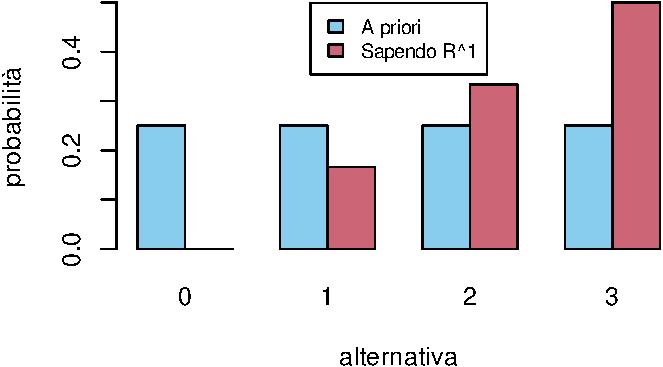
\includegraphics[keepaspectratio]{eventi_files/figure-pdf/unnamed-chunk-15-1.pdf}}

}

\caption{Densità discreta delle alternative a priori e dopo una
estrazione.}

\end{figure}%

\begin{remark}[decisioni e test statistici]
Dopo aver osservato \(R^1\) e determinato l'alternativa più probabile,
in questo caso \(A_3\), ossia l'urna contiene solo palline rosse, si può
affermare con abbastanza sicurezza che la realtà sia proprio questa?
L'approccio di massima verosimiglianza darebbe appunto questa
indicazione, ma è ovvio in questo caso che, essendo la probabilità
\(P(A_3|R^1) = 1/2\), l'incertezza è ancora grande.

Nella pratica, il calcolo delle probabilità serve spesso appunto a
valutare l'incertezza sugli effetti di intraprendere determinate
iniziative e indicare quindi quali \textbf{decisioni} mettere in
pratica. Almeno una volta nella vita avremo guardato le previsioni del
tempo e sulla base della probabilità che piova abbiamo stabilito se
organizzare un'uscita nel fine settimana. Una decisione in ogni caso
realistico è basata su molti altri aspetti, oltre al fatto che
l'alternativa sia la più probabile: esiste una intera
\href{https://it.wikipedia.org/wiki/Teoria_della_decisione}{teoria della
decisione} che si occupa di questo problema, specialmente dal punto di
vista economico/utilitario.

Un punto di vista analogo, ma tradizionalmente legato al metodo
scientifico di alcune discipline, è fornito dalla teoria dei
\textbf{test statistici}: le alternative \(A_i\) sono pensate come
``ipotesi'' e sulla base delle osservazioni si decide quali siano
confutate/falsificate e pertanto vadano scartate (il termite tecnico è
\textbf{rifiutate}). Le rimanenti ipotesi sono quindi ``accettate'', ma
sempre con il beneficio del dubbio, nello stesso senso in cui una teoria
scientifica rimane valida fintanto che non si trova un esperimento che
ci indichi che qualcosa non va e pertanto debba essere modificata.

Tecnicamente, nei test statistici le alternative vengono collezionate in
due sottoinsiemi disgiunti, detti rispettivamente l'ipotesi nulla (e
indicato con \(\mathcal{H}_0\)) e l'alternativa (indicato con
\(\mathcal{H}_1\)). L'attenzione principale è rivolta a rifiutare
l'ipotesi nulla, ossia scartare tutte le alternative
\(A_i \in \mathcal{H}_0\) (questa è in un certo senso la decisione da
prendere o meno sulla base della evidenza \(B\)). Se si osserva che
\(B\) vale, si decide di rifiutare l'ipotesi nulla se la probabilità che
\(B\) sia vero, condizionata a una qualsiasi \(A_i\) tra quelle
dell'ipotesi nulla \(\mathcal{H}_0\) è troppo bassa. Si stabilisce
quindi una soglia (detto tecnicamente \textbf{livello di
significatività} del test, spesso indicato con \(\alpha \in (0,1)\))
sotto la quale si ritiene troppo poco probabile che \(B\) possa essere
vero se vale una qualsiasi \(A_i\) dell'ipotesi nulla, e quindi
\(\mathcal{H}_0\) va scartato, a favore di \(\mathcal{H}_1\). La
quantità centrale della teoria dei test statistici è quindi il valore
\(p\) (in inglese \(p\)-value) introdotto da Fisher, definito (con la
nostra notazione), come
\[ p = \max_{A_i \in \mathcal{H}_0} P(B | A_i) = \max_{A_i \in \mathcal{H}_0} L(A_i; B).\]
Se \(p\) è minore del livello di significatività \(\alpha\), significa
che assumendo una qualsiasi \(A_i\) tra quelli dell'ipotesi nulla
\(\mathcal{H}_0\), la probabilità che \(B\) sia vero è comunque minore
di \(\alpha\), e quindi se si osserva \(B\) si decide di rifiutare
\(\mathcal{H}_0\). Più piccolo è il valore \(p\), minore è la
probabilità che \(B\) sia vero rispetto a l'ipotesi \(\mathcal{H}_0\), e
quindi saremo più sicuri nel rifiutarla.

Osserviamo però che con questo metodo non ci si domanda quanto \(B\)
fosse probabile se si assume una \(A_i\) tra quelle delle
\(\mathcal{H}_1\): si potrebbe criticare quindi che l'ipotesi venga
scartata semplicemente perché \(B\) è sempre poco probabile (ma comunque
la decisione interviene solo se lo si è osservato nella realtà). Una
ulteriore critica è che, per determinare il valore \(p\), bisognerebbe
considerare la probabilità \(P(A_i |B)\), e non la verosimiglianza
\(P(B|A_i) = L(A_i; B)\), perché non necessariamente tutte le ipotesi a
priori sono ugualmente probabili. Ovviamente vi sono ulteriori tecniche
per mitigare i possibili usi errati della teoria dei test statistici che
sorgono dalle osservazioni critiche sopra. Quello dei test rimane
sicuramente uno strumento importante, ma spesso poco compreso (e a volte
usato erroneamente).
\end{remark}

Torniamo all'esempio dell'urna, e chiediamoci cosa deduce il robot se
viene informato che alla seconda estrazione (senza rimpiazzo) la pallina
estratta è blu. Si tratta allora di condizionare anche rispetto a
\(B^2\). Notiamo che non serve tornare alla densità iniziale (uniforme),
ma basta usare come nuova densità \emph{a priori} la densità discreta
rispetto all'informazione \(R^1\), e si trova
\[ P(A_i | R^1,B^2 ) =  P(A_i|R^1) P(B^2 | R^1,A_i) \cdot \frac{1}{P(B^2|R^1)}.\]
Se vale \(A_i\), allora sapendo \(R^1\) ci sono due palline nell'urna,
di cui \(3-i\) blu (purché \(i \neq 0\)), quindi
\[P(B^2 |R^1, A_i) = \frac{3-i}{2}.\] Si ottiene allora che
\[ P(A_i|R^1, B^2) \propto i (3-i)\] e quindi la probabilità rilusta
uniforme, ma solamente sulle alternative \(A_1\), \(A_2\) (d'altra parte
\(A_0\) e \(A_3\) sono diventate trascurabili). Possiamo anche
confrontarle in un grafico a barre.

\begin{Shaded}
\begin{Highlighting}[]
\CommentTok{\# La "nuova" densità a priori è quella ottenuta prima, avendo osservato R\^{}1, perciò basta definire la densità avendo osservato anche B\^{}2}

\NormalTok{dens\_B2\_R1 }\OtherTok{\textless{}{-}}\NormalTok{ dens\_R1 }\SpecialCharTok{*} \DecValTok{3}\SpecialCharTok{:}\DecValTok{0}
\NormalTok{(dens\_B2\_R1 }\OtherTok{\textless{}{-}}\NormalTok{ dens\_B2\_R1}\SpecialCharTok{/}\FunctionTok{sum}\NormalTok{(dens\_B2\_R1))}
\end{Highlighting}
\end{Shaded}

\begin{verbatim}
[1] 0.0 0.5 0.5 0.0
\end{verbatim}

\begin{Shaded}
\begin{Highlighting}[]
\CommentTok{\# Per il grafico a barre le inseriamo tutte in una matrice}

\NormalTok{dens\_matrice }\OtherTok{\textless{}{-}} \FunctionTok{matrix}\NormalTok{( }\FunctionTok{c}\NormalTok{(dens\_apriori, dens\_R1, dens\_B2\_R1), }\AttributeTok{nrow=}\DecValTok{3}\NormalTok{, }\AttributeTok{byrow=}\ConstantTok{TRUE}\NormalTok{)}

\CommentTok{\# Alcuni parametri per il grafico e il comando barplot()}
 
\NormalTok{alternative }\OtherTok{\textless{}{-}} \FunctionTok{as.character}\NormalTok{(}\DecValTok{0}\SpecialCharTok{:}\DecValTok{3}\NormalTok{)}
\NormalTok{colori }\OtherTok{\textless{}{-}}\NormalTok{ miei\_colori[}\DecValTok{1}\SpecialCharTok{:}\DecValTok{3}\NormalTok{]}
\FunctionTok{barplot}\NormalTok{(dens\_matrice, }\AttributeTok{beside =} \ConstantTok{TRUE}\NormalTok{, }\AttributeTok{col=}\NormalTok{colori, }\AttributeTok{names.arg =}\NormalTok{ alternative, }\AttributeTok{ylab=}\StringTok{"probabilità"}\NormalTok{, }\AttributeTok{xlab=}\StringTok{"alternativa"}\NormalTok{)}

\CommentTok{\# Legenda}

\FunctionTok{legend}\NormalTok{(}\StringTok{\textquotesingle{}topleft\textquotesingle{}}\NormalTok{,}\AttributeTok{fill=}\NormalTok{colori,}\AttributeTok{legend=}\FunctionTok{c}\NormalTok{(}\StringTok{"A priori"}\NormalTok{,}\StringTok{"Sapendo R\^{}1"}\NormalTok{, }\StringTok{"Sapendo R\^{}1 e B\^{}2"}\NormalTok{), }\AttributeTok{cex =} \FloatTok{0.8}\NormalTok{)}
\end{Highlighting}
\end{Shaded}

\begin{figure}[H]

{\centering \pandocbounded{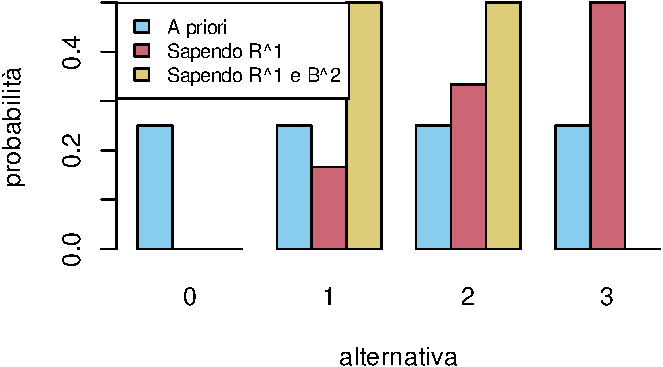
\includegraphics[keepaspectratio]{eventi_files/figure-pdf/unnamed-chunk-16-1.pdf}}

}

\caption{Densità discreta delle alternative fino a due estrazioni.}

\end{figure}%

È ovvio ma interessante comunque osservare come l'alternativa \(A_3\),
che dopo la prima estrazione era la più probabile, ora è trascurabile.
Inoltre il robot risulta completamente indeciso tra l'alternativa
\(A_1\) e l'alternativa \(A_2\). Aggiungere informazione in questo caso
ha aumentato la sua incertezza, e non rimane che effettuare l'ultima
estrazione per scoprire quale sia il colore della terza pallina!

\subsection{Esercizi}\label{esercizi-6}

Cosa accade nell'esempio sopra se il robot viene informato che le prime
due estrazioni sono invece \(R^1\), \(R^2\)? calcolare le probabilità e
confrontare visivamente le densità discrete ottenute mediante grafici a
barre.

Calcolare e plottare una variante dell'esempio sopra in cui \(N=6\),
inizialmente il robot non sa quante palline rosse vi siano e si informa
poi che nelle prime \(3\) estrazioni le palline estratte sono tutte
dello stesso colore (ma non si specifica quale).

\section{Indipendenza probabilistica}\label{sec-indipendenza}

Nella formula di Bayes vi è una certa simmetria, nel senso che il ruolo
di \(A\) e \(B\) può essere scambiato. Per metterla di più in evidenza,
notiamo che dividendo per il prodotto \(P(A)P(B)\) (assumendo che sia
positivo) l'equazione Equazione~\ref{eq-rapportosym}, otteniamo
\[  \frac{ P(A | B )}{P(A)} = \frac{P(A, B)}{P(A)P(B)} = \frac{ P(B | A )}{P(B)}. \]
(evitiamo per semplicità di scrivere \(I\)). In particolare, se
scambiamo \(A\) con \(B\) il rapporto che va a moltiplicare la
probabilità a priori nella formula di Bayes non cambia.
Qualitativamente, \(A\) è un indizio a favore della validità di \(B\)
(ossia il rapporto è maggiore di \(1\)) se e solo se \(B\) lo è per
\(A\), e analogamente se il rapporto è minore di \(1\). Se il rapporto è
proprio uguale ad \(1\) significa che il grado di fiducia della validità
di \(A\), pur sapendo l'informazione aggiuntiva \(B\), non cambia
(rispetto a non sapere \(B\)). Tale concetto prende il nome di
\textbf{indipendenza probabilistica}.

Due affermazioni \(A\), \(B\) si dicono indipendenti (condizionatamente
all'informazione nota \(I\)) se
\[ P(A| B,I) = P(A | I ) \quad \text{oppure} \quad  P(B| A,I) = P(B| I ),\]
oppure ancora \[ P(A, B|I) = P(A|I) P(B|I). \]

Il vantaggio dell'ultima identità è che non si divide per \(P(A|I)\) o
\(P(B|I)\), quindi non serve l'ipotesi che queste quantità siano non
nulle. È certamente anche più semplice da ricordare: si tratta di una
regola del prodotto ``semplificata''. Sebbene l'indipendenza sia una
condizione simmetrica, spesso si dice che \(A\) è indipendente da \(B\)
(o viceversa), ma il significato rimane lo stesso.

\begin{remark}
Un errore ricorrente è di confondere l'\emph{incompatibilità} tra due
affermazioni con l'\emph{indipendenza}. Si tratta di due concetti
estremamente diversi, anzi è facile vedere che se due affermazioni (non
trascurabili) sono incompatibili, allora il rapporto \(P(A|B)/P(A)\) è
nullo.
\end{remark}

Osserviamo che se \(A\), \(B\) sono indipendenti (rispetto ad \(I\), che
omettiamo), lo sono anche ``non \(A\)'' da \(B\), perché
\[ P( \text{non $A$} | B) = 1- P(A |  B) = 1 - P(A) = P( \text{non $A$}). \]
Sfruttando poi la simmetria dell'indipendenza segue che anche ``non
\(A\)'' è indipendente da ``non \(B\)'' e pure \(A\) da ``non \(B\)''.

Veniamo ora all'esempio fondamentale di indipendenza, ossia il modello
delle \textbf{estrazioni con rimpiazzo}. Informiamo il robot che vi è la
solita urna con \(N\) palline di cui \(R\) rosse e \(B\) blu, dove
\(N\), \(R\) e \(B\) sono parametri noti. Stavolta, dopo la prima
estrazione, la pallina viene osservata e rimessa all'interno dell'urna.
Dato che l'operazione è quindi cambiata in questo modo, come calcolare
la probabilità di un evento relativo ad una seconda estrazione, ad
esempio \(R^2\), sapendo \(R^1\)? Il robot potrebbe immaginare molte
situazioni in cui una prima estrazione rossa favorisce una seconda
estrazione rossa (ad esempio, viene rimessa in alto e chi estrae
preferisce estrarre dall'alto), ma anche altrettante in cui una seconda
estrazione rossa è sfavorita. Facendo appello alla razionalità del
robot, l'unica conclusione ragionevole è che, pur sapendo \(R^1\), nella
seconda estrazione si ha un'urna praticamente identica alla situazione
iniziale, con lo stesso numero di palline rosse e blu, e pertanto il
robot pone \[ P(R^2 | R^1 ) = \frac{R}{N}.\] Similmente, nel caso
condizionato a \(B^1\), \[ P(R^2 | B^1 ) = \frac{R}{N}.\] Completando
allora il diagramma ad albero con queste probabilità, si trova che
\[P(R^2|\Omega) = \frac{R}{N}\cdot \frac{R}{N} + \frac{B}{N}\cdot \frac{R}{N} = \frac{R}{N},\]
ossia \(P(R^2|R^1) = P(R^2)\) e quindi \(R^1\) ed \(R^2\) sono
indipendenti (rispetto all'informazione iniziale). Per quanto detto
sopra, segue che ogni evento relativo alla prima estrazione (\(R^1\),
\(B^1\)) è indipendente da ogni evento relativo alla seconda (\(R^2\),
\(B^2\)). Si dice pertanto che le due estrazioni sono indipendenti.

\begin{figure}[H]

{\centering \pandocbounded{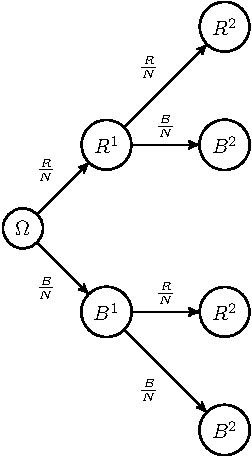
\includegraphics[keepaspectratio]{eventi_files/figure-pdf/unnamed-chunk-17-1.pdf}}

}

\caption{Diagramma ad albero per la prima e seconda estrazione, con
rimpiazzo.}

\end{figure}%

\begin{remark}
L'indipendenza probabilistica è quindi un'ipotesi che viene inserita,
essenzialmente perché non si riesce a proporre di meglio. Se il robot
fosse informato che chi estrae ha qualche preferenza, ad esempio tende a
ripescare l'ultima pallina estratta, dovrebbe abbandonare l'assunzione
di indipendenza. Per molti aspetti, sopratutto matematici e di
semplicità di calcolo, l'indipendenza è utile, ma forse tradizionalmente
viene posta troppa attenzione su questo concetto, dando l'impressione
che senza indipendenza non si possa fare molto. Ma in realtà è vero
l'opposto: l'apprendimento dalle osservazioni non potrebbe avere luogo
se vi fosse solo indipendenza, perché la formula di Bayes darebbe sempre
che le probabilità a priori non cambiano mai!
\end{remark}

Tornando alle estrazioni, come può ragionare il robot alla terza (avendo
rimesso nell'urna anche la seconda pallina estratta)? È naturale imporre
che, qualsiasi informazione \(J\) esso ottenga dalle prime due
estrazioni (ad esempio \(J = (R^1, R^2)\)), si avrà comunque che
\[ P(R^3 | J) = \frac{R}{N}.\] Possiamo allora costruire il diagramma ad
albero e ottenere con semplici calcoli che, anche in questo caso,
\[ P(R^3 ) = \frac R N,\] (avendo omesso di indicare l'informazione
iniziale \(\Omega\)). Pertanto, qualsiasi informazione sulle prime due
estrazioni non cambia il grado di fiducia sulla terza (lo stesso
discorso vale anche per \(B^3\)). Si può anche mostrare che, se il robot
acquisisce dell'informazione relativa a due qualsiasi estrazioni, la
probabilità di un evento relativo alla rimanente estrazione (delle prime
tre) non cambia. Ad esempio,
\[ P(R^1 | B^2, R^3) = \frac{R}{N} = P(R^1).\] Inoltre, usando la regola
del prodotto, otteniamo che
\[ P(R^1, B^2, R^3) = P(R^1) P(B^2 ) P(R^3 )\] Questo fatto, che deve
valere per ogni possibile scelta di eventi dai tre sistemi di
alternative relativi alle estrazioni, ci permette di intuire come
generalizzare il concetto di indipendenza da due a tre o più eventi. È
in realtà più semplice definire direttamente l'indipendenza tra sistemi
di alternative. Per ora diamo la seguente definizione, che riprenderemo
usando il linguaggio delle variabili aleatorie nel prossimo capitolo.

Dati \(k \ge 2\) sistemi di alternative \(\mathcal{S}_1\),
\(\mathcal{S}_2\), \ldots{} \(\mathcal{S}_k\), essi si dicono
indipendenti tra loro (rispetto all'informazione \(I\)) se
\[ P( A^1, A^2, \ldots, A^k | I) = \prod_{i=1}^n P(A^i|I), \] per ogni
scelta di \(A^1 \in \mathcal{S}_1\), \(A^2 \in \mathcal{S}_2\), \ldots{}
\(A^k \in \mathcal{S}_k\).

Tornando all'esempio delle estrazioni con rimpiazzo, il robot supporrà
allora che i sistemi di alternative \(\mathcal{S}_i = \cur{R^i, B^i}\)
relativi alle diverse estrazioni \(i=1, 2, \ldots\) siano tra loro
indipendenti. Possiamo allora chiedere, come nel caso delle estrazioni
senza rimpiazzo, quale sia la probabilità di osservare una
\textbf{specifica sequenza ordinata} lunga \(n\) di palline, di cui
\(r\) rosse e \(b\) blu. Notiamo che la sequenza può essere
arbitrariamente lunga, perché l'urna non si svuota mai. Usando la regola
del prodotto e l'indipendenza, si trova anche in questo caso che la
probabilità non dipende dall'ordine in cui i colori vengono osservati e,
rispetto al caso senza rimpiazzo, ha un'espressione anche più semplice:
\[ \bra{\frac{R}N}^r \bra{ \frac B N}^b = \bra{\frac{R}N}^r \bra{ 1- \frac R N}^{n-r},\]
avendo usato che \(B/N = 1-R/N\) e \(b = n-r\). Per semplificare
ulteriormente tare probabilità, si pone \(p = R/N \in [0,1]\) la
probabilità di estrarre una pallina rossa, e si trova
\[ p^r (1-p)^{n-r}.\] Come nel caso delle estrazioni senza rimpiazzo, se
chiediamo invece al robot la probabilità di estrarre una
\textbf{qualsiasi sequenza ordinata} lunga \(n\) e contenente \(r\)
palline rosse, basta moltiplicare la probabilità di una specifica
sequenza per il coefficiente binomiale (che conta il numero di tali
sequenze). Si trova quindi
\[ P( \text{si estrae con rimpiazzo una sequenza lunga $n$ con $r$ rosse} ) = {n \choose r} p^r (1-p)^{n-r}.\]
che definisce una nuova densità discreta sulle \(n+1\) alternative, al
variare di \(r \in \cur{0, \ldots, n}\). Essa è nota come
\textbf{densita binomiale} con parametri \(n\) (numero di estrazioni),
\(p \in [0,1]\) (frazione di palline rosse). Tale formula è
particolarmente ricorrente in tutte le situazioni in cui vi siano \(n\)
``esperimenti'' ripetuti e si chieda il numero di ``successi'' (nel
nostro caso, estrarre una pallina rossa), sotto l'ipotesi che tutti gli
esperimenti siano tra loro indipendenti e la probabilità di successo per
ciascun esperimento sia uguale a \(p\).

\begin{Shaded}
\begin{Highlighting}[]
\CommentTok{\# Usiamo la funzione dbinom() per ottenere direttamente la densità binomiale con i parametri cercati}

\NormalTok{n }\OtherTok{\textless{}{-}} \DecValTok{6}
\NormalTok{r }\OtherTok{\textless{}{-}} \DecValTok{0}\SpecialCharTok{:}\DecValTok{6}
\NormalTok{dens\_1\_3 }\OtherTok{\textless{}{-}} \FunctionTok{dbinom}\NormalTok{(r, n, }\DecValTok{1}\SpecialCharTok{/}\DecValTok{3}\NormalTok{)}
\NormalTok{dens\_1\_2 }\OtherTok{\textless{}{-}} \FunctionTok{dbinom}\NormalTok{(r, n, }\DecValTok{1}\SpecialCharTok{/}\DecValTok{2}\NormalTok{)}
\NormalTok{dens\_2\_3 }\OtherTok{\textless{}{-}} \FunctionTok{dbinom}\NormalTok{(r, n, }\DecValTok{2}\SpecialCharTok{/}\DecValTok{3}\NormalTok{)}

\NormalTok{dens\_matrice }\OtherTok{\textless{}{-}} \FunctionTok{matrix}\NormalTok{( }\FunctionTok{c}\NormalTok{(dens\_1\_3, dens\_1\_2, dens\_2\_3), }\AttributeTok{nrow =}\DecValTok{3}\NormalTok{, }\AttributeTok{byrow=}\ConstantTok{TRUE}\NormalTok{)}

\CommentTok{\# Grafico a barre e legenda}

\NormalTok{alternative }\OtherTok{\textless{}{-}} \FunctionTok{as.character}\NormalTok{(r)}
\NormalTok{colori }\OtherTok{\textless{}{-}}\NormalTok{ miei\_colori[}\DecValTok{1}\SpecialCharTok{:}\DecValTok{3}\NormalTok{]}
\FunctionTok{barplot}\NormalTok{( dens\_matrice, }\AttributeTok{beside=}\ConstantTok{TRUE}\NormalTok{, }\AttributeTok{col=}\NormalTok{colori, }\AttributeTok{names.arg=}\NormalTok{alternative, }\AttributeTok{ylab=}\StringTok{"probabilità"}\NormalTok{, }\AttributeTok{xlab=}\StringTok{"alternativa"}\NormalTok{)}

\FunctionTok{legend}\NormalTok{(}\StringTok{\textquotesingle{}topright\textquotesingle{}}\NormalTok{, }\AttributeTok{fill=}\NormalTok{colori, }\AttributeTok{legend=}\FunctionTok{c}\NormalTok{(}\StringTok{"p=1/3"}\NormalTok{, }\StringTok{"p=1/2"}\NormalTok{, }\StringTok{"p=2/3"}\NormalTok{), }\AttributeTok{cex=}\FloatTok{0.8}\NormalTok{)}
\end{Highlighting}
\end{Shaded}

\begin{figure}[H]

{\centering \pandocbounded{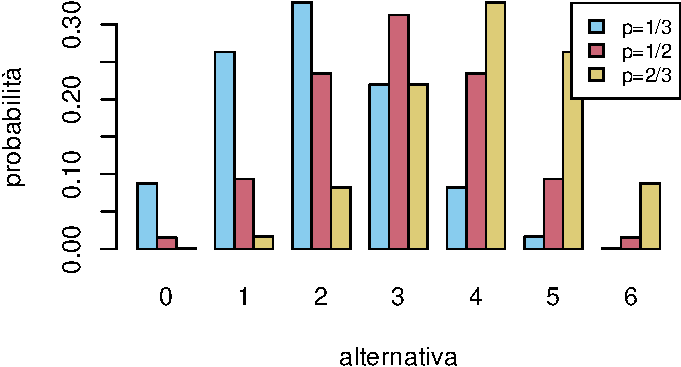
\includegraphics[keepaspectratio]{eventi_files/figure-pdf/unnamed-chunk-18-1.pdf}}

}

\caption{Grafici a barre della densità binomiale con parametri \(n=6\),
\(p=1/3\), \(p=1/2\), e \(p=2/3\).}

\end{figure}%

\subsection{Esercizi}\label{esercizi-7}

Ripetere l'esempio della Sezione~\ref{sec-bayes-stat} nel caso in cui le
estrazioni siano effettuate rimpiazzo.

Calcolare la probabilità di non estrarre mai una pallina rossa in
\(n=4\) estrazioni da un'urna con \(N=9\) palline di cui \(R=5\) rosse e
\(B=4\) blu, nei due casi di estrazioni (con e senza rimpiazzo). In
quale caso la probabilità è maggiore? Supponendo che il robot conosca il
contenuto dell'urna ma non sappia quale tra le due modalità di
estrazione viene svolta, calcolare e rappresentare con un grafico a
barre la probabilità che le estrazioni siano senza rimpiazzo, avendo
osservato solo palline blu nelle prime \(n\) estrazioni, per \(n=1\),
\(n=2\), \(n=3\) de \(n=4\).

\section{Gli assiomi di Kolmogorov}\label{sec-assiomi}

L'approccio intuitivo alla probabilità, con le sue regole di calcolo,
pone diversi problemi, a vari livelli, oltre a quelli accennati
all'inizio del capitolo di tipo psicologico-filosofico, ossia sul fatto
che il calcolo ben rappresenti un'astrazione del ragionamento razionale
in presenza di incertezza.

I problemi tecnici principali che solleva sono i seguenti:

\begin{enumerate}
\def\labelenumi{\arabic{enumi}.}
\tightlist
\item
  Come attribuire le \textbf{probabilità iniziali} (quelle che abbiamo
  chiamato \emph{a priori})? In molti casi la scelta di densità uniforme
  è sembra ragionevole, ma è facile capire che altre situazioni
  realistiche non lo permettono.
\item
  Come garantire la \textbf{consistenza} del calcolo, ossia che
  \(P(A|I)\) sia ben definita? Combinando le regole è spesso possibile
  arrivare ad un risultato tramite passaggi diversi, ma si può
  dimostrare che tale risultato non dipende da come le regole sono state
  applicate?
\item
  Come trattare i \textbf{passaggi al limite}, in particolare, nel caso
  di infinite affermazioni? Questo è particolarmente rilevante nelle
  applicazioni per poter argomentare in modo rigoroso molte
  approsimazioni, se in cui gli eventi introdotti sono talmente numerosi
  da essere intrattabili in modo preciso.
\end{enumerate}

A queste domande, in particolare la seconda e la terza, risponde la
\textbf{descrizione assiomatica} della probabilità proposta da
Kolmogorov nel 1933.

L'idea principale è di formalizzare i diagrammi di Eulero-Venn,
identificando

\begin{itemize}
\tightlist
\item
  le affermazioni \(A\), \(I\) ecc. di interesse con dei veri e propri
  \emph{sottoinsiemi} di un insieme ``universo'' \(\Omega\), che
  corrisponde alla informazione iniziale,
\item
  la probabilità con una nozione astratta di \emph{area} del
  sottoinsieme.
\end{itemize}

Presentiamo brevemente in qusta sezione gli assiomi proposti da
Kolmogorov. L'idea è che, per risolvere un problema concreto,
bisognerebbe prima costruire i seguenti oggetti matematici:

\begin{enumerate}
\def\labelenumi{\alph{enumi})}
\item
  Si fissa un insieme ``universo'' \(\Omega\) che codifica tutte le
  possibili situazioni (scenari) che si potrebbero presentare. Ad
  esempio, nel caso di un lancio di dado a sei facce, si pone
  \[\Omega  = \cur{1,2,3,4,5,6},\] che corrisponde ai possibili esiti
  (ma ovviamente, tante altre scelte sono ragionevoli).
\item
  Si identificano quali affermazioni \(A\), ossia quali sottoinsiemi di
  \(\Omega\), sono potenzialmente interessanti. Si introduce quindi un
  insieme \(\mathcal{A}\) i cui elementi \(A \in \mathcal{A}\) sono
  sottoinsiemi di \(\Omega\), detto la \(\sigma\)-algebra degli eventi.
  L'insieme degli eventi \(\mathcal{A}\) deve comunque almeno contenere
  l'insieme ``universo'' \(\Omega\) e, se \(A\), \(B \in \mathcal{A}\)
  sono eventi, anche \(A^c\) (che corrisponde alla negazione ``non
  \(A\)'') \(A \cap B\) (che corrisponde alla congiunzione ``\(A\) e
  \(B\)'') e \(A \cup B\) (che corrisponde ad ``\(A\) oppure \(B\)'')
  sono eventi, ossia appartengono ad \(\mathcal{A}\).
\end{enumerate}

Inoltre, per permettere di passare al limite, si richede che valga lo
stesso per l'unione infinita di eventi: dati \(A_n \in \mathcal{A}\),
pure \(\cup_{n=1}^\infty A_n \in \mathcal{A}\).

Nulla vieta di considerare sempre l'insieme che comprende tutti i
sottoinsiemi di \(\Omega\), come è naturale nell'esempio del dado.
Tuttavia in pratica converrebbe scegliere \(\mathcal{A}\) il più piccolo
possibile, purché contenga le risposte del problema che stiamo
considerando (vi è poi un altro problema, che non trattiamo, dovuto ad
evitare alcuni paradossi matematici nel caso di \(\Omega\) infinito).

\begin{enumerate}
\def\labelenumi{\alph{enumi})}
\setcounter{enumi}{2}
\tightlist
\item
  Si definisce una \textbf{funzione di probabilità}
  \(P: \mathcal{A} \to [0,1]\) tale che \(P(\Omega)= 1\) e, per ogni
  \(A\), \(B \in \mathcal{A}\) con \(A \cap B = \emptyset\) valga
  \[ P(A \cup B) = P(A)+ P(B).\] In termini intuitivi, \(P(A)\)
  corrisponde alla probabilità \(P(A|\Omega)\) rispetto all'informazione
  iniziale, di cui si richiede valga la regola della somma (per eventi
  incompatibili).
\end{enumerate}

Per passare al limite, si richiede in più che la regola della somma si
estenda ad infiniti eventi \(A_n \in \mathcal{A}\) a due a due
incompatibili, per cui, se \(A_n \cap A_m = \emptyset\) per ogni coppia
\(n\neq m\), vale
\[ P\bra{ \bigcup_{n=1}^\infty A_n } = \sum_{n=1}^\infty P(A_n).\]

Più grande è la famiglia degli eventi \(\mathcal{A}\) introdotta al
punto precedente, più difficile sarà la costruzione della probabilità
\(P\) e la verifica delle sue proprietà. Per questo nel passo precedente
si suggerisce di considerare \(\mathcal{A}\) il più piccolo possibile
(ma comunque utile ai fini del problema che si deve risolvere).

\begin{enumerate}
\def\labelenumi{\alph{enumi})}
\setcounter{enumi}{3}
\tightlist
\item
  Si definisce infine, per ogni \(A,I \in \mathcal{A}\) tale che
  \(P(I)>0\), la probabilità condizionata usando appunto la formula di
  Kolmogorov \[ P(A|I) = \frac{P(A \cap I)}{P(I)}.\] Questa identità,
  che abbiamo già incontrato come conseguenza della regola del prodotto,
  ora diventa una definizione (e la regola del prodotto ne diventa una
  conseguenza).
\end{enumerate}

Gli assiomi terminano qui, e una tripla \((\Omega, \mathcal{A}, P)\) che
soddisfa le condizioni sopra è detta \textbf{spazio di probabilità}
secondo Kolmogorov.

Gli assiomi di Kolmogorov sono uno strumento importante per lo sviluppo
matematico della probabilità, in particolare per i passaggi al limite.
Tuttavia, va notato che lasciano completamente irrisolto il primo
problema enunciato all'inizio della sezione: come stabilire probabilità
\emph{a priori} in un problema concreto? Per individuare la probabilità
a priori si ricorre a diversi principi e strumenti anche non
completamente matematici (un esempio, è il principio di massima
entropia, che presenteremo nella Sezione~\ref{sec-entropia}). Va altresì
chiarito che l'impostazione di Kolmogorov è in realtà troppo rigida e
onerosa nel caso in cui si debba risolvere un problema elementare di
probabilità: per questa ragione noi non ne faremo mai un uso esplicito
nel corso.

\subsection{Esercizi}\label{esercizi-8}

Costruire esplicitamente uno spazio di probabilità
\((\Omega, \mathcal{A}, P)\) secondo Kolmogorov che permetta di trattare
il modello delle estrazioni con rimpiazzo da un'urna contenente \(N=10\)
palline di cui \(R=3\) rosse e le rimanenti blu.

Dato uno spazio di probabilità \((\Omega, \mathcal{A}, P)\) secondo
Kolmogorov, dedurre la formula di Bayes dagli assiomi.

\section{Problemi}\label{problemi}

Si consideri un test per una certa infezione virale (può trattarsi di un
virus attack al computer o di un'infezione umana). Il test è affidabile
al \(95\%\) per i pazienti infetti e al \(99\%\) per i pazienti sani. Se
la probabilità che un soggetto sia infetto è \(4\%\), qual è il grado di
affidabilità del test? In altri termini, se il test da esito positivo,
qual è la probabilità che il soggetto sia davvero infetto?

Il \(90\%\) dei voli parte in tempo. L'\(80\%\) dei voli arriva in
tempo. Il \(75\%\) parte in tempo e arriva in tempo.

\begin{enumerate}
\def\labelenumi{\arabic{enumi}.}
\tightlist
\item
  Attendi un volo che è partito in tempo. Qual è la probabilità che
  arriverà in tempo?
\item
  Attendi un volo che è arrivato in tempo. Qual è la probabilità che è
  partito in tempo?
\item
  Sono tali eventi, cioè arrivare e partire in tempo, indipendenti?
\end{enumerate}

Un'urna contiene una pallina blu ed \(R\) palline rosse, di cui però il
robot non conosce esattamente il numero. Sa solamente che
\(R \in \cur{0,1, \ldots, 10}\).

\begin{enumerate}
\def\labelenumi{\arabic{enumi}.}
\tightlist
\item
  Basandosi sull'informazione sopra, quale probabilità attribuisce
  all'evento
  \(A_i = \text{``nell'urna sono  presenti $i$ palline rosse''}\)?
\item
  Supponiamo che si effettui una prima estrazione dall'urna, e che la
  palline estratta risulti blu. Come cambia la probabilità degli eventi
  \(A_i\) se questa informazione viene comunicato al robot?
\item
  Supponiamo che si effettuino due estrazioni dall'urna, con rimpiazzo,
  e che entrambe le palline risultino blu. Come cambia la probabilità
  degli eventi \(A_i\) se il robot viene informato di questo evento?
\item
  Supponiamo che qualcuno effettuino \(n\ge1\) estrazioni dall'urna, con
  rimpiazzo, e tutte le palline estratte risultino blu. Come cambia la
  probabilità degli eventi \(A_i\)?
\end{enumerate}

(Problema di Monty hall)\footnote{\url{https://it.wikipedia.org/wiki/Problema_di_Monty_Hall}}
Supponi di partecipare a un gioco a premi, in cui puoi scegliere fra tre
porte: dietro una di esse c'è un'automobile, dietro le altre, capre.
Scegli una porta, diciamo la numero \(1\), e il conduttore del gioco a
premi, che sa cosa si nasconde dietro ciascuna porta, ne apre un'altra,
diciamo la \(3\), rivelando una capra. Quindi ti domanda: ``Vorresti
scegliere la numero \(2\)?'\,' Ti conviene cambiare la tua scelta
originale?

\bookmarksetup{startatroot}

\chapter{Variabili aleatorie generali}\label{sec-va-generali}

In questo capitolo introduciamo il concetto di variabile aleatoria con
le principali proprietà e operazioni.

\begin{itemize}
\item
  Nella Sezione~\ref{sec-def-va} presentiamo le variabili aleatorie dal
  punto di vista intuitivo e accenniamo all'assiomatizzazione di
  Kolmogorov.
\item
  Nella Sezione~\ref{sec-legge} definiamo il concetto fondamentale di
  legge (o distribuzione) di una variabile, in particolare
  concentrandoci nei due casi più rilevanti (densità discreta e
  continua).
\item
  La Sezione~\ref{sec-composizione} introduce la prima delle due
  operazioni fondamentali tra variabili: la composizione tramite
  funzione e ne studia gli effetti sulla densità.
\item
  La Sezione~\ref{sec-congiunta} definisce la seconda operazione, la
  variabile congiunta.
\item
  La Sezione~\ref{sec-bayes-va} si occupa della formula di Bayes nel
  linguaggio delle variabili aleatorie e del suo uso in problemi di
  statistica.
\item
  Nella Sezione~\ref{sec-indipendenza-va}, ritorniamo il concetto di
  indipendenza, già introdotto per i sistemi di alternative nella
  Sezione Sezione~\ref{sec-indipendenza}, stavolta in termini di
  variabili aleatorie e delle loro leggi.
\item
  La Sezione~\ref{sec-bayes-nets} descrive il metodo ``grafico'' delle
  reti bayesiane per rappresentare le dipendenze (o l'indipendenza) tra
  variabili aleatorie.
\item
  Nella Sezione~\ref{sec-numerics} accenniamo ad alcuni metodi per la
  risoluzione numerica di problemi, soffermandoci in particolare sui
  comandi R per ottenere stime puntuali.
\end{itemize}

\section{Sistemi di alternative e variabili}\label{sec-def-va}

Il punto di vista che presentiamo, motivato dalla pratica, è il
seguente: una variabile aleatoria è soltanto una notazione per un
sistema di alternative, con il vantaggio che possiamo effettuare
operazioni come tra le variabili matematiche (classiche).

In molti problemi, è infatti richiesto di calcolare il grado di fiducia
che oppurtune grandezze (quantitative, numeriche o anche semplicemente
qualitative, come ad esempio colori o sequenze) assumano certi valori.
Introdotta quindi una tale grandezza \(X\) su cui vi è incertezza, ma di
cui conosciamo i tutti possibili valori \(x \in E\)\footnote{è
  tradizione indicare con lettere maiuscole \(X\), \(Y\), \(Z\), \(T\)
  ecc. le grandezze e con le rispettive lettere minuscole \(x\), \(y\),
  \(z\), \(t\) i possibili valori}, un modo di procedere è di introdurre
una alternativa \(A_x\) per ciascun valore \(x\) che la grandezza può
assumere: l'evento \(A_x\) è quindi a parole ``\(X\) assume il valore
\(x\)''. Questo non dovrebbe sembrare una novità, perché nel precedente
capitolo abbiamo proprio fatto in questo modo per il lancio di un dado,
in cui \(E = \cur{1, 2,3,4,5,6}\), oppure il numero di palline rosse in
\(n\) estrazioni da un'urna, in cui i possibili valori sono
\(\cur{0,1, \ldots, n}\) (abbiamo visto sia il caso senza che con
rimpiazzo, legati rispettivamente alla densità ipergeometrica e
binomiale). L'osservazione (o ipotesi) chiave è che, anche se vi è
incertezza sul valore di \(X\), si sa che nella realtà essa assume uno e
un solo valore (se potesse assumere più di un valore allora le \(A_x\)
non sarebbero a due a due incompatibili tra loro).

Il passo successivo allora, è di indicare il sistema di alternative
\((A_x)_{x \in E}\) associato alla quantità \(X\) in un modo più
diretto. Introduciamo quindi la notazione \[ \cur{ X = x} = A_x\] per
indicare l'evento in cui la grandezza \(X\) assume il valore specifico
\(x\). Questo cambio di notazione induce anche un cambio di punto di
vista, in cui la grandezza \(X\) comincia a comportarsi come una
\emph{variabile} matematica: diremo quindi che \(X\) è una variabile
aleatoria a valori in \(E\) per indicare un sistema di alternative
associato ad \(X\), \(\bra{ \cur{X = x} }_{x \in E}\). Una scrittura
compatta è \(X \in E\) oppure, seguendo l'assiomatizzazione di
Kolmogorov, \(X: \Omega \to E\) (questa notazione sarà chiarita tra
poco).

Il vantaggio di disporre di una variabile \(X\) è che possiamo
effettuare determinate operazioni naturali, che corrispondono in pratica
ad operazioni, magari meno evidenti, sul sistema di alternative. Ad
esempio, dato un sottoinsieme di valori \(U \subseteq E\), possiamo
scrivere \[ \cur{ X \in U}, \] per indicare l'affermazione ``\(X\)
assume un qualsiasi valore tra quelli di \(U\)''. Ad esempio, nel caso
del dado, posto \(U = \cur{1,3,5}\), allora
\[ \cur{X \in \cur{1,3,5}}  = \cur{X =1} \text{oppure} \cur{X=3}  \text{oppure} \cur{X =5},\]
significa che \(X\) assume un valore dispari.

\begin{remark}
Possiamo scrivere \(\cur{X\in U}\) come disgiunzione tra gli eventi
\(\cur{X = x}\) al variare di \(x \in U\), ossia usando la notazione
insiemistica \[ \cur{X \in U} = \bigcup_{x \in U} \cur{ X = x}.\] Nel
caso in cui \(E\) sia finito, non vi sono particolari dubbi nel fatto
che \(\cur{X \in U}\) sia un evento, ma se \(U\) fosse infinito allora
bisognerebbe essere più cauti e considerare un opportuno limite (usando
appunto la teoria di Kolmogorov). Noi non ci occuperemo di questi
problemi e supporremo sempre che \(\cur{ X \in U}\) sia un evento (tutti
i possibili controesempi sono costruzioni puramente matematiche che
sfruttano proprietà dell'infinito).
\end{remark}

Altri esempi riguardano l'uso di simboli di diseguaglianza (nel caso di
variabili a valori numerici), per cui scriveremo
\[ \cur{ X \le x} = \cur{ X \in (-\infty, x]}, \quad \cur{ X > x } = \cur{ X \in (x, \infty)}.\]
Il vantaggio della notazione comincia ad essere evidente quando si nega
l'affermazione \(\cur{ X \in U}\), ottenendo naturalmente
\[ \text{non} \cur{X \in U} = \cur{ X \notin U }, \quad \text{oppure}  \quad \text{non} \cur{ X < x } = \cur{ X \ge x},\]
e così via. Pure per la congiunzione si trova
\[ \cur{X \in U} \text{ e  } \cur{X \in V} = \cur{ X \in U \text{ e } X \in  V)} = \cur{ X \in (U \cap V)},\]
e similmente per la disgiunzione
\[  \cur{X \in U} \cap \cur{X \in V} = \cur{ X \in U \text{ oppure } X \in V} = \cur{ X \in (U \cup V)}.\]

\begin{remark}
Nella teoria di Kolmogorov le variabili aleatorie \(X\), a valori in un
insieme \(E\), sono definite come funzioni \(X: \Omega \to E\), che
associano a ciascun \(\omega \in \Omega\) un valore \(X(\omega) \in E\)
(avendo determinato uno spazio di probabilità
\((\Omega, \mathcal{A}, P)\)). L'evento \(\cur{X=x}\) corrisponde
all'immagine inversa di \(x\) tramite \(X\), ossia all'insieme
\[ \cur{X= x} = \cur{ \omega \in \Omega \, : \, X(\omega) =x}.\] Si
richiede in particolare che ciascun sottoinsieme \(\cur{X= x}\) sia un
evento, ossia appartenga alla famiglia \(\mathcal{A}\). In realtà la
teoria è un po' più complicata di così, per trattare il caso di \(E\)
infiniti, ma noi non ci soffermiamo su questo aspetto.
\end{remark}

\subsection{Esercizi}\label{esercizi-9}

Si consideri una variabile aleatoria \(X\) a valori in \(E = \R\).
Risolvendo il sistema di disequazioni, scrivere l'evento
\[ \cur{ 3 X + 5 < 2, \, X^2 > 16 } \] in una forma più semplice.

\section{Legge (o distribuzione) di una variabile}\label{sec-legge}

Data una variabile aleatoria \(X\) a valori in \(E\), spesso si è
interessati a determinare la probabilità, rispetto ad una informazione
\(I\), che \(X\) sia uguale a un dato valore \(x\), \[ P(X  =x | I) \]
(si evita di scrivere la parentesi \(\cur{}\) per semplificare la
notazione), oppure più in generale che \(X\) assuma valori in un
sottoinseme \(U \subseteq E\), \[ P(X \in U |I),\] Ad esempio, se
\(E = \R\), \(U\) potrebbe essere un intervallo centrato in un punto
\(x\), perché magari non si dispone di uno strumento per misurare il
valore di \(X\) oltre una certa soglia di precisione. Questo interesse
si traduce nel concetto di \emph{legge} (o distribuzione) di una
variabile aleatoria.

Data una variabile aleatoria \(X\) a valori in \(E\), la sua legge o
distribuzione (rispetto all'informazione \(I\)) è la funzione che ad
ogni sottoinsieme \(U \subseteq E\) associa la probabilità
\[ P(X \in U | I).\]

Si tratta di una definizione utile in generale, ma che presenta diversi
problemi sul lato pratico: come determinare la legge di una variabile? è
davvero necessario calcolare \(P(X\in U|I)\) per ogni sottoinsieme
\(U\)? ricordiamo che i sottoinsiemi di un insieme con \(n\) elementi
sono \(2^n\), quindi sembra davvero costoso in termini di memoria e
tempo di calcolo. Vedremo ora che per conoscere la legge di una
variabile è in realtà sufficiente, in molti casi importanti, determinare
la sua \emph{densità} (discreta o continua), che è una funzione definita
sui possibili valori \(x \in E\) (e non sui sottoinsiemi). Questo
generalizza il concetto di densità discreta di un sistema di
alternative, già visto nella Sezione Sezione~\ref{sec-alternative}.

\begin{remark}
La legge di \(X\), essendo una collezione di probabilità, dipende sempre
dall'informazione nota \(I\). Spesso ometteremo di specificare \(I\),
anche nella notazione, tuttavia è importante tenere a mente che,
diversamente dalle \emph{leggi} fisiche, che tendenzialmente
consideriamo immutabili (ad esempio, la legge di gravità), la legge di
una variabile può cambiare in base all'informazione di cui si dispone
(volendo trovare un'analogia, è quindi piuttosto simile alle leggi che
regolano le società umane, che cambiano nel tempo).
\end{remark}

\subsection{Densità discreta}\label{densituxe0-discreta-1}

Ad ogni sistema di alternative (finito) \((A_i)_{i=1}^n\) è naturalmente
associata una densità discreta \(P(A_i |I)\) (ovviamente rispetto ad una
informazione \(I\)). La densità discreta si è già rivelata utile per
determinare quale alternativa sia la più probabile (moda), o comunque
per visualizzare, tramite un grafico a barre, l'incertezza riguardante
un sistema di alternative.

In questa sezione generalizziamo il concetto di densità discreta al caso
di variabili aleatorie, anche nel caso in cui possano assumere infiniti
valori, ma in un certo senso ``discreti'', come ad esempio i numeri
naturali \(\mathbb{N}\) oppure gli interi \(\mathbb{Z}\)\footnote{il
  concetto propriamente matematico è infiniti numerabili}, ma non i
numeri reali \(\R\).

Sia \(E\) un insieme finito o infinito discreto e sia \(X\) una
variabile aleatoria a valori in \(E\). Si definisce \emph{densità
discreta}\footnote{o \textbf{funzione di massa di probabilità}, in
  inglese \textbf{probability mass function}, abbreviato con \emph{pmf}}
di \(X\) (rispetto ad \(I\)) la funzione che ad ogni valore \(x \in E\)
associa la probabilità di \(\cur{X= x}\), ossia
\[  x \mapsto P(X=x|I).\]

Questa è una generalizzazione diretta di quanto abbiamo introdotto per i
sistemi di alternative finiti. In particolare, una densità discreta deve
essere una funzione che assume valori in \([0,1]\) (essendo probabilità)
e tale che \[ \sum_{x \in E} P(X = x | I) = 1,\] dove la sommatoria è
intesa come serie nel caso in cui \(E\) sia infinito.

\begin{remark}
A volte si scrive pure che \(X\) a valori in un insieme infinito (ma
anche non discreto, come ad esempio \(E = \R\)) ha densità discreta
oppure è una variabile aleatoria discreta. In tal caso significa che in
realtà \(X\) assume valori in un sottoinsieme \(E' \subseteq E\) finito
o infinito discreto, e si pone \(P(X \notin E' | I) = 0\) (a tutti gli
effetti si può quindi rimuovere la differenza \(E\setminus E'\)). In tal
caso è bene sempre ricordare che la densità discreta di \(X\) dipende
dal'informazione nota \(I\), e che in particolare una nuova informazione
potrebbe cambiare una variabile discreta in una non discreta.
\end{remark}

Diciamo che \(X\) a valori in \(E\) è \emph{costante} se esiste un
valore \(\bar{x} \in E\) tale che \(\cur{X=\bar{x}}\) è quasi certo,
ossia \[ P(X = \bar{x}|I) = 1,\] e necessariamente
\(P(X \neq \bar{x} |I ) = 0\). Scriviamo quindi \(X = \bar{x}\) oppure
\(X \equiv \bar{x}\). Questo permette di includere variabili aleatorie
che non sono affatto aleatorie (ma è un concetto utile da avere). Ad
esempio, \emph{dopo} aver saputo l'esito del lancio di un dado (ad
esempio, \(4\)) la variabile \(X\) che indica l'esito del lancio è
constante \(X \equiv 4\).

Diciamo che \(X\) a valori in un insieme finito \(E\), contenente \(n\)
elementi, ha densità uniforme (discreta), se il sistema di alternative
corrispondente ha densità uniforme, ossia
\[ P(X = x | I) = \frac{1}{n}, \quad \text{per ogni $x \in E$.}\] Ad
esempio, \emph{prima} del lancio di un dado, la variabile \(X\) a valori
in \(\cur{1,2,3,4,5,6}\) ha densità uniforme (non sapendo nulla più che
il dado ha \(6\) facce).

Similmente, se \(X\) è a valori in \(\cur{0,1}\) diremo che ha densità
di Bernoulli di parametro \(p \in [0,1]\) se il sistema di alternative
\(A_0 = \cur{X = 0}\), \(A_1 =\cur{X=1}\) ha densità discreta di
Bernoulli: \[ P(X = 1 | I ) = p, \quad P(X=0| I) = 1-p.\] Le variabili a
valori in \(\cur{0,1}\) sono anche dette \emph{indicatrici}, perché
possono essere utilizzate al posto di un evento \(A\), definendo una
variabile \(X_A\) che indichi appunto se \(A\) è vero. Si pone quindi
\(\cur{X_A =1} = A\), \(\cur{X_A = 0} = \not A\). Questo è comodo ad
esempio se si vuole ragionare usando solo in termini di variabili
aleatorie (per ogni affermazione si costruisce quindi una opportuna
variabile).

Diciamo che \(X\) a valori in \(\cur{0,1, \ldots, n}\) ha densità
binomiale di parametri \((n,p)\) se vale
\[ P(X = k | I) = {n \choose k} p^k (1-p)^{n-k} \quad \text{per ogni $k \in \cur{0,1, \ldots, n}$.}\]
Ricordando la derivazione della densità binomiale, possiamo dire che
\(X\) \emph{conta} il numero di successi (estrazione di una pallina
rossa) in una successione di \(n\) esperimenti indipendenti (estrazioni
con rimpiazzo).

Gli esempi non si limitano al caso di \(E\) finito: vi sono molte
densità discrete utili da conoscere, perché compaiono spesso, ad esempio
nel caso di variabili che assumono valori naturali.

\protect\phantomsection\label{poisson-density}
Dato un parametro \(\lambda>0\), si dice che \(X\) a valori in
\(\mathbb{N}\) ha densità Poisson (di parametro \(\lambda\)) se vale,
per ogni \(k = 0, 1, \ldots\),
\[ P(X = k | I) = e^{-\lambda} \frac{\lambda^k}{k!}.\] Il termine
\(e^{-\lambda}\) serve a garantire che la serie sommi ad \(1\),
ricordando la serie di Taylor dell'esponenziale
\[ \sum_{k=0}^\infty \frac{ \lambda^k}{k!} = e^\lambda.\]

\begin{Shaded}
\begin{Highlighting}[]
\CommentTok{\# usiamo la funzione dpois() per ottenere direttamente la densità Poisson con i parametri richiesti}

\NormalTok{n }\OtherTok{\textless{}{-}} \DecValTok{10}
\NormalTok{k }\OtherTok{\textless{}{-}} \DecValTok{0}\SpecialCharTok{:}\NormalTok{n}
\NormalTok{dens\_1 }\OtherTok{\textless{}{-}} \FunctionTok{dpois}\NormalTok{(k, }\DecValTok{1}\NormalTok{)}
\NormalTok{dens\_4 }\OtherTok{\textless{}{-}} \FunctionTok{dpois}\NormalTok{(k, }\DecValTok{4}\NormalTok{)}
\NormalTok{dens\_8 }\OtherTok{\textless{}{-}} \FunctionTok{dpois}\NormalTok{(k, }\DecValTok{8}\NormalTok{)}

\NormalTok{dens\_matrice }\OtherTok{\textless{}{-}} \FunctionTok{matrix}\NormalTok{( }\FunctionTok{c}\NormalTok{(dens\_1, dens\_4, dens\_8), }\AttributeTok{nrow =}\DecValTok{3}\NormalTok{, }\AttributeTok{byrow=}\ConstantTok{TRUE}\NormalTok{)}

\CommentTok{\# parametri per il plot}

\NormalTok{valori }\OtherTok{=} \FunctionTok{as.character}\NormalTok{(k)}
\NormalTok{colori }\OtherTok{=}\NormalTok{ miei\_colori[}\DecValTok{1}\SpecialCharTok{:}\DecValTok{3}\NormalTok{]}


\FunctionTok{barplot}\NormalTok{( dens\_matrice, }\AttributeTok{beside=}\ConstantTok{TRUE}\NormalTok{, }\AttributeTok{col=}\NormalTok{colori, }\AttributeTok{names.arg=}\NormalTok{valori, }\AttributeTok{ylab=}\StringTok{"densità discreta Poisson"}\NormalTok{, }\AttributeTok{xlab=}\StringTok{"valori della variabile"}\NormalTok{)}

\CommentTok{\# legenda}

\FunctionTok{legend}\NormalTok{(}\StringTok{\textquotesingle{}topright\textquotesingle{}}\NormalTok{, }\AttributeTok{fill=}\NormalTok{colori, }\AttributeTok{legend=}\FunctionTok{c}\NormalTok{(}\StringTok{"lambda = 1"}\NormalTok{, }\StringTok{"lambda = 4"}\NormalTok{, }\StringTok{"lambda = 8"}\NormalTok{), }\AttributeTok{cex=}\FloatTok{0.8}\NormalTok{)}
\end{Highlighting}
\end{Shaded}

\begin{figure}[H]

{\centering \pandocbounded{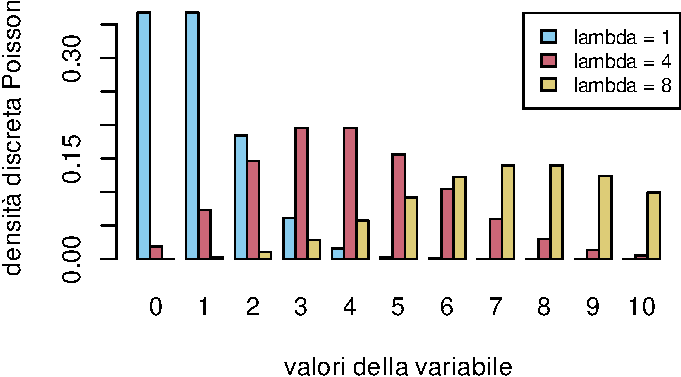
\includegraphics[keepaspectratio]{VA_generali_files/figure-pdf/unnamed-chunk-2-1.pdf}}

}

\caption{Grafico a barre della densità Poisson fino a \(k=10\), con
parametri \(\lambda=1,4,8\).}

\end{figure}%

La densità discreta permette di conoscere tutta la legge di \(X\)
(sempre nel cason in cui i possibili valori \(E\) siano un insieme
finito oppure infinito ma ``discreto''): si tratta di una semplice
conseguenza della regola della somma, e per il caso infinito, di un
passaggio al limite (appoggiandosi alla teoria di Kolmogorov per
renderlo rigoroso).

Se \(X\) assume valori in un insieme \(E\) finito oppure infinito
discreto, vale per ogni \(U \subseteq E\),
\[ P(X \in U|I) = \sum_{x \in U} P(X = x |I),\] dove la sommatoria è
intesa come serie nel caso infinito.

La probabilità che una variabile Binomiale di parametri \(n=7\),
\(p=1/6\) assuma valori pari, si ottiene ponendo \(U = \cur{0,2,4,6}\),
e pertanto vale (non indichiamo \(I\))
\[  \begin{split} P(X=0)+P(X=2)+ P(X=4)+P(X=6)  & = \sum_{k=0}^3 P(X = 2k)\\
& = \sum_{k=0}^3 {7 \choose 2k} \bra{\frac 1 3}^{2k} \bra{\frac 2 3 }^{7 - 2k},\end{split}\]
che vale circa il \(53\%\), come mostra il seguente codice R.

\begin{Shaded}
\begin{Highlighting}[]
\CommentTok{\# crea il vettore con i valori richiesti }
\NormalTok{pari }\OtherTok{\textless{}{-}} \DecValTok{2}\SpecialCharTok{*}\NormalTok{(}\DecValTok{0}\SpecialCharTok{:}\DecValTok{3}\NormalTok{)}

\CommentTok{\# calcola la densità discreta nei valori richiesti}

\NormalTok{dens\_pari }\OtherTok{\textless{}{-}} \FunctionTok{dbinom}\NormalTok{(pari, }\DecValTok{7}\NormalTok{, }\DecValTok{1}\SpecialCharTok{/}\DecValTok{6}\NormalTok{)}

\CommentTok{\# somma le densità trovate per trovare la probabilità richiesta}

\NormalTok{(prob\_pari }\OtherTok{\textless{}{-}} \FunctionTok{sum}\NormalTok{(dens\_pari))}
\end{Highlighting}
\end{Shaded}

\begin{verbatim}
[1] 0.5292638
\end{verbatim}

Possiamo anche evidenziare nel grafico a barre i valori della variabile
\(X\) che contribuiscono a determinare la probabilità richiesta (che
risulta quindi la somma delle altezze delle barre evidenziate).

\begin{Shaded}
\begin{Highlighting}[]
\CommentTok{\# usiamo la funzione dbinom() per ottenere direttamente la densità binomiale con i parametri cercati}

\NormalTok{n }\OtherTok{\textless{}{-}} \DecValTok{7}
\NormalTok{k }\OtherTok{\textless{}{-}} \DecValTok{0}\SpecialCharTok{:}\NormalTok{n}
\NormalTok{p }\OtherTok{\textless{}{-}} \DecValTok{1}\SpecialCharTok{/}\DecValTok{6}

\NormalTok{dens }\OtherTok{\textless{}{-}} \FunctionTok{dbinom}\NormalTok{(k, n, p)}

\CommentTok{\# parametri per il plot: coloriamo di rosso le probabilità relative agli esiti pari}

\NormalTok{valori }\OtherTok{\textless{}{-}} \FunctionTok{as.character}\NormalTok{(k)}
\NormalTok{colori }\OtherTok{\textless{}{-}} \FunctionTok{c}\NormalTok{(miei\_colori[}\DecValTok{2}\NormalTok{],  }\FunctionTok{rep}\NormalTok{(miei\_colori[}\DecValTok{1}\SpecialCharTok{:}\DecValTok{2}\NormalTok{], }\DecValTok{3}\NormalTok{))}


\FunctionTok{barplot}\NormalTok{( dens, }\AttributeTok{col=}\NormalTok{colori, }\AttributeTok{names.arg=}\NormalTok{valori, }\AttributeTok{ylab=}\StringTok{"probabilità"}\NormalTok{, }\AttributeTok{xlab=}\StringTok{"valore"}\NormalTok{)}
\end{Highlighting}
\end{Shaded}

\begin{figure}[H]

{\centering \pandocbounded{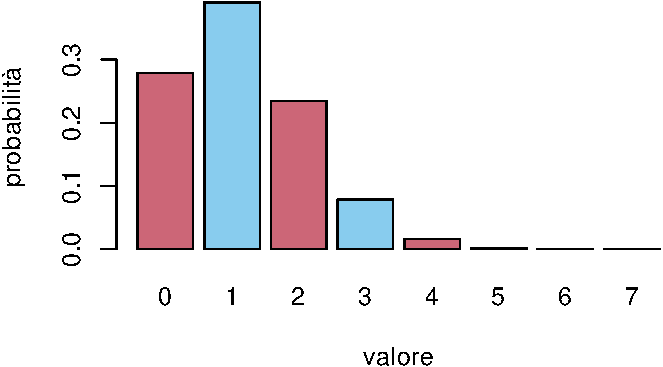
\includegraphics[keepaspectratio]{VA_generali_files/figure-pdf/unnamed-chunk-4-1.pdf}}

}

\caption{rappresentazione grafica della probabilità che una variabile
con densità binomiale di parametri \(n=7\), \(p=1/10\) assuma un valore
pari}

\end{figure}%

\subsection{Densità continua}\label{densituxe0-continua}

Un problema sorge quando si vuole trattare il caso di un infinito
``continuo'', come ad esempio un intervallo dei numeri reali.
L'interesse per questo caso è che alcune grandezze si rappresentano
meglio come un ``continuo'' di valori (si pensi alla temperatura di un
oggetto, la velocità di un mezzo, ecc.), e inoltre questo permetterebbe
l'uso di tecniche di calcolo (derivate, integrali, ecc.).

Per dare un'esempio concreto, supponiamo di voler definire una variabile
\(X\) ``uniforme'' su tutti i valori dell'intervallo \([0,1]\): ad
esempio, \(\cur{X = x}\) potrebbe rappresentare l'informazione che
un'urna contiene una frazione \(x\) di palline rosse sul totale. Si
tratta ovviamente di una idealizzazione e si può pensare come il limite
della densità discreta uniforme sugli \(n\) valori
\(\cur{1/n, 2/n, \ldots, 1}\) per \(n\) che tende ad infinito. Il
passaggio al limite però è piuttosto tecnico, quindi vorremmo
direttamente definire un analogo continuo della densità uniforme.
Notiamo tuttavia che \emph{non} possiamo definire \[ P(X = x | I) = c \]
per nessun valore \(c>0\), altrimenti sommando sugli infiniti valori
possibili, la serie diverge: \[ \sum_{x \in [0,1]} c = \infty.\] L'idea
informale è quindi che ogni alternativa \(\cur{X =x}\) ha una quantità
\emph{infinitesima} di probabilità, un po' come in una catena ogni
anello contribuisce alla massa totale. Per rendere preciso questo
concetto, introduciamo una funzione di \emph{densità continua} di
probabilità, che denoteremo ad esempio \[ p(X = x | I)\] che va intesa
come la quantità di probabilità per unità di lunghezza (allo stesso modo
come la densità di massa o la densità di carica in fisica). Dato un
intervallo \([x, x + \Delta x]\) di lunghezza \(\Delta x\) molto
piccola, si potrà approssimare
\[ P(X \in [x, x + \Delta x] | I ) \sim  p(X = x | I) \Delta x.\]

Diamo allora una definizione rigorosa.

Sia \(X\) una variabile aleatoria a valori in \(\R\) e sia
\(f: \R \to [0, \infty)\) una funzione integrabile nel senso di Riemann,
eventualmente improprio, tale che
\[ \int_{-\infty}^\infty f(x) d x = 1.\] Si dice che \(X\) ha densità
continua\footnote{o funzione di densità di probabilità, in inglese
  \textbf{probability density function}, abbreviato \emph{pdf}} \(f\)
(rispetto all'informazione \(I\)) se vale, per ogni intervallo
\((a,b) \subseteq \R\), \[ P( a < X < b | I) = \int_a^b f(x) d x,\]

Ricordando l'interpretazione dell'integrale come area sotto il grafico
di \(f\), segue che l'area sottesa dal grafico su tutta la retta reale
vale \(1\), mentre la probabilità che \(X\) assuma valori
nell'intervallo \((a,b)\) è l'area sotto il grafico ristretto
all'intervallo.

\begin{Shaded}
\begin{Highlighting}[]
\CommentTok{\# plottiamo la densità f(x) = 3/4( 1{-}x\^{}2) su ({-}1, 1) e nulla fuori dall\textquotesingle{}intervallo.}

\NormalTok{deltax }\OtherTok{\textless{}{-}} \FloatTok{0.01}
\NormalTok{x }\OtherTok{\textless{}{-}} \FunctionTok{seq}\NormalTok{(}\SpecialCharTok{{-}}\DecValTok{1}\NormalTok{, }\DecValTok{1}\NormalTok{, }\AttributeTok{by=}\NormalTok{deltax)}
\NormalTok{dens }\OtherTok{\textless{}{-}}\NormalTok{ (}\DecValTok{1}\SpecialCharTok{{-}}\NormalTok{ x}\SpecialCharTok{\^{}}\DecValTok{2}\NormalTok{)}\SpecialCharTok{*}\DecValTok{3}\SpecialCharTok{/}\DecValTok{4}


\FunctionTok{plot}\NormalTok{(x, dens, }\AttributeTok{type=}\StringTok{\textquotesingle{}l\textquotesingle{}}\NormalTok{, }\AttributeTok{xlab=}\StringTok{\textquotesingle{}valori\textquotesingle{}}\NormalTok{, }\AttributeTok{ylab=}\StringTok{\textquotesingle{}densità continua\textquotesingle{}}\NormalTok{, }\AttributeTok{lwd=}\DecValTok{3}\NormalTok{, }\AttributeTok{col=}\NormalTok{miei\_colori[}\DecValTok{2}\NormalTok{])}

\CommentTok{\# evidenziamo l\textquotesingle{}area sotto il grafico  nell\textquotesingle{}intervallo ({-}1/2, 0)}

\FunctionTok{polygon}\NormalTok{( }\FunctionTok{c}\NormalTok{(x[}\DecValTok{50}\SpecialCharTok{:}\DecValTok{100}\NormalTok{], x[}\DecValTok{100}\NormalTok{], x[}\DecValTok{50}\NormalTok{]), }\FunctionTok{c}\NormalTok{(dens[}\DecValTok{50}\SpecialCharTok{:}\DecValTok{100}\NormalTok{], }\DecValTok{0}\NormalTok{, }\DecValTok{0}\NormalTok{), }\AttributeTok{col=}\NormalTok{miei\_colori[}\DecValTok{1}\NormalTok{] )}
\end{Highlighting}
\end{Shaded}

\begin{figure}[H]

{\centering \pandocbounded{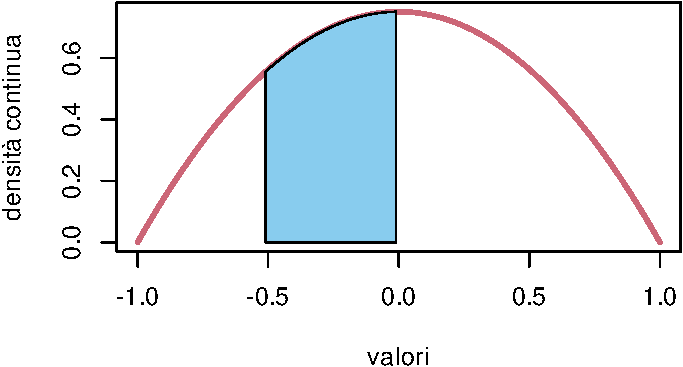
\includegraphics[keepaspectratio]{VA_generali_files/figure-pdf/unnamed-chunk-5-1.pdf}}

}

\caption{Una densità continua è tale che l'area sotto il grafico valga
\(1\), mentre la probabilità che assuma valori in un intervallo è uguale
all'area (in azzurro) sotto il grafico ristretto all'intervallo}

\end{figure}%

\begin{remark}
Nonostante il nome, non è richiesto che \(f\) sia una funzione continua
(anche se in molti casi interessanti lo è). Ad esempio può presentare
delle discontinuità a salto, che comunque non danno problemi nel calcolo
dell'integrale.
\end{remark}

Spesso si dice anche che \(X\) è una variabile aleatoria continua, per
dire che \(X\) ammette una densità continua. Si può mostrare che, se
\(X\) ammette densità continua, la funzione \(f\) è quasi del tutto
determinata (eccetto al più in pochi punti, in modo da non modificare
gli integrali). Si può quindi introdurre una notazione per identificare
tale \(f\). Il problema purtroppo è che non vi è un'unica convenzione
per indicare la densità, ad esempio in alcuni testi si trova \(f_X\), in
altri \(p_X(x)\) oppure semplicemente \(p(x)\) (usando la variabile
matematica, non aleatoria, \(x\) per ricordare che è la densità della
variabile aleatoria \(X\)). Inoltre in molte notazioni non è indicata
l'informazione \(I\) (spesso perché e fissata). In questo caso conviene
sempre chiedere precisazioni su una notazione, se non è chiara. Noi
adotteremo la seguente notazione: \[ p(X = x |I), \] dove l'unica
differenza è la \(p\) minuscola rispetto alla \(P\) maiuscola di
probabilità. Pertanto la formula che \emph{definisce} la densità di
\(X\) si riscrive come \[ P( a< X< b|I) = \int_a^b p(X=x|I) d x.\]

Una variabile \(X\) che ammette densità continua \(p(X=x|I)\)
necessariamente è tale che \(P(X=x|I) = 0\) per ogni \(x \in \R\) (ossia
ha densità discreta nulla), perché prendendo un intervallo \((a,b)\)
contenente \(x\), si ha per monotonia
\[ P(X = x | I) \le P(a<X<b | I ) = \int_a^b p(X=x|I) d x,\] e al
tendere di \(a, b \to x\) l'integrale tende a zero.

\begin{remark}
L'analogia con il caso discreto è quindi che l'integrale sostituisce la
somma, tuttavia vale la pena di notare che, dovendo attribuire una
``unità di misura'' alla densità di probabilità, essa sarebbe
{[}probabilità{]}/{[}unità di misura di \(X\){]} (ad esempio metri se
\(X\) rappresenta una lunghezza in metri), mentre la probabilità
``infinitesima'' sarebbe il termine formale \(p(X=x|I)dx\).
\end{remark}

Vediamo due esempi.

Dato un intervallo \([a,b] \subseteq \R\), si dice che \(X\) è una
variabile uniforme (continua) su \([a,b]\) se ammette densità continua
\emph{costante} sull'intervallo \([a,b]\) e \emph{nulla} al di fuori di
esso. Pertanto, dovendo avere area unitaria, si deduce che
\[ p(X=x| \text{uniforme su $[a,b]$}) = \begin{cases} \frac 1 {b-a} & \text{se $x \in [a,b] $}\\ 0 & \text{altrimenti} \end{cases} \]
In particolare, se \(b-a<1\) la densità assume valori maggiori di \(1\)
(questo fatto è ovviamente possibile, perché la condizione di essere
compresa tra \(0\) e \(1\) riguarda la probabilità, non la densità).

\begin{Shaded}
\begin{Highlighting}[]
\CommentTok{\#creiamo un grafico vuoto}

\FunctionTok{plot}\NormalTok{(}\ConstantTok{NULL}\NormalTok{, }\AttributeTok{xlim=}\FunctionTok{c}\NormalTok{(}\SpecialCharTok{{-}}\DecValTok{1}\NormalTok{,}\DecValTok{1}\NormalTok{), }\AttributeTok{ylim=}\FunctionTok{c}\NormalTok{(}\DecValTok{0}\NormalTok{,}\DecValTok{3}\NormalTok{), }\AttributeTok{xlab=}\StringTok{\textquotesingle{}valori\textquotesingle{}}\NormalTok{, }\AttributeTok{ylab=}\StringTok{\textquotesingle{}densità continua\textquotesingle{}}\NormalTok{)}

\CommentTok{\# aggiungiamo i segmenti con il comando lines}

\FunctionTok{lines}\NormalTok{( }\AttributeTok{x=}\FunctionTok{c}\NormalTok{(}\SpecialCharTok{{-}}\DecValTok{1}\NormalTok{, }\DecValTok{0}\NormalTok{), }\AttributeTok{y=}\FunctionTok{c}\NormalTok{(}\DecValTok{0}\NormalTok{,}\DecValTok{0}\NormalTok{), }\AttributeTok{col=}\NormalTok{miei\_colori[}\DecValTok{2}\NormalTok{], }\AttributeTok{lwd=}\DecValTok{3}\NormalTok{)}
\FunctionTok{lines}\NormalTok{( }\AttributeTok{x=}\FunctionTok{c}\NormalTok{(}\DecValTok{0}\NormalTok{, }\DecValTok{1}\SpecialCharTok{/}\DecValTok{3}\NormalTok{), }\AttributeTok{y=}\FunctionTok{c}\NormalTok{(}\DecValTok{3}\NormalTok{,}\DecValTok{3}\NormalTok{), }\AttributeTok{col=}\NormalTok{miei\_colori[}\DecValTok{2}\NormalTok{], }\AttributeTok{lwd=}\DecValTok{3}\NormalTok{)}
\FunctionTok{lines}\NormalTok{( }\AttributeTok{x=}\FunctionTok{c}\NormalTok{(}\DecValTok{1}\SpecialCharTok{/}\DecValTok{3}\NormalTok{, }\DecValTok{1}\NormalTok{), }\AttributeTok{y=}\FunctionTok{c}\NormalTok{(}\DecValTok{0}\NormalTok{,}\DecValTok{0}\NormalTok{), }\AttributeTok{col=}\NormalTok{miei\_colori[}\DecValTok{2}\NormalTok{], }\AttributeTok{lwd=}\DecValTok{3}\NormalTok{)}

\CommentTok{\# aggiungiamo dei segmenti tratteggiati per evidenziare la discontinuità}

\FunctionTok{lines}\NormalTok{( }\AttributeTok{x=}\FunctionTok{c}\NormalTok{(}\DecValTok{1}\SpecialCharTok{/}\DecValTok{3}\NormalTok{, }\DecValTok{1}\SpecialCharTok{/}\DecValTok{3}\NormalTok{), }\AttributeTok{y=}\FunctionTok{c}\NormalTok{(}\DecValTok{0}\NormalTok{,}\DecValTok{3}\NormalTok{), }\AttributeTok{type=}\StringTok{\textquotesingle{}l\textquotesingle{}}\NormalTok{, }\AttributeTok{lty=}\StringTok{\textquotesingle{}dashed\textquotesingle{}}\NormalTok{, }\AttributeTok{col=}\NormalTok{miei\_colori[}\DecValTok{2}\NormalTok{])}
\FunctionTok{lines}\NormalTok{( }\AttributeTok{x=}\FunctionTok{c}\NormalTok{(}\DecValTok{0}\NormalTok{, }\DecValTok{0}\NormalTok{), }\AttributeTok{y=}\FunctionTok{c}\NormalTok{(}\DecValTok{0}\NormalTok{,}\DecValTok{3}\NormalTok{), }\AttributeTok{type=}\StringTok{\textquotesingle{}l\textquotesingle{}}\NormalTok{, }\AttributeTok{lty=}\StringTok{\textquotesingle{}dashed\textquotesingle{}}\NormalTok{, }\AttributeTok{col=}\NormalTok{miei\_colori[}\DecValTok{2}\NormalTok{])}
\end{Highlighting}
\end{Shaded}

\begin{figure}[H]

{\centering \pandocbounded{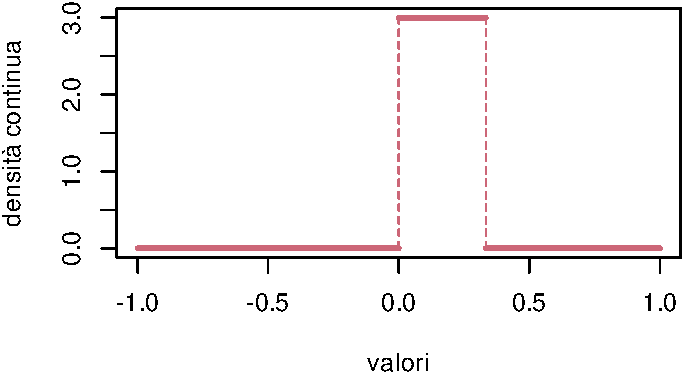
\includegraphics[keepaspectratio]{VA_generali_files/figure-pdf/unnamed-chunk-6-1.pdf}}

}

\caption{densità uniforme sull'intervallo \([0,1/3]\).}

\end{figure}%

Dato un parametro \(\lambda>0\), si dice che \(X\) a valori in \(\R\) è
una variabile con legge esponenziale (con parametro \(\lambda\)) se
ammette densità continua proporzionale a \(e^{-\lambda x}\) se
\(x \ge 0\) e \emph{nulla} per \(x<0\) (quindi a tutti gli effetti la
variabile assume valori positivi). Pertanto, dovendo avere area
unitaria, si deduce che
\[ p(X=x| \text{Exp}(\lambda) ) = \begin{cases} \lambda e^{-\lambda x} & \text{se $x \ge 0$}\\
0 & \text{altrimenti.}
\end{cases} \] In particolare, maggiore è \(\lambda\), maggiore è la
densità vicino a \(x=0\) (vedere i grafici) e di conseguenza maggiore la
probabilità che \(X\) assuma valori piccoli. Vedremo in un senso preciso
che \(X\) vale circa (in media) \(1/\lambda\).

\begin{Shaded}
\begin{Highlighting}[]
\CommentTok{\#creiamo un grafico vuoto}

\FunctionTok{plot}\NormalTok{(}\ConstantTok{NULL}\NormalTok{, }\AttributeTok{xlim=}\FunctionTok{c}\NormalTok{(}\DecValTok{0}\NormalTok{,}\DecValTok{4}\NormalTok{), }\AttributeTok{ylim=}\FunctionTok{c}\NormalTok{(}\DecValTok{0}\NormalTok{,}\DecValTok{2}\NormalTok{), }\AttributeTok{xlab=}\StringTok{\textquotesingle{}valori\textquotesingle{}}\NormalTok{, }\AttributeTok{ylab=}\StringTok{\textquotesingle{}densità continua\textquotesingle{}}\NormalTok{)}

\CommentTok{\# aggiungiamo le densità con il comando lines() e la funzione dexp() per calcolare la densità esponenziale}

\NormalTok{deltax }\OtherTok{\textless{}{-}} \FloatTok{0.01}
\NormalTok{x }\OtherTok{\textless{}{-}} \FunctionTok{seq}\NormalTok{(}\DecValTok{0}\NormalTok{, }\DecValTok{4}\NormalTok{, }\AttributeTok{by=}\NormalTok{deltax)}

\FunctionTok{lines}\NormalTok{( x, }\FunctionTok{dexp}\NormalTok{(x, }\AttributeTok{rate=}\DecValTok{1}\SpecialCharTok{/}\DecValTok{2}\NormalTok{), }\AttributeTok{col=}\NormalTok{miei\_colori[}\DecValTok{1}\NormalTok{], }\AttributeTok{lwd=}\DecValTok{3}\NormalTok{)}
\FunctionTok{lines}\NormalTok{( x, }\FunctionTok{dexp}\NormalTok{(x, }\AttributeTok{rate=}\DecValTok{1}\NormalTok{), }\AttributeTok{col=}\NormalTok{miei\_colori[}\DecValTok{2}\NormalTok{], }\AttributeTok{lwd=}\DecValTok{3}\NormalTok{)}
\FunctionTok{lines}\NormalTok{( x, }\FunctionTok{dexp}\NormalTok{(x, }\AttributeTok{rate=}\DecValTok{2}\NormalTok{),  }\AttributeTok{col=}\NormalTok{miei\_colori[}\DecValTok{3}\NormalTok{], }\AttributeTok{lwd=}\DecValTok{3}\NormalTok{)}

\CommentTok{\# linea tratteggiata per evidenzare la discontinuità in 0}
\FunctionTok{lines}\NormalTok{( }\FunctionTok{c}\NormalTok{(}\DecValTok{0}\NormalTok{,}\DecValTok{0}\NormalTok{), }\FunctionTok{c}\NormalTok{(}\DecValTok{0}\NormalTok{,}\DecValTok{2}\NormalTok{), }\AttributeTok{lty=}\StringTok{\textquotesingle{}dashed\textquotesingle{}}\NormalTok{, }\AttributeTok{col=}\StringTok{\textquotesingle{}gray\textquotesingle{}}\NormalTok{)}


\CommentTok{\# legenda}

\FunctionTok{legend}\NormalTok{(}\StringTok{\textquotesingle{}topright\textquotesingle{}}\NormalTok{, }\AttributeTok{fill=}\NormalTok{miei\_colori[}\DecValTok{1}\SpecialCharTok{:}\DecValTok{3}\NormalTok{], }\AttributeTok{legend=}\FunctionTok{c}\NormalTok{(}\StringTok{"lambda = 1/2"}\NormalTok{, }\StringTok{"lambda = 1"}\NormalTok{, }\StringTok{"lambda = 2"}\NormalTok{), }\AttributeTok{cex=}\FloatTok{0.8}\NormalTok{)}
\end{Highlighting}
\end{Shaded}

\begin{figure}[H]

{\centering \pandocbounded{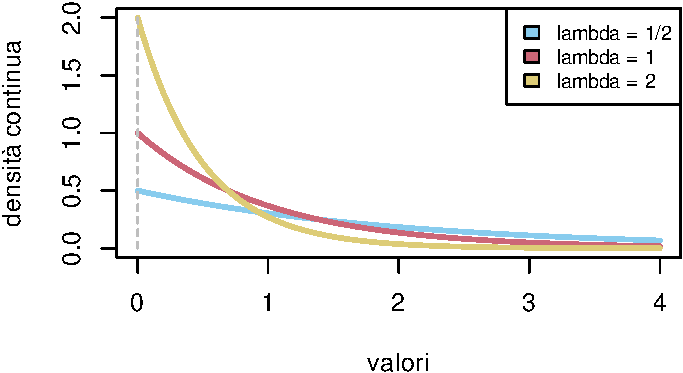
\includegraphics[keepaspectratio]{VA_generali_files/figure-pdf/unnamed-chunk-7-1.pdf}}

}

\caption{densità esponenziale per \(\lambda = 1/2, 1, 2\)}

\end{figure}%

Quanto introdotto nel caso di variabili a valori in \(\R\) si estende al
caso di variabili \emph{vettoriali}, ossia a valori in uno spazio
\(\R^d\) (ad esempio a valori nel piano se \(d=2\)), purché si faccia
utilizzo dell'integrazione in più variabili. Nel corso ci soffermeremo
solamente su alcuni casi speciali di leggi di variabili vettoriali (in
particolare le variabili gaussiane), ma possiamodare qui una definizione
generale di densità continua, analoga al caso reale \(d=1\). Non
chiederemo comunque mai negli esercizi di calcolare integrali in più
variabili.

Sia \(X\) una variabile aleatoria a valori in \(\R^d\) e sia
\(f: \R^d \to [0, \infty)\) una funzione integrabile (in più variabili)
tale che
\[\int_{\R^d} f =  \int_{-\infty}^\infty d x_1 \ldots \int_{-\infty}^\infty dx_d \, f(x_1, \ldots, x_d) = 1.\]
Si dice che \(X\) ha densità continua \(f\) (rispetto all'informazione
\(I\)) se vale, per ogni ``rettangolo''
\[ U = (a_1,b_1) \times \ldots \times (a_d,b_d) \subseteq \R^d,\]
\[ P( X \in U | I) = \int_U f =  \int_{a_1}^{b_1} d x_1 \ldots \int_{a_d}^{b_d} dx_d \, f(x_1, \ldots, x_d).\]

Anche in questo caso indicheremo con \[p(X = x | I)\] la densità
continua di \(X\), con \(x \in \R^d\) (anch'essa è determinata a meno di
modificazioni che non cambiano gli integrali in più variabili). Stavolta
però, per guidare l'intuizione, osserviamo che l'unità di misura
asociata alla densità è {[}probabilità{]}/{[}volume{]}, se ciascuna
coordinata rappresenta una lunghezza (altrimenti un prodotto opportuno
delle unità di misura di ciascuna coordinata).

\subsection{Esercizi}\label{esercizi-10}

Usando il comando R \texttt{dbinom()} calcolare la probabilità che una
variabile aleatoria con densità binomiale di parametri \((15, 1/2)\)
assuma valori pari. Ripetere con i parametri \((16, 1/2)\) e
\((17, 1/2)\), \((18, 1/2)\). Cosa notate?

Sia \(X\) una variabile aleatoria con densità continua esponenziale di
parametro \(\lambda = 3\). Calcolare la probabilità dell'evento
\[ \cur{ |X-1| <1/2} \cup \cur{ X^2 >9},\] sia analiticamente sia
numericamente con opportuni comandi \(R\) (approssimare eventualmente
gli integrali con una somma finita).

Sia \(X\) una variabile con densità continua uniforme su
\([a,b] \subseteq \R\), rispetto ad una informazione nota \(I\). Si
supponga di osservare che \(X \in [c,d]\), dove
\([c,d ]\subseteq [a,b]\). Come cambia la densità di \(X\)?

\section{Composizione tramite funzione}\label{sec-composizione}

Sia data \(X\) una variabile aleatoria a valori in \(E\) e sia
\(g: E \to F\) una funzione. Per definire la variabile composta
\(g(X)\), è sufficiente descrivere il suo sistema di alternative
associato. Per ogni \(z \in F\), se vale \(g(X) = z\) significa che
\(X\) assume uno dei possibili valori \(x\in E\) tali che \(g(x) = z\).
Tale inseme di valori \(x\) è detto \emph{immagine inversa} di \(z\)
tramite \(g\), e si indica \(g^{-1}(z)\). Se \(g\) è invertibile,
\(g^{-1}(z)\) consiste di un solo valore, ma in generale individua un
sottoinsieme (possibilmente anche vuoto) di \(E\).

Se \(X\) è una variabile aleatoria a valori in \(E\) e \(g: E \to F\) è
una funzione, si una definisce la variabile aleatoria \(g(X)\) a valori
in \(F\) tramite il sistema di alternative, per \(z \in F\),
\[ \cur{ g(X) = z} =  \cur{X \in g^{-1}(z)}.\]

Per verificare che la famiglia così definita sia un sistema di
alternative, basta notare che, al variare di \(z \in F\), gli insiemi
\(g^{-1}(z)\) sono una partizione di \(E\): ogni possibile valore
\(x \in E\) appartiene ad uno e uno solo di tali insiemi, pertanto una e
una sola tra le affermazioni \(\cur{g(X) = z}\) è vera.

Si lancia un dado a sei facce e si pone \(X \in E= \cur{1,2,3,4,5,6}\)
l'esito del lancio. Posta \(g(x)\) la funzione che vale \(1\) se \(x\) è
dispari, \(0\) altrimenti, la variabile \(g(X)\) a valori in
\(F=\cur{0,1}\) indica se l'esito del lancio è dispari. In particolare,
prima di sapere l'esito del lancio, ha densità discreta uniforme (oppure
Bernoulli di parametro \(1/2\)), perché
\[ \cur{ g(X)  =1 } = \cur{ X \in g^{-1}(1)} = \cur{ X = 1 \text{oppure} X=3 \text{oppure} X =5}.\]
che ha probabilità \(1/2\).

L'esempio sopra ci indica un metodo per calcolare la densità discreta di
\(g(X)\) (qualora abbia senso farlo, ossia l'insieme dei possibili
valori di \(g(X)\) è finito o infinito ma discreto). Per ogni
\(z \in F\), si tratta di calcolare
\[ \cur{ g(X) = z } = \cur{X \in g^{-1}(z)}.\] A questo punto, se anche
\(X\) ha densità discreta, basterà sommare sui valori
\(x \in g^{-1}(z)\), ossia gli \(x \in E\) tali che \(g(x) = z\) e si
ottiene \[ P( g(X) = z |I)  = \sum_{x \in g^{-1}(z)} P(X = x | I). \]
Altrimenti, nel caso in cui \(X\) abbia densità continua, bisogna
sostituire la somma con un integrale (o più in generale con una somma di
integrali) sull'insieme \(g^{-1}(z)\):
\[ P(g(X) = z | I) = \int_{g^{-1}(z)} p(X=x|I) dx.\]

Sia \(X\) una variabile continua con densità esponenziale di parametro
\(\lambda=1\) (rispetto ad una informazione \(I\)). Si consideri la
funzione \(g(x)\) che vale \(1\) se \(X\) è minore di \(1\) oppure
maggiore di \(2\), e si ponga \(g(x)=0\) altrimenti. Allora la variabile
\(g(X)\) assume solo i valori \(\cur{0,1}\), e quindi è discreta. Per
calcolarne la densità discreta basta determinare
\[\begin{split} P( g(X) = 1 | I) &= P( X \in g^{-1}(1)|I) = P(X<1 \text{ oppure  } X >2 |I) \\
& =  P(X<1|I) + P(X>2|I) =\int_0^1 e^{-x}dx + \int_2^\infty e^{-x }dx \\
& = 1-e^{-1} + e^{-2}
\end{split}
\]

\begin{Shaded}
\begin{Highlighting}[]
\CommentTok{\# plottiamo la densità esponenziale }

\NormalTok{deltax }\OtherTok{\textless{}{-}} \FloatTok{0.01}
\NormalTok{x }\OtherTok{\textless{}{-}} \FunctionTok{seq}\NormalTok{(}\DecValTok{0}\NormalTok{, }\DecValTok{5}\NormalTok{, }\AttributeTok{by=}\NormalTok{deltax)}
\NormalTok{dens }\OtherTok{\textless{}{-}} \FunctionTok{dexp}\NormalTok{(x)}


\FunctionTok{plot}\NormalTok{(x, dens, }\AttributeTok{type=}\StringTok{\textquotesingle{}l\textquotesingle{}}\NormalTok{, }\AttributeTok{xlab=}\StringTok{\textquotesingle{}valori\textquotesingle{}}\NormalTok{, }\AttributeTok{ylab=}\StringTok{\textquotesingle{}densità continua\textquotesingle{}}\NormalTok{, }\AttributeTok{lwd=}\DecValTok{3}\NormalTok{, }\AttributeTok{col=}\NormalTok{miei\_colori[}\DecValTok{2}\NormalTok{])}

\CommentTok{\# evidenziamo l\textquotesingle{}area sotto il grafico  nell\textquotesingle{}intervallo (0, 1) e nell\textquotesingle{}intervallo (2, 5) (per ragioni di spazio non possiamo andare oltre)}

\FunctionTok{polygon}\NormalTok{( }\FunctionTok{c}\NormalTok{(x[x}\SpecialCharTok{\textless{}}\DecValTok{1}\NormalTok{], x[x}\SpecialCharTok{==}\DecValTok{1}\NormalTok{], x[}\DecValTok{1}\NormalTok{]), }\FunctionTok{c}\NormalTok{(dens[x}\SpecialCharTok{\textless{}}\DecValTok{1}\NormalTok{], }\DecValTok{0}\NormalTok{, }\DecValTok{0}\NormalTok{), }\AttributeTok{col=}\NormalTok{miei\_colori[}\DecValTok{1}\NormalTok{])}

\FunctionTok{polygon}\NormalTok{( }\FunctionTok{c}\NormalTok{(x[x}\SpecialCharTok{\textgreater{}=}\DecValTok{2}\NormalTok{], x[x}\SpecialCharTok{==}\DecValTok{5}\NormalTok{], x[x}\SpecialCharTok{==}\DecValTok{2}\NormalTok{]), }\FunctionTok{c}\NormalTok{(dens[x}\SpecialCharTok{\textgreater{}=}\DecValTok{2}\NormalTok{], }\DecValTok{0}\NormalTok{, }\DecValTok{0}\NormalTok{), }\AttributeTok{col=}\NormalTok{miei\_colori[}\DecValTok{1}\NormalTok{])}
\end{Highlighting}
\end{Shaded}

\begin{figure}[H]

{\centering \pandocbounded{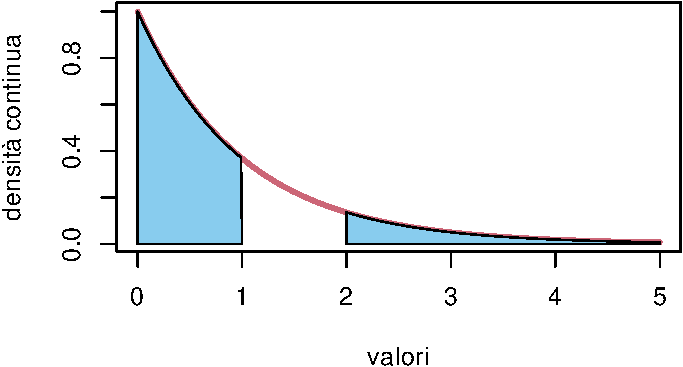
\includegraphics[keepaspectratio]{VA_generali_files/figure-pdf/unnamed-chunk-8-1.pdf}}

}

\caption{La probabilità di \(\cur{ g(X) =1 }\) corrisponde all'area del
sottografico della densità esponeziale negli intervalli
\(g^{-1}(1) = (0,1) \cup (2, \infty)\).}

\end{figure}%

\begin{Shaded}
\begin{Highlighting}[]
\CommentTok{\# calcoliamo infine l\textquotesingle{}area numericamente}


\NormalTok{((}\FunctionTok{sum}\NormalTok{( dens[x}\SpecialCharTok{\textless{}}\DecValTok{1}\NormalTok{])}\SpecialCharTok{+} \FunctionTok{sum}\NormalTok{( dens[x}\SpecialCharTok{\textgreater{}}\DecValTok{2}\NormalTok{]))}\SpecialCharTok{*}\NormalTok{deltax)}
\end{Highlighting}
\end{Shaded}

\begin{verbatim}
[1] 0.7632419
\end{verbatim}

\begin{Shaded}
\begin{Highlighting}[]
\CommentTok{\# e la confrontiamola con quella teorica}

\NormalTok{(}\AttributeTok{prob\_teorica =} \DecValTok{1}\SpecialCharTok{{-}}\FunctionTok{exp}\NormalTok{(}\SpecialCharTok{{-}}\DecValTok{1}\NormalTok{)}\SpecialCharTok{+}\FunctionTok{exp}\NormalTok{(}\SpecialCharTok{{-}}\DecValTok{2}\NormalTok{))}
\end{Highlighting}
\end{Shaded}

\begin{verbatim}
[1] 0.7674558
\end{verbatim}

Quando accade invece che, se \(X\) ha densità continua, anche \(g(X)\)
ammette densità continua? Sicuramente \(g\) deve assumere un infinità
continua di valori, tuttavia non è sufficiente, come mostra il seguente
esempio.

Sia \(X\) una varibile continua uniforme nell'intervallo \([-1,1]\) e
sia \(g: \R \to \R\) definita a tratti
\[ g(x) = \begin{cases} x & \text{se $x \ge 0$,}\\
                        0 & text{altrimenti.}\end{cases}\]

\begin{Shaded}
\begin{Highlighting}[]
\NormalTok{x }\OtherTok{\textless{}{-}} \FunctionTok{seq}\NormalTok{(}\SpecialCharTok{{-}}\DecValTok{2}\NormalTok{, }\DecValTok{2}\NormalTok{)}

\FunctionTok{plot}\NormalTok{(}\ConstantTok{NULL}\NormalTok{, }\AttributeTok{xlim=}\FunctionTok{c}\NormalTok{(}\SpecialCharTok{{-}}\DecValTok{2}\NormalTok{,}\DecValTok{2}\NormalTok{), }\AttributeTok{ylim=}\FunctionTok{c}\NormalTok{(}\DecValTok{0}\NormalTok{,}\DecValTok{2}\NormalTok{), }\AttributeTok{xlab=}\StringTok{\textquotesingle{}valori\textquotesingle{}}\NormalTok{, }\AttributeTok{ylab=}\StringTok{\textquotesingle{}densità e g(x)\textquotesingle{}}\NormalTok{)}

\CommentTok{\# plottiamo la densità uniforme}

\FunctionTok{lines}\NormalTok{( }\AttributeTok{x=}\FunctionTok{c}\NormalTok{(}\SpecialCharTok{{-}}\DecValTok{2}\NormalTok{, }\SpecialCharTok{{-}}\DecValTok{1}\NormalTok{), }\AttributeTok{y=}\FunctionTok{c}\NormalTok{(}\DecValTok{0}\NormalTok{,}\DecValTok{0}\NormalTok{), }\AttributeTok{lwd=}\DecValTok{3}\NormalTok{, }\AttributeTok{col=}\NormalTok{miei\_colori[}\DecValTok{2}\NormalTok{])}
\FunctionTok{lines}\NormalTok{( }\AttributeTok{x=}\FunctionTok{c}\NormalTok{(}\SpecialCharTok{{-}}\DecValTok{1}\NormalTok{, }\DecValTok{1}\NormalTok{), }\AttributeTok{y=}\FunctionTok{c}\NormalTok{(}\DecValTok{1}\SpecialCharTok{/}\DecValTok{2}\NormalTok{,}\DecValTok{1}\SpecialCharTok{/}\DecValTok{2}\NormalTok{), }\AttributeTok{lwd=}\DecValTok{3}\NormalTok{, }\AttributeTok{col=}\NormalTok{miei\_colori[}\DecValTok{2}\NormalTok{])}
\FunctionTok{lines}\NormalTok{( }\AttributeTok{x=}\FunctionTok{c}\NormalTok{(}\DecValTok{1}\NormalTok{, }\DecValTok{2}\NormalTok{), }\AttributeTok{y=}\FunctionTok{c}\NormalTok{(}\DecValTok{0}\NormalTok{,}\DecValTok{0}\NormalTok{), }\AttributeTok{lwd=}\DecValTok{3}\NormalTok{, }\AttributeTok{col=}\NormalTok{miei\_colori[}\DecValTok{2}\NormalTok{])}

\FunctionTok{lines}\NormalTok{( }\AttributeTok{x=}\FunctionTok{c}\NormalTok{(}\DecValTok{1}\NormalTok{, }\DecValTok{1}\NormalTok{), }\AttributeTok{y=}\FunctionTok{c}\NormalTok{(}\DecValTok{0}\NormalTok{,}\DecValTok{1}\SpecialCharTok{/}\DecValTok{2}\NormalTok{), }\AttributeTok{type=}\StringTok{\textquotesingle{}l\textquotesingle{}}\NormalTok{, }\AttributeTok{lty=}\StringTok{\textquotesingle{}dashed\textquotesingle{}}\NormalTok{, }\AttributeTok{col=}\NormalTok{miei\_colori[}\DecValTok{2}\NormalTok{])}
\FunctionTok{lines}\NormalTok{( }\AttributeTok{x=}\FunctionTok{c}\NormalTok{(}\SpecialCharTok{{-}}\DecValTok{1}\NormalTok{, }\SpecialCharTok{{-}}\DecValTok{1}\NormalTok{), }\AttributeTok{y=}\FunctionTok{c}\NormalTok{(}\DecValTok{0}\NormalTok{,}\DecValTok{1}\SpecialCharTok{/}\DecValTok{2}\NormalTok{), }\AttributeTok{type=}\StringTok{\textquotesingle{}l\textquotesingle{}}\NormalTok{, }\AttributeTok{lty=}\StringTok{\textquotesingle{}dashed\textquotesingle{}}\NormalTok{, }\AttributeTok{col=}\NormalTok{miei\_colori[}\DecValTok{2}\NormalTok{])}


\CommentTok{\# evidenziamo l\textquotesingle{}area che viene mandata da g nel valore 0}

\FunctionTok{polygon}\NormalTok{( }\FunctionTok{c}\NormalTok{(}\DecValTok{0}\NormalTok{,}\DecValTok{0}\NormalTok{,}\SpecialCharTok{{-}}\DecValTok{1}\NormalTok{,}\SpecialCharTok{{-}}\DecValTok{1}\NormalTok{), }\FunctionTok{c}\NormalTok{(}\DecValTok{0}\NormalTok{,.}\DecValTok{5}\NormalTok{,.}\DecValTok{5}\NormalTok{,}\DecValTok{0}\NormalTok{), }\AttributeTok{col=}\NormalTok{miei\_colori[}\DecValTok{1}\NormalTok{])}

\CommentTok{\# plottiamo il grafico di g(x)}

\FunctionTok{lines}\NormalTok{( }\AttributeTok{x=}\FunctionTok{c}\NormalTok{(}\SpecialCharTok{{-}}\DecValTok{2}\NormalTok{,}\DecValTok{0}\NormalTok{), }\AttributeTok{y=}\FunctionTok{c}\NormalTok{(}\DecValTok{0}\NormalTok{,}\DecValTok{0}\NormalTok{), }\AttributeTok{col=}\NormalTok{miei\_colori[}\DecValTok{3}\NormalTok{], }\AttributeTok{lwd=}\DecValTok{3}\NormalTok{)}
\FunctionTok{lines}\NormalTok{( }\AttributeTok{x=}\FunctionTok{c}\NormalTok{(}\DecValTok{0}\NormalTok{,}\DecValTok{2}\NormalTok{), }\AttributeTok{y=}\FunctionTok{c}\NormalTok{(}\DecValTok{0}\NormalTok{,}\DecValTok{2}\NormalTok{), }\AttributeTok{col=}\NormalTok{miei\_colori[}\DecValTok{3}\NormalTok{], }\AttributeTok{lwd=}\DecValTok{3}\NormalTok{)}
\end{Highlighting}
\end{Shaded}

\begin{figure}[H]

{\centering \pandocbounded{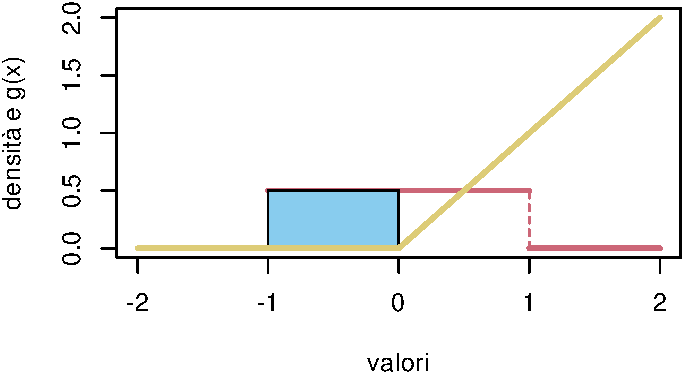
\includegraphics[keepaspectratio]{VA_generali_files/figure-pdf/unnamed-chunk-9-1.pdf}}

}

\caption{grafico della densità di \(X\) e della funzione \(g(x)\), la
probabilità corrispondente all'area in rosso viene assegnata al valore
\(0\) da \(g\)}

\end{figure}%

Allora \(g(X)\) non può essere una variabile continua, perché
\(g(X) = 0\) se e solo se \(X \in [-1,0]\) che ha probabilità \(1/2\).

Riflettendo su questo esempio, si capisce che il problema sono le
regioni in cui il grafico di \(g\) è piatto, ossia \(g'(x)=0\). In
effetti questo è l'unico ostacolo (assumendo che \(g\) sia abbastanza
regolare) a dedurre che \(g(X)\) ammette densità. Vale infatti la
seguente formula di cambio di variabile.

Sia \(X\) una variabile aleatoria a valori in \(\R\), con densità
continua \(p(X=x|I)\). Sia \(g: \R \to \R\) una funzione invertibile,
derivabile, con derivata continua e mai nulla \(g'(x)\neq 0\). Allora
\(g(X)\) ammmette densità continua e vale
\[ p(g(X) = z | I) = p( X  = g^{-1}(z) |I) \cdot\frac{1}{|g'(g^{-1}(z))|} \]

Osserviamo che il primo dei due termini a destra è piuttosto intuitivo:
si valuta la densità nell'unico punto \(x = g^{-1}(z)\) che viene
mandato da \(g\) in \(z\). Il secondo termine invece si spiega
ricordando che la densità continua ha l'unità di misura
{[}probabilità{]}/{[}lunghezza{]} e quindi ad esempio se \(X\) è
espressa in metri e \(g\) è un cambio di unità di misura (ad esempio da
metri a kilometri), \(g' = dg/dx\) ha l'unità di misura {[}Km{]}/{[}m{]}
e quindi la densità di \(g(X)\) ha l'unità di misura corretta. Inoltre
osserviamo che essendo \(g'\) a denominatore ritroviamo esattamente il
fatto che le regioni ``piatte'' o quasi piatte del grafico di \(g\)
(ossia con \(g'\) piccola) danno un contributo grande alla densità di
\(g(X)\), e nel limite \(g'=0\) si esce dal caso di densità continua.
Notiamo infine che il valore assoluto \(|g'|\) evita (giustamente)
densità negative.

\begin{proof}
La dimostrazione della formula sopra segue direttamente da un cambio di
variabile nell'integrale. Supponiamo che \(g'(x)>0\) per ogni
\(x \in \R\), ossia che \(g\) sia crescente (l'altro caso è analogo).
Dato un intervallo \([a,b]\), si ha (sottointendiamo \(I\))
\[\begin{split} P( a < g(X) < b ) &= P( g^{-1}(a) < X < g^{-1}(b))\\
& = \int_{g^{-1}(a)}^{g^{-1}(b)} p(X = x) dx \\
& \text{[posto $g(x) = z$]} \int_a^b p(X = g^{-1}(z)) (g^{-1})'(z) d z
\end{split}\] e la conclusione regue ricordando la formula per la
derivata della funzione inversa:
\[ (g^{-1})'(z) = \frac{1}{|g'(g^{-1}(z))|}.\]
\end{proof}

Consideriamo una variabile \(X\) con densità esponenziale di parametro
\(\lambda\) e sia \(g(x) = a x\), dove \(a>0\) è un altro parametro
(noto). Allora si trova \(g'(x) = a\), \(g^{-1}(z) = z/a\) e quindi la
densità di \(g(X) = aX\) è
\[ p( aX = z ) = p(X = z/a) \frac{1}{a} = \begin{cases} \frac{\lambda}{a} e^{-(\lambda/a) z} & \text{per $z \ge 0$,}\\
0 & \text{altrimenti.}
\end{cases}\] e riconosciamo quindi una densità esponenziale di
parametro modificato \(\lambda/a\).

Più in generale, se \(X\) assume con probabilità \(1\) valori in un
intervallo \(E \subseteq \R\) e \(g:E \to \R\) è tale che si può
decomporre \(E\) in una unione finita di intervalli a due a due
disgiunti in cui, all'interno di ciascun intervallo, \(g\) sia
invertibile, derivabile con derivata continua e mai nulla
\(g'(x) \neq 0\). Allora \(g(X)\) ammette densità continua
\[ p(g(X) = z | I ) = \sum_{ x \in g^{-1}(z)} p( X =x  | I ) \cdot \frac{1}{|g'(x)|}.\]
Notiamo che questa formula vale in tutti i valori \(z \in g(E)\) eccetto
al più quelli che sono immagine tramite \(g\) di un estremo degli
intervalli (dove la derivata \(g'\) potrebbe essere nulla oppure proprio
non esistere).

Consideriamo una variabile \(X\) con densità esponenziale di parametro
\(1\) e sia \(g(x) =\log(x)\), che non è definita su tutto \(\R\), ma
essendo \(P(X \le 0) = 0\), possiamo ridurci a \(E = (0, \infty)\), dove
risulta invertibile con derivata \(g^{-1}(z)= e^z\) e derivabile con
derivata \(\log'(x) = 1/x\) non nulla. Troviamo quindi la densità di
\(g(X) = \log(X)\), per \(z \in \R\),
\[ p( \log(X) = z ) = p( x = e^z) e^z = e^{-e^z + z}.\]

Sia \(X\) una variabile continua con densità uniforme sull'intervallo
\([-1,1]\) e sia \(g(x)= x^2\). In questo caso possiamo decomporre
l'intervallo \(E = [-1,1]\) in nei due intervalli \([-1,0]\) e \((0,1]\)
disgiunti, in cui \(g(x)\) è invertibile e si trova, per
\(z \in [0,1]\), \(g^{-1}(z)=\pm\sqrt{z}\) con il segno determinato
dall'intervallo che consideriamo. La funzione \(g\) è derivabile
ovunque, ma la derivata \$g'(x)= 2x \$ è nulla in \(0\). Dovremo quindi
escludere \(g(0) = 0\) dalla formula per la densità (altrimenti si trova
un contributo che possiamo intepretare come \(1/0 = \infty\)).
Applicando quindi la formula generalizzata, vale per
\(z \in g(E) = [0,1]\), \(z \neq g(0) = 0\),
\[ p( X^2 = z) = p( X = -\sqrt{z}) \cdot \frac{1}{2 \sqrt{z}}+  p( X = \sqrt{z}) \cdot \frac{1}{2 \sqrt{z}} = \frac{1}{2 \sqrt{z}},\]
mentre in tutti gli altri \(z\) si ha \(p(X^2 = z) = 0\).

Si può sempre controllare (è bene farlo in casi complicati come questo)
che \[\int_{-\infty}^\infty p(g(X)= z) d z = 1,\] che in questo caso
diventa l'identità \[ \int_0^1 \frac{1}{2 \sqrt{z}} d z = 1.\]

Questa formula permette di determinare la densità di \(g(X)\) nel caso
di variabili a valori in \(\R\), ma esistono formule analoghe nel caso
vettoriale, per funzioni \(g:\R^d \to \R^k\) e \(k \le d\). Non faremo
uso negli esercizi di queste formule e menzioniamo solamente il caso
speciale di \(k=d\), analogo al teorema visto sopra nel caso \(d=1\).
Ricordiamo che una funzione
\(g = (g_1, g_2,\ldots, g_d)= \R^d \to \R^d\) è derivabile se ammette in
ogni punto un'approssimazione lineare (al primo ordine) tramite la
matrice \(d\times d\), detta Jacobiana, delle derivate parziali di
\(g\),
\[ Dg(x) = \bra{\frac{\partial g_i}{\partial x_j}(x)}_{i,j=1, \ldots, d}.\]

Sia \(X\) una variabile aleatoria vettoriale, a valori in \(\R^d\), con
densità continua \(p(X=x|I)\). Sia \(g: \R^d \to \R^d\) una funzione
invertibile, derivabile con derivata continua e invertibile in ogni
punto, ossia
\[ \det \bra{ \bra{\frac {\partial g_j(x)}{\partial x_i} }_{i,j=1, \ldots, d}} \neq 0, \quad \text{per ogni $x \in \R^d$.}\]
Allora \(g(X)\) ammmette densità continua e vale
\[ p(g(X) = z | I) = p( X  = g^{-1}(z) |I) \cdot\frac{1}{|\det(Dg)(g^{-1}(z))|} \]

Notiamo ancora che le ``unità di misura'' sono rispettate essendo
\(\det(Dg)\) prodotto di \(d\) termini del tipo \(dg_j/dx_i\).

Sia \(g(x ) = Ax +b\) una trasformazione affine, ossia
\(A \in \R^{d\times d}\) e \(b \in \R^d\) fissati (e noti, osserviamo in
particolare che \(A\) indica una matrice, non una variabile aleatoria).
Allora si sa che \(Dg(x)= A\), e quindi se \(A\) è invertibile tutte le
condizioni del teorema sono soddisfatte, perciò data \(X\) a valori in
\(\R^d\) con densità continua, anche \(g(X) = AX+b\) ammette densità
data da \[ p( AX +b = z ) = p( X = A^{-1}(z-b)) \frac{1}{|\det(A)|}.\]
Per fare un esempio più concreto, se la densità di \(X\) è una funzione
radiale, ossia della distanza dall'origine \(p(X = x) = f(|x|)\), allora
la formula sopra mostra che la densità non cambia se si applicano
rotazioni (o più in generale una trasformazione ortogonale,
\(A^T A = Id\)).

\subsection{Esercizi}\label{esercizi-11}

Sia \(X\) una variabile con densità discreta binomiale di parametri
\((30, 1/3)\). Calcolare analiticamente e poi numericamente (usando
opportuni comandi R) la densità discreta della variabile
\(Y = (X-10)^2\).

Sia \(X\) una variabile con densità continua uniforme su \([0,1]\).
Determinare la densità (continua o discreta?) di \(aX+b\), dove \(a\),
\(b \in \R\) sono parametri (da ritenere noti).

Sia \(X\) una variabile con densità continua esponenziale di parametro
\(\lambda= 3\). Determinare la densità di \(X^2\) e più in generale di
\(X^p\), dove \(p \neq 0\) è un parametro (da ritenere noto).

\section{Variabile congiunta}\label{sec-congiunta}

Date due variabili aleatorie \(X \in E\), \(Y \in F\), volendo applicare
una funzione della coppia \(g(x,y)\) per definire una variabile
aleatoria composta \(g(X,Y)\), ci troviamo di fronte al seguente
problema: come è definita la variabile \emph{congiunta} \((X,Y)\) a
valori nelle coppie ordinate \((x,y) \in E\times F\)?

La risposta è molto naturale.

Se \(X \in E\), \(Y \in F\) sono variabili aleatorie associate ai
sistemi di alternative \((\cur{X=x})_{x \in E}\),
\((\cur{Y = y})_{y \in F}\), si definisce la variabile aleatoria
\emph{congiunta} \((X,Y)\) a valori in \(E \times F\) tramite il sistema
di alternative
\[ \cur{ (X,Y)  = (x,y)} = \cur{X =x,Y=y} = \cur{X=x} \text{ e } \cur{Y = y}.\]

Si può dare una rappresentazione grafica mediante diagrammi di Venn,
ricordando che un sistema di alternative individua una partizione
dell'\,``universo'' corrispondente all'informazione nota \(I\): le
alternative relative alla variabile \(X\) sono ``strisce'' verticali,
mentre quelle relative alla \(Y\) sono orizzontali, e ogni casella della
``scacchiera'' così ottenuta rappresenta un'alternativa associata alla
variabile congiunta \((X,Y)\).

\begin{figure}[H]

{\centering \pandocbounded{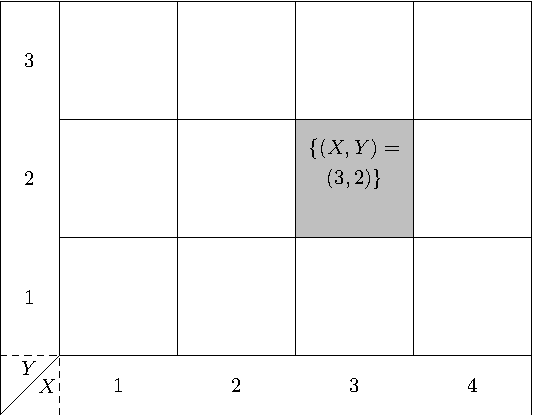
\includegraphics[keepaspectratio]{VA_generali_files/figure-pdf/unnamed-chunk-10-1.pdf}}

}

\caption{Rappresentazione del sistema di alternative associato alla
variabile congiunta \((X,Y)\), in grigio l'evento \((X,Y)=  (3,2)\).}

\end{figure}%

In questa costruzione, le variabili \(X\), \(Y\) (considerate
separatamente) sono dette \emph{marginali} della variabile congiunta
\((X,Y)\). La domanda principale cui cerchiamo di rispondere è la
seguente: come determinare la legge della variabile congiunta?

Cominciamo da un fatto più semplice: dalla legge congiunta è sempre
possibile ottenere le leggi delle marginali, tramite composizione di
opportune funzioni di proiezione. In particolare, la variabile \(X\) è
ottenibile tramite la funzione
\[ g: E\times F \to E, \quad (x,y) \mapsto x.\] Pertanto, se la
variabile congiunta \((X,Y)\) ammette densità discreta, si ottiene che
la densità discreta di \(X\) in \(x \in E\) è data dalla somma su tutti
i possibili valori in \(g^{-1}(x)\), ossia le coppie del tipo \((x,y)\),
al variare di \(y \in F\). Troviamo quindi
\[ P(X = x|I) = \sum_{y \in F} P(X=x, Y=y|I) =\sum_{y \in F} P( (X,Y) =(x, y) |I).\]

Similmente, si trova
\[ P(Y = y | I) = \sum_{x \in E} P( (X,Y) = (x,y) |I).\]

Per trattare il caso di una variabile congiunta \((X,Y)\) con densità
continua, dobbiamo richiedere che \(E = \R^{d}\), \(F = \R^{k}\) in modo
che \(E\times F = \R^{d+k}\). Supponendo che la variabile congiunta
\((X,Y)\) ammetta densità continua \(p((X,Y) = (x,y)|I)\), con
\(x \in \R^d\), \(y\in \R^k\), si può mostrare (usando la definizione
che abbiamo dato) che la densità delle marginali si trova integrando
sulle variabil ``libere'': per la densità di \(X\), si ha
\[ p(X = x | I) = \int_{\R^k} p( (X,Y)= (x,y) |I) d y,\] mentre
\[ p(Y = y | I) = \int_{\R^d} p( (X,Y) = (x,y) |I) d x,\] avendo usato
una notazione compatta per l'integrale in più variabili.

La domanda successiva è quindi se la conoscenza delle leggi delle
variabili \(X\) e \(Y\) (separatamente) sia sufficiente per determinare
la legge della variabile congiunta. Si vede immediatamente che questo è
falso, considerando il seguente esempio di estrazioni dall'urna.

Sia data un'urna contenente al solito \(N\) palline di cui \(R\) rosse e
\(B\) blu (parametri noti). Si consideri una variabile
\(X \in \cur{0,1}\) che indica se nella prima estrazione la pallina
estratta è rossa, e una seconda variabile \(Y \in \cur{0,1}\) che indica
se nella seconda estrazione la pallina è rossa. Sia che le estrazioni
siano con oppure senza rimpiazzo, abbiamo visto nel Capitolo
Capitolo~\ref{sec-intro-prob} che
\[ P(X = 1 | \Omega) = P(Y = 1 | \Omega ) = \frac{R}{N}.\] Tuttavia, se
le estrazioni sono senza rimpiazzo, vale
\[\begin{split} P((X,Y) = (1,1) |\Omega) & = P(X = 1 |\Omega) P(Y = 1 | X=1) \\
& = \frac{R}{N} \cdot \frac{R-1}{N-1},\end{split}\] mentre se sono con
rimpiazzo, per indipendenza vale
\[ \begin{split} P((X,Y) = (1,1) |\Omega) &= P(X = 1 |\Omega) P(Y = 1 | X=1) =P(X = 1 |\Omega) P(Y = 1 | \Omega) \\
& = \frac{R}{N} \cdot \frac{R}{N}.
\end{split}\]

Prima di concludere questa sezione, osserviamo che la costruzione
introdotta si estende al caso di un numero qualsiasi (finito) \(k\)
variabili aleatorie \(X_1\in E_1\), \ldots, \(X_k \in E_k\). La
variabile congiunta \(X = (X_1, \ldots, X_k)\) è a valori nelle
\(k\)-uple ordinate
\[x = (x_1, \ldots, x_k) \in E_1 \times \ldots \times E_k\] ed è
definita tramite il sistema di alternative
\[\begin{split} \cur{ X = x} & = \cur{X_1 = x_1, X_2=x_2, \ldots, X_k = x_k} \\
& = \cur{X_1 = x_1} \text{ e } \ldots  \cur{X_k = x_k}.\end{split}\] Per
ottenere le leggi marginali, o più in generale la legge di una variabile
congiunta \((X_i)_{i \in I}\) per un sottoinsieme di indici
\(I \subseteq \cur{1, \ldots, k}\), è sufficiente sommare (o integrare)
la densità della variabile congiunta rispetto alle variabili ``libere'',
ossia associate agli indici nel complementare di \(I\).

\subsection{Esercizi}\label{esercizi-12}

Dare un esempio di due leggi marginali entrambe su \(E= \cur{1,2,3,4}\)
tali che esistano (almeno) tre leggi congiunte \(E\times E\) diverse con
tali leggi marginali.

Nel modello dell'estrazione dall'urna senza rimpiazzo, considerare
variabili aleatorie \(X_1\), \(X_2\), \ldots, \(X_5\) a valori in
\(E = \cur{R, B}\) rappresentanti l'esito della prima, seconda, ecc.
estrazione. Scrivere esplicitamente la densità discreta congiunta di
\(X=(X_1, X_2, \ldots, X_5)\) e le densità marginali.

\section{Formula di Bayes per variabili aleatorie}\label{sec-bayes-va}

Abbiamo visto che la densità di una variabile congiunta non è
esprimibile in termini delle due densità marginali (rispetto
all'informazione nota \(I\)). Un modo per aggirare questo problema è
fornito dalla regola del prodotto, che garantisce (evitiamo di scrivere
\(I\) per semplicità)
\[ P( (X,Y) = (x,y)) = P(X=x \text{ e } Y = y ) = P(X=x) P(Y=y |  X=x).\]
Possiamo leggere questa identità nel seguente modo: nel caso di
variabili discrete, la densità della variabile congiunta è determinata
da 1. La densità della marginale \(X\) 2. La densità della marginale
\(Y\), ma condizionata all'informazione \(X=x\) per ciascun \(x \in E\)
(che si abbrevia dicendo semplicemente condizionata ad \(X\)).

In pratica in molti casi la legge congiunta è proprio definita tramite
queste due quantità (la densità di una marginale e la densità dell'altra
marginale condizionata alla prima).

Nel caso delle due estrazioni dall'urna la densità congiunta della prima
e della seconda estrazione è definita nell'ordine naturale, partendo
dalla prima estrazione e poi specificando la densità della seconda
condizionata alla prima (e distinguendo quindi tra estrazioni con e
senza rimpiazzo). Ovviamente nulla vieta di considerare anche altre
densità condizionate, ad esempio invece di aggiungere la stessa pallina
si potrebbe sostituire la pallina estratta con una dell'altro colore. In
tal caso, ponendo come nella sezione precedente \(X\) la variabile
indicatrice della prima estrazione (\(1\) se è rossa), \(Y\) invece
relativa alla seconda estrazione, si trova
\[ P(Y =1 | X=1) = \frac{R-1}{N}, \quad  P(Y =1 | X=0) = \frac{R+1}{N},\]
che permette di definire una ulteriore densità congiunta per la
variabile \((X,Y)\) (ovviamente densità congiunte diverse servono a
descrivere situazioni diverse).

La formula di Bayes si può quindi riscrivere in termini di variabili
aleatorie, ottenendo
\[ P(X=x | Y =y ) = P(X=x) \cdot  \frac{ P(Y=y | X=x)}{P(Y=y)} \propto P(X=x)L(X=x; Y=y),\]
con la stessa inteprertazione del caso di sistemi di alternative (è in
effetti solamente un cambio di notazione). Ricordiamo che il rapporto
\[ \frac{ P(Y=y | X=x)}{P(Y=y)} = \frac{ P(X=x | Y=y)}{P(X=x)}\] non
cambia se si scambiano i ruoli di \(X=x\) ed \(Y=y\), e indica quando
l'osservazione di uno dei due eventi aumenti (se maggiore di \(1\)),
diminuisca (se minore di \(1\)) il grado di fiducia nell'altro evento.
Come nel caso delle alternative, in molti casi si è semplicemente
interessati al valore più probabile della \(X\), avendo osservato
\(Y=y\). Si definisce pertanto la stima di massimo a posteriori per la
\(X\), avendo osservato \(y=y\), come il valore (o i valori)
\[ x_{\map} \in \arg \max \cur{ P(X=x) L(X=x; Y=y) : x \in E}\] e
ricordiamo che nel caso di \(X\) con densità uniforme discreta su \(E\)
(rispetto all'informazione iniziale) il problema si riduce alla stima di
massima verosimiglianza
\[ x_{\mle} \in  \arg \max \cur{L(X=x; Y=y) : x \in E}.\] In molte
situazioni in cui \(E\) sia infinito, per estensione dal caso finito si
considera il problema sopra (immaginando una distribuzione a priori
uniforme su \(E\), che rigorosamente non esiste, ma è comunque utile).
Vediamo un esempio

Si consideri la seguente situazione: si informa il robot che un'urna
contiene metà palline rosse e metà palline blu, da cui si effettuano un
certo numero di estrazioni con rimpiazzo. Il robot tuttavia non viene
informato del numero esatto delle estrazioni, ma si comunica al robot
solamente che il numero di palline rosse estratte è \(10\). Possiamo
stimare il numero di estrazione effettuate? intuitivamente, la risposta
dovrebbe essere \(20\), ma vediamo come il robot può ragionare.

Definiamo una variabile aleatoria \(M\) che indica il numero di
estrazioni effettuate. Non sapendo nulla su \(M\) (prima di ricevere
l'informazione che \(10\) rosse sono state estratte), il robot suppone
che sia uniformemente distribuita sui valori
\(\cur{0,1, \ldots, \bar{m}}\), per un parametro \(\bar{m}\) molto
grande (idealmente infinito), \[ P(M=m|\Omega) = \frac {1}{\bar{m}}\]
per \(m \le \bar{m}\). Nel definire la densità del numero di rosse
estratte sapendo \(M = m\), il robot utilizza la densità binomiale di
parametri \((m,1/2)\) (perché sa che metà palline sono rosse e metà
blu). Pertanto, posta \(N_R\) la variabile che indica il numero di
palline rosse estratte, si ha
\[ P(  N_R = k | M=m) = {m\choose k} \bra{ \frac{1}{2}}^k \bra{\frac 1 2 }^{m-k} = {m \choose k} \frac {1}{2^m}.\]
La formula di Bayes permette di ottenere la densità di \(M\) avendo
osservato \(N_R = 10\), per \(m \le \bar{m}\),
\[ P(  M=m| N_R = k) = P(M=m|\Omega)\cdot \frac{P(N_R = 10| M=m)}{P(N_R = 10|\Omega)} = \frac{1}{\bar{m}} {m \choose k} \frac {1}{2^m} \cdot \frac{1}{P(N_R = 10|\Omega)}.\]
Un'espressione per \(P(R_R|\Omega)\) si ottiene imponendo che l'ultimo
termine sia una densità discreta (oppure tramite la formula di
disintegrazione)
\[P(N_R|\Omega) = \sum_{m=0}^{\bar{m}} \frac{1}{\bar{m}} {m \choose k} \frac {1}{2^m}.\]
Ora non vale più la pena di proseguire con i calcoli teorici, piuttosto
è meglio plottare la densità e studiare come dipenda dal parametro
\(\bar{m}\).

\begin{Shaded}
\begin{Highlighting}[]
\CommentTok{\# introduciamo due possibili parametri (si consiglia di ripetere con altri valori)}

\NormalTok{possibili\_bar\_m }\OtherTok{\textless{}{-}} \FunctionTok{c}\NormalTok{(}\DecValTok{25}\NormalTok{, }\DecValTok{50}\NormalTok{)}

\CommentTok{\#Inizializziamo  una matrice che conterrà le densità al variare del parametro bar\_m (utile il barplot).}

\NormalTok{dens\_matrice\_M\_NR\_10 }\OtherTok{\textless{}{-}} \FunctionTok{matrix}\NormalTok{( }\DecValTok{0}\NormalTok{, }\AttributeTok{nrow=}\DecValTok{2}\NormalTok{, }\AttributeTok{ncol=}\DecValTok{50}\NormalTok{)}


\CommentTok{\# dovendo ripetere gli stessi calcoli al variare  di bar\_m, utilizziamo un ciclo for}

\ControlFlowTok{for}\NormalTok{ (iter }\ControlFlowTok{in} \DecValTok{1}\SpecialCharTok{:}\DecValTok{2}\NormalTok{)\{}
\NormalTok{  bar\_m }\OtherTok{\textless{}{-}}\NormalTok{ possibili\_bar\_m[iter]}
\NormalTok{  m }\OtherTok{\textless{}{-}} \DecValTok{0}\SpecialCharTok{:}\NormalTok{bar\_m}

\CommentTok{\# scriviamo la verosimiglianza}

\NormalTok{  likelihood }\OtherTok{\textless{}{-}} \FunctionTok{dbinom}\NormalTok{(}\DecValTok{10}\NormalTok{, m, }\DecValTok{1}\SpecialCharTok{/}\DecValTok{2}\NormalTok{)}

\CommentTok{\# la densità discreta di M avendo osservato N\_R = 10 si ottiene moltiplicando la densità a priori (che è costante uguale a 1/bar\_m,) e normalizzando in modo che sommi ad 1 {-}{-} quindi  non serve neppure moltiplicare per 1/bar\_m, ma lo facciamo per chiarezza}

\NormalTok{  dens\_M\_NR\_10 }\OtherTok{\textless{}{-}}\NormalTok{ likelihood}\SpecialCharTok{/}\NormalTok{bar\_m}
\NormalTok{  dens\_M\_NR\_10 }\OtherTok{\textless{}{-}}\NormalTok{ dens\_M\_NR\_10}\SpecialCharTok{/}\FunctionTok{sum}\NormalTok{(dens\_M\_NR\_10)}
\NormalTok{  dens\_matrice\_M\_NR\_10[iter,] }\OtherTok{\textless{}{-}}\NormalTok{ dens\_M\_NR\_10[}\DecValTok{1}\SpecialCharTok{:}\DecValTok{50}\NormalTok{]}
\NormalTok{\}}

\NormalTok{colori }\OtherTok{\textless{}{-}}\NormalTok{ miei\_colori[}\DecValTok{1}\SpecialCharTok{:}\DecValTok{2}\NormalTok{]}

\FunctionTok{barplot}\NormalTok{(dens\_matrice\_M\_NR\_10, }\AttributeTok{beside=}\ConstantTok{TRUE}\NormalTok{, }\AttributeTok{col=}\NormalTok{colori, }\AttributeTok{names.arg =} \FunctionTok{as.character}\NormalTok{(}\DecValTok{0}\SpecialCharTok{:}\DecValTok{49}\NormalTok{), }\AttributeTok{xlab=}\StringTok{\textquotesingle{}numero estrazioni\textquotesingle{}}\NormalTok{, }\AttributeTok{ylab=}\StringTok{\textquotesingle{}densità discreta\textquotesingle{}}\NormalTok{)}


\CommentTok{\# aggiungiamo una legenda}

\FunctionTok{legend}\NormalTok{(}\StringTok{\textquotesingle{}topright\textquotesingle{}}\NormalTok{, }\AttributeTok{legend=}\FunctionTok{c}\NormalTok{(}\StringTok{\textquotesingle{}bar\_m = 25\textquotesingle{}}\NormalTok{, }\StringTok{\textquotesingle{}bar\_m = 50\textquotesingle{}}\NormalTok{), }\AttributeTok{fill=}\NormalTok{colori)}
\end{Highlighting}
\end{Shaded}

\begin{figure}[H]

{\centering \pandocbounded{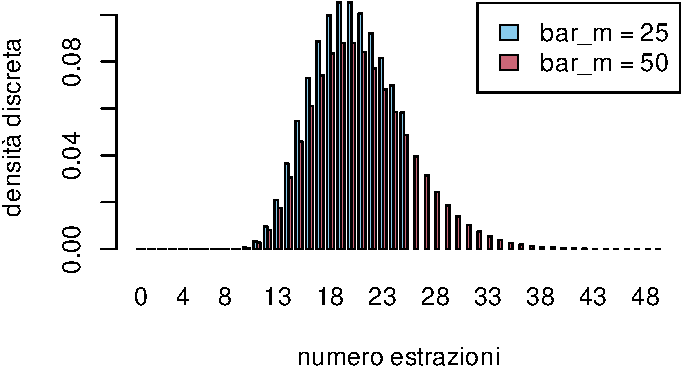
\includegraphics[keepaspectratio]{VA_generali_files/figure-pdf/unnamed-chunk-11-1.pdf}}

}

\caption{grafico della densità discreta di \(M\) sapendo \(N_R=10\), al
variare del parametro \(\bar{m}\)}

\end{figure}%

Osserviamo che se \(\bar{m}\) è piccolo, la densità di \(M\) varia
abbastanza, tuttavia al crescere di \(\bar{m}\) si stabilizza in un
opportuno profilo. Pertanto il risultato non dipende essenzialmente da
\(\bar{m}\) (che si può anche mandare all'infinito, per essere formali).

Inoltre, la stima di massima verosimiglianza \(m_{\mle}\) si può
ottenere dai calcoli svolti sopra.

\begin{Shaded}
\begin{Highlighting}[]
\CommentTok{\# la funzione which.max restituisce l\textquotesingle{}indice corrispondente al punto di massimo di un vettore}

\NormalTok{indice\_max }\OtherTok{=} \FunctionTok{which.max}\NormalTok{(dens\_M\_NR\_10)}

\CommentTok{\# di conseguenza m\_max si ottiene dalla componente di indice\_max del vettore m}

\NormalTok{(}\AttributeTok{m\_max =}\NormalTok{ m[indice\_max])}
\end{Highlighting}
\end{Shaded}

\begin{verbatim}
[1] 19
\end{verbatim}

\begin{Shaded}
\begin{Highlighting}[]
\CommentTok{\# la risposta potrebbe stupirci, ma confrontiamo le probabilità a posteriori}

\NormalTok{dens\_M\_NR\_10[indice\_max] }\CommentTok{\# per la probabilità che M=19}
\end{Highlighting}
\end{Shaded}

\begin{verbatim}
[1] 0.08809918
\end{verbatim}

\begin{Shaded}
\begin{Highlighting}[]
\NormalTok{dens\_M\_NR\_10[indice\_max}\SpecialCharTok{+}\DecValTok{1}\NormalTok{] }\CommentTok{\# per la probabilità che M=20}
\end{Highlighting}
\end{Shaded}

\begin{verbatim}
[1] 0.08809918
\end{verbatim}

Questa costruzione, che è essenzialmente la regola del prodotto e la
conseguente formula di Bayes, si estende in diversi modi. Il primo è di
considerare variabili continue. In tal caso, per definire la densità
continua della congiunta, si deve mostrare una versione della regola del
prodotto per le densità, precisamente, per \(X \in \R^d\),
\(Y \in \R^k\),
\[ p((X,Y)=(x,y) ) = p(X=x, Y=y) = p(X=x) p(Y=y | X=x),\] dove il
termine \(p(Y=y|X=x)\) è detto anche \emph{densità condizionale} di
\(Y\) rispetto ad \(X\) ed è la densità della variabile \(Y\) sapendo,
oltre all'informazione \(I\) qui non scritta, anche che \(X\) assume il
valore \(x\). Il modo più semplice per pensare a questa formula è che
sia una definizione della densità della congiunta partendo dalla densità
continua di \(X\) e dalla densità di \(Y\) sapendo \(X=x\). Si può anche
leggere al contrario, ossia conoscendo la densità della variabile
congiunta, si ricava una versione della fomula di Kolmogorov per densità
continue \[  p(Y =y | X=x) = \frac{ p(X=x, Y=y)}{p(X=x)}.\]

La costruzione è perfettamente simmetrica, e invertendone l'ordine si
ottiene la formula di Bayes per densità continue:
\[ p(X=x | Y =y ) = p(X=x) \cdot  \frac{ p(Y=y | X=x)}{p(Y=y)} \propto p(X=x) L(X=x; Y=y),\]
con la stessa intepretazione che nel caso discreto (eccetto che stiamo
trattando densità continue e non probabilità). Per determinare il
denominatore, possiamo sempre ricordare che l'integrale della densità a
sinistra (come funzione di \(x\)) deve valere \(1\), da cui si trova una
formula di disintegrazione per densità continue:
\[ p(Y=y) = \int_{\R^d}   p(Y=y | X=x) p(X=x)d x = \int_{\R^d} L(X=x; Y=y) p(X=x) dx.\]
Analogamente a quanto accadeva nel caso discreto, il rapporto
\[  \frac{ p(Y=y | X=x)}{p(Y=y)}  = \frac{ p(X=x | Y=y)}{p(X=x)} \] non
cambia se si scambiano gli eventi \(Y=y\), \(X=x\). Come nel caso
discreto, per determinare l'alternativa \(\cur{X=x}\) più probabile,
avendo osservato \(\cur{Y=y}\), è sufficiente trovare il (o i) punti di
massimo della funzione \[ x \mapsto  p(X=x) L(X=x; Y=y),\] determinando
così la stima del massimo a posteriori per \(X\) avendo osservato
\(Y=y\).

\begin{remark}[massima verosimiglianza nel caso continuo]
Nel caso in cui \(X\) sia una variabile uniforme (ad esempio, su un
intervallo \([a,b]\)), come nel caso discreto il problema di determinare
i punti di massimo per la distribuzione condizionata all'osservazione di
\(Y\), si riduce a
\[ x_{\mle} \in \operatorname{arg}\cur{ \max p(Y=y | X=x): x \in [a,b]}.\]
Tale \(x_{\mle}\) è il caso continuo della stima di massima
verosimiglianza della variabile \(X\), avendo osservato \(Y=y\). Spesso,
si massimizza direttamente al variare di \(x \in \R\) o su un intervallo
illimitato, come una semiretta (anche se propriamente non esiste una
densità continua uniforme su intervalli illimitati).
\end{remark}

Vediamo un esempio di applicazione della formula di Bayes e della stima
massima verosimiglianza nel caso continuo. Si vuole modellizare la
durata della carica di un dispositivo (ad esempio, uno smartphone, o un
drone) tramite una variabile aleatoria \(T\) avente densità continua
esponenziale di un certo parametro \(\lambda\). Questo semplice modello
contiene il solo parametro \(\lambda\), appunto, che inizialmente
possiamo supporre uniformemente distribuito nei valori \([0,1]\) (ad
esempio, misurando in giorni, e ricordando che tanto più piccolo è
\(\lambda\), maggiori sono i valori assunti da \(T\)). Il robot
considera quindi una variabile \(\Lambda\) uniforme continua su
\([0,1]\) (rispetto alla informazione iniziale \(\Omega\)). Condizionata
a \(\Lambda= \lambda\), \(T\) ha una densità esponenziale di parametro
\(\lambda\),
\[p(T = t | \Lambda = \lambda) = \lambda e^{-\lambda t } \quad \text{per $t \ge 0$.}\]
Avendo osservato che (per un dispositivo) la sua durata è \(T=10\),
possiamo ottenere la densità di \(\Lambda\) aggiornata a questa
informazione: per \(\lambda \in [0,1]\),
\[ p(\Lambda = \lambda| T = 10) = p(\Lambda = \lambda|\Omega) p(T=10 | \Lambda = \lambda) \cdot \frac{1}{p(T=10|\Omega)} = p(T=10 | \Lambda = \lambda) \cdot \frac{1}{p(T=10|\Omega)},\]
ricordando l'ipotesi che \(\Lambda\) sia uniforme (rispetto a
\(\Omega\)). Per determinare il denominatore esplicitamente, basta
imporre che il membro a destra sia una densità continua (rispetto a
\(\lambda\)) e quindi integrare ad \(1\). Si trova la formula
\[ p(T=10|\Omega) = \int_0^1  \lambda e^{- 10 \lambda } d \lambda.\] Non
vale la pena di cercare una espressione in termini di funzioni
elementari, ma è più utile tracciarne un grafico approssimato.

\begin{Shaded}
\begin{Highlighting}[]
\NormalTok{delta\_lambda }\OtherTok{\textless{}{-}} \FloatTok{0.01}
\NormalTok{lambda }\OtherTok{\textless{}{-}} \FunctionTok{seq}\NormalTok{(}\DecValTok{0}\NormalTok{, }\DecValTok{1}\NormalTok{, }\AttributeTok{by=}\NormalTok{delta\_lambda)}

\CommentTok{\# scriviamo la verosimiglianza, ossia P(T=10|Lambda=lambda)}

\NormalTok{likelihood }\OtherTok{\textless{}{-}}\NormalTok{ lambda}\SpecialCharTok{*}\FunctionTok{exp}\NormalTok{(}\SpecialCharTok{{-}}\NormalTok{lambda}\SpecialCharTok{*}\DecValTok{10}\NormalTok{)}

\CommentTok{\# otteniamo la distribuzione di Lambda moltiplicando la densità a priori (che vale 1 in questo caso) per la verosimiglianza e normalizzando dividendo per l\textquotesingle{}integrale approssimato tramite somme di Riemann}

\NormalTok{dens\_Lambda\_T\_10 }\OtherTok{\textless{}{-}}\NormalTok{ likelihood}
\NormalTok{dens\_Lambda\_T\_10 }\OtherTok{\textless{}{-}}\NormalTok{ dens\_Lambda\_T\_10}\SpecialCharTok{/}\NormalTok{(}\FunctionTok{sum}\NormalTok{(dens\_Lambda\_T\_10)}\SpecialCharTok{*}\NormalTok{delta\_lambda)}

\CommentTok{\# plottiamo sia la distribuzione a priori (uniforme) che quella condizionata}

\FunctionTok{plot}\NormalTok{(}\ConstantTok{NULL}\NormalTok{, }\AttributeTok{xlim=}\FunctionTok{c}\NormalTok{(}\DecValTok{0}\NormalTok{,}\DecValTok{1}\NormalTok{), }\AttributeTok{ylim=}\FunctionTok{c}\NormalTok{(}\DecValTok{0}\NormalTok{,}\DecValTok{4}\NormalTok{), }\AttributeTok{xlab=}\StringTok{\textquotesingle{}lambda\textquotesingle{}}\NormalTok{, }\AttributeTok{ylab=}\StringTok{\textquotesingle{}densità\textquotesingle{}}\NormalTok{)}

\FunctionTok{lines}\NormalTok{(lambda, }\FunctionTok{dunif}\NormalTok{(lambda), }\AttributeTok{type=}\StringTok{\textquotesingle{}l\textquotesingle{}}\NormalTok{, }\AttributeTok{lwd=}\DecValTok{3}\NormalTok{, }\AttributeTok{col=}\NormalTok{miei\_colori[}\DecValTok{1}\NormalTok{])}

\FunctionTok{lines}\NormalTok{(lambda, dens\_Lambda\_T\_10, }\AttributeTok{type=}\StringTok{\textquotesingle{}l\textquotesingle{}}\NormalTok{, }\AttributeTok{lwd=}\DecValTok{3}\NormalTok{, }\AttributeTok{col=}\NormalTok{miei\_colori[}\DecValTok{2}\NormalTok{])}



\CommentTok{\# aggiungiamo una legenda}

\FunctionTok{legend}\NormalTok{(}\StringTok{\textquotesingle{}topright\textquotesingle{}}\NormalTok{, }\AttributeTok{legend=}\FunctionTok{c}\NormalTok{(}\StringTok{\textquotesingle{}a priori\textquotesingle{}}\NormalTok{, }\StringTok{\textquotesingle{}condizionata a T=10\textquotesingle{}}\NormalTok{), }\AttributeTok{fill=}\NormalTok{miei\_colori[}\DecValTok{1}\SpecialCharTok{:}\DecValTok{2}\NormalTok{])}
\end{Highlighting}
\end{Shaded}

\begin{figure}[H]

{\centering \pandocbounded{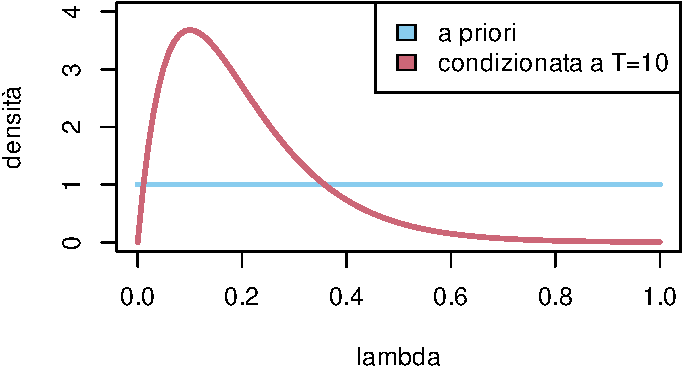
\includegraphics[keepaspectratio]{VA_generali_files/figure-pdf/unnamed-chunk-13-1.pdf}}

}

\caption{densità per \(\Lambda\): a priori e avendo osservato \(T=10\)}

\end{figure}%

Se si è interessati alla stima di massima verosimiglianza, si
determinare
\[ \lambda_{\mle} \in \arg \max \cur{ \lambda e^{- 10 \lambda } : \lambda \in [0,1]},\]
e in questo caso il problema ha una semplice soluzione analitica. Basta
derivare e imporre che la derivata sia nulla, trovando
\[   e^{- 10 \lambda } - 10 \lambda e^{-10 \lambda} = 0 \quad \text{ossia} \quad  \lambda = 1/10.\]
(andrebbe anche verificato che il massimo non sia raggiunto agli estremi
dell'intervallo, ma dal grafico sopra è evidente). Per modelli più
complicati, si deve ricorrere a metodi numerici per determinare la stima
di massima verosimiglianza. Possiamo anche accontentarci del risultato
approssimato ottenuto dai valori plottati sopra.

\begin{Shaded}
\begin{Highlighting}[]
\NormalTok{indice\_max }\OtherTok{\textless{}{-}} \FunctionTok{which.max}\NormalTok{(dens\_Lambda\_T\_10)}

\CommentTok{\# per ottenere la stima di massima verosimiglianza basta ottere la componente dal vettore lambda}

\NormalTok{lambda[indice\_max]}
\end{Highlighting}
\end{Shaded}

\begin{verbatim}
[1] 0.1
\end{verbatim}

consideri una variabile aleatoria \(\Lambda\) a valori in \([0, 10]\)
uniforme (rispetto ad una informazione iniziale \(\Omega\))

Vale la pena di menzionare anche il caso misto, in cui \(X \in E\) ha
densità discreta mentre \(Y\), condizionata ad \(\cur{X=x}\), è
continua, per ogni \(x \in E\). In tal caso il problema è che in
generale la variabile congiunta non ha densità né continua né discreta,
tuttavia la formula di Bayes rimane valida, nella forma
\[ P(X = x | Y=y ) = P(X =x)\cdot \frac{ p(Y= y| X=x)}{p(Y=y)} \propto P(X=x) L(X=x; Y=y)\]
e al solito imponendo che sia una densità discreta e quindi sommi ad
\(1\) si trova per il denominatore l'espressione
\[ p(Y=y) = \sum_{x \in E}  p(Y= y| X=x)P(X =x).\] Vale anche la formula
nel caso simmetrico (ossia \(X\in \R^d\) è continua mentre \(Y\),
condizionata ad \(\cur{X=x}\) è discreta):
\[ p(X=x | Y=y) = p(X=x) \cdot \frac{ P(Y= y| X=x)}{P(Y=y)} \propto p(X=x) L(X=x; Y=y)\]
con \[ P(Y=y) = \int_{\R^d}  P(Y= y| X=x)p(X =x) dx.\] Anche in questo
caso è utile studiare la stima di massimo a posteriori o di massima
verosimiglianza per \(X\) avendo osservato \(Y=y\) (non ripetiamo la
definizione, che è praticamente la stessa, con le dovute modifiche).

\protect\phantomsection\label{bayes-continuo}
Per fare un esempio di questo caso ``misto'', si supponga che il robot
sia stato informato che un'urna contiene palline rosse oppure blu, ma
non del numero totale né della frazione di palline rosse sul totale.
Successivamente viene informato che, avendo effettuato \(10\) estrazioni
con rimpiazzo, sono state osservate \(3\) palline rosse. Come stimare la
frazione di palline rosse sul totale? Intuitivamente capiamo che la
risposta è \(3/10\), ma vediamo come ragiona il robot.

Il robot introduce una variabile aleatoria \(F_R \in [0,1]\) per
indicare la frazione di palline rosse. Rispetto alla informazione
iniziale (prima di sapere delle \(10\) estrazioni), suppone che abbia
densità uniforme continua. Introduce poi la variabile \(N_R\) che indica
il numero di palline rosse estratte nelle \(10\) estrazioni. Sapendo
\(F_R = r\), \(N_R\) ha densità discreta Binomiale di parametri
\(n =10\) (numero di estrazioni) e \(p = r\) (probabilità di estrarre
una rossa). Pertanto, per \(k \in \cur{0, \ldots, 10}\),
\[ P(N_R = k | F_R = r) = { 10 \choose k} r^k (1-r)^{10-k}.\] Avendo
osservato \(N_R =3\), la formula di Bayes (nel caso ``misto'' discreto e
continuo) diventa, per \(r \in [0,1]\),
\[ p( F_R = r | N_R = 3) = p(F_R = r|\Omega) \frac{ P(N_R=3 | F_R = r)}{P(N_R = 3|\Omega)} = { 10 \choose 3} r^3 (1-r)^{7} \cdot \frac{1}{P(N_R = 3 | \Omega)},\]
icordando che \(p(F_R = r| \Omega) = 1\) (la densità a priori è
uniforme). Troviamo anche una espressione per il denominatore -- anche
se abbiamo capito che per molti aspetti non serve -- imponendo che il
membro a destra sia una densità continua
\[ P(N_R = 3 | \Omega) = \int_0^1 { 10 \choose 3} r^3 (1-r)^{7} d r.\]
Si tratta di integrare un polinomio, quindi con un po' di lavoro (oppure
l'uso di un integratore simbolico) si può anche ottenere una formula
esplicita. Tuttavia possiamo anche limitarci allo studio numerico.

\begin{Shaded}
\begin{Highlighting}[]
\NormalTok{delta\_fr }\OtherTok{\textless{}{-}} \FloatTok{0.01}
\NormalTok{fr }\OtherTok{\textless{}{-}} \FunctionTok{seq}\NormalTok{(}\DecValTok{0}\NormalTok{, }\DecValTok{1}\NormalTok{, }\AttributeTok{by=}\NormalTok{delta\_fr)}

\CommentTok{\# scriviamo la verosimiglianza}

\NormalTok{likelihood }\OtherTok{\textless{}{-}} \FunctionTok{dbinom}\NormalTok{(}\DecValTok{3}\NormalTok{, }\DecValTok{10}\NormalTok{, fr)}

\CommentTok{\# otteniamo la distribuzione di F\_R moltiplicando la densità a priori (che vale 1 in questo caso) per la verosimiglianza e normalizzando dividendo per l\textquotesingle{}integrale approssimato tramite somme di Riemann}

\NormalTok{dens\_FR\_NR\_3 }\OtherTok{\textless{}{-}}\NormalTok{ likelihood}
\NormalTok{dens\_FR\_NR\_3 }\OtherTok{\textless{}{-}}\NormalTok{ dens\_FR\_NR\_3}\SpecialCharTok{/}\NormalTok{(}\FunctionTok{sum}\NormalTok{(dens\_FR\_NR\_3)}\SpecialCharTok{*}\NormalTok{delta\_fr)}

\CommentTok{\# plottiamo sia la distribuzione a priori (uniforme) che quella condizionata}

\FunctionTok{plot}\NormalTok{(}\ConstantTok{NULL}\NormalTok{, }\AttributeTok{xlim=}\FunctionTok{c}\NormalTok{(}\DecValTok{0}\NormalTok{,}\DecValTok{1}\NormalTok{), }\AttributeTok{ylim=}\FunctionTok{c}\NormalTok{(}\DecValTok{0}\NormalTok{,}\DecValTok{3}\NormalTok{), }\AttributeTok{xlab=}\StringTok{\textquotesingle{}frazione di palline rosse\textquotesingle{}}\NormalTok{, }\AttributeTok{ylab=}\StringTok{\textquotesingle{}densità\textquotesingle{}}\NormalTok{)}

\FunctionTok{lines}\NormalTok{(fr, }\FunctionTok{dunif}\NormalTok{(fr), }\AttributeTok{type=}\StringTok{\textquotesingle{}l\textquotesingle{}}\NormalTok{, }\AttributeTok{col=}\NormalTok{miei\_colori[}\DecValTok{1}\NormalTok{], }\AttributeTok{lwd=}\DecValTok{3}\NormalTok{)}


\FunctionTok{lines}\NormalTok{(fr, dens\_FR\_NR\_3, }\AttributeTok{type=}\StringTok{\textquotesingle{}l\textquotesingle{}}\NormalTok{, }\AttributeTok{col=}\NormalTok{miei\_colori[}\DecValTok{2}\NormalTok{], }\AttributeTok{lwd=}\DecValTok{3}\NormalTok{)}


\CommentTok{\# aggiungiamo una legenda}

\FunctionTok{legend}\NormalTok{(}\StringTok{\textquotesingle{}topright\textquotesingle{}}\NormalTok{, }\AttributeTok{legend=}\FunctionTok{c}\NormalTok{(}\StringTok{\textquotesingle{}a priori\textquotesingle{}}\NormalTok{, }\StringTok{\textquotesingle{}condizionata a N\_R=10\textquotesingle{}}\NormalTok{), }\AttributeTok{fill=}\NormalTok{miei\_colori[}\DecValTok{1}\SpecialCharTok{:}\DecValTok{2}\NormalTok{])}
\end{Highlighting}
\end{Shaded}

\begin{figure}[H]

{\centering \pandocbounded{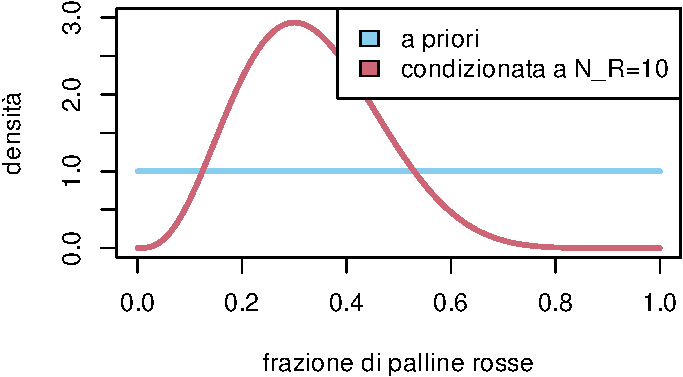
\includegraphics[keepaspectratio]{VA_generali_files/figure-pdf/unnamed-chunk-15-1.pdf}}

}

\caption{densità continua della frazione di palline rosse a priori e
avendo osservato in \(10\) estrazioni con rimpiazzo \(3\) palline rosse}

\end{figure}%

Osserviamo in particolare come la densità si sia accumulata intorno al
punto di massima verosimiglianza, che possiamo calcolare numericamente
al solito modo:

\begin{Shaded}
\begin{Highlighting}[]
\NormalTok{fr[}\FunctionTok{which.max}\NormalTok{(dens\_FR\_NR\_3)]}
\end{Highlighting}
\end{Shaded}

\begin{verbatim}
[1] 0.3
\end{verbatim}

che conferma la nostra intuizione. Osserviamo anche che la densità vale
\(0\) nei casi estremi \(F_R=0\) oppure \(F_R = 1\): questo riflette il
fatto che il robot abbia osservato almeno una pallina rossa e almeno una
blu dentro l'urna.

\subsection{Esercizi}\label{esercizi-13}

Ripetere gli esempi con densità non uniformi (ad esempio partendo dalle
densità a posteriori ottenute)

\section{Indipendenza}\label{sec-indipendenza-va}

In questa sezione estendiamo il concetto di indipendenza tra sistemi di
alternative riformulandolo in termini di variabili aleatorie e delle
loro densità (discrete e continue).

La Definizione \textbf{?@def-indipendenza} si traduce immediatamente da
sistemi di alternative finiti a variabili aleatorie discrete, nel
seguente modo.

Siano \(X_1\in E_1\), \ldots \(X_k\in E_k\) variabili aleatorie con
densità discreta (rispetto ad una informazione nota \(I\)). Allora esse
si dicono indipendenti (condizionatamente ad \(I\)) se vale
\[ P( X_1 =x_1, X_2 = x_2, \ldots, X_k=x_k|I) = \prod_{i=1}^k P(X_i = x_i|I),\]
per ogni \(x_1 \in E_1\), \(x_2 \in E_2\), \ldots, \(x_k \in E_k\), o
equivalentemente, per ogni sottoinsieme
\(J \subseteq \cur{1, \ldots, k}\),
\[ P( X_j =x_j \text{ per ogni $j \in J$} |I,X_\ell = x_\ell \text{ per ogni $\ell \notin J$}  ) =  P(X_j = x_j \text{ per ogni $j \in J$} |I ). \]

Notiamo che il membro a sinistra è la densità discreta della variabile
congiunta \((X_1, \ldots, X_k)\), mentre a destra abbiamo il prodotto
delle densità discrete delle marginali. Questo suggerisce come definire
l'indipendenza probabilistica tra \(k\) variabili aventi densità
continua, nel seguente modo.

Siano \(X_1\in \R^{d_1}\), \ldots \(X_k\in \R^{d_k}\) variabili
aleatorie con densità continua (rispetto ad una informazione nota
\(I\)). Allora esse si dicono indipendenti (condizionatamente ad \(I\))
se la variabile congiunta \(X = (X_1, \ldots, X_k)\) ammette densità
continua e vale
\[ p(X = x| I ) = p( X_1 =x_1, X_2 = x_2, \ldots, X_k=x_k|I) = \prod_{i=1}^k p(X_i = x_i|I),\]
per ogni \(x_1 \in \R^{d_1}\), \(x_2 \in \R^{d_2}\), \ldots,
\(x_k \in \R^{d_k}\), o equivalentemente, per ogni sottoinsieme
\(J \subseteq \cur{1, \ldots, k}\),
\[ p( X_j =x_j \text{ per ogni $j \in J$} |I,X_\ell = x_\ell \text{ per ogni $\ell \notin J$}  ) =  p(X_j = x_j \text{ per ogni $j \in J$} |I ). \]

Possiamo immaginare definizioni valide anche per i casi ``misti'', in
cui alcune variabili sono discrete e altre continue. Tuttavia non è
necessario, in quanto è possibile dare una definizione generale di
variabili aleatorie indipendenti, che si dimostra equivalente a quelle
date sopra nei casi speciali, ma copre anche altri casi. Il vantaggio
delle definizioni sopra è che sono facili da verificare e coprono casi
molto frequenti.

Siano \(X_1\in E_1\), \ldots \(X_k\in E_k\) variabili aleatorie
(generali). Allora esse si dicono indipendenti (condizionatamente ad una
informazione nota \(I\)) se vale
\[  P( X_1 \in U_1, X_2 \in U_2, \ldots, X_k \in U_k |I) = \prod_{i=1}^k P(X_i \in U_i |I),\]
per ogni \(U_1 \subseteq E_1\), \(U_2 \subseteq E_2\), \ldots{}
\(U_k \subseteq E_k\), o equivalentemente, per ogni sottoinsieme
\(J \subseteq \cur{1, \ldots, k}\),
\[ P( X_j \in U_j \text{ per ogni $j \in J$} |I,X_\ell\in U_\ell \text{ per ogni $\ell \notin J$}  ) =  P(X_j \in U_j \text{ per ogni $j \in J$} |I ). \]

Ricordiamo che, per due affermazioni \(A\), \(B\), l'indipendenza
probabilisticà (condizionatamente ad \(I\)) si esprime equivalentemente
richiedendo che
\[ \frac{ P(A| I, B)}{P(A|I)} = \frac{P(B|I,A)}{P(B|I)} =1,\] che si
interpreta nel seguente modo: aggiungere l'informazione \(B\) ad \(I\)
non cambia il grado di fiducia in \(A\) (e viceversa). Per ottenere una
caratterizzazione simile nel caso di variabili aleatorie, ossia ridurci
a coppie di affermazioni, dobbiamo introdurre il concetto di
``informazione'' associata ad una famiglia di variabili aleatorie
\(\cur{Y_1, \ldots, Y_m}\), definita come una qualsiasi affermazione
riguardante tali variabili (e solo quelle). Formalmente, si può
considerare la variabile congiunta \(Y = (Y_1, \ldots, Y_m)\) e dire che
una informazione \(A\) associata alle variabili
\(\cur{Y_1, \ldots, Y_m}\) è una qualsiasi affermazione del tipo
\[\cur{Y \in U}, \quad \text{dove $U$ è un sottoinsieme dei possibili valori di $Y$.}\]

Con questa notazione possiamo caratterizzare ulteriormente
l'indipendenza probabilistica tra \(k\) variabili aleatorie (non diamo
la dimostrazione di questo risultato, piuttosto tecnico).

Siano \(X_1\in E_1\), \ldots \(X_k\in E_k\) variabili aleatorie
(generali). Allora esse sono indipendenti (condizionatamente ad una
informazione nota \(I\)) se e solo se, dato un qualsiasi sottoinsieme
\(J \subseteq \cur{1, \ldots, k}\), qualsiasi affermazione \(A\)
associata alle variabili \(\cur{X_j}_{j \in J}\) è indipendente (sapendo
\(I\)) da qualsiasi affermazione \(B\) associata alle rimanenti
variabili \(\cur{X_\ell}_{\ell \in \cur{1, \ldots, k}\setminus J}\).

Una conseguenza importante è la seguente.

Date \(X_1\in E_1\), \ldots \(X_k\in E_k\) variabili aleatorie
indipendenti e \(J \subseteq \cur{1, \ldots, k}\), ogni variabile
ottenuta tramite funzione delle \((X_j)_{j \in J}\), è indipendente da
ogni variabile ottenuta tramite funzione delle
\((X_\ell)_{\ell \notin J}\).

La dimostrazione è immediata, poiché ogni informazione associata ad una
variabile composta delle \((X_j)_{j \in J}\) è in particolare associata
alle \(\cur{X_j}_{j \in J}\) (e lo stesso per le rimanenti variabili).

Abbiamo evidenziato l'informazione nota \(I\) in tutte le formule sopra
per ricordare che l'indipendenza tra variabili aleatorie è strettamente
legata all'informazione di cui si dispone. Spesso tale informazione è
del tipo \(\cur{Y=y}\), per una qualche variabile aleatoria \(Y\), e le
variabili \((X_i)_{i=1}^k\) risultato indipendenti per \emph{qualsiasi}
valore \(y\) tra quelle che \(Y\) può assumere. In questo caso, si dice
che le variabili \((X_i)_{i=1}^k\) sono indipendenti condizionatamente
ad \(Y\) (ed eventualmente ulteriore informazione \(I\)).

\subsection{Esercizi}\label{esercizi-14}

Siano \(X\), \(Y\) variabili aleatorie indipendenti a valori interi
\(\mathbb{Z}\). Posta \(Z = X+Y\), mostrare che vale la formula di
convoluzione per la densità discreta,
\[ P( Z = z ) = \sum_{x} P(X=x)P(Y = z-x).\] Calcolare (eventualmente
aiutandosi con R) la densità discreta della somma di due variabili
indipendenti uniformi su \(\cur{1,2,\ldots, 10}\).

\section{Reti bayesiane}\label{sec-bayes-nets}

Finora abbiamo apprezzato come le variabili aleatorie permettano di
gestire sistemi di alternative, anche infiniti, con una notazione
compatta e naturale, anche quando si effettuano operazioni tra di esse.
Tuttavia, confrontando con l'approccio di calcolo delle probabilità
tramite eventi e sistemi di alternative, sarebbe utile disporre di una
rappresentazione grafica, simile a quella dei diagrammi ad albero.
Ovviamente, nel caso di variabili aleatorie con pochi valori è comunque
possibile usare i diagrammi ad albero introducendo le alternative
associate a ciascuna variabile.

Il problema sorge quando si vogliono studiare variabili che assumono
infiniti valori e averne una rappresentazione grafica utile per
scriverne le densità (in generale, ossia congiunte, marginali e
condizionate). Una soluzione è fornita dai diagrammi noti come
\emph{reti Bayesiane}, che definiamo in questa sezione.

Dovendo rappresentare un diagramma associato a \(k\) variabili, \(X\),
\(Y\), \(Z\) ecc., prima di tutto si fissa un ordine tra le variabili
(spesso suggerito dalla struttura del problema che si sta esaminando),
che corrisponde grosso modo all'ordine in cui i sistemi di alternative
vengono aggiunti nella costruzione del grafo ad albero. Per facilitare
la notazione, indichiamo con \(X_1\), \(X_2\), \ldots{} \(X_k\) le
variabili così ordinate. Il diagramma, che è un grafo orientato su \(k\)
nodi corrispondenti alle \(k\) variabili, viene costruito in \(k\)
passi: nel primo passo si introduce solamente il nodo corrispondente
alla variabile \(X_1\); nel passo \(i\)-esimo, si introduce il nodo
corrispondente alla variabile \(X_i\), e si considera la densità di
\(X_i\) (ragioniamo nel caso discreto, per semplicità) condizionata a
tutte le variabili già inserite (quindi \(X_1\), \ldots{} \(X_{i-1}\)),
\[ P(X_i = x_i | I, X_{i-1}=x_{i-1}, \ldots,  X_{1}=x_{1}).\] Si
individua un sottoinsieme (più piccolo possibile)
\(J \subseteq \cur{1, \ldots, i-1}\) tale che la densità sopra dipenda
solo dalle variabili \((X_{j})_{j \in J}\), ossia, per ogni
\(x_1, \ldots, x_i\), valga
\[ P(X_i = x_i | I, X_{i-1}=x_{i-1}, \ldots,  X_{1}=x_{1}) = P(X_i =x_i| I, X_j =x_j \text{ per ogni $j \in J$}).\]
A questo punto si inseriscono gli archi orientati (frecce) da ciascun
nodo corrispondente alle variabili \(X_j\), \(j \in J\), verso il nodo
corrispondente ad \(X_i\). Si ripete la procedura con il passo
successivo (fino a \(i=n\)).

Si considerino \(k\) variabili aleatorie indipendenti \(X_1\), \ldots{}
\(X_k\). L'algoritmo produce il diagramma in figura

\begin{figure}[H]

{\centering \pandocbounded{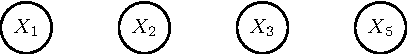
\includegraphics[keepaspectratio]{VA_generali_files/figure-pdf/unnamed-chunk-17-1.pdf}}

}

\caption{Rete bayesiana per \(4\) variabili indipendenti}

\end{figure}%

\protect\phantomsection\label{rete_bayes_lambda_T}
Si consideri una variabile aleatoria \(\Lambda\) tale che,
condizionatamente ad essa, le variabili \(T_1\), \ldots, \(T_k\) sono
indipendenti (un esempio concreto è \(\Lambda= \lambda\) individua il
parametro delle variabili \(T_i\) che hanno legge esponenziale). La
densità congiunta ha la forma
\[ P(\Lambda, T_1, T_2, T_3, T_4) = P(\Lambda) P(T_1|\Lambda) P(T_2|\Lambda) P(T_3|\Lambda)P(T_4|\Lambda).\]
La rete bayesiana costruita inserendo prima la variabile \(\Lambda\) e
poi le rimanenti è rappresentata in figura.

\begin{figure}[H]

{\centering \pandocbounded{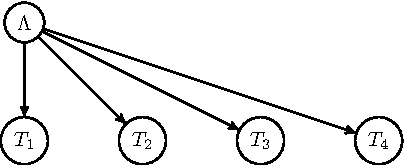
\includegraphics[keepaspectratio]{VA_generali_files/figure-pdf/unnamed-chunk-18-1.pdf}}

}

\caption{Rete bayesiana per \(4\) variabili \(T_1\), \(T_2\), \(T_3\),
\(T_4\) condizionatamente indipendenti rispetto alla variabile
\(\Lambda\)}

\end{figure}%

Si considerino \(k\) variabili \(X_1\), \ldots, \(X_k\) indipendenti tra
loro (rispetto all'informazione iniziale) e sia
\(Y = g(X_1, \ldots, X_k)\) (ad esempio \(Y = X_1+\ldots+X_k\) nel caso
di variabili a valori in \(\R\)). La rete bayesiana è rappresentata in
figura.

\begin{figure}[H]

{\centering \pandocbounded{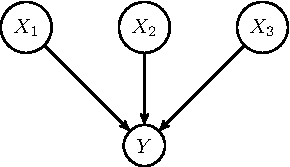
\includegraphics[keepaspectratio]{VA_generali_files/figure-pdf/unnamed-chunk-19-1.pdf}}

}

\caption{Rete bayesiana per \(4\) variabili \(X_1\), \(X_2\), \(X_3\) e
\(Y = g(X_1, X_2, X_3)\)}

\end{figure}%

Il grafo così ottenuto è privo di cicli (ossia percorrendo un qualsiasi
cammino seguendo gli archi con la loro orientazione non si torna mai al
punto di partenza). Si può pensare ad essa come ad una sorta di ``albero
genealogico'' delle variabili aleatorie, in cui ogni variabile ha dei
``genitori'', ossia quelle corrispondenti ai nodi che puntano
direttamente ad esso, e dei ``figli'', ossia quelle corrispondenti ai
nodi cui punta direttamente.

Seguendo la costruzione della rete bayesiana, è quindi possibile
ricavare da essa seguente formula per la ``struttura'' della legge
congiunta (supponendo tutte le variabili discrete)
\[ P(X_1=x_1, \ldots X_k= x_k|I) = \prod_{i=1}^k P(X_i =x_i | I, X_j=x_j \text{ per ogni $X_j$ "genitore" di $i$}).\]

Più in generale, si può pensare che ogni variabile abbia degli
``antenati'', ossia tutti i nodi da cui parte un cammino (che segua le
frecce) che termina nella variabile, e una ``discendenza'', data da
tutti i nodi invece che si ottengono seguendo un cammino partendo da
esso (sempre seguendo le frecce).

Anche se non sono direttamente collegate da un arco, due variabili in
una rete bayesiana possono essere non indipendenti (nel senso
probabilistico) e in generale lo sono se una è nella discendenza
dell'altra. Tuttavia, per ciascuna componente connessa del grafo, si può
definire la variabile congiunta associata ai nodi della componente. Le
variabili così ottenute sono tra loro indipendenti (rispetto
all'informazione nota \(I\)).

\protect\phantomsection\label{rete_bayesiana_X_gX}
Dalla rete bayesiana in figura si deduce che le variabili congiunte
\(Y_1 = (X_1,X_2,X_3)\) e \(Y_2 =(X_4,X_5)\) sono indipendenti. Come
conseguenza, ciascuna delle \(X_1\), \(X_2\), \(X_3\) è indipendente da
\(X_4\) oppure da \(X_5\). Questo si può osservare direttamente dalla
densità congiunta (supponiamo per semplicità che siano discrete), che
dalla rete si deduce essere della forma
\[ \begin{split}&  P(X_1=x_1, X_2=x_2, X_3=x_3, X_4=x_4, X_5=x_5) \\
& =  P(X_1= x_1) P(X_2 = x_2 | X_1= x_1) P(X_3=x_3|X_1=x_1, X_2=x_2) \cdot \\
& \quad \cdot P(X_4=x_4)P(X_5=x_5|X_4=x_4).\end{split}\]

\begin{figure}[H]

{\centering \pandocbounded{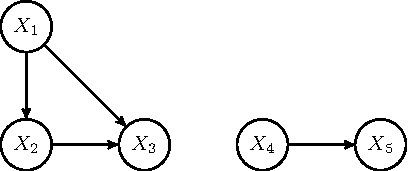
\includegraphics[keepaspectratio]{VA_generali_files/figure-pdf/unnamed-chunk-20-1.pdf}}

}

\caption{Rete bayesiana per \(5\) variabili, con due componenti connesse
(e quindi due variabili congiunte indipendenti)}

\end{figure}%

In generale, se arriva nuova informazione, la rete andrebbe ricostruita,
ma vi è una eccezione importante, ossia quando si condiziona
ulteriormente ad una informazione del tipo
\[ \cur{ X_j = x_j}_{i \in J}\] per qualche sottoinsieme di
variabili\footnote{attenzione: è importante che l'informazione riguardi
  la conoscenza esatta del valore delle \(X_j\), ossia \(X_j = x_j\), e
  non eventi del tipo \(X_j \in U_j\), altrimenti il discorso non vale.}.
Per costruire la rete bayesiana associata alla nuova informazione, è
sufficiente rimuovere dal grafo i nodi corrispondenti alle variabili
\(X_j\), e tutti gli archi da essi uscenti (che puntano ai ``figli'' di
\(X_j\)). Gli archi entranti in ciascun nodo corrispondente ad \(X_j\)
invece vanno sostituiti con archi che collegano tra loro tutti i nodi da
cui partivano (ossia i ``genitori'' di \(X_j\)), orientandoli secondo
l'ordinamento fissato sulle variabili (questo serve anche a evitare che
vi siano cicli nella rete bayesiana). Dopo questa trasformazione,
possiamo ricordare che a ciascuna componente connessa corrisponde una
variabile congiunta, e che le variabili associate a componenti diverse
sono indipendenti (rispetto alla informazione \(I\) e
\(\cur{ X_j = x_j}_{i \in J}\)).

Si considerino le variabili dell'Esempio
\textbf{?@exm-rete\_bayes\_lambda\_T} e si condizioni rispetto alla
variabile \(\Lambda\). Le variabili \(T_1\), \(T_2\), \(T_3\), \(T_4\)
diventano tra loro indipendenti, e la rete bayesiana è ottenuta
semplicemente rimuovendo il nodo relativo a \(\Lambda\) e tutti gli
archi da esso uscenti.

\begin{figure}[H]

{\centering \pandocbounded{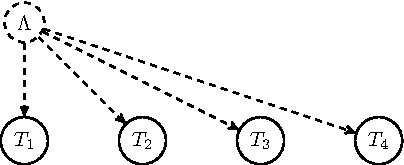
\includegraphics[keepaspectratio]{VA_generali_files/figure-pdf/unnamed-chunk-21-1.pdf}}

}

\caption{Condizionando rispetto a \(\Lambda\) si trova la rete con il
nodo rimosso.}

\end{figure}%

Si consideri invece la rete Bayesiana dell'esempio
\textbf{?@exm-rete\_bayesiana\_X\_gX}. Condizionando rispetto ad
\(Y=g(X_1, X_2, X_3)\), per ottenere la nuova rete dobbiamo collegare
tra loro tutti i nodi dei ``genitori'' di \(Y\), ossia \(X_1\), \(X_2\),
\(X_3\) (lo facciamo nell'ordine naturale per evitare cicli).
Intuitivamente è chiaro che, se conosciamo \(Y\), ad esempio nel caso
\(Y = X_1+X_2+X_3\), le variabili saranno tutt'altro che indipendenti.

\begin{figure}[H]

{\centering \pandocbounded{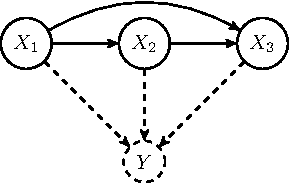
\includegraphics[keepaspectratio]{VA_generali_files/figure-pdf/unnamed-chunk-22-1.pdf}}

}

\caption{La rimozione di \(Y\) induce nuovi archi tra le \(X_i\)}

\end{figure}%

Si consideri la rete bayesiana rappresentata in figura. Condizionando
rispetto ad \(Y\), si ottiene che \(X\) e \(Z\) sono indipendenti.
Rivedremo nel Capitolo Capitolo~\ref{sec-markov} questa rete come un
semplice esempio di catena di Markov.

\begin{figure}[H]

{\centering \pandocbounded{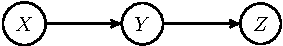
\includegraphics[keepaspectratio]{VA_generali_files/figure-pdf/unnamed-chunk-23-1.pdf}}

}

\caption{Le variabili \(X\) e \(Z\) sono condizionatamente indipendenti
sapendo \(Y\).}

\end{figure}%

A partire da una rete bayesiana, è quindi possibile ottenere la rete
condizionata all'informazione, \(\cur{X_j = x_j}_{j \in J}\), e quindi
la densità congiunta delle variabili rimanenti.

\subsection{Esercizi}\label{esercizi-15}

A partire dalla rete bayesiana in figura, si ottengano le reti
corrispondenti all'informazione condizionata a ciascun possibile
sottoinsieme delle variabili e si discuta quali variabili sono
condizionatamente indipendenti.

\begin{figure}[H]

{\centering \pandocbounded{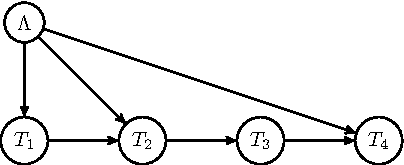
\includegraphics[keepaspectratio]{VA_generali_files/figure-pdf/unnamed-chunk-24-1.pdf}}

}

\caption{Rete bayesiana tra \(5\) variabili}

\end{figure}%

\section{Cenni ai metodi numerici}\label{sec-numerics}

I risultati introdotti finora, riguardanti le variabili aleatorie, in
particolare la formula di Bayes, permettono almeno in linea teorica di
studiare in modo rigoroso moltissimi problemi concreti, in particolare
qualora si possano ridurre a calcolare la densità (discreta o continua)
di una variabile aleatoria \(Y\) (i ``parametri'' di un modello del
problema), sulla base di informazione \(I\) inizialmente disponibile a
cui si aggiunge un'informazione associata all'osservazione di una
variabile \(X\) (i ``dati'' del modello), ovviamente rispetto alla quale
\(Y\) non sia indipendente. Abbiamo infatti già visto diversi esempi in
cui l'applicazione diretta della formula di Bayes (ad esempio, nel caso
continuo) \[ p(Y = y |  I, X=x) \propto p(Y=y|I) p( X=x| I, Y=y)\]
permette di giustificare risultati riguardanti semplici situazioni, come
ad esempio nel modello delle estrazioni dall'urna, in cui i
``parametri'' sono quantità relative allo stato dell'urna e i ``dati''
provengono dalle osservazioni delle estrazioni.

Dovrebbe anche essere evidente dagli stessi esempi che i metodi che
abbiamo introdotto, sono generalizzabili in linea teorica a modelli
arbitrariamente complessi: si pensi ad una rete bayesiana con tantissimi
nodi e connessioni, in cui ``dati'' osservati \(X\) corrispondono alla
variabile congiunta associata ad una famiglia di nodi, e si chiede di
determinare la densità dei ``parametri'' \(Y\), la congiunta associata
ai nodi rimanenti. Al crescere della numerosità dei dati e dei
parametri, ci si scontra tuttavia con il problema di \emph{calcolare} o
almeno approssimare in modo computazionalmente efficiente una densità
congiunta in uno spazio \(\R^d\) di dimensione estremamente elevata
(diciamo dell'ordine dei parametri). Anche limitandosi alla stima di
massimo a posteriori (o quella di massima verosimiglianza) \(y_{\mle}\),
che fornisce comunque una informazione utile su \(Y\), si incontra il
problema di massimizzare una funzione di \(y\), quindi di nuovo in uno
spazio \(\R^d\) di dimensione molto elevata. Anche la numerosità dei
dati \(X=x\) diventa problematica, ossia se \(X \in \R^D\) con \(D\)
estremamente grande: diventa praticamente impossibile anche solo
``definire'' analiticamente la funzione di verosimiglianza
\(p(X=x| I, Y=y)\), e quindi operare su di essa (ad esempio trovare la
stima di massima verosimiglianza).

Questo problema era evidente ancor di più prima dell'uso dei computer, e
classicamente era affrontato introducendo particolari densità a priori,
in base alle specifiche funzioni di verosimiglianza in un problema, in
modo che i calcoli delle densità a posteriori fossero analiticamente
trattabili. Tali scelte speciali di densità a priori sono dette
\emph{coniugate}\footnote{\url{https://it.wikipedia.org/wiki/Distribuzione_a_priori_coniugata}}
e sono ancora utili come particolari esempi e per situazioni semplici,
ma limitano molto l'applicabilità del metodo. Inoltre non risolvono il
problema quando comunque la numerosità delle osservazioni \(X\) diventa
intrattabile.

In \(n\) esperimenti indipendenti, ciascuno con probabilità di successo
\(Y =y\in (0,1)\), il numero \(X\) di successi ha una densità binomiale
di parametri \((n,y)\), pertanto se si è interessati a stimare \(Y\)
dalle osservazioni di \(X\), la verosimiglianza è
\[  L(Y = y; X =k) = P(X=k | Y = y) = {n \choose k} y^k (1-y)^{n-k}.\]
Se la densità di \(Y\) a priori è della famiglia \emph{Beta} di
parametri \(\alpha\), \(\beta>0\), ossia
\[ p( Y = y) \propto y^{\alpha-1} (1-y)^{\beta-1},\] (per
\(y \in (0,1)\) e zero altrimenti) allora la densità a posteriori avendo
osservato \(X=k\) successi è ancora dello stesso tipo, con parametri
\(\alpha+k\), \(\beta+n-k\),
\[ p(Y= y| X=k) \propto y^{\alpha+k-1} (1-y)^{\beta+n-k-1}.\]

Negli anni sono state introdotte e perfezionate molteplici tecniche
numeriche che cercano di superare queste difficoltà, e la ricerca in
questo ambito è estremamente attuale e rilevante. Volendo quindi
accennare ad alcuni degli approcci principali, essi si possono dividere
in due gruppi, secondo l'obiettivo che si pongono: approssimare tutta la
densità a posteriori di \(Y\), oppure determinarne solamente la stima di
massima verosimiglianza \(y_{\mle}\) (o di massimo a posteriori).

Nel primo caso, il problema consiste nell'approssimare una densità (di
solito continua) in uno spazio di dimensione alta (anche la variante
discreta comunque è importante, qualora si voglia ridurre la numerosità
dei possibili valori). Negli esempi che abbiamo considerato, ci siamo
limitati ad approssimare la densità valutandola in una griglia di punti
equispaziati. È evidente tuttavia che questa scelta non è ottimale: vi
sono regioni dove la densità è bassa e quindi sono poco rilevanti per
l'approssimazione, mentre dove la densità è alta dovremmo viceversa
infittire la griglia. In generale, il problema di approssimare una
densità continua con un'opportuna densità discreta è detto di
\emph{quantizzazione}, e vi sono diversi algoritmi per ottenere
soluzioni in modo efficace. Uno molto popolare nell'ambito della
statistica bayesiana è il cosiddetto \emph{metodo Monte Carlo} (più
precisamente i metodi \emph{Markov chain Monte Carlo} MCMC) in cui si
``simulano'' al computer un gran numero di variabili aleatorie
indipendenti tutte con stessa densità (quella da approssimare). I valori
ottenuti da tali simulazioni sostituiscono quindi la griglia di punti
equispaziati. Questo fatto è una conseguenza dell'intepretazione della
probabilità come frequenza (la legge dei grandi numeri), che dal punto
di vista matematico è un teorema come vedremo nel Capitolo
Capitolo~\ref{sec-limite}.

\begin{remark}
In R vi sono diverse librerie dedicate ai metodi Monte Carlo con
applicazioni alla statistica bayesiana per l'approsimazione delle
densità a posteriori. Due sono JAGS e Stan (che poi sono dei veri e
propri linguaggi a sé, quindi non per ragioni di tempo non li
illustreremo).
\end{remark}

Nel secondo caso, ossia la determinazione della stima di massima
verosimiglianza \(y_{\mle}\), si ricade in un contesto più ampio che è
quello dell'ottimizzazione, ossia la determinazione di punti (e valori)
di massimo o minimo di funzioni. Vi sono tantissimi algoritmi generali,
molti dei quali sfruttano il calcolo in più variabili (nel caso appunto
in cui \(Y \in \R^d\)), come ad esempio quelli di ascesa gradiente (o
discesa se l'obiettivo è un minimo invece di un massimo). Qui l'idea di
base è di avvicinarsi a \(y_{\mle}\) compiendo dei piccoli ``passi'' in
ogni punto verso la direzione in cui la funzione aumenta maggiormente
(appunto data dal gradiente della funzione nel punto). Il problema
principale qui è che la ``passeggiata'' si potrebbe bloccare in un
massimo locale (e non globale). Vi sono diversi metodi generali, spesso
``probabilistici'' come il \emph{simulated annealing} che cercano di
risolvere questa difficoltà.

In R le funzioni \texttt{nlm()} e \texttt{optim()} permettono di usare
diversi metodi per l'ottimizzazione di funzioni (ossia la determinazione
di minimi o massimi). Vediamo un esempio di applicazione.

Consideriamo le densità dell'Esempio \textbf{?@exm-bayes-continuo}.
Usando il comando \texttt{optim()} determiniamo numericamente la stima
di massmia verosimiglianza per la frazione di palline rosse.

\begin{Shaded}
\begin{Highlighting}[]
\CommentTok{\# Per determinare numericamente la stima di massima verosmiglianza definiamo come  funzione da minimizzare l\textquotesingle{}opposto del logaritmo della  verosimiglianza:}

\NormalTok{log\_likelihood }\OtherTok{=} \ControlFlowTok{function}\NormalTok{(x)\{}
  \SpecialCharTok{{-}}\FunctionTok{log}\NormalTok{( }\FunctionTok{dbinom}\NormalTok{(}\DecValTok{3}\NormalTok{, }\DecValTok{10}\NormalTok{, x) )}
\NormalTok{\}}


\CommentTok{\# determiniamone il punto di minimo la funzione optim(), specificando un valore iniziale 1/2 per il metodo iterativo e un intervallo di valori deltax,1 {-}deltax.}

\NormalTok{deltax}\OtherTok{=}\FloatTok{0.01}

\FunctionTok{plot}\NormalTok{(}\FunctionTok{seq}\NormalTok{(}\DecValTok{0}\NormalTok{,}\DecValTok{1}\NormalTok{, deltax), }\FunctionTok{log\_likelihood}\NormalTok{(}\FunctionTok{seq}\NormalTok{(}\DecValTok{0}\NormalTok{,}\DecValTok{1}\NormalTok{, deltax)), }\AttributeTok{col=}\NormalTok{miei\_colori[}\DecValTok{1}\NormalTok{], }\AttributeTok{lwd=}\DecValTok{3}\NormalTok{, }\AttributeTok{type=}\StringTok{\textquotesingle{}l\textquotesingle{}}\NormalTok{, }\AttributeTok{xlab=}\StringTok{\textquotesingle{}{-}log(L)\textquotesingle{}}\NormalTok{, }\AttributeTok{ylab=}\StringTok{\textquotesingle{}\textquotesingle{}}\NormalTok{)}
\end{Highlighting}
\end{Shaded}

\begin{center}
\pandocbounded{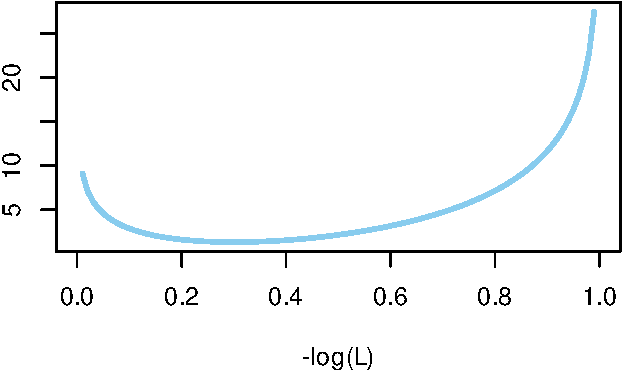
\includegraphics[keepaspectratio]{VA_generali_files/figure-pdf/unnamed-chunk-25-1.pdf}}
\end{center}

\begin{Shaded}
\begin{Highlighting}[]
\NormalTok{x\_mle }\OtherTok{=} \FunctionTok{optim}\NormalTok{( }\DecValTok{1}\SpecialCharTok{/}\DecValTok{2}\NormalTok{, log\_likelihood, }\AttributeTok{method=}\StringTok{"L{-}BFGS{-}B"}\NormalTok{, }\AttributeTok{lower=}\NormalTok{deltax, }\AttributeTok{upper =}\DecValTok{1}\SpecialCharTok{{-}}\NormalTok{deltax)}

\CommentTok{\#il parametro trovato dal metodo è}

\NormalTok{x\_mle}\SpecialCharTok{$}\NormalTok{par}
\end{Highlighting}
\end{Shaded}

\begin{verbatim}
[1] 0.3000006
\end{verbatim}

\begin{Shaded}
\begin{Highlighting}[]
\CommentTok{\# da confrontare con quello teorico 3/10}
\end{Highlighting}
\end{Shaded}

Concludiamo notando che vi sono anche casi di metodi ``misti''. Spesso
la variabile \(Y\) è interpretata come una variabile congiunta
\[Y = (Y_{\operatorname{par}}, Y_{\operatorname{hid}}),\] in cui la
prima marginale sono propriamente i ``parametri'' che si vogliono
stimare, mentre la seconda sono variabili ``nascoste'' (in inglese
\emph{latent variables}) che non interessano direttamente (ma neppure
sono i dati osservati \(X\)). La formula per la densità della marginale
diventa in questo caso
\[ p(Y_{\operatorname{par}} = y | I, X=x)= \int p(Y_{\operatorname{par}} = y | I, X=x, Y_{\operatorname{hid}} =z) p(Y_{\operatorname{hid}} = z | I, X=x) dz,\]
dove l'integrale si estende a tutti i possibili valori delle variabili
nascoste, possibilmente di dimensione molto grande. Inoltre la formula
sopra richiede di calcolare (o almeno stimare) la densità a posteriori
delle variabili nascoste. Per superare queste difficoltà è possibile
limitarsi alla determinazione della stima di massima verosimiglianza per
i parametri (quindi di \(Y_{\operatorname{par}}\)) utilizzando algoritmi
che ``alternano'' l'uso di metodi del primo caso con metodi del secondo
caso (il più popolare tra questi è l'algoritmo EM).

\subsection{Esercizi}\label{esercizi-16}

Usare la funzione \texttt{rbinom()} per simulare una variabile avente
densità binomiale. Osservare che la frequenza dei valori osservati tende
alla probabilità per un grande numero di simulazioni.

Usare la funzione \texttt{optim()} per calcolare numericamente
\[ \arg \min \cur{ (x-1)^2 + (y-2)^2 - xy : (x,y ) \in \R^2}.\]

\section{Problemi}\label{problemi-1}

Si considerino \(10\) variabili aleatorie \(X_1\), \ldots, \(X_{10}\)
indipendenti tra loro, tutte con densità continua uniforme su un
intervallo \([a,b] \subseteq \R\). Si ponga
\(X=(X_1, X_2, \ldots, X_{10})\).

\begin{enumerate}
\def\labelenumi{\arabic{enumi}.}
\tightlist
\item
  Supponendo che \(a\), \(b\) non siano noti, si determinino le stime di
  massima verosimiglianza \(a_{\mle}\), \(b_{\mle}\) avendo osservato
  dei valori \(X=(x_1, \ldots, x_{10})\).
\item
  Supponendo invece che \(a=0\) sia noto, si ponga invece \(B=b\) una
  variabile aleatoria \emph{a priori} (ossia prima di osservare le
  \(X_i\)) anch'essa uniforme su un intervallo \([0,10]\). Si osservano
  poi i valori \[ X=(1,3,5,6,3,3,5,8,7,1),\] determinare la densità di
  \(B\) a posteriori.
\end{enumerate}

Un'urna contiene una frazione \(X\) di palline rosse (le rimanenti sono
blu), e si suppone inizialmente che \(X\) sia distribuita uniformemente
su \([0,1]\). Si effettuano poi estrazioni con rimpiazzo dall'urna.

\begin{enumerate}
\def\labelenumi{\arabic{enumi}.}
\item
  Avendo osservato in \(n\) estrazioni una precisa sequenza contenente
  \(r\) palline rosse e le rimanenti \(n-r\) blu, scrivere la densità a
  posteriori di \(X\) e calcolare la stima di massimo a posteriori.
\item
  Dopo aver osservato \(n\) estrazioni di cui \(r\) palline rosse,
  calcolare la probabilità che all'estrazione \(n+1\) si estragga una
  pallina rossa.
\end{enumerate}

Si considerino due variabili \(X_1\), \(X_2\) indipendenti aventi legge
Poisson di parametri \(\lambda_1= 10\), \(\lambda_2=3\). Supponendo di
osservare che \(X_1+X_2=12\) determinare la densità di \(X_1\) e
calcolare la stima di massimo a posteriori.

Un segnale è trasmesso tramite una stringa di bit (ossia cifre binarie
\(0\) oppure \(1\)) attraverso un canale di comunicazione. Ciascuna
cifra trasmessa è affetta da un rumore che ha il seguente effetto: se si
trasmette \(0\), allora si riceve \(1\) con probabilità \(f_0\), se si
trasmette \(1\) allora si riceve \(0\) con probabilità \(f_1\). Tutto
ciò avviene per ciascuna cifra trasmessa, indipendentemente dalle altre.
I parametri \(f_0\) ed \(f_1\) non sono completamente noti, ma hanno
densità continue a priori
\[ P( F_0 = f_0 ) \propto f_0(1-f_0)^{9}, \quad P( F_1 = f_1 ) \propto f_1^4(1-f_1)^{6}.\]
Prima di trasmettere il segnale, che consiste di un solo bit, ci si è
accordati nel trasmettere una sequenza di controllo che consiste di
\(10\) zeri ripetuti seguiti da \(10\) uno ripetuti, in modo da rendersi
conto se il rumore è eccessivo. Dal punto di vista del ricevente, il
segnale consiste in un bit casuale con probabilità uniforme.

\begin{enumerate}
\def\labelenumi{\arabic{enumi}.}
\item
  Supponendo che il ricevente trascuri completamente la sequenza di
  controllo, calcolare la probabilità che riceva il segnale
  correttamente.
\item
  Supponendo che invece il ricevente ottenga nella sequenza di controllo
  \(10\) zeri seguiti da \(5\) uno e altri \(5\) zeri, come cambia la
  probabilità che riceva il segnale correttamente?
\end{enumerate}

\bookmarksetup{startatroot}

\chapter{Indicatori caratteristici}\label{indicatori-caratteristici}

In questo capitolo studiamo le principali \emph{quantità} che permettono
di sintetizzare la legge di una variabile aleatoria (reale o
vettoriale), concentrandoci in particolare sugli indicatori di posizione
(o centralità) di dispersione (o variabilità) e di correlazione.

\begin{itemize}
\item
  Nella Sezione Sezione~\ref{sec-cdf}, introduciamo la funzione di
  ripartizione (o distribuzione cumulata) e la funzione di sopravvivenza
  per variabili aleatorie reali.
\item
  La Sezione Sezione~\ref{sec-mediana} è dedicata all'inversa della
  funzione di ripartizione, la funzione quantile, che permette di
  definire anche il concetto di mediana di una distribuzione.
\item
  Nella Sezione Sezione~\ref{sec-media} definiamo il valor medio, uno
  degli indicatori di posizione più importanti ed utilizzati, anche per
  via delle proprietà che ne agevolano il calcolo in molte situazioni.
\item
  La Sezione Sezione~\ref{sec-varianza} presenta l'indice di variabilità
  più comune, la varianza (e la deviazione standard) con le sue
  proprietà.
\item
  Nella Sezione Sezione~\ref{sec-covarianza} introduciamo la covarianza
  tra due variabili aleatorie, passando così dal caso reale al caso
  vettoriale.
\item
  La Sezione Sezione~\ref{sec-mgf} presenta il concetto generale di
  momento di una variabile per approssimare il calcolo dei valori
  attesi, e la funzione generatrice dei momenti (collegata alla
  trasformata di Laplace della densità)
\item
  La Sezione Sezione~\ref{sec-caratteristica} si occupa invece della
  trasformata di Fourier della densità, che è detta in questo contesto
  funzione caratteristica di una variabile aleatoria.
\item
  Concludiamo il capitolo accennando nella Sezione
  Sezione~\ref{sec-entropia} al concetto di entropia di una densità, che
  è fondamentale in molti ambiti della teoria dell'informazione, ma può
  essere utile anche come indicatore di dispersione o per stabilire
  opportune probabilità a priori (tramite il principio di massima
  entropia).
\end{itemize}

\section{Funzione cumulativa}\label{sec-cdf}

Data una variabile aleatoria \(X\) a valori in \(\R\), abbiamo descritto
efficacemente la sua legge (rispetto ad una informazione nota \(I\))
tramite la densità discreta oppure continua.

In molti casi si è semplicemente interessati a conoscere la probabilità
che \(X\) assuma valori ``grandi''.

Per fare un esempio dal mondo della finanza, sia \(X\) la quantità di
denaro che un investitore potrebbe guadagnare (se positiva) o perdere
(se negativa) in una fissata data futura, a seconda dell'andamento del
mercato: di sicuro l'interesse principale per l'investitore sarà di
valutare la probabilità di \(\cur{ X > x}\) (per capire quanto
guadagnerà), oppure la negazione \(\cur{X \le x}\) (per capire quanto
perderà).

Partendo da questa osservazione, si introducono due funzione
strettamente collegate:

\begin{enumerate}
\def\labelenumi{\arabic{enumi}.}
\item
  la \textbf{funzione di ripartizione} (o funzione cumulativa, in
  inglese \emph{cumulative distribution function}, \(\CDF\),) di \(X\),
  definita come la funzione che ad ogni possibile valore \(x \in \R\)
  associa la probabilità che \(X \le x\),
  \[ x \mapsto \CDF_X(x) = P(X \le x), \] a volte indicata anche
  semplicemente come \(F_X\), ma è una notazione poco evocativa che
  eviteremo.
\item
  la \textbf{funzione di sopravvivenza} (in inglese \emph{survival
  function}) di \(X\), definita invece come la funzione
  \[ x \mapsto \SUR_X(x) = P(X>x),\] a volte indicata anche solo \(S_X\)
  (ma eviteremo questa notazione).
\end{enumerate}

\begin{remark}
In entrambe le definizioni sopra abbiamo sottointeso la dipendenza della
probabilità dall'informazione nota \(I\). Volendo invece indicare la
dipendenza dall'informazione \(I\), possiamo scrivere \(\CDF_{X|I}\)
oppure \(\SUR_{X|I}\).
\end{remark}

Vi è chiaramente un legame tra le due funzioni, essendo
\(\cur{X \le x}\) e \(\cur{X>x}\), fissato un qualsiasi \(x \in \R\), un
sistema di alternative. Ne segue che, per ogni \(x \in \R\),
\[  \CDF_X(x) + \SUR_X(x) = 1,\] quindi \(\CDF_X\) o \(\SUR_X\)
contengono la stessa informazione sulla legge di \(X\).

Se la densità (discreta o continua) di \(X\) è nota, è molto semplice
calcolare la \(\CDF_X\), ricordando che
\(P(X \le x) = P(X \in (-\infty, x] )\) si ottiene sommando (o
integrando) la densità su tutti i possibili valori di \(X\) che sono
minori o uguali ad \(x\): \[ \CDF_X(x) = \begin{cases} 
\sum_{  z \le x} P(X = z ) & \text{se $X$ ha densità discreta,}\\
\int_{-\infty}^x f(z) d z & \text{ se $X$ ha densità continua.}\end{cases} (\#eq:CDF-density)\]

Possiamo quindi intepretare (almeno nel caso continuo) la \(\CDF_X(x)\)
come l'area del sottografico della densità da \(-\infty\) fino ad \(x\).

Analogamente, per la funzione di sopravvivenza, si somma (o integra) sui
valori strettamente maggiori di \(x\): \[ \SUR_X(x) = \begin{cases} 
\sum_{  z > x} P(X = z ) & \text{se $X$ ha densità discreta,}\\
\int_x ^{+\infty} f(z) d z & \text{ se $X$ ha densità continua,}\end{cases}\]

e quindi corrisponde all'area del sottografico della densità (continua)
da \(x\) a \(+\infty\).

Si consideri una variabile aleatoria \(X\) sui valori
\(E = \cur{-2,1,0,2}\) avente densità uniforme \[ P(X =i ) = 1/4.\] Il
grafico della sua densità discreta e della \(\CDF_X\), ottenuto tramite
la formula sopra (nel caso discreto) è rappresentata in figura:

\begin{Shaded}
\begin{Highlighting}[]
\CommentTok{\# possibili valori e densità discreta}
\NormalTok{valori\_X }\OtherTok{\textless{}{-}} \FunctionTok{c}\NormalTok{(}\SpecialCharTok{{-}}\DecValTok{2}\NormalTok{,}\DecValTok{0}\NormalTok{,}\DecValTok{1}\NormalTok{,}\DecValTok{2}\NormalTok{)}
\NormalTok{densita\_X }\OtherTok{\textless{}{-}} \FunctionTok{rep}\NormalTok{(}\DecValTok{1}\SpecialCharTok{/}\DecValTok{4}\NormalTok{, }\DecValTok{4}\NormalTok{)}

\CommentTok{\# iniziamo con un grafico vuoto:}


\FunctionTok{plot}\NormalTok{(}\ConstantTok{NULL}\NormalTok{, }\AttributeTok{xlab=}\StringTok{\textquotesingle{}valori\textquotesingle{}}\NormalTok{, }\AttributeTok{ylab=}\StringTok{\textquotesingle{}probabilità\textquotesingle{}}\NormalTok{, }\AttributeTok{ylim=}\FunctionTok{c}\NormalTok{(}\DecValTok{0}\NormalTok{,}\DecValTok{1}\NormalTok{), }\AttributeTok{xlim=}\FunctionTok{c}\NormalTok{(}\SpecialCharTok{{-}}\DecValTok{3}\NormalTok{,}\DecValTok{3}\NormalTok{))}

\CommentTok{\#per avere un plot su un intervallo ad esempio ({-}3,3), aggiungiamo artificialmente i due valori estremi con densità 0 (questo rende più semplice fare il plot della CDF come funzione a gradini)}

\NormalTok{valori\_X }\OtherTok{\textless{}{-}} \FunctionTok{c}\NormalTok{(}\SpecialCharTok{{-}}\DecValTok{3}\NormalTok{, valori\_X, }\DecValTok{3}\NormalTok{)}
\NormalTok{densita\_X }\OtherTok{\textless{}{-}} \FunctionTok{c}\NormalTok{(}\DecValTok{0}\NormalTok{, densita\_X, }\DecValTok{0}\NormalTok{)}


\CommentTok{\# per ottenere la funzione di ripartizione nei punti valori\_X usiamo il comando cumsum().}

\NormalTok{CDF\_X }\OtherTok{\textless{}{-}} \FunctionTok{cumsum}\NormalTok{(densita\_X)}


\CommentTok{\# aggiungiamo il grafico della CDF con il comando lines()}


\FunctionTok{lines}\NormalTok{(valori\_X, CDF\_X, }\AttributeTok{type=}\StringTok{\textquotesingle{}s\textquotesingle{}}\NormalTok{, }\AttributeTok{col=}\NormalTok{miei\_colori[}\DecValTok{2}\NormalTok{], }\AttributeTok{lwd=}\DecValTok{3}\NormalTok{)}

\CommentTok{\# infine aggiungiamo i punti corrispondenti alla densità discreta}


\FunctionTok{points}\NormalTok{( valori\_X[}\DecValTok{2}\SpecialCharTok{:}\DecValTok{5}\NormalTok{], densita\_X[}\DecValTok{2}\SpecialCharTok{:}\DecValTok{5}\NormalTok{], }\AttributeTok{col=}\NormalTok{miei\_colori[}\DecValTok{1}\NormalTok{], }\AttributeTok{pch=}\DecValTok{16}\NormalTok{, }\AttributeTok{lwd=}\DecValTok{3}\NormalTok{)}
\end{Highlighting}
\end{Shaded}

\begin{figure}[H]

{\centering \pandocbounded{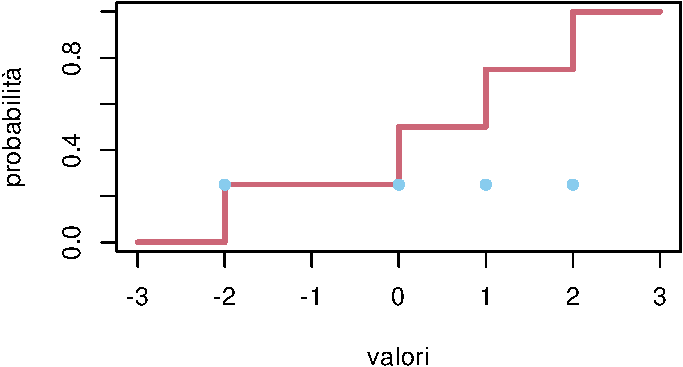
\includegraphics[keepaspectratio]{04-VA_indicatori_files/figure-pdf/unnamed-chunk-2-1.pdf}}

}

\caption{densità uniforme discreta e CDF}

\end{figure}%

Ad essere precisi, il grafico della \(CDF_X\) non dovrebbe rappresentare
i segmenti verticali nei punti di salto (il valore della \(\CDF_X\) è
soltanto l'estremo più alto).

Si consideri una variabile aleatoria \(X\) avente densità uniforme
continua nell'intervallo \([-2,2]\), ossia, per \(x \in [-2,2]\),
\[ p(X =x ) = 1/4.\] Il grafico della sua densità continua e della
\(\CDF_X\), ottenuto tramite la formula sopra (nel caso continuo) è
rappresentata in figura:

\begin{Shaded}
\begin{Highlighting}[]
\CommentTok{\# possibili valori e densità continua}
\NormalTok{deltax }\OtherTok{=} \FloatTok{0.01}
\NormalTok{valori\_X }\OtherTok{\textless{}{-}} \FunctionTok{seq}\NormalTok{(}\SpecialCharTok{{-}}\DecValTok{3}\NormalTok{,}\DecValTok{3}\NormalTok{, }\AttributeTok{by=}\NormalTok{deltax)}
\NormalTok{densita\_X }\OtherTok{\textless{}{-}}\NormalTok{ valori\_X}\SpecialCharTok{*}\DecValTok{0} \SpecialCharTok{+}\NormalTok{ (valori\_X}\SpecialCharTok{\textgreater{}{-}}\DecValTok{2} \SpecialCharTok{\&}\NormalTok{ valori\_X }\SpecialCharTok{\textless{}}\DecValTok{2}\NormalTok{)}\SpecialCharTok{*}\DecValTok{1}\SpecialCharTok{/}\DecValTok{4}

\CommentTok{\# plottiamo prima i valori della densità }

\FunctionTok{plot}\NormalTok{(valori\_X, densita\_X, }\AttributeTok{type=}\StringTok{\textquotesingle{}l\textquotesingle{}}\NormalTok{, }\AttributeTok{col=}\NormalTok{miei\_colori[}\DecValTok{1}\NormalTok{], }\AttributeTok{xlab=}\StringTok{\textquotesingle{}valori\textquotesingle{}}\NormalTok{, }\AttributeTok{ylab=}\StringTok{\textquotesingle{}\textquotesingle{}}\NormalTok{, }\AttributeTok{ylim=}\FunctionTok{c}\NormalTok{(}\DecValTok{0}\NormalTok{,}\DecValTok{1}\NormalTok{), }\AttributeTok{xlim=}\FunctionTok{c}\NormalTok{(}\SpecialCharTok{{-}}\DecValTok{3}\NormalTok{,}\DecValTok{3}\NormalTok{), }\AttributeTok{lwd=}\DecValTok{3}\NormalTok{)}


\CommentTok{\# per ottenere la funzione di ripartizione nei punti valori\_X usiamo il comando cumsum() moltiplicando poi per deltax (per approssimare l\textquotesingle{}integrale come somma di Riemann)}

\NormalTok{CDF\_X }\OtherTok{\textless{}{-}} \FunctionTok{cumsum}\NormalTok{(densita\_X)}\SpecialCharTok{*}\NormalTok{deltax}


\CommentTok{\#aggiungiamo quindi con il comando lines()}


\FunctionTok{lines}\NormalTok{(valori\_X, CDF\_X, }\AttributeTok{type=}\StringTok{\textquotesingle{}l\textquotesingle{}}\NormalTok{, }\AttributeTok{col=}\NormalTok{miei\_colori[}\DecValTok{2}\NormalTok{], }\AttributeTok{lwd=}\DecValTok{3}\NormalTok{)}
\end{Highlighting}
\end{Shaded}

\begin{figure}[H]

{\centering \pandocbounded{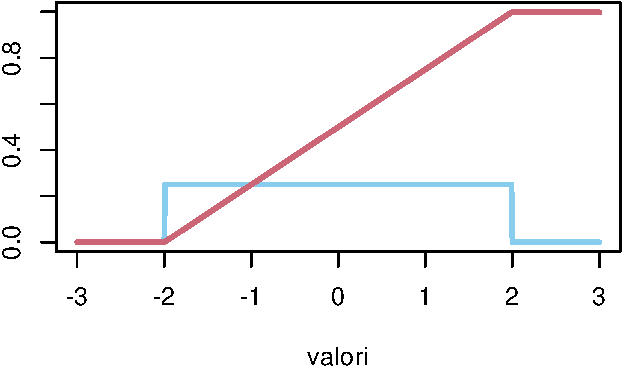
\includegraphics[keepaspectratio]{04-VA_indicatori_files/figure-pdf/unnamed-chunk-3-1.pdf}}

}

\caption{densità uniforme continua e CDF}

\end{figure}%

Osservando i grafici ottenuti, deduciamo alcune semplici proprietà della
\(\CDF\):

\begin{enumerate}
\def\labelenumi{\arabic{enumi}.}
\tightlist
\item
  vale \(\CDF_X(x) \in [0,1]\), essendo una probabilità.
\item
  la funzione \(x \mapsto \CDF_X(x)\) è crescente (ma non strettamente):
  se \(x < z\), allora \(\CDF_X(x) \le \CDF_X(z)\), per la monotonia
  della probabilità: ogni volta che \(\cur{X \le x}\) è vero, segue che
  \(\cur{X \le z}\) è pure vero.
\item
  vale \(\CDF_X(-\infty) = 0\) e \(\CDF_X(+\infty)=1\) (nel senso di
  limiti opportuni): negli esempi si ha addirittura \(\CDF_X(-3)=0\) e
  \(\CDF_X(3)=1\), ma questo dipende dalle densità considerate.
\item
  Nel caso di variabili con densità discreta, la \(\CDF_X\) è una
  funzione costante a tratti, mentre nel caso di variabili con densità
  continua, la \(\CDF_X\) è una funzione continua.
\end{enumerate}

Per la funzione \(\SUR\), valgono proprietà analoghe, fatte le opportune
considerazioni: in particolare, la funzione è decrescente e vale
\(\SUR_X(-\infty) = 1\) mentre \(\SUR_X(+\infty) = 0\).

Si consideri una variabile aleatoria \(X\) con densità esponenziale di
parametro \(\lambda>0\). Si trova che
\[ \SUR_X(x) = \int_x^\infty \lambda e^{-\lambda z} d z = e^{-\lambda x},\]
mentre \[ \SUR_X(x) = 1- e^{-\lambda x}.\]. Nel caso \(\lambda = 1/2\),
il grafico della densità, funzione di ripartizione e di sopravvivenza
sono tracciati in figura.

\begin{Shaded}
\begin{Highlighting}[]
\NormalTok{deltax }\OtherTok{\textless{}{-}} \FloatTok{0.01}
\NormalTok{valori\_X }\OtherTok{\textless{}{-}} \FunctionTok{seq}\NormalTok{(}\SpecialCharTok{{-}}\DecValTok{1}\NormalTok{, }\DecValTok{3}\NormalTok{, }\AttributeTok{by=}\NormalTok{deltax)}
\NormalTok{lambda }\OtherTok{\textless{}{-}}\DecValTok{1}\SpecialCharTok{/}\DecValTok{2}
\CommentTok{\# usiamo direttamente i comandi dexp() e pexp() per la densità e CDF esponeziale}

\NormalTok{densita\_X }\OtherTok{\textless{}{-}} \FunctionTok{dexp}\NormalTok{(valori\_X, lambda)}
\NormalTok{CDF\_X }\OtherTok{\textless{}{-}} \FunctionTok{pexp}\NormalTok{(valori\_X, lambda)}
\NormalTok{SUR\_X }\OtherTok{\textless{}{-}} \DecValTok{1}\SpecialCharTok{{-}}\NormalTok{CDF\_X}

\FunctionTok{plot}\NormalTok{( valori\_X, densita\_X, }\AttributeTok{type=}\StringTok{\textquotesingle{}l\textquotesingle{}}\NormalTok{, }\AttributeTok{col=}\NormalTok{miei\_colori[}\DecValTok{1}\NormalTok{], }\AttributeTok{ylim=}\FunctionTok{c}\NormalTok{(}\DecValTok{0}\NormalTok{,}\DecValTok{1}\NormalTok{), }\AttributeTok{xlab=}\StringTok{\textquotesingle{}valori\textquotesingle{}}\NormalTok{, }\AttributeTok{ylab=}\StringTok{\textquotesingle{}\textquotesingle{}}\NormalTok{, }\AttributeTok{lwd=}\DecValTok{3}\NormalTok{)}
\FunctionTok{lines}\NormalTok{( valori\_X, CDF\_X, }\AttributeTok{col=}\NormalTok{miei\_colori[}\DecValTok{2}\NormalTok{], }\AttributeTok{lwd=}\DecValTok{3}\NormalTok{, )}
\FunctionTok{lines}\NormalTok{( valori\_X, SUR\_X, }\AttributeTok{co=}\NormalTok{miei\_colori[}\DecValTok{3}\NormalTok{], }\AttributeTok{lwd=}\DecValTok{3}\NormalTok{)}

\FunctionTok{legend}\NormalTok{(}\StringTok{\textquotesingle{}topright\textquotesingle{}}\NormalTok{, }\AttributeTok{fill=}\NormalTok{miei\_colori[}\DecValTok{1}\SpecialCharTok{:}\DecValTok{3}\NormalTok{], }\FunctionTok{c}\NormalTok{(}\StringTok{"densità"}\NormalTok{, }\StringTok{"CDF"}\NormalTok{, }\StringTok{"SUR"}\NormalTok{), }\AttributeTok{cex=}\FloatTok{0.8}\NormalTok{)}
\end{Highlighting}
\end{Shaded}

\begin{figure}[H]

{\centering \pandocbounded{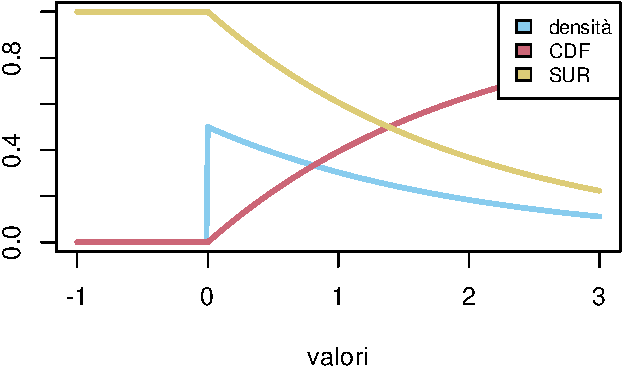
\includegraphics[keepaspectratio]{04-VA_indicatori_files/figure-pdf/unnamed-chunk-4-1.pdf}}

}

\caption{densità, \(\CDF_X\) e \(\SUR_X\) di una variabile \(X\) con
densità esponenziale di parametro \(\lambda=1/2\).}

\end{figure}%

È naturale a questo punto porsi la seguente domanda: possiamo
ricostruire la densità di \(X\) (discreta o continua) se disponiamo
della \(\CDF_X\)? la risposta è affermativa e basta invertire la
\textbf{?@eq-CDF-density}. Nel caso discreto, si trova semplicemente che
la densità discreta è non nulla solo nei valori \(x\in \R\) in cui la
\(\CDF_X(x)\) ha un salto, e il valore della densità in quel punto è
proprio l'ampiezza del salto. Nel caso di densità continua, per
invertire la formula \[ \int_{-\infty}^x p(X=z)dz = \CDF_X(x)\] è
sufficiente applicare il teorema fondamentale del calcolo integrale, e
quindi derivare la \(\CDF_X\) per ottenere la densità:
\[ \frac{d}{dx} \CDF_X(x) = p(X=x).\] (nei punti in cui \(\CDF_X\) è
derivabile)

Per la \(\SUR_X\), è sufficiente cambiare di segno alle quantità
ottenute, ossia intepretare l'ampiezza assoluta dei salti nel caso
discreto, mentre, nel caso continuo, si ottiene
\[ - \frac{d}{dx} \SUR_X(x) = p(X=x).\]

\begin{remark}
Vi sono variabili aleatorie \(X\) né discrete né continue. In tal caso
si può ancora mostrare che la conoscenza della \(\CDF_X\) (o la
\(\SUR_X\)) determina completamente la legge di \(X\).
\end{remark}

\subsection{Esercizi}\label{esercizi-17}

Sia \(X\) una variabile aleatoria reale con densità continua
\emph{pari}, ossia tale che \(p(X=x)  = p(X =-x)\) per ogni
\(x \in \R\). Mostrare che \(\CDF_X(x) = \SUR_X(-x)\) per ogni
\(x \in \R\).

Tramite il comando \(R\) \texttt{pbinom()} rappresentare graficamente la
\(\CDF\) di una variabile \(X\) con densità binomiale di parametri
\((10, 1/4)\). Usando il comando \texttt{phyper()} si faccia lo stesso
per una densità ipergeometrica (si scelgano a piacere i parametri).

Può la funzione \(x\mapsto \sin(x)\), \(x \in [0, \pi/2]\) essere la
\(\CDF\) di qualche variabile aleatoria?

\section{Mediana e quantile}\label{sec-mediana}

Ricordiamo che il nostro obiettivo in questo capitolo è di definire
delle quantità che riassumano la legge di una variabile \(X\) in modo
semplice ma efficace. La \(\CDF_X\) da questo punto di vista contiene
troppa informazione, essendo praticamente equivalente ad avere la
densità di \(X\). Per ridurre tale informazione in modo efficace, ci si
può tuttavia limitare ad alcuni valori (della variabile \(X\)) speciali
determinati tramite la \(\CDF_X\), o meglio la sua inversa.

Il più semplice da definire è la \emph{mediana} di \(X\), definita come
un valore \(\bar{x} \in \R\), se esiste, tale che
\[ \CDF_X(\bar{x}) = \frac 1 2.\] Ricordando la definizione di
\(\CDF_X\), significa che
\[ P(X\le \bar{x}) = P(X> \bar{x}) =\frac 1 2,\] ossia \(\bar{x}\) è
scelta in modo che le due alternative \(\cur{X \le \bar{x}}\) e
\(\cur{X > \bar{x}}\) abbiano la stessa probabilità. La mediana è quindi
un buon indicatore di ``centralità'' per una variabile aleatoria \(X\),
simile alla moda, ma in alcuni casi più utile.

Ad esempio, se la densità di \(X\) è uniforme (diciamo su un insieme
\(E\) con un numero pari di valori), significa che metà dei valori
possibili di \(X\) sono \(\le \bar{x}\), mentre i rimanenti sono
\(>\bar{x}\). In questo caso invece una moda è uno qualsiasi dei valori
di \(E\).

Si consideri una variabile \(X\) uniforme sui \(10\) valori
\(E = \cur{0, 0.1, 0.15, 0.3, 0.4, 0.7, 0.73, 0.9, 0.95, 1.1}\). Una
mediana per \(X\) è \(\bar{x}=0.4\), ma anche un qualsiasi valore
compreso tra \(0.4\) e \(0.7\) (escluso)

Nel caso di una variabile esponenziale di parametro \(\lambda\), si
trova che
\[ 1- e^{-\lambda \bar{x}} = \frac 1 2\quad  \leftrightarrow \quad \lambda \bar{x} = \log(2),\]
ossia \[\bar{x} = \frac{\log(2)}{\lambda}.\] In questo caso la mediana è
unica. Osserviamo che la dipendenza da \(\lambda\) (a denominatore) è in
linea con le osservazioni fatte nel capitolo precedente sulla dipendenza
da \(\lambda\) della densità.

La mediana tuttavia presenta alcuni problemi: non necessariamente esiste
sempre, oppure può non essere unicamente determinata dall'equazione
sopra, infine non è facile calcolarla (si tratta di risolvere
un'equazione).

Per risolvere i primi due problemi, si introduce una inversa
generalizzata della funzione \(\CDF_X\), detta funzione \emph{quantile}
di \(X\). In effetti, l'equazione che definisce la mediana, se
\(\CDF_X\) è invertibile, darebbe \[ \bar{x} = \CDF_X^{-1}(1/2).\] Il
fatto è che la \(\CDF_X\) non è invertibile (si pensi al caso di
variabili discrete, in cui è costante a tratti): perciò si introduce la
funzione quantile di \(X\) come la funzione \[ q_X : (0,1) \to \R\] che
ad ogni possibile \(\alpha \in (0,1)\) (detto anche \emph{livello} del
quantile) associa il valore
\[ q_X(\alpha) = \min\cur{ x \in \R \, : \, \CDF_X(x) \ge \alpha},\]
detto appunto, quantile di \(X\) di livello \(\alpha\). Si può
dimostrare (noi non lo faremo) che vale, per ogni \(\alpha \in (0,1)\).
\[ \CDF_X( q_X(\alpha)) \ge \alpha\], mentre se \(X\) ha densità
continua, allora \[ \CDF_X( q_X(\alpha)) = \alpha.\]

La funzione quantile delle densità notevoli è già impostata in R,
tramite il prefisso \texttt{q} (in contrasto con \texttt{p} della CDF e
\texttt{d} per la densità). Plottiamo ad esempio il quantile della
densità binomiale (discreta) e quello della densità esponenziale
(continua).

\begin{Shaded}
\begin{Highlighting}[]
\NormalTok{n}\OtherTok{=}\DecValTok{10}
\NormalTok{p}\OtherTok{=}\DecValTok{2}\SpecialCharTok{/}\DecValTok{3}

\NormalTok{valori\_X }\OtherTok{=} \DecValTok{0}\SpecialCharTok{:}\NormalTok{n}
\NormalTok{CDF\_X }\OtherTok{=} \FunctionTok{pbinom}\NormalTok{(valori\_X, n, p)}

\NormalTok{delta\_alpha }\OtherTok{=} \FloatTok{0.01}
\NormalTok{alpha }\OtherTok{=} \FunctionTok{seq}\NormalTok{(}\DecValTok{0}\NormalTok{, }\DecValTok{1}\NormalTok{, }\AttributeTok{by=}\NormalTok{delta\_alpha)}
\NormalTok{quantile\_X  }\OtherTok{=} \FunctionTok{qbinom}\NormalTok{(alpha, n, p)}

\CommentTok{\# per visualizzare i due plot uno accanto all\textquotesingle{}altro usiamo la funzione par()}

\FunctionTok{par}\NormalTok{(}\AttributeTok{mfrow=}\FunctionTok{c}\NormalTok{(}\DecValTok{1}\NormalTok{,}\DecValTok{2}\NormalTok{))}

\FunctionTok{plot}\NormalTok{(valori\_X, CDF\_X, }\AttributeTok{type=}\StringTok{\textquotesingle{}s\textquotesingle{}}\NormalTok{, }\AttributeTok{col=}\NormalTok{miei\_colori[}\DecValTok{1}\NormalTok{], }\AttributeTok{xlab=}\StringTok{\textquotesingle{}valore\textquotesingle{}}\NormalTok{, }\AttributeTok{ylab=}\StringTok{\textquotesingle{}probabilità\textquotesingle{}}\NormalTok{, }\AttributeTok{lwd=}\DecValTok{3}\NormalTok{)}
\FunctionTok{plot}\NormalTok{(alpha, quantile\_X, }\AttributeTok{type=}\StringTok{\textquotesingle{}S\textquotesingle{}}\NormalTok{, }\AttributeTok{col=}\NormalTok{miei\_colori[}\DecValTok{2}\NormalTok{], }\AttributeTok{xlab=}\StringTok{\textquotesingle{}livello\textquotesingle{}}\NormalTok{, }\AttributeTok{ylab=}\StringTok{\textquotesingle{}valore\textquotesingle{}}\NormalTok{, }\AttributeTok{lwd=}\DecValTok{3}\NormalTok{)}
\end{Highlighting}
\end{Shaded}

\begin{figure}[H]

{\centering \pandocbounded{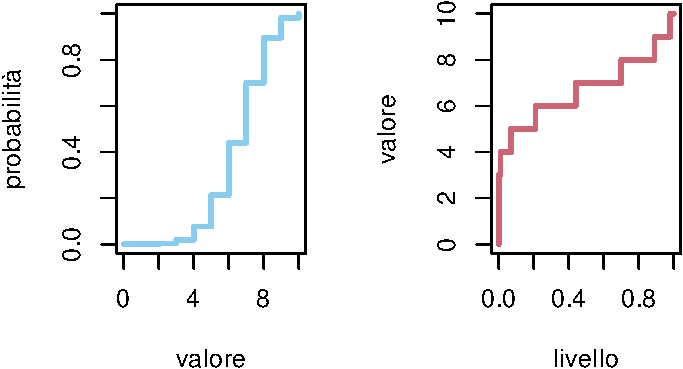
\includegraphics[keepaspectratio]{04-VA_indicatori_files/figure-pdf/unnamed-chunk-5-1.pdf}}

}

\caption{plot di \(\CDF_X\) per \(X\) binomiale (a sinistra) e quantile
funzione quantile (a destra)}

\end{figure}%

Nel caso generale, si definisce quindi la mediana di \(X\) come il
valore \(\bar{x} = q_X(1/2)\). Altri valori speciali della funzione
quantile sono i \emph{quartili}, corrispondenti ad
\(\alpha \in \cur{ 1/4, 2/4, 3/4}\) (detti il primo, secondo e terzo
quartile), i \emph{decili} e i \emph{percentili}, corrispondenti
rispettivamente ai livelli \(\alpha = k/10\), oppure \(\alpha=k/100\).
Affiancare alla mediana i quartili permette di descrivere la variabilità
della \(X\) (ossia indicare quanto i valori siano tipicamente vicini
alla mediana).

\subsection{Esercizi}\label{esercizi-18}

Calcolare e plottare la funzione quantile di una variabile \(X\) con
densità uniforme (continua) su \((a,b)\) (si può eventualmente usare la
funzione \texttt{qunif()}).

Calcolare e plottare la funzione quantile di una variabile \(X\) con
densità (Cauchy) \(p(X=x) \propto 1/(x^2+1)\) (si veda il comando
\texttt{qcauchy()}).

Sia \(X\) una variabile aleatoria a valori in \(\R\) e sia
\(g: \R \to \R\) continua e strettamente crescente. Che legame c'è tra
\(q_X\) e \(q_{g(X)}\)?

\section{Valor medio}\label{sec-media}

La mediana e le sue generalizzazioni come i quartili, decili ecc., sono
efficaci per sintetizzare le principali caratteristiche della legge di
una variabile aleatoria a valori reali. Tuttavia il loro calcolo
(teorico) non è molto agevole e pure la generalizzazione al caso di
variabili vettoriali non è del tutto evidente. In questa sezione
introduciamo invece uno degli indicatori maggiormente usati, il valor
medio (anche detta media, valore atteso o speranza matematica, in
inglese \emph{expectation} o \emph{expected value}) di una variabile
aleatoria \(X\) a valori in \(\R\), rispetto all'informazione \(I\). La
ragione principale per preferire il valor medio rispetto alla mediana è
che esso gode di molteplici proprietà, di cui la principale è la
linearità, che ne rendono il calcolo agevole in molte situazioni.
Inoltre, si generalizza in modo immediato al caso vettoriale.

Il valor medio di \(X\) consiste in una media aritmetica dei possibili
valori di \(X\), ma \emph{ponderata}, cioè pesata, tramite la densità
(discreta o continua).

Il valor medio di una variabile aleatoria \(X\) a valori in \(\R\),
condizionato ad una informazione nota \(I\) rispetto alla quale \(X\)
ammette densità (discreta o continua) è definito come il numero reale
\[ \E{ X | I} = \begin{cases} \sum_{x \in \R} x P(X = x|I ) & \text{se $X$ ha densità discreta,}\\ 
\int_{-\infty}^\infty x p(X=x|I) d x & \text{se $X$ ha densità continua.}\end{cases}\]

La notazione \(\E{X | I}\) ricalca quella di probabilità \(P(X=x|I)\), e
spesso si evita di specificare l'informazione nota \(I\).

\begin{remark}
Affinché la serie o l'integrale siano ben definiti, supporremo sempre
(tacitamente) che convergano in senso assoluto, ossia
\[ \sum_{x \in \R} |x| P(X = x|I )  < \infty  \text{ oppure } \int_{-\infty}^\infty |x| p(X=x|I) d x <\infty.\]
questo evita opportunamente dei comportamenti ``patologici'' nei
passaggi al limite. Se le serie sopra non convergono, diremo
semplicemente che il valor medio non esiste finito (o non è ben
definito). Diversamente dalla mediana, che esiste sempre (purché si
definisca come \(q_X(1/2)\)), il valor medio potrebbe non esistere.
\end{remark}

La definizione che abbiamo dato di valor medio ricalca quella fisica di
\emph{centro di massa} per una certa distribuzione di massa, solamente
che al posto della densità di massa vi è la densità di probabilità. In
effetti, per molte applicazioni in fisica il centro di massa fornisce un
utile riassunto per una distribuzione di massa.

Il calcolo analitico di un valor medio può essere un esercizio piuttosto
complicato. Dal punto di vista numerico invece è immediato (se si
dispone della densità o di una sua approssimazione).

Sia \(X\in \cur{0,1}\) la variabile indicatrice di un evento \(A\),
ossia \(\cur{X=1} = A\). La legge di \(X\) è Bernoulli di parametro
\(p = P(X=1|I) = P(A|I)\) Allora, usando la definizione nel caso
discreto,
\[ \E{X|I} = 0\cdot P(X= 0|I) + 1 \cdot P(X=1|I) = P(X=1|I) = P(A|I) = p,\]
quindi il valor medio di una (variabile con) densità discreta Bernoulli
di parametro \(p\) è proprio \(p\). Osserviamo che, eccetto i casi
limite \(p =0\), oppure \(p=1\), il valor medio non è uno dei possibili
valori di \(X\).

Sia \(X\) una variabile aleatoria uniforme continua sull'intervallo
\((a,b)\). Allora il valor medio di \(X\) è
\[  \int_a^b x \frac{1}{b-a} dx  = \frac{( b^2-a^2)}{2 (b-a)} = \frac{a+b}{2},\]
ossia il punto medio dell'intervallo. Notiamo che in questo caso il
valor medio è uno dei possibili valori e coincide con la mediana.

Sia \(X\) una variabile aleatoria con densità binomiale di parametri
\(n=10\), \(p=1/3\). Per calcolare il valor medio usando la definizione,
bisogna sommare
\[ \sum_{k=0}^{10} k {10 \choose k} \frac{1}{3^{k}} \bra{\frac{2}{3}}^{10-k}.\]
Vedremo più avanti un approccio diverso sfruttando le proprietà di
linearità del valor medio. Tuttavia è anche semplice calcolarlo
numericamente:

\begin{Shaded}
\begin{Highlighting}[]
\NormalTok{n }\OtherTok{\textless{}{-}} \DecValTok{10}
\NormalTok{p }\OtherTok{\textless{}{-}} \DecValTok{1}\SpecialCharTok{/}\DecValTok{3}

\NormalTok{valori\_X }\OtherTok{\textless{}{-}} \DecValTok{0}\SpecialCharTok{:}\NormalTok{n}
\NormalTok{densita\_X }\OtherTok{\textless{}{-}} \FunctionTok{dbinom}\NormalTok{(valori\_X, n, p)}

\NormalTok{(valor\_medio\_X }\OtherTok{\textless{}{-}} \FunctionTok{sum}\NormalTok{(valori\_X }\SpecialCharTok{*}\NormalTok{ densita\_X))}
\end{Highlighting}
\end{Shaded}

\begin{verbatim}
[1] 3.333333
\end{verbatim}

\begin{remark}
Come anticipato, ci limiteremo al calcolo (esplicito) del valor medio
nei casi in cui \(X\) ammetta densità discreta o continua. Tuttavia si
deve notare che è possibile dare una definizione generale, che non usa
la densità. Una possibile è la seguente (va però mostrato che le
definizioni coincidano):
\[ \E{X |I} = \int_0^\infty P(X>x|I) d x - \int_{-\infty}^0 P(X <x) dx, \]
supponendo che entrambi gli integrali convergano.
\end{remark}

Veniamo alle proprietà principali del valor medio, riassunte nella
seguente proposizione. Accenniamo alle dimostrazioni nei casi semplici
di variabili discrete (o continue).

La proprietà fondamentale è l'analoga della formula di disintegrazione
per la probabilità, che possiamo scrivere in termini di sistemi di
alternative o variabili aleatorie (discrete o continue).

Sia \(X\) una variabile aleatoria reale e sia \(Y \in E\) una variabile
aleatoria. 1. Se \(Y\) ha densità discreta, vale
\[ \E{X|I}= \sum_{y \in E} \E{X|I, Y=y} P(Y=y|I),\] 2. Se \(E = \R^d\) e
\(Y\) ha densità continua, vale
\[ \E{X|I} = \int_{\R^d }\E{X|I, Y=y} p(Y=y|I) dy.\]

\begin{proof}
La dimostrazione di questa proprietà è immediata, almeno nel caso
discreto, purché si ammetta di poter scambiare le serie (questo
passaggio tecnico richiede appunto la convergenza assoluta): omettendo
di specificare l'informazione \(I\), vale \[ \begin{split} 
\E{X} & = \sum_{x \in \R} x P(X=x) = \sum_{x \in \R} x \sum_{y\in E} P(X=x|Y=y)P(Y=y)\\
&\sum_{y \in E} \bra{ \sum_{x \in \R} x  P(X=x|Y=y)}P(Y=y)\\
& \sum_{y \in E} \E{X | Y=y} P(Y=y).
\end{split}\] Similmente nel caso continuo, scambiando gli integrali
(nei casi misti invece si scambiano serie e integrali).
\end{proof}

Grazie alla formula di disintegrazione, possiamo agevolmente dimostrare
ulteriori proprietà.

Siano \(X\), \(Y\) variabili aleatorie reali, e siano \(a\), \(b\),
\(c \in \R\) (non aleatorie). Allora

\begin{enumerate}
\def\labelenumi{\arabic{enumi}.}
\tightlist
\item
  (linearità) vale \(\E{aX|I} = a \E{X|I}\) e
  \(\E{X+Y|I }= \E{X|I} + \E{Y|I}\).
\item
  (monotonia) se \(P( X \ge Y|I) = 1\), allora \(\E{X|I} \ge \E{Y|I}\).
  In particolare, se \(P(X\in[a,b]|I) = 1\), allora
  \(\E{X|I} \in [a,b]\).
\item
  (diseguaglianza di Markov) se \(X\) è a valori non-negativi (rispetto
  all'informazione \(I\)), allora per ogni \(c>0\),
  \[ P(X > c|I) \le \frac{ \E{X|I}}{c}.\]
\end{enumerate}

\begin{proof}
Limitiamoci al caso di variabili con densità discreta.

\begin{enumerate}
\def\labelenumi{\arabic{enumi}.}
\item
  Per mostrare la linearità, usiamo la disintegrazione con \(X+Y\)
  invece di \(X\) e la variabile congiunta \((X,Y)\) invece di \(Y\).
  Troviamo (omettiamo \(I\) per brevità)
  \[ \begin{split} \E{X+Y} & = \sum_{(x,y)\in \R \times \R} \E{X+Y| X=x, Y=y} P(X=x, Y=y) \\
  & \sum_{(x,y)\in \R \times \R} (x+y) P(X=x, Y=y)\\
  &\sum_{x \in \R } x \sum_{y \in \R } P(X=x, Y=y) + \sum_{y \in \R } y \sum_{x \in \R } P(X=x, Y=y) \\
  & \sum_{x \in \R} x P(X=x) + \sum_{y \in \R} y P(Y=y)\end{split}\]
  dove abbiamo usato la formula per la densità delle marginali a partire
  dalla densità della variabile congiunta. La dimostrazione di
  \(\E{aX}= a \E{X}\) è analoga (disintegrando rispetto ad \(X\)).
\item
  Avendo dimostrato la linearità del valor medio, possiamo porre
  \(Z = X-Y\) e limitarci a dimostarre \(\E{Z} \ge 0\) partendo
  dall'ipotesi che \(P(Z\ge 0) = 1\). Ma allora nella definizione
  (sempre nel caso discreto) possiamo ridurre la somma agli \(z \ge 0\)
  (visto che \(P(Z = z) = 0\) se \(z<0\)),e quindi
  \[ \E{Z}=  \sum_{z \in \R} z P(Z= z) =  \sum_{z \ge 0} z P(Z=z) \ge 0,\]
  essendo ciascun termine \(z P(Z=z)\) positivo.
\item
  Consideriamo il sistema di alternative \(\cur{X<c}\),
  \(\cur{X \ge c}\) e disintegriamo:
  \[\begin{split} \E{X} & =\E{X|X<c} P(X<c) + \E{X| X \ge c} P(X \ge c)\\
  & \ge  \E{X| X \ge } P(X \ge c) \\
  & \ge c P(X \ge c),\end{split}\] dove abbiamo prima usato che
  \(\E{X|X<c} \ge 0\), essendo \(X \ge 0\) (era rispetto
  all'informazione \(I\), quindi a maggior ragione sapendo pure che
  \(X<c\)), e poi che \(\E{X| X \ge c} \ge c\). Dividendo per \(c\) ambo
  i membri si ottiene la diseguaglianza di Markov.
\end{enumerate}

\end{proof}

\begin{remark}
La diseguaglianza di Markov permette di ottenere un collegamento tra
valor medio e mediana (più in generale i quantili). Scegliamo infatti
\(c= q_X(\alpha)\). Allora, supponendo ad esempio che \(X\) abbia
densità continua,
\[P(X \ge q_X(\alpha) )= 1-\CDF_X(q_X(\alpha)) = 1-\alpha,\] quindi la
diseguaglianza implica che (se \(X\ge 0\),)
\[ 1-\alpha \le \frac{ \E{X}}{q_X(\alpha)}.\] Ad esempio, con
\(\alpha = 1/2\) si trova che \[ q_X(1/2) \le 2 \E{X}.\]
\end{remark}

La formula di disintegrazione ha due ulteriori conseguenze che vale la
pena di osservare in generale. La prima è una formula per il valor medio
di una variabile composta \(g(X)\), qualora la densità (discreta o
continua) di \(X\) (non necessariamente reale) sia nota. Questa formula
è molto utile, perché permette di evitare il calcolo della densità di
\(g(X)\), se si è solamente interessati al suo valor medio.

Sia \(X \in E\) una variabile aleatoria che ammetta densità discreta
oppure continua (in tal caso \(E = \R^d\)). Allora, se \(g: E \to \R\),
si ha
\[ \E{g(X)|I} = \begin{cases} \sum_{x \in E} g(x) P(X= x|I ) & \text{se $X$ ha densità discreta,}\\
\int_{E} g(x) p(X= x|I) dx & \text{se $X$ ha densità continua.}
\end{cases}\]

\begin{proof}
La dimostrazione segue dalla formula di disintegrazione. Ad esempio, nel
caso discreto,
\[ \E{g(X)|I}  = \sum_{x \in E} \E{g(X)|I, X=x} P(X=x|I) = \sum_{x \in E} g(x) P(X=x|I),\]
perché sapendo \(\cur{X=x}\) si ottiene di conseguenza che \(g(X)\) è
costante e pari a \(g(x)\).
\end{proof}

Sia \(X\) una variabile con densità discreta binomiale di parametri
\(n=20\), \(p=1/4\). Per calcolare il valor medio di \(g(X) = X^3\) non
è necessario determinare la densità discreta di \(g(X)\), ma si può
usare la formula del valor medio di una variabile composta:
\[ \E{X^3} = \sum_{k=0}^{20} k^3 {20 \choose k} \frac{1}{4^k}\bra{\frac{3}4}^{20-k}.\]
Possiamo calcolarlo numericamente (vedremo nella Sezione
Sezione~\ref{sec-mgf} un metodo analitico).

\begin{Shaded}
\begin{Highlighting}[]
\NormalTok{n }\OtherTok{\textless{}{-}} \DecValTok{20}
\NormalTok{p }\OtherTok{\textless{}{-}} \DecValTok{1}\SpecialCharTok{/}\DecValTok{4}

\NormalTok{valori\_X }\OtherTok{\textless{}{-}} \DecValTok{0}\SpecialCharTok{:}\NormalTok{n}
\NormalTok{densita\_X }\OtherTok{\textless{}{-}} \FunctionTok{dbinom}\NormalTok{(valori\_X, n, p)}

\NormalTok{(valor\_medio\_X }\OtherTok{\textless{}{-}} \FunctionTok{sum}\NormalTok{(valori\_X}\SpecialCharTok{**}\DecValTok{3} \SpecialCharTok{*}\NormalTok{ densita\_X))}
\end{Highlighting}
\end{Shaded}

\begin{verbatim}
[1] 183.125
\end{verbatim}

L'ultima proprietà del valor medio che enunciamo riguarda invece il
prodotto di variabili indipendenti.

Siano \(X\), \(Y\) variabili aleatorie reali indipendenti (rispetto ad
una informazione \(I\)). Allora \[ \E{ XY |I} = \E{X|I} \E{Y|I}.\]

\begin{proof}
Disintegrando rispetto alla variabile \(Y\) (che supponiamo discreta,
per semplicità),
\[ \begin{split} \E{ XY |I} & = \sum_{y \in \R} \E{XY|I, Y=y} P(Y=y|I)\\
& \sum_{y \in \R} \E{X|I, Y=y} y P(Y=y|I)\\
& \E{X|I}\sum_{y \in \R}  y P(Y=y|I) = \E{X|I}\E{Y|I},\end{split}\] dove
abbiamo usato il fatto che, essendo \(X\) indipendente da \(Y\),
\[ \E{X|I, Y=y} = \sum_{x \in \R} x P(X=x|I, Y=y) = \sum_{x\in \R} x P(X=x|I) = \E{X|I},\]
ossia il valor medio di \(X\), pur conoscendo esattamente \(Y\), non
cambia.
\end{proof}

Concludiamo con l'estensione del concetto di valor medio al caso di
variabili aleatorie vettoriali.

Data una variabile \(X = (X_1, \ldots, X_d)\) a valori in \(\R^d\), si
definisce il \emph{vettore dei valor medi} (o vettore delle medie) di
\(X\) come il vettore in \(\R^d\),
\[ \E{X|I} =( \E{X_1|I}, \ldots, \E{X_d|I}).\]

La linearità del valor medio per variabili reali si traduce nella
linearità per variabili vettoriali, ossia
\[ \E{X+Y|I} = \E{X|I} + \E{Y|I}\] per variabili aleatorie a valori in
\(\R^d\). Invece di moltiplicare per costanti (reali), possiamo anche
considerare trasformazioni lineari affini del vettore dei valor medi:
data una variabile aleatoria \(X\in \R^d\) e posta
\[ Y = AX+b \quad \text{ossia} \quad Y_i = \sum_{j=1}^d A_{ij} X_j + b_i,\]
dove \(A \in \R^{k \times d}\) è una matrice e \(b \in \R^k\) è un
vettore (noti, ossia costanti rispetto all'informazione \(I\)), vale
\[ \E{Y|I} = A \E{X|I}+b, \quad \text{ossia} \quad \E{Y_i|I} =  \sum_{j=1}^d A_{ij}\E{X_j|I} + b_i.\]

\subsection{Esercizi}\label{esercizi-19}

Calcolare prima analiticamente e poi confrontare con una approssimazione
numerica il valore medio di una variabile \(X\) avente densità discreta
di Poisson di parametro \(\lambda = 4\).

Sia \(X\) una variabile aleatoria reale con densità continua \emph{pari}
\(p(X=x) = p(X=-x)\). Supponendo che il valor medio esista finito,
determinarlo (suggerimento: non serve fare alcun calcolo!)

Sia \(X\) una variabile aleatoria reale con densità
\(p(X=x) \propto x^{-4}\), per \(x \ge 1\), \(p(X=x)=0\) altrimenti.
Dire se \(\E{X}\) esiste finito.

\section{Varianza e deviazione standard}\label{sec-varianza}

La moda, la mediana ed infine il valore medio sono tutti indicatori
\emph{puntuali}, ossia riassumono la legge di una variabile con un
singolo valore (nel caso del valor medio, neppure necessariamente tra
quelli assunti dalla variabile).

Per descrivere in modo più efficace una variabile \(X\), è buona norma
affiancare un indicatore della sua ``dispersione'' ossia di quanto
``concentrata'' essa sia vicino ad un indicatore puntale. Nel caso di
variabili reali, uno di questi indicatori, tra i più utilizzati, è la
\emph{deviazione standard} (anche detta scarto quadratico medio, ma in
inglese \emph{standard deviation}), definita come la radice quadrata
(positiva) di un'altra quantità, la \emph{varianza} (in inglese
\emph{variance}).

Sia \(X \in \R\) una variabile aleatoria con valor medio \(\E{X}\). Si
definisce la varianza di \(X\) la seguente quantità non negativa:
\[ \Var{X} = \E{ (X- \E{X})^2 },\] mentre la deviazione standard di
\(X\) è \[ \sigma_X = \sqrt{ \Var{X}}\]

Notiamo che l'unità di misura di \(\sigma_X\) è la stessa di \(X\),
mentre \(\Var{X}\) ha come unità di misura il quadrato dell'unità di
\(X\).

La definizione sopra va intepretata nel seguente modo: dopo aver
calcolato il valor medio di \(X\), possiamo considerare lo scarto (ossia
la differenza tra \(X\) e il valor medio) \[ X - \E{X},\] che indica
appunto quanto \(X\) si discosta dal valor medio. L'operazione di
sottrarre il valor medio è detta anche \emph{centratura} della variabile
\(X\), e produce una quantità è ancora una variabile aleatoria, quindi
non è l'indicatore che cerchiamo, e ha inoltre il ``difetto'' di avere
segno variabile (si noti infatti che il suo valor medio è nullo, ossia
la variabile è appunto ``centrata'' intorno al suo valor medio).
Tuttavia, prendendone il quadrato, ossia \[ (X- \E{X})^2, \] si ottiene
una quantità sempre positiva (o nulla), che tuttavia è ancora aleatoria.
Per ottenere l'indicatore cercato, basta allora prenderne il valor medio
ottenendo quindi la definizione data sopra.

\begin{remark}
Notiamo che la scelta di passare al quadrato è qui solo per avere una
quantità positiva. Altre possibilità si possono considerare, ad esempio
\(|X-\E{X}|\) che darebbe poi lo scarto medio assoluto. Il vantaggio di
utilizzare il quadrato sarà evidente dalle regole di calcolo della
varianza.
\end{remark}

Per calcolare \(\Var{X}\), essendo comunque un particolare valor medio,
possiamo appoggiarci alle regole di calcolo viste nella sezione
precedente. In particolare, possiamo intepretare \((X-\E{X})^2\) come
una funzione \(g(X)\) (ricordando che \(\E{X}\) è una costante,
tipicamente già calcolata prima di calcolare la varianza) e quindi
conoscendo la densità (discreta o continua) di \(X\), si trova
\[ \Var{X} = \begin{cases} \sum_{x \in \R} (x-\E{X})^2 P(X=x) & \text{se $X$ ha densità discreta}\\ 
 \int_{-\infty}^\infty (x- \E{X})^2 p(X=x) d x & \text{ se $X$ ha densità continua.}\end{cases}\]

Sia \(X \in \cur{1,2,3,4,5,6}\) una variabile con densità uniforme
discreta, che rappresenta l'esito del lancio di un dado. Avendo già
calcolato che \(\E{X}= 3.5\), la varianza di \(X\) è data
dall'espressione \[ \Var{X} = \sum_{k=1}^6  (X-3.5)^2 \frac{1}6.\] che
possiamo anche calcolare tramite il seguente codice R.

\begin{Shaded}
\begin{Highlighting}[]
\NormalTok{valori\_X }\OtherTok{\textless{}{-}} \DecValTok{1}\SpecialCharTok{:}\DecValTok{6}
\NormalTok{densita\_X }\OtherTok{\textless{}{-}} \DecValTok{1}\SpecialCharTok{/}\DecValTok{6} 
\NormalTok{valor\_medio\_X  }\OtherTok{\textless{}{-}} \FunctionTok{sum}\NormalTok{(valori\_X)}\SpecialCharTok{/}\DecValTok{6}

\NormalTok{(varianza\_X }\OtherTok{\textless{}{-}} \FunctionTok{sum}\NormalTok{( (valori\_X}\SpecialCharTok{{-}}\NormalTok{ valor\_medio\_X)}\SpecialCharTok{\^{}}\DecValTok{2}\NormalTok{ ) }\SpecialCharTok{/}\DecValTok{6}\NormalTok{ )}
\end{Highlighting}
\end{Shaded}

\begin{verbatim}
[1] 2.916667
\end{verbatim}

Sia \(X\) una variabile aleatoria con densità continua uniforme su
\([0,1]\). Ricordando che \(\E{X}=1/2\), la varianza di \(X\) si calcola
quindi \[ \int_0^1 \bra{ x- \frac 12 }^2 dx = \frac 1 {12}.\] che
possiamo anche approssimare numericamente:

\begin{Shaded}
\begin{Highlighting}[]
\NormalTok{deltax }\OtherTok{\textless{}{-}} \FloatTok{0.001}
\NormalTok{valori\_X }\OtherTok{=} \FunctionTok{seq}\NormalTok{(}\DecValTok{0}\NormalTok{,}\DecValTok{1}\NormalTok{, }\AttributeTok{by=}\NormalTok{deltax)}

\NormalTok{(varianza\_X }\OtherTok{\textless{}{-}} \FunctionTok{sum}\NormalTok{( (valori\_X }\SpecialCharTok{{-}} \DecValTok{1}\SpecialCharTok{/}\DecValTok{2}\NormalTok{)}\SpecialCharTok{\^{}}\DecValTok{2}\NormalTok{)}\SpecialCharTok{*}\NormalTok{ deltax)}
\end{Highlighting}
\end{Shaded}

\begin{verbatim}
[1] 0.0835835
\end{verbatim}

Ci rendiamo conto dagli esempi sopra che la definizione della varianza è
intuitiva ma poco comoda per fare i calcoli. Negli esercizi è più utile
la seguente espressione alternativa.

\protect\phantomsection\label{varianza-alternativa}
Vale l'indentità \[ \Var{X} = \E{X^2} - (\E{X})^2.\]

\begin{proof}
Si tratta di sviluppare il quadrato
\[ (X-\E{X})^2 = X^2 -2 X \E{X} + (\E{X})^2,\] e usare la linearità del
valor medio:
\[ \E{ (X-\E{X})^2} = \E{X^2} - 2 \E{X \E{X}} + \E{(\E{X})^2},\] notando
infine che, siccome \(\E{X}\) è un numero (una costante, nota
l'informazione \(I\)), allora
\[ \E{X\E{X}} = (\E{X})^2 \quad \text{e pure} \quad \E{(\E{X})^2} = (\E{X})^2,\]
da cui segue l'identità della tesi.
\end{proof}

Per calcolare la varianza di una variabile \(X\) con densità
esponenziale di parametro \(1\), calcoliamo separatamente, integrando
per parti
\[ \E{X} = \int_0^\infty x e^{-x} d x = (-xe^{-x})|_0^\infty + \int_0^\infty e^{-x} d x = 1,\]
\[ \E{X^2} = \int_0^\infty x^2 e^{-x} d x = (-x^2e^{-x})|_0^\infty + \int_0^\infty 2 x e^{-x} d x = 2,\]
da cui \[ \Var{X} = 2 - (1)^2 = 2-1 = 1.\]

Concludiamo questa sezione con una diseguaglianza che segue dalla
diseguaglianza di Markov, ma è attribuita ad un altro matematico,
Chebyshev.

Sia \(X \in \R\) una variabile aleatoria. Allora per ogni costante
\(k>0\), si ha \[ P( |X - \E{X}| > k) \le \frac{ \Var{X}}{k^2},\] o,
equivalentemente, per ogni \(k \ge 1\),
\[ P( \E{X}- k \sigma_X \le X \le \E{X}+ k \sigma_X ) \ge 1-\frac{1}{k^2}.\]

Questa diseguaglianza, soprattutto nella seconda formulazione, permette
di ottenere un intervallo di valori centrato intorno al valor medio
\(\E{X}\) per cui si sa che la probabilità che \(X\) assuma un valore in
tale intervallo è abbastanza alta. Ad esempio, ponendo \(k=\sqrt{2}\),
si trova che con probabilità almeno \(1/2\), \(X\) assume valori
nell'intervallo
\[ ( \E{X}- \sqrt{2} \sigma_X,  \E{X}+ \sqrt{2} \sigma_X).\] Ovviamente,
maggiore sarà \(k\), maggiore risulta la probabilità, ma anche
l'intervallo risulterà più ampio (e quindi il risultato sarà meno
utile).

\begin{proof}
La dimostrazione segue direttamente dalla diseguaglianza di Markov
applicata alla variabile (positiva) \((X-\E{X})^2\), notando che
\[ P( |X- \E{X}| > c ) =  P( (X- \E{X})^2 > c^2 ) \le \frac{ \E{(X- \E{X})^2}}{c^2}.\]
La formulazione equivalente segue passando al complementare (ossia
negando l'affermazione), e ponendo \(c = k \sigma_X\),
\[ P( \E{X}- k \sigma_X \le X \le \E{X}+ k \sigma_X) = 1-P( |X- \E{X}| > k\sigma_X ). \]
\end{proof}

Una conseguenza importante è che, se \(\sigma_X=0\) (o se \(\Var{X}=0\))
la variabile \(X\) è, con probabilità \(1\), costante ed uguale al suo
valor medio (rispetto all'informazione \(I\)).

In virtù della diseguaglianza di Chebyshev, la deviazione standard
\(\sigma_X\) acquista il ruolo di ``unità di misura'' naturale della
dispersione di \(X\). Dividere la variabile per \(\sigma_X\) equivale
quindi a riportarla ad una unità ``standard'' che vale \(1\). Questo
passaggio è in particolare utile per confrontare diverse variabili tra
loro. Diamo quindi la seguente definizione.

Data una variabile aleatoria \(X \in \R\), la sua
\emph{standardizzazione} è la variabile
\[ \hat{X} = \frac{ X- \E{X} }{\sigma_X},\] che è centrata
\(\E{\hat{X}} = 0\) e ha deviazione standard \(\sigma_{\hat{X}} =1\).

\subsection{Esercizi}\label{esercizi-20}

Calcolare la varianza di una variabile con densità Bernoulli come
funzione del parametro \(p \in [0,1]\).

Calcolare media e varianza di una variabile \(X\) con densità discreta
binomiale di parametri \((n,p)\) \emph{(suggerimento: scrivere \(X\)
come somma di \(n\) Bernoulli indipendenti, ciascuna di parametro
\(p\))}

Mostrare che la varianza di una variabile uniforme continua su un
intervallo \([a,b] \subseteq \R\) è proporzionale al quadrato della
lunghezza dell'intervallo, \((b-a)^2\), e determinare la costante di
proporzionalità.

\section{Covarianza}\label{sec-covarianza}

Abbiamo visto che l'estensione del valor medio al caso di una variabile
vettoriale \(X \in \R^d\) è piuttosto immediata: basta semplicemente
calcolare il valor medio di ciascuna componente. Volendo trovare
un'analoga estensione per la varianza e la deviazione standard, ci si
rende conto che l'idea ingenua di considerare le varianze delle
componenti non è sufficiente a descrivere bene la ``dispersione'' della
legge di un vettore.

Si considerino due variabili \(X\), \(Y\) uniformi discrete sui valori
\(\cur{-3,-2,-1,0,1,2,3}\) (in modo che siano già centrate). La
deviazione standard risulta \(\sigma_X =\sigma_Y = 2\).

\begin{Shaded}
\begin{Highlighting}[]
\NormalTok{valori\_X }\OtherTok{\textless{}{-}} \SpecialCharTok{{-}}\DecValTok{3}\SpecialCharTok{:}\DecValTok{3}
\NormalTok{densita\_X }\OtherTok{\textless{}{-}} \DecValTok{1}\SpecialCharTok{/}\DecValTok{7}

\NormalTok{(sd\_X }\OtherTok{\textless{}{-}} \FunctionTok{sqrt}\NormalTok{( }\FunctionTok{sum}\NormalTok{(valori\_X}\SpecialCharTok{\^{}}\DecValTok{2} \SpecialCharTok{*}\NormalTok{densita\_X)))}
\end{Highlighting}
\end{Shaded}

\begin{verbatim}
[1] 2
\end{verbatim}

Tuttavia, non abbiamo alcuna indicazione circa la ``dispersione'' nel
piano della variabile congiunta \((X,Y)\). Ad esempio, potrebbe essere
noto che \(X=Y\), e quindi la densità discreta della variabile congiunta
è ``concentrata'' sulla diagonale principale; oppure, rispetto ad
un'altra informazione \(I\), le due variabili potrebbero essere
indipendenti, e quindi la densità è ``diffusa'' su tutte le possibili
coppie di valori.

\begin{Shaded}
\begin{Highlighting}[]
\NormalTok{valori\_X }\OtherTok{\textless{}{-}} \SpecialCharTok{{-}}\DecValTok{3}\SpecialCharTok{:}\DecValTok{3}
\NormalTok{valori\_Y }\OtherTok{\textless{}{-}} \SpecialCharTok{{-}}\DecValTok{3}\SpecialCharTok{:}\DecValTok{3}

\FunctionTok{par}\NormalTok{(}\AttributeTok{mfrow =} \FunctionTok{c}\NormalTok{(}\DecValTok{1}\NormalTok{,}\DecValTok{2}\NormalTok{))}

\FunctionTok{plot}\NormalTok{( valori\_X, valori\_Y, }\AttributeTok{pch=}\DecValTok{16}\NormalTok{, }\AttributeTok{col=}\NormalTok{miei\_colori[}\DecValTok{2}\NormalTok{], }\AttributeTok{xlab=}\StringTok{"valori di X"}\NormalTok{, }\AttributeTok{ylab=}\StringTok{"valori di Y"}\NormalTok{ )}

\NormalTok{valori\_indipendenti\_X }\OtherTok{=} \FunctionTok{c}\NormalTok{()}
\NormalTok{valori\_indipendenti\_Y }\OtherTok{=} \FunctionTok{c}\NormalTok{()}

\ControlFlowTok{for}\NormalTok{ (i }\ControlFlowTok{in}\NormalTok{ valori\_X)\{}
  \ControlFlowTok{for}\NormalTok{ (j }\ControlFlowTok{in}\NormalTok{ valori\_Y)\{}
\NormalTok{    valori\_indipendenti\_X }\OtherTok{=} \FunctionTok{c}\NormalTok{(valori\_indipendenti\_X, i)}
\NormalTok{    valori\_indipendenti\_Y }\OtherTok{=} \FunctionTok{c}\NormalTok{(valori\_indipendenti\_Y, j)}
\NormalTok{  \}}
\NormalTok{\}}

\FunctionTok{plot}\NormalTok{( valori\_indipendenti\_X, valori\_indipendenti\_Y, }\AttributeTok{pch=}\DecValTok{16}\NormalTok{, }\AttributeTok{col=}\NormalTok{miei\_colori[}\DecValTok{1}\NormalTok{], }\AttributeTok{xlab=}\StringTok{"valori di X"}\NormalTok{, }\AttributeTok{ylab=}\StringTok{"valori di Y"}\NormalTok{ )}
\end{Highlighting}
\end{Shaded}

\begin{figure}[H]

{\centering \pandocbounded{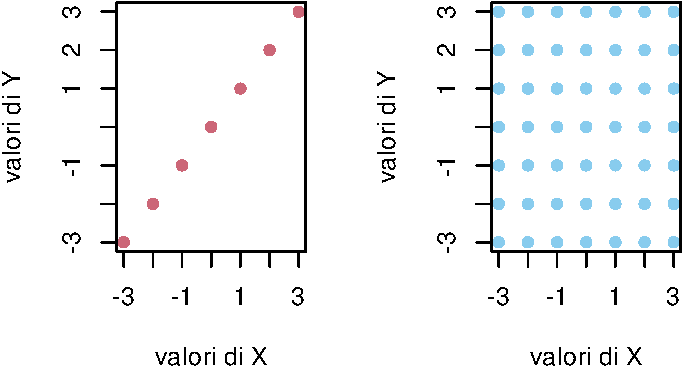
\includegraphics[keepaspectratio]{04-VA_indicatori_files/figure-pdf/unnamed-chunk-11-1.pdf}}

}

\caption{La densità di \((X,Y)\) assumendo \(X=Y\) è concentrata sulla
diagonale (a sinistra), mentre assumendo che siano indipendenti è
diffusa su tutte le possibili coppie (a destra)}

\end{figure}%

Questo motiva l'introduzione di un indicatore ``congiunto'' tra le
possibil coppie di componenti, noto come \emph{covarianza} (in inglese
\emph{covariance}), così definito.

Date due variabili aleatorie reali \(X\), \(Y\), si definisce la
covarianza tra esse come la quantità reale
\[ \Cov{X,Y} = \E {(X-\E{X})(Y-\E{Y})}.\]

A volte si indica anche \(\Cov{X,Y} = K_{XY}\). La covarianza è una
estensione della varianza, come mostra la seguente proposizione. Inoltre
è una funzione \emph{bilineare} (ossia separatamente lineare) dei suoi
due argomenti \(X\), \(Y\).

Date variabili aleatorie reali \(X\), \(Y\), \(Z\) e una costante
\(a>0\), valgono le seguenti proprietà: 1. \(\Cov{X, X} = \Var{X}\) 2.
(simmetria) \(\Cov{X,Y} = \Cov{Y,X}\) 3. (bilinearità)
\(\Cov{X+Z, Y} = \Cov{X,Y} + \Cov{Z, Y}\) e similmente
\(\Cov{X, Y+Z} = \Cov{X,Y} + \Cov{X,Z}\). Inoltre
\(\Cov{aX, Y} = a \Cov{X,Y} = \Cov{X, aY}\). 4. (varianza della somma)
\(\Var{X+Y} = \Var{X}+ \Var{Y}+ 2\Cov{X,Y}\). 5. (formula alternativa)
\(\Cov{X,Y} = \E{XY} - \E{X}\E{Y}\).

\begin{proof}
La dimostrazione è piuttosto immediata (in particolare la formula
alternativa segue analogamente al caso della varianza).
\end{proof}

Una proprietà importantissima della covarianza è la seguente.

Se due variabili reali \(X\), \(Y\) sono indipendenti (rispetto ad una
informazione \(I\)), allora sono \emph{non correlate}, ossia
\[ \Cov{X,Y }  = 0.\] In particolare, \[\Var{X+Y} = \Var{X} +\Var{Y}.\]

\begin{proof}
Questo fatto segue dalla formula alternativa per la covarianza
\[ \Cov{X,Y} = \E{XY} - \E{X}\E{Y}\] e la proposizione
\textbf{?@sec-valor\_medio\_indipendenti}, che garantisce
\[ \E{XY} = \E{X}\E{Y}.\]
\end{proof}

Riprendendo con l'esempio sopra, notiamo che, se l'informazione nota
\(I\) garantisce che \(X=Y\), allora la covarianza tra \(X\) e \(Y\)
coincide con la varianza (che era \(2\)). Se invece l'informazione \(I\)
implica che \(X\) e \(Y\) siano indipendenti, la covarianza sarà nulla.
Ecco quindi che tramite la covarianza possiamo indicare una differenza
tra le due leggi congiunte

Più in generale, il \emph{segno} della covarianza è una quantità
piuttosto indicativa. Si dice che \(X\) e \(Y\) sono
\emph{positivamente} correlate se \(\Cov{X,Y} >0\), mentre
\emph{negativamente} correlate se \(\Cov{X,Y}<0\).

Si considerino due variabili \(X \in \cur{0,1}\), indicatrice
dell'evento \(A\), \(Y \in \cur{0,1}\) indicatrice dell'evento \(B\).
Allora, usando il semplice fatto che il valor medio di una indicatrice è
la probabilità dell'evento che indica, e che \(XY \in \cur{0,1}\) è
indicatrice di ``\(A\) e \(B\)'', segue che
\[ \Cov{X,Y} = \E{XY} - \E{X}\E{Y} = P(A \text{ e  } B) - P(A) P(B).\]
In particolare, avremo che \(X\) e \(Y\) sono positivamente correlate se
e solo se
\[ P(A \text{ e  } B) - P(A) P(B) >0, \quad \text{ossia} \quad \frac{ P(A \text{ e } B) }{P(A) P(B) } >1,\]
Notiamo che sono negativamente correate se e solo se il rapporto di
sopra è minore di \(1\), mentre sono non correlate se e solo se il
rapporto vale \(1\) (e quindi sono indipendenti).

L'esempio sopra è molto speciale: in generale \emph{non} è possibile
dedurre che \(X\), \(Y\) siano indipendenti dal fatto che
\(\Cov{X,Y}=0\).

Come intepretare il segno della covarianza nel caso di variabili
generali? Vedremo una spiegazione precisa trattando la regressione
lineare nella Sezione Sezione~\ref{sec-regressione}. Non è una grave
approssimazione tuttavia rifarsi all'esempio precedente. In altre
parole, \(X\) e \(Y\) sono positivamente correlate se, sapendo che
\(X>\E{X}\) allora è più probabile che sia anche \(Y>\E{Y}\) (e
similmente, sapendo \(X\le \E{X}\), è più probabile che sia
\(Y \le \E{Y}\)). Graficamente, stiamo dicendo che la densità congiunta
tra \((X,Y)\) è circa concentrata nel primo e terzo quadrante
cartesiano, avendo posto l'origine nel vettore dei valor medi.
Viceversa, la correlazione negativa indica che la densità congiunta è
concentrata nel secondo e quarto quadrante. Torneremo su questo fatto
trattando le variabili gaussiane e la regressione lineare.

Avendo definito la covarianza tra coppie di variabili aleatorie reali,
dato un vettore aleatorio \(X \in \R^d\) possiamo introdurre una matrice
quadrata che collezioni tutte le covarianze tra le possibli coppie di
componenti (e sulla diagonale le varianze).

Dato un vettore aleatorio \(X = (X_1, \ldots, X_d) \in \R^d\), si
definisce la matrice delle covarianze di \(X\) la matrice di numeri
reali \(\Sigma_X \in \R^{d\times d}\) data da
\[ (\Sigma_X)_{i,j} = \Cov{X_i, X_j} = \E{X_iX_j} - \E{X_i}\E{X_j} \quad \text{per $i$, $j \in \cur{1, \ldots, d}$.}\]

Vi sono molteplici notazioni alternative per la matrice delle
covarianze, ad esempio \(\Var{X}\), \(K_{XX}\) o \(Q_X\). La matrice
delle covarianze è simmetrica \(\Sigma_X = \Sigma_X^T\), dove \(T\)
indica l'operazione di trasposizione e analogamente al vettore delle
medie, ha delle buone proprietà di trasformazione tramite funzioni
lineari affini.

Sia \(X \in \R^d\) una variabile aleatoria e sia
\[ Y = AX+b \quad \text{ossia} \quad Y_i = \sum_{j=1}^d A_{ij} X_j + b_i,\]
dove \(A \in \R^{k \times d}\) è una matrice e \(b \in \R^k\) è un
vettore (costanti rispetto all'informazione nota \(I\)), vale
\[ \Sigma_{AX+b} = A \Sigma_X A^T.\] In particolare, se \(k=1\) e
\(A = v^T\), con \(v \in \R^{d}\), si ottiene che
\[  \Var{v \cdot X}= \Sigma_{v\cdot X} = v^T \Sigma_X v,\] ossia
\(\Sigma_X\) è (semi-)definita positiva.

\begin{proof}
Si calcola, usando la bilinearità della covarianza,
\[  \begin{split} \Cov{Y_i, Y_{i'} } & =  \Cov{  \sum_{j=1}^d A_{ij} X_j,   \sum_{j'=1}^d A_{i'j'} X_{j'}}\\
&  = \sum_{j,j' = 1}^d A_{ij}\Cov{X_j, X_{j'}} A_{i' j'}
\end{split}\] che coincide con \((A \Sigma_X A^T)_{ii'}\).
\end{proof}

Da questo seguono due conseguenze importanti. Nel caso \(d=2\),
scrivendo \((X,Y)\) per la variabile congiunta di due variabili reali
\(X\), \(Y\), la matrice delle covarianze è esplicitamente
\[ \Sigma_{(X,Y)} = \bra{ \begin{array}{cc}\Var{X} & \Cov{X,Y}\\ 
\Cov{X,Y} & \Var{Y} \end{array}}.\]

Essendo semidefinita positiva, il suo determinante è positivo (o nullo):
\[\det(\Sigma_{(X,Y)}) = \Var{X}\Var{Y} - (\Cov{X,Y})^2 \ge 0,\] ossia,
dopo alcune operazioni elementari, si ha che
\[ \rho_{XY} := \frac{ \Cov{X,Y}}{\sigma_X \sigma_Y} \in [-1,1].\] Tale
quantitàla quantità, detta \emph{coefficiente di correlazione} (o indice
di correlazione di Pearson), è una covarianza normalizzata alle due
deviazione standard (di \(X\) e di \(Y\)) e ha il vantaggio di indicare
sia il segno della covarianza (e quindi positiva o negativa
correlazione), sia di \emph{quantificare} una eventuale dipendenza
\emph{lineare} tra \(X\) e \(Y\). Infatti si potrebbe dimostrare che
\(\rho_{XY} \in \cur{-1,1}\) se e solo se esistono costanti
\(a, b \in \R\) tale che \(Y = aX+b\).

La seconda conseguenza è una applicazione del teorema spettrale per
matrici reali simmetriche (caso speciale delle hermitiane complesse),
che permette di decomporre \[ \Sigma_X = U^T D U,\] per una opportuna
matrice ortogonale \(U \in \R^{d\times d}\), ossia tale che
\(U^T U = Id\) e una matrice diagonale \(D\). La matrice diagonale
contiene tutti gli autovalori di \(\Sigma_X\) (in particolare sono
positivi o nulli). Se consideriamo la trasformazione \(UX\), che
corrisponde ad cambio di coordinate dalla base canonica di \(\R^d\) alla
base ortonormale data dalle colonne di \(U\), la covarianza si trasforma
di conseguenza come \[ \Sigma_{UX} = U \Sigma_X U^T = D,\] ossia le
componenti di \(UX\) sono a due a due non correlate. Questo può essere
visto come un primo passo per una ``standardizzazione'' di un vettore
aleatorio. Se \(D\) è invertibile (ossia gli autovalori sono tutti
positiv), si può in effetti definire
\(\hat{X} = \sqrt{D}^{-1} U(X-\E{X})\), dove \(\sqrt{D}\) è la matrice
diagonale con entrate date dalla radice quadrata di quelle di \(D\).
Usando le proprietà del vettore delle medie e della varianza, si ha
\[ \E{\hat{X} } = 0 \in \R^d \quad \text{e} \quad \Sigma_{ \hat{X} } = Id.\]

\subsection{Esercizi}\label{esercizi-21}

Sia \(X\) uniforme continua su \([0, 2 \pi]\) e siano \(U = \cos(X)\),
\(V = \sin(X)\). Calcolare \(\Cov(U,V)\).

Sia \(X\), una variabile esponenziale di parametro \(1\) e sia
\(Y = X^2\) Dire se \(X\), \(Y\) sono positivamente correlate.

\section{Momenti}\label{sec-mgf}

Supponiamo di dover calcolare il valor medio di una funzione composta
\(g(X)\), dove \(X \in \R\) è una variabile aleatoria e \(g:\R \to \R\)
è una funzione regolare. Una possibilità potrebbe essere di approssimare
\(g\) tramite un polinomio (possiamo pensare ad esempio allo sviluppo di
Taylor in un punto):
\[ g(x) \sim a_0 + a_1 x + a_2 x^2 + \ldots + a_k x^k\] dove
\(a_i \in \R\) sono costanti, e poi sfruttare la linearità del valor
medio per approssimare
\[ \E{g(X)} \sim a_0 + a_1 \E{X} + a_2 \E{X^2}+ \ldots + a_k \E{X^k}.\]
Certamente, bisogna fare attenzione al senso in cui l'approssimazione
vale. Il problema è decomposto in due sotto-problemi: 1. determinare un
polinomio approssimante per \(g\) (questo problema è del tutto analitico
e non riguarda \(X\)) 2. calcolare i valor medi \(\E{X}\), \(\E{X^2}\),
\ldots, \(\E{X^k}\), fino al grado massimo \(k\) richiesto dal polinomio
ottenuto al punto sopra.

Il vantaggio è evidente soprattutto se è richiesto di calcolare il valor
medio per più di una funzione \(g\), perché non serve ripetere il punto
\(2\) (supponendo che il grado massimo \(k\) non cambi). Per questa ma
anche altre ragioni, i valori \(\E{X}\), \(\E{X^2}\), \ldots,
\(\E{X^k}\) sono oggetto di studio particolare nel calcolo delle
probabilità e vengono detti \textbf{momenti} di una variabile aleatoria
\(X\).

Sia \(X \in \R\) una variabile aleatoria. Per ogni \(k \in \N\), si dice
\textbf{momento di ordine \(k\)} (o momento \(k\)-esimo) di \(X\) la
quantità \[\E {X^k},\] se è ben definita (ricordiamo che si richiede che
la serie o l'integrale che definisce \(\E{X^k}\) debba convergere).

Notiamo come al solito che il valor medio dipende comunque
dall'informazione \(I\) che si ritiene nota (ma evitiamo qui di
esplicitare per semplicità di scrittura).

Esplicitamente, se \(X\) ha densità (discreta o continua) vale
\[ \E{X^k} = \begin{cases} \sum_{x \in \R} x^k P(X=x) & \text{se $X$ ha densità discreta,}\\
\int_{x \in \R} x^k p(X=x)d x & \text{se $X$ ha densità continua.}
\end{cases}\]

In particolare, la legge di \(X\) determina unicamente i momenti di ogni
ordine (se esistono).

\begin{remark}
La formula alternativa per la varianza di una variabile aleatoria
\(X \in \R\), Proposizione \textbf{?@prp-varianza-alternativa}, afferma
che la varianza è scrivibile come combinazione del momento secondo e dal
momento primo. Essa può essere anche equivalentemente riscritta come
\[ \E{X^2} = \Var{X} + (\E{X})^2,\] fornendo un modo per calcolare il
momento secondo (nota la varianza e il momento primo).
\end{remark}

Data una variabile \(X\), per descrivere la densità in realtà risultano
più significativi i momenti della variabile standardizzata
\[ X'  = (X-\E{X})/\sigma_X.\] In particolare, il suo momento terzo è
detto \textbf{skewness} di \(X\) (e indica eventuale asimmetria della
densità rispetto alla media) mentre il momento quarto è detto
\textbf{kurtosi}.

Per agevolare il calcolo dei momenti, si introduce una funzione
ausiliaria, detta funzione generatrice dei momenti. Il vantaggio è che
riduce il problema dell'integrazione ad un solo integrale (dipendente da
un parametro), mentre i momenti si ricavano effettuando derivate
(tipicamente più semplici da calcolare).

Data \(X \in \R\) una variabile aleatoria reale, si definisce la sua
\textbf{funzione generatrice dei momenti} (in inglese \emph{moment
generating function}, \textbf{MGF}) la funzione
\(\operatorname{MGF}_X:  \R \to [0, \infty]\), che associa
\[ t \mapsto \operatorname{MGF}_X(t) = \E{ e^{tX}}.\]

Per ciascun \(t \in \R\), il valor medio si calcola quindi come
\[ \operatorname{MGF}_X(t) = \E{e^{tX}} = \begin{cases} \sum_{x \in \R} e^{tx} P(X=x) & \text{se $X$ ha densità discreta,}\\
\int_{x \in \R} e^{tx} p(X=x)dx & \text{se $X$ ha densità continua.}
\end{cases}
(\#eq:integrale-mgf)\]

Se per qualche \(t \in \R\) l'integrale o la serie che definiscono il
valor medio di \(\E{e^{tX}}\) non convergono, si pone
\(\operatorname{MGF}_X(t) =\infty\). In effetti, può accadere che la
funzione generatrice dei momenti valga \(\infty\) in molti valori
\(t \in \R\), tuttavia almeno per \(t =0\) è finita. Infatti:
\[ \operatorname{MGF}_X(0) = \E{ e^{0 \cdot X}} = \E{1} = 1.\] Il
vantaggio di calcolare la \(\operatorname{MGF}_X\) rispetto a tutti i
momenti è che spesso l'integrale (o la serie) pur dipendendo dal
parametro \(t\), si può calcolare con la stessa tecnica per tutti i
parametri (mentre spesso integrare o sommare i polinomi \(x^k\) richiede
tecniche particolari, come integrazioni per parti).

\begin{remark}
Per chi è familiare con il concetto di \emph{trasformata di Laplace} di
una funzione, si può riconoscere nell'integrale
\textbf{?@eq-integrale-mgf} appunto la trasformata di Laplace della
funzione densità continua \(x \mapsto p(X=x)\). Pertanto, se la funzione
è tra quelle la cui trasformata di Laplace è nota, si può evitarne il
calcolo.
\end{remark}

Sia \(X\in \R\) con densità continua esponenziale di parametro
\(\lambda>0\). Per calcolare la \(\operatorname{MGF}_X(t)\), basta
integrare
\[ \int_0^\infty e^{tx} e^{-\lambda x} \lambda dx = \begin{cases} \frac{\lambda}{\lambda-t} & \text{se $t<\lambda$,}\\
\infty & \text{altrimenti.}\end{cases}\] Notiamo in particolare che per
infiniti valori la funzione generatrice dei momenti è infinita.

Le seguenti proprietà elementari si mostrano con poco sforzo partendo
dalle proprietà dell'esponenziale e del valor medio.

Siano \(X\), \(Y \in \R\) variabili aleatorie e \(a\), \(b\in \R\)
costanti (rispetto all'informazione nota \(I\)). Allora 1.
\(\operatorname{MGF}_{aX+b}(t)= e^{tb} \operatorname{MGF}_{X}(at)\) 2.
Se \(X\), \(Y\) sono indipendenti, allora
\(\operatorname{MGF}_{X+Y}(t) = \operatorname{MGF}_{X}(t)\operatorname{MGF}_{Y}(t)\).

\begin{proof}
Per la prima,
\[ \operatorname{MGF}_{aX+b}(t)= \E{e^{t(aX+b)}} = \E{e^{tb} e^{(ta)X}} = e^{tb} \operatorname{MGF}_{X}(at).\]
Per la seconda, basta ricordare che \(e^{t(X+Y)} = e^{tX}e^{tY}\) e che
le variabili \(e^{tX}\), \(e^{tY}\) sono indipendenti (perché ciascuna
ottenuta tramite composizione \emph{separata} di variabili
indipendenti). Quindi, \[\E{e^{tX}e^{tY}} = \E{e^{tX}}\E{e^{tY}}.\]
\end{proof}

Il seguente teorema definisce il legame tra \(\operatorname{MGF}_X\) e i
momenti di \(X\).

Sia \(X \in \R\) tale che \(\operatorname{MGF}_X(t)<\infty\) per ogni
\(t \in (-\varepsilon, \varepsilon)\), per qualche \(\varepsilon>0\).
Allora, per ogni \(k \in \N\), \(X\) ha momento di ordine \(k\) ben
definito e vale
\[ \frac{d^k}{d^k t} \operatorname{MGF}_X(0) = \E{X^k}.\]

Per calcolare il momento di ordine \(k\) è quindi sufficiente derivare
\(k\) volte la \(\operatorname{MGF}_X(t)\) e successivamente porre
\(t=0\).

\begin{proof}
Non diamo qui una dimostrazione completamente rigorosa, ma ci limitiamo
a mostrare perché la formula per il momento di ordine \(k\) dovrebbe
essere appunto quella proposta.

Scrivendo la serie di Taylor per la funzione esponenziale, si trova
\[ e^{tx} = \sum_{k=0}^\infty \frac{(tx)^k}{k!} = \sum_{k=0}^\infty x^k \frac{t^k}{k!} ,\]
Componendo con \(X\) la funzione \(e^{tx}\), vale allora
\[ e^{tX} = \sum_{k=0}^\infty X^k \frac{t^k}{k!}.\] Passando al valor
medio, e usando la linearità (anche se si tratta di una serie invece di
una somma finita), troviamo che
\[ \operatorname{MGF}_X(t) = \E{e^{tX}}= \sum_{k=0}^\infty \E{X^k} \frac{t^k}{k!}.\]
Confrontando il membro a destra con però la serie di Taylor (centrata in
\(0\)) per la funzione generatrice dei momenti, si trova
t\[  \sum_{k=0}^\infty \frac{d^k}{d^k t} \operatorname{MGF}_X(0) \frac{t^k}{k!} =  \sum_{k=0}^\infty \E{X^k} \frac{t^k}{k!},\]
da cui la tesi.
\end{proof}

\begin{remark}
Si può estendere il concetto di momento a variabili vettoriali
\(X \in \R^d\), considerando prodotti delle marginali. Ad esempio, il
momento primo corrisponde al vettore dei valor medi, il vettore secondo
alla collezione dei valor medi
\[ \E{X_i X_j} \quad \text{per $i, j \in \cur{1, \ldots, d}$ (anche $i=j$)}\]
e il momento terzo invece
\[ \E{X_i X_j X_j} \quad \text{per $i, j,k \in \cur{1, \ldots, d}$.}\]
In questo caso, la funzione generatrice dei momenti diventa una funzione
di \(d\) variabili \((t_1, t_2, \ldots, t_d)\) (oppure di una singola
variabile vettoriale \(t\in \R^d\)), ed è definita come
\[ \operatorname{MGF}_{X}(t) = \E{\exp \bra{ \sum_{i=1}^d t_i X_i}}.\]
Il legame tra questa funzione e i momenti è dato dalle derivate parziali
valutate in \(t=0\).
\end{remark}

\subsection{Esercizi}\label{esercizi-22}

Calcolare la skewness e la curtosi di una variabile continua con densità
esponenziale di parametro \(\lambda\). Plottare tali valori come
funzione di \(\lambda>0\).

Calcolare la \(\operatorname{MGF}_X\) per \(X\) uniforme continua su
\([a,b]\) e determinarne skweness e curtosi.

Calcolare \(\operatorname{MGF}_X\) di una variabile \(X\) avente densità
discreta binomiale di parametri \((n,p)\) \emph{(suggerimento: scrivere
\(X\) come somma \(n\) variabili Bernoulli indipendenti)}.

\section{Funzione caratteristica}\label{sec-caratteristica}

Ritornando alla motivazione per l'introduzione dei momenti \(\E{X^k}\)
di una variabile aleatoria \(X\in \R\), ossia il calcolo approssimato di
\(\E{g(X)}\) possiamo anche sfruttare approssimazioni di \(g(x)\) in una
``base di funzioni'' diversa dai polinomi. Una possibilità è data dalla
teoria della \emph{trasformata di Fourier}\footnote{si veda l'Appendice
  \textbf{?@sec-app\_fourier} per richiami sull'argomento e le notazioni},
per cui ogni \(g\) sufficientemente regolare si può scrivere come
trasformata inversa, tramite la formula di inversione
\[ g(x) =  \int_{-\infty}^\infty \hat{g}(\xi) e^{2 \pi i \xi x} d \xi,\]
dove \(\hat{g}(\xi)\) è la trasformata (diretta) di Fourier,
\[ \hat{g}(\xi)= \int_{-\infty}^\infty g(x) e^{-2 \pi i \xi x} d x.\]
Posta \(\omega = 2 \pi \xi\) la frequenza angolare\footnote{Si tratta
  solo un cambio di variabile per non avere i coefficienti \(2 \pi\)
  nelle formule d'ora in avanti. A volte si indica anche con \(t\)
  invece di \(\omega\), per non confondersi con gli elementi
  dell'insieme ``universo'' \(\Omega\) di Kolmogorov, con cui in questo
  caso non ha nulla a che fare. Qui usiamo la notazione \(\omega\) per
  ricordare che rappresenta una frequenza angolare e non c'è il rischio
  di confusione perché non ci riferiamo mai agli assiomi di Kolmogorov}
possiamo quindi approssimare l'integrale sopra con una certa somma
finita, per opportuni coefficienti \(a_\omega\) (non aleatori)
\[ g(x) \sim \sum_{\omega} a_\omega e^{i \omega x}\] e quindi,
componendo con \(X\) e passando al valor medio, troviamo
\[\E{g(X)} \sim \sum_{\omega} a_\omega \E{e^{i \omega X}}.\] In analogia
con quanto visto per i momenti, possiamo quindi ridurre il problema
(almeno quello che riguarda la variabile \(X\)) al calcolo dei numeri
complessi
\[ \E{e^{i \omega X}} = \E{\cos(\omega X)}+ i \E{\sin(\omega X)},\] al
variare di \(\omega \in \R\). Notiamo che la notazione esponenziale
evidenzia un'analogia con la \(\MGF_X\) (stiamo formalmente ponendo
\(t = i \omega\)). Definiamo allora la seguente funzione.

Data una variabile aleatoria \(X \in \R\), si definisce la sua
\textbf{funzione caratteristica} \(\varphi_X: \R \to \mathbb{C}\),
\[ \omega \mapsto \varphi_X(\omega) = \E{e^{i \omega X}}.\]

Diversamente dalla funzione generatrice dei momenti, si può mostrare che
\(\varphi_X(\omega)\) è sempre un numero complesso ben definito, che si
calcola tramite serie o integrale (se la densità di \(X\) è nota)
\[ \varphi_X(\omega) = \E{e^{i \omega X}} = \begin{cases} \sum_{x \in \R} e^{i\omega x} P(X=x) & \text{se $X$ ha densità discreta,}\\
\int_{x \in \R} e^{i \omega x} p(X=x)dx & \text{se $X$ ha densità continua.}
\end{cases}
(\#eq:integrale-caratteristica)\]

L'integrale sopra, a meno di cambiare il segno a \(\omega\), è la
proprio \emph{trasformata di Fourier} della densità \(p(X=x)\), ossia
\[ \varphi_X(\omega) = \widehat{p(X=\cdot)} (-\omega).\] Questa
identificazione permette di sfruttare le formule note per la trasformata
di Fourier di molte funzioni comuni.

La seguente proposizione si mostra in modo analogo a quanto fatto per la
funzione generatrice dei momenti (tenendo conto tuttavia che abbiamo a
che fare con quantità complesse, quindi il prodotto è inteso tra numeri
complessi).

Siano \(X\), \(Y \in \R\) variabili aleatorie e \(a\), \(b\in \R\)
costanti (rispetto all'informazione nota \(I\)). Allora 1.
\(\varphi_{aX+b}(\omega)= e^{i \omega b} \varphi_{X}(a\omega)\) 2. Se
\(X\), \(Y\) sono indipendenti, allora
\(\varphi_{X+Y}(\omega) = \varphi_{X}(\omega)\varphi_{Y}(\omega)\).

Come per la funzione generatrice dei momenti, se si può derivare la
funzione caratteristica in \(\omega =0\), si ottengono i momenti (a meno
di potenze dell'unità immaginaria stavolta).

Sia \(X \in \R\) tale che abbia momento di ordine \(k\) finito. Allora
vale \[ \frac{d^k}{d^k \omega} \varphi_X(0) = i^k \E{X^k}.\]

La giustificazione (non rigorosa) segue ancora dalla formula di Taylor
per l'esponenziale (di parametro complesso, stavolta):
\[ e^{ i \omega x} = \sum_{k=0}^\infty \frac{(i \omega x)^k}{k!} = \sum_{k=0}^\infty x^k \frac{(i\omega)^k}{k!} 
 ,\] e ripetendo gli stessi passaggi fatti per la funzione generatrice
dei momenti.

Una proprietà estremamente importante della funzione caratteristica è
che essa \emph{identifica} la legge di \(X\). Questo non stupisce almeno
nel caso di densità continue, perché la formula di inversione della
trasformata di Fourier permette di ricavare \(p\), ma il seguente
risultato -- che non dimostriamo -- è generale.

\protect\phantomsection\label{iniettivita-fourier}
Siano \(X\), \(Y \in \R\) variabili aleatorie. Se
\(\varphi_X(\omega)= \varphi_Y(\omega)\) per ogni \(\omega \in \R\),
allora \(X\) e \(Y\) hanno la stessa legge, ossia
\[ P( X \in U)  = P( Y \in U)\] per ogni \(U \subseteq  \R\) (ad esempio
\(U = [a,b]\) intervallo). In particolare, se \(X\) ha densità (discreta
o continua) allora anche \(Y\) ha densità (uguale a quella di \(X\)).

\begin{remark}
Si può estendere il concetto di trasformata di Fourier e quindi di
funzione caratteristica a variabili vettoriali \(X \in \R^d\). In questo
caso, essa diventa una funzione di \(d\) variabili
\((\omega_1, \omega_2, \ldots, \omega_d)\) (oppure di una singola
variabile vettoriale \(\omega \in \R^d\)), ed è definita come
\[ \varphi_{X}(\omega) = \E{e^{i t\cdot \omega}} = \E{ \exp \bra{ \sum_{i=1}^d\omega_i X_i}}.\]
Si può mostrare, usando la definizione sopra, che vale
\[  \varphi_{AX+b} (\omega) = e^{i b \cdot \omega} \varphi_X(A^T \omega)\]
per qualsiasi matrice \(A \in \R^{k \times d}\) e vettore \(b \in \R^k\)
(costanti rispetto all'informazione nota \(I\)). Inoltre, il Teorema
\textbf{?@thm-iniettivita-fourier} si estende anche al caso vettoriale:
se due variabili \(X\), \(Y \in \R^d\) hanno la medesima funzione
caratteristica (valutata in ogni \(\omega\in \R^d\)), allora hanno la
stessa legge (e quindi densità, se si sa che una delle due ha densità).
\end{remark}

\subsection{Esercizi}\label{esercizi-23}

Calcolare la funzione caratteristica di una variabile con densità
discreta binomiale di parametri \((n,p)\). Derivare l'espressione
trovata per calcolare media e varianza.

La funzione caratteristica di una variabile aleatoria reale \(X\) è data
dall'espressione
\[ \varphi_X(\omega) = \frac 1 2 + \frac 1 3 e^{i \omega} + \frac 1 6 e^{- i \omega}\]
Calcolare media e deviazione standard di \(X\).

\section{Entropia}\label{sec-entropia}

Concludiamo questo capitolo con un indicatore leggermente diverso, ma
estremamente importante in molti ambiti (dalla fisica alla teoria
dell'informazione): si tratta dell'\textbf{entropia} di una variabile
aleatoria \(X\), o più precisamente della densità (discreta o continua)
di \(X\) rispetto ad una informazione nota \(I\).

Prima di darne la definizione formale, premettiamo che lo scopo è di
introdurre una misura del grado di ``ignoranza'' del robot riguardo a
quale delle alternative associate alla variabile \(X\) sia in effetti
quella vera. Maggiore sarà tale quantità, detta appunto entropia,
maggiore sarà l'ignoranza del robot. Spesso si preferisce usare il
termine ``assenza di informazione'' piuttosto che ``ignoranza'',
pertanto ragionando nel verso opposto avremo che, minore sarà
l'entropia, maggiore sarà invece la ``quantità di informazione'' che il
robot dispone riguardo alle alternative associate ad \(X\).

È chiaro che vi saranno diverse quantità che rappresentato l'intuizione
sopra descritta: si può tuttavia argomentare che l'unica quantità che
soddisfa determinate ``regole di calcolo'' naturali (che tuttavia qui
non vedremo) è data dalla seguente espressione:
\[ H(X) = \begin{cases} -\sum_{x \in E} P(X= x) \log( P(X=x)) & \text{ se $X \in E$ ha densità discreta,}\\
 -\int_{\R^d} p(X= x) \log( p(X=x)) d x & \text{ se $X\in \R^d$ ha densità continua.}\end{cases}\]

Come al solito, non evidenziamo l'informazione nota \(I\) rispetto alla
quale è sempre intesa la densità, e quindi l'entropia di \(X\). La
scelta di base del logaritmo, specie nel caso discreto, dipende dai vari
ambiti (noi useremo la base naturale, in altri casi è preferibile la
base \(2\)).

Per \(z \in [0,1]\), la funzione \(-z \log (z)\) è sempre positiva (e
nulla solo se \(z =0\) oppure \(z=1\)). Ne segue che, nel caso discreto,
\(H(X) \ge 0\). In particolare, se la densità discreta assume solo
valore \(0\) oppure \(1\) (in altre parole \(X\) è costante rispetto
all'informazione \(I\)), l'entropia \(H(X)\) è minima -- che ben
rappresenta il fatto che l'ignoranza sia minima, in quanto il robot
dispone una conoscenza certa della \(X\).

Nel caso continuo invece l'entropia può anche essere negativa (perché la
densità continua può essere maggiore di \(1\)).

\begin{Shaded}
\begin{Highlighting}[]
\NormalTok{deltaz}\OtherTok{=} \FloatTok{0.001}
\NormalTok{z}\OtherTok{=}\FunctionTok{seq}\NormalTok{(}\DecValTok{0}\NormalTok{,}\DecValTok{2}\NormalTok{, }\AttributeTok{by=}\NormalTok{deltaz)}


\FunctionTok{plot}\NormalTok{(z, }\SpecialCharTok{{-}}\NormalTok{z}\SpecialCharTok{*}\FunctionTok{log}\NormalTok{(z),  }\AttributeTok{ylab=}\StringTok{\textquotesingle{}{-}z log(z)\textquotesingle{}}\NormalTok{, }\AttributeTok{type=}\StringTok{\textquotesingle{}l\textquotesingle{}}\NormalTok{, }\AttributeTok{col=}\NormalTok{miei\_colori[}\DecValTok{2}\NormalTok{], }\AttributeTok{lwd=}\DecValTok{3}\NormalTok{)}
\FunctionTok{lines}\NormalTok{(z, }\DecValTok{0}\SpecialCharTok{*}\NormalTok{z, }\AttributeTok{type=}\StringTok{\textquotesingle{}l\textquotesingle{}}\NormalTok{, }\AttributeTok{col=}\StringTok{\textquotesingle{}grey\textquotesingle{}}\NormalTok{)}
\FunctionTok{points}\NormalTok{(}\FunctionTok{c}\NormalTok{(}\DecValTok{0}\NormalTok{,}\DecValTok{1}\NormalTok{), }\FunctionTok{c}\NormalTok{(}\DecValTok{0}\NormalTok{,}\DecValTok{0}\NormalTok{), }\AttributeTok{col=}\NormalTok{miei\_colori[}\DecValTok{2}\NormalTok{], }\AttributeTok{pch=}\DecValTok{19}\NormalTok{)}
\end{Highlighting}
\end{Shaded}

\begin{figure}[H]

{\centering \pandocbounded{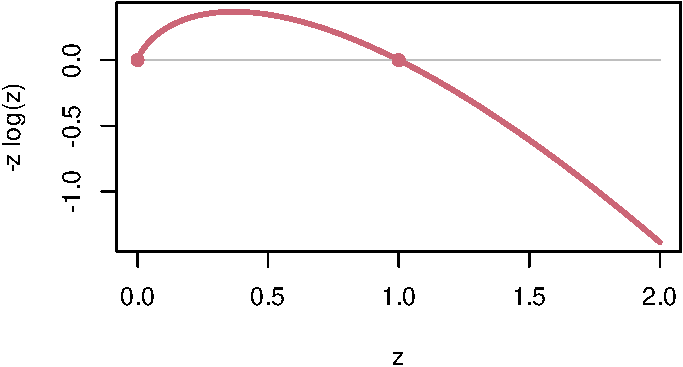
\includegraphics[keepaspectratio]{04-VA_indicatori_files/figure-pdf/unnamed-chunk-12-1.pdf}}

}

\caption{grafico della funzione \(-z\log(z)\).}

\end{figure}%

Vediamo come in alcuni esempi fondamentali l'entropia si adegua bene
all'idea di misura di ``assenza di informazione'' (o ignoranza del
robot).

Nel caso di \(X \in \cur{0,1}\) con legge Bernoulli di parametro
\(p \in [0,1]\), l'entropia è data da
\[ H(X) = -(1-p)\log(1-p) - p \log (p).\] Essa è detta anche entropia
binaria e indicata \(H(p)\). Possiamo visualizzare la quantità
graficamente, al variare di \(p\) in figura. Vediamo che è minima
(nulla) ai valori estremi \(p=0\), \(p=1\) (perché in tal caso il robot
conosce \(X\) che è costante \(0\) oppure \(1\)), mentre è massima nel
caso \(p=1/2\), ossia quando le due alternative hanno uguale
probabilità.

\begin{Shaded}
\begin{Highlighting}[]
\NormalTok{deltap}\OtherTok{=} \FloatTok{0.001}
\NormalTok{p}\OtherTok{=}\FunctionTok{seq}\NormalTok{(}\DecValTok{0}\NormalTok{,}\DecValTok{1}\NormalTok{,}\AttributeTok{by=}\NormalTok{deltap)}

\NormalTok{H\_p }\OtherTok{=} \SpecialCharTok{{-}}\NormalTok{(}\DecValTok{1}\SpecialCharTok{{-}}\NormalTok{p)}\SpecialCharTok{*}\FunctionTok{log}\NormalTok{(}\DecValTok{1}\SpecialCharTok{{-}}\NormalTok{p)}\SpecialCharTok{{-}}\NormalTok{p}\SpecialCharTok{*}\FunctionTok{log}\NormalTok{(p)}

\FunctionTok{plot}\NormalTok{(p, H\_p, }\AttributeTok{type=}\StringTok{\textquotesingle{}l\textquotesingle{}}\NormalTok{, }\AttributeTok{xlab=}\StringTok{\textquotesingle{}p\textquotesingle{}}\NormalTok{, }\AttributeTok{ylab=}\StringTok{\textquotesingle{}H(p)\textquotesingle{}}\NormalTok{, }\AttributeTok{lwd=}\DecValTok{3}\NormalTok{, }\AttributeTok{col=}\NormalTok{miei\_colori[}\DecValTok{2}\NormalTok{] )}
\end{Highlighting}
\end{Shaded}

\begin{figure}[H]

{\centering \pandocbounded{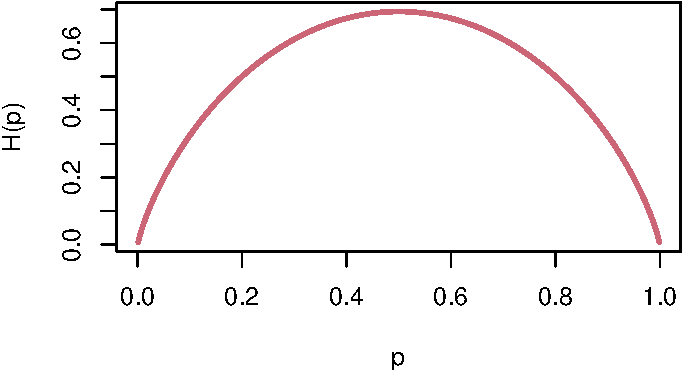
\includegraphics[keepaspectratio]{04-VA_indicatori_files/figure-pdf/unnamed-chunk-13-1.pdf}}

}

\caption{Entropia di una densità Bernoulli al variare del parametro
\(p\)}

\end{figure}%

Possiamo calcolare l'entropia di una variabile uniforme, sia nel caso
discreto (su \(n\) valori) che nel caso continuo (su un intervallo
\([a,b]\)). Nel primo caso (discreto) troviamo
\[ H( X \text{ uniforme su $n$ valori})  = -\sum_{i=1}^n \log\bra{ \frac 1 n } \frac 1 n = \log(n),\]
mentre nel secondo caso (continuo) troviamo
\[ H(X \text{ uniforme continua su $[a,b]$}) = - \int_a^b \log\bra{ \frac  1 {b-a}} \frac 1 {b-a} dx = \log(b-a).\]
Troviamo quindi che \(H(X)\) è in entrambi i casi data dal logaritmo
della ``ampiezza'' dei possibili valori. In particolare, più grande è
tale insieme, maggiore è l'entropia, in accordo con il fatto che il
robot è in tal caso più ignorante. Notiamo anche che se \(b-a<1\),
allora l'entropia diventa negativa (cosa possibile nel caso continuo, ma
non nel caso discreto).

Oltre ad essere una quantità utile di per sé, l'entropia ha un ruolo
importante nel determinare densità (discrete o continue) per variabili
aleatorie \(X\) qualora l'informazione fornita in un problema non sia
sufficiente a calcolarle direttamente. È possibile infatti introdurre un
\textbf{principio di massima entropia}, che estende il principio di
indifferenza di Laplace (quello secondo il quale date \(n\) alternative
indistinguibili, si deve assegnare densità uniforme discreta). Il
principio afferma che il robot, qualora non possa determinare unicamente
la densità di \(X\), ma abbia identificato un insieme \(\mathcal{D}\) di
possibili densità che rispettano l'informazione di cui egli dispone (di
solito l'informazione iniziale del problema), allora egli
\emph{sceglierà l'unica densità per cui \(H(X)\) sia massima tra quelle
in \(\mathcal{D}\)}. La ragione sottostante è che in questo modo
rappresenta il più efficacemente possibile il suo stato di
``ignoranza'', pur comunque ottenendo una certa densità in modo da
ottenere una possibile soluzione del problema.

Tale principio, estremamente generale, si concretizza poi in casi
speciali in cui determinate densità si possono mostrare essere di
\textbf{massima entropia} per determinati insiemi \(\mathcal{D}\). Il
fatto che una densità sia di massima entropia ne giustifica
ulteriormente l'uso nella pratica, magari già affermato per altre
ragioni.

Si può dimostrare che, al variare di tutte le densità discrete di
variabili aleatorie \(X\) su un insieme \(E\) finito contenente \(n\)
elementi (quindi \(X\) assume al più \(n\) valori), l'entropia \(H(X)\)
è massima se e solo se \(X\) è uniforme. Similmente fissato un
intervallo \([a,b]\), nel caso di variabili aleatorie \(X\) con densità
continua su un intervallo \((a,b)\) (ossia tali che \(P(a<X<b )=1\)), si
può mostrare che l'entropia \(H(X)\) è massima se e solo se \(X\) è
uniforme continua (più formalmente, in questo caso abbiamo che
\(\mathcal{D} = \cur{ \text{"densità continue $p(X=x)$ nulle fuori da $(a,b)$"}}\)).

Fissato \(m>0\), si può considerare l'insieme \(\mathcal{D}\) delle
densità continue \(p(X=x)\) nulle fuori da \([0, \infty)\) e di valor
medio fissato \[ \int _0^\infty  x p(X=x) d x = m.\] Questa classe
interviene quando l'informazione di cui il robot dispone è che una
variabile aleatoria \(X\) è continua, positiva ed è noto il suo valor
medio \(m\). Sulla base di questa informazione, l'entropia è massima nel
caso di una densità continua esponenziale di parametro
\(\lambda = m^{-1}\) (in modo che il valor medio sia appunto \(m\)).

L'analogo discreto dell'esempio sopra consiste nel sapere che una
variabile aleatoria a valori in \(\N\) ha valor medio \(m\). L'insieme
\(\mathcal{D}\) consiste delle densità discrete \(P(X=k)\), per
\(X \in \N\) e di valor medio fissato
\[ \sum_{k =0}^\infty k P(X=k)  = m.\] In questo caso, l'entropia è
massima per una variabile con densità discreta \textbf{geometrica},
ossia tale che \(P(X=k) \propto (1-p)^k\)\$, per un parametro
\(p \in [0,1]\) (ovviamente si può anche porre direttamente \(q=1-p\),
ma tradizionalmente si parametrizza in questo modo). Si può calcolare
esplicitamente \[ P(X=k) = p (1-p)^k\] e inoltre si calcola (ad esempio
a partire dalla \(\operatorname{MGF}_X\) che si calcola esplicitamente),
\[ \E{X} = \frac{1-p}{p},\] da cui \(p = 1/(m+1)\) e quindi si può anche
scrivere \[ P(X=k) = \frac{1}{m+1} \bra{ \frac m {m+1}}^k.\]

\begin{remark}
L'entropia qui introdotta ha applicazioni in vari ambiti applicati, e
per prima nella teoria dell'informazione, ma anche in fisica (anche se
intepretata in modo leggermente diverso). Una applicazione importante in
statistica e apprendimento automatico riguarda anche l'uso di
\emph{distanze} tra densità di probabilità basate sull'entropia, come la
\textbf{divergenza di Kullback-Leibler} o la sua variante simmetrica, la
\textbf{divergenza di Jensen-Shannon}, che tuttavia non tratteremo.
\end{remark}

\subsection{Esercizi}\label{esercizi-24}

Calcolare l'entropia di una variabile con densità continua esponenziale
di parametro \(\lambda\), e rappresentarla graficamente al variare del
parametro.

In molti casi si può intepretare l'entropia come una ulteriore misura di
``dispersione'' della densità di \(X\), simile alla varianza. Trovare
però degli esempi di densità (ad esempio discrete) la cui entropia sia
molto bassa (ossia \(<1/n\)) ma la varianza sia molto grande (diciamo
\(>n\)). \emph{(Suggerimento: l'entropia nel caso discreto non dipende
dagli specifici valori che la variabile può assumere, ma solo dalla sua
densità)}

\section{Problemi}\label{problemi-2}

Usando la serie geometrica \(\sum_{k=0}^\infty x^k = 1/(1-x)\), per
\(|x|<1\), calcolare la \(\MGF_X\) e \(\SUR_X\) di una variabile \(X\)
avente densità geometrica di parametro \(p \in [0,1]\), ossia
\[ P(X=k) = p (1-p)^k.\]

Calcolare anche valor medio, varianza di \(X\) ed entropia di \(X\).

La durata di un dispositivo di rilevamento antincendio, prima che si
deteriori, è modellizzata tramite una variabile aleatoria \(T\) avente
densità discreta geometrica di parametro \(1/2\). Tuttavia, per
aumentare la sicurezza, l'azienda che li installa ha deciso dopo un
tempo \(T_0\) dall'installazione di un dispositivo, esso venga in ogni
caso sostituito con uno nuovo. La durata complessiva è quindi
\(X = \min\cur{T, T_0}\).

\begin{itemize}
\tightlist
\item
  Supponendo di sapere che \(T_0=3\), descrivere \(\SUR_{X}\) e
  tracciarne un grafico (sia a mano che con opportuni comandi R).
  Calcolare il valor medio e la deviazione standard di \(X\).
\item
  Un'azienda concorrente non conosce esattamente il valore \(T_0\) e
  suppone che sia una variabile anch'essa geometrica, di parametro
  \(1/4\), indipendente da \(T\). Come sono \(\SUR_X\), \(\E{X}\) e
  \(\sigma_X\) usando invece questa informazione?
\end{itemize}

Si vuole stimare il volume della produzione di una startup che produce
mani robotiche. Si sa che ogni dispositivo ha un numero di produzione
(in ordine crescente, partendo da \(1\)). Si sa inoltre che la compagnia
non può aver prodotto più di \(100\) dispositivi (avendo osservato le
dimensioni della fabbrica e trasporto in entrata/uscita da essa). Si
suppone quindi a priori che \(N \in \cur{1, 2, \ldots, 1000}\) sia
uniforme.

\begin{itemize}
\tightlist
\item
  Calcolare \(\E{N}\) e \(\sigma_N\) rispetto all'informazione a priori.
\item
  Ad una esposizione si osserva che il modello ha numero di produzione
  \(15\). Supponendo che sia un modello preso a caso (uniformemente) tra
  quelli prodotti, determinare la densità a posteriori di \(N\) e
  descrivere come cambiano il valor medio e la deviazione standard.
\end{itemize}

Si sospetta che un venditore online di ricambi spedisca merce
contraffatta ai propri clienti. Un ricambio originale ha una durata
modellizzata tramite una variabile esponenziale di parametro
\(\lambda = 1/10\) (in una opportuna unità di misura), mentre uno
contraffatto ha parametro \(\lambda=1\). Se il venditore è disonesto,
vende solamente merce contraffatta (e le durate di ricambi diversi sono
indipendenti), mentre se è onesto vende solo merce originale. Si suppone
a priori che il venditore sia disonesto con probabilità \(1\%\), e
onesto con probabilità \(99\%\).

\begin{itemize}
\tightlist
\item
  Determinare il valor medio e la deviazione standard della durata di un
  ricambio acquistato presso il venditore (rispetto all'informazione a
  priori descritta sopra).
\item
  Avendo acquistato un dispositivo, si osserva che solamente dopo un
  tempo \(3\) ha smesso di funzionare. Come cambia la probabilità che il
  venditore sia onesto? Come cambiano valor medio e deviazione standard
  della durata di un (qualsiasi altro) ricambio lì acquistato?
\end{itemize}

\bookmarksetup{startatroot}

\chapter{Variabili aleatorie
gaussiane}\label{variabili-aleatorie-gaussiane}

Le densità gaussiane (o normali) sono particolari densità continue (su
\(\R\) o più in generale su \(\R^d\)) che hanno una estrema rilevanza
sia nella teoria della probabilità che nelle applicazioni. Tra le
densità continue è di sicuro la famiglia più versatile e importante
(anche più delle densità uniformi).

Il capitolo è strutturato nel seguente modo:

\begin{itemize}
\item
  Nella Sezione Sezione~\ref{sec-reale} introduciamo la densità
  gaussiana nel caso di variabili aleatorie reali, discutendo il ruolo
  dei parametri (media e varianza). Successivamente, nella Sezione
  Sezione~\ref{sec-vettoriale} estendiamo al caso vettoriale, ma senza
  addentrarci troppo nelle dimostrazioni, più tecniche.
\item
  Le Sezioni Sezione~\ref{sec-stima},
  Sezione~\ref{sec-stimaindipendenti}, Sezione~\ref{sec-stimavettoriali}
  si occupano del problema di stimare i parametri di variabili gaussiane
  sulla base di una o più osservazioni. La struttura particolare delle
  densità gaussiane permette sia di considerare stime di massima
  verosimiglianza sia l'approccio bayesiano da un punto di vista
  analitico (purché si introducano densità a priori opportune). Per
  semplificare l'esposizione discutiamo prima il caso di una singola
  variabile gaussiana, poi il caso di osservazioni indipendenti di
  variabili reali (tutte con gli stessi parametri) e infine accenniamo
  al caso vettoriale.
\item
  Presentiamo poi due applicazioni fondamentali delle variabili
  gaussiane: l'analisi delle componenti principali (PCA), nella Sezione
  Sezione~\ref{sec-pca}, e il criterio dei minimi quadrati per la
  regressione, nella Sezione Sezione~\ref{sec-regressione}. L'ipotesi
  che le variabili osservate o i residui siano gaussiane permette di
  giustificare tali metodi in termini di stime di massima
  verosimiglianza per opportuni modelli.
\item
  La Sezione Sezione~\ref{sec-test} indica come valutare l'ipotesi di
  gaussianità per una variabile aleatoria, sia in modo qualitativo
  (tramite opportuni grafici) che quantitativo (tramite test
  statistici).
\item
  Concludiamo infine con la Sezione Sezione~\ref{sec-laplace} in cui si
  presenta un metodo dovuto a Laplace, euristico ma spesso efficace, per
  approssimare una densità generale con una opportuna gaussiana.
\end{itemize}

\section{Il caso reale}\label{sec-reale}

Ci sono vari modi per introdurre le densità gaussiane: la definizione
più facile da memorizzare, anche se meno comoda dal punto di vista
operativo, è la seguente.

Si dice che una variabile aleatoria \(X \in \R\) ha densità continua
gaussiana se vale
\[ p(X=x) \propto \exp\bra{ ax^2 +bx}, \quad \text{per ogni $x \in \R$,}\]
per degli opportuni parametri \(a\), \(b \in \R\).

In altre parole, la densità è, a meno di una costante moltiplicativa,
l'esponenziale di un polinomio di secondo grado dei possibili valori
\(x \in \R\). Notiamo che il termine noto nel generico polinomio di
secondo grado \(ax^2+bx+c\) può essere omesso perché già ``incluso''
nella costante moltiplicativa (implicita).

La definizione sopra è molto generale, e forse anche troppo: si osserva
subito che, dovendo essere \(\int_{-\infty}^\infty p(X=x)dx < \infty\),
il coefficiente \(a \in \R\) necessariamente deve essere strettamente
negativo, \(a<0\). Se poniamo \(b=0\), possiamo visualizzare il ruolo di
\(a\) mediante il grafico, per scelte diverse del parametro.

\begin{Shaded}
\begin{Highlighting}[]
\NormalTok{deltax}\OtherTok{=}\FloatTok{0.01}
\NormalTok{x }\OtherTok{=}\FunctionTok{seq}\NormalTok{(}\SpecialCharTok{{-}}\DecValTok{3}\NormalTok{,}\DecValTok{3}\NormalTok{,}\AttributeTok{by=}\NormalTok{deltax)}

\CommentTok{\# caso a={-}1}
\NormalTok{densita}\OtherTok{=} \FunctionTok{exp}\NormalTok{(}\SpecialCharTok{{-}}\NormalTok{x}\SpecialCharTok{\^{}}\DecValTok{2}\NormalTok{)}
\NormalTok{densita }\OtherTok{=}\NormalTok{ densita}\SpecialCharTok{/}\FunctionTok{sum}\NormalTok{(densita}\SpecialCharTok{*}\NormalTok{deltax)}

\FunctionTok{plot}\NormalTok{(x, densita, }\AttributeTok{type=}\StringTok{\textquotesingle{}l\textquotesingle{}}\NormalTok{, }\AttributeTok{xlab=}\StringTok{\textquotesingle{}x\textquotesingle{}}\NormalTok{, }\AttributeTok{ylab=}\StringTok{\textquotesingle{}densità\textquotesingle{}}\NormalTok{, }\AttributeTok{ylim=}\FunctionTok{c}\NormalTok{(}\DecValTok{0}\NormalTok{,}\FloatTok{0.9}\NormalTok{), }\AttributeTok{col=}\NormalTok{miei\_colori[}\DecValTok{1}\NormalTok{], }\AttributeTok{lwd=}\DecValTok{3}\NormalTok{)}

\CommentTok{\# caso a={-}2}
\NormalTok{densita}\OtherTok{=} \FunctionTok{exp}\NormalTok{(}\SpecialCharTok{{-}}\DecValTok{2}\SpecialCharTok{*}\NormalTok{x}\SpecialCharTok{\^{}}\DecValTok{2}\NormalTok{)}
\NormalTok{densita }\OtherTok{=}\NormalTok{ densita}\SpecialCharTok{/}\FunctionTok{sum}\NormalTok{(densita}\SpecialCharTok{*}\NormalTok{deltax)}

\FunctionTok{lines}\NormalTok{(x, densita, }\AttributeTok{type=}\StringTok{\textquotesingle{}l\textquotesingle{}}\NormalTok{,  }\AttributeTok{col=}\NormalTok{miei\_colori[}\DecValTok{2}\NormalTok{], }\AttributeTok{lwd=}\DecValTok{3}\NormalTok{ )}


\CommentTok{\# caso a={-}1/2}
\NormalTok{densita}\OtherTok{=} \FunctionTok{exp}\NormalTok{(}\SpecialCharTok{{-}}\NormalTok{x}\SpecialCharTok{\^{}}\DecValTok{2}\SpecialCharTok{/}\DecValTok{2}\NormalTok{)}
\NormalTok{densita }\OtherTok{=}\NormalTok{ densita}\SpecialCharTok{/}\FunctionTok{sum}\NormalTok{(densita}\SpecialCharTok{*}\NormalTok{deltax)}

\FunctionTok{lines}\NormalTok{(x, densita, }\AttributeTok{type=}\StringTok{\textquotesingle{}l\textquotesingle{}}\NormalTok{,  }\AttributeTok{col=}\NormalTok{miei\_colori[}\DecValTok{3}\NormalTok{], }\AttributeTok{lwd=}\DecValTok{3}\NormalTok{)}

\FunctionTok{legend}\NormalTok{(}\StringTok{\textquotesingle{}topright\textquotesingle{}}\NormalTok{, }\AttributeTok{fill=}\NormalTok{miei\_colori[}\DecValTok{1}\SpecialCharTok{:}\DecValTok{3}\NormalTok{], }\AttributeTok{legend=}\FunctionTok{c}\NormalTok{(}\StringTok{"a={-}1"}\NormalTok{, }\StringTok{"a={-}2"}\NormalTok{, }\StringTok{"a={-}1/2"}\NormalTok{), }\AttributeTok{cex=}\FloatTok{0.8}\NormalTok{)}
\end{Highlighting}
\end{Shaded}

\begin{figure}[H]

{\centering \pandocbounded{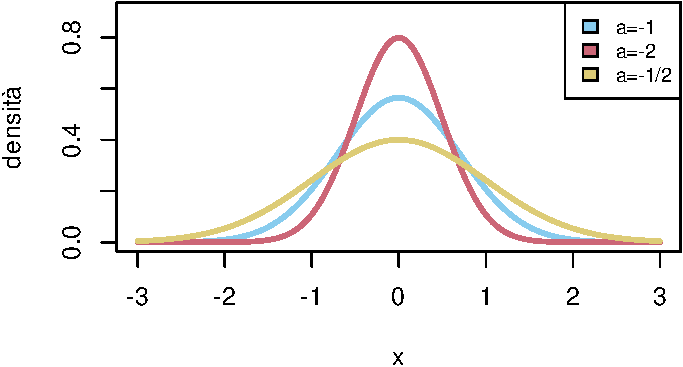
\includegraphics[keepaspectratio]{05-VA_gaussiane_files/figure-pdf/unnamed-chunk-2-1.pdf}}

}

\caption{densità gaussiana al variare del parametro \(a<0\)}

\end{figure}%

Osserviamo subito che la densità è una funzione pari, e al crescere di
\(a\) assume con maggiore probabilità i valori vicino a \(x=0\) (che è
la mediana e pure il valor medio). Un po' come nel caso della densità
esponenziale, ci possiamo aspettare un legame tra \(a\) e l'inverso
della deviazione standard, tuttavia per ragioni di unità di misura
(\(a\) moltiplica il quadrato di \(x\)), il legame sarà piuttosto tra
\(a\) e l'inverso della varianza.

Possiamo inoltre studiare il ruolo del parametro \(b\) tenendo fisso
\(a\) (ad esempio per \(a=1\)) e considerando il grafico della densità
al variare di \(b\).

\begin{Shaded}
\begin{Highlighting}[]
\NormalTok{deltax}\OtherTok{=}\FloatTok{0.01}
\NormalTok{x }\OtherTok{=}\FunctionTok{seq}\NormalTok{(}\SpecialCharTok{{-}}\DecValTok{3}\NormalTok{,}\DecValTok{3}\NormalTok{,}\AttributeTok{by=}\NormalTok{deltax)}

\CommentTok{\# caso b=0}
\NormalTok{densita}\OtherTok{=} \FunctionTok{exp}\NormalTok{(}\SpecialCharTok{{-}}\NormalTok{x}\SpecialCharTok{\^{}}\DecValTok{2}\NormalTok{)}
\NormalTok{densita }\OtherTok{=}\NormalTok{ densita}\SpecialCharTok{/}\FunctionTok{sum}\NormalTok{(densita}\SpecialCharTok{*}\NormalTok{deltax)}

\FunctionTok{plot}\NormalTok{(x, densita, }\AttributeTok{type=}\StringTok{\textquotesingle{}l\textquotesingle{}}\NormalTok{, }\AttributeTok{xlab=}\StringTok{\textquotesingle{}x\textquotesingle{}}\NormalTok{, }\AttributeTok{ylab=}\StringTok{\textquotesingle{}densità\textquotesingle{}}\NormalTok{, }\AttributeTok{col=}\NormalTok{miei\_colori[}\DecValTok{1}\NormalTok{], }\AttributeTok{lwd=}\DecValTok{3}\NormalTok{)}

\CommentTok{\# caso b=2}
\NormalTok{densita}\OtherTok{=} \FunctionTok{exp}\NormalTok{(}\SpecialCharTok{{-}}\NormalTok{x}\SpecialCharTok{\^{}}\DecValTok{2}\SpecialCharTok{+}\DecValTok{2}\SpecialCharTok{*}\NormalTok{x)}
\NormalTok{densita }\OtherTok{=}\NormalTok{ densita}\SpecialCharTok{/}\FunctionTok{sum}\NormalTok{(densita}\SpecialCharTok{*}\NormalTok{deltax)}

\FunctionTok{lines}\NormalTok{(x, densita, }\AttributeTok{type=}\StringTok{\textquotesingle{}l\textquotesingle{}}\NormalTok{,  }\AttributeTok{col=}\NormalTok{miei\_colori[}\DecValTok{2}\NormalTok{], }\AttributeTok{lwd=}\DecValTok{3}\NormalTok{ )}


\CommentTok{\# caso b={-}2}
\NormalTok{densita}\OtherTok{=} \FunctionTok{exp}\NormalTok{(}\SpecialCharTok{{-}}\NormalTok{x}\SpecialCharTok{\^{}}\DecValTok{2{-}2}\SpecialCharTok{*}\NormalTok{x)}
\NormalTok{densita }\OtherTok{=}\NormalTok{ densita}\SpecialCharTok{/}\FunctionTok{sum}\NormalTok{(densita}\SpecialCharTok{*}\NormalTok{deltax)}

\FunctionTok{lines}\NormalTok{(x, densita, }\AttributeTok{type=}\StringTok{\textquotesingle{}l\textquotesingle{}}\NormalTok{,  }\AttributeTok{col=}\NormalTok{miei\_colori[}\DecValTok{3}\NormalTok{], }\AttributeTok{lwd=}\DecValTok{3}\NormalTok{)}

\FunctionTok{legend}\NormalTok{(}\StringTok{\textquotesingle{}topright\textquotesingle{}}\NormalTok{, }\AttributeTok{fill=}\NormalTok{miei\_colori[}\DecValTok{1}\SpecialCharTok{:}\DecValTok{3}\NormalTok{], }\AttributeTok{legend=}\FunctionTok{c}\NormalTok{(}\StringTok{"b=0"}\NormalTok{, }\StringTok{"b={-}2"}\NormalTok{, }\StringTok{"b=2"}\NormalTok{), }\AttributeTok{cex=}\FloatTok{0.8}\NormalTok{)}
\end{Highlighting}
\end{Shaded}

\begin{figure}[H]

{\centering \pandocbounded{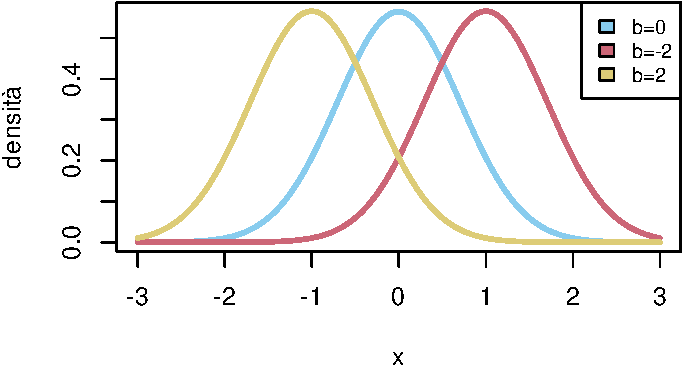
\includegraphics[keepaspectratio]{05-VA_gaussiane_files/figure-pdf/unnamed-chunk-3-1.pdf}}

}

\caption{densità gaussiana al variare del parametro \(b\)}

\end{figure}%

Vediamo dunque che al variare di \(b\) il grafico viene traslato verso
destra o sinistra (a seconda del segno). Ci aspettiamo quindi un legame
tra \(b\) e il valor medio di \(X\). La seguente proposizione rende
queste intuizioni precise.

Sia \(X\) una variabile con densità gaussiana
\[ p(X=x) \propto \exp\bra{ ax^2 +bx}.\] Allora vale
\[ a = -\frac{1}{2 \sigma_X^2}, \quad b = \frac{\E{X}}{\sigma_X^2},\]
ossia
\[ \Var{X} = \sigma_X^2 =  -\frac{1}{2a} \quad \E{X} = - \frac{b}{2a}.\]

\begin{proof}
Consideriamo l'integrale che definisce il valor medio e integriamo per
parti \[ \begin{split} \E{X} & = \int_{-\infty }^\infty x p(X=x) d x \\
& =  \int_{-\infty }^\infty x  c e^{ ax^2 +bx} d x \\
& = \int_{-\infty}^\infty \bra{  \frac{1}{2a} \frac{d}{dx} e^{a x^2} } c e^{bx} dx \\
& = - \frac 1 {2a } \int_{-\infty}^\infty e^{a x^2} \frac{d}{dx} \bra{ c  e^{bx}} d x\\
& =  - \frac b {2a } \int_{-\infty}^\infty  c e^{a x^2 + b} dx = \\
& = - \frac {b}{2a}.\end{split}\] Per la varianza, il calcolo è analogo
e lo riportiamo per semplicità solo nel caso \(b=0\), in modo che
\(\E{X}=  0\) e \(\Var{X} = \E{X^2}\):
\[ \begin{split} \E{X^2} & = \int_{-\infty }^\infty x^2 p(X=x) d x \\
& =  \int_{-\infty }^\infty x^2 c e^{ ax^2} d x \\
& = \int_{-\infty}^\infty \bra{  \frac{1}{2a} \frac{d}{dx} e^{a x^2} }  x dx \\
& = - \frac 1 {2a } \int_{-\infty}^\infty e^{a x^2} \frac{d}{dx} x d x\\
& =  - \frac 1 {2a } \int_{-\infty}^\infty  c e^{a x^2} dx = \\
& = - \frac {1}{2a}.\end{split}\]
\end{proof}

Sfruttando l'identificazione dei parametri \(a\), \(b\) in termini di
valor medio e varianza (o deviazione standard), introduciamo quindi la
parametrizzazione basata direttamente su tali indicatori. Questa è più
comune rispetto alla prima che abbiamo proposto, ma spesso risulta più
difficile da ricordare (e a volte non è necessaria).

Si dice che \(X \in \R\) ha densità continua gaussiana di valor medio
\(m \in \R\) e varianza \(\sigma^2>0\), e si scrive brevemente
\(\mathcal{N}(m, \sigma^2)\), se
\[ p(X=x ) \propto \exp\bra{ - \frac1 2 \frac {(x-m)^2} {\sigma^2} }.\]
Più esplicitamente, si può mostrare che vale l'identità
\[ p(X=x) =  \exp\bra{ - \frac1 2 \frac {(x-m)^2} {\sigma^2} } \frac{1}{\sqrt{ 2 \pi \sigma^2}}.\]

Per mostrare che le definizioni coincidano, basta notare che sviluppando
il quadrato nella definizione usuale si trova una densità gaussiana
rispetto alla prima definizione con
\[ a = -\frac{1}{2 \sigma^2} \quad b = \frac{m}{\sigma^2},\] e quindi
per la Proposizione si ha che \(m = \E{X}\), \(\sigma^2 = \Var{X}\). Per
ottenere la formula esplicita della densità si tratta di imporre che
l'integrale su tutto \(\R\) valga \(1\). Il termine più rilevante è su
cui vale la pena di concentrarsi è il fattore
\(1/\sqrt{\sigma^2} = 1/\sigma\), che dipende dal parametro di
deviazione standard \(\sigma\) e fa in modo che l'unità di misura sia
quella corretta. Il termine \(1/\sqrt{2 \pi}\) (che sembra un po'
misterioso) è in effetti una costante interessante da calcolare
analiticamente, ma non così rilevante ai fini pratici.

\begin{Shaded}
\begin{Highlighting}[]
\NormalTok{deltax}\OtherTok{=}\FloatTok{0.01}
\NormalTok{x }\OtherTok{=}\FunctionTok{seq}\NormalTok{(}\SpecialCharTok{{-}}\DecValTok{5}\NormalTok{,}\DecValTok{5}\NormalTok{,}\AttributeTok{by=}\NormalTok{deltax)}

\CommentTok{\# stavolta usiamo direttamente il comando dnorm() per ottenere la densità della gaussiana (l\textquotesingle{}unica accortezza è che R usa come parametro sigma e non la varianza sigma\^{}2)}

\CommentTok{\# caso m=0}
\NormalTok{densita}\OtherTok{=} \FunctionTok{dnorm}\NormalTok{(x, }\AttributeTok{mean=}\DecValTok{0}\NormalTok{, }\AttributeTok{sd=}\DecValTok{1}\NormalTok{)}

\FunctionTok{plot}\NormalTok{(x, densita, }\AttributeTok{type=}\StringTok{\textquotesingle{}l\textquotesingle{}}\NormalTok{, }\AttributeTok{xlab=}\StringTok{\textquotesingle{}x\textquotesingle{}}\NormalTok{, }\AttributeTok{ylab=}\StringTok{\textquotesingle{}densità\textquotesingle{}}\NormalTok{, }\AttributeTok{lwd=}\DecValTok{3}\NormalTok{, }\AttributeTok{col=}\NormalTok{miei\_colori[}\DecValTok{1}\NormalTok{] )}

\CommentTok{\# caso m=2}

\NormalTok{densita}\OtherTok{=} \FunctionTok{dnorm}\NormalTok{(x, }\AttributeTok{mean=}\DecValTok{2}\NormalTok{, }\AttributeTok{sd=}\DecValTok{1}\NormalTok{)}
\FunctionTok{lines}\NormalTok{(x, densita, }\AttributeTok{type=}\StringTok{\textquotesingle{}l\textquotesingle{}}\NormalTok{,  }\AttributeTok{col=}\NormalTok{miei\_colori[}\DecValTok{2}\NormalTok{], }\AttributeTok{lwd=}\DecValTok{3}\NormalTok{ )}


\CommentTok{\# caso m={-}2}
\NormalTok{densita}\OtherTok{=} \FunctionTok{dnorm}\NormalTok{(x, }\AttributeTok{mean=}\SpecialCharTok{{-}}\DecValTok{2}\NormalTok{, }\AttributeTok{sd=}\DecValTok{1}\NormalTok{)}


\FunctionTok{lines}\NormalTok{(x, densita, }\AttributeTok{type=}\StringTok{\textquotesingle{}l\textquotesingle{}}\NormalTok{,  }\AttributeTok{col=}\NormalTok{miei\_colori[}\DecValTok{3}\NormalTok{], }\AttributeTok{lwd=}\DecValTok{3}\NormalTok{)}

\FunctionTok{legend}\NormalTok{(}\StringTok{\textquotesingle{}topright\textquotesingle{}}\NormalTok{, }\AttributeTok{fill=}\NormalTok{miei\_colori[}\DecValTok{1}\SpecialCharTok{:}\DecValTok{3}\NormalTok{], }\AttributeTok{legend=}\FunctionTok{c}\NormalTok{(}\StringTok{"N(0,1)"}\NormalTok{, }\StringTok{"N(2,1)"}\NormalTok{, }\StringTok{"N({-}2,1)"}\NormalTok{), }\AttributeTok{cex=}\FloatTok{0.8}\NormalTok{)}
\end{Highlighting}
\end{Shaded}

\begin{figure}[H]

{\centering \pandocbounded{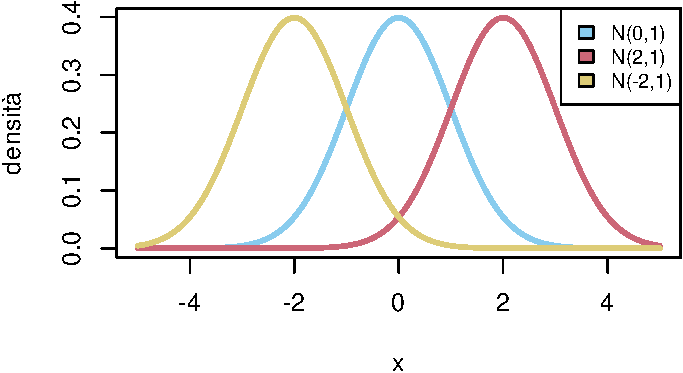
\includegraphics[keepaspectratio]{05-VA_gaussiane_files/figure-pdf/unnamed-chunk-4-1.pdf}}

}

\caption{densità gaussiana al variare del parametro \(m\) (con
\(\sigma=1\) costante}

\end{figure}%

\begin{Shaded}
\begin{Highlighting}[]
\NormalTok{deltax}\OtherTok{=}\FloatTok{0.01}
\NormalTok{x }\OtherTok{=}\FunctionTok{seq}\NormalTok{(}\SpecialCharTok{{-}}\DecValTok{5}\NormalTok{,}\DecValTok{5}\NormalTok{,}\AttributeTok{by=}\NormalTok{deltax)}

\CommentTok{\# stavolta usiamo direttamente il comando dnorm() per ottenere la densità della gaussiana (l\textquotesingle{}unica accortezza è che R usa come parametro sigma e non la varianza sigma\^{}2)}

\CommentTok{\# caso sigma=1}
\NormalTok{densita}\OtherTok{=} \FunctionTok{dnorm}\NormalTok{(x, }\AttributeTok{mean=}\DecValTok{0}\NormalTok{, }\AttributeTok{sd=}\DecValTok{1}\NormalTok{)}

\FunctionTok{plot}\NormalTok{(x, densita, }\AttributeTok{type=}\StringTok{\textquotesingle{}l\textquotesingle{}}\NormalTok{, }\AttributeTok{xlab=}\StringTok{\textquotesingle{}x\textquotesingle{}}\NormalTok{, }\AttributeTok{ylab=}\StringTok{\textquotesingle{}densità\textquotesingle{}}\NormalTok{, }\AttributeTok{ylim=}\FunctionTok{c}\NormalTok{(}\DecValTok{0}\NormalTok{,}\FloatTok{0.8}\NormalTok{), }\AttributeTok{col=}\NormalTok{miei\_colori[}\DecValTok{1}\NormalTok{], }\AttributeTok{lwd=}\DecValTok{3}\NormalTok{ )}

\CommentTok{\# caso sigma=2}

\NormalTok{densita}\OtherTok{=} \FunctionTok{dnorm}\NormalTok{(x, }\AttributeTok{mean=}\DecValTok{0}\NormalTok{, }\AttributeTok{sd=}\DecValTok{1}\SpecialCharTok{/}\DecValTok{2}\NormalTok{)}
\FunctionTok{lines}\NormalTok{(x, densita, }\AttributeTok{type=}\StringTok{\textquotesingle{}l\textquotesingle{}}\NormalTok{,  }\AttributeTok{col=}\NormalTok{miei\_colori[}\DecValTok{2}\NormalTok{], }\AttributeTok{lwd=}\DecValTok{3}\NormalTok{ )}


\CommentTok{\# caso sigma=1/2}
\NormalTok{densita}\OtherTok{=} \FunctionTok{dnorm}\NormalTok{(x, }\AttributeTok{mean=}\DecValTok{0}\NormalTok{, }\AttributeTok{sd=}\DecValTok{2}\NormalTok{)}


\FunctionTok{lines}\NormalTok{(x, densita, }\AttributeTok{type=}\StringTok{\textquotesingle{}l\textquotesingle{}}\NormalTok{,  }\AttributeTok{col=}\NormalTok{miei\_colori[}\DecValTok{3}\NormalTok{], }\AttributeTok{lwd=}\DecValTok{3}\NormalTok{)}

\FunctionTok{legend}\NormalTok{(}\StringTok{\textquotesingle{}topright\textquotesingle{}}\NormalTok{, }\AttributeTok{fill=}\NormalTok{miei\_colori[}\DecValTok{1}\SpecialCharTok{:}\DecValTok{3}\NormalTok{], }\AttributeTok{legend=}\FunctionTok{c}\NormalTok{(}\StringTok{"N(0,1)"}\NormalTok{, }\StringTok{"N(0,1/4)"}\NormalTok{, }\StringTok{"N(0,4)"}\NormalTok{), }\AttributeTok{cex=}\FloatTok{0.8}\NormalTok{)}
\end{Highlighting}
\end{Shaded}

\begin{figure}[H]

{\centering \pandocbounded{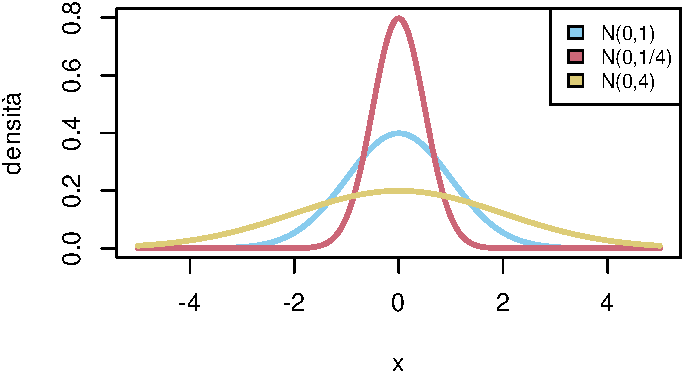
\includegraphics[keepaspectratio]{05-VA_gaussiane_files/figure-pdf/unnamed-chunk-5-1.pdf}}

}

\caption{densità gaussiana al variare del parametro \(\sigma\) (con
\(m=0\) costante}

\end{figure}%

\begin{remark}
La densità gaussiana è identificata dai due parametri di valor medio
\(m\) e varianza \(\sigma^2\). Si può mostrare che, al variare di tutte
le possibili densità continue per una variabile \(X\), \(p(X=x)\), con
\(x \in \R\), tali che il valor medio e la varianza di \(X\) siano
fissati
\[ \E{X} = \int_{-\infty}^\infty x P(X=x) d x = m, \quad \Var{X} = \int_{-\infty}^\infty (x-m)^2 P(X=x) d x = \sigma^2,\]
la densità gaussiana \(\mathcal{N}(m,\sigma^2)\) è quella di
\textbf{massima entropia}. Pertanto, seguento principio di massima
entropia, il robot, avendo a disposizione come informazione su una
variabile aleatoria (reale) solamente il suo valor medio \(m\) e la
varianza \(\sigma^2\), imporrà che sia una densità gaussiana
\(\mathcal{N}(m,\sigma^2)\).
\end{remark}

Un'applicazione della formula di cambio di variabile per densità
continua permette di ottenere il seguente risultato.

Sia \(X\) una variabile con densità continua
\(\mathcal{N}(m, \sigma^2)\) e siano \(\lambda\neq 0\), \(c \in \R\).
Allora la variabile \(Y = \lambda X +c\) ha densità continua gaussiana,
di parametri \(\mathcal{N}(\lambda m+c, \lambda^2\sigma^2)\).

Si può anche ricordarlo solo così: \emph{trasformazioni lineari affini
di variabili con densità gaussiana hanno densità gaussiana}, perché per
ottenere parametri di media e varianza basta ricordare il caso generale.

\begin{proof}
Applicando la formula di cambio di variabile con
\(g(x) = \lambda x +c\), essendo \(g'(x) = \lambda\),
\(g^{-1}(y) = (y-c)/\lambda\), si trova che
\[ p(Y=y) = p( X = (y-c)/\lambda ) \cdot \frac{1}{|\lambda|}.\]
\end{proof}

In particolare, se \(X\) ha densità gaussiana
\(\mathcal{N}(m,\sigma^2)\), la sua standardizzata
\[ \frac{X-m}{\sigma} \quad \text{ha densità continua $\mathcal{N}(0, 1)$,}\]
pertanto detta anche densità \textbf{gaussiana standard}, che ha densità
\[ \exp\bra{ - \frac 1 2 x^2 }\frac{1}{\sqrt{2 \pi}} \quad \text{per $x \in \R$.}\]

\begin{remark}
Nel caso \(\lambda = 0\), la variabile \(\lambda X + c = c\) è costante.
Per uniformare le notazioni, si conviene di considerare anche le
variabili costanti come caso \emph{degenere} di una densità gaussiana.
Nel caso vettoriale vedremo che una convenzione simile sarà anche più
utile.
\end{remark}

La funzione di ripartizione gaussiana (anche nel caso standard) non è
esprimibile in termini di funzioni elementari. Il comando R per
ottenerne i valori è \texttt{pnorm()}.

\begin{Shaded}
\begin{Highlighting}[]
\NormalTok{deltax}\OtherTok{=}\FloatTok{0.01}
\NormalTok{x }\OtherTok{=}\FunctionTok{seq}\NormalTok{(}\SpecialCharTok{{-}}\DecValTok{5}\NormalTok{,}\DecValTok{5}\NormalTok{,}\AttributeTok{by=}\NormalTok{deltax)}

\NormalTok{CDF }\OtherTok{=} \FunctionTok{pnorm}\NormalTok{(x)}

\FunctionTok{plot}\NormalTok{(x, CDF, }\AttributeTok{type=}\StringTok{\textquotesingle{}l\textquotesingle{}}\NormalTok{, }\AttributeTok{lwd=}\DecValTok{3}\NormalTok{, }\AttributeTok{col=}\NormalTok{miei\_colori[}\DecValTok{2}\NormalTok{])}
\end{Highlighting}
\end{Shaded}

\begin{figure}[H]

{\centering \pandocbounded{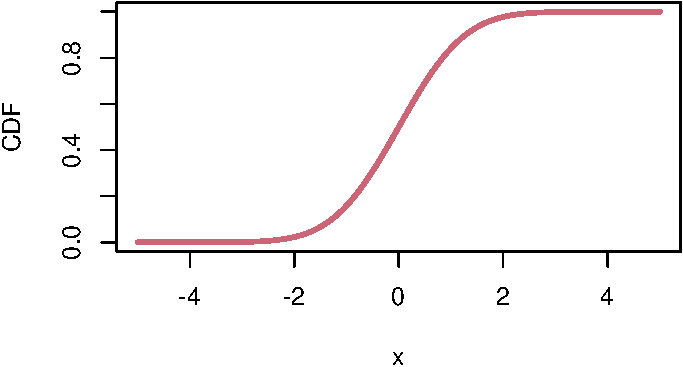
\includegraphics[keepaspectratio]{05-VA_gaussiane_files/figure-pdf/unnamed-chunk-6-1.pdf}}

}

\caption{CDF di una variabile gaussiana standard}

\end{figure}%

Si può invece calcolare esplicitamente la funzione generatrice dei
momenti e la funzione caratteristica di una qualsiasi variabile
gaussiana, che possono essere utili per ottenere i momenti di ordine
superiore al secondo.

Sia \(X\) una variabile con densità continua
\(\mathcal{N}(m, \sigma^2)\). Allora
\[ \operatorname{MGF}_X(t) = \exp\bra{ mt + \frac{\sigma^2}{2} t^2},\] e
\[ \varphi_X(\xi) = \exp\bra{ im\xi - \frac{\sigma^2}{2} \xi^2}.\]

\begin{proof}
Diamo la dimostrazione solo nel caso della MGF (la funzione
caratteristica segue formalmente ponendo \(i \omega\) al posto di
\(t\)).

Scrivendo \(X = \sigma X' + m\), dove \(X'\) è la standardizzata di
\(X\) e quindi ha densità gaussiana \(\mathcal{N}(0,1)\), si ha
\[ \operatorname{MGF}_X(t ) =\operatorname{MGF}_{\sigma X' +m} (t ) = \operatorname{MGF}_{X'}(\sigma t) e^{tm}.\]
Possiamo quindi ridurci al caso di una gaussiana standard
\(\mathcal{N}(0,1)\). Scrivendo l'integrale in questione si trova che la
MGF è
\[\begin{split} \int_{-\infty}^\infty e^{tx} e^{- \frac{ x^2}{2}} \frac{d x}{\sqrt{ 2 \pi}} & = \int_{-\infty}^\infty \exp\bra{- \frac 1 2 \bra{ - 2 tx +x^2 }} \frac{d x}{\sqrt{ 2 \pi}}\\
& = e^{\frac {t^2}{2}} \int_{-\infty}^\infty \exp\bra{- \frac 1 2 \bra{ t^2 - 2 tx +x^2 }} \frac{d x}{\sqrt{ 2 \pi}}\\
&  = e^{\frac {t^2}{2}} \int_{-\infty}^\infty \exp\bra{- \frac 1 2 \bra{ t-x}^2  } \frac{d x}{\sqrt{ 2 \pi}}\\
& = e^{\frac {t^2}{2}},
\end{split}\] dove l'ultimo integrale vale \(1\) perché riconosciamo una
densità \(\mathcal{N}(t,1)\).
\end{proof}

\subsection{Esercizi}\label{esercizi-25}

Usando il comando \(pnorm()\), verificare la ``regola'' del
\(68\)-\(95\)-\(99.7\), ossia mostrare che con probabilità del \(68\%\)
circa una variabile gaussiana \(\mathcal{N}(m, \sigma^2)\) assume valori
nell'intervallo \([m-\sigma, m+\sigma]\), con probabilità \(95\%\)
nell'intervallo \([m-2\sigma, m+2 \sigma]\) e infine con probabilità
\(99.7\%\) nell'intervallo \([m-3\sigma, m+3\sigma]\).

Mostrare che il quantile di una densità gaussiana standard
\(q: (0,1) \to \R\) soddisfa l'identità \(q(1-\alpha) = -q(\alpha)\) per
ogni \(\alpha \in (0,1)\). Verificarlo anche mediante plot usando il
comando \texttt{qnorm()}.

Calcolare il momento terzo e quarto di una variabile con densità
gaussiana standard e successivamente anche nel caso di una densità
gaussiana generale \(\mathcal{N}(m, \sigma^2)\).

\section{Il caso vettoriale}\label{sec-vettoriale}

Avendo descritto il caso delle variabili reali con densità gaussiana,
l'estensione al caso vettoriale è una generalizzazione, tecnica, ma
tutto sommato diretta. Possiamo quindi iniziare dando la seguente
definizione.

Si dice che una variabile aleatoria \(X \in \R^d\) ha densità continua
gaussiana se vale
\[ p(X=x) \propto \exp\bra{ \sum_{i,j=1}^d a_{ij} x_i x_j + \sum_{i=1}^d b_ix_i}, \quad \text{per ogni $x = (x_1, \ldots, x_d) \in \R^d$,}\]
per degli opportuni parametri
\(a = (a_{ij})_{i,j=1}^d \in \R^{d\times d}\),
\(b = (b_i)_{i=1}^d \in \R^d\).

Stavolta il (multi-)parametro \(a = (a_{ij})_{i,j=1}^d\) corrisponde ad
una matrice e \(b = (b_i)_{i=1}^d \in \R^d\) è un vettore. Sfruttando il
calcolo matriciale e il prodotto scalare possiamo scrivere in forma
compatta
\[\sum_{i,j=1}^d a_{ij} x_i x_j + \sum_{i=1}^d b_ix_i =  x \cdot (ax) + b \cdot x.\]
Possiamo anche supporre \(a\) simmetrica (la parte simmetrica non
darebbe alcun contributo) e definita positiva (altrimenti integrando su
tutto \(\R^d\) non si ottiene un integrale finito).

Come nel caso reale, ma con un po' più di calcoli (che omettiamo) si può
ottenere una formula che collega i parametri \(a\), \(b\) con la matrice
delle covarianze e il vettore dei valor medi di \(X\).

Sia \(X \in \R^d\) una variabile con densità gaussiana definita come
sopra. Allora la matrice delle covarianze \(\Sigma_X\) è definita
positiva (quindi invertibile) e vale
\[ a = -\frac{1}{2}\Sigma_X^{-1}, \quad b = \Sigma_X^{-1}\E{X},\] ossia
\[ \Sigma_X =  -\frac{1}{2} a^{-1} \quad \E{X} = -\frac 1 2 a^{-1} b .\]

La formula della densità si può quindi riscrivere in termini di
\(m =\E{X} \in \R^d\) e \(\Sigma_X \in \R^{d\times d}\), in modo analogo
al caso reale.

Si dice che \(X \in \R^d\) ha densità continua gaussiana di vettore dei
valor medi \(m \in \R^d\) e matrice delle covarianze \(\Sigma>0\), e si
scrive brevemente \(\mathcal{N}(m, \Sigma)\), se vale
\[ p(X=x ) \propto \exp\bra{ - \frac 1 2\bra{ (x-m)\cdot \Sigma^{-1} (x-m)} }.\]
Più esplicitamente, si può mostrare che vale l'identità
\[ p(X=x) =  \exp\bra{ - \frac1 2\bra{ (x-m) \cdot  \Sigma^{-1} (x-m)} } \frac{1}{\sqrt{ (2 \pi)^d \det(\Sigma)}}.\]

Come visualizzare una densità gaussiana vettoriale? Nel caso
bidimensionale \(d=2\), possiamo usare una \emph{heatmap} (mappa del
calore) in cui si rappresentano i valori della densità come colori
(colori luminosi corrispondono tipicamente a valori alti della densità,
ma è sempre bene affiancare una scala esplicativa).

\begin{Shaded}
\begin{Highlighting}[]
\NormalTok{deltax}\OtherTok{=}\FloatTok{0.1}
\NormalTok{deltay}\OtherTok{=}\FloatTok{0.1}

\NormalTok{x}\OtherTok{=} \FunctionTok{seq}\NormalTok{(}\SpecialCharTok{{-}}\DecValTok{3}\NormalTok{,}\DecValTok{3}\NormalTok{, }\AttributeTok{by=}\NormalTok{deltax)}
\NormalTok{y}\OtherTok{=}\FunctionTok{seq}\NormalTok{(}\SpecialCharTok{{-}}\DecValTok{3}\NormalTok{,}\DecValTok{3}\NormalTok{, }\AttributeTok{by=}\NormalTok{deltay)}

\NormalTok{N\_y }\OtherTok{=} \FunctionTok{length}\NormalTok{(y)}
\NormalTok{N\_x }\OtherTok{=} \FunctionTok{length}\NormalTok{(x)}

\CommentTok{\# creiamo una matrice con i valori della densità}
\NormalTok{densita }\OtherTok{=} \FunctionTok{matrix}\NormalTok{( }\DecValTok{0}\NormalTok{, }\AttributeTok{nrow =}\NormalTok{ N\_y, }\AttributeTok{ncol =}\NormalTok{N\_x)}

\ControlFlowTok{for}\NormalTok{ (i }\ControlFlowTok{in} \DecValTok{1}\SpecialCharTok{:}\NormalTok{N\_x  )\{}
  \ControlFlowTok{for}\NormalTok{ (j }\ControlFlowTok{in} \DecValTok{1}\SpecialCharTok{:}\NormalTok{N\_y)\{}
\NormalTok{    densita[i,j]}\OtherTok{=} \FunctionTok{exp}\NormalTok{(}\SpecialCharTok{{-}}\NormalTok{(x[i]}\SpecialCharTok{\^{}}\DecValTok{2}\SpecialCharTok{+}\NormalTok{y[j]}\SpecialCharTok{\^{}}\DecValTok{2}\NormalTok{)}\SpecialCharTok{/}\DecValTok{2}\NormalTok{) }\SpecialCharTok{/}\NormalTok{(}\DecValTok{2} \SpecialCharTok{*}\NormalTok{pi)}
\NormalTok{  \}}
\NormalTok{\}}

\CommentTok{\# usiamo image() per produrre il grafico (lo mostriamo solo perché è un comando generale per plottare una matrice). In alternativa si può anche usare filled.contour(), come vedremo nel prossimo esempio. Usiamo una scala di colori studiata perché sia accessibile anche alle persone che hanno difficoltà a percepire i colori.}


\FunctionTok{library}\NormalTok{(viridis)}
\end{Highlighting}
\end{Shaded}

\begin{verbatim}
Loading required package: viridisLite
\end{verbatim}

\begin{Shaded}
\begin{Highlighting}[]
\FunctionTok{image}\NormalTok{(x, y, densita, }\AttributeTok{col=}\FunctionTok{viridis}\NormalTok{(}\DecValTok{20}\NormalTok{))}
\end{Highlighting}
\end{Shaded}

\begin{figure}[H]

{\centering \pandocbounded{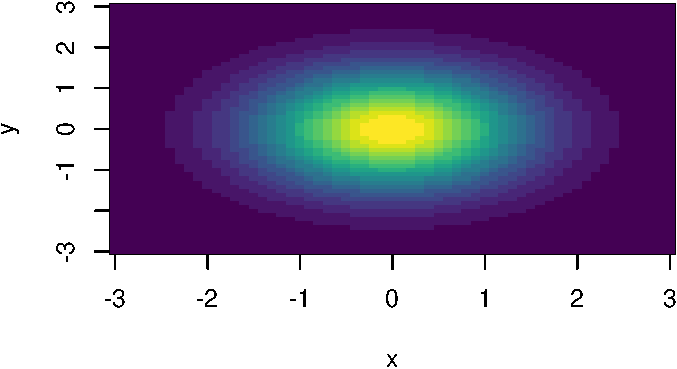
\includegraphics[keepaspectratio]{05-VA_gaussiane_files/figure-pdf/unnamed-chunk-7-1.pdf}}

}

\caption{visualizzazione della densità gaussiana vettoriale per \(d=2\),
\(m=0\) e \(\Sigma=Id\)}

\end{figure}%

Cosa accade se cambiamo la matrice di covarianza? la figura sotto mostra
il caso di
\[ \Sigma = \bra{ \begin{array}{cc} 2 & 1 \\ 1 & 1 \end{array} }.\]

\begin{Shaded}
\begin{Highlighting}[]
\CommentTok{\#usiamo la libreria mvtnorm per le densità gaussiani vettoriali generali (così non dobbiamo scrivere la formula esplicita)}


\FunctionTok{library}\NormalTok{(}\StringTok{\textquotesingle{}mvtnorm\textquotesingle{}}\NormalTok{)}

\CommentTok{\# definiamo il vettore dei valor medi m e la matrice di covarianza K}

\NormalTok{m }\OtherTok{=} \FunctionTok{c}\NormalTok{(}\DecValTok{0}\NormalTok{,}\DecValTok{0}\NormalTok{)}
\NormalTok{K }\OtherTok{=} \FunctionTok{matrix}\NormalTok{( }\FunctionTok{c}\NormalTok{(}\DecValTok{2}\NormalTok{,}\DecValTok{1}\NormalTok{,}\DecValTok{1}\NormalTok{,}\DecValTok{1}\NormalTok{), }\AttributeTok{nrow=}\DecValTok{2}\NormalTok{)}



\NormalTok{deltax}\OtherTok{=}\FloatTok{0.1}
\NormalTok{deltay}\OtherTok{=}\FloatTok{0.1}

\NormalTok{x}\OtherTok{=} \FunctionTok{seq}\NormalTok{(}\SpecialCharTok{{-}}\DecValTok{3}\NormalTok{,}\DecValTok{3}\NormalTok{, }\AttributeTok{by=}\NormalTok{deltax)}
\NormalTok{y}\OtherTok{=}\FunctionTok{seq}\NormalTok{(}\SpecialCharTok{{-}}\DecValTok{3}\NormalTok{,}\DecValTok{3}\NormalTok{, }\AttributeTok{by=}\NormalTok{deltay)}

\NormalTok{N\_x }\OtherTok{=} \FunctionTok{length}\NormalTok{(x)}
\NormalTok{N\_y }\OtherTok{=} \FunctionTok{length}\NormalTok{(y)}


\CommentTok{\# creiamo una matrice con i valori della densità}

\NormalTok{densita }\OtherTok{=} \FunctionTok{matrix}\NormalTok{( }\DecValTok{0}\NormalTok{, }\AttributeTok{nrow =}\NormalTok{ N\_y, }\AttributeTok{ncol =}\NormalTok{N\_x)}

\ControlFlowTok{for}\NormalTok{ (i }\ControlFlowTok{in} \DecValTok{1}\SpecialCharTok{:}\NormalTok{N\_x  )\{}
  \ControlFlowTok{for}\NormalTok{ (j }\ControlFlowTok{in} \DecValTok{1}\SpecialCharTok{:}\NormalTok{N\_y)\{}
\NormalTok{    densita[i,j]}\OtherTok{=} \FunctionTok{dmvnorm}\NormalTok{(}\FunctionTok{c}\NormalTok{(x[i], y[j]), m, K)}
\NormalTok{  \}}
\NormalTok{\}}

\CommentTok{\# usiamo stavolta filled.contour() per produrre il grafico e la scala di valori accanto}

\FunctionTok{filled.contour}\NormalTok{(x, y, densita, }\AttributeTok{color.palette =}\NormalTok{ viridis, }\AttributeTok{xlab=}\StringTok{\textquotesingle{}x\textquotesingle{}}\NormalTok{, }\AttributeTok{ylab=}\StringTok{\textquotesingle{}y\textquotesingle{}}\NormalTok{)}
\end{Highlighting}
\end{Shaded}

\begin{figure}[H]

{\centering \pandocbounded{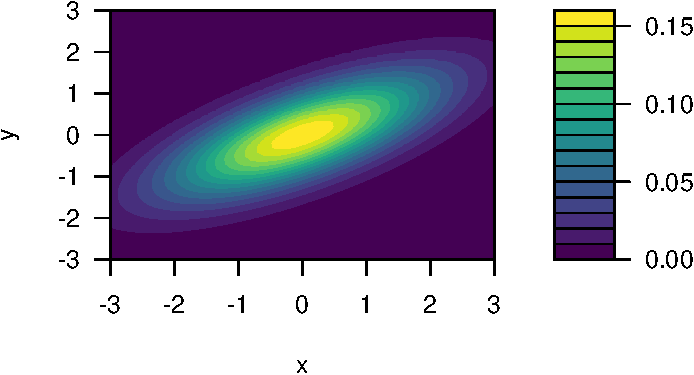
\includegraphics[keepaspectratio]{05-VA_gaussiane_files/figure-pdf/unnamed-chunk-8-1.pdf}}

}

\caption{visualizzazione della densità gaussiana vettoriale per \(d=2\),
\(m=0\) e \(\Sigma\) definita sopra}

\end{figure}%

Un modo alternativo è di rappresentare solamente una più ``curve di
livello'' della densità, ossia i punti del piano \((x,y) \in \R^2\) tali
che \(P((X,Y) = (x,y) ) = c\) per un fissato valore \(c>0\). Vediamo lo
stesso esempio di sopra (basta cambiare il comando per il plot).

\begin{Shaded}
\begin{Highlighting}[]
\CommentTok{\# usiamo contour() per produrre il grafico. Possiamo specificare quali livelli disegnare con l\textquotesingle{}opzione levels. Se non specificata R gestisce in automatico quali livelli rappresentare}

\FunctionTok{contour}\NormalTok{(x, y, densita, }\AttributeTok{col=}\NormalTok{miei\_colori[}\DecValTok{5}\NormalTok{], }\AttributeTok{lwd=}\DecValTok{2}\NormalTok{, }\AttributeTok{xlab=}\StringTok{\textquotesingle{}x\textquotesingle{}}\NormalTok{, }\AttributeTok{ylab=}\StringTok{\textquotesingle{}y\textquotesingle{}}\NormalTok{)}
\end{Highlighting}
\end{Shaded}

\begin{figure}[H]

{\centering \pandocbounded{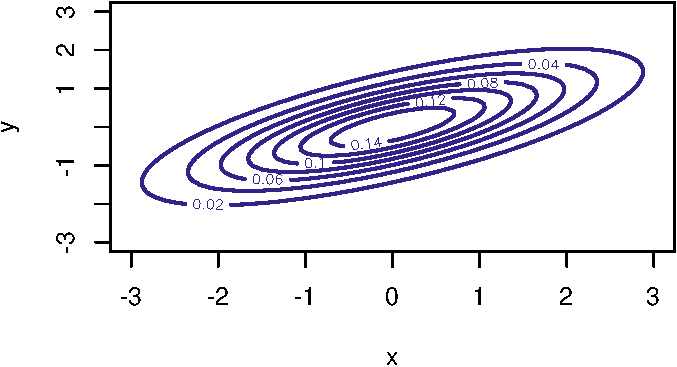
\includegraphics[keepaspectratio]{05-VA_gaussiane_files/figure-pdf/unnamed-chunk-9-1.pdf}}

}

\caption{visualizzazione della medesima densità gaussiana ma tramite
curve di livello}

\end{figure}%

\begin{remark}
Vediamo che gli insiemi di livello sono delle ellissi: questo si spiega
facilmente, perché l'insieme degli \(x\) tale che \(p(X=x) = c\)
coincide con quello di \(\log( p(X=x)) = \log c\), e poiché la densità
gaussiana è l'esponenziale di un polinomio di grado due (una ``forma
quadratica''), si trova l'equazione di una tra le figure geometriche
ellisse (o circonferenza), parabola o iperbole. Tuttavia le ultime due
non possono mai presentarsi, visto che la densità è infinitesima
all'infinito (si avrebbe altrimenti un valore \(c>0\) per alcuni \(x\)
arbitrariamente grandi).
\end{remark}

\begin{remark}
La densità gaussiana pure nel caso vettoriale è identificata dal vettore
dei valor medi \(m\) e dalla matrice delle covarianze \(\Sigma\).
Analogamente al caso reale, si può mostrare che essa è la densità di
massima entropia quando tali parametri sono fissati.
\end{remark}

Vediamo ora le proprietà principali per la densità gaussiana nel caso
vettoriale. La formula di cambio di variabile per densità continue
permette di mantenere densità gaussiane tramite mappe lineari affini.

Sia \(X \in \R^d\) una variabile con densità gaussiana
\(\mathcal{N}(m,\Sigma)\) e sia \(A \in \R^{k\times d}\),
\(b \in \R^k\). Allora, la variabile \(Y = AX+b\) ha densità gaussiana
\(\mathcal{N}(Am+b, A \Sigma A^T)\), purché \(A \Sigma A^T\) sia
invertibile (o, il che è lo stesso, definita positiva).

La condizione \(A \Sigma A^T\) definita positiva garantisce che la
densità esista. In realtà, come nel caso reale, è utile includere anche
i casi \emph{degeneri} in cui è solamente semi-definita positiva
(accenniamo come fare questa estensione verso la fine della sezione).
Per ora applicheremo il risultato senza preoccuparci di questa
condizione. Una prima conseguenza riguarda il caso di \(k=1\), ossia di
variabili gaussiane reali ottenute da un vettore aleatorio gaussiano (ad
esempio, le marginali).

Sia \(X \in \R^d\) una variabile con densità continua
\(\mathcal{N}(m, \Sigma)\). Allora 1. ogni marginale \(X_i\) ha densità
\(\mathcal{N}(m_i, \Sigma_{ii})\), 2. per ogni \(v \in \R^d\), la
variabile \(v \cdot X = \sum_{i=1}^d v_i X_i\) ha densità
\(\mathcal{N}(v \cdot m, v \cdot \Sigma v)\).

Ad esempio, se le due marginali \(X_1\), \(X_2\) di \(X\) sono non
correlate, sa ha che, ponendo \(v = (1,1,0,0,\ldots)\) la variabile
\(X_1+X_2\) ha densità
\(\mathcal{N}(m_1+m_2, \sigma_{X_1}^2 + \sigma_{X_2}^2)\).

Una conseguenza importante riguarda le variabili standardizzate.

Sia \(X \in \R^d\) una variabile con densità continua
\(\mathcal{N}(m, \Sigma)\). Allora la variabile standardizzata
\[ Z = \sqrt{D}^{-1} U (X-m) \quad \text{ha densità continua $\mathcal{N}(0, Id)$,}\]
detta anche \textbf{gaussiana standard} vettoriale. La densità esplicita
è piuttosto semplice e vale
\[ P(Z= z |  \mathcal{N}(0, Id)) = \exp\bra{ - \frac1 2 \sum_{i=1}^d z_i^2 }  \frac{1}{\sqrt{ (2 \pi)^d}}. \]

Notiamo che la densità si decompone come prodotto di densità gaussiane
standard reali (corrispondenti ai valori delle marginali):
\[ \exp\bra{ - \frac1 2 \sum_{i=1}^d z_i^2 }  \frac{1}{\sqrt{ (2 \pi)^d}} = \prod_{i=1}^d  \exp\bra{ - \frac1 2 z_i^2 }  \frac{1}{\sqrt{ 2 \pi}}.\]
Ne segue che le variabili marginali \(Z_1\), \(Z_2\), \ldots \(Z_d\)
sono \emph{indipendenti}, oltre ad essere non correlate. Per le
variabili con densità gaussiana l'indipendenza è praticamente
equivalente alla non correlazione: vale infatti il seguente risultato
(non vero in generale per variabili non gaussiane!).

Siano \(X \in \R^d\), \(Y \in \R^k\) variabili aleatorie indipendenti
con densità gaussiane. Allora la variabile congiunta
\((X,Y) \in \R^{d+k}\) ha densità gaussiana.

Viceversa, se la variabile congiunta \((X,Y) \in \R^{d+k}\) ha densità
gaussiana e \(\Cov{X_i,Y_j} = 0\) per ogni \(i\in \cur{1, \ldots, d}\),
\(j \in \cur{1, \ldots, k}\), allora \(X\) e \(Y\) sono indipendenti.

\begin{proof}
Nel primo caso, la densità congiunta è il prodotto delle densità
marginali. Usando la definizione veloce, scriviamo
\[p( (X,Y)=(x,y)) = p(X=x) p(Y=y) \propto \exp\bra{ x\cdot ax + b \cdot x} \exp\bra{ y \cdot a' y + b' \cdot y}\]
per opportuni (multi-)parametri \(a\), \(b\), \(a'\), \(b'\). Le
proprietà dell'esponenziale implicano la densità si scrive come
un'esponenziale di un polinomio di secondo grado nelle variabili
\(x=(x_i)_{i=1}^d\) e \(y=(y_j)_{j=1}^k\), pertanto è una densità
gaussiana.

Viceversa, se la variabile congiunta ha densità gaussiana e
\(\Cov{X_i, Y_j} = 0\), significa che la varianza \(\Sigma_{(X,Y)}\) ha
una struttura di matrice \emph{a blocchi},
\[ \Sigma_{(X,Y)} = \bra{ \begin{array}{cc} \Sigma_X & 0 \\ 0 & \Sigma_Y \end{array}}.\]
Ora si può mostrare che l'inversa \(\Sigma_{(X,Y)}^{-1}\) ha pure la
struttura a blocchi (nel caso \(2\times 2\) è immediato):
\[ \Sigma_{(X,Y)}^{-1} = \bra{ \begin{array}{cc} \Sigma_X^{-1} & 0 \\ 0 & \Sigma_Y^{-1} \end{array}}.\]
Perciò, il termine quadratico nella densità congiunta si spezza come
somma di due termini quadratici associati alle marginali:
\[ (x,y) \cdot \Sigma_{(X,Y)}^{-1}(x,y)  = x \cdot \Sigma_X^{-1} x + y \cdot \Sigma_Y ^{-1} y\]
e lo stesso per il termine lineare
\[ (m_X, m_Y) \cdot (x,y) = m_X \cdot x + m_Y \cdot y\] in conclusione,
la densità congiunta si spezza come prodotto di due densità marginali
\[ p( (X,Y)=(x,y)) \propto \exp\bra{ -\frac 1 2  x \cdot \Sigma_X^{-1} x  + m_X \cdot x} \exp\bra{ -\frac 1 2  y \cdot \Sigma_Y^{-1} y  + m_Y \cdot y} \]
e quindi vale l'indipendenza.
\end{proof}

Riprendendo l'esempio della somma delle marginali del vettore gaussiano,
segue che se \(X\), \(Y\) sono due variabili gaussiane reali
indipendenti, allora \((X, Y)\) è un vettore gaussiano e quindi la somma
delle marginali \(X+Y\) è gaussiana (reale) con i parametri naturali
(somma delle medie e somma delle varianze)
\(\mathcal{N}(m_X+m_Y, \sigma_{X}^2 + \sigma_{X}^2)\).

Dato un vettore gaussiano \((X,Y)\), non solo le marginali \(X\) e \(Y\)
hanno densità gaussiana, ma anche la densità condizionale di una
marginale, diciamo \(X\), rispetto all'altra (\(Y\)) è gaussiana, come
mostra la seguente proposizione (i parametri si possono anche calcolare
esplicitamente, ma non lo riportiamo per semplicità).

Sia \((X,Y) \in \R^{d+k}\) un vettore aleatorio con densità gaussiana.
Allora, per ogni \(y \in \R^k\), condizionatamente a \(\cur{Y=y}\), la
densità di \(X \in\R^d\) è gaussiana.

\begin{proof}
Ricordiamo che la densità condizionale si può ottenere dalla densità
congiunta ``congelando'' la variabile rispetto alla quale si condiziona
\(y\) (a essere precisi non si trova direttamente la densità, perché
bisognerebbe comunque moltiplicare per una costante opportuna, ma a noi
basterà questo, per riconoscere la densità gaussiana). È chiaro che, se
all'esponente abbiamo un polinomio di secondo grado nelle variabili
\(x\), e \(y\), fissando la \(y\) otterremo comunque un polinomio di
secondo grado nella \(x\). Pertanto non vi è dubbio che la densità
condizionale di \(X\) sapendo \(Y=y\) è gaussiana.
\end{proof}

Concludiamo con un risultato che riguarda la funzione generatrice dei
momenti e la funzione caratteristica di una variabile gaussiana nel caso
vettoriale.

Sia \(X \in \R^d\) una variabile con densità continua gaussiana
\(\mathcal{N}(m, \Sigma)\). Allora
\[ \operatorname{MGF}_X(t) = \exp\bra{ m\cdot t + \frac{1}{2} t \cdot \Sigma t},\]
e
\[ \varphi_X(\xi) = \exp\bra{ im\cdot\xi - \frac{1}{2} \xi \cdot \Sigma \xi}.\]

\begin{proof}
Basta notare che, fissato \(t \in \R^d\), la variabile reale
\(X\cdot t\) ha densità gaussiana di media \(m \cdot t\) e varianza
\(t \cdot \Sigma t\). Pertanto usando la \(\operatorname{MGF}\) già nota
nel caso delle variabili gaussiane reali, segue che
\[ \operatorname{MGF}_X(t) = \E{\exp\bra{ t \cdot X}}=\operatorname{MGF}_{X \cdot t} (1) = \exp\bra{ m\cdot t + \frac{1}{2} t \cdot \Sigma t}.\]
Similmente per la funzione caratteristica.
\end{proof}

\begin{remark}
Notiamo che sia la funzione generatrice dei momenti che la funzione
caratteristica sono esponenziali di polinomi di secondo grado nelle
variabili (\(t\) e \(\xi\) rispettivamente). Tuttavia, rispetto alla
densità, la matrice di covarianza \(\Sigma\) non è invertita, né il suo
determinante compare al denominatore (in effetti, proprio non compare).
Pertanto, le espressioni continuano ad avere senso anche nel caso
degenere, in cui \(\Sigma\) è semidefinita positiva (ma non
necessariamente invertibile). Ricordando che la funzione caratteristica
identifica in modo unico la legge di una variabile aleatoria (sia he
abbia densità, ma anche se non ce l'ha), questa espressione permette
allora di **definire* una variabile aleatoria vettoriale gaussiana anche
nel caso in cui non abbia densità continua. L'intepretazione in tali
casi è che la densità continua si concentra ``troppo'' in un sottospazio
affine di dimensione più bassa dello spazio ambiente \(\R^d\). Per
visualizzare cosa accade, diamo un plot nel caso ``quasi degenere''
ponendo ad esempio
\[ \Sigma = \bra{ \begin{array}{cc} 1 & 0.99 \\ 0.99 & 1\end{array}}.\]

\begin{Shaded}
\begin{Highlighting}[]
\CommentTok{\# definiamo il vettore dei valor medi m e la matrice di covarianza K}

\NormalTok{m }\OtherTok{=} \FunctionTok{c}\NormalTok{(}\DecValTok{1}\NormalTok{,}\DecValTok{1}\NormalTok{)}
\NormalTok{K }\OtherTok{=} \FunctionTok{matrix}\NormalTok{( }\FunctionTok{c}\NormalTok{(}\DecValTok{1}\NormalTok{,}\FloatTok{0.99}\NormalTok{,}\FloatTok{0.99}\NormalTok{,}\DecValTok{1}\NormalTok{), }\AttributeTok{nrow=}\DecValTok{2}\NormalTok{)}


\NormalTok{deltax}\OtherTok{=}\FloatTok{0.05}
\NormalTok{deltay}\OtherTok{=}\FloatTok{0.05}

\NormalTok{x}\OtherTok{=} \FunctionTok{seq}\NormalTok{(}\SpecialCharTok{{-}}\DecValTok{4}\NormalTok{,}\DecValTok{4}\NormalTok{, }\AttributeTok{by=}\NormalTok{deltax)}
\NormalTok{y}\OtherTok{=}\FunctionTok{seq}\NormalTok{(}\SpecialCharTok{{-}}\DecValTok{4}\NormalTok{,}\DecValTok{4}\NormalTok{, }\AttributeTok{by=}\NormalTok{deltay)}

\NormalTok{N\_x }\OtherTok{=} \FunctionTok{length}\NormalTok{(x)}
\NormalTok{N\_y }\OtherTok{=} \FunctionTok{length}\NormalTok{(y)}


\CommentTok{\# creiamo una matrice con i valori della densità}

\NormalTok{densita }\OtherTok{=} \FunctionTok{matrix}\NormalTok{( }\DecValTok{0}\NormalTok{, }\AttributeTok{nrow =}\NormalTok{ N\_y, }\AttributeTok{ncol =}\NormalTok{N\_x)}

\ControlFlowTok{for}\NormalTok{ (i }\ControlFlowTok{in} \DecValTok{1}\SpecialCharTok{:}\NormalTok{N\_x  )\{}
  \ControlFlowTok{for}\NormalTok{ (j }\ControlFlowTok{in} \DecValTok{1}\SpecialCharTok{:}\NormalTok{N\_y)\{}
\NormalTok{    densita[i,j]}\OtherTok{=} \FunctionTok{dmvnorm}\NormalTok{(}\FunctionTok{c}\NormalTok{(x[i], y[j]), m, K)}
\NormalTok{  \}}
\NormalTok{\}}


\FunctionTok{contour}\NormalTok{(x, y, densita, }\AttributeTok{levels=}\FunctionTok{c}\NormalTok{(}\FloatTok{0.001}\NormalTok{, }\FloatTok{0.01}\NormalTok{, }\FloatTok{0.1}\NormalTok{,}\DecValTok{1}\NormalTok{), }\AttributeTok{col=}\NormalTok{miei\_colori[}\DecValTok{5}\NormalTok{], }\AttributeTok{lwd=}\DecValTok{1}\NormalTok{, }\AttributeTok{xlab=}\StringTok{\textquotesingle{}x\textquotesingle{}}\NormalTok{, }\AttributeTok{ylab=}\StringTok{\textquotesingle{}y\textquotesingle{}}\NormalTok{)}
\end{Highlighting}
\end{Shaded}

\begin{figure}[H]

{\centering \pandocbounded{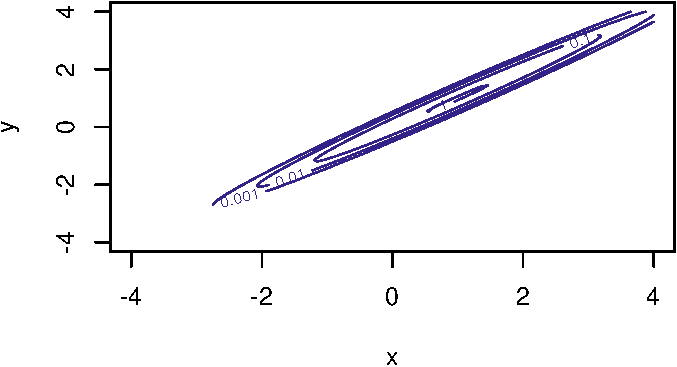
\includegraphics[keepaspectratio]{05-VA_gaussiane_files/figure-pdf/unnamed-chunk-10-1.pdf}}

}

\caption{rappresentazione della densità gaussiana vettoriale nel caso
vettoriale \(d=2\), \(m=(1,1)\) e \(\Sigma\) definita sopra}

\end{figure}%

\end{remark}

\subsection{Esercizi}\label{esercizi-26}

Dire se la matrice
\[ \Sigma = \bra{ \begin{array}{cc} 2 & -1 \\ -1 & 3 \end{array} }.\]
può essere la matrice di covarianza di una variabile gaussiana. In caso
affermativo, usare opportuni comandi R per visualizzare (come heatmap
oppure curve di livello) la densità.

Sia \((X,Y)\) un vettore aleatorio gaussiano a valori in \(\R^2\) con
valor medio \(m =(1,-2)\) e covarianza
\[ \Sigma = \bra{ \begin{array}{cc} 4 & -3 \\ -3 & 4 \end{array} }.\] -
Determinare la densità della variabile \(Z = X+2Y\). - Dire se la
variabile \((X,Z)\) è gaussiana e determinarne i parametri
\emph{(suggerimento scriverla come trasformazione lineare di
\((X,Y)\))}. - Usare opportuni comandi R per visualizzare la densità di
\((X,Y)\) e \((X,Z)\).

\section{Stima dei parametri da una singola
osservazione}\label{sec-stima}

Data una variabile aleatoria \(X \in \R^d\) con densità gaussiana
\(\mathcal{N}(m, \Sigma)\), come stimare i parametri basandosi
sull'osservazione di \(X\)? Come abbiamo visto nella Sezione
Sezione~\ref{sec-bayes-va}, tale problema può essere naturalmente
studiato dal punto di vista bayesiano, supponendo quindi che i parametri
\(m\), \(\Sigma\) siano delle variabili aleatorie con opportune densità
\emph{a priori}, e determinando quindi la densità avendo osservato
\(X=x\) tramite la formula di Bayes. A questo metodo si affianca
l'alternativa più diretta, ma meno informativa, di limitarsi ad una
stima di massima verosimiglianza.

Per illustrare il metodo, iniziamo con lo studio in questa sezione del
caso di una variabile aleatoria \(X \in \R\) di cui bisogna stimare i
parametri \(m\), \(\sigma^2\) sulla base della sola osservazione di
\(X\). Nella sezione successiva, generalizzeremo al caso in cui vi siano
più osservazioni e argomenteremo che la stima diverrà allora più
precisa.

Supponiamo in questa sezione che il robot abbia modellizato una quantità
aleatoria reale \(X \in \R\) come una variabile con densità gaussiana
\(\mathcal{N}(m,\sigma^2)\). I parametri non sono noti a priori, e
vengono stimati sulla base di una osservazione \(X=x\). Pertanto
seguendo il metodo bayesiano il robot introduce le rispettive variabili
aleatorie \(M\) per la media e \(V\) per la varianza (questa a valori
positivi).

La verosimiglianza, ossia la densità di \(X\) supponendo note la media
\(M=m\) e la varianza \$V = v \$ (usiamo la lettera \(v\) al posto di
\(\sigma^2\), per alleggerire la notazione) è quindi
\[ L( m,v; x) = p(X =x | M=m V=v) = \exp\bra{ - \frac 1 {2 v} (x-m)^2 }\frac{1}{\sqrt{ 2 \pi v}}.\]
È importante specificare tutta la densità (anche se il termine
\(\sqrt{2 \pi}\) non sarebbe rilevante), perché interessa la dipendenza
dai parametri \(m\) e \(v\). Possiamo rappresentare graficamente la
funzione dei due parametri \((m,v)\) con una heatmap.

\begin{Shaded}
\begin{Highlighting}[]
\NormalTok{deltam}\OtherTok{=}\FloatTok{0.1}
\NormalTok{deltav}\OtherTok{=}\FloatTok{0.05}

\NormalTok{m}\OtherTok{=} \FunctionTok{seq}\NormalTok{(}\DecValTok{0}\NormalTok{,}\DecValTok{2}\NormalTok{, }\AttributeTok{by=}\NormalTok{deltam)}
\NormalTok{v}\OtherTok{=}\FunctionTok{seq}\NormalTok{(}\FloatTok{0.01}\NormalTok{,}\FloatTok{0.5}\NormalTok{, }\AttributeTok{by=}\NormalTok{deltav)}

\NormalTok{N\_m }\OtherTok{=} \FunctionTok{length}\NormalTok{(m)}
\NormalTok{N\_v }\OtherTok{=} \FunctionTok{length}\NormalTok{(v)}

\CommentTok{\# osservazione}

\NormalTok{x}\OtherTok{=}\DecValTok{1}


\CommentTok{\# creiamo una matrice con i valori della verosimiglianza}

\NormalTok{L }\OtherTok{=} \FunctionTok{matrix}\NormalTok{( }\DecValTok{0}\NormalTok{, }\AttributeTok{nrow =}\NormalTok{ N\_m, }\AttributeTok{ncol =}\NormalTok{N\_v)}

\ControlFlowTok{for}\NormalTok{ (i }\ControlFlowTok{in} \DecValTok{1}\SpecialCharTok{:}\NormalTok{N\_m)\{}
  \ControlFlowTok{for}\NormalTok{ (j }\ControlFlowTok{in} \DecValTok{1}\SpecialCharTok{:}\NormalTok{N\_v)\{}
\NormalTok{    L[i,j]}\OtherTok{=} \FunctionTok{exp}\NormalTok{(}\SpecialCharTok{{-}}\NormalTok{(m[i]}\SpecialCharTok{{-}}\NormalTok{x)}\SpecialCharTok{\^{}}\DecValTok{2}\SpecialCharTok{/}\NormalTok{(}\DecValTok{2}\SpecialCharTok{*}\NormalTok{v[j])) }\SpecialCharTok{/} \FunctionTok{sqrt}\NormalTok{(}\DecValTok{2} \SpecialCharTok{*}\NormalTok{pi }\SpecialCharTok{*}\NormalTok{v[j])}
\NormalTok{  \}}
\NormalTok{\}}

\CommentTok{\# usiamo stavolta filled.contour() per produrre il grafico e la scala di valori accanto}

\FunctionTok{filled.contour}\NormalTok{(m, v, L, }\AttributeTok{color.palette=}\NormalTok{viridis, }\AttributeTok{xlab=}\StringTok{\textquotesingle{}m\textquotesingle{}}\NormalTok{, }\AttributeTok{ylab=}\StringTok{\textquotesingle{}v\textquotesingle{}}\NormalTok{)}
\end{Highlighting}
\end{Shaded}

\begin{figure}[H]

{\centering \pandocbounded{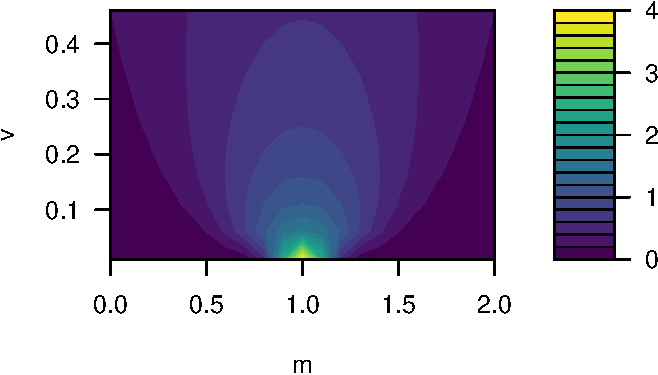
\includegraphics[keepaspectratio]{05-VA_gaussiane_files/figure-pdf/unnamed-chunk-11-1.pdf}}

}

\caption{verosimiglianza per \(M\) e \(V\) avendo osservato \(X=1\).}

\end{figure}%

\subsection{Stima di massima
verosimiglianza}\label{stima-di-massima-verosimiglianza}

Dal grafico sopra è evidente che la verosimiglianza \(L\) è massima per
\(m=x\) (in tal caso era \(X=1\)) e \(v=0\), un fatto che ora
giustifichiamo analiticamente, determinando la stima di massima
verosimiglianza per i parametri. Passando al logaritmo e moltiplicando
per \(-2\), invece di massimizzare \(L\) basta minimizzare la funzione
\[ (m,v) \mapsto  - 2 \log L(m,v; x) = \frac 1 { v} (x-m)^2  +  \log( 2 \pi v).\]
Derivando rispetto a \(m\) e imponendo che la derivata si annulli si
ottiene, per ogni \(v>0\),
\[ \frac 2 { v} (x-m)  =0 \quad \text{da cui $m=x$,} \] mentre se
deriviamo rispetto a \(v\), tenendo fisso \(m\), si trova
\[  -\frac 1 { v^2} (x-m)^2 + \frac{1}{v} = 0, \quad \text{da cui $v = (x-m)^2$. }\]
dovendo massimizzare congiuntamente si trova quindi la coppia
\(m_{{\mle}} =x\), \(v_{{\mle}} = 0\) (anche se, ad essere rigorosi, per
\(v=0\) non è ben definita la verosimiglianza).

Con calcoli analoghi a quanto fatto sopra si ottiene anche che 1. se il
parametro di varianza \(V=v_0 >0\) è noto (ossia \(V=v_0\) è costante
rispetto all'informazione a priori), allora la stima di massima
verosimiglianza per il parametro di media è \(m_{\mle} = x\) (qualsiasi
sia \(v_0\)). 2. se il parametro di media \(M=m_0 \in \R\) è noto (ossia
\(M=m_0\) è costante a priori), allora la stima di massima
verosimiglianza per il parametro di varianza è
\(v_{{\mle}} = (x-m_0)^2\).

\subsection{Stima bayesiana per la media, varianza
nota}\label{stima-bayesiana-per-la-media-varianza-nota}

Per applicare il metodo bayesiano, il robot deve proporre delle densità
\emph{a priori} per media \(M\) e varianza \(V\) che rappresentano
l'informazione di cui dispone prima di osservare \(X\), e applicare la
formula di Bayes per ottenere le densità condizionate a \(X=x\).
Ovviamente le densità a priori dipendono dalla natura dell'informazione
iniziale di cui dispone. La semplice rete bayesiana che rappresenta il
problema è rappresentata in figura.

\begin{figure}[H]

{\centering \pandocbounded{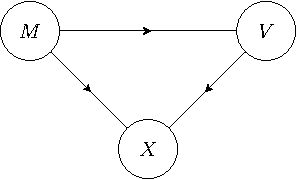
\includegraphics[keepaspectratio]{05-VA_gaussiane_files/figure-pdf/unnamed-chunk-12-1.pdf}}

}

\caption{Rete bayesiana tra le variabili \(M\), \(V\) e \(X\)}

\end{figure}%

Affrontiamo prima due casi estremi, in cui i risultati si possono
ottenere analiticamente, se si scelgono delle densità a priori
particolari: consideriamo prima il caso in cui \(V = v_0\) sia nota (e
quindi sia una variabile costante) e successivamente quello in cui
\(M = m_0\) sia invece nota. In questi casi si può rimuovere il nodo
corrispondente alle variabili costanti dalla rete bayesiana.

Supponendo che \(V=v_0\) sia costante, i calcoli risultano
particolarmente semplici se si suppone che \(M\) sia una variabile
gaussiana con parametri (noti) \(\mathcal{N}(m_0, \sigma_m^2)\), ossia
\[ p(M= m| \Omega) \propto \exp\bra{-\frac 1 {2\sigma_m^2} (m-m_0)^2}.\]
Questa densità codifica una informazione nota al robot riguardante il
parametro di media \(m\): esso è localizzato intorno al parametro
\(m_0\), con una dispersione (deviazione standard) \(\sigma_m\). Per
rappresentare maggiore incertezza su \(M\) è sufficiente far crescere
\(\sigma_m\), e nel limite \(\sigma_m \to \infty\) vedremo che si ricade
nella stima di massima verosimiglianza.

Avendo osservato \(X=x\), dalla formula di Bayes segue che la densità
per \(M\) è
\[ \begin{split} p(M=m| X=x) & \propto p(M=m|\Omega ) p(X =x | M=m, V=v_0) \\
& \propto \exp\bra{ -\frac 1 2 \bra{ \frac{ (m-m_0)^2}{\sigma_m^2} + \frac { (x-m)^2}{v_0} }}.\end{split}\]
Si tratta evidentemente di una nuova densità gaussiana essendo
l'esponenziale di un polinomio di secondo grado nella variabile \(m\).
Con semplici passaggi algebrici si ricavano i parametri di media e
varianza, che dipendono naturalmente dall'osservazione \(x\),
\[ m_{|X=x} = (1-\alpha) x + \alpha m_0, \quad \sigma^2_{m|X=x} = \sigma_m^2\alpha,\]
dove abbiamo posto, per semplicità,
\[\alpha = \frac{1}{1+\sigma_m^2/v_0 } \in (0,1).\] Osserviamo quindi
che la nuova informazione \(X=x\) ``sposta'' la fiducia del robot verso
il valore osservato \(x\), ma non completamente (come invece accade con
la massima verosimiglianza). Molto dipende dal valore di \(\alpha\),
ossia dal rapporto tra le varianze \(\sigma_m^2/v_0\) (entrambe note a
priori). I casi limite sono particolarmente rilevanti: 1. se
\(v_0<< \sigma_m^2\), allora \(\alpha \sim 0\) e ci si avvicina alla
stima di massima verosimiglianza (il che non stupisce perché
\(\sigma_m\) grande significa che la densità a priori per \(M\) era poco
informativa) 2. se \(v_0>> \sigma_m^2\), allora \(\alpha \sim 1\) e la
media \(m_{|X=x}\) rimane praticamente invariata, essenzialmente perché
l'informazione iniziale era molto precisa su \(M\), e una singola
osservazione non la modifica molto.

\subsection{Stima bayesiana per la varianza, media
nota}\label{stima-bayesiana-per-la-varianza-media-nota}

Supponiamo ora che \(M =m_0\) sia costante rispetto all'informazione
iniziale disponibile al robot e introduciamo una densità a priori per la
varianza \(V\). Uno dei problemi principali è che \(V\) deve essere
non-negativa, ma vi sono diverse scelte comode per ottenere risultati
analitici. Una di queste è una densità continua del tipo
\emph{esponenziale inversa}, ossia \(1/V\) è esponenziale con parametro
\(\lambda = v_0/2\) (dove \(v_0\) è un parametro che riteniamo noto
mentre il coefficiente \(1/2\) è solo per semplificare i calcoli). Dalla
formula di cambio di variabile si trova che
\[ p( V = v|\Omega)  \propto p(1/V = 1/v)\frac{1}{v^2} \propto \exp\bra{ -\frac{v_0}{2v}}\frac{1}{v^2}.\]

\begin{Shaded}
\begin{Highlighting}[]
\NormalTok{deltav}\OtherTok{=}\FloatTok{0.01}
\NormalTok{v}\OtherTok{=}\FunctionTok{seq}\NormalTok{(deltav, }\DecValTok{4}\NormalTok{, }\AttributeTok{by=}\NormalTok{deltav)}

\NormalTok{v\_0 }\OtherTok{=} \DecValTok{1}

\NormalTok{densita\_esp\_inv }\OtherTok{=} \FunctionTok{exp}\NormalTok{(}\SpecialCharTok{{-}}\NormalTok{(v\_0}\SpecialCharTok{/}\NormalTok{(}\DecValTok{2}\SpecialCharTok{*}\NormalTok{v)))}\SpecialCharTok{/}\NormalTok{v}\SpecialCharTok{\^{}}\DecValTok{2}
\NormalTok{densita\_esp\_inv }\OtherTok{=}\NormalTok{ densita\_esp\_inv}\SpecialCharTok{/}\FunctionTok{sum}\NormalTok{(densita\_esp\_inv }\SpecialCharTok{*}\NormalTok{deltav)}

\FunctionTok{plot}\NormalTok{(v, densita\_esp\_inv , }\AttributeTok{type=}\StringTok{\textquotesingle{}l\textquotesingle{}}\NormalTok{, }\AttributeTok{xlab=}\StringTok{\textquotesingle{}v\textquotesingle{}}\NormalTok{, }\AttributeTok{ylab=}\StringTok{\textquotesingle{}densità\textquotesingle{}}\NormalTok{, }\AttributeTok{col=}\NormalTok{miei\_colori[}\DecValTok{1}\NormalTok{], }\AttributeTok{lwd=}\DecValTok{3}\NormalTok{)}
\end{Highlighting}
\end{Shaded}

\begin{figure}[H]

{\centering \pandocbounded{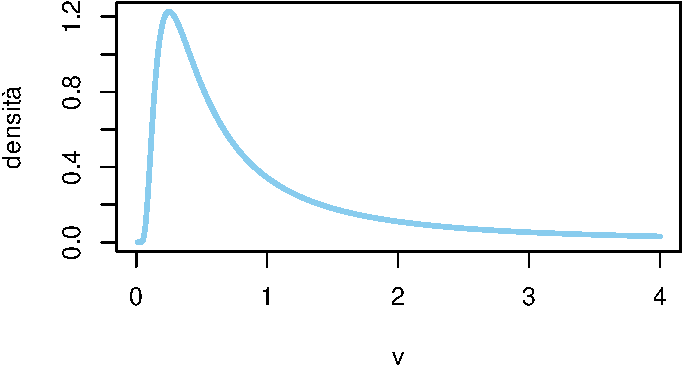
\includegraphics[keepaspectratio]{05-VA_gaussiane_files/figure-pdf/unnamed-chunk-13-1.pdf}}

}

\caption{grafico della densità esponenziale inversa con \(v_0=1\)}

\end{figure}%

Con questa scelta, avendo osservato \(X=x\), la formula di Bayes implica
che la densità per \(V\) è
\[ \begin{split} p(V=v| X=x) & \propto p(V=v|\Omega ) p(X =x | M=m_0, V=v) \\
& \propto \exp\bra{ - \frac{v_0}{2v} } \frac 1 {v^2} \exp\bra{-\frac 1 {2v}  (x-m_0)^2 } \frac{1}{\sqrt{v}}\\
&\propto\exp\bra{ - \frac{ \bra{v_0 + (x-m_0)^2} } {2v}} \frac{1}{v^{5/2}}\end{split}\]
Si tratta di una densità continua molto simile a quella a priori, in cui
il nuovo parametro (al posto di \(v_0\)) è
\[ v_{|X=x} = v_0 + (x-m_0)^2.\] A prima vista potrebbe quindi sembrare
che la varianza cresca sempre, ma bisogna anche notare che il termine
\(v^2\) al denominatore è sostituito con \(v^{5/2}\). Questo ha
l'effetto di trasformare la densità circa in modo che, se \((x-m_0)^2\)
è minore di \(v_0\), allora la densità di \(V\) si concentra verso
valori più vicini a \(0\), viceversa se \((x-m_0)^2\) è maggiore, allora
la densità di \(V\) si concentra verso valori maggiori.

\begin{Shaded}
\begin{Highlighting}[]
\NormalTok{deltav}\OtherTok{=}\FloatTok{0.01}
\NormalTok{v}\OtherTok{=}\FunctionTok{seq}\NormalTok{(deltav, }\DecValTok{4}\NormalTok{, }\AttributeTok{by=}\NormalTok{deltav)}

\CommentTok{\# densità a priori}

\NormalTok{v\_0 }\OtherTok{=} \DecValTok{1}
\NormalTok{densita\_esp\_inv }\OtherTok{=} \FunctionTok{exp}\NormalTok{(}\SpecialCharTok{{-}}\NormalTok{(v\_0}\SpecialCharTok{/}\NormalTok{(}\DecValTok{2}\SpecialCharTok{*}\NormalTok{v)))}\SpecialCharTok{/}\NormalTok{v}\SpecialCharTok{\^{}}\DecValTok{2}
\NormalTok{densita\_esp\_inv }\OtherTok{=}\NormalTok{ densita\_esp\_inv}\SpecialCharTok{/}\FunctionTok{sum}\NormalTok{(densita\_esp\_inv }\SpecialCharTok{*}\NormalTok{deltav)}


\CommentTok{\# parametro m\_0 e osservazione di X}
\NormalTok{m\_0 }\OtherTok{=} \DecValTok{0}
\NormalTok{x\_1}\OtherTok{=}\DecValTok{0}
\NormalTok{x\_2}\OtherTok{=}\DecValTok{2}

\DocumentationTok{\#\# Usiamo direttamente la formula trovata sopra}
\NormalTok{v\_x\_1 }\OtherTok{=}\NormalTok{ v\_0 }\SpecialCharTok{+}\NormalTok{ (x\_1}\SpecialCharTok{{-}}\NormalTok{m\_0)}\SpecialCharTok{\^{}}\DecValTok{2}
\NormalTok{dens\_post\_x\_1 }\OtherTok{=} \FunctionTok{exp}\NormalTok{(}\SpecialCharTok{{-}}\NormalTok{(v\_x\_1}\SpecialCharTok{/}\NormalTok{(}\DecValTok{2}\SpecialCharTok{*}\NormalTok{v)))}\SpecialCharTok{/}\NormalTok{v}\SpecialCharTok{\^{}}\NormalTok{\{}\DecValTok{5}\SpecialCharTok{/}\DecValTok{2}\NormalTok{\}}
\NormalTok{dens\_post\_x\_1 }\OtherTok{=}\NormalTok{ dens\_post\_x\_1}\SpecialCharTok{/}\FunctionTok{sum}\NormalTok{(dens\_post\_x\_1}\SpecialCharTok{*}\NormalTok{deltav)}

\NormalTok{v\_x\_2 }\OtherTok{=}\NormalTok{ v\_0 }\SpecialCharTok{+}\NormalTok{ (x\_2}\SpecialCharTok{{-}}\NormalTok{m\_0)}\SpecialCharTok{\^{}}\DecValTok{2}
\NormalTok{dens\_post\_x\_2 }\OtherTok{=} \FunctionTok{exp}\NormalTok{(}\SpecialCharTok{{-}}\NormalTok{(v\_x\_2}\SpecialCharTok{/}\NormalTok{(}\DecValTok{2}\SpecialCharTok{*}\NormalTok{v)))}\SpecialCharTok{/}\NormalTok{v}\SpecialCharTok{\^{}}\NormalTok{\{}\DecValTok{5}\SpecialCharTok{/}\DecValTok{2}\NormalTok{\}}
\NormalTok{dens\_post\_x\_2 }\OtherTok{=}\NormalTok{ dens\_post\_x\_2}\SpecialCharTok{/}\FunctionTok{sum}\NormalTok{(dens\_post\_x\_2}\SpecialCharTok{*}\NormalTok{deltav)}

\CommentTok{\# grafico e legenda}

\FunctionTok{plot}\NormalTok{(v, densita\_esp\_inv , }\AttributeTok{type=}\StringTok{\textquotesingle{}l\textquotesingle{}}\NormalTok{, }\AttributeTok{xlab=}\StringTok{\textquotesingle{}v\textquotesingle{}}\NormalTok{, }\AttributeTok{ylab=}\StringTok{\textquotesingle{}densità\textquotesingle{}}\NormalTok{, }\AttributeTok{ylim=}\FunctionTok{c}\NormalTok{(}\DecValTok{0}\NormalTok{,}\DecValTok{2}\NormalTok{), }\AttributeTok{col=}\NormalTok{miei\_colori[}\DecValTok{1}\NormalTok{], }\AttributeTok{lwd=}\DecValTok{3}\NormalTok{)}
\FunctionTok{lines}\NormalTok{(v, dens\_post\_x\_1, }\AttributeTok{type=}\StringTok{\textquotesingle{}l\textquotesingle{}}\NormalTok{, }\AttributeTok{col=}\NormalTok{miei\_colori[}\DecValTok{2}\NormalTok{], }\AttributeTok{lwd=}\DecValTok{3}\NormalTok{)}
\FunctionTok{lines}\NormalTok{(v, dens\_post\_x\_2, }\AttributeTok{type=}\StringTok{\textquotesingle{}l\textquotesingle{}}\NormalTok{, }\AttributeTok{col=}\NormalTok{miei\_colori[}\DecValTok{3}\NormalTok{], }\AttributeTok{lwd=}\DecValTok{3}\NormalTok{)}

\CommentTok{\# Legenda}

\FunctionTok{legend}\NormalTok{(}\StringTok{\textquotesingle{}topright\textquotesingle{}}\NormalTok{, }\AttributeTok{legend=}\FunctionTok{c}\NormalTok{(}\StringTok{\textquotesingle{}a priori\textquotesingle{}}\NormalTok{,}\StringTok{\textquotesingle{}X=0\textquotesingle{}}\NormalTok{, }\StringTok{\textquotesingle{}X=2\textquotesingle{}}\NormalTok{), }\AttributeTok{fill=}\NormalTok{miei\_colori[}\DecValTok{1}\SpecialCharTok{:}\DecValTok{3}\NormalTok{])}
\end{Highlighting}
\end{Shaded}

\begin{figure}[H]

{\centering \pandocbounded{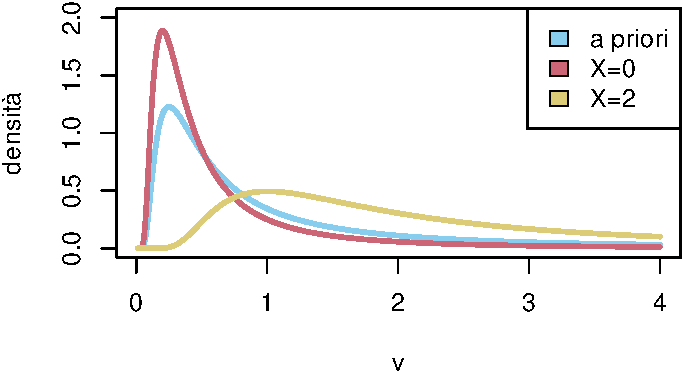
\includegraphics[keepaspectratio]{05-VA_gaussiane_files/figure-pdf/unnamed-chunk-14-1.pdf}}

}

\caption{grafico della densità a priori per \(V\), con parametri
\(v_0=1\), \(m_0=0\), e della densità avendo osservato \(X=0\) (in
rosso) oppure \(X=2\) (in blu)}

\end{figure}%

Lo studio del caso generale dal punto di vista bayesiano, ossia della
variabile congiunta \((M,V)\) (senza supporre che una sia costante nota
a priori), è più complicato analiticamente. Tuttavia possiamo renderci
conto di come l'informazione a priori sia rilevante osservando un
risultato numerico ottenuto assumendo che \(M\) e \(V\) siano a priori
indipendenti, la prima uniformemente distribuita su \([2,4]\), la
seconda sull'intervallo \([1, 3]\), e si osserva \(X=1\). La stima di
massima verosimiglianza (calcolata in precedenza su tutti i valori di
\(m\) e \(v\) sulla stessa osservazione \(X=1\)) era \(m_{{\mle}}=1\),
\(v_{{\mle}} = 0\), ora l'informazione a priori induce una densità
congiunta (le cui marginali non sono indipendenti) con un punto di
massimo in \(m=2\), \(v=3\). Possiamo intepretare parzialmente questo
fatto notando che essendo media a priori tra \(2\) e \(4\),
l'osservazione \(X=1\) sposta la media verso il valore più basso
possibile \(m=2\).

\begin{Shaded}
\begin{Highlighting}[]
\NormalTok{deltam}\OtherTok{=}\FloatTok{0.1}
\NormalTok{deltav}\OtherTok{=}\FloatTok{0.05}

\NormalTok{m}\OtherTok{=} \FunctionTok{seq}\NormalTok{(}\DecValTok{2}\NormalTok{,}\DecValTok{4}\NormalTok{, }\AttributeTok{by=}\NormalTok{deltam)}
\NormalTok{v}\OtherTok{=}\FunctionTok{seq}\NormalTok{(}\DecValTok{1}\NormalTok{, }\DecValTok{3}\NormalTok{, }\AttributeTok{by=}\NormalTok{deltav)}

\NormalTok{N\_m }\OtherTok{=} \FunctionTok{length}\NormalTok{(m)}
\NormalTok{N\_v }\OtherTok{=} \FunctionTok{length}\NormalTok{(v)}

\CommentTok{\# osservazione}

\NormalTok{x}\OtherTok{=}\DecValTok{0}


\CommentTok{\# creiamo una matrice con i valori della verosimiglianza}

\NormalTok{L }\OtherTok{=} \FunctionTok{matrix}\NormalTok{( }\DecValTok{0}\NormalTok{, }\AttributeTok{nrow =}\NormalTok{ N\_m, }\AttributeTok{ncol =}\NormalTok{N\_v)}

\ControlFlowTok{for}\NormalTok{ (i }\ControlFlowTok{in} \DecValTok{1}\SpecialCharTok{:}\NormalTok{N\_m)\{}
  \ControlFlowTok{for}\NormalTok{ (j }\ControlFlowTok{in} \DecValTok{1}\SpecialCharTok{:}\NormalTok{N\_v)\{}
\NormalTok{    L[i,j]}\OtherTok{=} \FunctionTok{exp}\NormalTok{(}\SpecialCharTok{{-}}\NormalTok{(m[i]}\SpecialCharTok{{-}}\NormalTok{x)}\SpecialCharTok{\^{}}\DecValTok{2}\SpecialCharTok{/}\NormalTok{(}\DecValTok{2}\SpecialCharTok{*}\NormalTok{v[j])) }\SpecialCharTok{/} \FunctionTok{sqrt}\NormalTok{(}\DecValTok{2} \SpecialCharTok{*}\NormalTok{pi }\SpecialCharTok{*}\NormalTok{v[j])}
\NormalTok{  \}}
\NormalTok{\}}

\NormalTok{posteriori }\OtherTok{=}\NormalTok{ L}\SpecialCharTok{/}\FunctionTok{sum}\NormalTok{(L }\SpecialCharTok{*}\NormalTok{deltam }\SpecialCharTok{*}\NormalTok{deltav)}


\CommentTok{\# usiamo filled.contour() per produrre il grafico e la scala di valori accanto}

\FunctionTok{filled.contour}\NormalTok{(m, v, posteriori, }\AttributeTok{color.palette=}\NormalTok{viridis, }\AttributeTok{xlab=}\StringTok{\textquotesingle{}m\textquotesingle{}}\NormalTok{, }\AttributeTok{ylab=}\StringTok{\textquotesingle{}v\textquotesingle{}}\NormalTok{)}
\end{Highlighting}
\end{Shaded}

\begin{center}
\pandocbounded{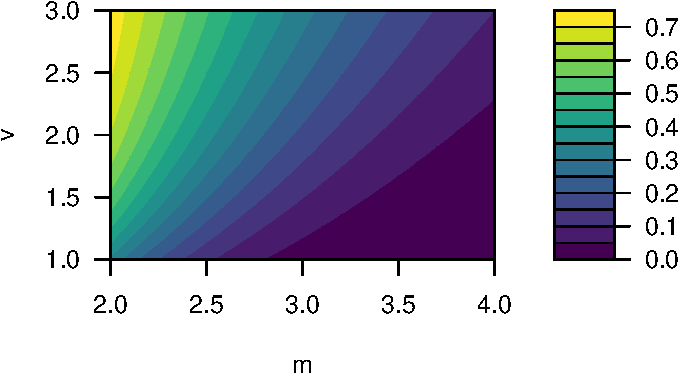
\includegraphics[keepaspectratio]{05-VA_gaussiane_files/figure-pdf/unnamed-chunk-15-1.pdf}}
\end{center}

\section{Stima dei parametri da osservazioni
indipendenti}\label{sec-stimaindipendenti}

In questa sezione estendiamo i risultati della precedente al caso in cui
osservano variabili indipendenti \((X_i)_{i=1}^n\), tutte gaussiane con
i medesimi parametri (il termine statistico è un \emph{campione} di
taglia \(n\), il numero di osservazioni). Per avvicinare la notazione al
caso precedente, si può alternativamente descrivere la situazione
dicendo che il robot stima i parametri sulla base dell'osservazione di
un (singolo) vettore aleatorio gaussiano \(X = (X_i)_{i=1}^n\) a valori
in \(\R^n\). Nella sezione successiva indichiamo come estendere al caso
di \(n\) osservazioni indipendenti di variabili gaussiane a loro volta
vettoriali.

La situazione che stiamo descrivendo è molto comune, ad esempio se
ciascuna \(X_i\) rappresenta una misura della stessa quantità
(rappresentata dal parametro di media) affetta da una imprecisione (un
``rumore'') di una opportuna intensità (la deviazione standard):
sfruttando l'indipendenza risulta che l'effetto del rumore è mitigato e
si ottiene una stima più precisa.

Introduciamo quindi la seguente notazione analoga a quella della sezione
precedente: i parametri di cascuna \(X_i\), ossia la media \(\E{X_i}\) e
la varianza \(\Var{X_i}\) non dipendono da \(i\), e scriviamo quindi
\[ m = \E{X_i} \quad v = \Var{X_i} \quad \text{per ogni $i=1, \ldots, n$.}\]
Come nel caso della singola osservazione, si introducono le rispettive
variabili aleatorie \(M\) per la media, \(V\) per la varianza (la
seconda a valori positivi).

La rete bayesiana associata è rappresentata in figura e generalizza
quella della sezione precedente (abbiamo introdotto la variabile
congiunta \((M,V)\) per semplificare la notazione).

\begin{figure}[H]

{\centering \pandocbounded{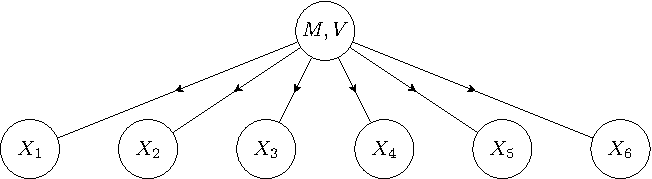
\includegraphics[keepaspectratio]{05-VA_gaussiane_files/figure-pdf/unnamed-chunk-16-1.pdf}}

}

\caption{Rete bayesiana tra le variabili \((M,V)\) e le
\((X_i)_{i=1}^n\) per \(n=6\)}

\end{figure}%

Poter disporre di più osservazioni indipendenti degli stessi parametri
intuitivamente permette di ottenere stime più precise, un fatto che ora
vediamo sia tramite l'approccio di massima verosimiglianza che quello
bayesiano.

\subsection{Stima di massima
verosimiglianza}\label{stima-di-massima-verosimiglianza-1}

L'ipotesi di indipendenza, noti \(m\) e \(v\), si traduce nel fatto che
la densità dell'osservazione di \(X=x\), ossia la congiunta delle
osservazioni \(X_i=x_i\) per \(i=1,\ldots, n\), è la verosimiglianza
\[ \begin{split} L(m, v; x)& = p(X=x|M=m,V=v)  = p(X_1 = x_1, \ldots X_n = x_n | m, v) \\
& =  p(X_1 = x_1 | m,v) \cdot \ldots \cdot p(X_n = x_n | m, v) \\
& = \prod_{i=1}^n \exp\bra{ -\frac{1}{2v} (x_i -m)^2 } \frac{1}{\sqrt{ 2 \pi v}} \\
& \propto \exp\bra{ - \frac {n}{2} \bra{ \frac 1 {nv} \sum_{i=1}^n (x_i - m)^2 +  \log( v )}},\end{split}\]
dove nell'ultimo passaggio abbiamo omesso la costante moltiplicativa
\((2 \pi)^{n/2}\) (per semplificare la notazione).

\begin{Shaded}
\begin{Highlighting}[]
\NormalTok{deltam}\OtherTok{=}\FloatTok{0.1}
\NormalTok{deltav}\OtherTok{=}\FloatTok{0.05}

\NormalTok{m}\OtherTok{=} \FunctionTok{seq}\NormalTok{(}\DecValTok{0}\NormalTok{,}\DecValTok{2}\NormalTok{, }\AttributeTok{by=}\NormalTok{deltam)}
\NormalTok{v}\OtherTok{=}\FunctionTok{seq}\NormalTok{(}\FloatTok{0.01}\NormalTok{,}\DecValTok{1}\NormalTok{, }\AttributeTok{by=}\NormalTok{deltav)}

\NormalTok{N\_m }\OtherTok{=} \FunctionTok{length}\NormalTok{(m)}
\NormalTok{N\_v }\OtherTok{=} \FunctionTok{length}\NormalTok{(v)}

\CommentTok{\# osservazioni}

\NormalTok{x}\OtherTok{=}\FunctionTok{c}\NormalTok{(}\DecValTok{1}\NormalTok{,}\DecValTok{2}\NormalTok{,}\FloatTok{1.5}\NormalTok{,}\FloatTok{0.5}\NormalTok{)}
\NormalTok{n}\OtherTok{=} \FunctionTok{length}\NormalTok{(x)}


\CommentTok{\# creiamo una matrice con i valori della verosimiglianza}

\NormalTok{L }\OtherTok{=} \FunctionTok{matrix}\NormalTok{( }\DecValTok{1}\NormalTok{, }\AttributeTok{nrow =}\NormalTok{ N\_m, }\AttributeTok{ncol =}\NormalTok{N\_v)}

\ControlFlowTok{for}\NormalTok{ (i }\ControlFlowTok{in} \DecValTok{1}\SpecialCharTok{:}\NormalTok{N\_m)\{}
  \ControlFlowTok{for}\NormalTok{ (j }\ControlFlowTok{in} \DecValTok{1}\SpecialCharTok{:}\NormalTok{N\_v)\{}
    \ControlFlowTok{for}\NormalTok{ (obs }\ControlFlowTok{in}\NormalTok{ x)\{}
\NormalTok{      L[i,j]}\OtherTok{=}\NormalTok{ L[i,j]}\SpecialCharTok{*}\FunctionTok{exp}\NormalTok{(}\SpecialCharTok{{-}}\NormalTok{(m[i]}\SpecialCharTok{{-}}\NormalTok{obs)}\SpecialCharTok{\^{}}\DecValTok{2}\SpecialCharTok{/}\NormalTok{(}\DecValTok{2}\SpecialCharTok{*}\NormalTok{v[j])) }\SpecialCharTok{/} \FunctionTok{sqrt}\NormalTok{(}\DecValTok{2} \SpecialCharTok{*}\NormalTok{pi }\SpecialCharTok{*}\NormalTok{v[j])}
\NormalTok{    \}}
\NormalTok{  \}}
\NormalTok{\}}

\CommentTok{\# usiamo stavolta filled.contour() per produrre il grafico e la scala di valori accanto}

\FunctionTok{filled.contour}\NormalTok{(m, v, L, }\AttributeTok{color.palette=}\NormalTok{viridis, }\AttributeTok{xlab=}\StringTok{\textquotesingle{}m\textquotesingle{}}\NormalTok{, }\AttributeTok{ylab=}\StringTok{\textquotesingle{}v\textquotesingle{}}\NormalTok{)}
\end{Highlighting}
\end{Shaded}

\begin{figure}[H]

{\centering \pandocbounded{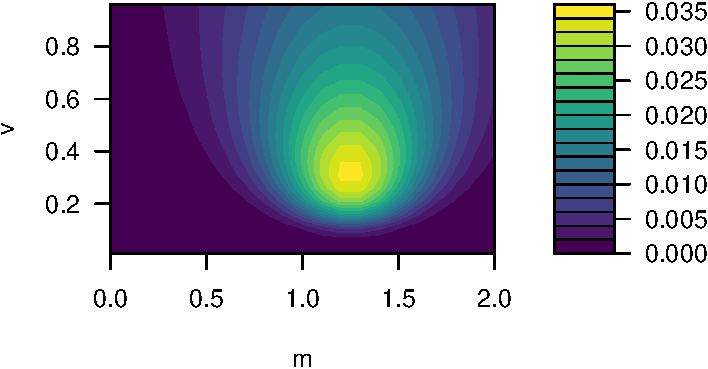
\includegraphics[keepaspectratio]{05-VA_gaussiane_files/figure-pdf/unnamed-chunk-17-1.pdf}}

}

\caption{verosimiglianza per \(m\) e \(v\), associata alle osservazioni
\(x = (1, 2, 1.5, 0.5)\).}

\end{figure}%

Dal grafico sopra vediamo che la verosimiglianza è una funzione più
interessante del caso di una singola osservazione e in particolare il
massimo non è necessariamente per \(v=0\). Per applicare il metodo di
massima verosimiglianza, passando al logaritmo e moltiplicando per
\(-2/n\) e tralasciando costanti additive (che non hanno nessun ruolo
utile nella procedura) si tratta quindi di determinare \(m_{{\mle}}\) e
\(v_{{\mle}}\) che \emph{minimizzano} la funzione
\[ (m, v) \mapsto  \frac{1}{v} \sqa{ \frac 1 {n} \sum_{i=1}^n (x_i - m)^2} +  \log( v ) \]
Ragionando come nel caso della singola osservazione, deriviamo rispetto
ad \(m\) (fissato \(v\)) e imponiamo che la derivata si annulli. Si
trova la condizione
\[  2 \sum_{i=1}^n (x_i - m) = 0 \quad \text{da cui} \quad m = \frac{1}{n} \sum_{i=1}^n x_i \]
è la media aritmetica delle osservazioni (detta anche \textbf{media
empirica} o campionaria, in inglese \emph{sample mean}), e indicata
anche brevemente con \[ \bar{x} = \frac{1}{n} \sum_{i=1}^n x_i,\] Mentre
se deriviamo rispetto a \(v\), tenendo fisso \(m\), si trova
analogamente al caso della singola osservazione che
\[  -\frac 1 { v^2}  \frac 1 n \sum_{i=1}^n(x_i-m)^2 + \frac{1}{v} = 0, \quad \text{da cui} \quad  v = \frac 1 n \sum_{i=1}^n (x_i-m)^2.\]
dovendo massimizzare la funzione delle due variabili si trova quindi la
coppia
\[ m_{{\mle}} =\bar{x} = \frac 1 n \sum_{i=1}^n x_i \quad v_{{\mle}} = \frac{1}{n}\sum_{i=1}^n(x_i-\bar{x})^2,\]
dove l'ultima quantità è detta anche \textbf{varianza campionaria}
(\emph{sample variance} in inglese). Volendo specificare, questa è la
versione detta anche
\emph{distorta}\footnote{Il termine ha un significato tecnico preciso in statistica, purtroppo la scelta è infelice perché porta con sé una sfumatura dispregiativa, quando non è necessariamente il caso}
(in inglese \emph{biased}) della varianza campionaria, dove la versione
``corretta'' o meglio \emph{non distorta} (\emph{unbiased}) contiene
invece il fattore \(n-1\) a denominatore, una differenza minima quando
\(n\) è grande, sulle cui ragioni non ci soffermiamo -- tuttavia va
tenuto presente che molte funzioni in R usano appunto la versione non
distorta.

Come nel caso della singola osservazione, i calcoli sopra ci mostrano
anche che, 1. se il pararametro di varianza \(V=v_0 >0\) è noto (ossia
\(V=v_0\) è costante), la stima di massima verosimiglianza per il
parametro di media è \(m_{{\mle}}  = \bar{x}\) (qualsiasi sia \(v_0\)),
2. se il parametro di media \(M=m_0\in \R\) è noto (ossia \(M=m_0\) è
costante rispetto all'informazione a priori), allora la stima di massima
verosimiglianza per il parametro di varianza è
\[ v_{{\mle}} = \frac 1 n \sum_{i=1}(x_i-m_0)^2.\]

Consideriamo il classico dataset ``iris''\footnote{\url{https://en.wikipedia.org/wiki/Iris_flower_data_set}}
che contiene \(150\) osservazioni di esemplari diversi da \(3\) specie
della pianta Iris appunto. Non è necessario importarlo in R perché è
sempre disponibile (nella libreria \texttt{datasets} precaricata vi sono
alcune raccolte di dati che si usano frequentemente come esempi). Con la
funzione \texttt{head()}, possiamo visualizzare alcuni dati per farci
una idea generale. L'output del comando \texttt{head(iris)} è presentato
sotto.

\begin{longtable}[]{@{}rrrrl@{}}
\caption{Le prime 10 righe del dataset Iris.}\tabularnewline
\toprule\noalign{}
Sepal.Length & Sepal.Width & Petal.Length & Petal.Width & Species \\
\midrule\noalign{}
\endfirsthead
\toprule\noalign{}
Sepal.Length & Sepal.Width & Petal.Length & Petal.Width & Species \\
\midrule\noalign{}
\endhead
\bottomrule\noalign{}
\endlastfoot
5.1 & 3.5 & 1.4 & 0.2 & setosa \\
4.9 & 3.0 & 1.4 & 0.2 & setosa \\
4.7 & 3.2 & 1.3 & 0.2 & setosa \\
4.6 & 3.1 & 1.5 & 0.2 & setosa \\
5.0 & 3.6 & 1.4 & 0.2 & setosa \\
5.4 & 3.9 & 1.7 & 0.4 & setosa \\
4.6 & 3.4 & 1.4 & 0.3 & setosa \\
5.0 & 3.4 & 1.5 & 0.2 & setosa \\
4.4 & 2.9 & 1.4 & 0.2 & setosa \\
4.9 & 3.1 & 1.5 & 0.1 & setosa \\
\end{longtable}

Per calcolare media e varianza campionaria delle osservazioni della
variabile ``lunghezza del sepalo'' (una parte del fiore), è sufficiente
usare le funzioni \texttt{mean()} e \texttt{var()}.

\begin{Shaded}
\begin{Highlighting}[]
\FunctionTok{mean}\NormalTok{(iris}\SpecialCharTok{$}\NormalTok{Sepal.Length)}
\end{Highlighting}
\end{Shaded}

\begin{verbatim}
[1] 5.843333
\end{verbatim}

\begin{Shaded}
\begin{Highlighting}[]
\FunctionTok{var}\NormalTok{(iris}\SpecialCharTok{$}\NormalTok{Sepal.Length)}
\end{Highlighting}
\end{Shaded}

\begin{verbatim}
[1] 0.6856935
\end{verbatim}

Per calcolare direttamente la deviazione standard dal campione, ossia la
radice quadrata dela varianza campionaria, si può usare \texttt{sd()}.

\begin{Shaded}
\begin{Highlighting}[]
\FunctionTok{sd}\NormalTok{(iris}\SpecialCharTok{$}\NormalTok{Sepal.Length)}
\end{Highlighting}
\end{Shaded}

\begin{verbatim}
[1] 0.8280661
\end{verbatim}

Anche prima di calcolare media e varianza, è sempre buona pratica
rappresentare graficamente i dati, in questo caso ad esempio tramite un
istogramma.

\begin{Shaded}
\begin{Highlighting}[]
\FunctionTok{hist}\NormalTok{(iris}\SpecialCharTok{$}\NormalTok{Sepal.Length, }\AttributeTok{breaks =} \DecValTok{10}\NormalTok{, }\AttributeTok{xlab=}\StringTok{"Lughezza dei sepali"}\NormalTok{, }\AttributeTok{ylab =} \StringTok{"Frequenza"}\NormalTok{, }\AttributeTok{main=}\StringTok{""}\NormalTok{, }\AttributeTok{col=}\NormalTok{miei\_colori[}\DecValTok{1}\NormalTok{])}
\end{Highlighting}
\end{Shaded}

\begin{figure}[H]

{\centering \pandocbounded{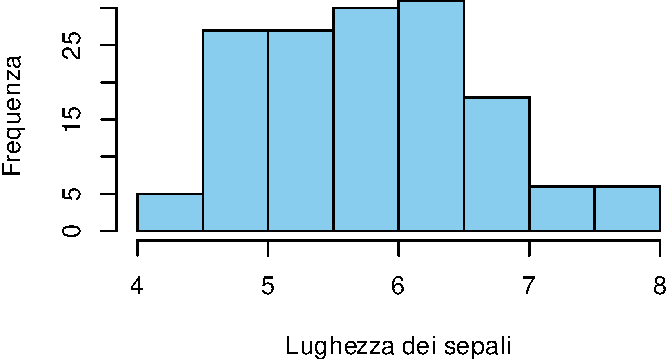
\includegraphics[keepaspectratio]{05-VA_gaussiane_files/figure-pdf/unnamed-chunk-21-1.pdf}}

}

\caption{Istogramma della lunghezza dei sepali osservata nel dataset
Iris}

\end{figure}%

\subsection{Stima bayesiana della media, varianza
nota}\label{stima-bayesiana-della-media-varianza-nota}

Vediamo ora l'approccio bayesiano, applicandolo prima alla stima della
media, supponendo che la varianza \(V = v_0\) sia nota (e quindi
costante rispetto all'informazione a priori). Come nel caso della
singola osservazione, per avere dei calcoli trattabili analiticamente,
conviene supporre che \(M\) a priori abbia una densità gaussiana di
parametri \(\mathcal{N}(m_0, \sigma_m^2)\), e avendo osservato
\(X=x= (x_i)_{i=1}^n\), il robot calcola poi la densità di \(M\) tramite
la formula di Bayes
\[ \begin{split} p(M=m| X=x) & \propto p(M=m|\Omega ) p(X=x | M=m, V=v_0) \\
& \propto \exp\bra{ -\frac 1 2 \bra{ \frac{ (m-m_0)^2}{\sigma_m^2} + \sum_{i=1}^n \frac { (x_i-m)^2}{v_0} }}.\end{split}\]
Si trova quindi, come nel caso \(n=1\), una nuova densità gaussiana, di
cui con passaggi elementari si ricavano i parametri di media e varianza
(che dipendono naturalmente dall'osservazione \(X=x\))
\[ m_{|X=x} = (1-\alpha) \bar{x} + \alpha m_0, \quad \sigma^2_{m|X=x} = \sigma_m^2\alpha,\]
dove abbiamo posto \[\alpha = \frac{1}{1+n\sigma_m^2/v_0 } \in (0,1).\]
Come nel caso della singola osservazione, la nuova informazione \(X=x\),
ossia \(X_i=x_i\) per \(i=1, \ldots, n\), sposta la fiducia del robot
verso la media campionaria \(\bar{x}\), ossia la stima di massima
verosimiglianza.

\begin{remark}
È naturale chiedersi cosa accada per \(n\) grande, in particolare se
\(n >> v_0/\sigma_m^2\). In tal caso, si ha che \(\alpha\) tende a \(0\)
e quindi il parametro di media della \(M\) a posteriori tende alla media
campionaria \(\bar{x}\), ossia la stima di massima verosimiglianza. Per
lo stesso motivo, anche che la varianza di \(M\) tende a \(0\), per cui
la distribuzione di \(M\) si concentra sempre più intorno al valore
\(\bar{x}\). Questo è un caso particolare di un teorema molto più
generale, noto come \emph{legge dei grandi numeri}, il quale afferma che
la differenza tra la media campionaria di un gran numero di variabili
aleatorie indipendenti tra loro (tutte con lo stesso valor medio e
varianza) e il valor medio teorico diventa piccola con grandissima
probabilità al tendere della numerosità del campione \(n\) all'infinito.
Ritorneremo su questo fatto nella Sezione Sezione~\ref{sec-lln}.
\end{remark}

\subsection{Stima bayesiana della varianza, valor medio
noto}\label{stima-bayesiana-della-varianza-valor-medio-noto}

Supponiamo ora che \(M =m_0\) sia costante (rispetto all'informazione
nota prima di osservare \(X=x\)) e introduciamo come nella sezione
precedente una densità a priori per \(V\) di tipo \emph{esponenziale
inversa}, dove \(v_0>0\) è un parametro noto:
\[ p( V = v|\Omega)  \propto p(1/V = 1/v)\frac{1}{v^2} \propto \exp\bra{ -\frac{v_0}{2v}}\frac{1}{v^2}.\]

Usando la formula di Bayes,
\[ \begin{split} p(V=v| X=x) & \propto p(V=v|\Omega ) p(X =x | M=m_0, V=v) \\
& \propto \exp\bra{ - \frac{v_0}{2v} } \frac 1 {v^2} \exp\bra{ - \frac{1}{v} \sum_{i=1}^n (x_i-m_0)^2} \frac{1}{v^{n/2}}\\
&\propto\exp\bra{ - \frac{ \bra{v_0 + \sum_{i=1}^n (x_i-m_0)^2} } {2v}} \frac{1}{v^{(4+n)/2}}.\end{split}\]
Come nel caso della singola osservazione, si tratta di una densità
continua molto simile a quella a priori, in cui il nuovo parametro (al
posto di \(v_0\)) è \[ v_{|X=x} = v_0 + \sum_{i=1}^n (x_i-m_0)^2,\] ma
vi è anche il termine \(v^{(4+n)/2}\) a denominatore, che sempre più
rilevante al crescere di \(n\). Infatti, il punto di massimo della
densità a posteriori (che possiamo ottenere passando al logaritmo, e
imponendo la derivata nulla) è dato dall'espressione
\[ \frac{ v_{|X=x}}{4+n} =  \frac{ v_0 + \sum_{i=1}^n (x_i-m_0)^2}{4+n }\]
che al crescere di \(n\) è asintoticamente equivalente alla stima di
massima verosimiglianza
\[v_{{\mle}} = \frac{1}{n} \sum_{i=1}^n (x_i-m_0)^2\] (supponendo la
media \(m_0\) nota).

\begin{Shaded}
\begin{Highlighting}[]
\NormalTok{deltav}\OtherTok{=}\FloatTok{0.01}
\NormalTok{v}\OtherTok{=}\FunctionTok{seq}\NormalTok{(deltav, }\DecValTok{4}\NormalTok{, }\AttributeTok{by=}\NormalTok{deltav)}

\CommentTok{\# densità a priori}

\NormalTok{v\_0 }\OtherTok{=} \DecValTok{1}
\NormalTok{densita\_esp\_inv }\OtherTok{=} \FunctionTok{exp}\NormalTok{(}\SpecialCharTok{{-}}\NormalTok{(v\_0}\SpecialCharTok{/}\NormalTok{(}\DecValTok{2}\SpecialCharTok{*}\NormalTok{v)))}\SpecialCharTok{/}\NormalTok{v}\SpecialCharTok{\^{}}\DecValTok{2}
\NormalTok{densita\_esp\_inv }\OtherTok{=}\NormalTok{ densita\_esp\_inv}\SpecialCharTok{/}\FunctionTok{sum}\NormalTok{(densita\_esp\_inv }\SpecialCharTok{*}\NormalTok{deltav)}


\CommentTok{\# parametro m\_0 e osservazione di X}
\NormalTok{m\_0 }\OtherTok{=} \DecValTok{0}
\NormalTok{x }\OtherTok{=} \FunctionTok{c}\NormalTok{(}\DecValTok{1}\NormalTok{,}\DecValTok{2}\NormalTok{,}\FloatTok{1.5}\NormalTok{,}\FloatTok{0.5}\NormalTok{)}
\NormalTok{n }\OtherTok{=} \FunctionTok{length}\NormalTok{(x)}

\CommentTok{\# Usiamo la formula trovata per la densità a posteriori}
\NormalTok{v\_x }\OtherTok{=}\NormalTok{ v\_0 }\SpecialCharTok{+} \FunctionTok{sum}\NormalTok{( (x}\SpecialCharTok{{-}}\NormalTok{m\_0)}\SpecialCharTok{\^{}}\DecValTok{2}\NormalTok{)}
\NormalTok{dens\_post\_x }\OtherTok{=} \FunctionTok{exp}\NormalTok{(}\SpecialCharTok{{-}}\NormalTok{(v\_x}\SpecialCharTok{/}\NormalTok{(}\DecValTok{2}\SpecialCharTok{*}\NormalTok{v)))}\SpecialCharTok{/}\NormalTok{v}\SpecialCharTok{\^{}}\NormalTok{((}\DecValTok{4}\SpecialCharTok{+}\NormalTok{n)}\SpecialCharTok{/}\DecValTok{2}\NormalTok{)}
\NormalTok{dens\_post\_x }\OtherTok{=}\NormalTok{ dens\_post\_x}\SpecialCharTok{/}\FunctionTok{sum}\NormalTok{(dens\_post\_x}\SpecialCharTok{*}\NormalTok{deltav)}

\CommentTok{\# grafico e legenda}

\FunctionTok{plot}\NormalTok{(v, densita\_esp\_inv , }\AttributeTok{type=}\StringTok{\textquotesingle{}l\textquotesingle{}}\NormalTok{, }\AttributeTok{xlab=}\StringTok{\textquotesingle{}v\textquotesingle{}}\NormalTok{, }\AttributeTok{ylab=}\StringTok{\textquotesingle{}densità\textquotesingle{}}\NormalTok{, }\AttributeTok{ylim=}\FunctionTok{c}\NormalTok{(}\DecValTok{0}\NormalTok{,}\FloatTok{1.5}\NormalTok{),}\AttributeTok{col=}\NormalTok{miei\_colori[}\DecValTok{1}\NormalTok{], }\AttributeTok{lwd=}\DecValTok{3}\NormalTok{)}
\FunctionTok{lines}\NormalTok{(v, dens\_post\_x, }\AttributeTok{type=}\StringTok{\textquotesingle{}l\textquotesingle{}}\NormalTok{, }\AttributeTok{col=}\NormalTok{miei\_colori[}\DecValTok{2}\NormalTok{], }\AttributeTok{lwd=}\DecValTok{3}\NormalTok{)}



\CommentTok{\# Legenda}

\FunctionTok{legend}\NormalTok{(}\StringTok{\textquotesingle{}topright\textquotesingle{}}\NormalTok{, }\AttributeTok{legend=}\FunctionTok{c}\NormalTok{(}\StringTok{\textquotesingle{}a priori\textquotesingle{}}\NormalTok{,}\StringTok{\textquotesingle{}a posteriori\textquotesingle{}}\NormalTok{), }\AttributeTok{fill=}\NormalTok{miei\_colori[}\DecValTok{1}\SpecialCharTok{:}\DecValTok{2}\NormalTok{])}
\end{Highlighting}
\end{Shaded}

\begin{figure}[H]

{\centering \pandocbounded{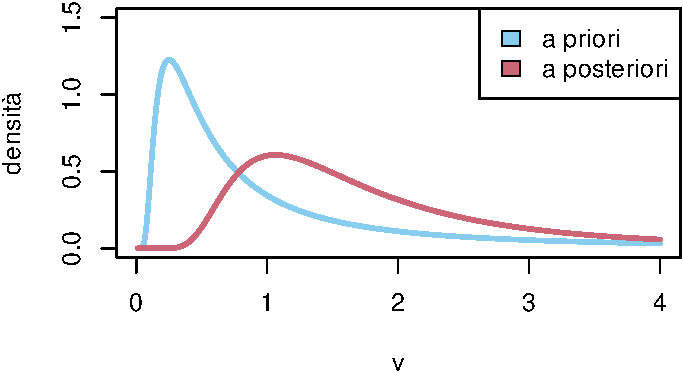
\includegraphics[keepaspectratio]{05-VA_gaussiane_files/figure-pdf/unnamed-chunk-22-1.pdf}}

}

\caption{grafico della densità a priori per \(V\), con parametri
\(v_0=1\), \(m_0=0\), e della densità avendo osservato \$ x=(1, 2, 1.5,
0.5)\$ (la stima di massima verosimiglianza è in questo caso
\(v_{\mle} = 1\))}

\end{figure}%

\subsection{Esercizi}\label{esercizi-27}

Stimare tramite massima verosimiglianza (e mediante opportuni comandi R)
i parametri di media e deviazione standard per la lunghezza dei petali
nel dataset Iris.

Supponiamo di essere dei biologi che hanno già classificato la specie
Iris ``setosa'' e determinato che la lunghezza di un petalo è
\(1.6 \pm 0.2\). Usando i nuovi dati raccolti sulla specie (sono le
prime 50 entrate del dataset), rendere più precisa la stima della media
tramite l'approccio bayesiano (supporre che
\(\sigma_m^2  = v^2 = (0.2)^2\) sia nota).

\section{Stime nel caso vettoriale}\label{sec-stimavettoriali}

I risultati della sezione precedente si possono estendere al caso
vettoriale, ossia di \(n\) osservazioni di variabili aleatorie \(X_1\),
\ldots, \(X_n \in \R^d\), tutte indipendenti tra loro e ciascuna con
densità gaussiana vettoriale di parametri comuni
\(\mathcal{N}(m, \Sigma)\). Posta per brevità
\(X = (X_1, \ldots, X_n) \in \R^{nd}\), funzione di verosimiglianza dei
parametri di media e varianza associata all'osservazione di
\(X=x = (x_i)_{i=1}^n\), si scrive, a meno di costanti moltiplicative,
\[ L(m,\Sigma; x) \propto \exp\bra{ - \frac 1 2 \sum_{i=1}^n (x_i-m)\cdot \Sigma^{-1} (x_i-m)} \frac{1}{\bra{ \det \Sigma}^{n/2}}.\]

I calcoli analitici, già nel caso della stima di massima
verosimiglianza, sono meno agevoli e ne riportiamo solamente il
risultato. Precisamente, 1. se la varianza \(\Sigma = \Sigma_0\) è nota
(rispetto all'informazione prima di osservare le \(X_i\)), la stima di
massima verosimiglianza per il parametro di media è la media campionaria
\[ m_{{\mle}} = \bar{x} = \frac{1}{n} \sum_{i=1}^n x_i\] (qualsiasi sia
\(\Sigma_0\)).

\begin{enumerate}
\def\labelenumi{\arabic{enumi}.}
\setcounter{enumi}{1}
\tightlist
\item
  se il parametro di media \(m = m_0\in \R^d\) è noto (rispetto
  all'informazione a priori), allora la stima di massima verosimiglianza
  per la covarianza è
  \[ \Sigma_{{\mle}} = \frac 1 n \sum_{i=1}^n(x_i-m_0)(x_i-m_0)^T,\]
  dove \(T\) indica l'operazione di trasposizione (quindi il prodotto
  righe per colonne risulta in una matrice \(d\times d\)); più
  esplicitamente, la stima della covarianza tra la componente \(j\) e
  \(k\) è
  \[ (\Sigma_{{\mle}})_{jk} = \frac 1 n \sum_{i=1}^n(x_i-m_0)_j (x_i-m_0)_k.\]
  Mettendo insieme i due risultati sopra, si ottiene analogamente al
  caso reale che la stima (congiunta) di massima verosimiglianza per
  \((m,\Sigma)\) è data dalla media e dalla covarianza campionarie:
  \[ m_{{\mle}} = \bar{x} = \frac{1}{n} \sum_{i=1}^n x_i,  \quad \Sigma_{{\mle}} = \frac 1 n \sum_{i=1}^n(x_i-\bar{x})(x_i-\bar{x})^T.\]
  Osserviamo che \(\Sigma_{\mle}\) è una matrice simmetrica e
  semi-definita positiva. La si può anche interpretare come la matrice
  di covarianza della variabile aleatoria vettoriale che sceglie uno
  degli \(n\) valori osservati con probabilità uniforme discreta.
\end{enumerate}

Torniamo al dataset Iris e usiamo le funzioni \texttt{summary()} e
\texttt{cov()} per calcolare la media e la covarianza campionaria delle
prime \(4\) colonne (escludiamo naturalmente quella contenente il nome
della specie). La funzione \texttt{summary()} indica anche mediana e
quartili, quindi selezioniamo solamente la media (che corrisponde alla
quarta riga).

\begin{Shaded}
\begin{Highlighting}[]
\NormalTok{ind\_colonne }\OtherTok{=} \FunctionTok{summary}\NormalTok{(iris[,}\DecValTok{1}\SpecialCharTok{:}\DecValTok{4}\NormalTok{])}

\NormalTok{ind\_colonne[}\DecValTok{4}\NormalTok{,]}
\end{Highlighting}
\end{Shaded}

\begin{verbatim}
     Sepal.Length       Sepal.Width      Petal.Length 
"Mean   :5.843  " "Mean   :3.057  " "Mean   :3.758  " 
      Petal.Width 
"Mean   :1.199  " 
\end{verbatim}

\begin{Shaded}
\begin{Highlighting}[]
\FunctionTok{cov}\NormalTok{(iris[,}\DecValTok{1}\SpecialCharTok{:}\DecValTok{4}\NormalTok{])}
\end{Highlighting}
\end{Shaded}

\begin{verbatim}
             Sepal.Length Sepal.Width Petal.Length
Sepal.Length    0.6856935  -0.0424340    1.2743154
Sepal.Width    -0.0424340   0.1899794   -0.3296564
Petal.Length    1.2743154  -0.3296564    3.1162779
Petal.Width     0.5162707  -0.1216394    1.2956094
             Petal.Width
Sepal.Length   0.5162707
Sepal.Width   -0.1216394
Petal.Length   1.2956094
Petal.Width    0.5810063
\end{verbatim}

È utile anche considerare la matrice delle correlazioni, in cui al posto
delle covarianze è calcolato il coefficiente di correlazione
campionario,
\[ \bar{\rho}_{jk} = \frac{ \Sigma_{jk}}{ \sqrt{ \Sigma_{jj} \Sigma_{kk}}},\]
che è sempre compreso tra \(-1\) e \(1\) (segue dal fatto che la matrice
\(\Sigma\) è semi-definita positiva). Il comando in questo caso è
\texttt{cor()}.

\begin{Shaded}
\begin{Highlighting}[]
\FunctionTok{cor}\NormalTok{(iris[,}\DecValTok{1}\SpecialCharTok{:}\DecValTok{4}\NormalTok{])}
\end{Highlighting}
\end{Shaded}

\begin{verbatim}
             Sepal.Length Sepal.Width Petal.Length
Sepal.Length    1.0000000  -0.1175698    0.8717538
Sepal.Width    -0.1175698   1.0000000   -0.4284401
Petal.Length    0.8717538  -0.4284401    1.0000000
Petal.Width     0.8179411  -0.3661259    0.9628654
             Petal.Width
Sepal.Length   0.8179411
Sepal.Width   -0.3661259
Petal.Length   0.9628654
Petal.Width    1.0000000
\end{verbatim}

Per visualizzare la correlazione si può usare un \emph{correlogramma},
in cui i valori sono accompagnati (o addirittura) sostituiti da colori
opportuni. Questo è particolarmente utile se le componenti del vettore
sono in gran numero. In R si può usare la funzione \texttt{corrplot()}
dalla libreria \texttt{corrplot} (da installare la prima volta tramite
il comando
\texttt{install.packages(\textquotesingle{}corrplot\textquotesingle{})}).
Poiché la matrice è quadrata basta rappresentarne una parte triangolare,
ad esempio superiore.

\begin{Shaded}
\begin{Highlighting}[]
\FunctionTok{library}\NormalTok{(corrplot)}
\end{Highlighting}
\end{Shaded}

\begin{verbatim}
corrplot 0.95 loaded
\end{verbatim}

\begin{Shaded}
\begin{Highlighting}[]
\FunctionTok{corrplot}\NormalTok{(}\FunctionTok{cor}\NormalTok{(iris[,}\DecValTok{1}\SpecialCharTok{:}\DecValTok{4}\NormalTok{]), }\AttributeTok{method=}\StringTok{\textquotesingle{}color\textquotesingle{}}\NormalTok{, }\AttributeTok{type=}\StringTok{\textquotesingle{}upper\textquotesingle{}}\NormalTok{,  }\AttributeTok{tl.col=}\StringTok{"black"}\NormalTok{, }\AttributeTok{tl.srt =}  \DecValTok{45}\NormalTok{)}
\end{Highlighting}
\end{Shaded}

\begin{figure}[H]

{\centering \pandocbounded{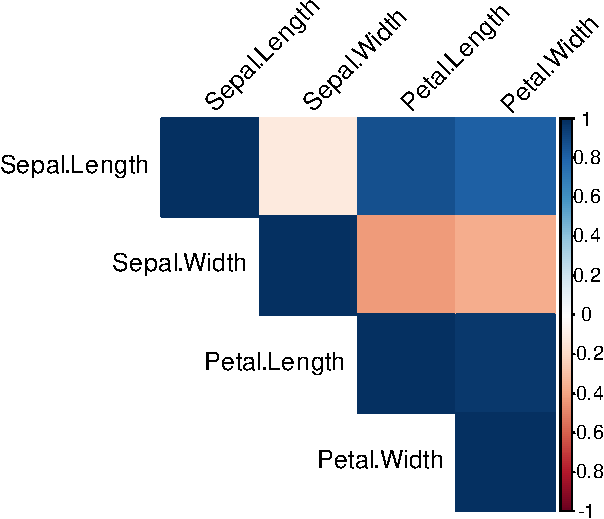
\includegraphics[keepaspectratio]{05-VA_gaussiane_files/figure-pdf/unnamed-chunk-25-1.pdf}}

}

\caption{Correlogramma del dataset Iris}

\end{figure}%

Il comando \texttt{plot()} applicato direttamente ai dati fornisce
invece un diagramma a dispersione (in inglese \emph{scatter plot}) di
tutte le possibili coppie.

\begin{Shaded}
\begin{Highlighting}[]
\FunctionTok{plot}\NormalTok{(iris[,}\DecValTok{1}\SpecialCharTok{:}\DecValTok{4}\NormalTok{], }\AttributeTok{col=}\NormalTok{miei\_colori[}\DecValTok{2}\NormalTok{], }\AttributeTok{pch=}\DecValTok{16}\NormalTok{)}
\end{Highlighting}
\end{Shaded}

\begin{center}
\pandocbounded{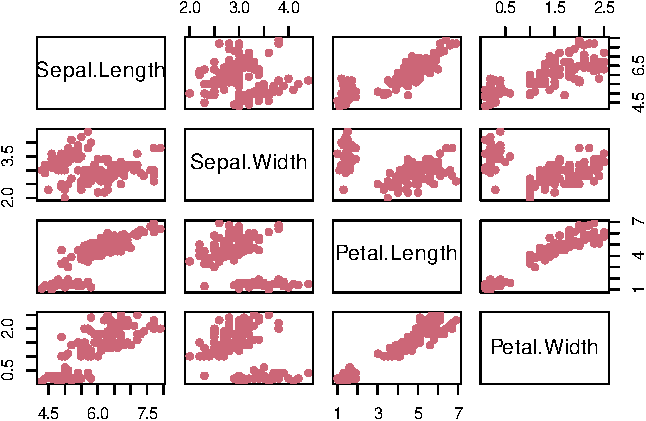
\includegraphics[keepaspectratio]{05-VA_gaussiane_files/figure-pdf/unnamed-chunk-26-1.pdf}}
\end{center}

Tralasciamo invece l'approccio bayesiano, più complesso.

\subsection{Esercizi}\label{esercizi-28}

Ripetere le osservazioni fatte sopra considerando separatamente ciascuna
specie (selezionare le prime 50 righe per la prima specie, le ulteriori
50 per la seconda e le ultime 50 per la terza).

Si scarichino dalla pagina del progetto \emph{Pageview stats},
https://pageviews.toolforge.org/, i dati relativi alle visualizzazioni
di \(4\) pagine di Wikipedia che si possano ritenere correlate (ad
esempio si parta da una pagina e si considerino poi il primo
collegamento da essa, oppure i primi due, e si ripeta). Si calcoli la
correlazione empirica e la si visualizzi graficamente.

\section{Analisi delle componenti principali (PCA)}\label{sec-pca}

Consideriamo in questa sezione un problema tipico del caso vettoriale,
che si può affrontare con tecniche simili a quelle introdotte sopra
(ossia usando medie e varianza campionarie e stima di massima
verosimiglianza). Il problema è di ``ridurre la dimensionalità'' (in
inglese \emph{dimension reduction}) di una variabile \(Y \in \R^d\) (o
similmente di un certo numero \(n\) osservazioni di tale variabile), con
\(d\) molto grande, ossia introdurre una variabile \(X \in \R^k\), con
\(k\) molto più piccolo di \(d\) in modo da ``riassumere''
l'informazione di \(Y\) in modo efficace. Questo può essere utile per
rappresentare graficamente \(Y\) (ad esempio se \(k=2\)) ma anche per
velocizzare l'esecuzione di algoritmi che in dimensione alta possono
risultare particolarmente lenti.

Per fare un'esempio concreto, la foto di un volto di una persona
incontrata per caso può essere presentata come una variabile \(Y\) a
valori in uno spazio molto grande (una dimensione per ogni pixel
nell'immagine). Tuttavia quando noi osserviamo un volto ne facciamo
automaticamente un ``riassunto'' tramite caratteristiche quali il colore
degli occhi, della pelle, dei capelli ecc. La variabile \(X\) contiene
un ``riassunto'' efficace di \(Y\) (per la nostra memoria, però, mentre
per una stampante certamente è più utile direttamente la \(Y\)).

Il problema è presente in tantissimi ambiti scientifici e le tecniche
per affrontarlo sono molteplici. Una delle tecniche più semplici, ma
comunque efficace, è l'\textbf{analisi delle componenti principali} (in
inglese \emph{principal component analysis}, abbreviato PCA). Dal punto
di vista astratto la PCA si può spiegare in modo semplice ricordando il
procedimento di \emph{standardizzazione} di un vettore aleatorio. Data
\(Y \in \R^d\), la matrice delle covarianze \(\Sigma_Y\) può essere
diagonalizzata tramite il teorema spettrale, ossia esiste
\(U_Y \in \R^{d\times d}\) ortogonale (\(U^T_Y = U^{-1}_Y\)) tale che
\[ U_Y \Sigma_Y U^T_Y = D_Y\] è diagonale (e contiene gli autovalori di
\(\Sigma_Y\)). Dal punto di vista delle variabili, questo significa che
tramite un cambio di coordinate, ossia definendo \(Y' = U_Y Y\), la
matrice delle covarianze di \(Y'\) è diagonale, e quindi le componenti
non sono correlate. A questo punto, volendo ``riassumere'' \(Y\), si
definisce \(X \in \R^k\) come la variabile congiunta delle \(k\)
coordinate di \(Y'\) che hanno varianza maggiore. Si riassume quindi
\(Y\) catturandone il sottospazio di dimensione \(k\) che presenta
maggiore ``variabilità'' dal punto di vista della covarianza. La
variabile \(X\) si ottiene proiettando \(Y\) su tale sottospazio, ossia
algebricamente mediante una matrice di proiezione ortogonale
\(\Pi_Y \in \R^{k \times d}\), e vale quindi \[ X = \Pi_Y Y.\]

L'idea teorica descritta sopra solleva almeno due problemi, uno pratico
e uno teorico: 1. spesso si dispone solamente di un certo numero \(n\)
di osservazioni \((y_1, \ldots, y_n)\) associate a variabili aleatorie
\((Y_1, \ldots, Y_n)\), tutte indipendenti tra loro e con la stessa
legge di \(Y\). Come stimare \(\Pi_Y\)? 2. la PCA è una procedura
\emph{ad-hoc} per questo problema oppure si può giustificare mediante le
regole del calcolo della probabilità?

Una soluzione per il primo problema è immediata: invece di considerare
la matrice delle covarianze teorica \(\Sigma_Y\) (che non è nota),
partendo dalle osservazioni \(y = (y_1, \ldots, y_n)\), si procede allo
stesso modo partendo però dalla matrice delle covarianze campionarie,
\[\Sigma_{y} = \frac 1 n \sum_{i=1}(y_i-\bar{y})(y_i-\bar{y})^T.\]
Ricordiamo infatti che è una matrice simmetrica e semi-definita
positiva. Il teorema spettrale applicato \(\Sigma_y\) determina allora
una matrice ortogonale \(U_y \in \R^{d\times d}\) e una matrice
diagonale \(D_y \in \R^{d\times d}\) (contenente gli autovalori di
\(\Sigma_y\)) tali che \[ U_y \Sigma_y U_y^T = D_y.\] A questo punto, si
definisce \(\Pi_y \in \R^{k \times d}\) come la matrice di proiezione
nel sottospazio associato alle direzioni dei \(k\) vettori di \(U_y\)
per cui le componenti nella diagonale (le varianze) sono il più grande
possibile. Il ``riassunto'' in questo caso non è una variabile \(X\) ma
il vettore delle osservazioni proiettate \(x_i = \Pi_y y_i\) (anche se
tipicamente ciò che interessa sono il sottospazio su cui si proietta e
gli autovalori associati).

Applichiamo la PCA in R usando la funzione specifica \texttt{prcomp()}
(in alternativa, la decomposizione spettrale di una matrice si può
ottenere in generale tramite il comando \texttt{eigen()}). Vediamo ad
esempio sul dataset Iris (applicandolo solo ai dati numerici, escludendo
la colonna della specie) :

\begin{Shaded}
\begin{Highlighting}[]
\NormalTok{iris\_PCA }\OtherTok{=} \FunctionTok{prcomp}\NormalTok{(iris[,}\DecValTok{1}\SpecialCharTok{:}\DecValTok{4}\NormalTok{])}
\end{Highlighting}
\end{Shaded}

L'oggetto risultate contiene diverse informazioni sulla PCA, come ad
esempio la base di vettori \(U\) (che è una matrice \(4\times 4\) in
questo caso),

\begin{Shaded}
\begin{Highlighting}[]
\NormalTok{iris\_PCA}\SpecialCharTok{$}\NormalTok{rotation}
\end{Highlighting}
\end{Shaded}

\begin{verbatim}
                     PC1         PC2         PC3        PC4
Sepal.Length  0.36138659 -0.65658877  0.58202985  0.3154872
Sepal.Width  -0.08452251 -0.73016143 -0.59791083 -0.3197231
Petal.Length  0.85667061  0.17337266 -0.07623608 -0.4798390
Petal.Width   0.35828920  0.07548102 -0.54583143  0.7536574
\end{verbatim}

e le deviazioni standard delle varie componenti (ossia la radice
quadrata dei vari autovalori della matrice delle covarianze empirica
\(\Sigma_y\), o della sua diagonalizzata \(D_y\)).

\begin{Shaded}
\begin{Highlighting}[]
\NormalTok{iris\_PCA}\SpecialCharTok{$}\NormalTok{sdev}
\end{Highlighting}
\end{Shaded}

\begin{verbatim}
[1] 2.0562689 0.4926162 0.2796596 0.1543862
\end{verbatim}

Inoltre vi sono già calcolate tutte le osservazioni trasformate tramite
la matrice \(U\), ossia una matrice che contiene i vettori \(Uy_i\)
(come righe). Di questa possiamo ad esempio plottare la prima colonna
(corrispondente alla direzione con varianza massima), o le prime due. La
PCA ha l'effetto in questo caso di ben separare le tre specie, o quanto
meno la prima dalle altre due, come evidenziamo con la diversa
colorazione.

\begin{Shaded}
\begin{Highlighting}[]
\FunctionTok{plot}\NormalTok{(iris\_PCA}\SpecialCharTok{$}\NormalTok{x[,}\DecValTok{1}\NormalTok{], }\AttributeTok{col=}\NormalTok{ miei\_colori[}\FunctionTok{as.numeric}\NormalTok{(iris}\SpecialCharTok{$}\NormalTok{Species)], }\AttributeTok{pch=}\DecValTok{16}\NormalTok{, }\AttributeTok{xlab =} \StringTok{"esemplare"}\NormalTok{, }\AttributeTok{ylab=}\StringTok{"valore"}\NormalTok{)}
\end{Highlighting}
\end{Shaded}

\begin{center}
\pandocbounded{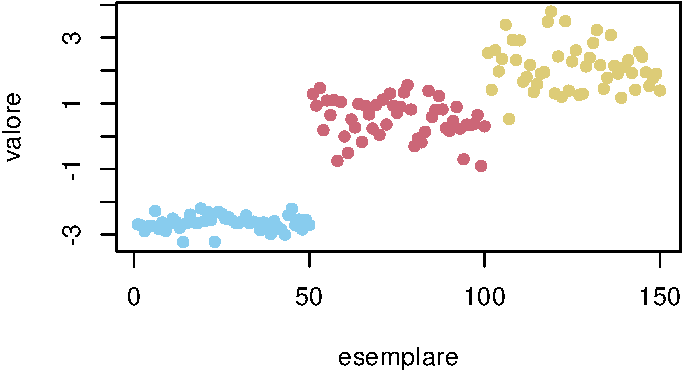
\includegraphics[keepaspectratio]{05-VA_gaussiane_files/figure-pdf/unnamed-chunk-30-1.pdf}}
\end{center}

\begin{Shaded}
\begin{Highlighting}[]
\FunctionTok{plot}\NormalTok{(iris\_PCA}\SpecialCharTok{$}\NormalTok{x[,}\DecValTok{1}\SpecialCharTok{:}\DecValTok{2}\NormalTok{], }\AttributeTok{col =}\NormalTok{ miei\_colori[}\FunctionTok{as.numeric}\NormalTok{(iris}\SpecialCharTok{$}\NormalTok{Species)], }\AttributeTok{pch=}\DecValTok{16}\NormalTok{)}
\end{Highlighting}
\end{Shaded}

\begin{center}
\pandocbounded{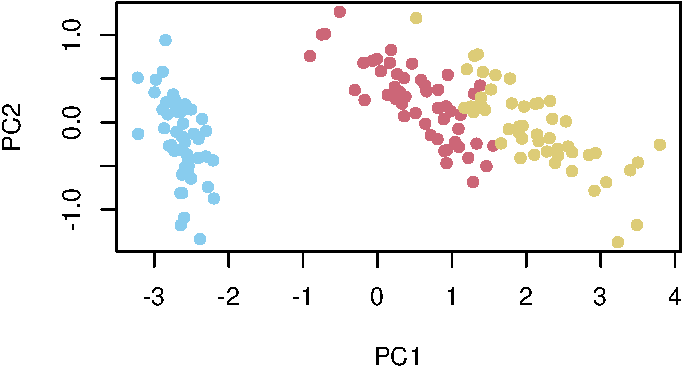
\includegraphics[keepaspectratio]{05-VA_gaussiane_files/figure-pdf/unnamed-chunk-31-1.pdf}}
\end{center}

Veniamo alla seconda domanda, e mostriamo che è possibile giustificare
il metodo di PCA in termini di una stima di massima verosimiglianza per
un opportuno modello gaussiano. L'idea è che con la PCA stiamo
recuperando un ``segnale'' (la \(X\)) osservandone una versione
``rumorosa'' e disposta su un sottospazio non noto.

Per introdurre un modello probabilistico, supponiamo fissata (e nota) la
dimensione \(k\) introduciamo una variabile standardizzata
\(Z \in \R^k\) e imponiamo che valga \[Y = AZ+W,\] dove
\(A \in \R^{d \times k}\) è una matrice non nota (rispetto
all'informazione priori). Il ``segnale'' da ricostruire è quindi \(AZ\)
(quello che nella PCA abbiamo chiamato \(X\)) e \(W\) è una variabile
che rappresenta il ``rumore'' aggiunto. Supponiamo che \(Z\), \(W\)
siano indipendenti con densità gaussiane centrate e, oltre a
\(\Sigma_Z = Id\), supponiamo che \(\Sigma_W = \sigma_0^2 Id\), per una
costante opportuna (nota a priori e sufficientemente piccola).
Supponendo nota la matrice \(A\), allora la densità di \(Y\), è
anch'essa una gaussiana centrata, con covarianza
\(\Sigma_Y =  AA^T + \sigma_0^2 Id\), chè è una funzione di \(A\).
Pertanto la verosimiglianza di \(A\) associata ad \(Y\) si scrive
\[L(A; y)  = p(Y=y | A) \propto \exp\bra{ - \frac 1 2 \bra{ y^T \sigma_Y^{-1} y + \log(\det(\Sigma_Y))  }}.\]
Ovviamente, se invece di una singola osservazione \(Y=y\), supponiamo di
avere \(n\) osservazioni indipendenti \(Y_i= y_i\), tutte gaussiane con
gli stessi parametri -- in particolare con la stessa matrice \(A\), la
verosimiglianza si ottiene come prodotto della funzione sopra (cambiando
i valori osservati)
\[ L(A; y_1, \ldots, y_n)  \propto \exp\bra{ - \frac n {2} \bra{ \frac 1 n\sum_{i=1}^n y_i^T \Sigma_Y^{-1} y_i + \log(\det(\Sigma_Y))  }}.\]
Per stimare \(A\) si tratta quindi di determinare
\(A \in \R^{d \times k}\) tale che la quantità sopra sia massima, ossia
(passando al solito all'opposto del logaritmo e minimizzando)
\[ A \mapsto \frac 1 n\sum_{i=1}^n y_i ^T \Sigma_Y^{-1} y_i + \log(\det(\Sigma_Y)\]
sia minima (ricordiamo che \(\Sigma_Y\) dipende da \(A\)). Riconosciamo
quindi una variante del problema della stima dei parametri di una
densità gaussiana vettoriale a partire da osservazioni indipendenti,
dove stavolta la dipendenza dei parametri (ossia \(A\)) è più complessa.
Tuttavia, con qualche passaggio di algebra lineare e calcolo in più
variabili si può dedurre che la stima di massima verosimiglianza per
\(A\) è data da
\[ A_{{\mle}} =  U_{y|k} (D_{y|k} - \sigma^2_0Id)^{1/2},\] dove
\(U_{y|k} \in \R^{d \times k}\) indica la matrice corrispondente ai
\(k\) autovettori della covarianza campionaria
\(\Sigma_y = \sum_{i=1}^n y_i y_i^T\) con autovalori più grandi, e
\(D_{y|k} \in \R^{k\times k}\) indica la matrice diagonale contenente
tali autovalori nell'ordine corrispondente. Tutto questo purché
\(\sigma_0^2\) sia sufficientemente piccolo, affinché la diagonale di
\(D_{y|k} - \sigma^2_0 Id\) sia positiva, altrimenti la radice quadrata
(intesa solamente sulla diagonale) non avrebbe senso. Nel limite
\(\sigma_0 \to 0\) si ottiene che \(A_{{\mle}}= U_{y|k} D_{y|k}^{1/2}\)
e la variabile \(A_{{\mle}}X\) si identifica con \(\Pi_y Y\)
(identificando \(\R^k\) con il sottospazio generato dai \(k\) vettori
delle colonne di \(U_{y|k}\)).

\subsection{Esercizi}\label{esercizi-29}

Si consideri il dataset `mtcars' contenente dati relativi ad alcuni
modelli di auto (ormai d'epoca). Si usi opportuni comandi R per
calcolare e visualizzare la matrice delle correlazioni campionarie e
successivamente si applichi la PCA e si plotti un diagramma a nuvola di
punti relativo alle prime due componenti principali.

Si consideri un dataset ricavato dalle visualizzazioni di pagine di
Wikipedia (https://pageviews.toolforge.org/) costruito come
nell'esercizio della sezione precedente. Si applichi la PCA e si plotti
un diagramma a nuvola di punti relativo alle prime due componenti
principali.

\section{Regressione (metodo dei minimi
quadrati)}\label{sec-regressione}

In questa sezione introduciamo il problema generale della regressione,
concentrandoci in particolare sul caso lineare con errore quadratico,
tradizionalmente detto anche \textbf{metodo dei minimi quadrati}
(\emph{ordinary least squares}, OLS, in inglese).

Il problema della regressione, in generale, si può descrivere nel
seguente modo: date due variabili aleatorie \(X \in E\), \(Y \in E'\)
determinare una funzione \(g: E \to  E'\) tale che \(Y\) sia ``molto
vicina'' a \(g(X)\), \[ Y \sim g(X),\] a partire dall'osservazione
congiunta di \((X,Y)\) (sottoforma di una o più copie, solitamente
indipendenti). La variabile \(X\) è detta \textbf{predittore} (in
inglese \emph{predictor}) o \textbf{variabile esplicativa}
(\emph{explanatory variable}), mentre la variabile \(Y\) è detta
\textbf{risposta} (\emph{response}) oppure \textbf{esito}
(\emph{outcome}). Evitiamo appositamente il linguaggio trazionale di
variabile ``indipendente'' (che sarebbe la \(X\)) e ``dipendente'' (la
\(Y\)) per evitare di confonderlo con il concetto probabilistico di
indipendenza.

In molte applicazioni, \(X\) è una variabile vettoriale, ossia
\(E=\R^d\) (se \(d >1\) si parla di regressione multipla), mentre a
seconda dell'obiettivo che ci si pone, \(Y\) potrebbe anche essere una
variabile discreta (noi ci concentreremo al caso in cui sia una varibile
continua, eventualmente anch'essa vettoriale).

La regressione si usa anche per problemi di classificazione, in cui ad
esempio bisogna ``etichettare'' i possibili valori di \(X\) per
determinare due (o più) classi disgiunte e quindi la variabile di
risposta \(g(X)\) è discreta a valori nell'insieme delle possibili
etichette.

Dal punto di vista del calcolo delle probabilità, essendo l'incognita
\(g\) non nota e di solito non completamente determinata
dall'osservazione di \((X,Y)\), si introduce una variabile aleatoria
\(G\) a valori nell'insieme delle possibili funzioni da \(E\) in \(E'\).
Il problema diventa quindi determinare la legge di \(G\) sulla base
dell'informazione a priori \(I\) e dei dati osservati, ossia \((X,Y)\).
La regressione generalizza quindi in senso probabilistico il concetto di
``curva interpolante'', o più in generale il problema di determinare una
funzione il cui grafico passi per determinati punti \((x,y)\). Questa
generalizzazione avviene almeno su due fronti: 1. da un lato \(G\) non è
una singola funzione ma una densità di probabilità sulle funzioni
(ovviamente poi si dovrà scegliere una stima, ad esempio tramite massima
verosimiglianza, ossia la funzione \(g\) tale che la probabilità di
osservare \(G=g\) sia massima) 2. dall'altro si introduce una ulteriore
flessibilità non richiedendo che la curva interpoli esattamente i punti
osservati, ma introducendo un certo ``residuo'' (o errore), definito
spesso come la differenza tra \(Y\) e \(G(X)\) ossia \(Y-G(X)\).

Pertanto, almeno in teoria, tutto il problema si riduce, come in altre
situazioni, a specificare una densità a priori per la variabile
aleatoria \(G\) e usare la formula di Bayes per stimarla dopo le
osservazioni \((X,Y)\), o in alternativa usare la stima di massima
verosimiglianza. Tuttavia, in pratica, l'insieme delle funzioni da \(E\)
in \(E'\) è troppo grande per essere trattato agevolmente (sia
numericamente che analiticamente), e perciò si specifica un
\emph{modello}, ossia una opportuna famiglia parametrizzata di funzioni
da \(E\) in \(E'\). Questo fatto può anche essere visto come un modo di
introdurre una certa informazione a priori sulla struttura della
funzione, non nota, ma neppure totalmente arbitraria.

Tecnicamente, per specificare un modello si suppone che la variabile
aleatoria \(G\) (a valori nelle funzioni da \(E\) in \(E'\)) sia una
variabile composta tramite un ``parametro'' \(U\) (che possiamo supporre
aleatorio, essendo non noto a priori), solitamente a valori in uno
spazio vettoriale \(\R^k\) con dimensione \(k\), piccola rispetto alla
dimensione dello spazio di tutte le possibili funzioni. Pertanto, per
ogni possibile valore \(U=u\) del parametro, è definita una funzione
\(g( \cdot ; u): E \to E'\) che ad ogni \(x \in E\) associa
\(g(x; u) \in E'\). Per chiarire le idee, vediamo degli esempi
fondamentali.

L'esempio piu semplice, su cui ci soffermeremo maggiormente, è il caso
in cui \(E' = \R^{d'}\) e la funzione \(G\) sia \emph{lineare} nel
parametro \(U\in \R^k\), cioè che l'associazione
\[ u \in \R^k \mapsto g( \cdot ; u) \] sia lineare, della forma
\[ g(x; u) = \sum_{i=1}^k g_i(x) u_i\] per opportune funzioni (note e
fissate a priori) \(g_i: E \to E' = \R^{d'}\). Notiamo che le singole
funzioni \(g_i\), \(x \mapsto g_i(x)\), possono essere anche \emph{non}
lineari, come ad esempio \(g(x) = x^2\), anche se in molti casi pure lo
sono. Il punto è che si può sempre considerare, al posto della variabile
esplicativa \(X\), la variabile congiunta \(X' = (g_i(X))_{i=1}^k\), in
modo che quindi si possa scrivere la dipendenza come se fosse lineare,
\[ g(x; u) = \sum_{i=1}^k x_i' u_i.\] Ad esempio, il modello
\[g(x; (u_1, u_2)) = u_1 x+ u_2 x^2\] è lineare (in \(u\)) ma non in
\(x\), tuttavia diventa lineare se lo si pensa in termini della nuova
variabile \(X' = (X, X^2)\).

Un altro punto che non viene spesso evidenziato è che anche un modello
``affine'' ossia \[ g(x; u) = u_0 + \sum_{i=1}^k x_i u_i \] è in realtà
lineare, perché lo è nella variabile \(u = (u_0, u_1, \ldots, u_k)\),
mentre alle \(g_i = x_i\) va aggiunta la \(g_0 = 1\) costante.

Un esempio di modello non lineare si ottiene componendo un modello
lineare tramite una funzione non lineare, come ad esempio la funzione
logistica (detta anche sigmoide per la forma del grafico)
\(\ell: \R \to (0,1)\), \[\ell(z) = \frac{1}{1+e^{-z}}.\]

\begin{Shaded}
\begin{Highlighting}[]
\NormalTok{deltaz}\OtherTok{=} \FloatTok{0.01}
\NormalTok{z }\OtherTok{=} \FunctionTok{seq}\NormalTok{(}\SpecialCharTok{{-}}\DecValTok{6}\NormalTok{,}\DecValTok{6}\NormalTok{, }\AttributeTok{by=}\NormalTok{deltaz)}
\NormalTok{l\_z }\OtherTok{=} \DecValTok{1}\SpecialCharTok{/}\NormalTok{(}\DecValTok{1}\SpecialCharTok{+}\FunctionTok{exp}\NormalTok{(}\SpecialCharTok{{-}}\NormalTok{z))}
\FunctionTok{plot}\NormalTok{(z, l\_z, }\AttributeTok{type=}\StringTok{\textquotesingle{}l\textquotesingle{}}\NormalTok{, }\AttributeTok{lwd =}\DecValTok{3}\NormalTok{, }\AttributeTok{col=}\NormalTok{miei\_colori[}\DecValTok{2}\NormalTok{], }\AttributeTok{xlab=}\StringTok{\textquotesingle{}z\textquotesingle{}}\NormalTok{, }\AttributeTok{ylab=}\StringTok{\textquotesingle{}l(z)\textquotesingle{}}\NormalTok{)}
\end{Highlighting}
\end{Shaded}

\begin{figure}[H]

{\centering \pandocbounded{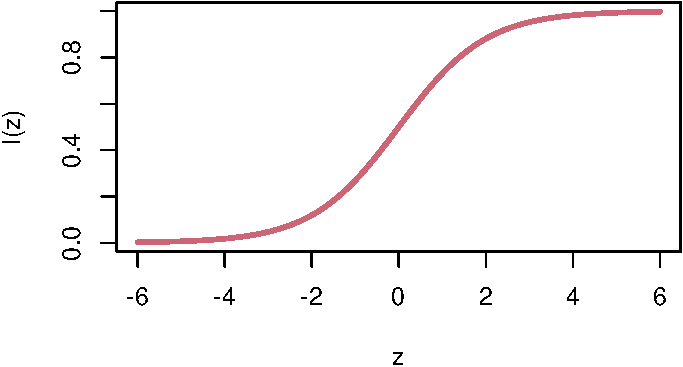
\includegraphics[keepaspectratio]{05-VA_gaussiane_files/figure-pdf/unnamed-chunk-32-1.pdf}}

}

\caption{grafico della funzione logistica \(\ell\)}

\end{figure}%

Si ottiene pertanto un modello della forma
\[ g(x; u) = \ell\bra{ \sum_{i=1}^k g_i(x) u_i} = \frac{1}{1+\exp\bra{-\sum_{i=1}^k g_i(x) u_i}}. \]
per delle opportune funzioni \(g_i(x)\). La regressione basata su tali
modelli è detta appunto \emph{logistica} e viene spesso usata per
problemi di classificazione binaria (ossia per partizionare i valori di
\(X\) in due classi, corrispondenti a \(\cur{Y\le 1/2}\) e \({Y>1/2}\).

Presentiamo ora il classico metodo dei minimi quadrati con la notazione
introdotta sopra: si suppone \(Y \in E' = \R^{d'}\) e \(U \in \R^k\),
per cui si può introdurre, come misura dell'errore nell'approssimazione
di \(Y\) mediante \(g(X;U)\) la differenza \(Y-g(X;U)\), detta anche
\textbf{residuo}. Il metodo consiste quindi, avendo osservato \(X=x\),
\(Y=y\), nel determinare un valore del parametro che minimizzi il
``residuo quadratico'', ossia
\[  u_{\ols} \in \operatorname{arg} \min_{u \in \R^k} |y - g(x; u)|^2,\]
Più in generale, di solito si dispone di \(n\) osservazioni indipendenti
di coppie di variabili \((X_i,Y_i) =(x_i,y_i)\) per cui si suppone che
il parametro \(U\) da stimare sia lo stesso, ossia
\(Y_i \sim g(X_i, U)\), allora il metodo consiste nel minimizzare la
somma dei residui quadratici:
\[ u_{\ols} \in  \operatorname{arg} \min_{u \in \R^k}\sum_{i=1}^n |y_i - g(x_i; u)|^2.\]
Il metodo indica anche, come stima della ``varianza'' del residuo tipico
\(Y-g(X; u_{\ols})\), la quantità detta anche \textbf{errore quadratico
medio} (in inglese \emph{mean squared error}, MSE)
\[ \frac 1 n \sum_{i=1}^n |y_i - g(x_i; u_{\ols})|^2,\] anche se, come
per la varianza campionaria, il denominatore \(n\) è solitamente
sosituito con il numero \(n-k\) di ``gradi di libertà'' per ottenerne
una stima ``non distorta'' (\emph{unbiased}) -- questo non cambia molto
fintanto che il numero dei parametri \(k\) è molto più piccolo del
numero delle osservazioni \(n\), cosa che avviene solitamente.

Consideriamo il caso di \(X\), \(Y\) a valori reali e un modello lineare
parametrizzato da \(u=(a,b) \in \R^2\), ossia \[ g(x; u) = ax +b\] Per
il metodo dei minimi quadrati, avendo \(n\) osservazioni indipenenti
(supponendole tutte con il medesimo parametro \((a,b)\) da stimare) si
deve quindi minimizzare la somma dei residui
\[ \sum_{i=1}^n (y_i - a x_i -b)^2,\] come funzione di \((a,b)\).
Imponendo che le derivate si annullino si trova un semplice sistema
(lineare) nelle incognite \(a\), \(b\), che risolto permette di
determinare
\[ a_{\ols} = \frac{  \sum_{i=1}^n(y_i - \bar{y})(x_i - \bar{x})}{ \sum_{i=1}^n (x_i- \bar{x})^2} = \frac{ \Sigma_{xy}}{\Sigma_{xx}}\]
avendo indicato con \(\Sigma\) le covarianze campionarie, e
\[ b_{\ols} = \bar{y} - \frac{ \Sigma_{xy}}{\Sigma_{xx}} \bar{x}.\] In
particolare, notiamo che il segno di \(a_{\ols}\) coincide con quello
della covarianza campionaria \(\Sigma_{xy}\) (essendo la varianza a
denominatore sempre positiva). Recuperiamo quindi il significato di
positiva (o negativa) correlazione in termini della ``concentrazione''
della densità della variabile congiunta \((X,Y)\) intorno ad una retta
con coefficiente angolare positivo (o negativo). Si può anche esprimere
in alternativa
\[ a_{\ols} = \rho_{xy} \frac{\sigma_y}{\sigma_x}, \quad b_{\ols} = \bar{y} - \rho_{xy} \frac{ \sigma_y}{\sigma_x} \bar{x}\]
usando il coefficiente di correlazione e le deviazioni standard
campionarie
\[ \sigma_x = \sqrt{ \Sigma_{xx}}, \quad \sigma_y = \sqrt{ \Sigma_{yy}}, \quad \rho_{xy} = \frac{\Sigma_{xy}}{\sigma_x \sigma_y}.\]

In R la regressione su un modello lineare è implementata tramite la
funzione \texttt{lm()}. Vediamo un esempio basandoci sulle osservazioni
del dataset Iris. Si vuole predire la lunghezza del sepalo (prima
colonna) a partire da quella del petalo (terza colonna). Il parametro di
intercetta \(b\) è aggiunto automaticamente, non serve specificarlo.

\begin{Shaded}
\begin{Highlighting}[]
\CommentTok{\# la funzione y = u\_0 + u\_1x\_1 + ... + u\_k x\_k è specificata introducendo una  formula del tipo y \textasciitilde{}  x1 + x2+ ... + xk, dove le xi sono le colonne del data frame.  Non serve specificare l\textquotesingle{}intercetta perché è introdotta automaticamente. (Per formule complicate vi sono anche altri modi di inserirle)}

\NormalTok{x }\OtherTok{=}\NormalTok{ iris}\SpecialCharTok{$}\NormalTok{Petal.Length}
\NormalTok{y }\OtherTok{=}\NormalTok{ iris}\SpecialCharTok{$}\NormalTok{Sepal.Length}

\NormalTok{iris\_reg\_lin }\OtherTok{=} \FunctionTok{lm}\NormalTok{( y }\SpecialCharTok{\textasciitilde{}}\NormalTok{ x )}



\CommentTok{\# L\textquotesingle{}output della funzione è una lista contenente diverse informazioni utili, tra cui i coefficienti}

\NormalTok{iris\_reg\_lin}\SpecialCharTok{$}\NormalTok{coefficients}
\end{Highlighting}
\end{Shaded}

\begin{verbatim}
(Intercept)           x 
  4.3066034   0.4089223 
\end{verbatim}

\begin{Shaded}
\begin{Highlighting}[]
\CommentTok{\# i residui y\_i {-} g(x\_i, u), che possiamo plottare con un istogramma}

\FunctionTok{hist}\NormalTok{(iris\_reg\_lin}\SpecialCharTok{$}\NormalTok{residuals, }\AttributeTok{col=}\NormalTok{miei\_colori[}\DecValTok{1}\NormalTok{], }\AttributeTok{probability =} \ConstantTok{TRUE}\NormalTok{, }\AttributeTok{xlab=}\StringTok{"residui"}\NormalTok{, }\AttributeTok{ylab=}\StringTok{"densità"}\NormalTok{)}
\end{Highlighting}
\end{Shaded}

\begin{center}
\pandocbounded{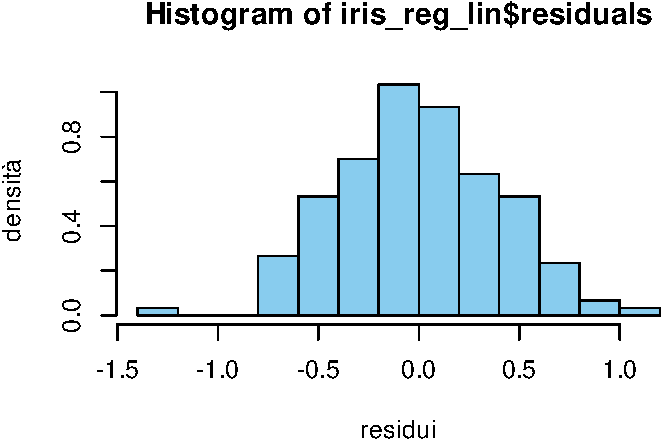
\includegraphics[keepaspectratio]{05-VA_gaussiane_files/figure-pdf/unnamed-chunk-33-1.pdf}}
\end{center}

\begin{Shaded}
\begin{Highlighting}[]
\CommentTok{\# e i valori "previsti" dal modello con i parametri ottenuti, che possiamo plottare accanto a quelli osservati}

\FunctionTok{plot}\NormalTok{( x,y, }\AttributeTok{type=}\StringTok{\textquotesingle{}p\textquotesingle{}}\NormalTok{, }\AttributeTok{pch=}\DecValTok{16}\NormalTok{, }\AttributeTok{col=}\NormalTok{miei\_colori[}\DecValTok{1}\NormalTok{], }\AttributeTok{xlab =} \StringTok{\textquotesingle{}lunghezza del petalo\textquotesingle{}}\NormalTok{, }\AttributeTok{ylab=}\StringTok{\textquotesingle{}lunghezza del sepalo\textquotesingle{}}\NormalTok{)}

\FunctionTok{points}\NormalTok{( x, iris\_reg\_lin}\SpecialCharTok{$}\NormalTok{fitted.values, }\AttributeTok{pch=}\DecValTok{16}\NormalTok{, }\AttributeTok{col=}\NormalTok{miei\_colori[}\DecValTok{2}\NormalTok{])}

\FunctionTok{legend}\NormalTok{(}\StringTok{\textquotesingle{}bottomright\textquotesingle{}}\NormalTok{,  }\AttributeTok{fill=}\NormalTok{miei\_colori[}\DecValTok{1}\SpecialCharTok{:}\DecValTok{2}\NormalTok{], }\AttributeTok{legend=}\FunctionTok{c}\NormalTok{(}\StringTok{"osservati"}\NormalTok{, }\StringTok{"previsti"}\NormalTok{))}

\CommentTok{\# possiamo anche aggiungere una linea per meglio rappresentare la retta interpolante del modello con il comando abline()}

\FunctionTok{abline}\NormalTok{(iris\_reg\_lin}\SpecialCharTok{$}\NormalTok{coefficients, }\AttributeTok{col=}\NormalTok{miei\_colori[}\DecValTok{2}\NormalTok{], }\AttributeTok{lwd=}\DecValTok{2}\NormalTok{)}
\end{Highlighting}
\end{Shaded}

\begin{center}
\pandocbounded{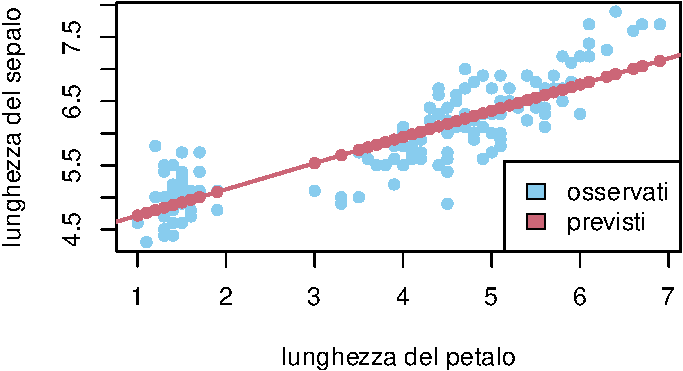
\includegraphics[keepaspectratio]{05-VA_gaussiane_files/figure-pdf/unnamed-chunk-33-2.pdf}}
\end{center}

\begin{Shaded}
\begin{Highlighting}[]
\CommentTok{\# introduciamo un data frame con le nuove osservazioni di lunghezze di petali}

\NormalTok{x\_osservati }\OtherTok{=} \FunctionTok{data.frame}\NormalTok{( }\AttributeTok{x=} \FunctionTok{c}\NormalTok{(}\DecValTok{2}\NormalTok{, }\FloatTok{2.2}\NormalTok{, }\FloatTok{2.5}\NormalTok{, }\DecValTok{3}\NormalTok{))}

\NormalTok{y\_previsti }\OtherTok{=} \FunctionTok{predict}\NormalTok{(iris\_reg\_lin, x\_osservati)}

\CommentTok{\# rappresentiamo le previsioni in un nuovo plot}


\FunctionTok{plot}\NormalTok{( x,y, }\AttributeTok{type=}\StringTok{\textquotesingle{}p\textquotesingle{}}\NormalTok{, }\AttributeTok{pch=}\DecValTok{16}\NormalTok{, }\AttributeTok{col=}\NormalTok{miei\_colori[}\DecValTok{1}\NormalTok{], }\AttributeTok{xlab =} \StringTok{\textquotesingle{}lunghezza del petalo\textquotesingle{}}\NormalTok{, }\AttributeTok{ylab=}\StringTok{\textquotesingle{}lunghezza del sepalo\textquotesingle{}}\NormalTok{)}

\FunctionTok{points}\NormalTok{( x\_osservati}\SpecialCharTok{$}\NormalTok{x, y\_previsti, }\AttributeTok{pch=}\DecValTok{16}\NormalTok{, }\AttributeTok{col=}\NormalTok{miei\_colori[}\DecValTok{2}\NormalTok{])}

\FunctionTok{legend}\NormalTok{(}\StringTok{\textquotesingle{}bottomright\textquotesingle{}}\NormalTok{,  }\AttributeTok{fill=}\NormalTok{miei\_colori[}\DecValTok{1}\SpecialCharTok{:}\DecValTok{2}\NormalTok{], }\AttributeTok{legend=}\FunctionTok{c}\NormalTok{(}\StringTok{"osservazioni"}\NormalTok{, }\StringTok{"previsioni"}\NormalTok{))}

\CommentTok{\# notiamo che sono tutti sulla retta di regressione }

\FunctionTok{abline}\NormalTok{(iris\_reg\_lin}\SpecialCharTok{$}\NormalTok{coefficients, }\AttributeTok{col=}\NormalTok{miei\_colori[}\DecValTok{2}\NormalTok{], }\AttributeTok{lwd=}\DecValTok{2}\NormalTok{)}
\end{Highlighting}
\end{Shaded}

\begin{center}
\pandocbounded{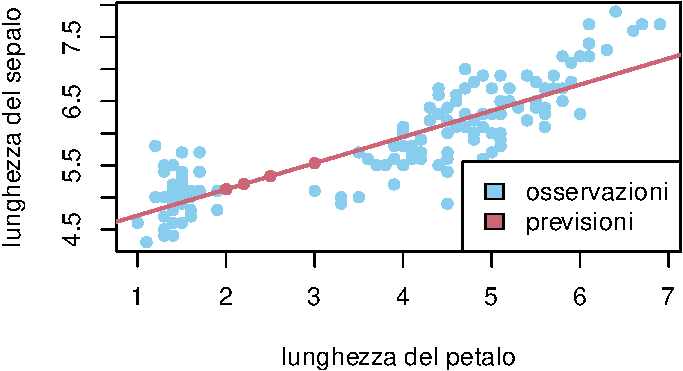
\includegraphics[keepaspectratio]{05-VA_gaussiane_files/figure-pdf/unnamed-chunk-34-1.pdf}}
\end{center}

Consideriamo ora un modello lineare più generale (multipla), in cui
\(X \in\R^d\), \(U \in \R^{k}\), \(Y \in \R\) e
\[ g(x; u) =  \sum_{j=1}^k x_j u_j = x \cdot u,\] indicando con
\(\cdot\) il prodotto scalare in \(\R^k\) per alleggerire la notazione.
Avendo osservato \(X_i= x_i\), \(Y_i =y_i\) per \(i= 1, \ldots, n\), il
metodo dei minimi quadrati consiste nel minimizzare la funzione
\[ u \mapsto \sum_{i=1}^n (y_i -  x_i \cdot u)^2,\] che è una funzione
\emph{quadratica} nelle variabili \(u = (u_j)_{j=1}^k\). Pertanto,
imponendo che le derivate parziali si annullino si ottiene un sistema
lineare (di \(k\) equazioni in \(k\) incognite) che ammette come
soluzione esplicita il vettore \[ u_{\ols} = (x^T x)^{-1} x^Ty,\] dove
\(x \in \R^{n \times d}\) è intesa come matrice le cui righe sono le
osservazioni \(x_i \in \R^d\) e si suppone che la matrice
\(x^Tx\in \R^{d \times d}\) sia invertibile. (tale matrice è gioca un
ruolo simile alla matrice delle covarianze campionarie). La previsione è
quindi data dalla funzione
\[ z \mapsto g(z, u_{\ols}) = z \cdot (x^T x)^{-1} x^Ty.\]

Il comando \texttt{lm()} permette di effettuare regressione lineare
multipla in dimensione arbitraria. Ad esempio, possiamo considerare come
predittori della lunghezza del sepalo nel dataset Iris tutte le
variabili (eccetto la specie).

\begin{Shaded}
\begin{Highlighting}[]
\NormalTok{iris\_reg\_gen }\OtherTok{=} \FunctionTok{lm}\NormalTok{( Sepal.Length  }\SpecialCharTok{\textasciitilde{}}\NormalTok{ Sepal.Width }\SpecialCharTok{+}\NormalTok{Petal.Length }\SpecialCharTok{+}\NormalTok{ Petal.Width, }\AttributeTok{data =}\NormalTok{ iris)}

\CommentTok{\# Possiamo avere un "riassunto" della regressione con il comando summary()}

\FunctionTok{summary}\NormalTok{(iris\_reg\_gen)}
\end{Highlighting}
\end{Shaded}

\begin{verbatim}

Call:
lm(formula = Sepal.Length ~ Sepal.Width + Petal.Length + Petal.Width, 
    data = iris)

Residuals:
     Min       1Q   Median       3Q      Max 
-0.82816 -0.21989  0.01875  0.19709  0.84570 

Coefficients:
             Estimate Std. Error t value Pr(>|t|)    
(Intercept)   1.85600    0.25078   7.401 9.85e-12 ***
Sepal.Width   0.65084    0.06665   9.765  < 2e-16 ***
Petal.Length  0.70913    0.05672  12.502  < 2e-16 ***
Petal.Width  -0.55648    0.12755  -4.363 2.41e-05 ***
---
Signif. codes:  
0 '***' 0.001 '**' 0.01 '*' 0.05 '.' 0.1 ' ' 1

Residual standard error: 0.3145 on 146 degrees of freedom
Multiple R-squared:  0.8586,    Adjusted R-squared:  0.8557 
F-statistic: 295.5 on 3 and 146 DF,  p-value: < 2.2e-16
\end{verbatim}

Con la funzione \texttt{summary()} usata nell'esempio sopra si leggono
anche altre informazioni rilevanti, come la stima della deviazione
standard dei residui (detta anche \textbf{errore standard} dei residui,
in inglese \emph{residual standard error}) definita come la radice
quadrata della versione ``non distorta'' dell'errore quadratico medio,
\[ s = \sqrt{ \frac{1}{n-k} \sum_{i=1}^n|y_i - x_i \cdot u_{\ols}|^2}.\]
Inoltre, ciascun parametro stimato, ossia ogni componente del vettore
\(u_{OLS}\) è accompagnato da una stima della deviazione standard
(visibile nella seconda colonna \emph{Std. Error}, accanto a quella
contenente la stima \emph{Estimate}), definito per la componente
\(j \in \cur{1, \ldots, k}\) come la quantità
\[  s_j = s \sqrt{ (x^Tx)^{-1}_{jj}}.\]

\begin{remark}[varianza spiegata]
Una quantità spesso utilizzata per valutare l'efficacia della
regressione è il \textbf{coefficiente di determinazione} (in inglese
\emph{coefficient of determination}) definito come
\[ R^2 =  1- \frac{ \sum_{i=1}^n |y_i -x_i \cdot u_{\ols}|^2}{ \sum_{i=1}^n |y_i - \bar{y}|^2},\]
dove riconosciamo (a meno di moltiplicare per \(1/n\) numeratore e
denominatore) l'errore quadratico medio e la varianza campionaria. Esso
è una quantità minore (o uguale) ad \(1\), e misura l'aderenza del
modello lineare ai dati osservati, confrontandolo con il caso di un
modello ``costante'' (per cui si otterrebbe come miglior funzione la
media campionaria). Più \(R^2\) risulta vicino ad \(1\), migliore è
l'aderenza ai dati osservati. Se nel modello lineare è inclusa la
funzione costante, come è automatico nella funzione \texttt{lm()},
allora si può mostrare che \(R^2\) è anche non negativo, quindi sempre
compreso tra \(0\) ed \(1\). In questo senso si intepreta come la
``percentuale'' di varianza (dei dati) spiegata dal modello lineare
preso in considerazione.

Idealmente si vorrebbe \(R^2\) molto grande, ma bisogna prestare
attenzione al fatto che una aderenza eccessiva ai dati, ossia \(R^2\)
troppo vicino ad \(1\) potrebbe essere un segnale di \textbf{overfit},
in cui i parametri introdotti sono troppi (ossia la dimensione \(k\) è
troppo grande in confronto al numero di osservazioni \(n\)) e la
funzione stimata ``insegue'' le osservazioni senza veramente
``imparare'' nulla da esse, ossia fornendo previsioni poco efficaci se
testato nuove osservazioni della variabile dipendente. Per superare
parzialmente questo problema, si usa una versione ``aggiustata'' del
coefficiente (in inglese \emph{adjusted} \(R^2\)), anch'essa indicata
nel comando \texttt{summary()}
\end{remark}

Per meglio comprendere il metodo dei minimi quadrati, ne vediamo ora una
intepretazione in termini di stima di massima verosimiglianza. Questo,
oltre a dare una giustificazione teorica basata sul calcolo delle
probabilità permette anche di comprendere meglio alcune ipotesi che ne
permettono una applicazione corretta.

Con la notazione sopra, introduciamo un modello probabilistico tale che,
rispetto ad una informazione a priori (prima delle osservazioni),
\(X \in E\), \(Y \in E = \R^{d'}\), \(U \in \R^k\) siano variabili
aleatorie per cui \[ Y = g(X;U) + W,\] dove \(W\) è una variabile
(indicante il residuo) con densità gaussiana vettoriale
\(\mathcal{N}(0, v Id)\) (dove \(v>0\) è un parametro), e che le tre
variabili \(X\), \(U\) e \(W\) siano tra loro indipendenti. Solamente
con queste ipotesi, qualsiasi sia la densità a priori di \(X\), si
ottiene come funzione di verosimiglianza
\[ \begin{split} L(u ; x, y) & = p(X=x, Y=y |  U = u) \\
&= p(Y=y| U=u, X=x) p(X=x| U=u)\\
& = p( Y-g(x;u) = y-g(x;u) | U=u, X=x) p(X=x) \\
& = p( W = y-g(x,u) | U=u, X=x) p(X=x)\\
& =  \exp\bra{ -\frac 1 {2v} |y-g(x,u)|^2 }\frac{1}{\sqrt{ 2 \pi v}} p(X=x).
\end{split}\] Avendo osservato \(X=x\), \(Y=y\), la stima di massima
verosimiglianza per \(U\) consiste quindi nel determinare il minimo
della quantità \[  u \mapsto |y-g(x,u)|^2, \] ossia il minimo residuo
quadratico. Similmente, se invece si dispone di \(n\) variabili
\((X_i, W_i)\) tutte indipendenti tra loro (e indipendenti da una
variabile \(U\)) tali che, per ogni \(i=1, \ldots, n\) valga
\[ Y_i = g(X_i; U) + W_i,\] allora la funzione di verosimiglianza per
\(U\) associata alle osservazioni \(X_i=  x_i\), \(Y_i = y_i\) diventa,
con calcoli analoghi e scrivendo per brevità \(x = (x_i)_{i=1}^n\),
\(y= (y_i)_{i=1}^n\),
\[ \begin{split} L(u ; x, y) & = p(X=x, Y=y |  U = u) \\
& =  \exp\bra{ -\frac 1 {2 v} \sum_{i=1}^n |y_i-g(x_i,u)|^2 }\frac{1}{\sqrt{ (2 \pi v)^n}} \prod_{i=1}^n p(X_i=x_i).\end{split}\]
E quindi, qualsiasi sia la densità di \(X_i\) (anche non necessariamente
la stessa per tutte le osservazioni) si trova che la stima di massima
verosimiglianza per \(U\) è tale che la funzione
\[ u \mapsto \sum_{i=1}^n |y_i-g(x_i,u)|^2,\] sia minima, quindi la
stima \(u_{\ols}\) indicata dal metodo dei minimi quadrati.

Inoltre, poiché nelle espressioni sopra abbiamo mantenuta esplicita la
dipendenza dal parametro \(v\) (la varianza del residuo \(W\)), pensando
la verosimiglianza anche come funzione di tale parametro, con gli stessi
calcoli per la stima del parametro varianza di una gaussiana a partire
da osservazioni indipendenti (è in effetti questa la situazione),
otteniamo che la stima di massima verosimiglianza per la coppia
\((u, v)\) è
\[ u_{\mle } = u _{\ols} \in  \arg \min_{u \in \R^k} \sum_{i=1}^n |y_i-g(x_i;u)|^2\]
e l'errore quadratico medio (nella versione ``distorta'')
\[ v_{\mle} = MSE = \frac 1 n \sum_{i=1}^n |y_i-g(x_i;u)|^2.\]

\begin{remark}
La giustificazione sopra si basa essenzialmente sull'ipotesi (a priori)
che i residui siano variabili gaussiane indipendenti con gli stessi
parametri (e media nulla). Questa ipotesi non si può giustificare prima
di applicare il metodo, tuttavia è possibile, dopo l'applicazione,
considerarne la validità, almeno qualitativamente oppure tramite test
(si veda la Sezione Sezione~\ref{sec-test}).
\end{remark}

Questa derivazione del metodo dei minimi quadrati come stima di massima
verosimiglianza suggerisce anche un approccio bayesiano, in cui una
densità a priori su \(U\) possa racchiudere dell'informazione già nota
sul problema. Ad esempio, supponiamo che sia noto a priori che \(U\) non
si discosta troppo da un parametro noto \(u_0\), ad esempio con una
variabilità dell'ordine di \(\sigma_u>0\) (lungo ciascuna componente) e
che le componenti di \(U\) siano indipendenti tra loro. Questo si
traduce nell'assumere che la densità a priori per \(U\) sia vettoriale
gaussiana \(\mathcal{N}(u_0, \sigma_u^2 Id)\), e quindi la formula di
Bayes darebbe, dopo \(n\) osservazioni \(X_i =x_i\), \(Y_i= y_i\) (con
le ipotesi sopra di indipendenza)
\[ \begin{split}&  p(U = u | X_i=x_i, Y_i= y_i, \,  \forall i=1, \ldots, n) \\
& \propto \exp\bra{ -\frac 1 {2\sigma_u^2} |u-u_0|^2} L(u; x, y)\\
& \propto \exp\bra{ -\frac 1 {2} \bra{ \frac 1 v \sum_{i=1}^n |y_i-g(x_i;u)|^2 +\frac 1 {\sigma_u^2} |u-u_0|^2}}\end{split}\]
e quindi il massimo della densità a posteriori per \(U\) si ottiene
\emph{minimizzando} la funzione
\[ u \mapsto \frac 1 v \sum_{i=1}^n |y_i-g(x_i;u)|^2 +\frac 1 {\sigma_u^2} |u-u_0|^2. \]
Rispetto al metodo dei minimi quadrati, è stato quindi introdotto un
termine di \emph{regolarizzazione} (o penalizzazione) alla somma dei
residui, che diventa rilevante se \(u\) è troppo lontano dal parametro
\(u_0\). L'introduzione di questi ed altre funzioni è spesso utile per
regolarizzare appunto la soluzione fornita dal semplice metodo dei
minimi quadrati (queste tecniche hanno diversi nomi a seconda del tipo
di termini che si aggiungono, ad esempio \emph{ridge}, \emph{weight
decay}, \emph{LASSO}, ecc.).

L'approccio bayesiano alla regressione si può approfondire
analiticamente nel caso di modelli lineari. Supponendo che
\(g(x;u) = x\cdot u\), la densità a posteriori per \(U\) diventa
\[  \begin{split} p(U = u & | X_i=x_i, Y_i= y_i, \,  \forall i=1, \ldots, n)  \\
& \propto \exp\bra{ -\frac 1 {2} \bra{ \frac 1 v \sum_{i=1}^n |y_i- x_i \cdot u|^2 +\frac 1 {\sigma_u^2} |u-u_0|^2}},\end{split}\]
che è una densità gaussiana vettoriale (essendo un esponenziale di
polinomio di secondo grado rispetto alla variabile \(u\)). Precisamente,
con calcoli diretti che qui omettiamo, per isolare i termini lineari e
quadratici rispetto alla variabile \(u\), si trova che \(U\) ha come
nuovi parametri, avendo osservato \(X_i=x_i\), \(Y_i=y_i\) per
\(i=1,\ldots, n\), il vettore dei valor medi
\[ u_{|X=x,Y=y} = \bra{ x^T x + (v/\sigma_u^2)Id}^{-1} \bra{ x^T y + (v/\sigma_u^2) u_0}\]
e la matrice delle covarianze
\[ \Sigma_{U|X=x,Y=y} =  v \bra{ x^T x + (v/\sigma_u^2)Id}^{-1}.\]

In particolare, la deviazione standard della componente
\(j \in \cur{1, \ldots, k}\) del vettore dei parametri \(U\), si ottiene
dal termine diagonale della matrice,
\[\begin{split}  \sigma_{U_j|X=x, Y=y} & = \sqrt{ \Var{U_j| X=x, Y=y}} 
\\ & = \sqrt{v \bra{x^T x +(v/\sigma_u^2) Id}^{-1}_{jj}}.\end{split}\]

Queste formule sono un po' più complicate della stima di massima
verosimiglianza per \(U\), ma utilizzando anche l'informazione a priori
e permettono di meglio quantificare l'incertezza associata alla stima
puntuale.

Nelle formule per la varianza e la deviazione standard, il parametro
\(v\) (la varianza di \(W\)) è qui trattato come noto, mentre per
ottenere un'analisi più precisa dovrebbe essere pure una variabile
aleatoria (abbiamo già discusso un problema simile trattando la stima
della varianza di una gaussiana dalle osservazioni). Per semplificare
parzialmente il metodo bayesiano, tuttavia si può qui sostituire a \(v\)
la stima di massima verosimiglianza già trovata, ossia l'errore
quadratico medio nella versione ``distorta''.

Osserviamo infine che, nel limite \(v<<\sigma_u^2\) (quando
l'informazione a priori su \(U\) diventa insignificante perché la
densità tende ad essere ``uniforme'' su tutto \(\R^k\)), dalle formule
sopra si recuperano la stima del metodo classico dei minimi quadrati per
il modello lineare \[ u_{\ols} = (x^Tx )^{-1} x^T y\] e (avendo posto
\(v\) la stima di massima verosimiglianza) gli errori standard dei
parametri, per \(j \in \cur{1, \ldots, k}\),
\[ \sigma_j = \sqrt{v \bra{x^T x}^{-1}_{jj}}.\] Questo conclude la
giustificazione del metodo dal punto di vista del calcolo delle
probabilità. L'unico punto non del tutto giustificato, è che abbiamo
trovato così le quantità ``distorte'' invece di quelle ``corrette'' che
si utilizzano comunemente, ma ripetiamo che per la numerosità delle
osservazioni, \(n\), molto più grande del numero di parametri \(k\) la
differenza non è poi così grande.

\begin{remark}[altre funzioni obiettivo]
Vi sono certamente altre scelte ragionevoli e a volte preferibili alla
funzione quadratica come funzione di costo (o obiettivo, in inglese
\emph{loss function}) da minimizzare. Una scelta utile in alcuni casi è
ad esempio il valore assoluto, se \(E' = \R\), per cui si determina
invece
\[ u_{\operatorname{LAD}} \in \arg \min_{u \in \R^k}\sum_{i=1}^n |y_i - g(x_i; u)|.\]
(questo metodo è detto di \emph{least absolute deviation} in inglese).
Per intepretare anche queste varianti del metodo dei minimi quadrati
come stime di massima verosimiglianza (oppure per introdurre termini di
penalizzazione non quadratici) basta sostituire alle densità gaussiane
dei residui \(W_i\) (oppure dei parametri \(U\)) opportune densità, il
cui logaritmo sia proporzionale alla funzione di costo. Ad esempio per
il valore assoluto, si usa quindi la densità, detta di Laplace,
\(p (W = w ) \propto \exp\bra{- \frac{|w-w_0|}{b}}\) dove \(w_0\in \R\)
e \(b>0\) sono opportuni parametri.
\end{remark}

\subsection{Esercizi}\label{esercizi-30}

Si consideri il dataset `mtcars' e si effettui una regressione lineare
con \(X\) data dalla potenza (colonna `hp') e \(Y\) il tempo impegato
per percorrere un quarto di miglio da ferma (colonna `qsec'). Aggiungere
la retta trovata allo scatterplot e verificare che essa aderisca ai
punti. Quale dovrebbe essere la potenza prevista dal modello di un auto
affinché percorra il quarto di miglio in 10 secondi? Si confronti la
previsione quanto effettivamente accade nella realtà delle auto più
veloci in produzione
(https://en.wikipedia.org/wiki/List\_of\_fastest\_production\_cars\_by\_acceleration)

\section{Sull'ipotesi di gaussianità}\label{sec-test}

Abbiamo visto nelle due precedenti sezioni come l'introduzione di
opportune variabili gaussiane e la successiva applicazione della formula
di Bayes o la stima di massima verosimiglianza permetta di intepretare
metodi come la PCA o i minimi quadrati in termini probabilistici. Oltre
all'intepretazione, questo permette di chiarire le ipotesi sottostanti
per garantire, almeno in teoria, una corretta applicazione del metodo.
Ad esempio, nel caso dei minimi quadrati, (almeno) i residui devono
avere densità gaussiane.

Rimane tuttavia il problema di argomentare che \(n\) osservazioni
\((x_i)_{i=1}^n\) di dati dalla realtà possano essere ragionevolmente
modellizate tramite eventi del tipo \(X_i =x_i\), dove le variabili
aleatorie \(X_i\) siano gaussiane indipendenti, tutte con gli stessi
parametri\footnote{in questa sezione torniamo ad indicare con \(X\)
  delle variabili aleatorie generali, mentre nella sezione precedente
  rappresentavano i predittori, di cui abbiamo visto non è necessario
  supporre la gaussianità}.

Vi sono diversi approcci, ma si possono riassumere in essenzialmente due
categorie: 1. Approcci \emph{qualitativi}: si sfruttano teoremi limite,
come la legge dei grandi numeri (ossia validi per la numerosità \(n\)
molto grande) i quali garantiscono che determinate variabili empiriche,
ossia dipendenti dalle osservazioni \((x_i)_{i=1}^n\) siano vicine in un
senso opportuno, a variabili gaussiane di opportuni parametri. In questa
categoria rientrano il confronto tra l'istogramma dei valori osservati a
cui si sovrapponga la densità gaussiana stimata.

\begin{Shaded}
\begin{Highlighting}[]
\CommentTok{\# Vediamo un esempio in cui è ragionevole l\textquotesingle{}ipotesi di gaussianità (i residui del modello lineare applicato al dataset Iris) e confrontiamolo con un esempio in cui invece l\textquotesingle{}ipotesi non lo sia (le osservazioni della lunghezza dei petali).}

\FunctionTok{par}\NormalTok{(}\AttributeTok{mfrow  =} \FunctionTok{c}\NormalTok{(}\DecValTok{1}\NormalTok{,}\DecValTok{2}\NormalTok{))}

\NormalTok{iris\_res }\OtherTok{=}\NormalTok{ iris\_reg\_lin}\SpecialCharTok{$}\NormalTok{residuals}
\FunctionTok{hist}\NormalTok{(iris\_res, }\AttributeTok{col=}\NormalTok{miei\_colori[}\DecValTok{1}\NormalTok{], }\AttributeTok{freq =} \ConstantTok{FALSE}\NormalTok{, }\AttributeTok{xlab=}\StringTok{"valori dei residui"}\NormalTok{, }\AttributeTok{main=}\StringTok{""}\NormalTok{)}

\CommentTok{\# aggiungiamo il grafico della densità gaussiana con i parametri stimati dalle osservazioni (media e deviazione standard campionarie)}

\NormalTok{z  }\OtherTok{=} \FunctionTok{seq}\NormalTok{(}\FunctionTok{min}\NormalTok{(iris\_res), }\FunctionTok{max}\NormalTok{(iris\_res), }\AttributeTok{by=}\FloatTok{0.01}\NormalTok{)}
\NormalTok{norm\_dens}\OtherTok{=} \FunctionTok{dnorm}\NormalTok{(z, }\AttributeTok{mean =} \FunctionTok{mean}\NormalTok{(iris\_res), }\AttributeTok{sd=} \FunctionTok{sd}\NormalTok{(iris\_res) )}
\FunctionTok{lines}\NormalTok{( z, norm\_dens,  }\AttributeTok{lwd =}\DecValTok{3}\NormalTok{, }\AttributeTok{col=}\NormalTok{miei\_colori[}\DecValTok{2}\NormalTok{] )}


\DocumentationTok{\#\# vediamo invece lo stesso con la lughezza dei petali}

\NormalTok{iris\_petali }\OtherTok{=}\NormalTok{ iris}\SpecialCharTok{$}\NormalTok{Petal.Length}
\FunctionTok{hist}\NormalTok{(iris\_petali, }\AttributeTok{col=}\NormalTok{miei\_colori[}\DecValTok{3}\NormalTok{], }\AttributeTok{freq =} \ConstantTok{FALSE}\NormalTok{, }\AttributeTok{xlab=}\StringTok{"lunghezza dei petali"}\NormalTok{, }\AttributeTok{main=}\StringTok{""}\NormalTok{)}
\NormalTok{z  }\OtherTok{=} \FunctionTok{seq}\NormalTok{(}\FunctionTok{min}\NormalTok{(iris\_petali), }\FunctionTok{max}\NormalTok{(iris\_petali), }\AttributeTok{by=}\FloatTok{0.01}\NormalTok{)}
\NormalTok{norm\_dens}\OtherTok{=} \FunctionTok{dnorm}\NormalTok{(z, }\AttributeTok{mean =} \FunctionTok{mean}\NormalTok{(iris\_petali), }\AttributeTok{sd=} \FunctionTok{sd}\NormalTok{(iris\_petali) )}
\FunctionTok{lines}\NormalTok{( z, norm\_dens,  }\AttributeTok{lwd =}\DecValTok{3}\NormalTok{, }\AttributeTok{col=}\NormalTok{miei\_colori[}\DecValTok{2}\NormalTok{] )}
\end{Highlighting}
\end{Shaded}

\begin{center}
\pandocbounded{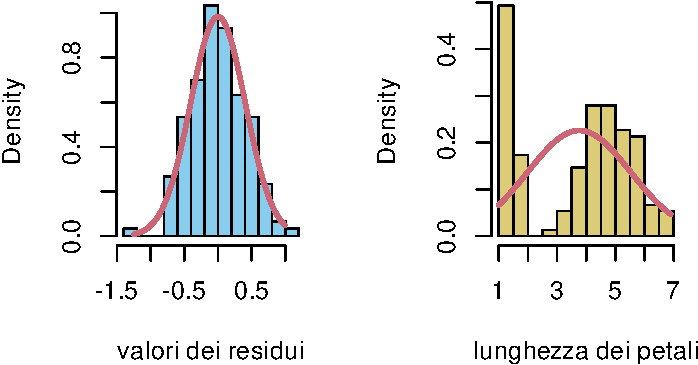
\includegraphics[keepaspectratio]{05-VA_gaussiane_files/figure-pdf/unnamed-chunk-36-1.pdf}}
\end{center}

\begin{Shaded}
\begin{Highlighting}[]
\CommentTok{\# notiamo una buona aderenza dei dati alla densità teorica nel primo caso, e invece una notevole differenza nel secondo.}
\end{Highlighting}
\end{Shaded}

Un secondo metodo grafico è il \emph{Q-Q plot}, in cui si confrontano la
funzione quantile della variabile empirica, ossia la variabile uniforme
discreta sugli \(n\) valori osservati, con la funzione quantile di una
opportuna gaussiana -- in tal caso, l'ipotesi di gaussianità è tanto più
ragionevole quanto più i punti sul grafico siano allineati.

\begin{Shaded}
\begin{Highlighting}[]
\CommentTok{\# per il Q{-}Q plot in R usiamo il comando qqnorm() che automaticamente confronta il quantile della variabile "empirica" con quello di una gaussiana }

\FunctionTok{par}\NormalTok{(}\AttributeTok{mfrow  =} \FunctionTok{c}\NormalTok{(}\DecValTok{1}\NormalTok{,}\DecValTok{2}\NormalTok{))}

\FunctionTok{qqnorm}\NormalTok{(iris\_res, }\AttributeTok{col=}\NormalTok{miei\_colori[}\DecValTok{1}\NormalTok{], }\AttributeTok{pch=}\DecValTok{16}\NormalTok{)}

\CommentTok{\# per aggiungere la linea che si dovrebbe ottenere se l\textquotesingle{}ipotesi fosse vera (per opportuni parametri) usiamo il comando qqline()}

\FunctionTok{qqline}\NormalTok{(iris\_res, }\AttributeTok{col=}\NormalTok{miei\_colori[}\DecValTok{2}\NormalTok{], }\AttributeTok{lwd=}\DecValTok{2}\NormalTok{)}


\CommentTok{\# ripetiamo per la lunghezza dei petali}


\FunctionTok{qqnorm}\NormalTok{(iris\_petali, }\AttributeTok{col=}\NormalTok{miei\_colori[}\DecValTok{3}\NormalTok{], }\AttributeTok{pch=}\DecValTok{16}\NormalTok{)}

\FunctionTok{qqline}\NormalTok{(iris\_petali, }\AttributeTok{col=}\NormalTok{miei\_colori[}\DecValTok{2}\NormalTok{], }\AttributeTok{lwd=}\DecValTok{2}\NormalTok{)}
\end{Highlighting}
\end{Shaded}

\begin{center}
\pandocbounded{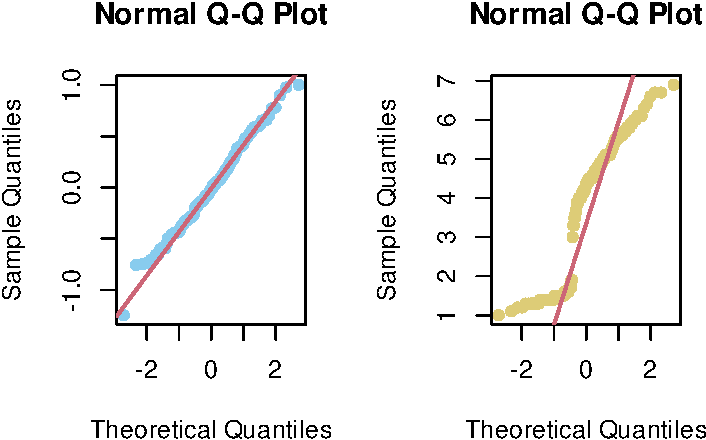
\includegraphics[keepaspectratio]{05-VA_gaussiane_files/figure-pdf/unnamed-chunk-37-1.pdf}}
\end{center}

\begin{Shaded}
\begin{Highlighting}[]
\CommentTok{\# nel primo caso  la maggior parte dei punti è ben allineata alla retta, mentre nel secondo si discostano.}
\end{Highlighting}
\end{Shaded}

\begin{enumerate}
\def\labelenumi{\arabic{enumi}.}
\setcounter{enumi}{1}
\tightlist
\item
  Approcci \emph{quantitativi}: si introducono tuttavia dei \emph{test}
  statistici in cui l'ipotesi nulla è l'evento (o meglio l'unione degli
  eventi al variare dei parametri di media e varianza)
  \(\mathcal{H}_0 =\) ``le osservazioni provengono da \(n\) variabili
  gaussiane indipendenti, tutte con gli stessi parametri'' e
  l'alternativa semplice \(H_1\) è la sua negazione. La descrizione
  specifica di questi test, in particolare dell'evento su cui si basa
  poi la decisione (rifiutare o meno) l'ipotesi nulla è troppo lunga, e
  la omettiamo. Ricordiamo però dal breve cenno ai test nella Sezione
  Sezione~\ref{sec-bayes-stat} che le quantità principali, in
  particolare il valore \(p\), sono calcolate rispetto alla probabilità
  condizionata alla validità dell'ipotesi nulla, pertanto si possono
  calcolare, almeno in linea di principio, perché l'ipotesi nulla
  riguarda densità gaussiane -- il problema in questo caso sarebbe
  l'alternativa in cui non è chiaro quale densità considerare. In ogni
  caso, bisogna comunque prestare attenzione al fatto che un test
  statistico, pur essendo quantitativo non è una ``dimostrazione'' che
  l'ipotesi nulla sia vera (si usa appunto la locuzione \emph{non viene
  rifiutata} per evitare di cadere in questa trappola concettuale).
  Ricordiamo infine che, più piccolo il valore \(p\), maggiore sarà il
  ``grado di fiducia'' che il test attribuisce nel rifiutare l'ipotesi
  nulla, quindi se il motivo per cui utilizziamo un test è di
  confermare, o meglio non smentire, l'ipotesi di gaussianità, il test
  sarà tanto più utile quanto più \emph{grande} (ossia vicino ad \(1\))
  è il valore \(p\). Vediamo degli esempi.
\end{enumerate}

\begin{Shaded}
\begin{Highlighting}[]
\CommentTok{\# Un test di gaussianità è dovuto a Shapiro (e Wilk). }

\FunctionTok{shapiro.test}\NormalTok{(iris\_res)}
\end{Highlighting}
\end{Shaded}

\begin{verbatim}

    Shapiro-Wilk normality test

data:  iris_res
W = 0.99298, p-value = 0.6767
\end{verbatim}

\begin{Shaded}
\begin{Highlighting}[]
\FunctionTok{shapiro.test}\NormalTok{(iris\_petali)}
\end{Highlighting}
\end{Shaded}

\begin{verbatim}

    Shapiro-Wilk normality test

data:  iris_petali
W = 0.87627, p-value = 7.412e-10
\end{verbatim}

\begin{Shaded}
\begin{Highlighting}[]
\CommentTok{\# vediamo come nel caso dei residui il p{-}value sia molto grande (0.67), mentre nel secondo il test rifiuta la gaussianità con un p{-}value estremamente piccolo.}

\CommentTok{\# Un test basato sulla funzione di ripartizione è dovuto a Kolmogorov e Smirnov. In realtà questo è un test che permette di confrontare anche con altre densità, non solo gaussiane, quindi dobbiamo specificare il parametro "pnorm"  per il test di gaussianità (con altri parametri si può testare altre densità).}

\FunctionTok{ks.test}\NormalTok{(iris\_res,  }\StringTok{"pnorm"}\NormalTok{, }\AttributeTok{mean=}\FunctionTok{mean}\NormalTok{(iris\_res), }\AttributeTok{sd=}\FunctionTok{sd}\NormalTok{(iris\_res))}
\end{Highlighting}
\end{Shaded}

\begin{verbatim}

    Asymptotic one-sample Kolmogorov-Smirnov test

data:  iris_res
D = 0.040916, p-value = 0.9632
alternative hypothesis: two-sided
\end{verbatim}

\begin{Shaded}
\begin{Highlighting}[]
\FunctionTok{ks.test}\NormalTok{(iris\_petali,  }\StringTok{"pnorm"}\NormalTok{, }\AttributeTok{mean=}\FunctionTok{mean}\NormalTok{(iris\_petali), }\AttributeTok{sd=}\FunctionTok{sd}\NormalTok{(iris\_petali))}
\end{Highlighting}
\end{Shaded}

\begin{verbatim}

    Asymptotic one-sample Kolmogorov-Smirnov test

data:  iris_petali
D = 0.19815, p-value = 1.532e-05
alternative hypothesis: two-sided
\end{verbatim}

\begin{Shaded}
\begin{Highlighting}[]
\CommentTok{\# anche in questo caso il valore p è estremamente indicativo e conferma quanto osservato qualitativamente.}
\end{Highlighting}
\end{Shaded}

\subsection{Esercizi}\label{esercizi-31}

Si considerino le varie colonne del dataset `mtcars' e si discuta se sia
opportuno supporre che siano osservazioni di variabili gaussiane
indipendenti. Lo stesso per i residui della regressione lineare della
colonna `qsec' rispetto alla colonna `hp'.

\section{Approssimazione di Laplace}\label{sec-laplace}

Concludiamo questo capitolo discutendo un problema leggermente diverso
da quello della sezione precedente, ma in un certo senso collegato: data
una variabile \(X \in \R^d\) di cui sappiamo che la densità non è
gaussiana, in quale senso è possibile comunque approssimarla con una
gaussiana? In questo modo ad esempio gli strumenti sviluppati per le
variabili gaussiane si potrebbero applicare, tenendo conto dell'errore
di approssimazione, anche ad altre densità.

Una soluzione particolarmente semplice e spesso efficace è
l'\textbf{approssimazione di Laplace}, che consiste nello sviluppare al
secondo ordine il logaritmo della densità di \(X\)
\[ x \mapsto \log( p(X=x)),\] (supponendo che \(X\) ammetta una densità
continua e abbastanza regolare), in un punto di massimo \(x_{{\max}}\)
(ossia una moda della densità di \(X\)). Poiché il gradiente si annulla,
si trova lo sviluppo \[ \begin{split} & \log( p(X = x) ) \\
& = \log( p(X= x_{{\max}})) + \frac  12 (x-x_{{\max}}) \cdot  H(x_{{\max}}) (x-x_{{\max}}) + O( |x-x_{{\max}}|^3),
\end{split}\] dove
\[ H(x) = \bra{ \frac{ \partial^2 \log (p(X=x))}{\partial x_i \partial x_j}}_{i,j=1}^d\]
la matrice delle derivate seconde (detta anche hessiana). Essendo
\(x_{{\max}}\) punto di massimo, \(H\) è una matrice (semi-)definita
negativa. Supponendo che sia negativa, allora l'approssimazione di
Laplace è data dalla densità gaussiana di valor medio \(x_{{\max}}\) e
matrice delle covarianze \(- (H(x_{\max}))^{-1}\). L'utilità di questo
metodo è che spesso, nel calcolare \(x_{{\max}}\) tramite opportuni
metodi numerici si calcola anche la matrice hessiana (ad esempio con il
metodo di Newton).

Va evidenziato tuttavia che non è garantita in generale che
l'approssimazione sia vicina alla densità di \(X\), in particolare per
valori \(x\) lontani da \(x_{{\max}}\). Vediamo degli esempi.

\begin{Shaded}
\begin{Highlighting}[]
\CommentTok{\# Iniziamo con una densità non gaussiana ma piuttosto simile, }

\NormalTok{deltax}\OtherTok{=} \FloatTok{0.01}
\NormalTok{x}\OtherTok{=} \FunctionTok{seq}\NormalTok{(}\DecValTok{0}\NormalTok{,}\DecValTok{1}\NormalTok{, }\AttributeTok{by=}\NormalTok{deltax)}

\NormalTok{densita }\OtherTok{=}\NormalTok{ x}\SpecialCharTok{\^{}}\DecValTok{4}\SpecialCharTok{*}\NormalTok{(}\DecValTok{1}\SpecialCharTok{{-}}\NormalTok{x)}\SpecialCharTok{\^{}}\DecValTok{4}
\NormalTok{densita }\OtherTok{=}\NormalTok{ densita}\SpecialCharTok{/}\FunctionTok{sum}\NormalTok{(densita}\SpecialCharTok{*}\NormalTok{deltax)}

\FunctionTok{plot}\NormalTok{(x,densita, }\AttributeTok{type=}\StringTok{\textquotesingle{}l\textquotesingle{}}\NormalTok{, }\AttributeTok{lwd=}\DecValTok{3}\NormalTok{, }\AttributeTok{col=}\NormalTok{miei\_colori[}\DecValTok{1}\NormalTok{], }\AttributeTok{ylab=}\StringTok{\textquotesingle{}densità\textquotesingle{}}\NormalTok{)}

\CommentTok{\# calcoliamo il minimo dell\textquotesingle{}opposto del logaritmo della densità con la funzione nlm() {-}{-} questo si può anche fare a mano, ma poi lo possiamo applicare a casi generali. Dobbiamo comunque specificare la funzione fuori dall\textquotesingle{}intervallo [0,1], ponendola ad esempio infinita.}

\NormalTok{log\_dens }\OtherTok{=} \ControlFlowTok{function}\NormalTok{(x)\{}
  \ControlFlowTok{if}\NormalTok{( x }\SpecialCharTok{\textless{}}\DecValTok{0} \SpecialCharTok{|}\NormalTok{ x}\SpecialCharTok{\textgreater{}} \DecValTok{1}\NormalTok{)}
    \ConstantTok{Inf}
  \ControlFlowTok{else} 
    \SpecialCharTok{{-}}\FunctionTok{log}\NormalTok{( x}\SpecialCharTok{\^{}}\DecValTok{4}\SpecialCharTok{*}\NormalTok{(}\DecValTok{1}\SpecialCharTok{{-}}\NormalTok{x)}\SpecialCharTok{\^{}}\DecValTok{4}\NormalTok{)}
\NormalTok{    \}}

\NormalTok{moda }\OtherTok{=} \FunctionTok{nlm}\NormalTok{( log\_dens, }\AttributeTok{p=}\DecValTok{2}\SpecialCharTok{/}\DecValTok{3}\NormalTok{,  }\AttributeTok{hessian=}\ConstantTok{TRUE}\NormalTok{)}

\CommentTok{\# ricaviamo il punto di massimo e la matrice hessiana (qui la derivata seconda)}

\NormalTok{moda}\SpecialCharTok{$}\NormalTok{estimate}
\end{Highlighting}
\end{Shaded}

\begin{verbatim}
[1] 0.4999995
\end{verbatim}

\begin{Shaded}
\begin{Highlighting}[]
\NormalTok{moda}\SpecialCharTok{$}\NormalTok{hessian}
\end{Highlighting}
\end{Shaded}

\begin{verbatim}
     [,1]
[1,]   32
\end{verbatim}

\begin{Shaded}
\begin{Highlighting}[]
\CommentTok{\# aggiungiamo ora al plot la densità ottenuta con l\textquotesingle{}approssimazione di Laplace}

\FunctionTok{plot}\NormalTok{(x,densita, }\AttributeTok{type=}\StringTok{\textquotesingle{}l\textquotesingle{}}\NormalTok{, }\AttributeTok{lwd=}\DecValTok{3}\NormalTok{, }\AttributeTok{col=}\NormalTok{miei\_colori[}\DecValTok{1}\NormalTok{], }\AttributeTok{ylab=}\StringTok{\textquotesingle{}densità\textquotesingle{}}\NormalTok{)}
\FunctionTok{lines}\NormalTok{(x, }\FunctionTok{dnorm}\NormalTok{(x,}\AttributeTok{mean =}\NormalTok{ moda}\SpecialCharTok{$}\NormalTok{estimate, }\AttributeTok{sd =} \FunctionTok{sqrt}\NormalTok{(}\DecValTok{1}\SpecialCharTok{/}\NormalTok{moda}\SpecialCharTok{$}\NormalTok{hessian) ), }\AttributeTok{lwd=}\DecValTok{3}\NormalTok{, }\AttributeTok{col=}\NormalTok{miei\_colori[}\DecValTok{2}\NormalTok{])}


\FunctionTok{legend}\NormalTok{(}\StringTok{\textquotesingle{}topright\textquotesingle{}}\NormalTok{, }\AttributeTok{legend=}\FunctionTok{c}\NormalTok{(}\StringTok{\textquotesingle{}originale\textquotesingle{}}\NormalTok{,}\StringTok{\textquotesingle{}approssimata\textquotesingle{}}\NormalTok{), }\AttributeTok{fill=}\NormalTok{miei\_colori[}\DecValTok{1}\SpecialCharTok{:}\DecValTok{2}\NormalTok{])}
\end{Highlighting}
\end{Shaded}

\begin{center}
\pandocbounded{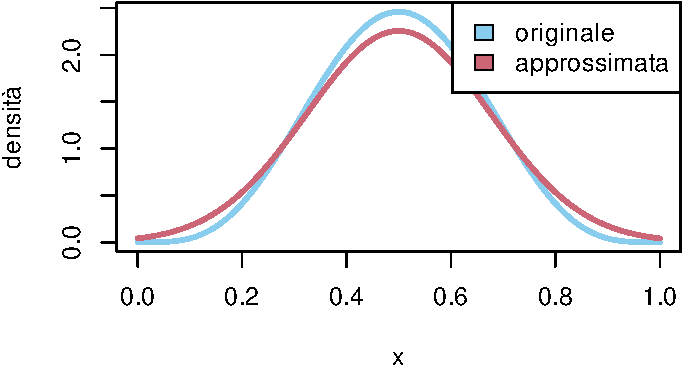
\includegraphics[keepaspectratio]{05-VA_gaussiane_files/figure-pdf/unnamed-chunk-39-1.pdf}}
\end{center}

Basta tuttavia modificare di poco l'esempio sopra per ottenere una
cattiva approssimazione, dovuta all'asimmetria della densità.

\begin{Shaded}
\begin{Highlighting}[]
\NormalTok{densita }\OtherTok{=}\NormalTok{ x}\SpecialCharTok{\^{}}\DecValTok{3}\SpecialCharTok{*}\NormalTok{(}\DecValTok{1}\SpecialCharTok{{-}}\NormalTok{x)}\SpecialCharTok{\^{}}\DecValTok{5}
\NormalTok{densita }\OtherTok{=}\NormalTok{ densita}\SpecialCharTok{/}\FunctionTok{sum}\NormalTok{(densita}\SpecialCharTok{*}\NormalTok{deltax)}


\NormalTok{log\_dens }\OtherTok{=} \ControlFlowTok{function}\NormalTok{(x)\{}
  \ControlFlowTok{if}\NormalTok{ (x}\SpecialCharTok{\textless{}}\DecValTok{0} \SpecialCharTok{|}\NormalTok{ x}\SpecialCharTok{\textgreater{}}\DecValTok{1}\NormalTok{)}
    \ConstantTok{Inf}
  \ControlFlowTok{else}
   \SpecialCharTok{{-}}\FunctionTok{log}\NormalTok{( x}\SpecialCharTok{\^{}}\DecValTok{3}\SpecialCharTok{*}\NormalTok{(}\DecValTok{1}\SpecialCharTok{{-}}\NormalTok{x)}\SpecialCharTok{\^{}}\DecValTok{5}\NormalTok{)}
\NormalTok{    \}}

\NormalTok{moda }\OtherTok{=} \FunctionTok{nlm}\NormalTok{( log\_dens, }\AttributeTok{p=}\DecValTok{1}\SpecialCharTok{/}\DecValTok{2}\NormalTok{, }\AttributeTok{hessian=}\ConstantTok{TRUE}\NormalTok{)}



\FunctionTok{plot}\NormalTok{(x,densita, }\AttributeTok{type=}\StringTok{\textquotesingle{}l\textquotesingle{}}\NormalTok{, }\AttributeTok{lwd=}\DecValTok{3}\NormalTok{, }\AttributeTok{col=}\NormalTok{miei\_colori[}\DecValTok{1}\NormalTok{], }\AttributeTok{ylab=}\StringTok{\textquotesingle{}densità\textquotesingle{}}\NormalTok{)}
\FunctionTok{lines}\NormalTok{(x, }\FunctionTok{dnorm}\NormalTok{(x,}\AttributeTok{mean =}\NormalTok{ moda}\SpecialCharTok{$}\NormalTok{estimate, }\AttributeTok{sd =} \FunctionTok{sqrt}\NormalTok{(}\DecValTok{1}\SpecialCharTok{/}\NormalTok{moda}\SpecialCharTok{$}\NormalTok{hessian) ), }\AttributeTok{lwd=}\DecValTok{3}\NormalTok{, }\AttributeTok{col=}\NormalTok{miei\_colori[}\DecValTok{2}\NormalTok{])}


\FunctionTok{legend}\NormalTok{(}\StringTok{\textquotesingle{}topright\textquotesingle{}}\NormalTok{, }\AttributeTok{legend=}\FunctionTok{c}\NormalTok{(}\StringTok{\textquotesingle{}originale\textquotesingle{}}\NormalTok{,}\StringTok{\textquotesingle{}approssimata\textquotesingle{}}\NormalTok{), }\AttributeTok{fill=}\NormalTok{miei\_colori[}\DecValTok{1}\SpecialCharTok{:}\DecValTok{2}\NormalTok{])}
\end{Highlighting}
\end{Shaded}

\begin{center}
\pandocbounded{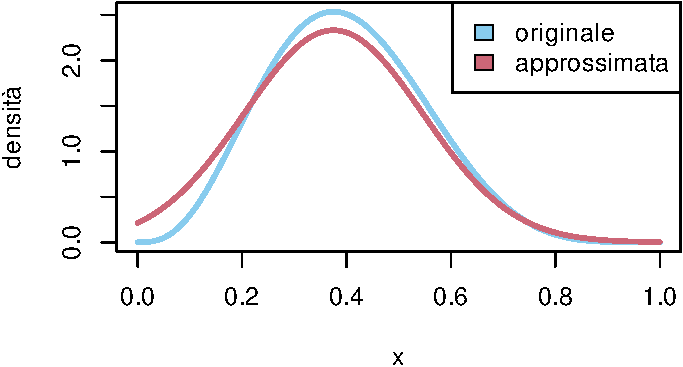
\includegraphics[keepaspectratio]{05-VA_gaussiane_files/figure-pdf/unnamed-chunk-40-1.pdf}}
\end{center}

Nel caso di densità con più di un punto di massimo locale
l'approssimazione è ben peggiore, come è naturale aspettarsi.

\begin{Shaded}
\begin{Highlighting}[]
\NormalTok{x}\OtherTok{=} \FunctionTok{seq}\NormalTok{(}\SpecialCharTok{{-}}\DecValTok{2}\NormalTok{, }\DecValTok{2}\NormalTok{, }\AttributeTok{by=}\NormalTok{deltax)}
\NormalTok{densita }\OtherTok{=} \FunctionTok{exp}\NormalTok{(}\SpecialCharTok{{-}}\NormalTok{(}\DecValTok{1}\SpecialCharTok{{-}}\NormalTok{x)}\SpecialCharTok{\^{}}\DecValTok{2}\SpecialCharTok{*}\NormalTok{(}\DecValTok{1}\SpecialCharTok{+}\NormalTok{x)}\SpecialCharTok{\^{}}\DecValTok{2}\NormalTok{)}
\NormalTok{densita }\OtherTok{=}\NormalTok{ densita}\SpecialCharTok{/}\FunctionTok{sum}\NormalTok{(densita}\SpecialCharTok{*}\NormalTok{deltax)}


\NormalTok{log\_dens }\OtherTok{=} \ControlFlowTok{function}\NormalTok{(x)\{}
  \ControlFlowTok{if}\NormalTok{(x }\SpecialCharTok{\textless{}} \SpecialCharTok{{-}}\DecValTok{2} \SpecialCharTok{|}\NormalTok{ x }\SpecialCharTok{\textgreater{}} \DecValTok{2}\NormalTok{)\{}
    \ConstantTok{Inf}
\NormalTok{  \}}
  \ControlFlowTok{else}
\NormalTok{    (}\DecValTok{1}\SpecialCharTok{{-}}\NormalTok{x)}\SpecialCharTok{\^{}}\DecValTok{2}\SpecialCharTok{*}\NormalTok{(}\DecValTok{1}\SpecialCharTok{+}\NormalTok{x)}\SpecialCharTok{\^{}}\DecValTok{2} 
\NormalTok{  \}}

\NormalTok{moda }\OtherTok{=} \FunctionTok{nlm}\NormalTok{(  log\_dens, }\AttributeTok{p=}\SpecialCharTok{{-}}\FloatTok{1.5}\NormalTok{, }\AttributeTok{hessian=}\ConstantTok{TRUE}\NormalTok{)}



\FunctionTok{plot}\NormalTok{(x,densita, }\AttributeTok{type=}\StringTok{\textquotesingle{}l\textquotesingle{}}\NormalTok{, }\AttributeTok{lwd=}\DecValTok{3}\NormalTok{, }\AttributeTok{col=}\NormalTok{miei\_colori[}\DecValTok{1}\NormalTok{], }\AttributeTok{ylim=}\FunctionTok{c}\NormalTok{(}\DecValTok{0}\NormalTok{,}\FloatTok{1.2}\NormalTok{), }\AttributeTok{ylab=}\StringTok{\textquotesingle{}densità\textquotesingle{}}\NormalTok{)}
\FunctionTok{lines}\NormalTok{(x, }\FunctionTok{dnorm}\NormalTok{(x,}\AttributeTok{mean =}\NormalTok{ moda}\SpecialCharTok{$}\NormalTok{estimate, }\AttributeTok{sd =} \FunctionTok{sqrt}\NormalTok{(}\DecValTok{1}\SpecialCharTok{/}\NormalTok{moda}\SpecialCharTok{$}\NormalTok{hessian) ), }\AttributeTok{lwd=}\DecValTok{3}\NormalTok{, }\AttributeTok{col=}\NormalTok{miei\_colori[}\DecValTok{2}\NormalTok{])}


\FunctionTok{legend}\NormalTok{(}\StringTok{\textquotesingle{}topright\textquotesingle{}}\NormalTok{, }\AttributeTok{legend=}\FunctionTok{c}\NormalTok{(}\StringTok{\textquotesingle{}originale\textquotesingle{}}\NormalTok{,}\StringTok{\textquotesingle{}approssimata\textquotesingle{}}\NormalTok{), }\AttributeTok{fill=}\NormalTok{miei\_colori[}\DecValTok{1}\SpecialCharTok{:}\DecValTok{2}\NormalTok{])}
\end{Highlighting}
\end{Shaded}

\begin{center}
\pandocbounded{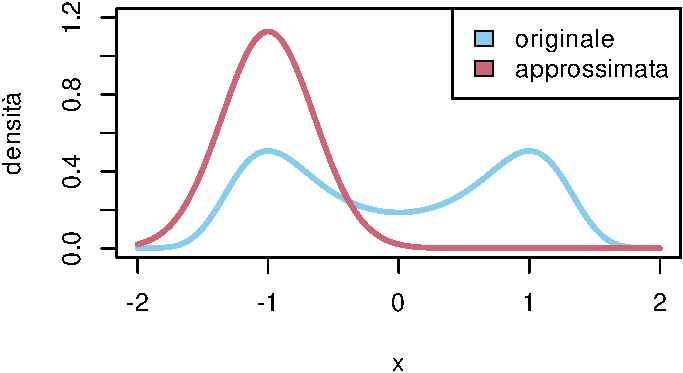
\includegraphics[keepaspectratio]{05-VA_gaussiane_files/figure-pdf/unnamed-chunk-41-1.pdf}}
\end{center}

Consideriamo infine un esempio nel caso vettoriale. Approssimiamo
variabile a valori in \(\R^2\) con densità
\[ p( (X,Y ) = (x,y)) \propto  (5-(y-\sin(2\pi x))^2 )(1-x^2)(1-y^2)\]
per \(x\), \(y \in [-1,1]\) e nulla fuori.

\begin{Shaded}
\begin{Highlighting}[]
\NormalTok{deltax}\OtherTok{=}\FloatTok{0.05}
\NormalTok{deltay}\OtherTok{=}\FloatTok{0.05}

\NormalTok{x}\OtherTok{=} \FunctionTok{seq}\NormalTok{(}\SpecialCharTok{{-}}\DecValTok{1}\NormalTok{,}\DecValTok{1}\NormalTok{, }\AttributeTok{by=}\NormalTok{deltax)}
\NormalTok{y}\OtherTok{=}\FunctionTok{seq}\NormalTok{(}\SpecialCharTok{{-}}\DecValTok{1}\NormalTok{,}\DecValTok{1}\NormalTok{, }\AttributeTok{by=}\NormalTok{deltay)}

\NormalTok{N\_x }\OtherTok{=} \FunctionTok{length}\NormalTok{(x)}
\NormalTok{N\_y }\OtherTok{=} \FunctionTok{length}\NormalTok{(y)}


\CommentTok{\# creiamo una matrice con i valori della densità, inizialmente tutti nulli}

\NormalTok{densita }\OtherTok{=} \FunctionTok{matrix}\NormalTok{(  }\AttributeTok{nrow=}\NormalTok{N\_x, }\AttributeTok{ncol=}\NormalTok{N\_y)}

\CommentTok{\# definiamo la funzione che calcola la densità}

\NormalTok{densita\_funzione }\OtherTok{=} \ControlFlowTok{function}\NormalTok{( v)\{}
\NormalTok{  (}\DecValTok{5}\SpecialCharTok{{-}}\NormalTok{(v[}\DecValTok{2}\NormalTok{]}\SpecialCharTok{{-}}\FunctionTok{sin}\NormalTok{(}\DecValTok{2}\SpecialCharTok{*}\NormalTok{pi}\SpecialCharTok{*}\NormalTok{v[}\DecValTok{1}\NormalTok{]))}\SpecialCharTok{\^{}}\DecValTok{2}\NormalTok{ )}\SpecialCharTok{*}\NormalTok{(}\DecValTok{1}\SpecialCharTok{{-}}\NormalTok{v[}\DecValTok{1}\NormalTok{]}\SpecialCharTok{\^{}}\DecValTok{2}\NormalTok{)}\SpecialCharTok{*}\NormalTok{(}\DecValTok{1}\SpecialCharTok{{-}}\NormalTok{v[}\DecValTok{2}\NormalTok{]}\SpecialCharTok{\^{}}\DecValTok{2}\NormalTok{)}
\NormalTok{\}}

\ControlFlowTok{for}\NormalTok{ (i }\ControlFlowTok{in} \DecValTok{1}\SpecialCharTok{:}\NormalTok{N\_x  )\{}
  \ControlFlowTok{for}\NormalTok{ (j }\ControlFlowTok{in} \DecValTok{1}\SpecialCharTok{:}\NormalTok{N\_y)\{}
\NormalTok{    densita[i,j]}\OtherTok{=} \FunctionTok{densita\_funzione}\NormalTok{( }\FunctionTok{c}\NormalTok{(x[i], y[j]))}
\NormalTok{  \}}
\NormalTok{\}}

\NormalTok{densita }\OtherTok{=}\NormalTok{ densita}\SpecialCharTok{/}\FunctionTok{sum}\NormalTok{(densita}\SpecialCharTok{*}\NormalTok{deltax}\SpecialCharTok{*}\NormalTok{deltay)}



\FunctionTok{filled.contour}\NormalTok{(x, y, densita, }\AttributeTok{color.palette =}\NormalTok{  viridis, }\AttributeTok{xlab=}\StringTok{\textquotesingle{}x\textquotesingle{}}\NormalTok{, }\AttributeTok{ylab=}\StringTok{\textquotesingle{}y\textquotesingle{}}\NormalTok{)}
\end{Highlighting}
\end{Shaded}

\begin{figure}[H]

{\centering \pandocbounded{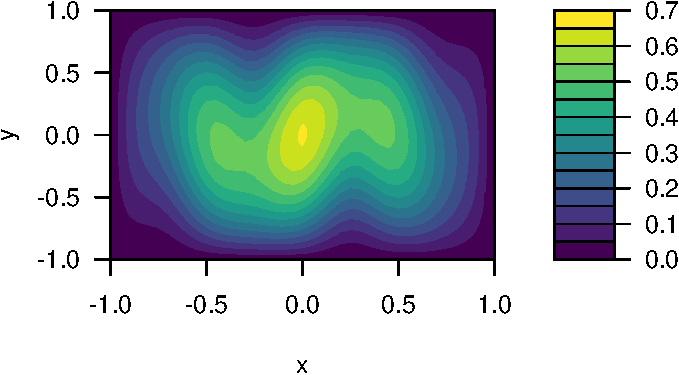
\includegraphics[keepaspectratio]{05-VA_gaussiane_files/figure-pdf/unnamed-chunk-42-1.pdf}}

}

\caption{heatmap della densità sopra}

\end{figure}%

Vediamone ora l'approssimazione di Laplace.

\begin{Shaded}
\begin{Highlighting}[]
\NormalTok{log\_dens }\OtherTok{=} \ControlFlowTok{function}\NormalTok{(x)\{}
  \ControlFlowTok{if}\NormalTok{( }\FunctionTok{abs}\NormalTok{(x[}\DecValTok{1}\NormalTok{])}\SpecialCharTok{\textgreater{}}\DecValTok{1} \SpecialCharTok{|} \FunctionTok{abs}\NormalTok{(x[}\DecValTok{2}\NormalTok{]) }\SpecialCharTok{\textgreater{}} \DecValTok{1}\NormalTok{)\{}
    \ConstantTok{Inf}
\NormalTok{  \}}
  \ControlFlowTok{else}
    \SpecialCharTok{{-}}\FunctionTok{log}\NormalTok{(  }\FunctionTok{densita\_funzione}\NormalTok{(x))}
\NormalTok{  \}}

\NormalTok{moda }\OtherTok{=} \FunctionTok{nlm}\NormalTok{(  log\_dens, }\AttributeTok{p=}\FunctionTok{c}\NormalTok{(}\FloatTok{0.5}\NormalTok{, }\FloatTok{0.5}\NormalTok{), }\AttributeTok{hessian=}\ConstantTok{TRUE}\NormalTok{)}


\FunctionTok{library}\NormalTok{(mvtnorm)}

\NormalTok{m }\OtherTok{=}\NormalTok{ moda}\SpecialCharTok{$}\NormalTok{estimate}

\CommentTok{\# usiamo la funzione solve per calcolare l\textquotesingle{}inversa della matrice hessiana}
\NormalTok{K }\OtherTok{=} \FunctionTok{solve}\NormalTok{(moda}\SpecialCharTok{$}\NormalTok{hessian)}


\ControlFlowTok{for}\NormalTok{ (i }\ControlFlowTok{in} \DecValTok{1}\SpecialCharTok{:}\NormalTok{N\_x  )\{}
  \ControlFlowTok{for}\NormalTok{ (j }\ControlFlowTok{in} \DecValTok{1}\SpecialCharTok{:}\NormalTok{N\_y)\{}
\NormalTok{    densita[i,j]}\OtherTok{=} \FunctionTok{dmvt}\NormalTok{( }\FunctionTok{c}\NormalTok{(x[i], y[j]), m, K)}
\NormalTok{  \}}
\NormalTok{\}}



\FunctionTok{filled.contour}\NormalTok{(x, y, densita, }\AttributeTok{color.palette =}\NormalTok{  viridis, }\AttributeTok{xlab=}\StringTok{\textquotesingle{}x\textquotesingle{}}\NormalTok{, }\AttributeTok{ylab=}\StringTok{\textquotesingle{}y\textquotesingle{}}\NormalTok{)}
\end{Highlighting}
\end{Shaded}

\begin{figure}[H]

{\centering \pandocbounded{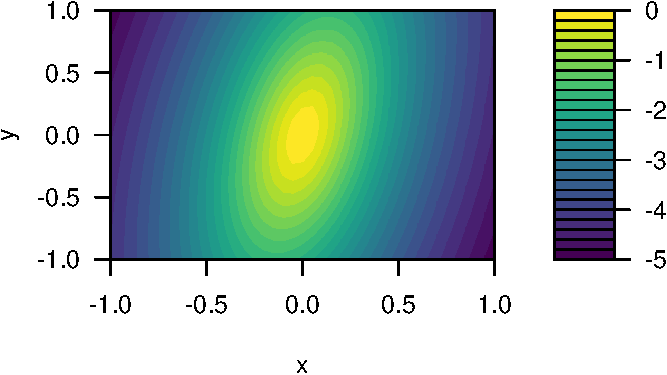
\includegraphics[keepaspectratio]{05-VA_gaussiane_files/figure-pdf/unnamed-chunk-43-1.pdf}}

}

\caption{heatmap dell'approssimazione di Laplace.}

\end{figure}%

\subsection{Esercizi}\label{esercizi-32}

Scrivere l'approssimazione di Laplace per una densità proporzionale a
\(x^3 (1-x)^2\) per \(x \in [0,1]\), e nulla altrimenti. Procedere sia
analiticamente che tramite opportuni comandi R.

\section{Problemi}\label{problemi-3}

\bookmarksetup{startatroot}

\chapter{Processi stocastici a stati discreti}\label{sec-markov}

In questo capitolo iniziamo lo studio generale dei processi stocastici,
concentrandoci nel caso di processi di Markov a stati discreti (catene
di Markov e processi di Markov a salti).

\begin{itemize}
\item
  Nella Sezione Sezione~\ref{sec-definizioni-processi} introduciamo il
  linguaggio di base della teoria con alcune definizioni generali ma
  fondamentali.
\item
  Successivamente, la Sezione Sezione~\ref{sec-catene-markov} e la
  Sezione Sezione~\ref{sec-markov-salti} sviluppano la teoria di base
  rispettivamente delle catene di Markov e dei processi di Markov a
  salti.
\item
  La Sezione Sezione~\ref{sec-invarianti} si occupa delle distribuzioni
  invarianti associate ad un processo di Markov (a stati finiti o
  comunque discreti), discutendone proprietà fondamentali come
  l'esistenza e l'eventuale unicità.
\item
  Le Sezione Sezione~\ref{sec-mle-markov} è dedicata al problema di
  stimare i parametri di un processo di Markov a partire dalla
  osservazione della traiettoria. Discutiamo brevemente la stima di
  massima verosimiglianza con qualche accenno ai metodi bayesiani.
\item
  Concludiamo con la Sezione Sezione~\ref{sec-code} studiando degli
  esempi fondamentali di catene su stati infiniti dalla teoria delle
  code.
\end{itemize}

\section{Definizioni generali}\label{sec-definizioni-processi}

Un \textbf{processo stocastico} è una collezione di variabili aleatorie
\((X_t)_{t \in \mathcal{T}}\), tutte a valori nello stesso insieme
\(E\), detto insieme degli \textbf{stati} del processo, e indicizzate da
un insieme \(\mathcal{T} \subseteq \R\) detto insieme dei \textbf{tempi}
del processo.

Abbiamo già visto in realtà collezioni di variabili aleatorie, ad
esempio nei modelli delle estrazioni da un'urna: basta fare
corrispondere ogni estrazione \(1, 2, 3, \ldots\) ad un opportuno
``istante'' (anche semplicemente \(t=1, 2,3..\)).

Il calcolo delle probabilità fornisce strumenti utili per affrontare
problemi relativi ad affermazioni che riguardano il \emph{futuro} di un
processo (questo è il problema della \emph{previsione}) quanto quelli
riguardanti il \emph{passato}, oppure anche il \emph{presente} (se non è
esattamente osservato, il problema della ricostruzione dello stato
presente è noto come problema del \emph{filtraggio}).

Analogamente alle singole variabili aleatorie, si classificano i
processi stocastici in base al fatto che \(E\) sia discreto (quindi
finito oppure infinito numerabile, ad esempio \(E = \mathbb{Z}\) oppure
\(\N\)), e in tal caso si dice che il processo è a \textbf{stati
discreti}, oppure \(E\) sia infinito continuo, \(E = \R\), \(E = \R^k\)
(e di solito ciascuna \(X_t\) ammetta densità continua), e in tal caso
si dice che il processo è a \textbf{stati continui}.

È possibile anche introdurre una ulteriore classificazione, in base alla
struttura dell'insieme \(\mathcal{T}\) dei tempi: il processo si dice a
\textbf{tempi discreti} se \(\mathcal{T}\) è discreto (ad esempio
finito, oppure \(\mathcal{T} = \N\)), mentre invece se \(E = [0,T]\) è
un intervallo (anche illimitato, ad esempio \(E = [0, \infty)\)), il
processo si dice a \textbf{tempi continui}.

Combinando questi due criteri si definiscono quindi quattro possibili
``classi'' di processi, e noi svilupperemo la teoria per studiare esempi
fondamentali da tre di queste (il caso di tempi e stati continui è
tecnicamente più complicato e non lo tratteremo).

È utile pensare ad un processo stocastico \((X_t)_{t \in \mathcal{T}}\)
come ad una variabile aleatoria vettoriale a valori in uno spazio di
\textbf{traiettorie}, \(E^{\mathcal{T}}\), formalmente lo spazio delle
funzioni dai tempi \(\mathcal{T}\) a valori negli stati \(E\). Ad
esempio, se \(\mathcal{T} = \cur{1, \ldots, d}\), allora un processo
\((X_i)_{i=1}^d\) può essere pensato come una variabile aleatoria
congiunta \(X\), a valori in \(E^d\), l'insieme delle \(d\)-uple
ordinate di elementi di \(E\). È particolarmente importante ricordare
quindi la differenza (valida in generale) tra la legge delle marginali
(rispetto ad una informazione nota \(I\)), ossia tutte le probabilità
del tipo \[ P(X_t \in U|I),\] al variare di \(U \subseteq E\) e
\(t \in \mathcal{T}\), e la legge congiunta, in questo caso detta
semplicemente legge del processo \((X_t)_{t \in \mathcal{T}}\), che è
definita come tutte le probabilità del tipo
\[ P(X_{t_1} \in U_1, X_{t_2} \in U_2, \ldots, X_{t_k} \in U_k | I),\]
al variare di tutte le possibili scelte di tempi \(t_1\), \(t_2\),
\ldots, \(t_k \in \mathcal{T}\), e sottoinsiemi dei possibil valori
\(U_1\), \ldots, \(U_k \subseteq E\), e del numero dei tempi \(k \ge 1\)
(questa definizione permette anche di trattare un numero infinito di
tempi).

Queste definizioni generali, valide sia per stati discreti che continui,
si riformulano nei contesti specifici introducendo le densità (delle
marginali e del processo). Nel caso di processi a stati discreti, per
ogni \(t \in \mathcal{T}\) la densità discreta della marginale al tempo
\(t\), è la funzione che ad \(x \in E\) associa \[ P(X_t = x |I ).\] La
densità discreta del processo è invece la collezione delle probabilità
\[ P(X_{t_1}= x_1, X_{t_2}=x_2, \ldots, X_{t_k} =x_k| I),\] al variare
di tutte le possibili scelte di tempi \(t_1\), \(t_2\), \ldots,
\(t_k \in \mathcal{T}\), e dei possibil valori \(x_1\), \ldots,
\(x_k \in E\), e del numero dei tempi \(k \ge 1\).

Nel caso di processi a stati continui (meglio, con densità contiuna),
basta sostituire la ``\(P\)'' di probabilità con ``\(p\)'' della densità
di probabilità.

In generale, determinare la legge di un processo tramite pochi parametri
è un problema difficile, soprattutto se l'insieme dei tempi diventa
grande (per non parlare del caso infinito): anche se l'insieme degli
stati \(E = \cur{0,1}\) contiene due soli elementi, la densità discreta
di un processo con \(\mathcal{T} = \cur{1, \ldots, d}\) potrebbe essere
una qualsiasi funzione da \(\cur{0,1}^d\) a valori in \([0,1]\) (l'unica
condizione è che la somma su tutti i valori sia \(1\)), quindi sono
necessari circa \(2^d\) ``parametri'' per descriverla. D'altra parte, le
\(d\) densità marginali si ottengono descrivendo \(d\) ``parametri'' (la
probabilità \(P(X_t = 1 |I)\)), oppure anche meno se le leggi sono tutte
uguali -- basta quindi specificare un solo parametro. Non è pensabile
tuttavia di poter ricostruire la densità del processo a partire dalle
densità marginali, eccetto in casi molto particolari, ad esempio se le
variabili marginali \(X_t\) sono indipendenti tra loro. A partire da
queste premesse, lo studio (e le applicazioni) dei processi stocastici
si concentrano pertanto su alcune famiglie particolari che si descrivono
in modo efficate con pochi parametri. In questo capitolo vedremo il caso
dei \textbf{processi di Markov}, più in particolare delle catene di
Markov e dei processi di Markov a salti, in cui il numero dei
``parametri'' necessari per descrivere la legge del processo è
polinomiale (quadratico) nel numero degli stati \(E\), ma le marginali
non sono (necessariamente) tra loro indipendenti, e anzi permettono di
modellizzare tanti fenomeni osservabili nella realtà.

L'ipotesi principale per definire i processi di Markov, è la proprietà
detta appunto di Markov, che si riassume così: \emph{il futuro e il
passato sono condizionatamente indipendenti, noto esattamente il
presente}. Ecco una definizione precisa:

Un processo \((X_t)_{t \in \mathcal{T}}\) è \textbf{di Markov} (o
markoviano) rispetto all'informazione \(I\) se, per ogni \(x \in E\),
\(t \in \mathcal{T}\), le due variabili congiunte relative ai tempi
``passati'' \((X_s)_{s <t}\) e ``futuri'' \((X_r)_{r> t}\) sono
indipendenti, rispetto all'informazione in cui si conosca esattamente il
presente, ossia \(\cur{X_{t} = x}\) (e \(I\)).

Più esplicitamente, se \(A\) è una qualsiasi affermazione che si può
formulare solamente in termini delle variabili \((X_s)_{s <t}\), e \(B\)
è una qualsiasi affermazione che invece riguarda solamente le variabili
\((X_r)_{r> t}\), allora \(A\), \(B\) sono indipendenti rispetto
all'informazione \(\cur{X_t = x}\) ed \(I\):
\[ P(A, B | I, X_t = x) = P(A | I, X_t = x) P( B | I, X_t = x),\] oppure
\[ P(A | I, X_t = x, B) = P(A | I, X_t = x),\] o anche
\[P( B | I, X_t = x, A) = P(B | I, X_t = x).\]

In termini grafici, la proprietà di Markov si traduce in una rete
bayesiana associata al processo \((X_t)_{t \in \mathcal{T}}\) del
seguente tipo:

\begin{figure}[H]

{\centering \pandocbounded{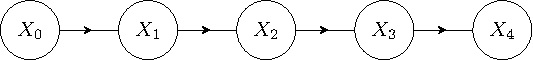
\includegraphics[keepaspectratio]{06-processi_discreti_files/figure-pdf/unnamed-chunk-2-1.pdf}}

}

\caption{Rete bayesiana per un processo di Markov \((X_t)_{t=0}^4\)}

\end{figure}%

Nella definizione di processo di Markov, passato e futuro hanno un ruolo
simmetrico, come è naturale aspettarsi vista la simmetria nel concetto
di indipendenza probabilistica tra due eventi, tuttavia si predilige
spesso il punto di vista in cui si condiziona rispetto al passato e si
calcola la probabilità di un evento futuro.

La proprietà di Markov permette di decomporre la densità (discreta o
continua) del processo in termini di prodotti, usando la regola del
prodotto generalizzata e l'indipendenza: infatti, dati tempi
\(t_1<t_2<\ldots < t_k\) e stati \(x_1\), \ldots{} \(x_k\), si ha
(sottointendendo \(I\))
\begin{equation}\begin{split} & P(X_{t_1}= x_1, X_{t_2}=x_2, \ldots, X_{t_k} =x_k) =\\
& =  P(X_{t_1} = x_1)\cdot  P(X_{t_2}=x_2| X_{t_1} = x_1)
\cdot P(X_{t_3}=x_3| X_{t_2} = x_2, X_{t_1} = x_1)\cdot \ldots \\ 
& \quad \ldots \cdot P( X_{t_k } = x_k | X_{t_{k-1}}=x_{k-1}, \ldots,  X_{t_1} = x_1)\\
& = P(X_{t_1} = x_1) \prod_{i=2}^k P(X_{t_i}=x_i| X_{t_{i-1}} = x_{i-1}). (\#eq:markov-path)\end{split}\end{equation}
Pertanto, per conoscere la densità del processo \(X\), basta conoscere
la densità marginale al tempo \(t_0 = \min \mathcal{T}\) e tutte le
cosiddette \textbf{probabilità di transizione} (o \emph{densità di
transizione} nel caso continuo), ossia \[ P(X_{t } = y | X_s = x),\] al
variare di \(s<t \in \mathcal{T}\) e per ogni coppia di stati \(x\),
\(y \in E\).

Nonostante la notevole semplificazione rispetto alla densità generale,
si tratta comunque di una descrizione complessa (le coppie di tempi
possono essere tantissime, anche infinite). Per procedere ulteriormente
e sviluppare una teoria semplice ma flessibile è opportuno procedere in
due modi:

\begin{enumerate}
\def\labelenumi{\arabic{enumi}.}
\item
  considerare insiemi di tempi \(\mathcal{T}\) come intervalli discreti
  \(\mathcal{T} = \cur{0,1,2,\ldots, n}\) o continui
  \(\mathcal{T} = [0,T]\) (eventualmente anche infiniti). In questo modo
  è sufficiente descrivere la probabilità di transizione tra un istante
  \(s\) e il ``successivo'' \(t =s+1\), nel caso discreto, oppure
  \(t=s+\delta s\) (infinitesimo) nel caso continuo.
\item
  considerare il caso di processi di Markov \textbf{omogenei}, ossia
  tali che le probabilità di transizione dal tempo \(s\) al tempo \(t\)
  dipendano solamente dalla differenza dei tempi \(t-s\), o
  equivalentemente, per ogni \(\Delta t \ge 0\) si abbia
  \[ P(X_{t } = y | X_s = x) = P(X_{t+\Delta t} = y | X_{s+\Delta t } = x)\]
  per stati qualunque \(x\), \(y \in E\), purché \(t+\Delta t\) e
  \(s+\Delta t\) siano pure tempi in \(\mathcal{T}\) (altrimenti non ha
  senso \(X_{t+\Delta t}\) o \(X_{s+\Delta t}\)).
\end{enumerate}

Vedremo nelle prossime sezioni che i processi di Markov che soddisfano
queste due condizioni si possono descrivere con un numero di parametri
dell'ordine degli elementi di \(E\) elevato al quadrato (essenzialmente
tramite una matrice con tante righe e colonne quanti sono gli stati).

\begin{remark}
L'omogeneità riguarda solamente le probabilità di transizione tra stati,
e non la legge marginale al tempo iniziale del processo
\(t_0 = \min\mathcal{T}\). Pertanto per descrivere completamente un
processo di Markov omogeneo bisogna anche specificare tale legge
marginale. Vedremo nelle sezioni successive come le leggi marginali ad
ogni tempo \(t\) si ottengono di conseguenza.
\end{remark}

Concludiamo la sezione con un'ultima definizione molto importante nella
teoria e nelle applicazioni dei un processo stocastici, la
\emph{stazionarietà}. Essa estende in un certo senso l'omogeneità da due
tempi a un numero arbitrario (è tuttavia una definizione generale e non
riguarda solo i processi di Markov).

Un processo \((X_t)_{t \in \mathcal{T}}\) si dice \textbf{stazionario}
se, per ogni \(\Delta t  \ge 0\), la legge (congiunta) del processo
coincide con quella del ``traslato''
\((X_{t+\Delta t})_{ t \in \mathcal{T}}\) (purché i tempi \(t+\Delta t\)
appartengano a \(\mathcal{T}\)). Più precisamente, per ogni \(k\ge 1\) e
\(t_1\), \(t_2\), \ldots, \(t_k \in \mathcal{T}\) e \(\Delta t \ge 0\),
la legge congiunta di \((X_{t_1}, ..., X_{t_k})\) coincide con quella di
\((X_{t_1+\Delta t}, ..., X_{t_k+\Delta t})\), purché i tempi
\(t_i +\Delta t\) appartengano a \(\mathcal{T}\). In particolare, nel
caso di stati discreti, vale
\[ P( X_{t_1}= x_1, \ldots, X_{t_k}= x_k) =  P( X_{t_1+\Delta t }= x_1, \ldots, X_{t_k+\Delta t}= x_k),\]
per qualsiasi scelta di stati \(x_1\), \ldots, \(x_k \in E\). Nel caso
continuo l'identità sopra vale per le densita continue (scrivendo la
densità \(p\) al posto della probabilità \(P\)).

Osserviamo che la stazionarietà implicitamente dipende dall'informazione
che si suppone nota \(I\) (sottointesa sopra).

A volte questa definizione è detta di stazionarietà in senso
\emph{stretto}, per distinguerla da una versione più debole (in senso
lato, si veda la Sezione Sezione~\ref{sec-stazionari-continui}). La
definizione può sembrare macchinosa perché bisogna assicurare che i
tempi traslati \(t_i +\Delta t\) appartengano comunque all'insieme dei
tempi \(\mathcal{T}\). Ma in effetti è una condizione naturale,
altrimenti non avrebbe proprio senso la variabile aleatoria
\(X_{t_i+\Delta t}\). Due casi molto semplici che considereremo spesso
sono i tempi discreti \(\mathcal{T} = \mathbb{N}\), così ponendo
\(\Delta t \in \mathbb{N}\) sicuramente la condizione
\(t_i +\Delta t \in \mathbb{N}\) è sempre soddisfatta, oppure i tempi
continui \(\mathcal{T}= [0, \infty)\). Il vantaggio della definizione
data sopra è che vale anche per insiemi di tempi finiti o comunque
limitati.

\begin{remark}
Se un processo \(X\) è stazionario, necessariamente tutte le leggi delle
marginali \(X_t\) coincidono: basta usare \(k=1\) nella definizione
sopra.
\end{remark}

\subsection{Esercizi}\label{esercizi-33}

Sia \((X_t)_{t\in \mathcal{T}}\) un processo a valori in un inseme di
stati \(E\) discreto, tale che tutte le marginali \(X_t\) siano
indipendenti tra loro. Dire se è markoviano e calcolarne le probabilità
di transizione. Sotto quali condizioni sulle leggi marginali il processo
è stazionario?

\section{Catene di Markov}\label{sec-catene-markov}

In questa sezione studiamo i processi di Markov
\((X_t)_{t \in \mathcal{T}}\) a \emph{tempi discreti}, in particolare
poniamo \[\mathcal{T} = \cur{0,1,2,\ldots, n} \subseteq \mathbb{N}\] e
\emph{stati discreti} (spesso finiti). Per semplificare molti risultati
aggiungeremo anche l'ipotesi che siano processi \emph{omogenei}. In
particolare le \emph{probabilità di transizione} tra \(k\) e
\(k+1 \in \mathcal{T}\) dipendono solo dagli stati \(x\), \(y \in E\), e
non da \(k\): \[ P(X_{k+1} = y | X_k = x) =  P(X_{1} = y| X_0=x).\] La
terminologia più precisa per tali processi è di \textbf{catene di Markov
omogenee} (\emph{homogeneous Markov chains} in inglese) ma spesso
omettiamo per brevità il termine \emph{omogenee} e scriviamo solo catene
di Markov .

\begin{remark}
L'insieme dei tempi \(\mathcal{T}\) non deve necessariamente essere
della forma \(\cur{0,1, \ldots, n}\), ma basta che sia un qualsiasi
``intervallo'' discreto
\(\cur{m, m+1, m+2, \ldots, m+n} \subseteq \mathbb{Z}\) costituito da
tempi equispaziati. Spesso è comodo considerare anche infiniti tempi e
porre direttamente \(\mathcal{T} = \mathbb{N}\) o anche
\(\mathcal{T} = \mathbb{Z}\).
\end{remark}

Le probabilità di transizione \[ Q_{x \to y} = P(X_1 = y | X_0=x)\] al
variare di \(x\), \(y \in E\) sono spesso raccolte in una \emph{matrice}
quadrata, con tante righe e colonne quanti gli stati (eventualmente
infinite), \(Q \in \mathbb{R}^{E \times E}\), detta \emph{matrice di
transizione} associata alla catena di Markov \(X\).

\protect\phantomsection\label{esempio-on-off}
Lo stato di una macchina -- che può essere accesa, \emph{ON}, oppure
spenta, \emph{OFF} -- è rappresentato tramite una catena di Markov
sull'insieme degli stati \(E = \cur{\text{OFF}, \text{ON}}\) con
probabilità di transizione
\[ P(X_1 = \text{ON} | X_0 = \text{OFF}) = 10\%,\]

\[ P(X_1 = \text{OFF} | X_0 = \text{ON}) =70\%.\] Poiché
\[ P(X_1 = \text{OFF} | X_0 = \text{OFF}) = 1- P(X_1 = \text{ON} | X_0 = \text{OFF}) = 90\%,\]
e
\[ P(X_1 = \text{ON} | X_0 = \text{ON}) = 1- P(X_1 = \text{OFF} | X_0 = \text{ON}) = 30\%,\]
possiamo definire la matrice di transizione (ordinando gli stati
nell'ordine \(\text{OFF}\), \(\text{ON}\)) come
\[\bra{ \begin{array}{cc} Q_{\text{OFF} \to \text{OFF}} & Q_{\text{OFF} \to \text{ON}} \\
 Q_{\text{ON} \to \text{OFF}} & Q_{\text{ON} \to \text{ON}} \end{array}} =  \bra{ \begin{array}{cc} 0.9 & 0.1 \\ 0.7 & 0.3 \end{array}}. (\#eq:example-markov-chain)\]

\begin{remark}
Come si può osservare anche nell'Esempio \textbf{?@exm-esempio-on-off},
la somma delle probabilità in ciascuna riga della matrice di transizione
vale \(1\), questo perché, per ogni \(x\in E\), le probabilità
\[ (Q_{x \to y})_{y \in E}  = ( P(X_1 = y| X_0 = x))_{y \in E}\] sono la
densità discreta della variabile \(X_1\) rispetto all'informazione
\(X_0=x\).

In generale, una qualsiasi matrice \(Q\) con entrate a valori in
\([0,1]\) e tale che la somma sulle righe sia costante e uguale ad \(1\)
è detta \textbf{matrice stocastica}. Le matrici di transizione delle
catene di Markov sono tutte matrici stocastiche.

Se anche la somma sulle colonne è uguale ad \(1\) è detta
\textbf{matrice bistocastica} (vedremo l'utilità di questo concetto più
avanti).
\end{remark}

Grazie all'identità \textbf{?@eq-markov-path}, la legge di una catena di
Markov è \emph{determinata} dalla legge marginale al tempo iniziale
(diciamo \(0 \in \mathcal{T}\)) e dalla matrice di transizione. Infatti,
vale
\begin{equation} P(X_0 = x_0, X_1=x_1, \ldots X_n = x_n) = P(X_0 = x_0) \prod_{k=1}^n Q_{x_{k-1}\to x_{k}},  (\#eq:markov-chain-path) \end{equation}
che permette di calcolare la probabilità di osservare che la catena
\(X\) percorra un \textbf{cammino}, ossia una sequenza ordinata di stati
\(\gamma = (x_0 \to x_1 \to \ldots \to x_n)\):
\[ P(X = \gamma) = P(X_0 = x_0) Q_\gamma\] dove il ``peso'' del cammino
\(\gamma\), è il prodotto delle probabilità di transizione
\[ Q_\gamma = \prod_{k=1}^n Q_{x_{k-1}\to x_{k}}.\] Vediamo un esempio.

Si consideri una catena di Markov come nell'Esempio
\textbf{?@exm-esempio-on-off}, con matrice di transizione
\textbf{?@eq-example-markov-chain} e si supponga che valga
\(X_0=\text{OFF}\). Allora la probabilità di osservare il cammino
\[\text{OFF} \to \text{OFF}  \to \text{OFF}  \to \text{ON} \to \text{OFF}  \to \text{ON}\]
è data dal prodotto
\[ 0.9 \cdot 0.9 \cdot 0.1\cdot 0.7\cdot 0.1 = 0.00567.\]

\begin{remark}
Per calcolare la probabilità di una qualsiasi affermazione \(A\) circa
una catena di Markov \((X_n)_{n=0}^\infty\), è quindi sufficiente
rappresentare \(A\) in termini di cammini (a partire dal tempo iniziale)
e sommare le probabilità corrispondenti ottenute tramite la formula
sopra, purché gli eventi relativi a cammini diversi siano a due a due
incompatibili. Questo avviene anche se i cammini hanno lunghezze
diverse, ma \emph{nessun cammino considerato si può ottenere come
prolungamento di un altro}.
\end{remark}

Si consideri una catena di Markov come nell'Esempio
\textbf{?@exm-esempio-on-off}, con matrice di transizione
\textbf{?@eq-example-markov-chain} e \(X_0=\text{OFF}\). Allora la
probabilità
\[ P( \text{$X_2 =\text{OFF}$ oppure $X_3 = \text{ON}$ } ) = 0.916\]
perché l'affermazione sopra equivale ad osservare uno dei seguenti
cammini (a partire dal tempo \(0\) in \(\text{OFF}\))
\[ \begin{array} {|llll|l|} X_0 & X_1 & X_2 & X_3 & Q_\gamma\\
\hline
\text{OFF} & \to \text{OFF} & \to \text{OFF}& & 0.9 \cdot 0.9 \\
   \text{OFF} & \to  \text{ON} &\to \text{OFF}& & 0.1\cdot 0.7\\
    \text{OFF} & \to \text{OFF} &\to \text{ON} & \to \text{ON }& 0.9\cdot 0.1\cdot 0.3\\
    \text{OFF} & \to \text{ON}  & \to \text{ON} & \to  \text{ON}& 0.1\cdot 0.3 \cdot 0.3\\
    \hline
    \end{array}\]

Notiamo che gli eventi corrispondenti sono a due a due incompatibili
perché nessuno dei quattro cammini si ottiene come prolungamento di un
altro. Sommando i pesi dei cammini si ottiene la probabilità cercata.

L'osservazione sopra si giustifica considerando ad esempio la
rappresentazione tramite diagrammi ad albero dei sistemi di alternative
associati a ciascuna variabile \(X_n\) di una catena di Markov. Nella
pratica, tuttavia, tale rappresentazione diventa troppo pesante, e si
preferisce ``comprimerla'' introducendo un grafo pesato orientato i cui
nodi corrispondono agli \emph{stati} \(i \in E\), e l'arco da \(i\) ad
\(j \in E\) è pesato con la probabilità di transizione \(Q_{ij}\) (se la
probabilità è nulla non viene rappresentato). Il grafo associato
permette facilmente di calcolare le probabilità
\[ \prod_{k=1}^n Q_{x_{k-1} x_k}\] associate ad un cammino
\(x_0 \to x_1 \to \ldots \to x_n\), ma non include la probabilità
marginale al tempo \(0\) (necessaria per determinare completamente la
probabilità del cammino).

La rappresentazione grafica di una catena con matrice di transizione
\textbf{?@eq-example-markov-chain} è

\begin{center}
\pandocbounded{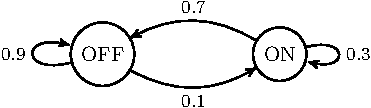
\includegraphics[keepaspectratio]{06-processi_discreti_files/figure-pdf/unnamed-chunk-3-1.pdf}}
\end{center}

Tornando al caso generale, le densità marginali di una catena di Markov
si ottengono sommando la densità congiunta su tutti i possibili valori
delle altre variabili. Pertanto si trova che
\[ P(X_n = x_n) = \sum_{x_0, x_1, \ldots x_{n-1} \in E} P(X_0 = x_0)\prod_{k=1}^n Q_{x_{k-1}x_k}.\]
Per quanto esplicita, la sommatoria sopra è estesa su un grande numero
di valori. Usando direttamente la proprietà di Markov, è possibile
ottenere un'equazione \emph{ricorsiva} per la densità marginale al tempo
\(n\):
\[\begin{split} P(X_n = x_n) & = \sum_{x_{n-1} \in E} P(X_n = x_n | X_{n-1} = x_{n-1}) P(X_{n-1} = x_{n-1})\\
& = \sum_{x_{n-1} \in E} Q_{x_{n-1}x_{n}} P(X_{n-1} = x_{n-1}).\end{split}\]
Se intepretiamo \(Q\) come una matrice in \(\R^{E \times E}\), allora
una densità di probabilità \(P(X_n = \cdot)\) si può pensare come un
vettore in \(\R^{E}\). In particolare, è utile pensarlo come vettore
\emph{riga} \[ \pi_n(x) = P(X_n = x)\] (ossia con tante colonne quante
\(E\)), così la formula sopra diventa semplicemente un prodotto tra
matrici: \[ \pi_{n} = \pi_{n-1} Q, (\#eq:master-discreta)\] che iterando
ci porta ad una versione compatta della formula esplicita sopra:
\[ \pi_n = \pi_{n-1} Q = \pi_{n-2} Q^2 = \ldots = \pi_0 Q^n,\] dove le
potenze \(Q^k\) sono intese nel senso del prodotto di matrici.

In R il prodotto tra matrici (di dimensioni compatibili) si ottiene
tramite il comando \texttt{\%*\%}. Possiamo quindi calcolare e
rappresentare graficamente le densità marginali di una catena avente
matrice di transizione \textbf{?@eq-example-markov-chain} e marginale al
tempo \(0\) uniforme sui due stati.

\begin{Shaded}
\begin{Highlighting}[]
\CommentTok{\# rappresentiamo lo stato iniziale  come un vettore riga}

\NormalTok{dens\_0 }\OtherTok{\textless{}{-}} \FunctionTok{matrix}\NormalTok{( }\FunctionTok{c}\NormalTok{(}\DecValTok{1}\SpecialCharTok{/}\DecValTok{2}\NormalTok{,}\DecValTok{1}\SpecialCharTok{/}\DecValTok{2}\NormalTok{), }\AttributeTok{nrow=}\DecValTok{1}\NormalTok{)}

\CommentTok{\# definiamo la matrice di transizione}

\NormalTok{Q }\OtherTok{=} \FunctionTok{matrix}\NormalTok{( }\FunctionTok{c}\NormalTok{(}\FloatTok{0.9}\NormalTok{, }\FloatTok{0.1}\NormalTok{, }\FloatTok{0.7}\NormalTok{,}\FloatTok{0.3}\NormalTok{ ), }\AttributeTok{nrow=}\DecValTok{2}\NormalTok{, }\AttributeTok{byrow=}\ConstantTok{TRUE}\NormalTok{)}

\CommentTok{\# otteniamo le densità marginali tramite prodotto vettore*matrice}

\NormalTok{dens\_1 }\OtherTok{=}\NormalTok{ dens\_0 }\SpecialCharTok{\%*\%}\NormalTok{ Q}
\NormalTok{dens\_2 }\OtherTok{=}\NormalTok{ dens\_1 }\SpecialCharTok{\%*\%}\NormalTok{ Q}
\NormalTok{dens\_3 }\OtherTok{=}\NormalTok{ dens\_2 }\SpecialCharTok{\%*\%}\NormalTok{ Q}

\CommentTok{\# al solito per rappresentarle in un singolo grafico costruiamo una matrice a partire dalle densità (ciascuna densità è una riga)}

\NormalTok{dens\_matrice }\OtherTok{\textless{}{-}} \FunctionTok{rbind}\NormalTok{(dens\_0, dens\_1, dens\_2, dens\_3)}

\CommentTok{\# Plottiamo il diagramma a barre}

\NormalTok{alternative }\OtherTok{=} \FunctionTok{c}\NormalTok{(}\StringTok{"Off"}\NormalTok{, }\StringTok{"On"}\NormalTok{)}
\NormalTok{colori }\OtherTok{=}\NormalTok{ miei\_colori[}\DecValTok{1}\SpecialCharTok{:}\DecValTok{4}\NormalTok{]}

\FunctionTok{barplot}\NormalTok{( dens\_matrice, }\AttributeTok{beside=}\ConstantTok{TRUE}\NormalTok{, }\AttributeTok{col=}\NormalTok{colori, }\AttributeTok{names.arg=}\NormalTok{alternative, }\AttributeTok{ylab=}\StringTok{"probabilità"}\NormalTok{, }\AttributeTok{xlab=}\StringTok{"stato"}\NormalTok{)}

\CommentTok{\# Aggiungiamo una legenda}

\FunctionTok{legend}\NormalTok{(}\StringTok{\textquotesingle{}topright\textquotesingle{}}\NormalTok{, }\AttributeTok{fill=}\NormalTok{colori, }\AttributeTok{legend=}\FunctionTok{c}\NormalTok{(}\StringTok{"X\_0"}\NormalTok{, }\StringTok{"X\_1"}\NormalTok{, }\StringTok{"X\_2"}\NormalTok{, }\StringTok{"X\_3"}\NormalTok{), }\AttributeTok{cex=}\FloatTok{0.8}\NormalTok{)}
\end{Highlighting}
\end{Shaded}

\begin{figure}[H]

{\centering \pandocbounded{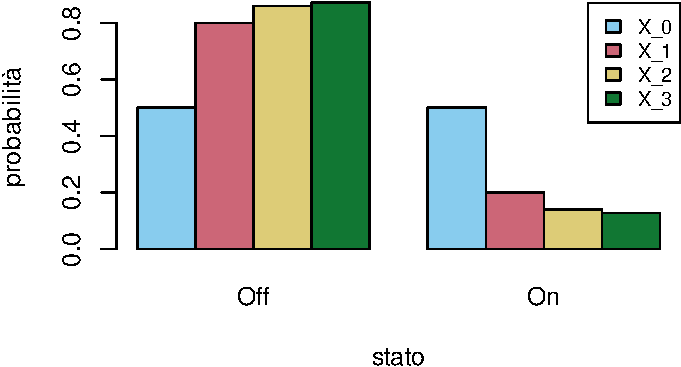
\includegraphics[keepaspectratio]{06-processi_discreti_files/figure-pdf/unnamed-chunk-4-1.pdf}}

}

\caption{Grafico a barre della densità marginale della catena ai tempi
\(0\) (uniforme), \(1\), \(2\) e \(3\).}

\end{figure}%

In alternativa, possiamo rappresentare come funzione del tempo le
densità marginali, come segue:

\begin{Shaded}
\begin{Highlighting}[]
\NormalTok{t }\OtherTok{=} \FunctionTok{seq}\NormalTok{(}\DecValTok{0}\NormalTok{,}\DecValTok{5}\NormalTok{, }\AttributeTok{by=}\DecValTok{1}\NormalTok{)}

\NormalTok{dens }\OtherTok{=}\NormalTok{ dens\_0}
\NormalTok{dens\_matrice }\OtherTok{=}\NormalTok{ dens\_0}

\ControlFlowTok{for}\NormalTok{(iter }\ControlFlowTok{in} \DecValTok{2}\SpecialCharTok{:}\FunctionTok{length}\NormalTok{(t))\{}
\NormalTok{  dens }\OtherTok{=}\NormalTok{ dens }\SpecialCharTok{\%*\%}\NormalTok{ Q}
\NormalTok{  dens\_matrice }\OtherTok{=} \FunctionTok{rbind}\NormalTok{( dens\_matrice, dens)}
\NormalTok{\}}

\FunctionTok{plot}\NormalTok{( t, dens\_matrice[,}\DecValTok{1}\NormalTok{], }\AttributeTok{col=}\NormalTok{miei\_colori[}\DecValTok{1}\NormalTok{], }\AttributeTok{ylim=}\FunctionTok{c}\NormalTok{(}\DecValTok{0}\NormalTok{,}\DecValTok{1}\NormalTok{), }\AttributeTok{ylab=}\StringTok{\textquotesingle{}probabilità\textquotesingle{}}\NormalTok{, }\AttributeTok{type=}\StringTok{\textquotesingle{}l\textquotesingle{}}\NormalTok{, }\AttributeTok{lwd=}\DecValTok{3}\NormalTok{)}
\FunctionTok{lines}\NormalTok{( t, dens\_matrice[,}\DecValTok{2}\NormalTok{], }\AttributeTok{col=}\NormalTok{miei\_colori[}\DecValTok{2}\NormalTok{],}\AttributeTok{type=}\StringTok{\textquotesingle{}l\textquotesingle{}}\NormalTok{, }\AttributeTok{lwd=}\DecValTok{3}\NormalTok{)}



\FunctionTok{legend}\NormalTok{(}\StringTok{\textquotesingle{}topright\textquotesingle{}}\NormalTok{, }\AttributeTok{fill=}\NormalTok{colori, }\AttributeTok{legend=}\FunctionTok{c}\NormalTok{(}\StringTok{"Off"}\NormalTok{,  }\StringTok{"On"}\NormalTok{), }\AttributeTok{cex=}\FloatTok{0.8}\NormalTok{)}
\end{Highlighting}
\end{Shaded}

\begin{figure}[H]

{\centering \pandocbounded{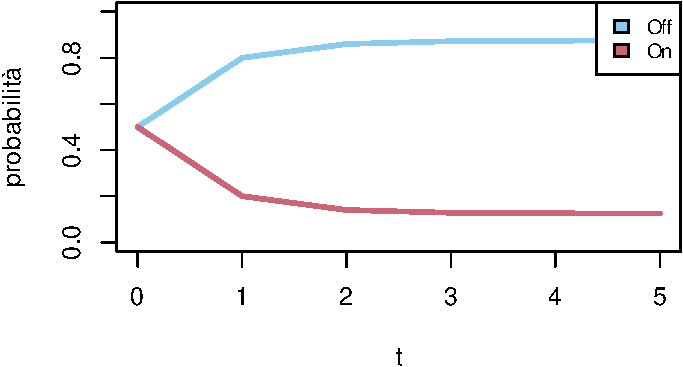
\includegraphics[keepaspectratio]{06-processi_discreti_files/figure-pdf/unnamed-chunk-5-1.pdf}}

}

\caption{grafico delle densità marginali in funzione del tempo
\(t = 0, 1, \ldots, 5\) partendo dalla densità uniforme al tempo \(0\).}

\end{figure}%

Ovviamente le due curve sommano a \(1\) in ogni tempo, ma con più di due
stati è comunque utile rappresentarle tutte.

\subsection{Esercizi}\label{esercizi-34}

Si consideri la matrice \[ Q = \bra{ \begin{array}{lll} 0.1 & 0.3 & * \\
* & 0.5 & 0.4 \\
* & 0.1 & 0.9 
\end{array}}.\] Completare la matrice affinchè sia la matrice di
transizione di una catena di Markov sull'insieme degli stati
\(E = \cur{1,2,3}\). Supponendo che al tempo iniziale \(X_0 = 2\),
calcolare le densità delle marginali ai tempi \(t=1,2,3\) (usare
eventualmente comandi R per semplificare i calcoli) e rappresentare
graficamente tali densità. Calcolare la probabilità dell'evento
``\(X_t \neq 3\) per ogni \(t =1,2,3\)''.

\section{Processi di Markov a salti}\label{sec-markov-salti}

I processi di Markov \((X_t)_{t \in \mathcal{T}}\) a tempi continui
\[\mathcal{T} = [0,T]\] e a stati discreti sono detti \emph{a salti},
perché le traiettorie ``saltano'' da uno stato all'altro -- anche se la
struttura dei tempi permetterebbe un passaggio continuo da uno stato
all'altro, l'insieme degli stati non lo permette.

Come per le catene di Markov, ci limitiamo a considerare il caso di
processi omogenei, ossia tali che, per ogni \(t \in [0,T]\),
\(\delta t>0\) tale che \(t+\delta t \in [0,T]\), si abbia
\[ P(X_{t+\delta t} = y | X_t = x) = P(X_{\delta t} = y| X_0 = x).\] In
analogia con quanto accade per le catene di Markov, per descrivere
completamente la legge di un processo di Markov a salti, è sufficiente
indicare la densità marginale al tempo iniziale
\((P(X_0 = x))_{x\in E}\) e una opportuna matrice che permetta di
determinare le probabilità di transizione da uno stato all'altro. Nel
caso dei processi di Markov a salti, essa è la \textbf{matrice delle
intensità di salto}, definita come
\[ \begin{split} L_{xy} & =\frac{d}{dt}\Bigr|_{\substack{t=0}} P(X_{t} =y| X_0 =x) \\
& =  \lim_{\delta t \to 0}\frac{ P(X_{\delta t} = y | X_0 =x) - P(X_{0} = y | X_0 =x)}{\delta t},\end{split}\]
dove si suppone che il limite esista (finito) per ogni coppia di stati
\(x\), \(y \in E\).

\begin{remark}
La matrice \(L\) si ottiene come derivata della matrice (stocastica)
delle intensità di salto. Pertanto, anche se \(L\) \emph{non} è una
matrice stocastica, essa eredita da questa alcune proprietà: dati \(x\),
\(y \in E\),

\begin{itemize}
\tightlist
\item
  se \(x\neq y\), vale \(P(X_{0} = y | X_0 =x) = 0\) e quindi
  \[ L_{xy} =\frac{d}{dt} P(X_{t} =y| X_0 =x) =  \lim_{\delta t \to 0}\frac{ P(X_{\delta t} = y | X_0 =x)}{\delta t} \ge 0\]
  è una quantità non-negativa (eventualmente nulla), ma non
  necessariamente minore di \(1\)
\item
  se invece \(x=y\), allora \(P(X_0 = y| X_0 = x) = 1\) e quindi
  \[ L_{xy} =\frac{d}{dt} P(X_{t} =y| X_0 =x) =  \lim_{\delta t \to 0}\frac{ P(X_{\delta t} = y | X_0 =x) -1}{\delta t} \le 0.\]
  Infine, la condizione che la somma su ciascuna riga valga \(1\) si
  traduce in
  \[ \sum_{y \in E} L_{xy} = \frac{d}{dt} \sum_{y \in E}  P(X_{t} =y| X_0 =x) = \frac{d}{dt} 1 = 0,\]
  ossia la somma su ciascuna riga vale \(0\), o equivalentemente,
  isolando il termine nella somma in cui \(y=x\),
  \[ L_{xx} = - \sum_{y \neq x} L_{xy}.\]
\end{itemize}

\end{remark}

Lo stato di una macchina può essere spento (Off), in attesa (Standby) o
acceso (On) e lo si modellizza tramite un processo di Markov a salti su
\(E = \cur{\text{Off},  \text{Standby}, \text{On}}\), con matrice delle
intensità di salto \[L  = \bra{ \begin{array}{ccc} * & 5 & 10 \\
 1 & * & 3 \\
 0 & 4 & *
 \end{array}},(\#eq:markov-jump-L)\] dove non abbiamo neppure indicato
le entrate sulla diagonale (che si ricavano imponendo la somma sulle
righe nulla, quindi ad esempio nella prima riga vale \(-15\)).

Il problema che ora affrontiamo è se la matrice delle intensità di salto
sia sufficiente a determinare la legge dell'intero processo (supponendo
anche di conoscere la densità marginale al tempo \(0\)). La risposta è
affermativa, e l'osservazione principale per dedurre risultati analoghi
al caso delle catene di Markov è che i \emph{tempi continui}
\(\mathcal{T} = [0,T]\) possono essere ottenuti come un limite di tempi
discreti
\[ \mathcal{T}^\delta = \cur{0, \delta, 2\delta, \ldots, \lfloor T/ \delta \rfloor \delta },\]
dove \(\lfloor T/\delta \rfloor\) indica il più grande numero naturale
minore di \(T/\delta\). Se si considera il processo ristretto a tali
tempi discreti, ossia si pone \[ X^\delta_k := X_{k \delta},\] esso è
una catena di Markov con matrice di transizione
\[ P^\delta_{xy} = P(X_{\delta} = y| X_0 = x) = Id + L \delta + O(\delta^2) \approx Id + L \delta.\]
Indicando con \(\pi_{t}(x) = P(X_t = x)\) il vettore (riga) della
densità discreta marginale al tempo \(t\), si ha per i tempi della forma
\(t = h \delta\),
\[ \pi_t = \pi_0 ( P^{\delta})^h \approx \pi_0 \bra{ Id + \frac{t L}{h}}^h,\]
avendo scritto \(\delta = t/h\). Ora, fissato \(t \in [0,T]\) si possono
trovare \(h \to \infty\) in modo che \(\delta \to 0\) e quindi,
ricordando il limite notevole (che vale anche per le matrici)
\[ \lim_{h \to \infty} \bra{Id + \frac{A}{h}}^h = \exp\bra{A}, \] si
trova che \[ \pi_t = \pi_0 \exp\bra{ t L}.\] Pertanto, le densità delle
marginali sono determinate dalla matrice \(L\) e dalla densità al tempo
iniziale.

Si consideri un processo di Markov a salti con matrice \(L\) come in
\textbf{?@eq-markov-jump-L}. Supponendo che \(X_0 = \text{Off}\),
possiamo determinare le densità marginali calcolando tramite R
l'esponenziale di matrice (per fare questo è necessario caricare la
libreria \texttt{Matrix} e usare la funzione \texttt{expm()})

\begin{Shaded}
\begin{Highlighting}[]
\CommentTok{\# rappresentiamo lo stato iniziale  come un vettore riga}

\NormalTok{dens\_0 }\OtherTok{\textless{}{-}} \FunctionTok{matrix}\NormalTok{( }\FunctionTok{c}\NormalTok{(}\DecValTok{1}\NormalTok{,}\DecValTok{0}\NormalTok{,}\DecValTok{0}\NormalTok{), }\AttributeTok{nrow=}\DecValTok{1}\NormalTok{)}

\CommentTok{\# definiamo la matrice delle intensità di salto}

\NormalTok{L }\OtherTok{=} \FunctionTok{matrix}\NormalTok{( }\FunctionTok{c}\NormalTok{(}\SpecialCharTok{{-}}\DecValTok{15}\NormalTok{, }\DecValTok{5}\NormalTok{, }\DecValTok{10}\NormalTok{, }\DecValTok{1}\NormalTok{, }\SpecialCharTok{{-}}\DecValTok{4}\NormalTok{, }\DecValTok{3}\NormalTok{, }\DecValTok{0}\NormalTok{, }\DecValTok{4}\NormalTok{, }\SpecialCharTok{{-}}\DecValTok{4}\NormalTok{ ), }\AttributeTok{nrow=}\DecValTok{3}\NormalTok{, }\AttributeTok{byrow=}\ConstantTok{TRUE}\NormalTok{)}

\CommentTok{\# carichiamo la libreria Matrix}

\FunctionTok{library}\NormalTok{(}\StringTok{"Matrix"}\NormalTok{)}

\CommentTok{\# otteniamo le densità marginali tramite prodotto vettore*matrice}

\NormalTok{dens\_01 }\OtherTok{=}\NormalTok{ dens\_0 }\SpecialCharTok{\%*\%} \FunctionTok{expm}\NormalTok{(}\FloatTok{0.1}\SpecialCharTok{*}\NormalTok{L)}
\CommentTok{\# per calcolare la densità al tempo 0.3 possiamo ulteriormente moltiplicare la densità al tempo 0.1 per l\textquotesingle{}esponenziale exp(0.2 L)}
\NormalTok{dens\_03 }\OtherTok{=}\NormalTok{ dens\_01 }\SpecialCharTok{\%*\%}  \FunctionTok{expm}\NormalTok{(}\FloatTok{0.2}\SpecialCharTok{*}\NormalTok{L)}
\NormalTok{dens\_04 }\OtherTok{=}\NormalTok{ dens\_03 }\SpecialCharTok{\%*\%}  \FunctionTok{expm}\NormalTok{(}\FloatTok{0.1}\SpecialCharTok{*}\NormalTok{L)}

\CommentTok{\# al solito per rappresentarle in un singolo grafico costruiamo una matrice a partire dalle densità (ciascuna densità è una riga). È necessario convertire in una matrice perché la libreria Matrix usa un altro oggetto per le matrici {-}{-} e il comando barplot non lo riconosce correttamente}

\NormalTok{dens\_matrice }\OtherTok{\textless{}{-}} \FunctionTok{as.matrix}\NormalTok{(}\FunctionTok{rbind}\NormalTok{(dens\_0, dens\_01, dens\_03, dens\_04))}

\CommentTok{\# Plottiamo il diagramma a barre}

\NormalTok{alternative }\OtherTok{=} \FunctionTok{c}\NormalTok{(}\StringTok{"Off"}\NormalTok{, }\StringTok{"Standby"}\NormalTok{, }\StringTok{"On"}\NormalTok{)}
\NormalTok{colori }\OtherTok{=}\NormalTok{ miei\_colori[}\DecValTok{1}\SpecialCharTok{:}\DecValTok{4}\NormalTok{]}

\FunctionTok{barplot}\NormalTok{( dens\_matrice, }\AttributeTok{beside=}\ConstantTok{TRUE}\NormalTok{, }\AttributeTok{col=}\NormalTok{colori, }\AttributeTok{names.arg=}\NormalTok{alternative, }\AttributeTok{ylab=}\StringTok{"probabilità"}\NormalTok{, }\AttributeTok{xlab=}\StringTok{"stato"}\NormalTok{)}

\CommentTok{\# Aggiungiamo una legenda}

\FunctionTok{legend}\NormalTok{(}\StringTok{\textquotesingle{}topright\textquotesingle{}}\NormalTok{, }\AttributeTok{fill=}\NormalTok{colori, }\AttributeTok{legend=}\FunctionTok{c}\NormalTok{(}\StringTok{"X\_0"}\NormalTok{, }\StringTok{"X\_\{0.1\}"}\NormalTok{, }\StringTok{"X\_\{0.3\}"}\NormalTok{, }\StringTok{"X\_\{0.4\}"}\NormalTok{), }\AttributeTok{cex=}\FloatTok{0.8}\NormalTok{)}
\end{Highlighting}
\end{Shaded}

\begin{figure}[H]

{\centering \pandocbounded{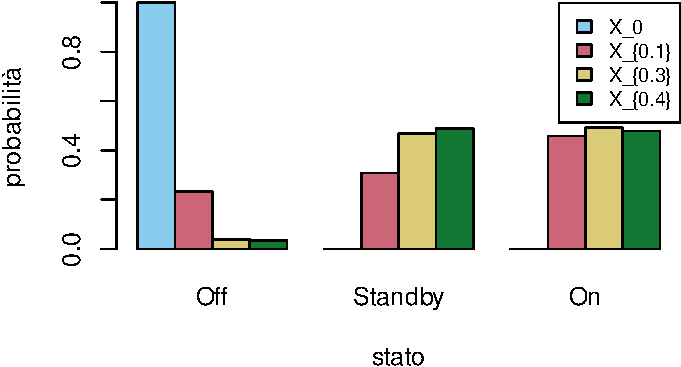
\includegraphics[keepaspectratio]{06-processi_discreti_files/figure-pdf/unnamed-chunk-6-1.pdf}}

}

\caption{Grafico a barre della densità marginale del processo a salti ai
tempi \(0\) (Off), \(0.1\), \(0.3\) e \(0.4\).}

\end{figure}%

\begin{remark}
L'analoga dell'equazione ricorsiva \textbf{?@eq-master-discreta} nel
caso di processi di Markov a salti, è l'equazione differenziale ottenuta
derivando la formula sopra:
\[ \frac{d}{dt} \pi_t = \pi_t L (\#eq:master-continua) \] Tale equazione
\emph{lineare} è detta anche equazione di Kolmogorov (in inglese
\emph{Kolmogorov forward} oppure \emph{master equation}).
\end{remark}

\begin{Shaded}
\begin{Highlighting}[]
\NormalTok{deltat }\OtherTok{=} \FloatTok{0.01}
\NormalTok{t }\OtherTok{=} \FunctionTok{seq}\NormalTok{(}\DecValTok{0}\NormalTok{,}\FloatTok{0.5}\NormalTok{, }\AttributeTok{by=}\NormalTok{deltat)}
\NormalTok{Q}\OtherTok{=} \FunctionTok{as.matrix}\NormalTok{( }\FunctionTok{expm}\NormalTok{(deltat }\SpecialCharTok{*}\NormalTok{L) )}

\NormalTok{dens }\OtherTok{=}\NormalTok{ dens\_0}
\NormalTok{dens\_matrice }\OtherTok{=}\NormalTok{ dens\_0}

\ControlFlowTok{for}\NormalTok{(iter }\ControlFlowTok{in} \DecValTok{2}\SpecialCharTok{:}\FunctionTok{length}\NormalTok{(t))\{}
\NormalTok{  dens }\OtherTok{=}\NormalTok{ dens }\SpecialCharTok{\%*\%}\NormalTok{ Q}
\NormalTok{  dens\_matrice }\OtherTok{=} \FunctionTok{rbind}\NormalTok{( dens\_matrice, dens)}
\NormalTok{\}}

\FunctionTok{plot}\NormalTok{( t, dens\_matrice[,}\DecValTok{1}\NormalTok{], }\AttributeTok{col=}\NormalTok{miei\_colori[}\DecValTok{1}\NormalTok{], }\AttributeTok{ylim=}\FunctionTok{c}\NormalTok{(}\DecValTok{0}\NormalTok{,}\DecValTok{1}\NormalTok{), }\AttributeTok{ylab=}\StringTok{\textquotesingle{}probabilità\textquotesingle{}}\NormalTok{, }\AttributeTok{type=}\StringTok{\textquotesingle{}l\textquotesingle{}}\NormalTok{, }\AttributeTok{lwd=}\DecValTok{3}\NormalTok{)}
\FunctionTok{lines}\NormalTok{( t, dens\_matrice[,}\DecValTok{2}\NormalTok{], }\AttributeTok{col=}\NormalTok{miei\_colori[}\DecValTok{2}\NormalTok{],}\AttributeTok{type=}\StringTok{\textquotesingle{}l\textquotesingle{}}\NormalTok{, }\AttributeTok{lwd=}\DecValTok{3}\NormalTok{)}
\FunctionTok{lines}\NormalTok{( t, dens\_matrice[,}\DecValTok{3}\NormalTok{], }\AttributeTok{col=}\NormalTok{miei\_colori[}\DecValTok{3}\NormalTok{],}\AttributeTok{type=}\StringTok{\textquotesingle{}l\textquotesingle{}}\NormalTok{, }\AttributeTok{lwd=}\DecValTok{3}\NormalTok{)}



\FunctionTok{legend}\NormalTok{(}\StringTok{\textquotesingle{}topright\textquotesingle{}}\NormalTok{, }\AttributeTok{fill=}\NormalTok{colori, }\AttributeTok{legend=}\FunctionTok{c}\NormalTok{(}\StringTok{"Off"}\NormalTok{, }\StringTok{"Standby"}\NormalTok{, }\StringTok{"On"}\NormalTok{), }\AttributeTok{cex=}\FloatTok{0.8}\NormalTok{)}
\end{Highlighting}
\end{Shaded}

\begin{figure}[H]

{\centering \pandocbounded{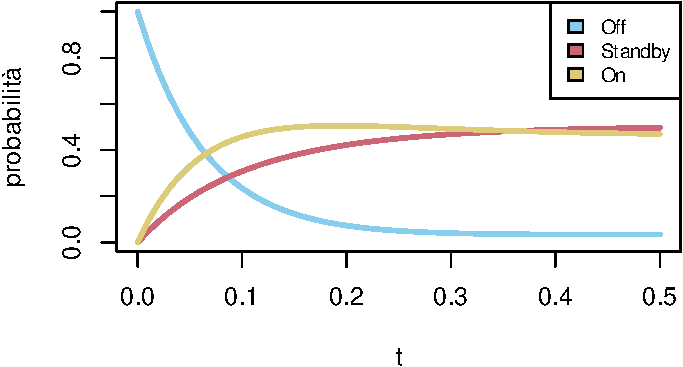
\includegraphics[keepaspectratio]{06-processi_discreti_files/figure-pdf/unnamed-chunk-7-1.pdf}}

}

\caption{grafico delle densità marginali in funzione del tempo
\(t \in [0,0.5]\) partendo dallo stato \(X_0 = \text{Off}\).}

\end{figure}%

Con lo stesso argomento di approssimazione dei tempi continui tramite
tempi discreti, possiamo considerare la probabilità di osservare un
cammino che visiti nell'ordine gli stati
\(x_0 \to x_1 \to \ldots \to x_n\). Trattandosi però di tempi continui,
dobbiamo specificare i \emph{tempi di permanenza} in ciascuno stato
\(t_1,  \ldots, t_n\), in modo che il processo ``salti'' al tempo
\(t_1\) dallo stato \(x_0\) verso \(x_1\), al tempo \(t_1+t_2\) da
\(x_1\) verso \(x_2\), e così via. Fissato \(\delta\) tale che
\(t_1 = \delta h_1\), \(t_2 = \delta h_2\) ecc., si trova
l'approssimazione \[
\begin{split} P( X^\delta = (x_0 \to x_1 \to \ldots \to x_n) )  \approx &  P(X_0 = x_0) (1+ \frac{ t_1 L_{x_{0} x_{0}}}{h_1} )^{h_1} ( \delta L_{x_0 x_1})\cdot \\
& \cdot (1+ \frac{ t_2 L_{x_{1} x_{1}}}{h_2} )^{h_2} ( \delta L_{x_1 x_2})\cdot \ldots\\
& \cdot (1+ \frac{ t_n L_{x_{n-1} x_{n-1}}}{h_n} )^{h_n} ( \delta L_{x_{n-1} x_n}).
\end{split}
\] Al tendere di \(\delta\) a zero si trova che la probabilità tende a
zero: tuttavia dividendo per \(\delta^n\) si ottiene una ``densità'' non
nulla, data dall'espressione
\[ P(X_0 = x_0) \prod_{k=1}^n \exp\bra{t_k L_{x_{k-1} x_{k-1}}} \prod_{k=1}^n L_{x_{k-1} x_k}.\]
L'intepretazione rigorosa si ottiene introducendo le variabili aleatorie
\(T_1\), \(T_2\), \ldots, \(T_n\) che indicando appunto il tempo di
permanenza del processo in ciascuno degli stati visitati \(x_0\),
\(x_1\), \ldots, \(x_{n-1}\). Inoltre, i tempi di salto sono dati dalle
somme \(S_1 = T_1\), \(S_2 = T_1+T_2\), \ldots,
\(S_n = T_1+T_2+\ldots+T_n\). Con questa notazione, abbiamo ottenuto che
\[ \begin{split} p(T_1 = t_1, X_{S_1} & = x_1, T_2 = t_2, X_{S_2} = x_2 \ldots, T_n = t_n, X_{S_n} = x_n) \\
& =  P(X_0 = x_0) \prod_{k=1}^n \exp\bra{t_k L_{x_{k-1} x_{k-1}}}  L_{x_{k-1} x_k},\end{split} (\#eq:likelihood-jump-process)\]
dove la notazione ``\(p\)'' per la densità di probabilità si riferisce
solo alle variabili continue \(T_1\), \(T_2\), \ldots, \(T_n\), mentre
le variabili \(X_{S_1}\), \(X_{S_2}\), \ldots, \(X_{S_n}\) sono
ovviamente discrete (questo è un caso in cui la densità congiunta non è
né discreta né continua). La formula sopra contiene molti prodotti, il
che suggerisce che vi siano variabili indipendenti. In effetti, si può
anche riscrivere in questo modo, separando le variabili continue da
quelle discrete:
\[ P(X_{S_1} = x_1, X_{S_2} = x_2 \ldots,  X_{S_n} = x_n) = P(X_0 =x_0) \prod_{k=1}^n  \frac{ L_{x_{k-1} x_k}}{-L_{x_{k-1} x_{k-1}}},\]
e
\[ \begin{split} & p(T_1 = t_1,  T_2 = t_2, \ldots, T_n = t_n| X_{S_1}= x_1, \ldots  X_{S_n} = x_n) \\
& =  P(X_0 = x_0) \prod_{k=1}^n (-L_{x_{k-1}x_{k-1}}) \exp\bra{t_k L_{x_{k-1} x_{k-1}}}.\end{split}\]
In termini più intuitivi, la prima equazione mostra che le variabili
\(X_0\), \(X_{S_1}\), \ldots, \(X_{S_n}\) che indicano gli stati
visitati dal processo sono una catena di Markov (a tempi discreti) con
probabilità di transizione (per \(x\neq y\))
\[   Q_{xy} = \frac{L_{xy}}{-L_{xx}},\] mentre, supponendo noti gli
stati visitati, i \emph{tempi di permanenza} \(T_1\), \(T_2\), \ldots,
\(T_n\) sono variabili aleatorie indipendenti tra loro, e ciascuna
\(T_k\) ha densità continua esponenziale di parametro
\(-L_{x_{k-1}x_{k-1}}\).

\begin{remark}
Le formule trovate permettono una descrizione alternativa di un processo
di Markov a salti (ad esempio utile per simularli). Una traiettoria del
processo si ottiene a partire da una traiettoria della catena di Markov
con matrice di transizione \(Q\) e successivamente campionando i tempi
di permanenza indipendenti con densità esponenziale dei parametri
opportuni.
\end{remark}

\subsection{Esercizi}\label{esercizi-35}

Si consideri una matrice di intensità di salto (sull'insieme degli stati
\(E = \cur{1,2,3}\)) \[ L = \bra{ \begin{array}{lll} * & 2 & 0 \\
0 & * & 3 \\
1 & 0 & * 
\end{array}}.\] Supponendo che al tempo iniziale sia \(X_0 = 1\),
calcolare le densità delle marginali al tempo \(t=1\) (usare
eventualmente comandi R per semplificare i calcoli) e rappresentare
graficamente tale densità. Si faccia lo stesso (numericamente e
graficamente) per tutti i tempi \(t \in [0,1]\).

\section{Distribuzioni invarianti}\label{sec-invarianti}

Gli esempi delle sezioni precedenti, sia nel caso di catene di Markov
che per processi a salti, mostrano che, partendo da una certa densità
marginale al tempo iniziale, il processo raggiunge (anche piuttosto
rapidamente) un ``equilibrio'' in cui le densità marginali sono costanti
nel tempo. Tale fenomeno è utile in svariate applicazioni, e lo studio
delle possibili densità \emph{limite} è quindi particolarmente
rilevante. Per definire tali densità, basta considerare rispettivamente
l'equazione ricorsiva \textbf{?@eq-master-discreta} o l'equazione
differenziale \textbf{?@eq-master-continua} e imporre che la densità
marginale \emph{non cambi} nel tempo e sia pertanto \emph{invariante}.
Diamo quindi due definizioni, nel caso a tempi discreti (catene) e a
tempi continui (processi a salti).

Sia \(Q\) una matrice di transizione. Si dice che un vettore riga
\(\pi \in \R^E\) corrispondente ad una densità discreta sull'insieme
degli stati, quindi tale che \(\pi_x \in [0,1]\) per ogni \(x \in E\), e
\(\sum_{x \in E} \pi_x = 1\) è una \textbf{distribuzione invariante} per
\(Q\) se vale \[ \pi = \pi Q. (\#eq:inv-Q)\]

Sia \(L\) una matrice di intensità di salto. Si dice che un vettore riga
\(\pi \in \R^E\) corrispondente ad una densità discreta sull'insieme
degli stati, quindi tale che \(\pi_x \in [0,1]\) per ogni \(x \in E\), e
\(\sum_{x \in E} \pi_x = 1\) è una \textbf{distribuzione invariante} per
\(L\) se vale \[ 0 = \pi L. (\#eq:inv-L)\]

\begin{remark}
In entrambi i casi, si può quindi affermare che \(\pi\) è invariante se
e solo se, qualora si consideri un processo \(X\) (catena o a salti)
tale che la legge marginale al tempo iniziale sia \(\pi\), allora tutte
le leggi marginali coincidono con \(\pi\).
\end{remark}

\begin{remark}
La condizione di invarianza si può riscrivere anche come (nel caso delle
catene) segue: per ogni \(x \in E\),
\[ \sum_{y \neq x} \pi_x Q_{x \to y} = \sum_{y \neq x} \pi_y Q_{ y \to x}.\]
In questa formulazione il membro a sinistra si interpreta come flusso
(di probabilità) uscente dallo stato \(x\), mentre il membro a destra è
un flusso entrante. L'equazione esprime quindi un \emph{bilancio di
flusso}. Nel caso di processi a salti, l'equazione diventa
\[ \sum_{y \neq x} \pi_x L_{x  y} = \sum_{y \neq x} \pi_y L_{ yx}.\]
\end{remark}

La seguente proposizione collega il concetto di stazionarietà con il
fatto che la densità delle marginali sia invariante. È ovvio che se la
catena è stazionaria, allora la densità delle marginali deve essere
invariante. Il viceversa richiede qualche osservazione in più, che qui
non riportiamo per brevità.

Sia \(X\) una catena di Markov o un processo di Markov a salti. Allora
\(X\) è stazionario se e solo se la marginale al tempo iniziale \(X_0\)
ha come densità una distribuzione invariante.

La domande teoriche che ci poniamo ora sono: data \(Q\) (oppure \(L\))
le distribuzioni invarianti esistono sempre? se sì, quante sono?

Dal lato pratico è invece importante disporre di algoritmi efficienti
per poter calcolare, almeno in modo approssimato, le distribuzioni
invarianti.

Tali problemi si possono affrontare anche con tecniche di algebra
lineare, perché le equazioni \textbf{?@eq-inv-Q} o \textbf{?@eq-inv-L}
sono dei sistemi di equazioni \emph{lineari} omogenei nelle incognite
date dalle componenti del vettore \(\pi\). In questa sezione ci
limitiamo ad esporre i risultati principali, accennando alle
dimostrazioni.

\subsection{Esistenza}\label{esistenza}

Il primo risultato riguarda l'esistenza di (almeno) una distribuzione
invariante. La risposta è affermativa se l'insieme degli stati \(E\) è
finito.

Se l'insieme degli stati \(E\) è finito, e quindi la matrice di
transizione \(Q\) oppure delle intensità di salto \(L\) sono matrici con
un numero finito di righe e colonne, allora esiste sempre almeno una
distribuzione invariante \(\pi\).

\begin{proof}
Vediamo prima la dimostrazione nel caso delle catene di Markov. Si
consideri una qualsiasi densità discreta \(\pi_0\) sull'insieme degli
stati -- intepretata come vettore riga. Sappiamo che se \(\pi_0\) è la
densità marginale di una catena di Markov \((X_n)_n\) al tempo \(n=0\),
la densità marginale al tempo \(k=0,1,2,\ldots\), è \(\pi_0 Q^k\). Se
esiste il limite per \(k \to \infty\) delle \(\pi_0 Q^k\), esso è una
distribuzione invariante, ma l'esistenza in generale non è garantita
(anzi in generale è falsa). Tuttavia, se si considerano le medie
aritmetiche \[ \bar{\pi}_n = \frac 1 n \sum_{i=1}^n \pi_0 Q^k,\] allora
ciascuna \(\bar{\pi}_n\) è una densità discreta di probabilità (quindi
un vettore a componenti in \([0,1]\) e a somma \(1\)), e per
l'estensione al caso vettoriale del teorema di Bolzano-Weierstrass,
esiste una \emph{sottosuccessione} \(\bar{\pi}_{n_k}\) con
\(n_k \to \infty\) che converge ad un limite
\[ \bar{\pi}_\infty = \lim_{k \to \infty} \bar{\pi}_{n_k},\] ossia tale
che ogni componente del vettore \(\bar{\pi}_{n_k}\) converge alla
corrispondente componente di \(\bar{\pi}_\infty\). Anche il limite è una
densità discreta di probabilità sugli stati \(E\), perché ciascuna
componente del vettore è in \([0,1]\), essendo limiti di valori compresi
tra \(0\) e \(1\), e la somma dei limiti delle componenti coincide con
il limite della somma, che vale \(1\) (qui si usa che \(E\) è finito,
quindi la somma non è una serie). Quindi, basta dimostrare che vale
\[ \bar{\pi}_\infty = \bar{\pi}_\infty Q.\] Per ogni \(n\), si ha
l'identità
\[ \begin{split} \bar{\pi}_n Q & = \bra{ \frac 1 n \sum_{k=1}^n \pi_0 Q^k} Q \\
& = \frac 1 n \sum_{k=1}^n \pi_0 Q^{k+1} \\
& = \frac{1}{n}\sum_{k=1}^n \pi_0 Q^{k} + \frac{1}{n}\bra{ \pi_0 Q^{n+1} - \pi_0 Q}\\
& = \bar{\pi}_n + \frac{1}{n}\bra{ \pi_0 Q^{n+1} - \pi_0 Q}.\end{split}\]
Al tendere di \(n \to \infty\), il termine
\[  \frac{1}{n}\bra{ \pi_0 Q^{n+1} - \pi_0 Q} \to 0\] è infinitesimo al
tendere di \(n \to \infty\), perché le componenti del vettore
\(\pi_0 Q^{n+1}\) sono comprese tra \([0,1]\), e si divide per \(n\).
Ponendo \(n = n_k \to \infty\), concludiamo quindi che
\(\bar{\pi}_\infty\) è una distribuzione invariante.

Nel caso di processi di Markov a salti, l'idea è analoga, ma si
sostituisce alla media aritmetica una media integrale sui tempi, ponendo
\[ \bar{\pi}_t = \frac 1 t \int_0^t \pi_0 \exp\bra{ s L} d s. \] Si può
estrarre anche in questo caso una successione \(t_k\to \infty\) in modo
che \(\bar{\pi}_{t_k}\) converga a un vettore \(\bar{\pi}_\infty\), che
è una densità discreta su \(E\). Per mostrare che è invariante, si
calcola
\[ \begin{split} \bar{\pi}_t L & = \frac 1 t \int_0^t \pi_0 \exp\bra{ s L} L  d s\\
& = \frac 1 t \int_0^t \pi_0 \frac{d}{ds} \exp\bra{ s L}   d s \\
& =  \frac 1 t  \pi_0 \int_0^t \frac{d}{ds} \exp\bra{ s L}   d s\\
& = \frac 1 t \pi_0 \bra{ \exp\bra{t L} - Id},\end{split}\] che al
tendere di \(t \to \infty\) tende a zero (si noti l'analogia con il caso
a tempi discreto).
\end{proof}

Questo risultato teorico garantisce quindi che i sistemi lineari
\textbf{?@eq-inv-Q} o \textbf{?@eq-inv-L} ammettano almeno una
soluzione, e pertanto è sufficiente usare un qualsiasi metodo risolutivo
per determinarla (ad esempio la riduzione a gradini di Gauss). Tuttavia,
la dimostrazione stessa suggerisce un metodo approssimato basato sul
calcolo delle medie \(\bar{\pi}_n\) nel caso di catene o
\(\bar{\pi}_{t}\) nel caso di processi di Markov a salti.

Si consideri la matrice \(Q\) definita in
\textbf{?@eq-example-markov-chain}. Per risolvere il sistema omogeneo,
conviene passare alla trasposta e determinare tutti i vettori colonna
\(x \in \R^2\) tali che \[ (Id - Q^T) x = 0.\] Nel caso di interesse, si
trova che sono tutti del tipo \[ x = u (7,1 )\] dove \(u \in \R\) è un
parametro da determinare imponendo che la somma delle componenti di
\(x\) sia \(1\). Concludendo si trova quindi \(u=8\) e quindi
\[ \pi = (\frac 7 8, \frac 1 8 ).\] Vediamo come procedere tramite R.
Diamo prima una soluzione ``esatta'' mediante il comando
\texttt{eigen()}, che determina autovalori e autovettori: in questo caso
ci interessano infatti gli autovettori di \(Q^T\) con autovalore \(1\),
o equivalentemente gli autovettori di \(Id - Q^T\) con autovalore \(0\)
(il nucleo di \(Id - Q^T\)).

\begin{Shaded}
\begin{Highlighting}[]
\NormalTok{Q }\OtherTok{=} \FunctionTok{matrix}\NormalTok{( }\FunctionTok{c}\NormalTok{(}\FloatTok{0.9}\NormalTok{, }\FloatTok{0.1}\NormalTok{, }\FloatTok{0.7}\NormalTok{,}\FloatTok{0.3}\NormalTok{ ), }\AttributeTok{nrow=}\DecValTok{2}\NormalTok{, }\AttributeTok{byrow=}\ConstantTok{TRUE}\NormalTok{)}

\CommentTok{\#calcoliamo autovalori e autovettori della matrice Q trasposta}

\NormalTok{sol }\OtherTok{=} \FunctionTok{eigen}\NormalTok{(}\FunctionTok{t}\NormalTok{(Q))}

\NormalTok{sol}\SpecialCharTok{$}\NormalTok{values}
\end{Highlighting}
\end{Shaded}

\begin{verbatim}
[1] 1.0 0.2
\end{verbatim}

\begin{Shaded}
\begin{Highlighting}[]
\NormalTok{sol}\SpecialCharTok{$}\NormalTok{vectors}
\end{Highlighting}
\end{Shaded}

\begin{verbatim}
          [,1]       [,2]
[1,] 0.9899495 -0.7071068
[2,] 0.1414214  0.7071068
\end{verbatim}

\begin{Shaded}
\begin{Highlighting}[]
\CommentTok{\# siamo interessati all\textquotesingle{}autovettore di autovalore 1 che è il primo}

\NormalTok{pi\_inv }\OtherTok{=}\NormalTok{ sol}\SpecialCharTok{$}\NormalTok{vectors[, }\DecValTok{1}\NormalTok{]}
\NormalTok{pi\_inv }\OtherTok{=}\NormalTok{ pi\_inv}\SpecialCharTok{/}\FunctionTok{sum}\NormalTok{(pi\_inv)}

\CommentTok{\# la distribuzione invariante è quindi}

\NormalTok{pi\_inv}
\end{Highlighting}
\end{Shaded}

\begin{verbatim}
[1] 0.875 0.125
\end{verbatim}

\begin{Shaded}
\begin{Highlighting}[]
\CommentTok{\# rappresentiamola con un barplot}

\NormalTok{alternative }\OtherTok{=} \FunctionTok{c}\NormalTok{(}\StringTok{"OFF"}\NormalTok{, }\StringTok{"ON"}\NormalTok{)}
\NormalTok{colori }\OtherTok{=}\NormalTok{ miei\_colori[}\DecValTok{1}\NormalTok{]}

\FunctionTok{barplot}\NormalTok{( pi\_inv, }\AttributeTok{col=}\NormalTok{colori, }\AttributeTok{names.arg=}\NormalTok{alternative, }\AttributeTok{ylab=}\StringTok{"probabilità"}\NormalTok{, }\AttributeTok{xlab=}\StringTok{"stato"}\NormalTok{)}
\end{Highlighting}
\end{Shaded}

\begin{center}
\pandocbounded{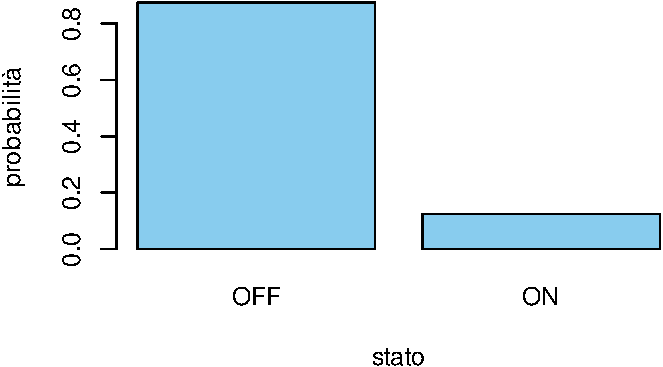
\includegraphics[keepaspectratio]{06-processi_discreti_files/figure-pdf/unnamed-chunk-8-1.pdf}}
\end{center}

Determiniamo le distribuzioni invarianti nel caso della matrice di
intensità di salto \textbf{?@eq-markov-jump-L}.

\begin{Shaded}
\begin{Highlighting}[]
\NormalTok{L }\OtherTok{=} \FunctionTok{matrix}\NormalTok{( }\FunctionTok{c}\NormalTok{(}\SpecialCharTok{{-}}\DecValTok{15}\NormalTok{, }\DecValTok{5}\NormalTok{, }\DecValTok{10}\NormalTok{, }\DecValTok{1}\NormalTok{, }\SpecialCharTok{{-}}\DecValTok{4}\NormalTok{, }\DecValTok{3}\NormalTok{, }\DecValTok{0}\NormalTok{, }\DecValTok{4}\NormalTok{, }\SpecialCharTok{{-}}\DecValTok{4}\NormalTok{ ), }\AttributeTok{nrow=}\DecValTok{3}\NormalTok{, }\AttributeTok{byrow=}\ConstantTok{TRUE}\NormalTok{)}


\NormalTok{sol }\OtherTok{=} \FunctionTok{eigen}\NormalTok{(}\FunctionTok{t}\NormalTok{(L))}

\NormalTok{sol}\SpecialCharTok{$}\NormalTok{values}
\end{Highlighting}
\end{Shaded}

\begin{verbatim}
[1] -1.514005e+01 -7.859945e+00  8.881784e-16
\end{verbatim}

\begin{Shaded}
\begin{Highlighting}[]
\NormalTok{sol}\SpecialCharTok{$}\NormalTok{vectors}
\end{Highlighting}
\end{Shaded}

\begin{verbatim}
           [,1]        [,2]        [,3]
[1,]  0.7539667 -0.09196364 -0.04908437
[2,] -0.1055968 -0.65662548 -0.73626560
[3,] -0.6483699  0.74858912 -0.67491013
\end{verbatim}

\begin{Shaded}
\begin{Highlighting}[]
\CommentTok{\# siamo interessati all\textquotesingle{}autovettore di autovalore 0, che è il terzo}

\NormalTok{pi\_inv }\OtherTok{=}\NormalTok{ sol}\SpecialCharTok{$}\NormalTok{vectors[,}\DecValTok{3}\NormalTok{]}
\NormalTok{pi\_inv }\OtherTok{=}\NormalTok{ pi\_inv}\SpecialCharTok{/}\FunctionTok{sum}\NormalTok{(pi\_inv)}

\CommentTok{\# la distribuzione invariante è quindi}

\NormalTok{pi\_inv}
\end{Highlighting}
\end{Shaded}

\begin{verbatim}
[1] 0.03361345 0.50420168 0.46218487
\end{verbatim}

\begin{Shaded}
\begin{Highlighting}[]
\CommentTok{\# rappresentiamola con un barplot}

\NormalTok{alternative }\OtherTok{=} \FunctionTok{c}\NormalTok{(}\StringTok{"Off"}\NormalTok{, }\StringTok{"Standby"}\NormalTok{, }\StringTok{"On"}\NormalTok{)}
\NormalTok{colori }\OtherTok{=}\NormalTok{ miei\_colori[}\DecValTok{1}\NormalTok{]}

\FunctionTok{barplot}\NormalTok{( pi\_inv, }\AttributeTok{col=}\NormalTok{colori, }\AttributeTok{names.arg=}\NormalTok{alternative, }\AttributeTok{ylab=}\StringTok{"probabilità"}\NormalTok{, }\AttributeTok{xlab=}\StringTok{"stato"}\NormalTok{)}
\end{Highlighting}
\end{Shaded}

\begin{center}
\pandocbounded{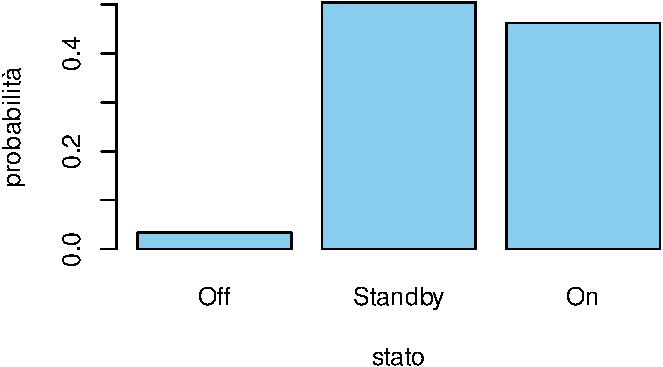
\includegraphics[keepaspectratio]{06-processi_discreti_files/figure-pdf/unnamed-chunk-9-1.pdf}}
\end{center}

\begin{remark}
È fondamentale non confondere l'equazione \(\pi (Id - Q) = 0\), oppure
\(\pi L = 0\) con le ``trasposte'' \((Id - Q) v = 0\) e \(L v = 0\).
Infatti queste hanno sempre come soluzione la densità uniforme
\(v_x = 1/n\), dove \(n\) è il numero degli elementi di \(E\). Questo
perché la somma su ciascuna riga delle matrici di transizione vale \(1\)
(mentre vale \(0\) nel caso delle matrici di intensità di salto).

Se non si specifica l'operazione di trasposizione si trova sempre tale
soluzione, che però non è quella cercata.

Vi è tuttavia un caso in cui la densità uniforme è sicuramente una
distribuzione invariante: si tratta del caso in cui la matrice \(Q\) sia
\emph{bistocastica}, ossia anche la somma sulle colonne dia \(1\). Un
caso particolare è quando \(Q\) sia simmetrica.
\end{remark}

L'potesi che l'insieme degli stati \(E\) sia finito è necessaria. Si
consideri una catena sugli stati \(E = \mathbb{N}\) e
\(Q_{x \to x+1} = 1\) per ogni \(x \in \mathbb{N}\) e \(0\) altrimenti.
Allora ogni distribuzione invariante deve essere uniforme, ma essendo
gli stati infiniti una tale distribuzione non esiste.

\subsection{Unicità}\label{unicituxe0}

Affrontiamo il problema dell'unicità, mostrando in quali condizioni la
distribuzione invariante è unica e che è possibile classificare tutte le
distribuzioni invarianti associate ad una matrice (di transizione \(Q\)
oppure di intensità di salto \(L\)). Cominciamo da un esempio:

\protect\phantomsection\label{alice-bruno}
Un gioco tra Alice e Bruno consiste nel lanciare un dado a sei facce
ripetutamente fintanto che non esca il numero \(1\) (e in tal caso vince
Alice) oppure il numero \(6\) (e e in tal caso vince Bruno). Possiamo
rappresentare una partita tramite una catena di Markov sugli stati
\(E = \cur{A, G, B}\), dove \(A\) indica che Alice ha vinto, \(B\) Bob
ha vinto, e \(G\) il gioco continua (si deve lanciare nuovamente il
dado).

\begin{figure}[H]

{\centering \pandocbounded{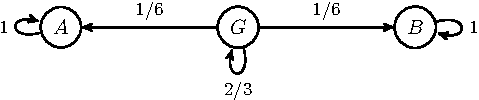
\includegraphics[keepaspectratio]{06-processi_discreti_files/figure-pdf/unnamed-chunk-10-1.pdf}}

}

\caption{Rappresentazione grafica del gioco tra Alice e Bruno}

\end{figure}%

È chiaro che vi sono almeno due distribuzioni stazionarie,
corrispondenti rispettivamente al caso in cui Alice vinca,
\(\pi_A = (1,0,0)\) oppure Bruno vinca, \(\pi_B = (0,0,1)\). Ma in
realtà sono infinite, perché ogni combinazione
\[ \alpha \pi_A + (1-\alpha) \pi_B = (\alpha, 0, 1-\alpha),\quad \text{con $\alpha \in [0,1]$}\]
è pure una distribuzione invariante (corrispondente al fatto che Alice
vinca con probabilità \(\alpha\) e Bob con probabilità \(1-\alpha\)). In
effetti, è intuitivamente chiaro che, se la catena di Markov al tempo
iniziale si trova in \(G\), la densità limite è quella corrispondente ad
\(\alpha = 1/2\), perché le regole del gioco non favoriscono né Alice né
Bruno.

L'esempio sopra evidenzia un fatto generale: se vi sono almeno due
distribuzioni invarianti (diverse), allora le distribuzioni invarianti
sono infinite perché tutte le combinazioni come sopra, al variare del
parametro \(\alpha\in [0,1]\) sono pure invarianti. Se l'insieme degli
stati \(E\) è finito, è possibile determinare un numero finito di
distribuzioni invarianti ``di base'' in modo da poter rappresentare
tutte le altre distribuzioni invarianti come combinazioni di esse. La
procedura è ``geometrica'' e si basa sulla decomposizione dell'insieme
degli stati in sottoinsiemi più piccoli, dette \emph{classi
irriducibili}. Diamo alcune definizioni.

Data una matrice di transizione \(Q\), si dice che lo stato \(y \in E\)
è \textbf{accessibile} (o raggiungibile) da \(x \in E\) se esiste un
cammino \(\gamma = (x_0 \to x_1 \to \ldots \to x_n)\) con \(x_0 = x\) e
\(x_n = y\) e peso strettamente positivo:
\[ Q_\gamma = \prod_{k=1}^n Q_{x_{k-1} x_k} >0. \] Nel caso di una
matrice di intensità di salto \(L\), il peso \(Q_\gamma\) va sostituito
con \[ L_\gamma =  \prod_{k=1}^n L_{x_{k-1} x_k}.\]

Ricordando che \(Q^n_{xy}\) è la somma dei pesi di tutti i cammini
lunghi \(n\) che collegano \(x\) a \(y\), si può equivalentemente dire
che \(y\) è raggiungibile da \(x\) se esiste \(n \ge 1\) tale che
\(Q^n_{xy}>0\).

Osserviamo che \(y \in E\) è raggiungibile da \(x\in E\), e \(z \in E\)
è raggiungibile da \(y\), allora \(z\) è raggiungibile da \(x\).
Tuttavia non è detto che \(x\) sia raggiungibile da \(y\) (o da \(z\)):
se questo appunto non accade, lo stato \(x\) è detto
\textbf{transitorio}.

Data una matrice di transizione \(Q\) (o una matrice di intensità di
salto \(L\)) uno stato \(x \in E\) è detto transitorio se esiste
\(y \in E\) tale che \(y\) è raggiungibile da \(x\), ma \(x\) non lo è
da \(y\). Se \(x\) non è transitorio, è detto \textbf{ricorrente}.

Equivalentemente, \(x\) è ricorrente se, per ogni \(y\in E\) tale che
\(y\) è raggiungibile da \(x\), anche \(x\) lo è da \(y\). Se l'insieme
degli stati \(E\) è finito, non possono essere tutti transitori e deve
esserci almeno uno stato ricorrente.

\protect\phantomsection\label{esempio-catena-due-classi}
Consideriamo una catena di Markov di cui rappresentiamo graficamente la
matrice di transizione come segue (completare per esercizio le
probabilità mancanti, in modo che la somma sulle righe, ossia gli archi
uscenti da ciascuno stato, sia \(1\)):

\begin{center}
\pandocbounded{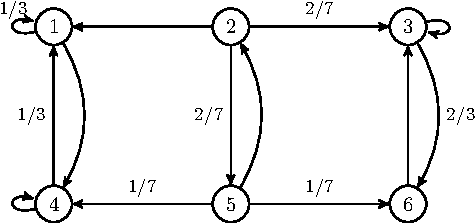
\includegraphics[keepaspectratio]{06-processi_discreti_files/figure-pdf/unnamed-chunk-11-1.pdf}}
\end{center}

Allora stato \(1\) è raggiungibile dallo stato \(2\), mentre lo stato
\(2\) non è raggiungibile dallo stato \(1\). Lo stato \(2\) è quindi
transitorio. Anche lo stato \(5\) lo è. Tutti i rimanenti stati
\(\cur{1,3,4,6}\) sono ricorrenti.

Introduciamo ora il concetto di classe chiusa irriducibile.

Data una matrice di transizione \(Q\) (o una matrice di intensità di
salto \(L\)), un sottoinsieme \(C \subseteq E\) di stati è detto
\textbf{classe chiusa} se, per ogni \(x \in C\) e \(y \in E\)
raggiungibile da \(x\), anche \(y \in C\). Una classe chiusa \(C\) è
detta irriducibile se non contiene altre classi chiuse
\(C' \subseteq C\) (diverse dai casi banali \(C' = \emptyset\) oppure
\(C' = C\) stessa). La matrice \(Q\) (oppure \(L\)) è detta
\textbf{irriducibile} se tutto l'insieme degli stati \(E\) è una classe
chiusa irriducibile.

Equivalentemente, da uno stato in una classe chiusa non è possibile
raggiungere stati al di fuori di essa (mentre è possibile entrarvi), e
una classe chiusa è irriducibile quando da ogni stato in essa si può
raggiungere qualsiasi altro stato in essa. Data una classe chiusa è ben
definita la \emph{restrizione} della matrice \(Q\) su \(C \times C\),
perché \(Q_{x \to y}=0\) per \(x \in C\) e \(y \notin C\), e quindi
\((Q_{x \to y})_{y \in C}\) sono densità discrete di probabilità (la
somma delle righe vale ancora \(1\)). Un ragionamento analogo vale nel
caso di matrici di intensità di salto \(L\).

Riprendiamo l'Esempio \textbf{?@exm-esempio-catena-due-classi}. Gli
stati \(\cur{1,4}\) sono una classe chiusa (irriducibile), mentre ad
esempio gli stati \(\cur{1,2}\) non lo sono, perché si può ``uscirne''
visitando ad esempio lo stato \(4\).

L'importanza della condizione di irreducibilità è dovuta del seguente
risultato.

Sia \(Q\) una matrice di transizione (oppure \(L\) di intensità di
salto) irriducibile su un insieme di stati \(E\) finito. Allora esiste
una e una sola distribuzione invariante.

\begin{proof}
Abbiamo già visto che almeno una distribuzione invariante \(\pi\)
esiste, quindi basta mostrare l'unicità. Nel caso di matrice \(Q\) di
transizione, introduciamo la matrice
\[  R = \frac 1 2 \sum_{n=0}^\infty 2^{-n} Q^n,\] che è pure una matrice
di transizione, in particolare la somma sulle righe vale \(1\) perché
\[ \frac 1 2 \sum_{n=0}^\infty 2^{-n} = 1.\] Grazie all'ipotesi di
irriducibilità è tale che \(R_{xy}>0\) per ogni \(x\), \(y \in E\). Nel
caso di \(L\) matrice di intensità di salto, introduciamo invece
\(R = \exp(L)\) che pure è una matrice di transizione e similmente ha
tutte entrate strettamente positive. Se \(\pi\) è una distribuzione
invariante per \(Q\) (o per \(L\)), vale l'identità
\[ \pi R  = \frac 1 2 \sum_{n=0}^\infty 2^{-n}  \pi Q^ n =  \pi \frac  1 2 \sum_{n=0}^\infty 2^{-n} = \pi,\],
ossia \(\pi\) è distribuzione invariante anche per la matrice di
transizione \(R\) (nel caso di Markov a salti il ragionamento è anche
più semplice). Consideriamo quindi una seconda distribuzione invariante
\(\tilde{\pi}\) e per mostrare che \(\pi = \tilde \pi\) scriviamo la
seguente diseguaglianza:
\[\begin{split} \sum_{x \in E} | \pi_x - \tilde \pi_x| & = \sum_{x \in E}  | \sum_{y \in E} \pi_y R_{yx} - \sum_{y \in E} \tilde \pi_y R_{yx}| \\
& = \sum_{x \in E}  | \sum_{y \in E} (\pi_y - \tilde \pi_y) R_{yx} | \\
& \le \sum_{x \in E} \sum_{y \in E} | \pi_y-\tilde \pi_y| R_{yx} \\
& =  \sum_{y \in E} | \pi_y-\tilde \pi_y| \sum_{x \in E} R_{yx} \\
& = \sum_{y \in E} | \pi_y-\tilde \pi_y|.\end{split}\] Poiché la prima e
l'ultima espressione coincidono (è solamente cambiato l'indice di
somma), devono essere tutte uguaglianze, in particolare nel passaggio in
cui si è stimato, per ogni \(x \in E\),
\[ | \sum_{y \in E} (\pi_y - \tilde \pi_y) R_{yx} | \le \sum_{y \in E} | \pi_y-\tilde \pi_y| R_{yx}\]
deve in realtà valere l'uguaglianza. È noto tuttavia che la
diseguaglianza triangolare tra numeri reali
\[ | \sum_i z_i | \le \sum_i |z_i|\] è una uguaglianza se e solo se
hanno tutti lo stesso segno, ossia \(z_i \ge 0\) per ogni \(i\) oppure
\(z_i \le 0\) per ogni \(i\). Se quindi vale per ogni \(y \in E\)
\[ (\pi_y - \tilde \pi_y )R_{yx} \ge 0,\] essendo \(R_{yx}>0\) si
ottiene (dividendo) che \(\pi_y \ge \tilde \pi_y\) per ogni \(y \in E\).
Ma poiché sono entrambe densità di probabilità,
\[ \sum_{y \in E} \pi _y = 1 = \sum_{y \in E}\tilde{\pi}_y,\] ne segue
che deve valere \(\pi_y = \tilde \pi_y\) (se la diseguaglianza fosse
stretta per qualche \(y\) allora non potrebbe valere l'uguaglianza nella
somma).
\end{proof}

\begin{remark}
La diseguaglianza principale nella dimostrazione sopra si può usare per
mostrare anche che, data una qualsiasi densità discreta \(\pi_0\) su
\(E\) la quantità detta \emph{variazione totale} tra \(\pi_0 Q^n\) e la
distribuzione invariante \(\pi\), \[ \sum_{x\in E} | \pi - \pi_0 Q^n |\]
decresce al crescere di \(n\). Questa è una quantità utile per stimare
la convergenza delle densità marginali di una catena verso la
distribuzione invariante.
\end{remark}

Nel caso in cui \(Q\) non sia irriducibile, bisogna preliminarmente
decomporre \(E\) in classi chiuse irriducibili. Precisamente, ogni
classe chiusa irriducibile non contiene stati transitori (intuitvamente
basterebbe infatti rimuoverli per ottenere una classe chiusa più
piccola), e due classi chiuse irriducibili diverse sono necessariamente
disgiunte (altrimenti l'intersezione sarebbe più piccola di entrambe).
Ne segue che, se \(E\) è finito, si può partizionare in insiemi a due a
due disgiunti
\[ E = \cur{\text{stati transitori}} \cup C^1 \cup C^2 \cup \ldots \cup C^k,\]
dove le \(C^i\) sono classi chiuse irriducibili (\(k \ge 1\) perché non
tutti gli stati sono transitori).

Se consideriamo la restrizione di \(Q\) su ciascuna classe chiusa
irriducibile \(C^i\), allora esiste una e una sola distribuzione
invariante associata \(\pi^i\), che può essere vista come una
distribuzione invariante su tutto l'insieme degli stati \(E\)
(semplicemente la probabilità assegnata al di fuori di \(C^i\) è nulla).
Si può dimostrare (non lo faremo) che \textbf{tutte} le distribuzioni
invarianti sono ottenibili come combinazioni
\[ \pi = \alpha_1 \pi^1 + \alpha_2 \pi^2 + \ldots, + \alpha_k \pi^k,\]
dove \(\alpha_1\), \(\alpha_2\), \ldots, \(\alpha_k \in [0,1]\) sono
tali che \[\alpha_1+\alpha_2 +\ldots + \alpha_k = 1,\] ossia
\((\alpha_i)_{i=1}^k\) sono una (qualsiasi) densità discreta di
probabilità. In particolare, ogni distribuzione invariante è nulla sugli
stati transitori (che quindi si possono subito trascurare se in un
problema è richiesto di calcolare tutte le distribuzioni invarianti).

Riprendiamo l'Esempio \textbf{?@exm-esempio-catena-due-classi}. Per
determinare tutte le distribuzioni invarianti, basta calcolare l'unica
distribuzione per la classe chiusa irriducibile \(C_1 = \cur{1,4}\), che
si trova impostando il bilancio di flusso, ad esempio in \(1\):
\[ \pi_1 \frac 2 3 = \pi_4 \frac  1 3 \quad \text{da cui} \quad (\pi_1, \pi_4) = (\frac 1 3 , \frac 2 3 ).\]
Similmente, per la classe chiusa irriducibile \(C_2 = \cur{3,6}\), si
trova
\[ \pi_3 \frac 2 3 =  \pi_6 \quad \text{da cui} \quad (\pi_3, \pi_6) = (\frac 3 5, \frac 2 5).\]
Di conseguenza tutte le distribuzioni invariante della catena originaria
sono parametrizzate nel seguente modo:
\[ (\alpha \frac 1 3, 0, (1-\alpha) \frac 3 5, \alpha \frac 2 3, 0, (1-\alpha)\frac 2 5 ),\]
dove \(\alpha \in [0,1]\) è un parametro (invece di usare \(2\)
parametri \(\alpha_1\), \(\alpha_2\) che sommano a \(1\) ne indichiamo
solo uno).

\subsection{Sul limite delle potenze della matrice di
transizione}\label{sul-limite-delle-potenze-della-matrice-di-transizione}

In questa sezione, principalmente utile per svolgere alcuni esercizi,
analizziamo più nel dettaglio sotto quali condizioni, data una catena di
Markov\footnote{ci limitiamo al caso delle catene perché è l'unico che
  interviene negli esercizi, per i processi a salti in realtà il
  problema è anche più semplice} con matrice di tranzione \(Q\) su un
insieme di stati finito, il limite \[ \lim_{n \to \infty} (Q^n)_{ij}\]
esiste per ogni coppia di stati \(i\), \(j \in E\). Inoltre presentiamo
un metodo per calcolare tale limite mediante sistemi di equazioni
lineari.

Osserviamo che l'intepretazione di \((Q^n)_{ij}\) in termini di
probabilità è, per via del risultato generale sulle densità marginali,
ponendo \(\pi_0\) la densità discreta che vale \(1\) nello stato \(i\) e
\(0\) altrimenti, \[ (Q^n)_{ij} = P(X_n = j | X_0 =i).\] D'altra parte
le potenze \(Q^n\) intervengono sia nel teorema di esistenza delle
distribuzioni invarianti, sia nel teorema di unicità (un po'
implicitamente, nelle ipotesi per via della condizione di
irriducibilità, e nella dimostrazione per la costruzione della matrice
\(R\), con tutte le entrate positive).

L'osservazione di base è che, se il limite esiste,
\[ Q^\infty_{ij} = \lim_{n \to \infty} (Q^n)_{ij},\] allora è una
matrice le cui righe, ossia i vettori \((Q^\infty_{ij})_{j \in E}\),
sono tutte distribuzioni invarianti. Infatti vale
\[ \begin{split} Q^\infty & = \lim_{n \to \infty }Q^n = \lim_{n \to \infty } Q^{n+1} = \lim_{n \to \infty }Q^n \cdot Q\\
& = Q^\infty\cdot  Q.\end{split}\] Che scritta componente per componente
diventa il sistema definente le distribuzioni invarianti:
\[ Q^\infty_{ij} = \sum_{k} Q^{\infty}_{ik} Q_{k j}.\] Inoltre poiché le
righe di \(Q^n\) sono densità discrete di probabilità, anche il limite
lo è.

Si potrebbe pensare che, se la catena è irriducibile, quindi esiste una
sola distribuzione invariante \(\pi\), allora necessariamente il limite
\(Q^\infty\) esiste ed è la matrice in cui tutte le righe sono identiche
e uguali a \(\pi\). Il ragionamento è corretto, \emph{purché il limite
esista}, cosa che non accade sempre, come il prossimo esempio mostra.

Sia \(E = \cur{\text{Off}, \text{On}}\) e sia (ordinando gli stati
nell'ordine in cui sono scritti),
\[ Q = \bra{ \begin{array}{cc} 0 & 1 \\ 1 & 0 \end{array}}.\] Il grafo
associato è il seguente:

\begin{center}
\pandocbounded{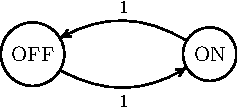
\includegraphics[keepaspectratio]{06-processi_discreti_files/figure-pdf/unnamed-chunk-12-1.pdf}}
\end{center}

La ``dinamica'' della catena è molto semplice: se inizia nello stato
Off, allora passerà a tempi alterni da Off in On. Questo si vede anche
calcolando le potenze di \(Q\),
\[ Q^2 = \bra{ \begin{array}{cc} 1 & 0 \\ 0 & 1 \end{array}} = Id \quad  Q^3 = \bra{ \begin{array}{cc} 0 & 1 \\ 1 & 0 \end{array}}= Q, \quad  Q^4 = Id\ldots\]
quindi il limite \(Q^\infty\) non esiste perché le componenti si
alternano tra i valori \(0\) e \(1\). In questo esempio tuttavia è
facile vedere che la catena è irriducibile con l'unica distribuzione
invariante (uniforme).

La condizione di irriducibilità non è quindi sufficiente a garantire che
il limite \(Q^\infty\) esista. La seguente nozione è invece il concetto
corretto.

Sia \(Q\) una matrice di transizione di una catena di Markov su un
insieme \(E\) di stati finito. Diciamo che \(Q\) (o la catena) è
\textbf{regolare} se esiste \(n\in \mathbb{N}\) tale che la potenza
\(Q^n\) ha tutte entrate strettamente positive, ossia
\[ (Q^n)_{ij} >0 \quad \text{per ogni $i$, $j \in E$.}\]

La definizione somiglia molto a quella di catena irriducibile, ma a ben
vedere è diversa: nel caso di catena irriducibile si richiede che per
ogni \(i\), \(j \in E\) esista un cammino di una qualsiasi lunghezza
\(n\) che li collega, ossia \((Q^n)_{ij}>0\). Nel caso di catena
regolare, si richiede che la lunghezza \(n\) sia la stessa per tutti gli
\(i\), \(j \in E\) (anche quando \(i=j\)). Questo ragionamento ci dice
quindi che \emph{se la catena è regolare, allora è anche irriducibile}.
Ma non necessariamente il viceversa, come mostra l'esempio di prima.

L'importanza del concetto è data dal seguente teorema, che non
dimostriamo, ma è utile negli esercizi.

Sia \(Q\) una matrice di transizione \emph{irriducibile} su un insieme
di stati \(E\) finito. Allora \(Q\) è regolare \emph{se e solo se}
esiste il limite
\[ Q^\infty_{ij} = \lim_{n \to \infty}(Q^{n})_{ij} \quad \text{per ogni $i$, $j \in E$.}\]
Più in generale, anche se \(Q\) non è irriducibile, il limite esiste
(per ogni \(i\), \(j \in E\)) \emph{se e solo se} la catena ristretta a
ciascuna classe chiusa irriducibile è regolare.

Appoggiandosi a questo risultato possiamo garantire l'esistenza di
\(Q^\infty\) in molti problemi concreti: basta prima classificare gli
stati e le classi chiuse irridicubili e controllare che la matrice
ristretta a ciascuna classe sia regolare.

Ci sono però due aspetti pratici da non sottovalutare: come verificare
che \(Q\) sia regolare? Una strategia è di moltiplicare \(Q\) per se
stessa, finché le componenti non sono tutte positive. Un metodo più
semplice è di considerare solo le potenze di \(2\), ossia calcolare
\[Q^2 = Q \cdot Q, \quad Q^4 = Q^2 \cdot Q^2, \quad Q^8 = Q^4\cdot Q^4, \quad \text{ecc.,}\]
In questo modo l'esponente \(n\) cresce più rapidamente e l'algoritmo
termina prima (se termina). Senza un calcolatore, tuttavia tale
algoritmo non è molto pratico. Ci sono però diversi criteri per la
regolarità, e suggeriamo il seguente (senza dimostrazione) che può
essere utile negli esercizi.

Sia \(Q\) una matrice di transizione \emph{irriducibile} su un insieme
di stati \(E\) finito. Se esiste (almeno) uno stato \(i\in E\) tale che
\(Q_{ii}>0\), allora \(Q\) è anche \emph{regolare}.

Basta quindi osservare, dopo aver controllato che \(Q\) sia
irriducibile, che la diagonale della matrice \(Q\) non sia identicamente
nulla. Attenzione tuttavia, la condizione è solo \emph{sufficiente},
esistono catene \(Q\) irriducibili con diagonale tutta nulla ma comunque
regolari. Questo criterio comunque risolve la maggior parte dei casi
concreti (in particolare negli esercizi).

Appurato quindi che \(Q^\infty\) esista (oppure ignorando il problema
temporaneamente), la domanda successiva è come calcolarlo.
L'osservazione chiave è di ripartire dall'argomento che mostrava tutte
le righe invarianti, e trovare una seconda equazione (o sistema di
equazioni):

\[ \begin{split} Q^\infty & = \lim_{n \to \infty }Q^n = \lim_{n \to \infty } Q^{1+n} = \lim_{n \to \infty }Q\cdot Q^n\\
& = Q \cdot Q^\infty.\end{split}\]

Scrivendo la relazione per ciascun elemento della matrice, diventano le
equazioni
\[ Q^{\infty}_{ij} = \sum_{k\in E} Q_{ik} Q^\infty_{kj}, \quad \text{per $i$, $j\in E$.}\]

Queste equazioni, aggiunte all'informazione che le righe di \(Q^\infty\)
sono distribuzioni invarianti, permettono di ottenere un sistema che,
una volta risolto, determina completamente la matrice \(Q^\infty\).

Riprendiamo l'Esempio \textbf{?@exm-alice-bruno} del gioco tra Alice e
Bruno. Sappiamo che tutte le distribuzioni invarianti sono della forma
\((\alpha, 0, 1-\alpha)\), con \(\alpha \in [0,1]\). È ovvio che se lo
stato iniziale della catena è \(A\) (vince Alice), che corrisponde ad
\(\alpha = 1\), allora la catena rimane in quello stato (è assorbente),
e quindi la riga corrispondente nella matrice \(Q^\infty\) è
\[(Q^\infty_{A A}, Q^\infty_{AG}, Q^\infty_{AB}) = (1,0,0).\]
Similmente, se lo stato iniziale è \(B\),
\[(Q^\infty_{B A}, Q^\infty_{BG}, Q^\infty_{BB}) = (0,0,1).\] Resta da
determinare la riga corrispondente allo stato iniziale transitorio
\(G\). Abbiamo già osservato che per simmetria della situazione deve
essere \(\alpha =1/2\), però possiamo anche procedere scrivendo le
equazioni sopra (non serve scriverle tutte, basta trovarne una che
permetta di determinare \(\alpha\)). Ad esempio con \(i= G\), \(j=A\),
troviamo
\[ \begin{split} \alpha & = Q^\infty_{GA} = Q_{GA}Q^{\infty}_{AA} + Q_{GG}Q^{\infty}_{GA} + Q_{GB}Q^{\infty}_{BA}\\
&= \frac 1 6 \cdot 1 + \frac 4 6 \cdot \alpha + \frac 1 6 \cdot 0\end{split}\]
dove abbiamo usato le righe di \(Q^\infty\) precedentemente calcolate
(quelle relative agli stati \(A\) e \(B\)). Concludiamo che
\(\alpha = \frac 1 2\) come avevamo già osservato.

\begin{remark}
Esiste in realtà una formula generale per determinare \(Q^\infty\).
Tuttavia per ottenerla conviene effettuare un passaggio intermedio per
semplificare la struttura della catena e riportarsi in un certo senso
all'esempio sopra, in cui gli stati sono o transitori o assorbenti.

A meno di scegliere opportunamente un ordinamento degli stati, possiamo
supporre che che gli stati transitori siano \(\cur{1, \dots, \ell}\) e
vi siano \(k\) classi chiuse irriducibili \(C^1\), \(C^2\), \ldots,
\(C^k\). Dal teorema di classificazione, le distribuzioni invarianti
sono determinate da una scelta dei parametri \((\alpha_{c^j})_{j=1}^k\),
dove \(\alpha_{c^j}\) indica la probabilità di ``entrare'' nella classe
\(C^j\). Il nostro obiettivo è quindi determinare solamente tali
probabilità, a partire dagli stati transitori \(\cur{1, \ldots, \ell}\)
(perché se partiamo da uno stato ricorrente, esso apparterrà ad una
classe chiusa irriducibile \(C^j\) e quindi sarà solo
\(\alpha_{c^j} =1\) e gli altri nulli). Per determinare \(Q^\infty\) la
vera incognita sono quindi le probabilità
\[ \alpha := (\alpha_{ic^j})_{i=1,\ldots, \ell}^{j=1, \ldots, k} \in [0,1]^{\ell \times k}\]
che abbiamo organizzato in una matrice. L'idea è ora di ``collassare''
le classi chiuse in singoli stati assorbenti, definendo una matrice di
transizione più semplice da trattare. Precisamente, introduciamo
l'insieme degli stati
\[ \bar E = \cur{1, \ldots,\ell} \cup\cur{c^1, c^2, \ldots, c^{k} }\] in
cui ogni classe chiusa \(C^j\) corrisponde ora ad un singolo stato.
Definiamo una nuova matrice di transizione \(Q'\) nel seguente modo:
lasciamo invariate le probabilità di transizione tra coppie di stati
transitori, ossia poniamo per \(i,j=1, \ldots, \ell\),
\[\bar Q _{i j} = Q_{ij},\] mentre definiamo tutti gli stati come
\(c^j\) assorbenti, ossia
\[ \bar Q_{c^jc^j} = 1 \quad \text{e} \quad \bar Q_{i c^j} = 0 \text{se $i\neq c^j$,}
\] e infine la probabilità di transizione da uno stato transitorio
\(i =1, \ldots, \ell\) ad uno stato \(c^j\), \(j=1, \ldots, k\), è data
dalla somma di tutte le probabilità (secondo \(Q\)) di passare da \(i\)
ad uno qualsiasi degli stati in \(C^j\), ossia
\[ \bar Q_{i c^j} = \sum_{x \in C^j} Q_{ix},\] che è semplicemente la
probabilità di entrare dallo stato \(i\) nella classe \(C^j\) (in un
singolo passo della catena).

Tale catena è in pratica molto semplice da definire, e ha naturalmente
una struttura ``a blocchi'', per via delle definizioni date:
\[ Q' = \bra{ \begin{array}{cc} Q_{TT} & \bar{Q}_{TC} \\
0 & Id\end{array}},\] dove \(Q_{TT} = \bar{Q}_{TT}\) indica il blocco
\(\ell \times \ell\) delle probabilità di transizione tra stati
transitori, \(\bar{Q}_{TC}\) indica il blocco \(\ell \times k\)
corrispondente alle probabilità di transzione da transitori agli stati
assorbenti corrispondenti alle classi chiuse irriducibili, \(0\) e
\(Id\) sono rispettivamente una matrice \(\ell \times k\) di tutti zeri
e la matrice identità di dimensione \(k\times k\). Tenendo conto di
questa decomposizione in blocchi, si può mostrare che la matrice
\(\alpha\) (che contiene i parametri da determinare nel problema
originario) è data da \[ \alpha = (Id-Q_{TT})^{-1} \bar{Q}_{TC}.\]

Questo perché si mostra che la matrice
\(\bar{Q}^\infty = \lim_{n \to \infty} \bar{Q}^n\) esiste ed è data da
\[ \bar Q^\infty = \bra{ \begin{array}{cc} 0 & \alpha \\
0 & Id\end{array}}\] e quindi il sistema da risolvere diventa, in forma
matriciale \[ \begin{split} \bra{ \begin{array}{cc} 0 & \alpha \\
0 & Id\end{array}} & =  \bra{ \begin{array}{cc} Q_{TT} & \bar{Q}_{TC} \\
0 & Id\end{array}} \cdot \bra{ \begin{array}{cc} 0 & \alpha \\
0 & Id\end{array}} \\
& = \bra{ \begin{array}{cc} 0 & Q_{TT} \alpha +\bar{Q}_{TC}\\
0 & Id\end{array}}\end{split}\] e quindi troviamo che
\[ \alpha = Q_{TT} \alpha + \bar{Q}_{TC} \quad \text{ossia} \quad (Id-Q_{TT}) \alpha = \bar{Q}_{TC}\]
e invertendo \(Id-Q_{TT}\) (si mostra che è possibile farlo) si trova la
formula.
\end{remark}

Riprendiamo l'Esempio \textbf{?@exm-esempio-catena-due-classi}. Ponendo
\(C_1 =\cur{1,4}\), \(C_2= \cur{3,6}\) troviamo che la catena di Markov
su \(\bar{E}\) è data graficamente da

\begin{center}
\pandocbounded{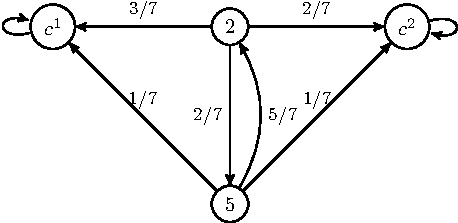
\includegraphics[keepaspectratio]{06-processi_discreti_files/figure-pdf/unnamed-chunk-13-1.pdf}}
\end{center}

In questo caso, le matrici \(\bar{Q}_{TT} = Q_{TT}\) e \(\bar{Q}_{TC}\)
sono rispettivamente
\[ Q_{TT} = \bra{ \begin{array}{cc} 0 & 2/7 \\ 5/7 & 0 \end{array}},\]
mentre
\[ \bar{Q}_{TC} = \bra{ \begin{array}{cc} 3/7 & 2/7 \\ 1/7 & 1/7 \end{array}}. \]
Osserviamo che \(\det(Id - Q_{TT})  = 1-10/49 = 39/49>0\), da cui
\[ (Id - Q_{TT})^{-1} = \frac {49}{39} \bra{ \begin{array}{cc} 1 & 2/7 \\ 5/7 & 1  \end{array}}\]
Si conclude quindi che \(\alpha\) vale
\[ \begin{split} \alpha & = (Id - Q_{TT})^{-1}\bar{Q}_{TC} = \frac {49}{39} \bra{ \begin{array}{cc} 1  & 2/7 \\  5/7 & 1 \end{array}} \bra{ \begin{array}{cc} 3/7 & 2/7 \\ 1/7 & 1/7 \end{array}} \\
& = \frac {1}{39}  \bra{ \begin{array}{cc} 23 & 16 \\ 12 & 17 \end{array}}.\end{split} \]

\subsection{Esercizi}\label{esercizi-36}

Rita e Bruno effettuano il seguente ``gioco'': da un'urna contenente
\(R\) palline rosse e \(B= N-R\) palline blu, si effettuano estrazioni
con rimpiazzo fintanto che non si osservano o due palline rosse estratte
consecutivamente (e in tal caso vince Rita) o due palline blu estratte
consecutivamente (e in tal caso vince Bruno). Si può modellizzare tale
gioco tramite una catena di Markov sull'insieme degli stati
\(E = \cur{RR, RB, BR, BB}\), in cui si tiene conto delle ultime due
estrazioni effettuate. In particolare lo stato \(RR\) rappresenta la
vittoria di Rita, lo stato \(BB\) quella di Bruno. Calcolare tutte le
distribuzioni invarianti. Visualizzare con un grafico la variazione
totale tra la densità marginale al tempo \(t\) e il tempo successivo
\(t+1\), per \(t=0,1,2,\ldots, 10\).

\section{Stima dei parametri}\label{sec-mle-markov}

In questa sezione consideriamo il problema di stimare i \emph{parametri}
di un processo di Markov omogeneo, sulla base di osservazioni di una
traiettoria. Per quanto visto nelle sezioni precedenti, i parametri sono
la matrice delle probabilità di transizione \(Q\) per una catena di
Markov \((X_n)_{n}\) o delle intensità di salto \(L\) per un processo di
Markov a salti \((X_t)_t\), ed eventualmente la densità discreta della
marginale al tempo iniziale.

Per semplificare l'esposizione, consideriamo prima il caso di una catena
di Markov \((X_n)_n\) su un insieme di stati \(E\), in cui sia noto che
\(X_0 = x_0\). Richiamando per chiarezza il robot ideale, in questo caso
la matrice di transizione \(Q\) non è nota al robot, ma esso viene
informato che \(X\) segue un cammino
\(\gamma = (x_0 \to x_1 \to \ldots \to x_n)\), ossia \(X_0 = x_0\),
\(X_1=x_1\), \ldots, \(X_n = x_n\) (brevemente scriviamo
\(X = \gamma\)). L'approccio bayesiano consiste nel considerare la
matrice di transizione \(Q\) come una variabile aleatoria
\(\mathcal{Q}\) a valori nelle matrici quadrate \(\R^{E \times E}\) (più
precisamente, sappiamo che i possibili valori di \(\mathcal{Q}\) sono
matrici stocastiche). Avendo stabilito una densità \emph{a priori} per
\(\mathcal{Q}\), ad esempio uniforme sulle matrici stocastiche, la
densità a posteriori è data dalla formula di Bayes
\[  p( \mathcal{Q} = Q | X = \gamma) \propto p(\mathcal{Q} =Q )  L( \mathcal{Q} =Q ; X = \gamma),\]
dove la verosimiglianza \(L\) è definita al solito come
\[ L( \mathcal{Q} =Q ; X = \gamma) = P(X=\gamma| \mathcal{Q} = Q) = P(X_0 = x_0) Q_\gamma = Q_{\gamma},\]
perché è noto a priori che \(X_0 = x_0\). Il peso del cammino osservato
può essere riscritto raccogliendo i fattori ripetuti, ossia
\[ Q_\gamma = \prod_{k=1}^n Q_{x_{k-1} \to x_{k}} = \prod_{i,j \in E} Q_{i\to j}^{\gamma_{i\to j}},\]
dove \(\gamma_{i\to j}\) indica il numero di transizioni dallo stato
\(i\in E\) a \(j \in E\) che avvengono nel cammino \(\gamma\). In
particolare, vale \[ n = \sum_{i,j \in E} \gamma_{i\to j}.\] Se la
densità a priori per \(\mathcal{Q}\) è uniforme (sull'insieme delle
matrici stocastiche), ossia \(p(\mathcal{Q} = Q) \propto 1\), la densità
a posteriori è
\[ p(\mathcal{Q} = Q| X = \gamma) \propto L(\mathcal{Q} = Q; X=\gamma) = Q_\gamma = \prod_{i,j \in E} Q_{i\to j}^{\gamma_{i\to j}}.\]
Osserviamo che la densità è un prodotto delle marginali, ma dovendo
essere \(\mathcal{Q}\) una matrice stocastica le componenti relative ad
una stessa riga \(i\), ad esempio \(\mathcal{Q}_{i \to j}\),
\(\mathcal{Q}_{i \to k}\) non sono indipendenti (la somma deve essere
\(1\)). Possiamo tuttavia affermare che variabili aleatorie associate
alle righe di \(\mathcal{Q}\) sono tra loro indipendenti.

Per calcolare il punto di massimo, ossia la stima di massima
verosimiglianza \(Q_{\mle}\) dobbiamo tenere conto del vincolo che la
somma delle righe della matrice \(\mathcal{Q}\) valga \(1\). Il metodo
generale per determinare massimi o minimi di funzioni vincolate consiste
nell'introduzione di moltiplicatori di Lagrange, in modo da esprimere
che nei punti critici il gradiente della funzione sia ortogonale al
vincolo. Nel nostro caso, il vincolo però è così semplice che possiamo
evitare l'uso di questa tecnica semplicemente esprimendo la diagonale di
\(\mathcal{Q}\) in funzione delle altre entrate sulla riga:
\[ Q_{i \to i} = 1 - \sum_{j \neq i} Q_{i \to j} \quad \text{per ogni $i \in E$.}\]
Possiamo quindi riscrivere la verosimiglianza nel seguente modo
\[ L( \mathcal{Q} = Q ; X=\gamma) = \prod_{i\in E}(1- \sum_{j \neq i} Q_{i \to j})^{\gamma_{i \to i}} \prod_{j \neq i}Q_{i\to j}^{\gamma_{i \to j}}.\]
Poiché le righe sono tra loro indipendenti, possiamo ragionare
separatamente per ciascuna riga \(i\), ossia determinare il massimo
della funzione
\[(Q_{i\to j})_{j \neq i} \mapsto (1- \sum_{j \neq i} Q_{i \to j})^{\gamma_{i \to i}}  \prod_{j \neq i} Q_{i \to j}^{\gamma_{i \to j}},\]
ovvero, passando al logaritmo,
\[ \gamma_{i\to i} \log (1- \sum_{j \neq i} Q_{i \to j})  +\sum_{j \neq i} \gamma_{i \to j} \log(Q_{i \to j}).\]
Imponendo che la derivata rispetto a ciascuna variabile \(Q_{i\to k}\)
(per \(k \neq j\) si annulli, troviamo l'equazione
\[0 = \frac{d}{d Q_{i\to k}} \gamma_{i\to i} \log (1- \sum_{j \neq i} Q_{i \to j})  +\sum_{j \neq i} \gamma_{i \to j} \log(Q_{i \to j}) = -\frac{\gamma_{i \to i}}{1- \sum_{j \neq i} Q_{i \to j}} + \frac{\gamma_{i \to k}}{Q_{i \to k}}.\]
da cui
\[ Q_{i \to k} = \gamma_{i \to k} \cdot \frac{1- \sum_{j \neq i} Q_{i \to j}}{\gamma_{i \to i}}\]
Il secondo termine nel prodotto sopra non dipende da \(k\), e quindi
sommando questa relazione per \(k \neq i\) troviamo che
\[ \sum_{k \neq i} Q_{i \to k} = \sum_{k \neq i} \gamma_{i \to k } \frac{1- \sum_{j \neq i} Q_{i \to j}}{\gamma_{i \to i}}.\]
Ricordando che \(Q_{i \to i} = 1- \sum_{j \neq i} Q_{i \to j}\) abbiamo
quindi la relazione
\[ 1- Q_{i \to i} = \frac{ \sum_{k \neq i} \gamma_{i \to k } }{ \gamma_{i \to i}} Q_{i \to i},\]
da cui ricaviamo che
\[Q _{i \to i} = \frac{\gamma_{i \to i}}{\sum_{j \in E }\gamma_{i \to j}}.\]
In altre parole, abbiamo trovato che la densità discreta di probabilità
\((Q_{i \to k})_{k \in E}\) è proporzionale al numero di salti osservati
\((\gamma_{i \to k})_{k \in E}\),
\[ Q_{i \to k} \propto \gamma_{i \to k}\] o più esplicitamente
\[ Q_{i \to k} = \frac{\gamma_{i \to k}}{\sum_{j \in E } \gamma_{i \to j}}.\]

\begin{remark}
L'espressione sopra per la densità a posteriori e i calcoli per la stima
di massima verosimiglianza suggerisce altre densità a priori (dette di
\emph{Dirichlet}) della forma
\[ p(\mathcal{Q}= Q) \propto \prod_{i,j \in E} Q_{i\to j}^{\alpha_{ij}},\]
per opportuni parametri \(\alpha_{ij}\ge 0\) (dove a essere precisi
bisognerebbe scrivere \(Q_{i \to i} = 1- \sum_{j \neq i} Q_{i \to j}\)).
Notiamo che i calcoli per la stima di massima verosimiglianza mostrano
anche che la moda della densità sopra è data dalla matrice
\[ Q_{i \to j} = \frac{ \alpha_{ij}}{\sum_{k \in E} \alpha_{ik}}.\] La
formula di Bayes darebbe quindi come densità a posteriori
\[ p(\mathcal{Q}= Q | X = \gamma ) \propto \prod_{i,j \in E} Q_{i\to j}^{\alpha_{ij} +\gamma_{i \to j}},\]
e di conseguenza la stima di massima densità a posteriori
\(\mathcal{Q}_{MAP}\), seguendo gli stessi calcoli della stima di
massima verosimiglianza, è
\[ Q_{i \to j} =\frac{  \alpha_{ij}+\gamma_{i \to j}}{ \sum_{k \in E} \alpha_{ik} + \gamma_{i \to k}}.\]
\end{remark}

\begin{remark}
Abbiamo supposto che il cammino osservato parta al tempo \(0\) da
\(x_0\). Tuttavia se iniziasse da un tempo successivo, allora si pone il
problema di stimare \(X_0\). Si può assumere ad esempio che \(X\) sia
stazionaria, e quindi supporre che \(\pi_0\) sia una distribuzione
invariante. Il problema è che questa dipende da \(Q\) in modo tutt'altro
che banale.
\end{remark}

Nel caso di processi di Markov a salti, l'argomento è analogo ma si basa
sulla formula \textbf{?@eq-likelihood-jump-process}. Per brevità non
consideriamo l'approccio bayesiano ma presentiamo solo la stima di
massima verosimiglianza. Si consideri un cammino
\(\gamma = (x_0\to x_1 \ldots x_n)\) che rimane per un tempo \(t_1\)
nello stato \(x_0\), \(t_2\) nello stato \(x_1\) ecc., e si supponga di
osservare \(X = \gamma\), ossia tutta la traiettoria da \(X_0 = x_0\)
fino a \(X_{t_1+\ldots +t_n} = x_n\). Allora la stima di massima
verosimiglianza per la matrice di intensità di salto
\(\mathcal{L}_{MLE}\) si ottiene massimizzando l'espressione
\[ \prod_{k=1}^n \exp\bra{t_k L_{x_{k-1} \to x_{k-1}}}  L_{x_{k-1} \to x_k} = \prod_{i \in E}  \exp\bra{\gamma_{i \to i} L_{i\to i} } \prod_{ i\neq j \in E} L_{i\to j}^{\gamma_{i \to j}}\]
dove stavolta si è posto \(\gamma_{i \to i}\) il tempo totale trascorso
dal cammino nello stato \(i \in E\). Inoltre, poiché la somma delle
righe di \(L\) è nulla, possiamo porre
\[ \exp\bra{\gamma_{i \to i} L_{i\to i} } =  \exp\bra{- \gamma_{i \to i} \sum_{j \neq i} L_{i\to j} }.\]
Passando ai logaritmi e derivando rispetto a ciascun parametro
\(L_{i \to j}\) si ottiene che \(\mathcal{L}_{MLE}\) è data
dall'espressione, per \(i \neq j\),
\[  L_{i \to j} = \frac{ \gamma_{i \to j}}{\gamma_{i \to i} }.\]

\begin{remark}
Negli esempi sopra si suppone di osservare completamente la catena \(X\)
in un intervallo (discreto o continuo) di tempi. Più in generale ci si
può chiedere cosa accada se mancano le osservazioni delle variabili
\(X_k\) in alcuni tempi, oppure se si osserva solamente una funzione
\(g(X_k)\) della catena invece, di \(X_k\), o più in generale una
funzione \(g(X_k, Z_k)\) dove \(Z\) è un processo indipendente da \(X\).
Un esempio fondamentale è dato dal caso in cui \(X\) è un segnale e
\(Z\) è un ``rumore'' che si vorrebbe rimuovere, o \textbf{filtrare}. In
queste situazioni si parla di modelli di Markov nascosti (in inglese
\emph{Hidden Markov Models}, HMM) che hanno molteplici applicazioni.
Opportune modifiche degli argomenti visti sopra permettono di introdurre
algoritmi specifici per stimare i parametri di un HMM, come pure stimare
\(X_k\) dalle osservazioni \(g(X_k, Z_k)\) o anche effettuare
previsioni.
\end{remark}

\subsection{Esercizi}\label{esercizi-37}

\section{Cenni alla teoria delle code}\label{sec-code}

I processi a stati discreti che abbiamo introdotto sopra hanno
applicazioni in tantissimi ambiti. In questa sezione mostriamo come
semplici modelli possano essere utilizzati per studiare la \emph{teoria
delle code}, ossia delle linee d'attesa che si possono formare in
situazioni realistiche, ad esempio quando più persone vogliono accedere
ad un servizio (entrare in un negozio, o pagare alla cassa), oppure dei
veicoli si presentano ad un casello autostradale, o ancora delle istanze
di calcolo che devono essere eseguite da una o più processori in un
computer. Lo studio delle code permette di individuare strategie per
migliorare l'esperienza di chi è in attesa (ridurre i tempi) rendendone
più efficiente il servizio (e quindi eventualmente ridurre i costi). La
teoria delle code è un campo molto esteso e noi ne presentiamo solamente
i modelli più semplici come esempi interessanti di processi di Markov a
salti.

Usiamo il termine \textbf{clienti} (in inglese si usa anche il termine
\emph{jobs}) per indicare genericamente le persone, le auto, i processi
ecc. che nello specifico esempio di coda devono essere serviti da uno o
più \textbf{serventi} (in inglese \emph{servers}).

Gli aspetti fondamentali che si vogliono modellizzare di una coda sono
l'ingresso di uno o più clienti, l'attesa (eventualmente nulla) che un
servente prenda in carico il compito richiesto, e infine l'uscita dalla
coda quando il compito è svolto. Una volta introdotto un modello di
coda, è di interesse calcolare quantità come il tempo medio di attesa,
il numero medio di clienti in coda, ma anche ovviamente stimare i
parametri di un modello sulla base di quantità osservate in una coda
reale.

Per classificare i vari modelli di code studiati in letteratura, Kendall
propose una notazione abbreviata\footnote{https://en.wikipedia.org/wiki/Kendall\%27s\_notation}:
si usano due lettere e un numero (\(A/S/c\)), in cui la prima lettera
(\(A\)) indica un ``processo'' di arrivo dei clienti, la seconda (\(S\))
la legge del tempo di servizio per ciascun cliente, e il numero \(c\) il
numero dei serventi.

In questa sezione consideriamo solamente i modelli \(M/M/c\), in cui gli
arrivi e i servizi sono Markoviani a tempi continui, più precisamente
con tempi esponenziali di due parametri (\(\lambda\) per il tasso di
arrivo dei clienti e \(\pi\) per il servizio), e sono quindi formalmente
definiti come processi di Markov a salti nell'insieme degli stati
\(E = \mathbb{N}\). Lo stato \(n \in E\) rappresenta infatti la
situazione in cui vi siano \(n\) clienti in servizio oppure in attesa di
essere serviti. Una volta che un cliente è servito, esso ``scompare''
dalla coda, che quindi passa dallo stato \(n\) allo stato \(n-1\).
L'arrivo di un cliente è invece rappresentato con una transizione dallo
stato \(n\) allo stato \(n+1\) (non supporremo mai che due o più clienti
arrivino oppure lascino la coda allo stesso istante). A seconda del
numero di serventi \(c\) definiamo una matrice delle intensità di salto
diversa.

\subsection{Processo di Poisson}\label{processo-di-poisson}

Il modello più semplice rappresenta la situazione in cui non vi siano
serventi (o meglio si è interessati solo al processo di arrivo dei
clienti): potrebbe essere classificato come \(M/M/0\), anche se più
comunemente è detto \emph{processo di Poisson} di intensità
\(\lambda>0\) (il tasso di ingresso dei clienti in coda). Le uniche
transizioni avvengono da uno stato \(n\) a uno stato \(n+1\), e si pone,
per ogni \(n \in \mathbb{N}\),
\[ L_{n \to n+1} = \lambda, \quad L_{n \to n} = - \lambda\] e
\(L_{n \to k} = 0\) se \(k \neq n\), \(k \neq n+1\).

\begin{figure}[H]

{\centering \pandocbounded{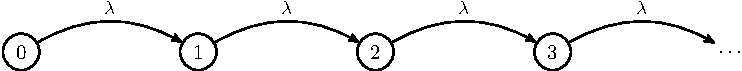
\includegraphics[keepaspectratio]{06-processi_discreti_files/figure-pdf/unnamed-chunk-14-1.pdf}}

}

\caption{grafo associato al processo di Poisson}

\end{figure}%

Ogni stato è quindi transitorio, e non esiste una distribuzione
invariante. Infatti, se \(\pi\) fosse invariante, allora
\[ 0 = (\pi L)_0 = \pi_0 L_{0 \to 0} = - \pi_0 \lambda \quad \text{e quindi} \quad \pi_0 = 0,\]
mentre
\[ 0 = (\pi L)_1 = \pi_0 L_{0 \to 1} + \pi_1 L_{1\to 1} = - \pi_1 \lambda \quad \text{e quindi} \quad \pi_1 = 0,\]
e similmente si ottiene, per ogni \(n \ge 1\), \(\pi_n = 0\). Non è
possibile quindi che \(\pi\) sia una densita discreta di probabilità
(non può essere \(\sum_{n} \pi_n = 1\)).

C'è un legame preciso tra il processo di Poisson e la densità discreta
di Poisson definita nell'Esempio \textbf{?@exm-poisson-density}.
Infatti, se definiamo, per ogni \(t \ge 0\),
\[ \pi^t_n \propto \frac{ (t \lambda)^n}{n!} =\frac{ (t \lambda)^n}{n!} \exp\bra{-t\lambda}.\]
la densità Poisson di parametro \(t \lambda\), allora \(\pi^t\) è la
densità della marginale \(X_t\) di un processo di Poisson tale che
\(X_0 = 0\) (la densità \(\pi^0\) vale infatti \(1\) nel valore \(0\)).
Basta verificare che valga la \emph{master equation}, per ogni
\(n \in \mathbb{N}\), \(t \ge 0\), \[ 
\frac{d}{dt} \pi^t_n = (\pi^t L)_n = \begin{cases} - \lambda \pi^t_0  &\text{se $n=0$,} \\
\lambda( \pi^t_{n-1}  - \pi^t_n ) & \text{se $n \ge 1$.}\end{cases}
\] Calcoliamo quindi
\[ \frac {d}{dt} \exp\bra{-t\lambda}\frac{ (t \lambda)^n}{n!} = \begin{cases} - \lambda  \exp\bra{- t \lambda} & \text{se $n=0$,}\\
  \frac{ n t^{n-1} \lambda^n}{n!} \exp\bra{- t \lambda} - \lambda  \frac{(t\lambda)^n}{n!} \exp\bra{- t \lambda} & \text{ se $n \ge 1$.}
  \end{cases}
\] Per concludere nel caso \(n \ge 1\) basta notare che
\[\frac{ n t^{n-1} \lambda^n}{n!} \exp\bra{- t \lambda}  = \lambda \frac{ (t\lambda)^{n-1}}{(n-1)!}  \exp\bra{- t \lambda} = \lambda \pi^t_{n-1}.\]
Consideriamo infine il problema di stimare il parametro \(\lambda\) a
partire dall'osservazione di un cammino
\(\gamma = (x_0 \to x_1 \to \ldots \to x_{n})\) con tempi di permanenza
\(t_1\) (nello stato \(x_0\)), \(t_2\) (in \(x_1\)), \ldots.,
\(t_{n+1}\). Osserviamo che, poiché i salti avvengono solo tra uno stato
\(n\) e il successivo \(n+1\), deve essere \(x_1 = x_0+1\),
\(x_2=x_0+2\), ecc., quindi la formula per la verosimiglianza in questo
caso diventa
\[ L( \Lambda = \lambda; X = \gamma) = \prod_{k=1}^n \exp\bra{- \lambda t_k} \lambda = \lambda^n  \exp\bra{- \lambda T}.
\] dove abbiamo supposto per semplicità che fosse noto a priori che
\(X_0 = x_0\) e abbiamo indicato con \(T = \sum_{k=1}^n t_k\). La stima
di massima verosimiglianza \(\lambda_{MLE}\) si trova passando al
logaritmo e imponendo che la derivata si annulli. Si trova
\[ \frac{n}{\lambda_{MLE}} - T = 0 \quad \text{quindi} \quad \lambda_{MLE} = \frac{n}{T}.\]

In un intervallo di tempo \(T = 5\) minuti si osservano entrare
\(n = 10\) persone in un supermercato. Si può introdurre quindi un
processo di Poisson con intensità \(\lambda = 2\) (persone/minuto) per
modellizzare gli ingressi.

Per un approccio bayesiano, in cui i calcoli siano particolarmente
semplici si può introdurre una densità a priori per la variabile
\(\Lambda\) del tipo \emph{Gamma}, ossia
\[ p(\Lambda = \lambda) \propto \lambda^{\alpha-1 } \exp\bra{ - \beta \lambda },\]
dove \(\alpha\), \(\beta>0\) sono parametri (si scrive anche
\(\Gamma(\alpha, \beta)\)). Il valor medio di \(\Lambda\) (a priori) si
può calcolare ed è dato da \(\alpha/\beta\), mentre la moda è
\((\alpha-1)/\beta\) (per \(\alpha\ge 1\)). Nel caso \(\alpha=1\) essa
coincide con una densità esponenziale di parametro \(\beta\). Questa
densità rappresenta in modo preciso una possibile informazione nota sul
parametro \(\lambda\), ad esempio informalmente che
\(\lambda \approx \alpha/\beta\).

La densità a posteriori diventa quindi
\[ p(\Lambda = \lambda| X = \gamma) \propto \lambda^{n+\alpha-1 } \exp\bra{ -(\beta+T) \lambda },\]
ossia una densità \(\Gamma(n+\alpha, \beta+T)\). La moda della densità a
posteriori è quindi (se \(n +\alpha \ge 1\))
\[ \lambda_{MAP} = \frac{ n+\alpha}{T +\beta}.\]

\subsection{\texorpdfstring{Code \(M/M/1\)}{Code M/M/1}}\label{code-mm1}

Consideriamo ora la situazione in cui vi sia un solo servente
(\(M/M/1\)), e che il tempo di servizio per ciascun cliente sia una
variabile esponenziale di parametro \(\mu\) (ogni cliente sia
indipendente dagli altri). Per modellizzare la coda con un processo di
Markov a salti, conviene considerare prima il caso in cui non vi siano
arrivi. In tal caso si osserveranno solamente salti da uno stato \(n\)
verso \(n-1\) (se \(n \ge 1\)) con dei tempi di permanenza esponenziali
di parametro \(\mu\). Pertanto, si avrà (se \(n\ge 1\))
\[L_{n \to n-1} = \mu.\] Nel caso in cui vi siano arrivi con un processo
di Poisson di intensità \(\lambda\), poniamo, per \(n \ge 0\),
\[ L_{n \to n+1} = \lambda,\] e di conseguenza
\[ L_{ n \to n} = \begin{cases} -\lambda & \text{se $n = 0$}\\
-(\lambda + \mu) & \text{se $n \ge 1$,}\end{cases}\] avendo posto
\(L_{ n \to k} = 0\) se \(k \notin \cur{n-1, n, n+1}\).

\begin{figure}[H]

{\centering \pandocbounded{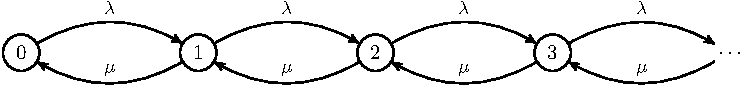
\includegraphics[keepaspectratio]{06-processi_discreti_files/figure-pdf/unnamed-chunk-15-1.pdf}}

}

\caption{grafo associato ad una coda \(M/M/1\)}

\end{figure}%

Ogni stato è ricorrente, ma essendo infiniti stati non è ovvio che
esista una distribuzione invariante. Vi è infatti una competizione tra
il tasso di arrivo \(\lambda\) e di uscita \(\mu\). Analogamente a
quanto fatto nel caso di Poisson, si può risolvere l'equazione
\(\pi L = 0\) e ottenere per \(n \ge 0\),
\[\pi_n \propto \bra{ \frac{\lambda}{\mu}}^n.\] È un semplice esercizio
verificare che \(\pi\) soddisfa l'equazione, ossia
\[ 0 = (\pi L)_n = \pi_{n-1} L_{n-1 \to n} + \pi_n L_{n\to n} +\pi_{n+1}L_{n+1\to n} = \lambda \pi_{n-1} -(\lambda+\mu) \pi_n + \mu \pi_{n+1}\]
(per \(n \ge 1\), mentre per \(n=0\) bisogna porre
\(L_{-1 \to 0} = 0\)).

Dovendo garantire che tale \(\pi\) sia una densità di probabilità,
bisogna che \[\sum_{n} \bra{ \frac\lambda \mu}^n < \infty,\] ma tale
serie (geometrica) converge se e solo se \(\lambda<\mu\). In altri
termini, esiste un equilibrio per la coda se e solo se il tasso di
arrivo è strettamente minore di quelo di uscita, altrimenti il numero di
persone in coda cresce (più lentamente del processo di Poisson, ma
comunque in modo inarrestabile).

La distribuzione invariante se \(\lambda<\mu\) è quindi una densità
geometrica di parametro \(1-\lambda/\mu\). In particolare, il valor
medio del numero di clienti nella coda (in attesa o in servizio) \(N\)
in regime stazionario (ossia se la marginale del processo a salti è
\(\pi\)) vale
\[ \E{N} = \sum_{n} n \pi_n = \frac{\lambda}{\mu -\lambda},\] una
quantità che diverge al tendere di \(\lambda\) verso \(\mu\).

\begin{Shaded}
\begin{Highlighting}[]
\NormalTok{deltal }\OtherTok{=} \FloatTok{0.001}
\NormalTok{l }\OtherTok{=} \FunctionTok{seq}\NormalTok{(}\FloatTok{0.5}\NormalTok{,}\FloatTok{0.99}\NormalTok{, }\AttributeTok{by=}\NormalTok{deltal)}
\NormalTok{mu}\OtherTok{=}\DecValTok{1}

\FunctionTok{plot}\NormalTok{(l, l}\SpecialCharTok{/}\NormalTok{(}\DecValTok{1}\SpecialCharTok{{-}}\NormalTok{l), }\AttributeTok{type=}\StringTok{\textquotesingle{}l\textquotesingle{}}\NormalTok{, }\AttributeTok{col=}\NormalTok{miei\_colori[}\DecValTok{2}\NormalTok{], }\AttributeTok{lwd=}\DecValTok{3}\NormalTok{, }\AttributeTok{xlab =} \StringTok{"tasso di ingresso"}\NormalTok{, }\AttributeTok{ylab=} \StringTok{"numero medio di clienti"}\NormalTok{)}
\FunctionTok{abline}\NormalTok{(}\AttributeTok{h=}\DecValTok{50}\NormalTok{, }\AttributeTok{col=}\NormalTok{miei\_colori[}\DecValTok{1}\NormalTok{], }\AttributeTok{lwd=}\DecValTok{3}\NormalTok{)}
\end{Highlighting}
\end{Shaded}

\begin{figure}[H]

{\centering \pandocbounded{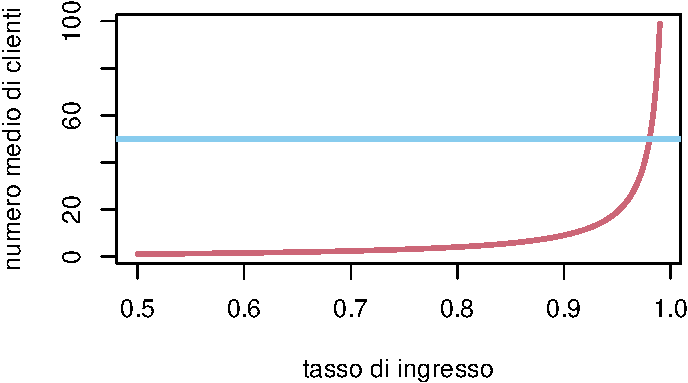
\includegraphics[keepaspectratio]{06-processi_discreti_files/figure-pdf/unnamed-chunk-16-1.pdf}}

}

\caption{grafico di \(\E{N}\) per \(\mu=1\) in funzione di \(\lambda\)
(in rosso) e una soglia massima di possibili persone in coda (in
azzurro)}

\end{figure}%

Tale divergenza è problematica se \(\lambda\) si trova molto vicino a
\(\mu\) e per qualche motivo il tasso di ingresso aumenta, anche di
poco, portando a superare il limite massimo possibile di clienti in coda
(che nella realtà esiste sempre).

Prima della pandemia gli ospedali operavano in modo da usare tutti o
quasi i posti letto disponibili -- usando quindi efficientemente tutte
le risorse di personale e strutture. Rappresentando un ospedale come una
coda, erano quindi molto vicini al limite massimo di possibili
``clienti'' (i pazienti) in coda. L'arrivo del nuovo coronavirus ha
avuto l'effetto di aumentare il tasso di ingresso, causando un aumento
notevole di \(N\) con conseguenze potenzialmente catastrofiche.

Veniamo ora alla stima dei parametri \((\lambda, \mu)\) sulla base
dell'osservazione di un cammino
\(\gamma = (n_0 \to n_1 \to \ldots \to n_\ell)\) con i soliti tempi di
permanenza \(t_1\), \(t_2\), \ldots, \(t_\ell\) e poniamo pure
\(T = \sum_{k=1}^\ell t_i\). Supponiamo inoltre che il cammino osservato
non passi mai per lo stato \(0\) (quindi c'è sempre almeno un cliente in
coda). Usando l'espressione \textbf{?@eq-likelihood-jump-process}, si
ottiene la verosimiglianza
\[ L( \lambda, \mu; X=\gamma) =  \exp\bra{-(\lambda+\mu)T} \lambda^{\gamma_+} \mu^{\gamma_-},\]
dove \(\gamma_+\) indica il numero di arrivi osservati in \(\gamma\)
(ossia transizioni da uno stato \(n\) a \(n+1\)), mentre \(\gamma_-\) il
numero di uscite. La stima di massima verosimiglianza è quindi
\[ \lambda_{MLE} = \frac{\gamma_+}{T}, \quad  \mu_{MLE} = \frac{\gamma_-}{T}.\]
Se invece il cammino trascorre un tempo \(T_0\) nello stato \(0\),
l'espressione per la verosimiglianza cambia (al posto di
\(-(\lambda+\mu)T\) si trova \(-\lambda T -\mu (T-T_0)\) e di
conseguenza \(\lambda_{MLE}\) non cambia, ma
\[ \mu_{MLE} = \frac{\gamma_-}{T-T_0}.\] L'interpetazione è che il tempo
trascorso con la coda vuota non può essere utile alla stima del tasso di
uscita dei clienti dalla coda, e quindi va sottratto.

In un intervallo di \(10\) minuti si osservano \(5\) persone arrivare
alla cassa di un supermercato e \(3\) persone uscirne. Supponendo che la
cassa non sia mai senza lavoro si stimano i parametri \(\lambda = 1/2\)
persone al minuto, \(\mu = 3/10\) persone al minuto. Se invece la cassa
è rimasta priva di persone in coda per \(4\) minuti, si stima
\(\mu = 3/6 =1/2\) persone al minuto.

Tralasciamo l'approccio bayesiano, che è simile al caso del Poisson
(supponendo ad esempio \(\lambda\), \(\mu\) indipendenti a priori).

\subsection{\texorpdfstring{Code
\(M/M/\infty\)}{Code M/M/\textbackslash infty}}\label{code-mminfty}

Consideriamo infine la situazione opposta, in cui vi sono un numero
arbitrariamente grande, idealmente infinito, di serventi
(\(M/M/\infty\)). Supponiamo ancora che il tempo di servizio per ciascun
cliente sia una variabile esponenziale di parametro \(\mu\) (e ogni
cliente sia indipendente dagli altri). Per capire quali intensità di
salto definire, conviene considerare ancora il caso in cui non vi siano
arrivi. In tal caso si osserveranno solamente salti da uno stato \(n\)
verso \(n-1\) (se \(n \ge 1\)) con dei tempi di permanenza dati dal
minimo di \(n\) variabili aleatorie \(T_1\), \(T_2\), \ldots, \(T_n\)
esponenziali indipendenti tra loro (infatti, la transizione avviene
appena il cliente che impega meno tempo tra gli \(n\) in servizo lascia
la coda). Possiamo allora affermare che tale tempo è una variabile
esponenziale \(T\), di parametro \(n\mu\): infatti si calcola la
funzione di sopravvivenza (per \(t\ge 0\))
\begin{equation*}\begin{split} \SUR_T(t) & = P( \min \cur{T_1, T_2, \ldots, T_k} > t )\\
& = P( T_1>t, T_2>t, \ldots, T_n >t) \\
& = P(T_1>t) P(T_2>t) \cdot \ldots\cdot  P(T_n>t) \\
& = e^{-\mu t} \cdot e^{-\mu t} \cdot \ldots \cdot e^{-\mu t}\\
& = e^{-n\mu t},
\end{split}
\end{equation*} e derivando si ottiene la densità esponenziale.

Pertanto, si avrà (se \(n\ge 1\)) \[L_{n \to n-1} = n \mu\] Nel caso in
cui vi siano arrivi con un processo di Poisson di intensità \(\lambda\),
poniamo, per \(n \ge 0\), \[ L_{n \to\ n+1} = \lambda,\] e di
conseguenza
\[ L_{ n \to n} = \begin{cases} -\lambda & \text{se $n = 0$}\\
-(\lambda + n\mu) & \text{se $n \ge 1$,}\end{cases}\] avendo posto
\(L_{ n \to k} = 0\) se \(k \notin \cur{n-1, n, n+1}\).

\begin{figure}[H]

{\centering \pandocbounded{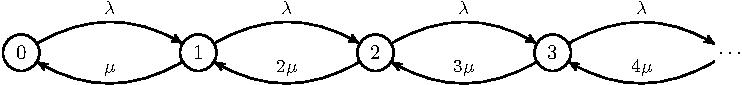
\includegraphics[keepaspectratio]{06-processi_discreti_files/figure-pdf/unnamed-chunk-17-1.pdf}}

}

\caption{grafo associato ad una coda \(M/M/\infty\)}

\end{figure}%

Come nel caso \(M/M/1\), ogni stato è ricorrente, ma essendo infiniti
stati non è ovvio che esista una distribuzione invariante. Vi è ancora
una competizione tra il tasso di arrivo \(\lambda\) e di uscita \(\mu\),
ma decisamente ``smorzata'' dal fatto che per \(n\) abbastanza grande si
avrà comunque \(\lambda <n\mu\). Questo suggerisce che una distribuzione
invariante esista sempre. Infatti, si può risolvere l'equazione
\(\pi L = 0\) e ottenere per \(n \ge 0\),
\[\pi_n \propto \frac{1}{n!} \bra{ \frac{\lambda}{\mu}}^n,\] ossia una
densità Poisson di parametro \(\lambda/\mu\). Lasciamo per esercizio di
verificare che \(\pi\) soddisfa l'equazione \(\pi L = 0\). Il valor
medio del numero di clienti nella coda è quindi \(\E{N} = \lambda/\mu\)
che cresce linearmente al crescere di \(\lambda\) (non presenta
asintoti).

Infine, la stima dei parametri \((\lambda, \mu)\) sulla base
dell'osservazione di un cammino
\(\gamma = (n_0 \to n_1 \to \ldots \to n_{\ell-1})\) con i tempi di
permanenza \(t_1\), \(t_2\), \ldots, \(t_\ell\) si può effettuare
tramite il metodo di massima verosimiglianza, usando l'espressione
\textbf{?@eq-likelihood-jump-process}:
\[ L( \lambda, \mu; X=\gamma) \propto \exp\bra{-\lambda T - \mu T_\gamma )} \lambda^{\gamma_+} \mu^{\gamma_-},\]
dove \(T = \sum_{k=1}^\ell t_i\), \(\gamma_+\) e \(\gamma_-\) sono come
nel caso \(M/M/1\) e infine \[ T_\gamma = \sum_{k=1}^\ell t_i n_i,\] (il
tempo totale trascorso da tutti i clienti osservati nella coda). La
stima di massima verosimiglianza è quindi
\[ \lambda_{MLE} = \frac {\gamma_-}{T}, \quad \mu_{MLE} = \frac{\gamma_-}{T_\gamma}.\]

Un ipermercato dispone di un numero molto grande di casse, e al mattino
è poco frequentato cosicché ogni cliente trova sempre una cassa libera.
Si osserva che per \(4\) minuti consecutivi tutte le casse erano libere,
per \(3\) minuti \(1\) sola cassa era occupata, poi si è liberata per
\(1\) minuto tutte le casse erano di nuovo libere, e infine per \(2\)
minuti in un intervallo di \(10\) minuti minuti tutte le casse erano
libere, per \(3\) minuti una sola cassa era occupata, e per i rimanenti
\(3\) minuti \(5\) casse erano occupate.

\begin{remark}
Il caso generale \(M/M/c\) con \(2 \le c < \infty\) è intermedio tra i
due estremi che abbiamo considerato. In particolare una distribuzione
invariante esiste se e solo se \(\lambda < c\mu\).
\end{remark}

\subsection{Esercizi}\label{esercizi-38}

\section{Problemi}\label{problemi-4}

\bookmarksetup{startatroot}

\chapter{Processi a stati continui}\label{processi-a-stati-continui}

In questo capitolo affrontiamo lo studio dei processi stocastici a stati
continui (e tempi discreti) concentrandoci in particolare nel caso in
cui l'insieme degli stati siano i numeri reali (l'estensione di processi
a valori vettoriali sarà solo accennata).

\begin{itemize}
\item
  Nella Sezione Sezione~\ref{sec-stazionari-continui} introduciamo i
  concetti fondamentali di funzione di media e di autocovarianza (o di
  autocorrelazione) di un processo a valori reali. Vedremo anche una
  nozione più debole di stazionarietà, che tuttavia per l'esempio
  fondamentale dei processi gaussiani coincide con la stazionarietà
  usuale.
\item
  Nella Sezione Sezione~\ref{sec-esempi-wn-rw-se} studiamo tre esempi di
  processi (gaussiani), il rumore bianco, la passeggiata aleatoria e
  l'equazione lineare con smorzamento.
\item
  Le Sezioni Sezione~\ref{sec-arima-def} e Sezione~\ref{sec-arima-prop}
  sono dedicate allo studio modelli di processi a stati continui, detti
  ARIMA, che generalizzano gli esempi visti sopra. Tale classe di
  modelli è molto versatile ed utile nelle applicazioni statistiche
  (detto anche lo studio delle serie storiche).
\item
  Infine, nella Sezione Sezione~\ref{sec-wiener-kinchin}, riprendiamo lo
  studio generale dei processi, affrontando il problema di stimare, a
  partire dalle osservazioni, la funzione di autocovarianza di un
  processo stazionario.
\end{itemize}

\section{Funzione di autocovarianza e
stazionarietà}\label{sec-stazionari-continui}

Dato un processo stocastico \((X_t)_{t \in \mathcal{T}}\) avente come
insieme degli stati \(E = \R\), si può considerare il suo valor medio al
variare del tempo, definendo così la \textbf{funzione di media} del
processo, \[ t \in \mathcal{T} \mapsto \E{X_t},\] e similmente per la
covarianza tra due tempi qualsisasi,
\[ (s,t ) \in \mathcal{T}^2 \mapsto \Cov{X_s, X_t} = K_{X_s X_t}, \]
definendo così la \textbf{funzione di autocovarianza} del processo
\(X\). Una notazione piuttosto comune per tale funzione è
\[ C(s,t) = \Cov{X_s, X_t},\] qualora sia inteso il processo \(X\)
considerato. In alternativa si può indicarla con \(K_{XX}(s,t)\).
Notiamo che \[ C(s,s) = \Cov{X_s, X_s} = \Var{X_s}\] è la varianza.

\begin{remark}
A volte si considera anche la funzione \[ R(s,t) = \E{ X_s X_t},\] che è
legata alle funzioni di autocovarianza e di media tramite la formula
alternativa per il calcolo della covarianza:
\[ R(s,t) = C(s,t) + \E{X_s} \E{X_t}\] Una terza funzione collegata è la
\textbf{funzione di autocorrelazione} (in inglese \emph{autocorrelation
function}, abbreviata spesso con ACF) data da
\[ (s,t) \in \mathcal{T}^2 \mapsto \operatorname{ACF}(s,t) = \rho_{X_s X_t} = \frac{ \Cov{X_s, X_t}}{ \sqrt{ \Var{X_s} \Var{X_t}} }, \]
che ha il vantaggio di essere sempre a valori in \([-1,1]\), essendo un
coefficiente di correlazione. Ricordiamo che valori vicini ad \(1\)
indicano una forte dipendenza lineare tra le variabili, informalmente
\(\operatorname{ACF}(s,t)\approx 1\) indica che che
\(X_s \approx a X_t +b\) per opportune costanti \(a\), \(b\) reali.
\end{remark}

\begin{remark}
Nel caso di \(X\) a valori vettoriali, ossia se \(E = \R^d\), la
funzione di media è a valori in \(\R^d\), mentre l'autocovarianza
\(\Cov{X_s, X_t}\) si estende alla \textbf{funzione di covarianza
incrociata} (o cross-covarianza, \emph{cross-covariance} in inglese),
per ogni coppia di componenti \(i\), \(j \in \cur{1, \ldots, d}\),
definita come \[K_{X_i X_j}(s,t) = \Cov{X_{i,s}, X_{j,t}},\] ossia la
covarianza tra la componente \(i\) del processo al tempo \(s\) e la
componente \(j\) al tempo \(t\). Ci limitiamo tuttavia in questo
capitolo allo studio di processi a valori reali.
\end{remark}

Se il processo è stazionario, le funzioni di media e covarianza
dipendono da ``un parametro'' in meno, ossia la media è costante, mentre
la covarianza dipende solo dalla differenza dei tempi. Vale infatti il
seguente risultato.

Se \(\mathcal{T} = \cur{0,1,2,\ldots, n}\) oppure
\(\mathcal{T} =\mathbb{N}\) e il processo \((X_t)_{t \in \mathcal{T}}\)
è stazionario, allora il valor medio è costante nel tempo,
\[ \E{X_t} = \E{X_0} \quad \text{per ogni $t\in \mathcal{T}$,}\] mente
l'autocovarianza dipende solamente dalla differenza (assoluta) dei due
istanti,
\[ C(s,t) = C(0, |t-s|), \quad \text{per ogni $s$, $t \in \mathcal{T}$.}\]
In particolare, la varianza \(C(s,s) = C(0,0)\) è costante.

\begin{proof}
Il valor medio di \(X_t\) dipende soltanto dalla legge marginale del
processo al tempo \(t\) (ad esempio dalla densità discreta o continua) e
quindi per stazionarietà \(\E{X_t} = \E{X_0}\). Per l'autocovarianza,
supponiamo senza perdita di generalità che \(t \ge s\) e notiamo che
\[ \Cov{ X_s, X_t } = \E { (X_s - \E{X_0})(X_t -\E{X_0})} = \E{ g(X_s,X_t)},\]
avendo usato il fatto che \(\E{X_s}= \E{X_t} = \E{X_0}\) e la funzione
\[g (x, y) = (x- \E{X_0}) (y - \E{X_0}).\] Ricordando che la
stazionarietà implica che la legge congiunta di \((X_s, X_t)\) coincide
con quella di \((X_0, X_{t-s})\), segue che
\[ \Cov{X_s, X_t } = \E{ g(X_s, X_t)}  = \E{ g(X_0, X_{t-s})}= C(0, t-s).\]
\end{proof}

Il risultato sopra motiva il seguente indebolimento del concetto di
stazionarietà, in cui ci si limita a considerazioni sulla media e
l'autocovarianza.

Supponiamo che \(\mathcal{T}=\cur{0,1, \ldots, n}\) oppure
\(\mathcal{T} = \mathbb{N}\). Un processo \((X_t)_{t \in \mathcal{T}}\)
è \textbf{stazionario in senso lato}, se
\[ \E{X_t} = \E{X_0} \quad \text{per ogni $t$,}\] e
\[ C(s,t) = C(0, |t-s|), \quad \text{per ogni $s$, $t \in \mathcal{T}$.}\]

In generale questa nozione è più debole (ad esempio le informazioni sui
momenti primi e secondi non implicano nulla sui momenti di ordine terzo,
quarto ecc.). Per distinguere tra questa nozione e la vera e propria
stazionarietà, a volte quest'ultima è detta stazionarietà in \emph{senso
stretto}.

Tuttavia, se il processo \(X\) è \textbf{gaussiano}, ossia ogni
variabile congiunta \[(X_{t_1}, X_{t_2}, \ldots, X_{t_d}),\] per
qualsiasi scelta \(t_1, t_2, \ldots, t_d \in \mathcal{T}\) è un vettore
aleatorio gaussiano, allora dalla stazionarietà in senso lato segue la
stazionarietà in senso stretto (la vera e propria stazionarietà). Questo
perché, per ogni \(s \in \mathbb{T}\) tale che
\(t_d+s \in \mathcal{T}\), i parametri di media e di covarianza delle
variabili gaussiane vettoriali
\[(X_{t_1}, X_{t_2}, \ldots, X_{t_d}) \quad \text{e} \quad (X_{t_1+s}, X_{t_2+s}, \ldots, X_{t_d+s})\]
coincidono: il vettore delle medie è uguale per entrambi (vale per
ciascuna variabile marginale \(\E{X_0}\)), mentre, per la matrice delle
covarianze troviamo che
\[ \Cov{X_{t_i}, X_{t_j} } = C(t_i, t_j) = C(0, |t_i-t_j|) = C(t_i+s, t_j+s) = \Cov{X_{t_i+s}, X_{t_j+s} }.\]

\section{Esempi}\label{sec-esempi-wn-rw-se}

In questa sezione descriviamo alcuni modelli fondamentali di processi a
stati continui, calcolandone esplicitamente la funzione di
autocovarianza e discutendone la gaussianità e stazionarietà. Nella
sezione successiva inquadreremo questi processi come casi particolari di
una famiglia di processi, detta ARIMA.

\subsection{Rumore bianco gaussiano}\label{rumore-bianco-gaussiano}

Il più semplice processo a stati continui che consideriamo consiste di
variabili aleatorie \((W_t)_{t \in \mathcal{T} }\), tutte con la
medesima legge e indipendenti. Tale processo assume vari nomi a seconda
dell'ambito di studio e in particolare a seconda della legge comune
delle marginali. Ad esempio, nel caso di variabili Bernoulli
indipendenti, tutte aventi lo stesso parametro \(p \in [0,1]\), ossia
\(P(W_t = 1) = p\) per ogni \(t \in \mathcal{T}\), il processo è detto
processo di Bernoulli.

In questo capitolo ci concentriamo invece sui processi a stati continui,
e il caso che consideriamo è quando tutte le marginali \(W_t\) siano
variabili reali, tutte con medesima densità continua gaussiana, di media
nulla e varianza \(\sigma^2\): la densità della marginale è quindi
\[ p(W_t = w)  = \exp\bra{ - \frac {w^2} {2 \sigma^2} } \frac{1}{\sqrt{ 2 \pi \sigma^2}}.\]
Un tale processo \((W_t)_{t \in \mathcal{T}}\) è detto \textbf{rumore
bianco gaussiano} (in inglese, \emph{Gaussian white noise}, che
giustifica la notazione \(W\)) di \textbf{intensità} \(\sigma^2\),
sull'insieme dei tempi \(\mathcal{T}\).

\begin{remark}
Il termine rumore è motivato dall'utilizzo in modelli di teoria
dell'informazione. Supponendo che un messaggio
\((M_t)_{t \in \mathcal{T}}\), ad esempio una sequenza di bit, venga
trasmesso tramite un mezzo di comunicazione reale (ad esempio tramite
onde elettromagnetiche), per modellizzare l'effetto di molteplici
fenomeni naturali che portano ad una possibile ``distorsione'' nella
ricezione del messaggio, si suppone che il ricevitore osservi il
processo \[  (M_t + W_t)_{t \in \mathcal{T}},\] dove
\((W_t)_{t \in \mathcal{T}}\) è un rumore bianco gaussiano di una certa
intensità \(\sigma^2\) (è un parametro del modello che si può stimare).
Il fatto che il rumore sia sommato spiega perché a volte il rumore
bianco gaussiano è anche accompagnato dall'aggettivo \emph{additivo}.
Notiamo di passaggio che in questi modelli anche il messaggio è trattato
come una variabile aleatoria (per questo usiamo una lettera maiuscola).
Questo è evidente se lo pensiamo dal punto di vista del ricevente, ma
anche se assumiamo il punto di vista dell'ingegnere che deve
studiare/progettare il mezzo di comunicazione e possibilmente
contrastare l'effetto del rumore.
\end{remark}

Consideriamo un rumore bianco gaussiano \((W_t)_{t \in \mathcal{T}}\) di
intensità \(\sigma^2\). La funzione di media, avendo supposte tutte le
\(W_t\) centrate è identicamente nulla: \[  t \mapsto \E{W_t} = 0.\]
Anche la funzione di autocovarianza è molto semplice, ricordando che
variabili indipendenti non sono correlate, mentre per ipotesi
\(\Var{W_t} = \sigma^2\). Pertanto
\[ C(s,t) = \begin{cases} 0 & \text{ se $s \neq t$,}\\
 \sigma^2  & \text{ se $ s = t$.}\end{cases}\] A volte si usa una
notazione abbreviata introducendo la funzione delta (di Dirac discreta)
centrata in \(0\), definita così:
\[ \delta_0(x) = \begin{cases} 0 & \text{se $x \neq 0$,}\\
 1 & \text{se $x=0$.}\end{cases}
 \] Si trova allora che \[ C(s,t)= \sigma^2 \delta_0( t-s).\] In
particolare, il processo è stazionario in senso lato. Essendo un
processo gaussiano, è anche stazionario in senso stretto.

\begin{remark}
Se il parametro \(\sigma^2\) non è noto, si può stimarlo da \(n\)
osservazioni \(W_{t_i} = w_i\), riconoscendo che il problema è lo stesso
della stima della varianza di un campione gaussiano (di cui la media è
nota). In particolare la stima di massima verosimiglianza in questo caso
è data da \[ \sigma_{\mle}^2 = \frac 1 n \sum_{i=1}^n  w_i^2.\]
\end{remark}

Per comprendere l'aggettivo \emph{bianco} è invece necessario
considerare la trasformata di Fourier del processo. Supponiamo, per
evitare di considerare serie, che l'insieme dei tempi sia finito e
precisamente \(\mathcal{T} = \cur{0, 1, \ldots, n-1}\). Allora la
trasformata di Fourier di \((W_t)_{t=0}^{n-1}\) è data da
\[ \hat{W}(\xi) = \sum_{t=0}^{n-1} W_t e^{-2 \pi i \xi t/n}.\] In
particolare, osserviamo che per ciascuna frequenza
\(\xi \in \cur{0, \ldots, (n-1)}\) la variabile aleatoria
\(\hat{W}(\xi)\) è una combinazione lineare (a coefficienti complessi)
di variabili gaussiane indipendenti. Il fatto che siano complesse
complica un po' la cosa, perché vanno pensate come variabili gaussiane
vettoriali a valori in \(\R^2\), ma si può mostrare che sono comunque
variabili gaussiane. Il valor medio di ciascuna di esse è, usando la
linearità,
\[ \E{ \hat{W}(\xi)} = \sum_{t=0}^{n-1} \E{W_t} e^{-2 \pi i \xi t/n} =  0,\]
mentre il valor medio dell'energia associata a ciascuna frequenza
\(\xi\) è \[
\begin{split}
\E{ | \hat{W}(\xi) |^2 } &  = \E{  \hat{W}(\xi) \overline{ \hat{W} (\xi)} } \\
& = \E{ \sum_{t=0}^{n-1} W_te^{-2 \pi i \xi t/n}  \sum_{s=0}^{n-1} W_s e^{2 \pi i \xi s/n}}\\
&  = \sum_{t=0}^{n-1}\sum_{s=0}^{n-1} e^{-2 \pi i \xi (t-s) /n} \E{ W_t W_s}\\
& = \sum_{t=0}^{n-1}\sum_{s=0}^{n-1} e^{-2 \pi i \xi (t-s) /n} \sigma^2 \delta_0(t-s)\\
& = \sigma^2 \sum_{t=0}^{n-1} 1 = \sigma^2 n.
\end{split}\] Quindi l'energia in media su ciascuna frequenza è
costante. Poiché il termine \(n\) è l'intervallo di tempo (supponendo di
aver osservato a istanti temporali equispaziati con intervalli di
ampiezza \(1\)) la quantità \[  \frac{ \E{ | \hat{W}(\xi)|^2 } }{n}\]
può essere pensata come una \emph{potenza} (energia su tempo) media, ed
è un caso particolare del concetto di \textbf{densità spettrale di
potenza}. Ritorneremo su questa nozione, in generale, nella Sezione
Sezione~\ref{sec-wiener-kinchin}.

\subsection{Passeggiata aleatoria
gaussiana}\label{passeggiata-aleatoria-gaussiana}

Il secondo esempio che trattiamo consiste nella somma cumulativa di un
rumore bianco gaussiano \(W\). Precisamente, posto
\(\mathcal{T} = \cur{0,1, \ldots, n}\) o eventualmente
\(\mathcal{T} = \N\), definiamo
\[ S_0 = 0, \quad S_t = W_1+W_2+ \ldots +W_t = \sum_{s=1}^t W_s,\] dove
\((W_s)_{s}\) è un rumore bianco gaussiano di instensità \(\sigma^2\).
Si può in alternativa usare una definizione \emph{ricorsiva} ponendo
\(S_0 = 0\) e per ogni \(t \in \mathcal{T}\), \(t \ge 1\),
\[  S_t = S_{t-1} + W_t.\] In questo caso il processo si intepreta come
una ``passeggiata'', in cui ad ogni istante \(t \ge 1\), partendo dalla
posizione \(S_{t-1}\), si compie un nuovo ``passo'' \(W_t\) e
spostandosi nella posizione \(S_t = S_{t-1}+W_t\). Il processo
\((S_t)_{t}\) è detto \textbf{passeggiata aleatoria gaussiana}.

\begin{remark}
La passeggiata aleatoria, un po' come il rumore bianco, si può anche
considerare con leggi diverse dalla gaussiana. Un esempio nel discreto è
il caso in cui ciascuna \(W_s\) assuma solo valori \(\cur{-1, 1}\), con
probabilità uniforme, detto passeggiata aleatoria simmetrica semplice.
\end{remark}

Tornando alla passeggiata aleatoria gaussiana, la media di ciascuna
\(S_t\) è nulla, infatti
\[ \E{S_t} = \E{ \sum_{s=1}^t W_s} = \sum_{s=1}^t \E{W_s} = 0.\]
Tuttavia la passeggiata aleatoria gaussiana non è un processo
stazionario (neppure in senso lato). Infatti, se lo fosse, la varianza
\(\Var{S_t} = C(t,t)\) dovrebbe essere costante, ma vale
\[ \begin{split} \Var{S_t} & = \Var{ \sum_{i=1}^ t W_i } = \sum_{i=1}^t \Var{W_i} \\
& = \sum_{i=1}^t \sigma^2  = t \sigma^2.\end{split}\] (ovviamente
supponiamo che \(\sigma^2>0\)). Possiamo anche calcolare la funzione di
autocovarianza, dati \(s\), \(t \in \mathcal{T}\), ad esempio con
\(s \le t\),
\[ \begin{split} C(s,t) &= \Cov{S_s, S_t} = \Cov{ S_s, S_s + W_{s+1}+\ldots + W_{t}}\\
& = \Cov{ S_s, S_s } + \sum_{i=s+1}^t \Cov{S_s,  W_{i}}\\
& = \Var{S_s} = \sigma^2 s
\end{split}\] avendo usato che \(S_s\) è indipendente da \(W_i\), se
\(i>s\) perché è funzione del rumore bianco \(W_j\) soltanto nei tempi
\(j \le s\). Poiché la funzione di autocovarianza è simmetrica,
concludiamo che vale \[ C(s,t) = \sigma^2  \min\cur{s,t}.\] Riassumiamo
quanto visto nella seguente proposizione.

Sia \(\mathcal{T} = \cur{0,1, \ldots, n}\) oppure
\(\mathcal{T} = \mathbb{N}\) e sia \((S_t)_{t \in \mathcal{T}}\) tale
che, per \(t \ge 1\), \[  S_t =  S_{t-1} + W_t.\] dove
\((W_t)_{t \in \mathcal{T}}\) è un rumore bianco gaussiano di indensità
\(\sigma^2\) e \(S_0=0\). Allora il processo \((S_t)_{t}\), detto
passeggiata aleatoria gaussiana, non è stazionario, e ha funzione di
media nulla e di autocovarianza \[ C(s,t) =\sigma^2 \min\cur{s,t}.\]

\begin{remark}
Osserviamo che, nel caso fossimo interessati a condizioni iniziali \(X\)
diverse da \(S_0 =0\), basta aggiungere alla passeggiata il valore
\(X\), ottenendo \(S_k+X\). Se \(X\) è una variabile indipendente dal
rumore bianco, i calcoli visti sopra non cambiano, eccetto che alla
funzione media va aggiunta la media di \(X\), mentre alla funzione di
autocovarianza va aggiunta la varianza di \(X\).
\end{remark}

\begin{remark}
Se il parametro \(\sigma^2\) di intensità del rumore bianco non è noto,
si può stimarlo da \(n\) osservazioni \(S_t = s_t\), per
\(t=1,2, \ldots n\) passando tramite una \emph{differenza finita} (o
derivata discreta) dalla passeggiata aleatoria al rumore bianco
gaussiano: definendo \[ w_t = s_t - s_{t-1}\] si trovano \(n\)
osservazioni, e quindi la stima di massima verosimiglianza è data da
\[ \sigma_{\mle}^2 = \frac 1 n \sum_{t=1}^n  (s_t - s_{t-1})^2.\]
\end{remark}

\subsection{Equazione lineare con
smorzamento}\label{equazione-lineare-con-smorzamento}

Il terzo esempio che consideriamo può essere visto come una variante
della passeggiata aleatoria, in cui prima di ogni nuovo passo
``trasformiamo'' lo stato tramite una dilatazione di un parametro
\(\alpha\). In formule, posto \((W_i)_{i}\) un rumore bianco gaussiano
di instensità \(\sigma^2\), l'equazione ricorsiva è, per ogni
\(t \in \mathcal{T}\), \(t \ge 1\), \[  X_t = \alpha X_{t-1} + W_t.\]

\begin{remark}
Nel caso \(\alpha=1\) si recupera l'equazione della passeggiata
aleatoria. Se \(|\alpha | < 1\), l'effetto è di riavvicinare \(X_{t-1}\)
verso l'origine, e proprio questo vedremo permetterà di avere un
processo stazionario (purché \(X_0\) sia specificato opportunamente).
L'effetto è quindi di uno smorzamento, che senza la presenza del rumore
sarebbe semplicemente esponenziale: si avrebbe
\[X_t = \alpha X_{t-1} = \alpha^2 X_{t-2} = \ldots = \alpha^t X_0.\]
\end{remark}

Supponiamo che \(X_0\) abbia densità gaussiana di parametri
\(\mathcal{N}(0, \sigma_0^2)\) e sia indipendente dal rumore bianco
gaussiano. Allora si vede facilmente che la funzione di media del
processo è costante e nulla. Infatti soddisfa
\[  \E{ X_t} = \E{\alpha X_{t-1} + W_t} = \alpha \E{X_{t-1}} +\E{W_{t-1}} = \alpha \E{X_{t-1}},\]
e quindi, ripetendo \(t\) volte,
\[ \E{X_t} = \alpha \E{X_{t-1}} = \alpha^2 \E{X_{t-2}} = \ldots = \alpha^t \E{X_0} = 0.\]
Per la varianza, possiamo argomentare similmente, usando il fatto che
\(X_{t-1}\) è indipendente da \(W_t\),
\[ \Var{X_t} = \Var{ \alpha X_{t-1}+ W_t}  = \Var{\alpha X_{t-1}} + \Var{W_t} = \alpha^2 \Var{X_{t-1}} + \sigma^2.\]
Ripetendo questa uguaglianza partendo da \(\Var{X_{t-1}}\) e poi da
\(\Var{X_{t-2}}\) ecc. darebbe una formula per la varianza, che tuttavia
risulta piuttosto complicata. Se siamo interessati al caso in cui \(X\)
sia stazionario, è sufficiente tuttavia capire sotto quali condizioni la
varianza sia costante \(\Var{X_t} = \sigma^2\), e in particolare uguale
a \(\Var{X_0} = \sigma_0^2\). Si trova quindi
\[\sigma_0^2 = \alpha^2 \sigma_0^2  + \sigma^2, \] da cui
\[ \sigma_0^2 = \frac{ \sigma^2}{1-\alpha^2}.\] Ricordando che una
varianza deve essere positiva, affinché il processo sia stazionario, il
termine \(1-\alpha^2\) deve essere pure positivo, e quindi deve valere
\[ |\alpha| <1.\] Questo calcolo spiega anche in modo diverso perché la
passeggiata aleatoria, ossia il caso \(\alpha = 1\), non possa essere
stazionaria.

Per concludere che \(X\) sia stazionario dobbiamo anche mostrare che in
generale la funzione di autocovarianza \(C(s,t)\) dipende solo dalla
differenza dei tempi \(|t-s|\). Dati \(s<t\), usiamo ancora l'equazione
di definizione per ottenere
\[ \begin{split} C(s,t) & = \Cov{X_s, X_t} = \Cov{ X_s, \alpha X_{t-1} + W_t}\\
& = 
\alpha \Cov{ X_s,  X_{t-1}} + \Cov{X_s, W_t}= \alpha C(s,t-1),\end{split}\]
dove abbiamo usato il fatto che \(W_t\) è indipendente da \(X_s\) (se
\(s<t\)). Ripetendo l'argomento \(t-s\) volte, si ottiene che
\[ C(s,t) = \alpha C(s, t-1) =\alpha^2 C(s, t-2) = \ldots = \alpha^{t-s }C(s,s) = \alpha^{t-s} \sigma_0^2.\]
che dipende solamente dalla differenza \(t-s\) come cercato. Riassumiamo
le proprietà viste nella seguente proposizione.

Sia \(\mathcal{T} = \cur{0,1, \ldots, n}\) oppure
\(\mathcal{T} = \mathbb{N}\) e sia \((X_t)_{t \in \mathcal{T}}\) tale
che, per \(t \ge 1\), soddisfi la seguente equazione lineare con
smorzamento: \[  X_t = \alpha X_{t-1} + W_t,\] dove
\((W_t)_{t \in \mathcal{T}}\) è un rumore bianco gaussiano di indensità
\(\sigma^2\) e \(X_0\) ha densità gaussiana di parametri
\(\mathcal{N}(0, \sigma_0^2)\) (e indipendente dal rumore bianco). Se
\(|\alpha|<1\) e vale
\[ \sigma_0 = \frac{ \sigma}{\sqrt{1 - \alpha^2}},\] allora il processo
\(X\) è gaussiano e stazionario, con funzione di media nulla e
autocovarianza \[ C(t-s) = C(s,t) = \alpha^{|t-s|} \sigma_0^2.\]

La funzione di autocorrelazione è semplicemente \(\rho(t) = \alpha^t\).
Il segno di alpha cambia leggermente tale funzione, come mostrano i
seguenti grafici.

\begin{Shaded}
\begin{Highlighting}[]
\NormalTok{t }\OtherTok{=} \DecValTok{0}\SpecialCharTok{:}\DecValTok{10}
\NormalTok{alpha }\OtherTok{=} \DecValTok{1}\SpecialCharTok{/}\DecValTok{2}

\FunctionTok{plot}\NormalTok{(t, alpha}\SpecialCharTok{\^{}}\NormalTok{t, }\AttributeTok{pch=}\DecValTok{16}\NormalTok{, }\AttributeTok{lwd=}\DecValTok{3}\NormalTok{, }\AttributeTok{col=}\NormalTok{miei\_colori[}\DecValTok{2}\NormalTok{], }\AttributeTok{ylab=}\StringTok{\textquotesingle{}autocorrelazione\textquotesingle{}}\NormalTok{, }\AttributeTok{xlab=}\StringTok{\textquotesingle{}intervallo di tempo (lag)\textquotesingle{}}\NormalTok{, }\AttributeTok{ylim=}\FunctionTok{c}\NormalTok{(}\SpecialCharTok{{-}}\DecValTok{1}\NormalTok{,}\DecValTok{1}\NormalTok{) )}
\end{Highlighting}
\end{Shaded}

\begin{figure}[H]

{\centering \pandocbounded{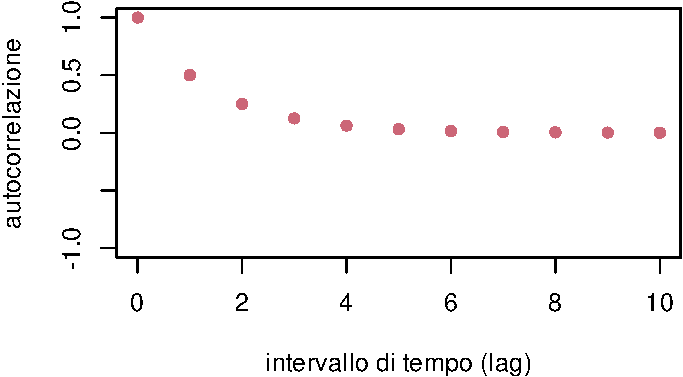
\includegraphics[keepaspectratio]{07-processi_continui_files/figure-pdf/unnamed-chunk-2-1.pdf}}

}

\caption{funzione di autocorrelazione dell'equazione lineare con
smorzamento per \(\alpha=1/2\)}

\end{figure}%

\begin{Shaded}
\begin{Highlighting}[]
\NormalTok{t }\OtherTok{=} \DecValTok{0}\SpecialCharTok{:}\DecValTok{10}
\NormalTok{alpha }\OtherTok{=} \SpecialCharTok{{-}}\DecValTok{1}\SpecialCharTok{/}\DecValTok{2}

\FunctionTok{plot}\NormalTok{(t, alpha}\SpecialCharTok{\^{}}\NormalTok{t, }\AttributeTok{pch=}\DecValTok{16}\NormalTok{, }\AttributeTok{lwd=}\DecValTok{3}\NormalTok{, }\AttributeTok{col=}\NormalTok{miei\_colori[}\DecValTok{2}\NormalTok{], }\AttributeTok{ylab=}\StringTok{\textquotesingle{}autocorrelazione\textquotesingle{}}\NormalTok{, }\AttributeTok{xlab=}\StringTok{\textquotesingle{}intervallo di tempo (lag)\textquotesingle{}}\NormalTok{, }\AttributeTok{ylim=}\FunctionTok{c}\NormalTok{(}\SpecialCharTok{{-}}\DecValTok{1}\NormalTok{,}\DecValTok{1}\NormalTok{) )}
\end{Highlighting}
\end{Shaded}

\begin{figure}[H]

{\centering \pandocbounded{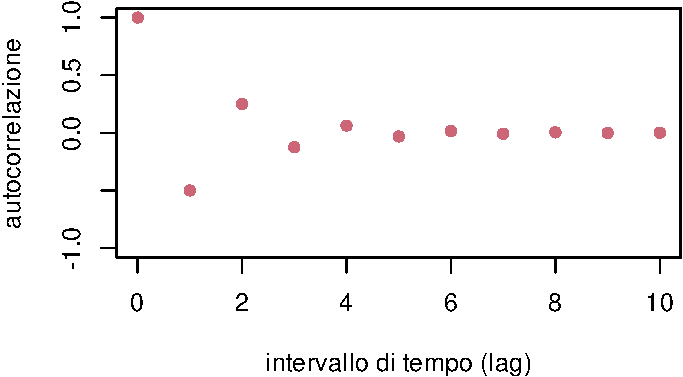
\includegraphics[keepaspectratio]{07-processi_continui_files/figure-pdf/unnamed-chunk-3-1.pdf}}

}

\caption{funzione di autocorrelazione dell'equazione lineare con
smorzamento per \(\alpha=-1/2\)}

\end{figure}%

\begin{remark}
Se i parametri \(\alpha\) e \(\sigma^2\) non sono noti, si possono
stimare da \(n\) osservazioni \(X_t = x_t\) per \(t = 0,1, \ldots, n\).
Similmente a quanto visto per la passeggiata aleatoria, ci possiamo
ricondurre ad \(n\) osservazioni di rumore bianco gaussiano tramite le
differenze \[ w_t = x_t - \alpha x_{t-1}.\] La funzione di
verosimiglianza per il rumore bianco è molto semplice (essendo gaussiane
indipendenti) e si trova quindi
\[\begin{split} L( \alpha, \sigma^2 ; (x_t)_{t=0}^n)  & = p( W_t= x_t-\alpha x_{t-1},  \ldots, W_1 = x_1 - \alpha x_0 | \alpha, \sigma^2)\\ 
& = \exp\bra{ - \frac 1 2  \sum_{t=1}^n \frac{ (x_t - \alpha x_{t-1})^2 }{\sigma^2 } } \frac {1}{\sqrt{ (2 \pi )^n \sigma^{2n}}}
\end{split}\] Con i soliti passaggi si riconduce la stima di massima
verosimiglianza a minimizzare la funzione congiunta di \(\alpha\) e
\(\sigma^2\),
\[    \sum_{t=1}^n \frac{ (x_t - \alpha x_{t-1})^2 }{\sigma^2 }   - n \log( \sigma^2)\]
In particolare, \(\alpha_{\mle}\) minimizza la somma dei quadrati dei
``residui'' \[ \alpha \mapsto \sum_{t=1}^n (x_t - \alpha x_{t-1})^2,\] e
quindi, imponendo che la derivata si annulli,
\[ \alpha_{\mle}  = \frac{\sum_{t=1}^n x_t x_{t-1}}{ \sum_{t=1}^n x_{t-1}^2} \]
mentre \(\sigma_{\mle}^2\) si ottiene di conseguenza
\[ \sigma_{\mle}^2 = \frac 1 n  \sum_{t=1}^n (x_t - \alpha_{\mle} x_{t-1})^2.\]
\end{remark}

\subsection{Esercizi}\label{esercizi-39}

Trovare la stima di massima verosimiglianza per \(\sigma^2\) quando si
osserva una passeggiata aleatoria gaussiana a istanti di tempo non
costanti \(0\le t_1 < t_2 < \ldots < t_n\).

\section{Modelli ARIMA: definizione}\label{sec-arima-def}

In questa sezione generalizziamo gli esempi visti sopra introducendo una
famiglia generale di processi, detti ARIMA, che è una abbreviazione per
l'espressione inglese \textbf{A}uto\textbf{R}egressive
\textbf{I}ntegrated \textbf{M}oving \textbf{A}verage (in italiano,
autoregressivi integrati a media mobile). Come vedremo sono piuttosto
semplici da parametrizzare ma risultano flessibili e utili per
l'inferenza sui processi (in particolare la previsione dei valori futuri
a partire dall'osservazione di una serie storica).

Per arrivare alla definizione generale conviene studiare separatamente i
tre ``ingredienti'' principali che vanno a comporre un processo ARIMA, e
precisamente la componente autoregressiva (AR), quella a media mobile
(MA) e il procedimento di integrazione (I) a tempi discreti.

In tutta questa sezione supporremo che
\(\mathcal{T} = \cur{0,1, \ldots, n}\) oppure \(\mathcal{T} = \N\) o
anche \(\mathcal{T} = \mathbb{Z}\), e che \((W_t)_{t \in \mathcal{T}}\)
sia un rumore bianco gaussiano di intensità \(\sigma^2\).

Introduciamo anche l'operatore di ritardo (lag) \(L\) che trasforma un
processo \((X_t)_{t \in \mathcal{T}}\) in \((LX)_t = X_{t-1}\) (pensato
come processo sui tempi \(t \ge 1\) se
\(\mathcal{T} = \cur{0,1, \ldots, n}\) oppure \(\mathbb{N}\)). Spesso,
per alleggerire la notazione, scriviamo semplicemente \(LX_t\) invece di
\((LX)_t\).

L'operatore \(L\) è lineare:
\[ L(X+Y)_t = X_{t-1}+Y_{t-1} = LX_t + LY_t, \quad L(c X)_t = c LX_t.\]
inoltre componendo \(L\) con se stesso si ottengono ritardi di ordine
superiore: \(L^2X_t = LLX_t = X_{t-2}\), \(L^3X_t = X_{t-3}\), ecc. Il
vantaggio di questa notazione è che espressioni del tipo
\[ a_0 X_t + a_1 X_{t-1}+ \ldots +a_k X_{t-k} = a_0  X_t + a_1LX_t +a_2 L^2 X_t + \ldots a_k L^k X_t\]
si possono pensare come all'azione di un polinomio (formale) nella
variabile \(L\), precisamente
\[p(L) X_t  =  (a_0   + a_1L +a_2 L^2 + \ldots a_k L^k ) X_t.\] Vedremo
infatti che i modelli ARIMA si descrivono agevolmente usando polinomi di
questo tipo.

\subsection{Modelli AR}\label{modelli-ar}

I modelli autoregressivi generalizzano il caso dell'equazione lineare
con smorzamento della sezione precedente. L'osservazione di base è che
l'equazione \[ X_t = \alpha X_{t-1} + W_t\] può essere pensata in
termini di regressione lineare semplice, cui la variabile del processo
\(X_t\) è stimata a partire dallo stesso processo, ma con ritardo, ossia
\(X_{t-1}\) (da cui il termine \emph{autoregressivo}). L'idea è quindi
di estendere al caso di una regressione lineare multipla, su \(p \ge 1\)
istanti precedenti.

Dato \(p \ge 0\), un processo \((X_t)_{t \in \mathcal{T}}\) è detto
\(\operatorname{AR}(p)\) (autoregressivo di ordine \(p\)) se esistono
parametri \(\alpha_1, \alpha_2, \ldots, \alpha_p \in \R\) tali che, per
ogni \(t \in \mathcal{T}\) (tale che \(t-p \in \mathcal{T}\)) si abbia
\[ X_t = \alpha_1 X_{t-1} + \alpha_2 X_{t-2}+ \ldots + \alpha_p X_{t-p } +W_t.\]

Usando l'operatore \(L\) si può riscrivere l'equazione del modello
\(\operatorname{AR}(p)\) nel seguente modo compatto:
\[ p(L) X_t = W_t,\] dove \(p(L)\) è il polinomio formale nella
variabile \(L\) dato da
\[ p(L) = 1- \alpha_1L -\alpha_2L ^2 - \ldots  - \alpha_p L^p = 1 - \sum_{i=1}^p \alpha_i L^i.\]

\subsection{Modelli MA}\label{modelli-ma}

Vediamo ora il secondo ``ingrediente'', ossia la componente a media
mobile (\emph{moving average} in inglese, MA). Il punto di partenza
stavolta è l'operazione elementare di media mobile su una finestra
temporale sinistra di ampiezza \(q \ge 1\), in cui ad un processo
\((Z_t)_{t \in \mathcal{T}}\) (o alle sue osservazioni) si sostituiscono
le medie \[ \bar{Z}_t = \frac 1 q \sum_{i=0}^{q-1} Z_{t-i}.\] Osserviamo
che si tratta di un caso particolare di \emph{convoluzione} \(Z * g\)
tra il processo e il filtro
\[ g (t ) = \begin{cases} \frac 1 q & \text{se $i=0,1, \ldots, (q-1)$}\\
 0 & \text{altrimenti.}\end{cases}
 \]

\begin{remark}
Notiamo che, qualsiasi sia \(g\) (nota e fissata), se il processo \(Z\)
è stazionario (in senso lato o anche in senso stretto), anche \(Z * g\)
lo è (nello stesso senso). Ad esempio, la funzione di media è data da
\[\E{ (Z * g)_t} = \E{ \sum_i Z_{t-1} g(i)} =  \sum_i \E{Z_{t-1} } g(i) = m \sum_i g(i),\]
avendo indicato con \(m = \E{Z_s}\). La funzione di autocovariaza è,
usando la bilinearità,
\[ \begin{split} C(s,t) & = \Cov{ (Z * g)_s, (Z*g)_t} = \sum_{i} \sum_j g(i) g(j) \Cov{Z_{s-i}, Z_{t-j}}\\
&= \sum_{i} \sum_j g(i) g(j) C( (t-s) + (i-j))
\end{split}\] che dipende da \(s,t\) solamente tramite la differenza.
Inoltre, se \(Z\) è un processo gaussiano, anche \(Z*g\) lo è, perché è
una trasformazione lineare di \(Z\).
\end{remark}

Vediamo quindi la definizione dei processi a media mobile.

Dato \(q \ge 0\), un processo \((X_t)_{t \in \mathcal{T}}\) è detto
\(\operatorname{MA}(p)\) (a media mobile di ordine \(q\)) se esistono
parametri \(\beta_1, \beta_2, \ldots, \beta_q \in \R\) tali che, per
ogni \(t \in \mathcal{T}\) (tale che \(t-q \in \mathcal{T}\)) si abbia
\[ X_t = W_t + \beta_1 W_{t-1} + \beta_2 W_{t-2}+ \ldots + \beta_q W_{t-q }.\]

Per quanto osservato sopra, un processo a media mobile
\(\operatorname{MA}(q)\) è semplicemente del tipo \(W * g\), dove \(g\)
è dato dai coefficienti \(1\), \(\beta_1\), \(\beta_2\), \ldots,
\(\beta_q\) (e nullo altrove). In particolare, \(X\) è gaussiano e
stazionario (perché lo è il rumore bianco gaussiano).

Una notazione compatta usa anche in questo caso un polinomio
dell'operatore ritardo: \[ X_t = q(L)W_t,\] dove
\[ q(L ) = 1 + \beta_1 L + \ldots + \beta_q L^q = 1 + \sum_{j=1}^q \beta_q L^j.\]

\subsection{Integrazione discreta}\label{integrazione-discreta}

Presentiamo infine l'operazione di integrazione (I) a tempi discreti.
Per introdurla conviene considerare prima l'operazione di derivazione,
in cui l'idea è che la derivata di un processo
\((X_t)_{t\in \mathcal{T}}\) a tempi discreti diventa la differenza
finita \[ X_t - X_{t-1} = (1-L)X_t,\] per \(t \ge 1\). Iterando per
ottenere l'analogo discreto delle derivate di ordine superiore si trova
che la derivata di ordine \(d\) corrisponde a
\[ (1-L)^d X_t = \sum_{i=0}^d { d \choose i} (-1)^i L^i X_t.\] La
formula sopra si può anche pensare ad una convoluzione \(X * g\), dove
\(g(i) = { d \choose i} (-1)^i\). Pertanto se \(X\) è stazionario, lo è
anche ogni derivata discreta di qualsiasi ordine \(d\).

L'operazione di integrazione discreta è l'inversa della derivata
discreta, e quindi diremo che \(X\) è l'integrale discreto di \(Y\) se
\((1-L)X = Y\), e similmente se vogliamo considerare integrali iterati
\(d\) volte, dovrà valere \((1-L)^d X = Y\).

Abbiamo già incontrato un esempio di processo ottenuto tramite
integrazione discreta: è la passeggiata aleatoria gaussiana,
\(S_t = S_{t-1} + W_t\), che si può riscrivere anche come
\[ (1-L) S _t  =W_t.\] Questo esempio mostra anche che in generale
l'integrazione discreta non mantiene la stazionarietà di un processo.

\subsection{Definizione generale}\label{definizione-generale}

Mettendo insieme i tre elementi visti sopra, diamo la definizione
generale di un processo ARIMA.

Dati \(p, d, q \ge 0\), un processo \((X_t)_{t \in \mathcal{T}}\) è
detto \(\operatorname{ARIMA}(p,d,q)\) se esistono parametri
\((\alpha_i)_{i=1}^p\), \((\beta_j)_{j=1}^q\) reali tali che, per ogni
\(t \in \mathcal{T}\) (tale che \(t-d-p\) e \(t-q \in \mathcal{T}\)),
posto \[ Y_t  = (1-L)^d X_t\] valga
\[ Y_t = \sum_{i=1}^p \alpha_i Y_{t-i} + W_t + \sum_{j=1}^q  \beta_j W_{t-j}.\]

Usando i polinomi
\[ p(L) = 1- \sum_{i=1}^ p \alpha_i L^i, \quad \text{e } \quad q(L) = 1+ \sum_{j=1}^q \beta_j L^j\]
si può scrivere in forma compatta la definizione sopra nel seguente
modo: \[ p(L)(1-L)^d X_t = q(L)W_t.\]

Con questa definizione, il rumore bianco gaussiano è
\(\operatorname{ARIMA}(0,0,0)\), mentre la passeggiata aleatoria è
\(\operatorname{ARIMA}(0,1,0)\), e l'equazione lineare con smorzamento
definisce un processo \(\operatorname{ARIMA}(1,0,0)\).

\begin{remark}
Spesso una caratteristica dei dati osservati è di presentare una
``periodicità approssimata'', o \emph{stagionalità} dovuta ad esempio,
ma non necessariamente, a cause cicliche, si pensi a fenomeni come la
produzione agricola di un terreno o i livelli di acqua mensili
registrati in un lago. Anche se non è necessario, è possibile
specificare una struttura nell'equazione definente un modello ARIMA per
tenere conto della stagionalità. Supponiamo infatti che il periodo
consista di \(s\) unità di tempo: allora si può imporre che, per
ulteriori polinomi \(P(L^s)\), \(Q(L^s\), di gradi rispettivamente \(P\)
e \(Q\) e per \(D \ge 1\) l'equazione sia del tipo
\[  P(L^s) (1-L^s)^D p(L)(1-L)^d X_ t = Q(L^s) P(L^s) W_t. \] Un tale
processo è indicato anche come
\(\operatorname{SARIMA}(p,d,q)(P,D,Q)_s\). Anche se in apparenza il
numero dei parametri cresce, questa parametrizzazione può essere più
efficace di considerare semplicemente un modello ARIMA con \(p\), \(d\),
\(q\) molto grandi (in modo da includere gli effetti dovuti alla
stagionalità).
\end{remark}

\section{Modelli ARIMA: proprietà}\label{sec-arima-prop}

In questa sezione discutiamo tre proprietà fondamentali dei modelli
ARIMA, ottenendo condizioni sulla stazionarietà, una equazione ricorsiva
per la funzione di autocovarianza (nel caso stazionario) e infine
accennando al problema della stima dei parametri sulla base delle
osservazioni, che include anche il problema della selezione del modello,
ossia la scelta degli ordini \((p,d,q)\).

Consideriamo quindi un processo \((X_t)_{t \in \mathcal{T}}\)
\(\operatorname{ARIMA}(p,d,q)\) di parametri \((\alpha_i)_{i=1}^p\) e
\((\beta_j)_{j=1}^q\).

\subsection{Stazionarietà}\label{stazionarietuxe0}

Il problema della stazionarietà è stato discusso nel caso
\(\operatorname{ARIMA}(1,0,0)\), l'equazione lineare con smorzamento, in
cui era stata ottenuta la condizione necessaria \(|\alpha_1| <1\) (e
sufficiente, purché \(X_0\) fosse gaussiano di varianza opportuna).
L'esempio della passeggiata aleatoria, pensato come
\(\operatorname{ARIMA}(0,1,0)\) mostra che in tal caso la stazionarietà
non vale.

Prima di presentare il risultato generale, osserviamo che i processi a
media mobile, ossia \(\operatorname{ARIMA}(0,0,q)\) possono sempre
essere stazionari (se si definiscono \(X_0\), \(X_1\), \ldots,
\(X_{q-1}\) opportunamente). Infatti l'equazione che li definisce,
\[ X_t = q(L) W_t = W_t + \beta_1 W_{t-1} + \beta_2 W_{t-2} + \ldots + \beta_q W_{t-q}\]
se estesa anche per \(t = 0\), \(1\), \ldots, \(q-1\) considerando il
rumore bianco gaussiano definito anche per tempi negativi, è un caso
particolare di convoluzione di un processo stazionario (il rumore bianco
gaussiano \(W\)) con un filtro (dato dai coefficienti \(\beta_j\)), e
quindi abbiamo già osservato che preserva la stazionarietà.

Per comprendere la stazionarietà nel caso generale, l'idea formale è di
``risolvere'' l'equazione del modello \[ p(L)(1-L)^d X_t = q(L) W_t,\]
dividendo formalmente per \(p(L)(1-L)^d\). Si ottiene
\[ X_ t =\frac{ q(L)}{ p(L)(1-L)^d} W_t,\] una scrittura che però non ha
molto senso (sappiamo definire solo i polinomi nell'operatore ritardo
\(L\), non certo le funzioni razionali). Tuttavia, sviluppando la
funzione come serie di Taylor
\[ \frac{ q(z)}{p(z)(1-z)^d}  = \sum_{k=0}^\infty b_k z^k,\] possiamo
almeno tentare di definire \(X\) nel seguente modo,
\[ X_t = \sum_{k=0}^\infty b_k L^k W_t,\] avendo definito \(W_t\) anche
per \(t\) negativi, che è una sorta di modello a media mobile con
\(q=\infty\). La stazionarietà sarebbe allora un caso limite di quanto
osservato prima, per \(q\) finito. Ovviamente tutto il problema sta nel
mostrare che la serie effettivamente converge, fatto che dipende dalla
crescita dei coefficienti \(b_k\) al tendere di \(k \to \infty\) e in
ultima analisi agli zeri (complessi) del denominatore \(p(z)(1-z)^d\).
Il risultato preciso che si può dimostrare è il seguente.

Dati \((p,d,q)\) e coefficienti \((\alpha_i)_{i=1}^p\),
\((\beta_j)_{j=1}^q\), posto \[ p(z) = 1- \sum_{i=1}^p \alpha_i z^i,\]
allora esiste un modello \(\operatorname{ARIMA}(p,d,q)\) stazionario con
tali coefficienti se \(d=0\) e tutte le radici complesse di \(p(z)\)
hanno modulo \(|z|>1\), ossia
\[ \text{se $z \in \mathbb{C}$  è tale che $p(z) = 0$, allora $|z|>1$.}\]

Verifichiamo che il teorema recupera la condizione trovata per
l'equazione lineare con smorzamento. In tal caso vale
\[ p(z) =1 -\alpha_1 z,\] la cui unica radice è \(z = 1/\alpha_1\). Essa
ha modulo maggiore di \(1\) se e solo se \(|\alpha_1|<1\), che è appunto
la condizione trovata.

\subsection{Autocovarianza}\label{autocovarianza}

Per costruzione i processi ARIMA hanno media nulla (nel caso fosse
rilevante ammettere una media \(m\) non nulla basta modellizzare la
differenza \(X_t - m\) come un ARIMA). L'equazione permette anche di
ottenere una formula ricorsiva per la funzione di autocovarianza.

Vale infatti (supponiamo \(d=0\) per semplicità), per
\(t\ge \max\cur{p,q}\),
\[  \E{ X_s p(L) X_t} = \E{ X_s q(L) W_t} = \E{ X_s (W_t+\sum_{j=1}^q \beta_j W_{t-j})}\]
Possiamo supporre che \(X_s\) sia indipendente dal rumore bianco
\(W_r\), purché \(r>s\). In particolare, se \(t-q >s\), il membro a
destra contiene solamente termini nulli, perché del tipo
\[ \E{ X_s W_r}\] con \(r>s\). Ne segue che
\[ 0 =  \E{ X_s p(L) X_t } = \E{ X_s (X_t - \sum_{i=1}^p \alpha_i X_{t-i} )} = C(s,t)-\sum_{i=1}^p \alpha_i C(s,t-i).\]
Riorganizzando i termini, troviamo che
\[ C(s,t) = \sum_{i=1}^p \alpha_i C(s, t-i),\] purché \(t > s +q\). In
particolare,
\[ C(0,t) = \sum_{i=1}^p \alpha_i C(0, t-i), \quad \text{se $t>q$.}\]
che è particolarmente utile nel caso in cui \(X\) sia stazionario.

Queste formule ricorsive sono dette \emph{equazioni di Yule-Walker} e
permettono di ricavare la funzione di autocovarianza per intervalli
temporali (lag) grandi. In particolare, notiamo che nel caso \(p=1\), si
riduce alla relazione già trovata \[ C(0,t) = \alpha_1 C(0,t-1)\] che
iterando porta a \[ C(0,t) = \alpha_1^t C(0,0).\] Recuperiamo il fatto
che la funzione diventa esponenzialmente piccola (nel caso stazionario
\(|\alpha_1|<1\)) al crescere di \(t\). Questo fatto vale più in
generale per processi \(\operatorname{ARIMA}\) stazionari. Un caso
``limite'' è quello dei processi a media mobile, ossia
\(\operatorname{ARIMA}(0,0,q)\). In questo caso \(\alpha_i = 0\) e
quindi \[ C(0,t) = 0\] è identicamente nulla se \(t>q\).

\subsection{Stima dei parametri}\label{stima-dei-parametri}

A partire dall'osservazione di una serie storica \((x_t)_{t=0}^n\), come
stimare i parametri di un processo ARIMA che la descrivono nel modo
migliore? Abbiamo già osservato che la stima di massima verosimiglianza
può fornire una risposta nel caso del rumore bianco gaussiano, della
passeggiata aleatoria e dell'equazione lineare con smorzamento. In tutti
e tre i casi il metodo si riduce alla minimizzazione dei residui
quadratici (che appunto sono per ipotesi gaussiane indipendenti).

Si può quindi proporre lo stesso per un modello generale, dove tuttavia
la nozione di residuo va chiarita, perché dall'equazione
\[ p(L)(1-L)^d X_t = q(L)W_t\] è necessario ricavare il rumore bianco
gaussiano \(W_t\), scrivendo
\[ W_t = - \sum_{j=1}^q \beta_j W_{t-j} +p(L)(1-L)^dX_t\] Supponendo di
osservare \(X_t = x_t\), questa equazione permette di definire
ricorsivamente i residui
\[ w_t = - \sum_{j=1}^q \beta_j w_{t-j} + p(L)(1-L)^d x_t,\] da cui
infine la stima di massima verosimiglianza si ottiene minimizzando i
residui quadratici (come funzione dei coefficienti
\(\alpha = (\alpha_i)_{i=1}^p\) e \(\beta = (\beta_j)_{j=1}^q)\):
\[ (\alpha_{\mle}, \beta_{\mle}) \in \operatorname{arg} \min_{\alpha, \beta} \sum_{t} w_t^2\]
Per la risoluzione ci affidiamo a metodi numerici (in particolare se
\(q\neq 0\)).

\begin{remark}
In R la funzione \texttt{arima()} oppure la funzione \texttt{Arima()}
dalla libreria \texttt{forecast} permette di stimare i coefficienti di
un modello arima (di ordine specificato) a partire dalle osservazioni.
Avendo stimato i coefficienti la funzione \texttt{forecast()} permette
anche di ottenere delle stime sui valori futuri come previsti dalle
equazioni ricorsive del modello (con i coefficienti stimati)
accompagnate da stime dell'incertezza (deviazione standard) dovute al
termine di rumore bianco gaussiano.
\end{remark}

La stima dei coefficienti non esaurisce tuttavia il problema, perché
rimane da determinare l'ordine del modello, ossia la tripla di numeri
\((p,d,q)\). È chiaro che, più grandi sono \(p\) e \(q\), più
coefficienti avremo a disposizione e migliore sarà l'aderenza del
modello ai dati osservati. Tuttavia, con una eccessiva aderenza si
potrebbe incappare nel problema dell'overfit, e quindi non ottenere ad
esempio previsioni ragionevoli. Per questo ci si serve di indicatori che
tengano conto di tali fenomeni, come ad esempio gli indici AIC o BIC,
utili per confrontare diversi modelli (sono da preferire i modelli con
indici più piccolo). La libreria R \texttt{forecast} contiene il comando
\texttt{auto.arima()} che restituisce automaticamente il \emph{miglior
modello} ARIMA a partire dai dati osservati e usando uno di questi
criteri.

Consideriamo il dataset precaricato in R \texttt{AirPassengers} che
raccoglie una serie storica con i dati relativi al numero di passeggeri
nelle linee aree internazionali dal 1949 al 1960. Usiamo i comandi
descritti sopra sul modello.

\begin{Shaded}
\begin{Highlighting}[]
\FunctionTok{plot}\NormalTok{(AirPassengers, }\AttributeTok{lwd=}\DecValTok{3}\NormalTok{, }\AttributeTok{col=}\NormalTok{miei\_colori[}\DecValTok{2}\NormalTok{])}
\end{Highlighting}
\end{Shaded}

\begin{figure}[H]

{\centering \pandocbounded{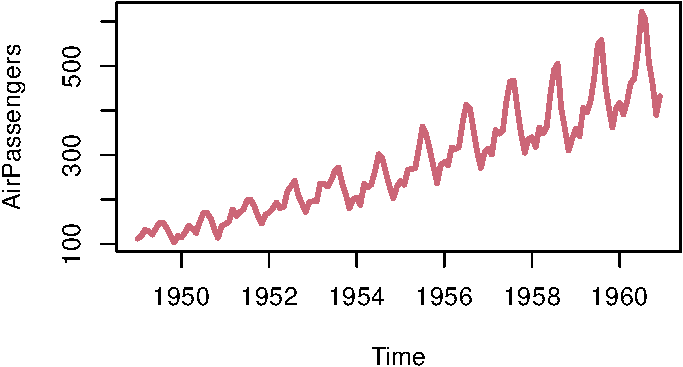
\includegraphics[keepaspectratio]{07-processi_continui_files/figure-pdf/unnamed-chunk-4-1.pdf}}

}

\caption{Grafico della serie storica considerata}

\end{figure}%

\begin{Shaded}
\begin{Highlighting}[]
\CommentTok{\# Usiamo direttamente il comando auto.arima dalla libreria \textquotesingle{}forecast\textquotesingle{}}

\FunctionTok{library}\NormalTok{(}\StringTok{\textquotesingle{}forecast\textquotesingle{}}\NormalTok{)}

\NormalTok{AP\_auto }\OtherTok{=} \FunctionTok{auto.arima}\NormalTok{(AirPassengers)}

\CommentTok{\# Con la funzione summary() possiamo vedere le informazioni principali}

\FunctionTok{summary}\NormalTok{(AP\_auto)}
\end{Highlighting}
\end{Shaded}

\begin{verbatim}
Series: AirPassengers 
ARIMA(2,1,1)(0,1,0)[12] 

Coefficients:
         ar1     ar2      ma1
      0.5960  0.2143  -0.9819
s.e.  0.0888  0.0880   0.0292

sigma^2 = 132.3:  log likelihood = -504.92
AIC=1017.85   AICc=1018.17   BIC=1029.35

Training set error measures:
                   ME     RMSE      MAE       MPE     MAPE
Training set 1.342306 10.84619 7.867539 0.4206996 2.800458
                 MASE         ACF1
Training set 0.245628 -0.001248451
\end{verbatim}

Vediamo che la funzione \texttt{auto.arima()} propone un modello ARIMA
con stagionalità di periodo \(12\) (mesi) e ordine \((2,1,1)(0,1,0)\)
(la seconda tripla si riferisce alla stagionalità). Precisamente, la
funzione \texttt{auto.arima()} non determina automaticamente il periodo
\(12\) e questo va indicato prima di applicarla ai dati, nel momento in
cui si definisce un oggetto di tipo \emph{serie storica} (in inglese
\emph{time series}) in R. Partendo da un vettore di dati osservati, il
comando è \texttt{ts()}, che contiene l'opzione \emph{frequency} (se non
specificata è posta uguale ad \(1\)). In generale si può ricorrere alla
funzione di autocorrelazione empirica (vedere la sezione successiva) o
ad analisi spettrale per determinare eventuali stagionalità e il loro
periodo. Un comando automatico è \texttt{findfrequency()}.

\begin{Shaded}
\begin{Highlighting}[]
\CommentTok{\# Con la funzione forecast() possiamo effettuare semplici previsioni per un numero di mesi futuri specificato}

\NormalTok{previsione }\OtherTok{=} \FunctionTok{forecast}\NormalTok{(AP\_auto, }\DecValTok{24}\NormalTok{)}

\CommentTok{\# La funzione plot() si occupa di rappresentare sia i dati osservati che la previsione (e pure le bande di errore date dalle deviazioni standard stimate)}

\FunctionTok{plot}\NormalTok{(previsione, }\AttributeTok{xlab=}\StringTok{\textquotesingle{}anno\textquotesingle{}}\NormalTok{, }\AttributeTok{ylab=}\StringTok{\textquotesingle{}numero passeggeri\textquotesingle{}}\NormalTok{, }\AttributeTok{col=}\NormalTok{miei\_colori[}\DecValTok{2}\NormalTok{], }\AttributeTok{lwd=}\DecValTok{3}\NormalTok{)}
\end{Highlighting}
\end{Shaded}

\begin{figure}[H]

{\centering \pandocbounded{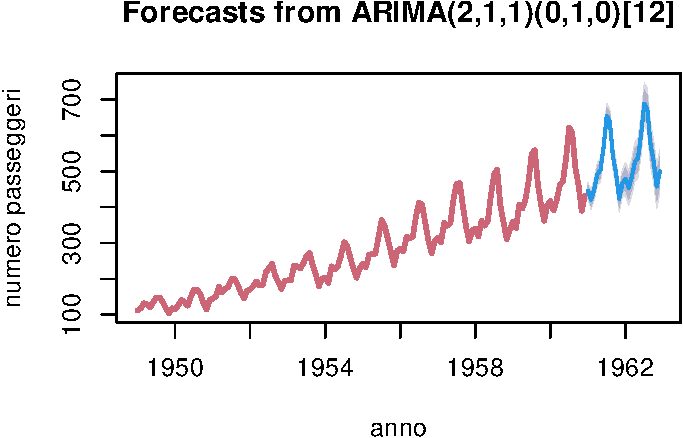
\includegraphics[keepaspectratio]{07-processi_continui_files/figure-pdf/unnamed-chunk-6-1.pdf}}

}

\caption{dati osservati e previsione con un modello SARIMA}

\end{figure}%

Come in molti altri problemi di stima, particolare attenzione va
prestata alla gaussianità dei residui, pure forniti dalla funzione
\texttt{auto.arima()}.

\begin{Shaded}
\begin{Highlighting}[]
\FunctionTok{par}\NormalTok{(}\AttributeTok{mfrow=}\FunctionTok{c}\NormalTok{(}\DecValTok{1}\NormalTok{,}\DecValTok{2}\NormalTok{))}

\FunctionTok{hist}\NormalTok{(AP\_auto}\SpecialCharTok{$}\NormalTok{residuals, }\AttributeTok{col=}\NormalTok{miei\_colori[}\DecValTok{1}\NormalTok{], }\AttributeTok{freq=}\ConstantTok{FALSE}\NormalTok{, }\AttributeTok{xlab=}\StringTok{\textquotesingle{}residui\textquotesingle{}}\NormalTok{, }\AttributeTok{ylab=}\StringTok{\textquotesingle{}frequenze\textquotesingle{}}\NormalTok{, }\AttributeTok{main=}\StringTok{"istogramma dei residui"}\NormalTok{)}
\NormalTok{valori }\OtherTok{=} \FunctionTok{seq}\NormalTok{(}\FunctionTok{min}\NormalTok{(AP\_auto}\SpecialCharTok{$}\NormalTok{residuals), }\FunctionTok{max}\NormalTok{(AP\_auto}\SpecialCharTok{$}\NormalTok{residuals), }\AttributeTok{by=}\FloatTok{0.1}\NormalTok{)}
\FunctionTok{lines}\NormalTok{( valori, }\FunctionTok{dnorm}\NormalTok{(valori , }\AttributeTok{mean=}\FunctionTok{mean}\NormalTok{(AP\_auto}\SpecialCharTok{$}\NormalTok{residuals), }\AttributeTok{sd=}\FunctionTok{sd}\NormalTok{(AP\_auto}\SpecialCharTok{$}\NormalTok{residuals)), }\AttributeTok{col=}\NormalTok{miei\_colori[}\DecValTok{2}\NormalTok{], }\AttributeTok{lwd=}\DecValTok{3}\NormalTok{)}

\FunctionTok{qqnorm}\NormalTok{(AP\_auto}\SpecialCharTok{$}\NormalTok{residuals, }\AttributeTok{col=}\NormalTok{miei\_colori[}\DecValTok{1}\NormalTok{], }\AttributeTok{pch=}\DecValTok{16}\NormalTok{)}
\FunctionTok{qqline}\NormalTok{(AP\_auto}\SpecialCharTok{$}\NormalTok{residuals, }\AttributeTok{col=}\NormalTok{miei\_colori[}\DecValTok{2}\NormalTok{], }\AttributeTok{lwd=}\DecValTok{3}\NormalTok{)}
\end{Highlighting}
\end{Shaded}

\begin{figure}[H]

{\centering \pandocbounded{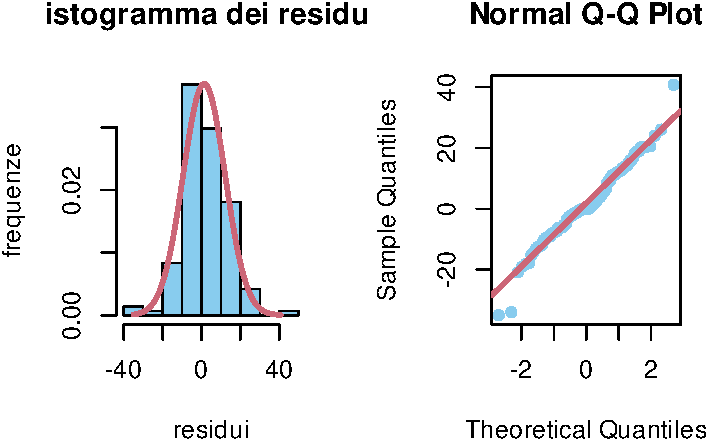
\includegraphics[keepaspectratio]{07-processi_continui_files/figure-pdf/unnamed-chunk-7-1.pdf}}

}

\caption{istogramma e QQ-plot dei residui}

\end{figure}%

\section{Stima della funzione di
autocovarianza}\label{sec-wiener-kinchin}

In questa sezione affrontiamo il problema generale di stimare la
funzione di media e di autocovarianza di un processo \(X\) a partire
dall'osservazione dei valori per \(n\) tempi consecutivi
\((X_t)_{t=0}^{n-1} = (x_t)_{t=0}^{n-1}\), anche detta nel linguaggio
statistico una \emph{serie storica}.

Si può pensare a questo problema come ad una generalizzazione del
problema di stimare valor medio e varianza di una famiglia di variabili
aleatorie indipendenti, tutte con la stessa legge. In particolare,
abbiamo affrontato il caso gaussiano nella Sezione
Sezione~\ref{sec-stimaindipendenti} e ottenuto come stime di massima
verosimiglianza la media e la covarianza campionarie.

In questo caso introduciamo, invece dell'ipotesi di indipendenza, la
stazionarietà del processo, ossia la matrice di covarianza delle
variabili \((X_t)_{t =0}^{n-1}\) è costante sulle diagonali (oltre ad
essere simmetrica):
\[ (C(s,t))_{s,t=0}^{n-1} = (C(|t-s|))_{s,t=0}^{n-1}\] e supponiamo pure
che il processo \(X\) sia gaussiano e centrato (ossia la funzione di
media sia nota e costantemente nulla): in questo modo possiamo scrivere
esplicitamente la funzione di verosimiglianza (supponendo che la matrice
di covarianza sia invertibile)
\[\begin{split} L( C ; x) & = p((X_t)_{t=0}^{n-1} = (x_t)_{t=0}^{n-1} |  C) \\
& \propto \exp\bra{ - \frac 1 2 x^T C^{-1} x} \frac{1}{\sqrt{ \det C }},\end{split}\]
dove abbiamo posto, per alleggerire la notazione,
\(x = (x_t)_{t=0}^{n-1}\).

Possiamo determinare la stima di massima verosimiglianza per \(C\) con i
soliti passaggi, ossia passando al logaritmo e cambiando di segno: si
tratta di minimizzare la funzione
\[ C \mapsto x^T C^{-1} x + \log \det C.\] Tuttavia è comunque difficile
calcolare esplicitamente \(C_{\mle}\) (ma si può ricorrere a metodi
numerici).

Per proseguire analiticamente e ottenere delle espressioni elementari
conviene introdurre una ulteriore ipotesi matematica nella struttura
della matrice di covarianza: non solo supponiamo che sia costante sulle
diagonali, ma anche che sia \emph{circolante}, ossia che valga
l'identità, per ogni \(k =1,2,\ldots, n-1\), \[ C(k) = C(n-k).\] Questa
ipotesi è giustificabile solo per semplificare i calcoli, non vi è una
ragione particolare per ritenere che la funzione di autocovarianza di un
processo stazionario la soddisfi, eccetto al più nel caso in cui il
processo sia periodico di periodo \(n\), ossia valga \(X_{t+n} = X_t\)
per ogni \(t\). Ma ricordiamo che \(n\) è solamente il numero di
osservazioni, e di solito se vi è una periodicità, anche approssimata
(si parla in tal caso di una \emph{stagionalità}) essa è di periodo
molto minore di \(n\). In ogni caso, una volta trovata \(C_{\mle}\) con
questa ipotesi, possiamo proporre una modifica per il caso generale.
Un'altra possibilità sarebbe di ragionare nel limite \(n \to \infty\),
ma quento introdurrebbe ulteriori problemi tecnici.

Il vantaggio di supporre che la matrice \(C\) sia circolante è che,
passando alla trasformata di Fourier a tempi finiti, essa diventa
diagonale. Precisamente, usando la notazione della Sezione
Sezione~\ref{sec-fourier-finita}, introduciamo la matrice
\(F \in \mathbb{C}^{n\times n}\), \[ F_{\xi t} = e^{-2 \pi i \xi t/n},\]
per \(\xi = 0,1, \ldots, (n-1)\), in modo che la trasformata di Fourier
a tempi finiti di \((x_t)_{t =0}^{n-1}\) sia
\[\hat x (\xi ) = \sum_{t=0}^{n-1} x_t e^{- 2 \pi i \xi t/n} = \sum_{t=0}^{n-1} F_{\xi t} x_t,\]
ossia \(\hat x = F x\). Ricordando che \(x\) è l'osservazione del
processo \(X\), la matrice di covarianza del vettore aleatorio \(FX\) si
trasforma come al solito (formula per le trasformazioni affini)
\[ \Sigma_{ FX} =  F \Sigma_X \bar{F}^T = FC \bar{F}^T,\] dove l'unico
accorgimento è che, essendo la matrice \(F\) complessa, la formula va
modificata introducendo il coniugato del trasposto \(\bar{F}^T\) (invece
del semplice trasposto).

Questo cambio di coordinate dalla base dei ``tempi'' a quella delle
``frequenze'' ha l'effetto di diagonalizzare la matrice delle
covarianze. Infatti, scrivendo
\[ \hat{C}(\xi) = \sum_{k=0}^{n-1} e^{-2 \pi i \xi k/n} C(k),\] troviamo
che
\[ \begin{split} (\Sigma_{FX})_{\xi \ell} &= ( F C \bar{F}^T)_{\xi \ell} \\
& =\sum_{s,t=0}^{n-1} F_{\xi s } C(s,t) \bar{F}_{t \ell}\\
& =\sum_{s,t=0}^{n-1} e^{-2\pi i \xi s/n} C(s-t)e^{2\pi i \ell t/n}\\ 
& = \sum_{t=0}^{n-1}  e^{2\pi i \ell t/n} e^{-2\pi i \xi t/ n} \sum_{s=0}^{n-1} e^{-2\pi i \xi (s-t)/n} C(s-t)\\
& = \hat{C}(\xi) \sum_{t=0}^{n-1} e^{-2\pi i (\xi-\ell)t/n} \\
& = \hat{C}(\xi) n \delta_0(\xi-\ell) 
\end{split}
\] dove ricordiamo la notazione \(\delta_0(x)\) per la funzione che vale
\(1\) se \(x=0\), e \(0\) altrimenti. Abbiamo usato l'ipotesi che \(C\)
sia circolante per dedurre che, per ogni \(t\), vale
\[  \sum_{s=0}^{n-1} e^{-2\pi i \xi (s-t)/n} C(s-t) = \sum_{k=0}^{n-1} e^{-2\pi i \xi k/n} C(k) = \hat{C}(\xi).\]
Notiamo tra l'altro che i numeri \(n \hat{C}(\xi)\) sono quindi
(multipli degli) autovalori della matrice di covarianza \(C\) e quindi
sono tutti positivi (e non nulli avendo supposto che \(C\) sia
invertibile). In queste nuove coordinate, le componenti del vettore
\(FX\) sono non correlate e quindi, essendo gaussiane, indipendenti. La
verosimiglianza assume quindi una espressione molto più trattabile:
\[ L(   C; \hat x) = p( FX = \hat x |    C ) \propto \exp\bra{ - \frac 1 {2n} \sum_{\xi=0}^{n-1} \frac{| \hat x (\xi)|^2 }{\hat C(\xi)} } \frac{1}{\sqrt{\prod_{\xi=0}^{n-1} \hat C(\xi)}}
\] Di conseguenza, passando ai logaritmi e moltiplicando tutto per
\(-2\), la stima di massima verosimiglianza si ottiene minimizzando la
funzione
\[ C \mapsto  \sum_{\xi=1}^{n-1} \sqa{ \frac 1 n\frac{ | \hat x(\xi)|^2}{\hat{C}(\xi)} + \log \hat{C}(\xi)}\]
A questo punto si può trattare formalmente le \(\hat{C}(\xi)\) come i
parametri da stimare e ottenere le stime di massima verosimiglianza
\[ \hat{C}_{\mle} (\xi) = \frac{ \abs{ \hat x(\xi)}^2}{n} = \frac{1} n \abs{ \sum_{t=0}^{n-1} x_t e^{-2\pi i t \xi /n}}^2.\]
Invertendo la trasformata di Fourier, possiamo infine ottenere le stime
di massima verosimiglianza cercate
\[\begin{split} C_{\mle} (k) & = \frac 1 n \sum_{\xi=0}^{n-1} \hat{C}_{\mle}(\xi) e^{2 \pi i k \xi/n} \\
& =\frac 1 n \sum_{\xi = 0}^{n-1} \frac 1 n \abs{ \sum_{t=0}^{n-1} x_t e^{-2\pi i t \xi/n}}^2 e^{2 \pi i k \xi/n}\\
& = \frac 1 {n^2} \sum_{\xi=0}^{n-1} \sum_{s,t=0}^{n-1} x_t x_s e^{-2\pi i t \xi/n}e^{2\pi i s \xi/n} e^{2 \pi i k \xi/n}\\
& = \frac 1 {n^2} \sum_{s,t=0}^{n-1} x_t x_s \sum_{\xi=0}^{n-1} e^{-2 \pi i (t-s-k)\xi/n}\end{split}\]
Discutiamo l'ultima epressione che abbiamo trovato: sicuramente, se
\(t=s+k\), allora il termine
\[ \sum_{\xi=0}^{n-1} e^{-2 \pi i (t-s-k)\xi/n} = \sum_{\xi=0}^{n-1} 1 = n,\]
tuttavia questo non è l'unico caso, perché potrebbe anche accadere che
\(t = s+k-n\) e allora ugualmente si avrebbe
\[ \sum_{\xi=0}^{n-1} e^{-2 \pi i (t-s-k)\xi/n} = \sum_{\xi=0}^{n-1} e^{2 \pi i \xi } = \sum_{\xi=0}^{n-1} 1 = n.\]
In tutti gli altri casi possibili, si trova invece
\[ \sum_{\xi=0}^{n-1} e^{-2 \pi i (t-s-k)\xi/n} = 0,\] e quindi
concludiamo che
\[ C_{\mle} (k) = \frac 1 n \sum_{s=0}^{n-1-k}x_s x_{s+k} + \frac 1 n \sum_{s=n-k+1}^{n-1}x_s x_{s+k-n}.\]

La formula trovata è la somma due contributi, i quali ricordano
rispettivamente il primo la covarianza campionaria tra \(X_s\) e il
processo ``traslato'' avanti nel tempo di \(k\) istanti, \(X_{s+k}\) e
il secondo la covarianza campionaria tra \(X_s\) e il traslato indietro
di \(n-k\) istanti, \(X_{s+k-n}\). Questo riflette la condizione
ulteriore che abbiamo imposto nella funzione di autocovarianza, ossia
che \(C(k)= C(n-k)\). Osserviamo che la prima somma consiste di \(n-k\)
termini, mentre la seconda di \(k\) termini perciò per \(k\) molto più
piccolo di \(n\), possiamo supporre che la prima dia un contributo più
rilevante.

Tornando al caso generale, possiamo proporre come stima per \(C\)
semplicemente il primo termine, ossia la covarianza campionaria tra
\(X_s\) e il traslato \(X_{s+k}\). Ovviamente questo pone dei problemi,
perché le osservazioni disponibili sono solo fino al tempo \(n-1\) e
quindi dovremo sommare solo \(n-k\) termini. In generale definiamo
allora la funzione di \textbf{autocovarianza campionaria} (o empirica)
come
\[ c(k) = \frac{1}{n-k}\sum_{s=0}^{n-1-k} (x_s - \bar{x}_0)(x_{s+k} - \bar{x}_{k}),\]
dove le medie campionarie \(\bar{x}_0\), \(\bar{x}_k\) sono
rispettivamente sui primi \(n-k\) e sugli ultimi \(n-k\) valori.
Equivalentemente \(c(k)\) può essere pensato come la covarianza tra due
variabili aleatorie definite nel seguente modo: si sceglie
\(S \in \cur{0,1, \ldots, n-1-k}\) casuale uniforme e si considerano i
valori \(x_{S}\) (prima variabile) e \(x_{S+k}\) (seconda variabile).
Basandoci su questa idea possiamo allora definire anche le varianze
campionarie
\[ \sigma^2_0 =  \frac{1}{n-k}\sum_{s=0}^{n-1-k} (x_s - \bar{x}_0)^2\] e
\[ \sigma^2_k =  \frac{1}{n-k}\sum_{s=0}^{n-1-k} (x_{s+k} - \bar{x}_k)^2\]
e quindi la funzione di \textbf{autocorrelazione campionaria}, data da
\[ \operatorname{acf}(k) = \frac{c(k)}{\sigma_0 \sigma_k},\] che assume
sempre valori tra \([-1,1]\) (è il coefficiente di correlazione tra le
due variabili \(x_{S}\) e \(x_{S+k}\) definite sopra). Questa funzione è
la più utilizzata in pratica per stimare la funzione di autocorrelazione
di un processo a partire dalle osservazioni. In R è disponibile tramite
il comando \texttt{acf()}.

Consideriamo la serie dei residui ottenuti dalla stima di un modello
ARIMA con stagionalità sulla serie \texttt{AirPassengers}. Ci aspettiamo
che sia rappresentabile come un rumore bianco gaussiano, di cui la
funzione di autocovarianza è molto semplice (è \(\delta_0\)).

\begin{Shaded}
\begin{Highlighting}[]
\NormalTok{ACF\_residui }\OtherTok{=}  \FunctionTok{acf}\NormalTok{(AP\_auto}\SpecialCharTok{$}\NormalTok{residuals)}
\end{Highlighting}
\end{Shaded}

\begin{figure}[H]

{\centering \pandocbounded{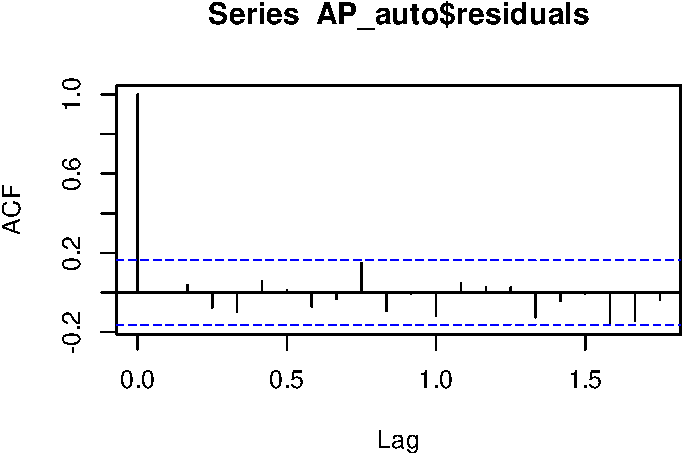
\includegraphics[keepaspectratio]{07-processi_continui_files/figure-pdf/unnamed-chunk-8-1.pdf}}

}

\caption{autocorrelazione empirica dei residui}

\end{figure}%

\begin{Shaded}
\begin{Highlighting}[]
\CommentTok{\# Osserviamo che nelle ascisse l\textquotesingle{}intervallo temporale (lag) è espresso in multipli del periodo di 12 mesi, per via della stagionalità della serie di partenza.}
\end{Highlighting}
\end{Shaded}

La funzione di autocorrelazione campionaria è uno strumento utile per
determinare eventuali stagionalità e il loro periodo \(k\), che si
ottiene in corrispondenza di ``picchi'' della funzione (più
precisamente, massimi locali). Bisogna tuttavia osservare che in
presenza di una componente lineare (detto anche \emph{trend}) della
serie storica, la funzone di autocorrelazione campionaria tende ad
essere uniformemente a valori grandi (e quindi maschera le
stagionalità).

\begin{Shaded}
\begin{Highlighting}[]
\FunctionTok{acf}\NormalTok{(AirPassengers)}
\end{Highlighting}
\end{Shaded}

\begin{figure}[H]

{\centering \pandocbounded{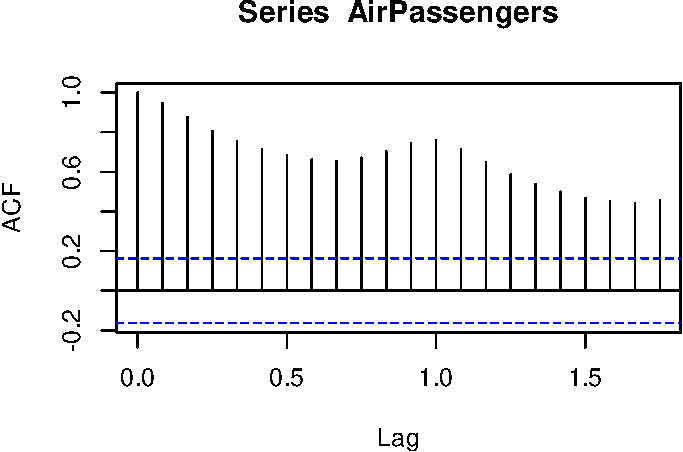
\includegraphics[keepaspectratio]{07-processi_continui_files/figure-pdf/unnamed-chunk-9-1.pdf}}

}

\caption{la funzione di autocorrelazione è uniformemente grande per via
del trend}

\end{figure}%

Un modo efficace per rimuovere questo effetto è passare ad una derivata
discreta della serie osservata, tramite la funzione \texttt{diff()}.

\begin{Shaded}
\begin{Highlighting}[]
\FunctionTok{acf}\NormalTok{(}\FunctionTok{diff}\NormalTok{(AirPassengers))}
\end{Highlighting}
\end{Shaded}

\begin{figure}[H]

{\centering \pandocbounded{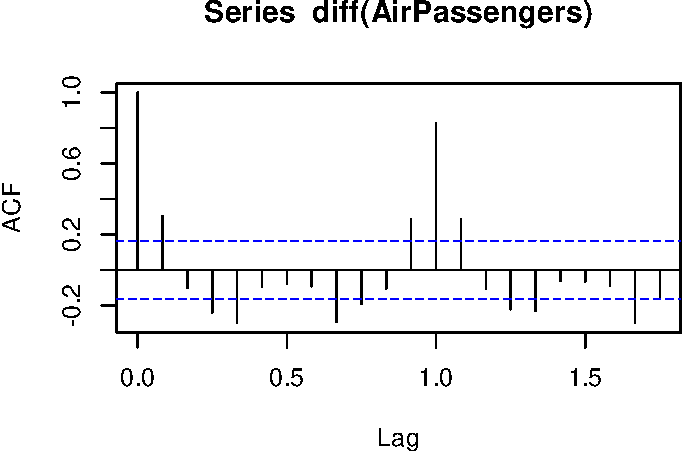
\includegraphics[keepaspectratio]{07-processi_continui_files/figure-pdf/unnamed-chunk-10-1.pdf}}

}

\caption{la derivata discreta rimuove il trend e la funzione di
autocorrelazione evidenzia la stagionalità a 12 mesi}

\end{figure}%

Oltre alla funzione di autocorrelazione campionaria, ci possiamo
chiedere cosa accada dei calcoli svolti passando alla trasformata di
Fourier, nel caso in cui l'ipotesi semplificativa \(C(k) = C(n-k)\) non
sia valida. Anche in questo caso, i passaggi sono approssimativamente
validi purché \(n\) diventi molto grande. In tal caso la stima che
abbiamo trovato
\[ \hat{C}(\xi) \approx \frac{ \abs{ \hat x(\xi)}^2}{n} = \frac{1} n \abs{ \sum_{t=0}^{n-1} x_t e^{-2\pi i t \xi /n}}^2\]
diventa esatta nel limite \(n \to \infty\) e passando al valor medio.
Precisamente, vale il seguente teorema.

Sia \((X_t)_{t =0}^\infty\) un processo a valori reali, stazionario in
senso lato, con media nulla \(\E{X_t} = 0\), e tale che
\[ \sum_{k=0}^\infty |C(k)| < \infty.\] Per ogni \(\xi \in [0,1]\), si
ponga
\[ \hat{C}(\xi) =  \sum_{k\in \mathbb{Z}} C(|k|)e^{-2\pi i k \xi}.\]
Allora vale il limite
\[ \lim_{ n \to \infty}   \frac{1} n \E{ \abs{ \sum_{t=0}^{n-1} X_t e^{-2\pi i t \xi }}^2} = \hat{C}(\xi).\]

In virtù della formula sopra, la trasformata di Fourier \(\hat{C}\)
della funzione di autocovarianza \(C\) è detta anche \emph{densità
spettrale di potenza} (in inglese \emph{power spectral density}), perché
rappresenta il valore medio (sia nel tempo che nel senso della
probabilità) dell'energia del processo associata alla frequenza \(\xi\).

Lo spettrogramma di una serie storica (ossia il modulo della trasformata
di Fourier, eventualmente in scala logaritmica) è uno strumento utile
per determinare eventuali periodicità. In R si può utilizzare
direttamente il comando \texttt{spectrum()}, che più precisamente
fonisce una stima della densità spettrale di potenza.

\begin{Shaded}
\begin{Highlighting}[]
\FunctionTok{spectrum}\NormalTok{(AirPassengers)}
\end{Highlighting}
\end{Shaded}

\begin{figure}[H]

{\centering \pandocbounded{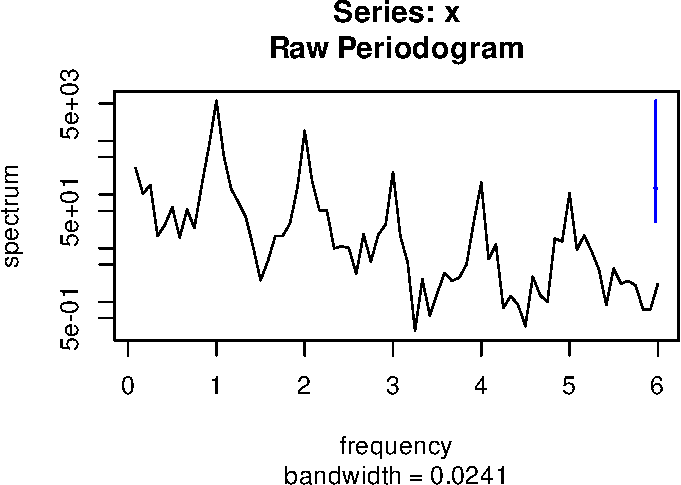
\includegraphics[keepaspectratio]{07-processi_continui_files/figure-pdf/unnamed-chunk-11-1.pdf}}

}

\caption{Stima della densità spettrale di potenza della serie
AirPassengers}

\end{figure}%

Lo spettro indica chiaramente la stagionalità (ricordiamo che è già
indicato che un periodo corrisponde a \(12\) mesi). Vediamo un esempio
diverso nel caso dei residui (che ricordiamo sono modellizzabili come un
rumore bianco gaussiano).

\begin{Shaded}
\begin{Highlighting}[]
\FunctionTok{spectrum}\NormalTok{(AP\_auto}\SpecialCharTok{$}\NormalTok{residuals)}
\end{Highlighting}
\end{Shaded}

\begin{figure}[H]

{\centering \pandocbounded{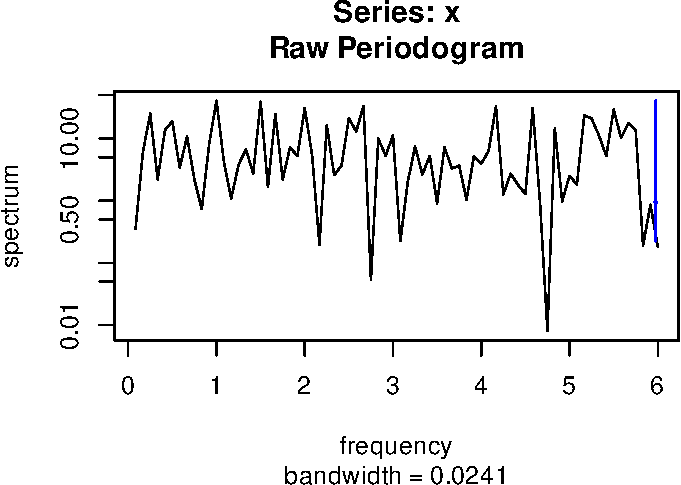
\includegraphics[keepaspectratio]{07-processi_continui_files/figure-pdf/unnamed-chunk-12-1.pdf}}

}

\caption{Stima della densità spettrale di potenza dei residui della
serie AirPassengers dopo un fit con un modello ARIMA}

\end{figure}%

In questo caso lo spettro non ha picchi particolari, segno in
particolare dell'assenza di stagionalità. Abbiamo anche calcolato che
nel caso di rumore bianco la densità spettrale di potenza (teorica) è
costante.

\bookmarksetup{startatroot}

\chapter{I teoremi limite}\label{sec-limite}

In questo capitolo accenniamo ad alcuni tra i principali teoremi limite
nella probabilità. Precisamente:

\begin{itemize}
\item
  Nella Sezione Sezione~\ref{sec-convergenze} definiamo le nozioni di
  convergenza per variabili aleatorie che useremo.
\item
  Nella Sezione Sezione~\ref{sec-lln} presentiamo la legge dei grandi
  numeri per variabili indipendenti, un risultato fondamentale che
  permette di collegare il concetto di frequenza delle osservazioni con
  la probabilità, nel caso di esperimenti indipendenti.
\item
  La Sezione Sezione~\ref{sec-ergodic} discute come estendere la legge
  dei grandi numeri al caso di processi più generali, ottenendo teoremi
  detti \emph{ergodici}.
\item
  Il teorema limite centrale è presentato nella Sezione
  Sezione~\ref{sec-clt} come naturale precisazione della legge dei
  grandi numeri.
\item
  Accenniamo brevemente alle applicazioni ai metodi Monte Carlo nella
  Sezione Sezione~\ref{sec-montecarlo}.
\item
  Infine discutiamo nella Sezione Sezione~\ref{sec-extreme} altri
  teoremi limite, ad esempio per il massimo o il minimo di variabili
  indpendenti.
\end{itemize}

\section{Convergenza di variabili aleatorie}\label{sec-convergenze}

Prima di discutere i teoremi limite di questa sezione, dobbiamo
specificare in che senso una successione di variabili aleatorie
\((X_n)_{n=1}^\infty\) approssimi una variabile aleatoria limite
\(X_\infty\) (o invertendo il punto di vista, la variabile limite
\(X_\infty\) sia una buona approssimazione delle variabili \(X_n\) al
crescere di \(n\)).

Ci sono molteplici nozioni, ma gli approcci principali sono
essentialmente due:

\begin{itemize}
\tightlist
\item
  si afferma che la distanza \(|X_n - X_\infty|\) diventa piccola, con
  grande probabilità, al crescere di \(n\),
\item
  oppure si afferma che le leggi di \(X_n\) convergono verso la legge di
  \(X_\infty\), ad esempio confrontandone le densità, le \(\CDF\), le
  \(\MGF\), i momenti, ecc.
\end{itemize}

La differenza più rilevante è che nel primo caso interviene la legge
congiunta delle variabili, ad esempio tra \(X_n\) e \(X_\infty\) per
costruire la variabile composta \(|X_n - X_\infty|\), mentre nel secondo
caso si considerano solamente le leggi marginali. Tipicamente il primo
approccio fornisce nozioni più forti di convergenza rispetto al secondo,
ma entrambi sono utili.

Partendo da queste premesse, diamo due definizioni legate al primo
approccio.

Siano \((X_n)_{n=1}^\infty\) e \(X_\infty\) variabili aleatorie a valori
in \(\R^d\). Diciamo che \(X_n\) converge verso \(X_\infty\)

\begin{itemize}
\tightlist
\item
  \emph{in probabilità} se per ogni \(\varepsilon>0\), si ha
  \[ \lim_{n \to \infty} P( |X_n - X_\infty| \le \varepsilon) = 1,\]
  oppure, equivalentemente,
  \[ \lim_{n \to \infty} P( |X_n - X_\infty| > \varepsilon) = 0;\]
\item
  \emph{in media quadratica} se vale
  \[ \lim_{n \to \infty } \E{ |X_n - X_\infty|^2} = 0.\]
\end{itemize}

In entrambi i casi vediamo che la legge congiunta di \((X_n, X_\infty)\)
è rilevante ai fini del calcolo delle probabilità o del valor medio.

\begin{remark}
C'è una implicazione tra le due nozioni di convergenza: se vale la
convergenza in media quadratica, allora vale anche in probabilità.
Questo perché la diseguaglianza di Markov implica che
\[ P( |X_n - X_\infty| > \varepsilon)  = P( |X_n - X_\infty|^2 > \varepsilon^2 ) \le \frac{ \E{ |X_n - X_\infty|^2}}{\varepsilon^2},\]
e quindi se il membro a destra è infinitesimo anche quello a sinistra lo
è (osserviamo che \(\varepsilon>0\) è arbritrario ma fissato, non
dipende da \(n\)).
\end{remark}

Mentre la nozione di convergenza in probabilità è abbastanza intuitiva
(si richiede che con probabilità che tende ad \(1\) le due variabili
\(X_n\) e \(X_\infty\) siano vicine meno di \(\varepsilon\)) il
vantaggio della convergenza in media quadratica è di poter sfruttare le
proprietà di calcolo legate al valor medio e alla varianza. Ad esempio,
vale il seguente risultato:

Siano \((X_n)_{n=1}^\infty\) variabili aleatorie a valori in \(\R^d\).
Allora \(X_n\) converge verso una costante \(c \in \R^d\) se e solo se
\[ \E{X_n} \to c \quad \text{e} \quad \Sigma_{X_n} \to 0.\]

\begin{proof}
Dimostriamolo per semplicità nel caso reale, ossia \(d=1\). Calcoliamo
\[ \begin{split} \E{ |X_n - c|^2 } & = \E{ |X_n - \E{X_n} + \E{X_n} - c|^2 } \\
& = \E{ |X_n - \E{X_n}|^2 } + \E{|\E{X_n} - c|^2 } \\
& \quad + 2 \E{ (X_n - \E{X_n})(\E{X_n} - c)}\\
& = \Var{X_n} + \E{|\E{X_n} - c|^2 }
\end{split}\] perché il doppio prodotto non contribuisce:
\[ \begin{split} \E{ (X_n - \E{X_n})(\E{X_n} - c)} &  = \E{ (X_n - \E{X_n})} (\E{X_n} - c) \\
& = (  \E{X_n} - \E{X_n}) (\E{X_n} - c) = 0.
\end{split}\] L'espressione trovata è la somma di due quantità positive,
è chiaro quindi che c'è convergenza in media quadratica verso una
costante \(c\) se e solo se entrambe convergono a zero.
\end{proof}

Veniamo ora ad una definizione di convergenza basata sul secondo
approccio. L'idea più semplice sarebbe di confrontare le densità delle
\(X_n\) con la densità del limite \(X_\infty\). Tuttavia tale nozione
sarebbe poco utile nel caso in cui ad esempio le \(X_n\) siano tutte
discrete mentre il limite è continuo. Questo ostacolo si può superare
confrontando invece le funzioni di ripartizione (nel caso di variabili
reali) oppure, nel caso vettoriale, confrontando le
\(\operatorname{MGF}\) o le funzioni caratteristiche.

Siano \((X_n)_{n=1}^\infty\) e \(X_\infty\) variabili aleatorie a valori
in \(\R^d\). Diciamo che \(X_n\) converge verso \(X_\infty\) \emph{in
legge} se

\begin{itemize}
\item
  nel caso \(d=1\), si ha
  \[ \lim_{n \to \infty} \CDF_{X_n}(t)  = \CDF_X(t)\] per ogni
  \(t \in \R\) eccetto al più i punti \(t\) in cui \(\CDF_X(t)\) ha una
  discontinuità di tipo salto (ossia \(P(X=t)>0\))
\item
  nel caso generale \(d \ge 1\), si ha
  \[  \lim_{n \to \infty} \MGF_{X_n}(t)  = \MGF_{X_\infty}(t)\] per ogni
  \(t\) in cui \(\MGF_{X_\infty}(t)\) sia finita, supponendo che
  \(\MGF_X(t)\) sia finita per \(t\) sufficientemente piccolo. In
  alternativa, si può richiedere la convergenza delle funzioni
  caratteristiche per ogni \(\omega \in \R\),
  \[ \lim_{n \to \infty} \varphi_{X_n}(\omega) =\varphi_{X_\infty}(\omega).\]
\end{itemize}

Se \(d=1\) e la variabile \(X_\infty\) ha densità continua, allora
\(\CDF_{X_\infty}\) è continua e possiamo richiedere la convergenza in
ogni \(t \in \R\). Tuttavia la convergenza in legge richiede comunque
meno della convergenza delle densità (anche supponendo che tutte le
\(X_n\) abbiano densità continua).

\begin{remark}
Il fatto che le due nozioni di convergenza in legge introdotto sopra
siano equivalenti se \(d=1\) è un risultato che non dimostriamo. Una
ulteriore riformulazione della convergenza in legge è la seguente: vale
\[ \lim_{n \to \infty} \E{ g(X_n)} = \E{g(X_\infty)}\] per ogni funzione
\(g\) continua ovunque e uniformemente limitata (ossia esiste una
costante \(c\) tale che \(|g(x)| \le c\) per ogni \(x \in \R^d\)).
\end{remark}

È possibile mostrare, ma non lo faremo, che la convergenza in
probabilità implica la convergenza in legge.

\section{Legge dei grandi numeri}\label{sec-lln}

La legge dei grandi numeri fornisce un supporto rigoroso
all'intepretazione di probabilità di una affermazione \(A\) come
\emph{frequenza relativa} con cui essa si realizza in una successione di
esperimenti ripetuti, sotto le stesse condizioni, ma tutti indipendenti
tra loro. In questa sezione ne diamo una dimostrazione usando la
convergenza in media quadratica (e quindi in probabilità). Prima di
affrontare il risultato generale, studiamo il caso più semplice delle
estrazioni con rimpiazzo dal solito modello dell'urna.

\subsection{Modello dell'urna}\label{modello-dellurna}

Supponiamo di avere un'urna in cui la frazione delle palline rosse è
\(r \in [0,1]\). Allora se si effettuano \(n\) estrazioni con rimpiazzo,
il numero \(R_n\) di palline rosse osservate ha densità binomiale di
parametri \((n,r)\). In particolare ha valor medio \(\E{R_n} = nr\) e
varianza \(\Var{R_n} = nr(1-r)\), ossia deviazione standard
\[\sigma_{R_n} = \sqrt{ n r (1-r)}.\] Ne segue che la frequenza relativa
di palline rosse osservate (sulle \(n\) estrazioni effettuate),
\(R_n/n\) ha valor medio \[ \E{ R_n/n} = r\] e varianza
\[  \Var{R_n/n}= \frac{n r(1-r)}{n^2} = \frac{r(1-r)}{n}.\] Passando
alla deviazione standard otteniamo per la frequenza relativa
\[ \sigma_{R_n/n} = \sqrt{ \frac{ r(1-r)}{n}}.\]

Informalmente, possiamo quindi scrivere la seguente approssimazione:
\[ \frac{R_n}{n} \approx r \pm \sqrt{ \frac{ r(1-r)}{n}}.\] Al tendere
di \(n \to \infty\) vediamo quindi che \(R_n/n\) converge verso la
frazione di palline rosse sul totale \(r\), che è anche la probabilità
di estrarre una pallina rossa in una singola estrazione. Precisamente,
al tendere di \(n \to \infty\), il valor medio di \(R_n/n\) è costante e
pari ad \(r\), mentre la varianza è infinitesima. Perciò, vale la
convergenza in media quadratica
\[ \E{ \abs{ \frac{R_n}{n} - r}^2   } = \frac{ r(1-r)}{n} \to 0 \] e
quindi in probabilità
\[ P\bra{ \abs{ \frac{R_n}{n} - r} \le \varepsilon} \ge 1- \frac{ r(1-r)}{n} \to 1 .\]

Questa è la versione della \emph{legge dei grandi numeri} nel modello
delle estrazioni dall'urna, che si estende ovviamente a una qualsiasi
situazione in cui vi siano un grande numero, potenzialmente illimitato,
di esperimenti ripetuti, tutti indipendenti tra loro, e ciascuno con
probabilità di sucesso \(p \in [0,1]\). La \emph{frequenza relativa del
numero di successi sul totale degli esperimenti} converge quindi alla
\emph{probabilità di successo di un singolo esperimento}.

Tale risulto permette l'intepretazione rigorosa di probabilità come
frequenza, un punto di vista piuttosto diffuso ma che comunque fin
dall'inizio abbiamo notato essere troppo restrittivo per molte
applicazioni -- in alcuni contesti non possiamo immaginare infiniti
esperimenti ripetuti.

La legge dei grandi numeri è comunque utile per la stima della
probabilità \(p\) di successo in un esperimento, qualora non fosse nota.
Tornando all'esempio dell'urna e riprendendo l'esempio del robot,
supponiamo infatti che inizialmente non sia informato della frazione di
palline rosse in essa contenuta e quindi introduca una variabile
aleatoria \(R\) a valori in \([0,1]\) (ad esempio a priori uniforme, ma
una qualsiasi densità andrebbe bene lo stesso). Allora, può affermare
che
\[ \begin{split} P( |R_n/n - R| \le \varepsilon ) & = \int_0^1 P( |R_n/n - r| \le \varepsilon |R = r) dr \\
&  \ge 1- \frac{\int_0^1 r(1-r) dr }{n\varepsilon^2} = 1-  \frac{1}{6n \varepsilon^2}  \to 1
\end{split}\] per \(n \to \infty\), ossia con alta probabilità la
frequenza relativa \(R_n/n\) è vicina alla variabile \(R\) (precisamente
abbiamo mostrato la convergenza in probabilità). Notiamo che la
probabilità calcolata sopra è rispetto all'informazione a priori, ossia
prima di effettuare le estrazioni (o prima di essere informati
dell'esito).

\begin{remark}
Nonostante l'apparente semplicità, la legge dei grandi numeri nel caso
delle estrazioni dall'urna, o più in generale in situazioni di
esperimenti indipendenti ripetuti con esito binario
(successo/insuccesso) ha molteplici applicazioni. Usando questo
risultato possiamo spiegare perché l'istogramma relativo ad \(n\)
osservazioni di variabili indipendenti, tutte con la stessa densità
debba essere molto vicino al grafico della densità teorica. Abbiamo
visto l'utilità di questo fatto nella sezione Sezione~\ref{sec-test} per
valutare l'ipotesi di gaussianità, ad esempio dei residui di una
regressione.

Siano infatti \((X_i)_{i=1}^n\) variabili indipendenti tutte con la
medesima densità (ad esempio continua). Allora supponendo di considerare
un rettangolo di base \(a<b \in \R\), l'istogramma delle frequenze
(assolute) avrà altezza \(H(a,b)\) pari al numero delle \(X_i\) tali che
\(a<X_i \le b\), mentre quello delle densità è ulteriormente diviso il
numero delle osservazioni \(n\) e per la lunghezza della base \((b-a)\).
Questa differenza è particolarmente rilevante se i rettangoli non hanno
tutti la stessa lunghezza della base, mentre nel caso di basi con la
stessa lunghezza è solamente una dilatazione nell'asse delle ordinate.

\begin{Shaded}
\begin{Highlighting}[]
\CommentTok{\# usiamo i dati del dataset Iris}

\FunctionTok{par}\NormalTok{(}\AttributeTok{mfrow=}\FunctionTok{c}\NormalTok{(}\DecValTok{1}\NormalTok{,}\DecValTok{2}\NormalTok{))}

\FunctionTok{hist}\NormalTok{(iris}\SpecialCharTok{$}\NormalTok{Sepal.Length, }\AttributeTok{freq=}\ConstantTok{TRUE}\NormalTok{, }\AttributeTok{col=}\NormalTok{miei\_colori[}\DecValTok{1}\NormalTok{], }\AttributeTok{main=}\StringTok{""}\NormalTok{, }\AttributeTok{xlab=}\StringTok{"lunghezza sepali"}\NormalTok{, }\AttributeTok{ylab=}\StringTok{"frequenza"}\NormalTok{)}

\FunctionTok{hist}\NormalTok{(iris}\SpecialCharTok{$}\NormalTok{Sepal.Length, }\AttributeTok{freq=}\ConstantTok{FALSE}\NormalTok{, }\AttributeTok{col=}\NormalTok{miei\_colori[}\DecValTok{2}\NormalTok{], }\AttributeTok{main=}\StringTok{""}\NormalTok{, }\AttributeTok{xlab=}\StringTok{"lunghezza sepali"}\NormalTok{, }\AttributeTok{ylab=}\StringTok{"densità"}\NormalTok{)}
\end{Highlighting}
\end{Shaded}

\begin{figure}[H]

{\centering \pandocbounded{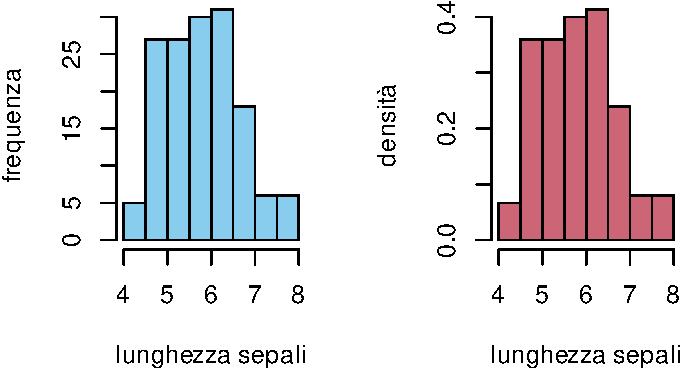
\includegraphics[keepaspectratio]{08-teoremi_limite_files/figure-pdf/unnamed-chunk-2-1.pdf}}

}

\caption{confronto tra istogramma delle frequenze (a sinistra) e delle
densità (a destra)}

\end{figure}%

Possiamo quindi pensare ad un ``successo'' se \(X_i \in (a,b]\), con
probabilità
\[ r = P(X_1 \in (a,b]) = \int_a^b p(X_1 = x) dx\approx p(X_1=a)(b-a),\]
dove nell'ultima approssimazione supponiamo la densità abbastanza
regolare e \(b-a\) sufficientemente piccolo.

Considerando \(n\) esperimenti indipendenti si avrà quindi che
\[ \frac{ H(a,b)}{n} \approx r  \pm \sqrt{ \frac{ r(1-r)}{n}} \approx p(X_1=a)(b-a),\]
e quindi l'istogramma delle densità, che ha altezza \(H(a,b)/(n(b-a))\),
è, con alta probabilità vicino alla densità comune. Un ragionamento
simile si può effettuare anche per variabili discrete, e pure per le
funzioni di ripartizione e i quantili (giustificando anche l'approccio
qualitativo all'ipotesi di gaussianità mediante QQ-plot).
\end{remark}

\subsection{Un risultato generale}\label{un-risultato-generale}

Il risultato valido per la frequenza relativa dei successi in \(n\)
esperimenti indipendenti si può estendere a situazioni più generali, in
cui l'esito di ciascun ``esperimento'' sia una variabile aleatoria
\(X_i\) a valori reali (in realtà anche vettoriali, ma non ce ne
occupiamo per semplicità). Immaginiamo la situazione in cui si
effettuano più misurazioni di una medesima quantità, affette da errori,
se presenti, indipendenti o comunque poco correlati tra loro (dovuti ad
esempio a circostanze esterne che non possiamo controllare). Allora la
frequenza relativa dei successi può essere sostituita dalla media
empirica \[ \bar{X}_n = \frac 1 n \sum_{i=1}^n X_i,\] che è una
variabile aleatoria (come abbiamo già osservato nella sezione precedente
la legge dei grandi numeri è un risultato di convergenza rispetto
all'informazione a priori, ossia prima di essere informati degli esiti
degli esperimenti, quindi \(\bar{X}_n\) non è nota).

Nel caso degli esperimenti, per dedurre la convergenza in media
quadratica delle frequenze relative, abbiamo usato il fatto che la legge
della somma \(\sum_{i=1}^nX_i\), ossia il numero di successi, ha densità
discreta binomiale di parametri \((n,p)\). Tuttavia ripercorrendo
l'argomento, basta conoscere molto meno: infatti è sufficiente che il
valor medio \(\E{\bar{X}_n}\) converga a una costante \(m\) e la
varianza \(\Var{\bar{X}_n}\) sia infinitesima per \(n \to \infty\):
sotto queste condizioni infatti il criterio della Sezione
Sezione~\ref{sec-convergenze} garantisce la convergenza
\(\lim_{n \to \infty} \bar{X}_n = m\).

Sfruttando questa osservazione, enunciamo il seguente risultato, noto
appunto come legge dei grandi numeri\footnote{più precisamente è detto
  legge \emph{debole} dei grandi numeri}. Notiamo che l'indipendenza può
essere indebolita richiedendo solo l'assenza di correlazione.

Siano \((X_n)_{n =1}^\infty\) variabili aleatorie non correlate, tutte
con lo stesso valor medio e varianza
\[ \E{X_n} = m, \quad \Var{X_n} = \sigma^2 < \infty.\] Allora, si ha la
convergenza in media quadratica (e quindi in probabilità)
\[ \lim_{n \to \infty} \frac{1}{n} \sum_{i=1}^n X_i = m.\]

\begin{proof}
Posta \(\bar{X}_n = \frac 1 n \sum_{i=1}^n X_i\) la media campionaria,
usiamo la linearità per calcolare\\
\[\begin{split} \E{\bar{X}_n } & = \E{ \frac  1 n \sum_{i=1}^n X_i}   = \frac 1 n \sum_{i=1}^n \E{X_i} = \frac 1 n \sum_{i=1}^n m \\
& = m \end{split}\] e l'ipotesi \(\Cov{X_i, X_j} = 0\) per \(i \neq j\)
per ottenere che
\[\begin{split} \Var{\bar{X}_n } & = \frac 1 {n^2}  \Var{\sum_{i=1}^n X_i}\\
& = \frac 1 {n^2} \sum_{i=1}^n \Var{X_i} \\
& = \frac 1{n^2 } \sum_{i=1}^n \sigma^2 \\
& = \frac{1}{n^2} \cdot  n \sigma^2 \\
& = \frac{\sigma^2}{n},
\end{split}\] che al tendere di \(n \to \infty\) è infinitesima.
\end{proof}

\begin{remark}
Dalla dimostrazione segue che la deviazione standard della variabile
\(\bar{X}_n\) è
\[\sigma_{\bar{X}_n} = \sqrt{ \Var{ \bar{X}_n}} = \frac{\sigma}{\sqrt{n}},\]
e quindi informalmente possiamo scrivere
\[ \bar{X}_n = m \pm  \frac{\sigma}{\sqrt{n}}.\]
\end{remark}

La legge dei grandi numeri è un risultato generale, che può essere
applicato in molteplici situazioni. Ad esempio, ricordando la
definizione di varianza campionaria
\[ \bar{\sigma}^2_n = \frac{1}{n} \sum_{i=1}^n (X_i - \bar{X}_n)^2,\] è
possibile usare la legge dei grandi numeri per dedurre la convergenza in
media quadratica e in probabilità di
\[ \lim_{n \to \infty} \bar{\sigma}^2_n = \sigma^2,\] supponendo ad
esempio che le \((X_i)_i\) siano tutte indipendenti, tutte con le stessa
legge e dotate di momento quarto finito, quindi in particolare i momenti
sono tutti uguali: \[ m_1 = \E{X_i}, \quad m_2 = \E{X_i^2}.\] Infatti,
basta riscrivere la varianza campionaria nel modo alternativo
\[ \bar \sigma_n^2 = \frac 1 n \sum_{i=1}^n X_i^2 - (\bar{X_n})^2 = \overline{ (X^2)}_n - (\bar{X_n})^2,\]
e notare che sotto l'ipotesi di momento quarto finito e indipendenza,
non solo \[\lim_{n \to \infty }\bar{X_n} = m_1,\] ma anche
\[ \lim_{n \to \infty} \overline{ (X^2)}_n = m_2.\] Di conseguenza,
usando la definizione di convergenza, si può argomentare che
\[ \lim_{n \to \infty }\bar\sigma_n^2 = \lim_{n \to \infty} \sqa{ \overline{ (X^2)}_n - (\bar{X_n})^2} = m_2 - m_1^2 = \sigma^2.\]

\section{Teoremi Ergodici}\label{sec-ergodic}

L'argomento che ha portato alla dimostrazione della legge dei grandi
numeri nella sezione precedente usa fortemente l'ipotesi di non
correlazione tra le variabili \((X_i)_{i=1}^\infty\). Senza questa
ipotesi, la varianza della media campionaria è in generale la somma di
\(n^2\) termini
\[ \Var{ \bar {X}_n} = \frac{1}{n^2} \sum_{i,j=1}^n\Cov{X_i, X_j},\] e
quindi non segue necessariamente che sia infinitesima, anche tenendo in
conto del denominatore \(n^2\). Questo tuttavia può accadere se
\(\Cov{X_i, X_j}\) è infinitesimo per ``molte'' coppie, come avviene
spesso nel caso di processi stocastici.

Dato infatti un processo stocastico \((X_t)_{t = 1}^\infty\), ad esempio
sull'insieme dei tempi \(\mathcal{T} = \cur{1,2,3\ldots}\), la media
\(\bar{X}_T = \frac 1 T \sum_{t=1}^T X_t\) si può pensare come alla
media della traiettoria del processo sui primi \(T\) tempi. Più in
generale, se l'insieme degli stati \(E\) del processo non è un
sottoinsieme di \(\R\), si può considerare una qualsiasi funzione
\(g:E \to \R\) e considerare la media
\[ \overline{ g(X)}_T = \frac 1 T \sum_{t=1}^T g(X_t).\] La funzione
\(g\) è anche detta anche \emph{osservabile} e rappresenta una quantità
misurabile a partire dal processo. La legge dei grandi numeri in questo
caso riguarda la convergenza al tendere dei tempi all'infinito delle
variabili aleatorie \(\overline{ g(X)}_T\),
\[ \lim_{T \to \infty }\overline{ g(X)}_T. \] Se si suppone che il
processo \((X_t)_t\) sia stazionario, è possibile identificare il limite
(se esiste) come il valor medio di \(g\) rispetto alla legge marginale
in un qualsiasi istante, ad esempio nel caso di \(E\) discreto
\[ \E{g(X_i)} = \sum_{ x \in E} g(x) P(X_i=x).\]

Consideriamo come osservabile \(g\) la funzione indicatrice di un
qualsiasi stato \(x_0 \in E\),
\[ g(x) = \begin{cases} 1 & \text{se $x = x_0$}\\
0 & \text{se $x \neq x_0$.}\end{cases}\] Allora \(\overline{g(X)}_T\) è
la frazione di tempo trascorsa dal processo sullo stato \(x_0\), dal
tempo \(t=1\) al tempo \(t=T\). Il valor medio invece è semplicemente la
probabilità \(\E{g(X_i)} = P(X_i = x_0)\). La stessa cosa avviene se
invece dell'indicatrice di uno stato, si considera l'indicatrice di un
sottoinsieme \(E_0 \subseteq E\) di stati.

La possibilità di identificare le due medie, quella sui tempi
\(\overline{g(X)}_T\) e quella sugli stati \(\E{g(X_i)}\) è in un certo
senso analoga all'intepretazione della probabilità come limite delle
frequenze sugli esperimenti ripetuti. Risultati che garantiscono tale
possibilità sono storicamente detti \emph{teoremi ergodici}, un termine
che proviene dalla meccanica statistica.

Con una opportuna variante dell'argomento per la legge dei grandi
numeri, possiamo mostrare il seguente risultato.

Sia \((X_t)_{t =0}^\infty\) un processo stazionario sull'insieme degli
stati \(E\) e sia \(g: E \to \R\) una osservabile. Se
\[ \lim_{t \to \infty} \Cov{g(X_0), g(X_t)} = 0,\] allora vale la
convergenza in media quadratica e in probabilità
\[ \lim_{ T \to \infty} \overline{g(X)}_T = \E{ g(X_0)}.\] (dove per
semplicità abbiamo specificato \(X_0\), ma un qualsiasi altro tempo
\(X_t\) sarebbe lo stesso, essendo il processo stazionario).

\begin{proof}
Poniamo per semplicità di notazione \(Y_t = g(X_t)\). L'ipotesi di
stazionarietà di \((X_t)\) implica che anche \((Y_t)\) sia stazionario e
quindi la sua funzione di autocovarianza soddisfa
\[ C(s,t) =  C(0, |t-s|) = \Cov{g(X_0), g(X_{|t-s|})},\] che per ipotesi
è infinitesima al tendere di \(|t-s| \to \infty\). Consideriamo ora il
valor medio e la varianza della variabile aleatoria
\[\bar{Y}_T = \frac 1 T \sum_{t=1}^TY_t.\] Per linearità del valor medio
e stazionarietà
\[ \E{ \bar{Y}_T} = \frac 1 T \sum_{t=1}^T \E{Y_t} = \E{Y_0} = \E{g(X_0)}\]
è costante, mentre per la varianza scriviamo
\[\Var{\bar{Y}_T } = \frac 1 {T^2} \sum_{s,t=1}^T C(s,t) = \frac 1 {T^2} \sum_{s,t=1}^T C(0,|t-s|) .\]
Osserviamo che, per ciascun \(k=0, \ldots, T\), vi sono al più \(2T\)
coppie \((s,t)\) nella somma sopra con \(|t-s| = k\) (corrispondenti al
casi \(t=s+k\) e \(t=s-k\)). Pertanto possiamo stimare
\[ \frac 1 {T^2} \sum_{s,t=1}^T C(0,|t-s|) \le \frac{1}{T^2} \sum_{k=0}^T 2 T |C(0,k)| \le \frac{2}{T} \sum_{k=0}^T  |C(0,k)|.\]
Il fatto che la somma sopra sia infinitesima, grazie all'ipotesi che
\(C(0,k)\) lo sia, è una conseguenza nota di un teorema di analisi
dovuto a Cesaro. Ecco i dettagli: fissato \(\varepsilon>0\), sia
\(k_{\varepsilon}\) tale che, \[
\text{ se $k> k_{\varepsilon}$, allora $|C(0,k)| < \varepsilon$.}
\] Ne segue che
\[ \frac{2}{T} \sum_{k=0}^T  |C(0,k)| \le \frac{2}{T} \sum_{k=0}^{k_\varepsilon} |C(0,k)| + \frac{2}{T} |T-k_{\varepsilon}| \varepsilon\]
e il membro di destra al tendere di \(T \to \infty\) è più piccolo di
\(2 \varepsilon\). Essendo \(\varepsilon\) arbitrariamente piccolo,
concludiamo che
\[\lim_{ T \to \infty} \frac{2}{T} \sum_{k=0}^T  |C(0,k)| = 0.\]
\end{proof}

\begin{remark}
Con un argomento simile si può ottenere un teorema ergodico anche nel
caso di processi a tempi continui (con applicazioni ad esempio ai
processi di Markov a salti). In tal caso la media sui tempi va intesa
come l'integrale \[ \overline{g(X)}_T = \frac 1 T \int_0^T g(X_t) dt.\]
\end{remark}

Per applicare il teorema è quindi importante verificare, oltre alla
stazionarietà del processo, l'ipotesi sul limite della funzione di
autocovarianza (detta anche appunto ipotesi di ergodicità). In molti
modelli è possibile argomentare in generale che essa vale. Diamo i
seguenti risultati senza vederne la dimostrazione.

Sia \((X_t)_{t}\) una catena di Markov stazionaria e irriducibile su un
insieme di stati finito \(E\). Allora per ogni \(g: E  \to \R\) vale la
convergenza
\[ \lim_{ T \to \infty} \overline{g(X)}_T =  \sum_{i \in E} g(i) \pi_i,\]
dove \(\pi = (\pi_i)_{i\in E}\) è l'unica distribuzione invariante per
la catena.

In particolare, la frazione di tempo trascorsa dalla catena su uno stato
è, nel limite, pari alla probabilità che la catena si trovi su quello
stato.

Un teorema analogo vale per processi di Markov a salti, dove la media
nel tempo è intesa come integrale. Vediamo infine il caso dei processi a
stati continui. In questo caso siamo interessati alla convergenza delle
medie e delle funzioni di autocovarianza campionarie.

Sia \((X_t)_{t}\) un processo \(\operatorname{ARIMA}(p,0,q)\)
stazionario. Allora \[ \lim_{T \to \infty} \overline{X}_T = 0,\] e per
ogni \(t\in \mathbb{N}\),
\[ \lim_{T \to \infty} \frac 1 T \sum_{s=1}^T X_s X_{s+t} = C(0,t).\]

L'ultimo limite sopra mostra che la funzione di autocovarianza empirica
converge a quella teorica: questo teorema, che pure vale per processi
stazionari anche più generali degli ARIMA, giustifica ulteriormente
l'uso della funzione di autocorrelazione empirica (tramite ad esempio la
funzione \texttt{acf()} in \(R\)) per stimare quella teorica.

\section{Il teorema limite centrale}\label{sec-clt}

Il teorema limite centrale è un raffinamento della legge dei grandi
numeri, in cui si rende più precisa la convergenza delle medie
empiriche, mostrando che le oscillazioni sono approssimabili tramite
variabili gaussiane, qualsiasi fosse la distribuzione delle variabili di
partenza. Questo risultato di ``universalità'' delle densità gaussiane
fornisce quindi una ulteriore giustificazione della loro applicazione
così diffusa in molteplici ambiti.

\subsection{Il modello dell'urna}\label{il-modello-dellurna}

Torniamo all'esempio delle estrazioni con rimpiazzo da un'urna
contenente una frazione \(r \in (0,1)\) di palline rosse. Posto \(R_n\)
il numero di palline rosse estratte, la legge dei grandi numeri afferma
(in versione informale) che vale l'approssimazione
\[ \frac{R_n}{n} \approx r \pm \sqrt{ \frac{ r(1-r) }{n}}.\] Il teorema
limite centrale rende più preciso il simbolo \(\pm\), mostrando che per
una variabile gaussiana \(Z\) standard, ossia \(\mathcal{N}(0,1)\), vale
\[ \frac{R_n}{n} \approx r + Z \sqrt{ \frac{ r(1-r) }{n}},\] dove
l'approssimazione è nel senso della convergenza in legge.
Equivalentemente, la variabile binomiale \(R_n\) si approssima quindi
con una variabile gaussiana avente la stessa media \(nr\) e varianza
\(n r(1-r)\). Possiamo visualizzare questo risultato graficamente
confrontando la densità discreta binomiale e la gaussiana
corrispondente.

\begin{Shaded}
\begin{Highlighting}[]
\NormalTok{n}\OtherTok{=}\DecValTok{50}
\NormalTok{r}\OtherTok{=}\DecValTok{1}\SpecialCharTok{/}\DecValTok{3}
\NormalTok{k}\OtherTok{=}\DecValTok{0}\SpecialCharTok{:}\NormalTok{n}

\FunctionTok{par}\NormalTok{(}\AttributeTok{mfrow=}\FunctionTok{c}\NormalTok{(}\DecValTok{1}\NormalTok{,}\DecValTok{2}\NormalTok{))}

\FunctionTok{plot}\NormalTok{(k, }\FunctionTok{dbinom}\NormalTok{(k, n, r), }\AttributeTok{type=}\StringTok{\textquotesingle{}s\textquotesingle{}}\NormalTok{, }\AttributeTok{lwd=}\DecValTok{3}\NormalTok{, }\AttributeTok{col=}\NormalTok{miei\_colori[}\DecValTok{4}\NormalTok{], }\AttributeTok{ylab=}\StringTok{\textquotesingle{}probabilità\textquotesingle{}}\NormalTok{, }\AttributeTok{main=}\StringTok{\textquotesingle{}densità binomiale\textquotesingle{}}\NormalTok{)}

\FunctionTok{plot}\NormalTok{(k, }\FunctionTok{dnorm}\NormalTok{(k, }\AttributeTok{mean=}\NormalTok{r}\SpecialCharTok{*}\NormalTok{n, }\AttributeTok{sd=}\FunctionTok{sqrt}\NormalTok{(r}\SpecialCharTok{*}\NormalTok{(}\DecValTok{1}\SpecialCharTok{{-}}\NormalTok{r)}\SpecialCharTok{*}\NormalTok{n)), }\AttributeTok{type=}\StringTok{\textquotesingle{}l\textquotesingle{}}\NormalTok{, }\AttributeTok{lwd=}\DecValTok{3}\NormalTok{, }\AttributeTok{ylab=}\StringTok{\textquotesingle{}densità\textquotesingle{}}\NormalTok{, }\AttributeTok{col=}\NormalTok{miei\_colori[}\DecValTok{2}\NormalTok{], }\AttributeTok{main=}\StringTok{\textquotesingle{}densità gaussiana\textquotesingle{}}\NormalTok{)}
\end{Highlighting}
\end{Shaded}

\begin{figure}[H]

{\centering \pandocbounded{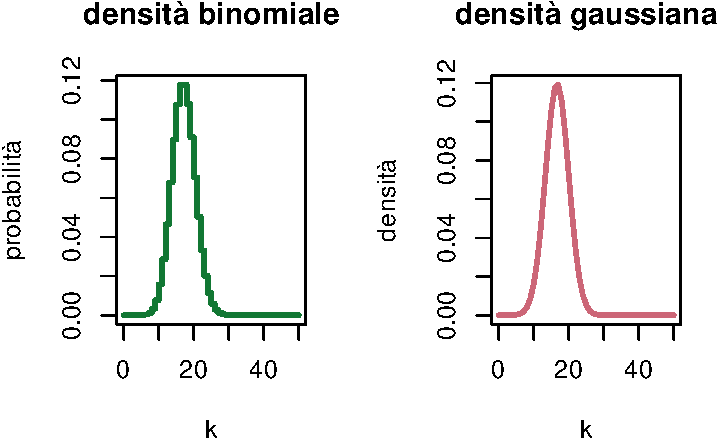
\includegraphics[keepaspectratio]{08-teoremi_limite_files/figure-pdf/unnamed-chunk-3-1.pdf}}

}

\caption{confronto tra densità binomiale di parametri \(n=50\),
\(r=1/3\) e la densità gaussiana con medesima media \(nr\) e varianza
\(nr(1-r)\).}

\end{figure}%

L'approssimazione vale nel senso della convergenza in legge (quindi si
confrontano le \(\CDF\) piuttosto che le densità). Per ogni intervallo
\([a,b]\subseteq \R\) (anche con \(a = -\infty\) oppure \(b = \infty\)),
si ha che
\[ \lim_{n \to \infty} P\bra{  a \sqrt{ \frac{ r(1-r) }{n}} \le  \frac{R_n}{n } -r \le  b\sqrt{ \frac{ r(1-r) }{n}}  }  =  \int_a^b \exp\bra{-\frac{ z^2}{2} } \frac{dz}{\sqrt{ 2 \pi}}.\]

Per trattare meglio la convergenza conviene introdurre le variabili
standardizzate delle \(R_n/n\), ossia
\[Z_n = \bra{ \frac{R_n}{n}-r} \sqrt{ \frac{n }{r(1-r)}},\] in modo che
la convergenza in legge sia \(\lim_{n \to \infty} Z_n = Z\), ossia
\[ \CDF_{Z_n}(t) \to \CDF_Z(t)\] per ogni \(t \in \R\). Possiamo
verificare numericamente la validità di questa approssimazione scrivendo
\(\CDF_{Z_n}\) in termini della \(\CDF_{R_n}\), che è binomiale. Usando
l'identità \[ \CDF_{aX+b}(t) = \CDF_X((t-b)/a)\] valida per \(a>0\),
\(b\in \R\), possiamo scrivere
\[ \CDF_{Z_n}(t) = \CDF_{R_n}\bra{ n r + t \sqrt{nr(1-r)} },\] e
visualizzare graficamente tramite opportuni comandi R.

\begin{Shaded}
\begin{Highlighting}[]
\NormalTok{r}\OtherTok{=}\DecValTok{1}\SpecialCharTok{/}\DecValTok{2}
\NormalTok{t }\OtherTok{=} \FunctionTok{seq}\NormalTok{(}\SpecialCharTok{{-}}\DecValTok{3}\NormalTok{, }\DecValTok{3}\NormalTok{, }\AttributeTok{by=}\FloatTok{0.001}\NormalTok{)}


\FunctionTok{par}\NormalTok{(}\AttributeTok{mfrow=}\FunctionTok{c}\NormalTok{(}\DecValTok{1}\NormalTok{,}\DecValTok{3}\NormalTok{))}

\FunctionTok{plot}\NormalTok{(t, }\FunctionTok{pnorm}\NormalTok{(t), }\AttributeTok{type=}\StringTok{\textquotesingle{}l\textquotesingle{}}\NormalTok{, }\AttributeTok{lwd=}\DecValTok{2}\NormalTok{, }\AttributeTok{col=}\NormalTok{miei\_colori[}\DecValTok{2}\NormalTok{], }\AttributeTok{xlab=}\StringTok{\textquotesingle{}t\textquotesingle{}}\NormalTok{, }\AttributeTok{ylab=}\StringTok{\textquotesingle{}CDF\textquotesingle{}}\NormalTok{, }\AttributeTok{main=}\StringTok{"n=10"}\NormalTok{)}

\NormalTok{n}\OtherTok{=}\DecValTok{10}
\FunctionTok{lines}\NormalTok{(t, }\FunctionTok{pbinom}\NormalTok{( n}\SpecialCharTok{*}\NormalTok{r }\SpecialCharTok{+}\NormalTok{ t }\SpecialCharTok{*}\FunctionTok{sqrt}\NormalTok{(n }\SpecialCharTok{*}\NormalTok{ r }\SpecialCharTok{*}\NormalTok{(}\DecValTok{1}\SpecialCharTok{{-}}\NormalTok{r)) , n, r),}\AttributeTok{lwd=}\DecValTok{2}\NormalTok{, }\AttributeTok{col=}\NormalTok{miei\_colori[}\DecValTok{4}\NormalTok{])}

\FunctionTok{plot}\NormalTok{(t, }\FunctionTok{pnorm}\NormalTok{(t), }\AttributeTok{type=}\StringTok{\textquotesingle{}l\textquotesingle{}}\NormalTok{, }\AttributeTok{lwd=}\DecValTok{2}\NormalTok{, }\AttributeTok{col=}\NormalTok{miei\_colori[}\DecValTok{2}\NormalTok{], }\AttributeTok{xlab=}\StringTok{\textquotesingle{}t\textquotesingle{}}\NormalTok{, }\AttributeTok{ylab=}\StringTok{\textquotesingle{}\textquotesingle{}}\NormalTok{, }\AttributeTok{main=}\StringTok{\textquotesingle{}n=50\textquotesingle{}}\NormalTok{)}

\NormalTok{n}\OtherTok{=}\DecValTok{50}
\FunctionTok{lines}\NormalTok{(t, }\FunctionTok{pbinom}\NormalTok{( n}\SpecialCharTok{*}\NormalTok{r }\SpecialCharTok{+}\NormalTok{ t }\SpecialCharTok{*}\FunctionTok{sqrt}\NormalTok{(n }\SpecialCharTok{*}\NormalTok{ r }\SpecialCharTok{*}\NormalTok{(}\DecValTok{1}\SpecialCharTok{{-}}\NormalTok{r)) , n, r),}\AttributeTok{lwd=}\DecValTok{2}\NormalTok{, }\AttributeTok{col=}\NormalTok{miei\_colori[}\DecValTok{4}\NormalTok{])}

\FunctionTok{plot}\NormalTok{(t, }\FunctionTok{pnorm}\NormalTok{(t), }\AttributeTok{type=}\StringTok{\textquotesingle{}l\textquotesingle{}}\NormalTok{, }\AttributeTok{lwd=}\DecValTok{2}\NormalTok{, }\AttributeTok{col=}\NormalTok{miei\_colori[}\DecValTok{2}\NormalTok{], }\AttributeTok{xlab=}\StringTok{\textquotesingle{}t\textquotesingle{}}\NormalTok{,}\AttributeTok{ylab=}\StringTok{\textquotesingle{}\textquotesingle{}}\NormalTok{, }\AttributeTok{main=}\StringTok{\textquotesingle{}n=100\textquotesingle{}}\NormalTok{)}
\NormalTok{n}\OtherTok{=}\DecValTok{100}
\FunctionTok{lines}\NormalTok{(t, }\FunctionTok{pbinom}\NormalTok{( n}\SpecialCharTok{*}\NormalTok{r }\SpecialCharTok{+}\NormalTok{ t }\SpecialCharTok{*}\FunctionTok{sqrt}\NormalTok{(n }\SpecialCharTok{*}\NormalTok{ r }\SpecialCharTok{*}\NormalTok{(}\DecValTok{1}\SpecialCharTok{{-}}\NormalTok{r)) , n, r),}\AttributeTok{lwd=}\DecValTok{2}\NormalTok{, }\AttributeTok{col=}\NormalTok{miei\_colori[}\DecValTok{4}\NormalTok{])}
\end{Highlighting}
\end{Shaded}

\begin{figure}[H]

{\centering \pandocbounded{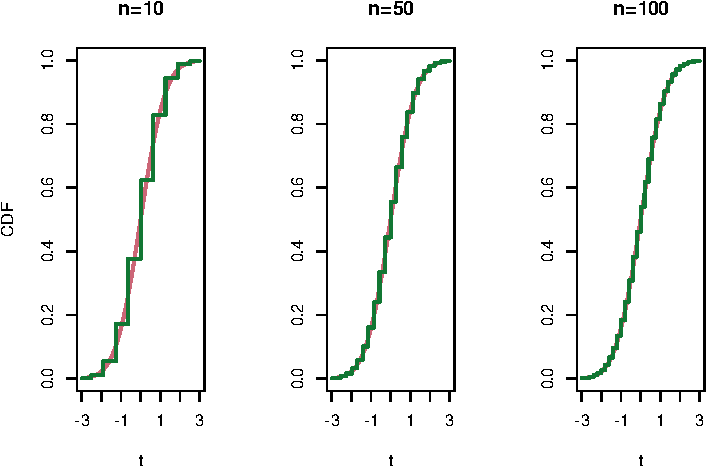
\includegraphics[keepaspectratio]{08-teoremi_limite_files/figure-pdf/unnamed-chunk-4-1.pdf}}

}

\caption{confronto tra le \(\CDF_{Z_n}\) e \(\CDF_Z\) al crescere di
\(n\).}

\end{figure}%

\subsection{Il caso generale}\label{il-caso-generale}

Nonostante l'evidente validità dell'approssimazione, la dimostrazione
della convergenza richiederebbe qualche calcolo non del tutto immediato
già nel caso delle estrazioni dall'urna. Perciò affrontiamo direttamente
una dimostrazione del risultato generale per l'approssimazione gaussiana
delle medie campionarie di variabili indipendenti. Tale teorema è noto
come \emph{teorema limite centrale}, dove l'aggettivo ``centrale'' si
riferisce all'importanza (appunto, centrale) tra i teoremi limite nella
teoria della probabilità (in particolare, non ha a che fare con il fatto
che le variabili siano centrate perché standardizzate).

Ricordiamo che informalmente, la legge dei grandi numeri si scriveva
come l'approssimazione
\[ \bar{X}_n \approx m \pm \frac{\sigma}{\sqrt{n}}.\] Come nel caso
delle estrazioni dall'urna, possiamo rendere più preciso il simbolo
\(\pm\) introducendo una variabile gaussiana \(Z\) standard
\(\mathcal{N}(0,1)\).

Siano \((X_n)_{n=1}^\infty\) variabili aleatorie reali indipendenti,
tutte con la stessa legge e quindi valor medio \[ m = \E{X_n}\] e
varianza \[\sigma^2 = \Var{X_n} \in (0, \infty)\] (che supponiamo
finita). Allora, posta \(\bar{X}_n = \frac{1}{n} \sum_{i=1}^n X_i\) la
media campionaria e \[Z_n = (\bar{X}_n  -m ) \frac{ \sqrt{ n}}{\sigma}\]
la sua standardizzata, si ha la convergenza in legge
\[ \lim_{n \to \infty }Z_n = Z,\] dove \(Z\) è gaussiana standard.
Esplicitamente, per ogni \([a,b] \subseteq \R\), vale
\[ \lim_{n \to \infty} P( Z_n \in [a,b]) =  \lim_{n \to \infty} P\bra{ a \sigma/\sqrt{n}\le  \bar{X_n} - m  \le b \sigma /\sqrt{n}} =   \int_a^b e^{-z^2/2} \frac{dz}{\sqrt{2 \pi}}.\]

\begin{proof}
Osserviamo subito che vale l'identità
\[ Z_n = \frac{1}{\sqrt {n}} \sum_{i=1}^n X'_i,\] dove
\(X_i' = (X_i - m)/\sigma\) è la standardizzata di \(X_n\). Invece di
dimostrare la convergenza delle \(\CDF\) mostriamo quella delle
\(\MGF\), che supponiamo finita. Abbiamo già osservato nella Sezione
Sezione~\ref{sec-convergenze} che le due convergenze sono
caratterizzazioni equivalenti della convergenza in legge (senza
dimostrarlo). Il vantaggio di usare la \(\MGF\) è che, grazie
all'indipendenza,
\[ \begin{split} \MGF_{Z_n}(t) & = \MGF_{\sum_{i=1}^n X'_i} (t/\sqrt{n}) = \prod_{i=1}^n \MGF_{X'_i}(t/\sqrt{n})\\
& =\bra{  \MGF_{X'_1}(t/\sqrt{n})}^n,\end{split}\] dove nell'ultimo
passaggio abbiamo usato che le leggi delle \(X_i'\) sono tutte uguali, e
quindi anche le \(\MGF_{X'_i}\). Ricordando che le derivate in \(t=0\)
della \(\MGF\) sono i momenti e che le \(X'_i\) sono standardizzate,
possiamo scrivere lo sviluppo di Taylor
\[\begin{split} \MGF_{X'_1}(s) & = 1 +  \E{X'_1} s  + \E{(X'_1)^2} \frac{s^2}{2} + o(s^2)\\
& = 1 + \frac{s^2}{2} + o(s^2).\end{split}\] Con la sostituzione
\(s = t/\sqrt{n}\), si trova
\[ \MGF_{Z_n}(t) = \bra{ 1 + \frac{t^2}{2 n} + o (1/n)}^n\] che al
tendere di \(n \to \infty\) è il limite notevole \((1+x/n)^n \to e^x\),
da cui \[ \MGF_{Z_n}(t)  \to e^{t^2/2} = \MGF_Z(t),\] avendo
riconosciuto la \(\MGF\) della gaussiana standard.
\end{proof}

\begin{remark}
Il teorema limite centrale, come la legge dei grandi numeri, ammette
svariate estensioni. Una di queste tratta il caso di variabili aleatorie
vettoriali, ossia a valori in \(\R^d\). Si può infatti mostrare che se
le \((X_i)_{i=1}^\infty\) sono indipendenti, tutte con la medesima legge
e in particolare stesso vettore dei valor medi \(m\in \R^d\) e matrice
delle covarianze \(\Sigma\), allora si ha la convergenza in legge
\[ \bra{ \bar{X}_n - m} \sqrt{n} \to Z\] dove \(Z\) è una variabile
gaussiana vettoriale con densità \(\mathcal{N}(0, \Sigma)\).
\end{remark}

\section{Cenni ai metodi Monte Carlo}\label{sec-montecarlo}

Una delle applicazioni principali dei teoremi limite è di utilizzarli
insieme alle tecniche di \emph{generazione} di numeri pseudo-casuali
mediante opportuni algoritmi (che non descriviamo nel dettaglio).
Tramite semplici comandi in R ad esempio, è possibile \emph{simulare}
variabili aleatorie con densità comuni (uniformi, binomiali, poisson,
esponenziali, gaussiane ecc.).

\begin{Shaded}
\begin{Highlighting}[]
\CommentTok{\# Il comando per simulare una o più variabili aleatorie con una data densità si ottiene con il prefisso \textasciigrave{}r\textasciigrave{} seguito dall\textquotesingle{}abbreviazione della densità. Vediamo ad esempio con le gaussiane.}

\NormalTok{gaussiane }\OtherTok{=} \FunctionTok{rnorm}\NormalTok{(}\DecValTok{200}\NormalTok{, }\AttributeTok{mean=}\DecValTok{2}\NormalTok{, }\AttributeTok{sd=}\DecValTok{3}\NormalTok{)}

\CommentTok{\# il comando genera i dati associati all\textquotesingle{}osservazione di 100 variabili gaussiane indipendenti.}

\FunctionTok{par}\NormalTok{(}\AttributeTok{mfrow=}\FunctionTok{c}\NormalTok{(}\DecValTok{1}\NormalTok{,}\DecValTok{2}\NormalTok{))}

\FunctionTok{hist}\NormalTok{(gaussiane, }\AttributeTok{freq=}\ConstantTok{FALSE}\NormalTok{, }\AttributeTok{col=}\NormalTok{miei\_colori[}\DecValTok{1}\NormalTok{], }\AttributeTok{xlab=}\StringTok{"valore"}\NormalTok{, }\AttributeTok{ylab=}\StringTok{"densità"}\NormalTok{, }\AttributeTok{main=}\StringTok{""}\NormalTok{)}

\NormalTok{intervallo }\OtherTok{=} \FunctionTok{seq}\NormalTok{(}\SpecialCharTok{{-}}\DecValTok{10}\NormalTok{, }\DecValTok{10}\NormalTok{, }\AttributeTok{by=}\FloatTok{0.01}\NormalTok{)}

\FunctionTok{lines}\NormalTok{(intervallo, }\FunctionTok{dnorm}\NormalTok{(intervallo, }\AttributeTok{mean=}\DecValTok{2}\NormalTok{, }\AttributeTok{sd=}\DecValTok{3}\NormalTok{), }\AttributeTok{col=}\NormalTok{miei\_colori[}\DecValTok{2}\NormalTok{], }\AttributeTok{lwd=}\DecValTok{3}\NormalTok{ )}

\FunctionTok{qqnorm}\NormalTok{(gaussiane, }\AttributeTok{col=}\NormalTok{miei\_colori[}\DecValTok{1}\NormalTok{], }\AttributeTok{pch=}\DecValTok{16}\NormalTok{)}
\FunctionTok{qqline}\NormalTok{(gaussiane, }\AttributeTok{col=}\NormalTok{miei\_colori[}\DecValTok{2}\NormalTok{], }\AttributeTok{lwd=}\DecValTok{3}\NormalTok{)}
\end{Highlighting}
\end{Shaded}

\begin{figure}[H]

{\centering \pandocbounded{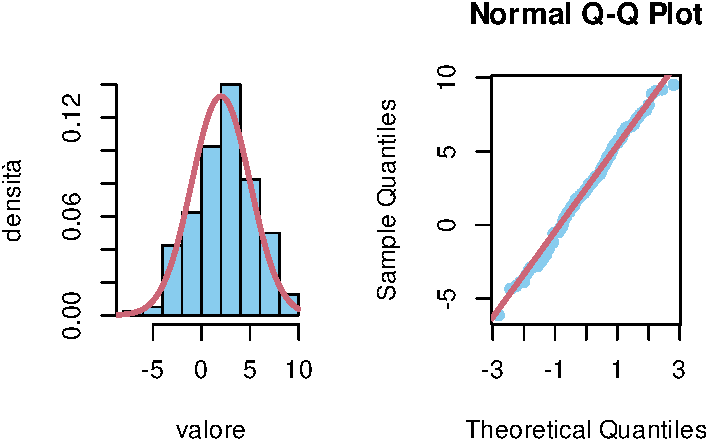
\includegraphics[keepaspectratio]{08-teoremi_limite_files/figure-pdf/unnamed-chunk-5-1.pdf}}

}

\caption{istogramma e qqplot di 200 variabili gaussiane indipendenti}

\end{figure}%

Con opportune estensioni (ad esempio le librerie JAGS o Stan) si può
realizzare variabili con densità più complesse. Le tecniche principali
consistono nel simulare opportune catene di Markov.

Oltre a fornire dati aleatori ma in un certo senso ``controllati'' su
cui testare esempi e metodi, la simulazione di variabili aleatorie può
essere inserita in opportuni algoritmi, che portano il nome di metodi
Monte Carlo, in cui anche problemi che non riguardano la probabilità
sono affrontabili mediante simulazioni di un gran numero di variabili.

Per fare un esempio, si supponga di dover calcolare l'integrale
\[ \int_{\R^d} g(x) p(X=x) d x,\] dove \(g\) e \(p\) sono note e
regolari, ma la dimensione \(d\) è molto elevata. Ricorrendo ad una
simulazione (purche non abbia costi computazionali onerosi) di \(n\)
variabili indipendenti, tutte con densità \(p(X=\cdot)\), allora la
legge dei grandi numeri assicura che per \(n\) grande,
\[ \int_{\R^d} g(x) p(X=x) d x \approx \frac 1 n \sum_{i=1}^n g(X_i),\]
con alta probabilità. Il teorema limite centrale garantisce invece che
le oscillazioni
\[ \int_{\R^d} g(x) p(X=x) d x- \frac 1 n \sum_{i=1}^n g(X_i)\] saranno
circa gaussiane ma con una deviazione standard proporzionale a
\(1/\sqrt{n}\). Il vantaggio di questo metodo, rispetto ad esempio ad
una integrazione numerica deterministica, è che in dimensione alta
(ossia se \(d\) è grande) non è particolarmente più oneroso (mentre in
dimensione bassa è possibile fare di meglio).

\begin{Shaded}
\begin{Highlighting}[]
\NormalTok{n}\OtherTok{=}\DecValTok{1000}

\NormalTok{gaussiane }\OtherTok{=} \FunctionTok{rnorm}\NormalTok{(n)}

\NormalTok{g }\OtherTok{=}\NormalTok{ gaussiane}\SpecialCharTok{\^{}}\DecValTok{2}

\NormalTok{monte\_carlo }\OtherTok{=} \FunctionTok{cumsum}\NormalTok{( g ) }\SpecialCharTok{/} \DecValTok{1}\SpecialCharTok{:}\NormalTok{n}

\FunctionTok{plot}\NormalTok{(}\DecValTok{1}\SpecialCharTok{:}\NormalTok{n, monte\_carlo, }\AttributeTok{type=}\StringTok{\textquotesingle{}l\textquotesingle{}}\NormalTok{, }\AttributeTok{lwd=}\DecValTok{3}\NormalTok{, }\AttributeTok{col=}\NormalTok{miei\_colori[}\DecValTok{2}\NormalTok{], }\AttributeTok{ylab=}\StringTok{\textquotesingle{}approssimazione\textquotesingle{}}\NormalTok{, }\AttributeTok{xlab=}\StringTok{\textquotesingle{}numero simulazioni\textquotesingle{}}\NormalTok{)}

\FunctionTok{abline}\NormalTok{(}\AttributeTok{h=}\DecValTok{1}\NormalTok{, }\AttributeTok{col=}\NormalTok{miei\_colori[}\DecValTok{1}\NormalTok{], }\AttributeTok{lwd=}\DecValTok{3}\NormalTok{)}
\end{Highlighting}
\end{Shaded}

\begin{figure}[H]

{\centering \pandocbounded{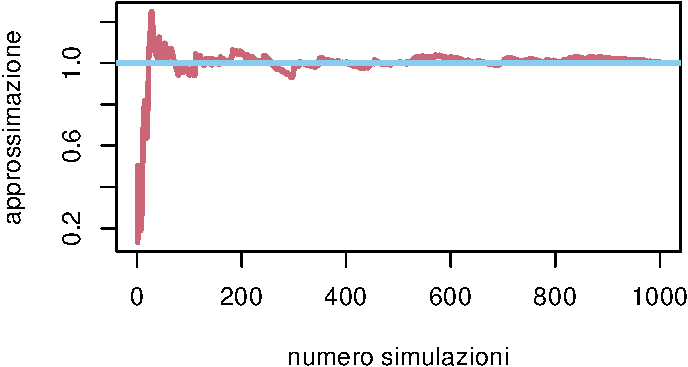
\includegraphics[keepaspectratio]{08-teoremi_limite_files/figure-pdf/unnamed-chunk-6-1.pdf}}

}

\caption{Calcolo del momento secondo di una gaussiana standard tramite
media empirica di un campione indipendente.}

\end{figure}%

\section{Cenni agli eventi estremi}\label{sec-extreme}

Lo studio delle caratteristiche \emph{medie} di una famiglia di
variabili aleatorie (o di un processo) è molto rilevante ai fini
pratici, ma altrettanto può esserlo quello delle caratteristiche
\emph{estreme}: se \((X_t)_{t \in \mathcal{T}}\) indica la temperatura
di un dispositivo il cui funzionamento è garantito se è sempre compresa
in un determinato intervallo di valori, è importante stimare la
probabilità che la temperatura massima (o minima) raggiunta sia al di
fuori di tale intervallo.

Si tratta quindi di sostituire l'operazione di media campionaria con il
massimo tra \(n\) osservazioni \[ M_n = \max_{i=1, \ldots, n} X_i,\] o
il minimo \[ m_n = \min_{i=1, \ldots, n} X_i.\] Supponendo che le
variabili \((X_n)_{n=1}^\infty\) siano indipendenti e tutte con la
stessa legge, si può investigare il limite al tendere di
\(n \to \infty\) delle due variabili. Per brevità consideriamo solamente
il caso del massimo (il caso del minimo è analogo).

Per comprendere \(M_n\) è utile considerarne la \(\CDF\):
\[ \begin{split} \CDF_{M_n}(t) & = P( \max_{i=1, \ldots, n} X_i \le t) \\
& =P( X_1 \le t, X_2 \le t, \ldots, X_n \le t)\\
& = P(X_1 \le t) P(X_2 \le t) \ldots P(X_n \le t).\end{split}\] Nel caso
di densità continue delle \(X_i\), derivando questa identità si trova la
densità di \(M_n\).

Tuttavia, volendo limitarci a teoremi limite sotto ipotesi generali,
supponiamo che tutte le \(X_i\) abbiano la stessa legge (e quindi la
stessa \(\CDF\)) e mostriamo il seguente risultato, analogo per certi
versi alla legge dei grandi numeri.

Siano \((X_n)_{n =1 }^\infty\) variabili aleatorie a valori reali,
indipendenti e tutte con la stessa legge. Se \(t \in \R\) è tale che
\(\CDF_{X_1} (t)<1\), ossia \[ P(X_1 >t) >0,\] allora
\[ \lim_{n \to \infty } P(M_n > t)= 1\] In particolare se \(X_1\) assume
con probabilità positiva (anche piccola) valori arbitrariamente grandi,
allora si ha la convergenza in probabilità di \(M_n\) verso \(+\infty\).

In termini più intuitivi, se non è impossibile che le variabili possano
assumere valori arbitrariamente grandi, allora tali valori prima o poi
si osserveranno. Si tratta di una versione del \emph{paradosso di
Borel}: se una scimmia scrive completamente a caso su una tastiera,
prima o poi si vedranno apparire sullo schermo dei versi di Shakespeare.
Ovviamente non è specificato in quanto tempo ci si aspetta che questo
accada: in media esso è inversamente proporzionale alla probabilità che
l'evento accada, il che può essere estremamente grande.

\begin{proof}
Dalla formula per la \(\CDF_{M_n}\), si ha
\[ P(M_n \le t) =  \CDF_{M_n}(t) = (\CDF_{X_n}(t))^n \to 0\] al tendere
di \(n \to \infty\).
\end{proof}

Il teorema sopra si può rendere più preciso mostrando una versione del
teorema limite centrale nello studio degli eventi estremi. In questo
caso la densità gaussiana è sostituita da altre densità, a seconda della
``pesantezza'' delle code delle \(X_i\), ossia dell'ordine di
infinitesimo di \(P(X_i >t)\). Vediamo ad esempio il caso di variabili
esponenziali. Esse si usano tipicamente per i tempi di vita di
dispositivi, quindi il massimo tra \(n\) sarebbe il tempo in cui \(n\)
dispositivi smettono tutti di funzionare.

Siano \((X_n)_{n=1}^\infty\) variabili aleatorie indipendenti, tutte con
densità esponenziale del medesimo parametro \(\lambda>0\). Allora si ha
la convergenza in legge
\[ \lim_{n \to \infty} M_n - \frac{ \log n}{\lambda} = G,\] dove \(G\) è
una variabile con distribuzione di Gumbel, ossia con funzione di
ripartizione, per \(t \in \R\), \[ \CDF_G(t) = \exp\bra{ - e^{-t}}.\]

La densità di \(G\) si ottiene derivando:
\[ \frac{d}{dt} \CDF_G(t) = \exp\bra{-t-e^{-t}  }.\]

\begin{proof}
Per semplicità supponiamo \(\lambda=1\), il caso generale è simile. Sia
\(t \in \R\) e calcoliamo
\[\CDF_{M_n - \log n}(t) =\CDF_{M_n}(t+\log n) = \bra{ \CDF_{X_1}(t+\log n)}^n.\]
Ricordando che \(\CDF_{X_1}(s) = 1-e^{-s}\) per \(s>0\), e osservando
che \(t+\log n> 0\) se \(n\) è abbastanza grande (anche se \(t\) è
negativo), otteniamo
\[ \bra{ \CDF_{X_1}(t+\log n)}^n = (1- e^{-t-\log n})^n = \bra{ 1 - \frac{e^{-t}}{n}}^n \to e^{-e^{-t}},\]
per \(n \to \infty\).
\end{proof}

\section{Problemi}\label{problemi-5}

\bookmarksetup{startatroot}

\chapter{Introduzione ad R}\label{sec-appR}

In questa appendice diamo qualche informazione introduttiva su R ed
RStudio (a partire da come installarli nel proprio dispositivo).

\section{Installare R ed RStudio}\label{installare-r-ed-rstudio}

\textbf{R} è un linguaggio per il calcolo statistico. È
multipiattaforma, gratuito e aperto (open-source). Dispone di una
comunità molto attiva, molte estensioni (librerie) sono facilmente
reperibili e ben curate -- pur non essendovi una garanzia commerciale.

Perché il nome R? è un'evoluzione open-source di un linguaggio per
statistica chiamato S.

Per installare R sul proprio computer, si seguano le istruzioni per
scaricare una distribuzione pre-compilate alla pagina
\url{https://cran.rstudio.com/}.

Oltre ad R, è fortemente consigliato installare inoltre \textbf{RStudio}
che fornisce una interfaccia grafica ed un editor di testo con funzioni
avanzate (precisamente è un \emph{Integrated Development Enviroment},
IDE), che ne agevola notevolmente l'uso. La versione Desktop di RStudio
è open-source e liberamente scaricabile seguendo le istruzioni alla
pagina \url{https://rstudio.com/products/rstudio/download/\#download}.

\section{Primi comandi}\label{primi-comandi}

All'avvio di Rstudio appare un terminale (in basso a sinistra) in cui
possiamo inserire del testo. Questo ci permette di dialogare
direttamente con una sessione di R.

Possiamo scrivere un file contenente comandi da eseguire cliccando su
\emph{File-\textgreater New File-\textgreater R script} Questo produce
uno script (una lista di comandi da eseguire).

In alternativa, possiamo anche procedere con \emph{File-\textgreater New
File-\textgreater R notebook}, che produce un file di testo contenente
blocchi di comandi eseguibili, esportabile in svariati formati, come
HTML o PDF. Questo è molto utile se dovete preparare un report con
l'analisi di alcuni dati (oppure documenti più sofisticati, ad esempio
questi appunti sono tutti scritti usando R bookdown, una evoluzione di R
notebook per scrivere libri).

Per gestire \emph{progetti} più complessi, contenenti diversi files,
conviene andare alla voce \emph{File-\textgreater New Project\ldots{}}

In generale si può ottenere informazioni su un comando digitandolo
preceduto dal punto interrogativo. Ad esempio \texttt{?exp} fornisce
indicazioni sul comando \texttt{exp()}. Dal menù \emph{Help} si può
accedere a svariate risorse, tutorial e documentazione per conoscere
comandi di base e più avanzati.

\section{R come calcolatrice}\label{r-come-calcolatrice}

Il primo uso che possiamo fare di R è una calcolatrice in cui molte
funzioni e costanti matematiche sono già disponibili.

\begin{Shaded}
\begin{Highlighting}[]
\DecValTok{3}\SpecialCharTok{+}\DecValTok{4}\SpecialCharTok{*}\NormalTok{(}\DecValTok{1}\SpecialCharTok{+}\DecValTok{2}\NormalTok{)}
\end{Highlighting}
\end{Shaded}

\begin{verbatim}
[1] 15
\end{verbatim}

\begin{Shaded}
\begin{Highlighting}[]
\DecValTok{2}\SpecialCharTok{\^{}}\DecValTok{2}
\end{Highlighting}
\end{Shaded}

\begin{verbatim}
[1] 4
\end{verbatim}

\begin{Shaded}
\begin{Highlighting}[]
\DecValTok{2}\SpecialCharTok{**}\DecValTok{2}
\end{Highlighting}
\end{Shaded}

\begin{verbatim}
[1] 4
\end{verbatim}

\begin{Shaded}
\begin{Highlighting}[]
\FunctionTok{sqrt}\NormalTok{(}\DecValTok{2}\NormalTok{)}
\end{Highlighting}
\end{Shaded}

\begin{verbatim}
[1] 1.414214
\end{verbatim}

\begin{Shaded}
\begin{Highlighting}[]
\DecValTok{2}\SpecialCharTok{**}\NormalTok{(}\DecValTok{1}\SpecialCharTok{/}\DecValTok{2}\NormalTok{)}
\end{Highlighting}
\end{Shaded}

\begin{verbatim}
[1] 1.414214
\end{verbatim}

\begin{Shaded}
\begin{Highlighting}[]
\NormalTok{pi}
\end{Highlighting}
\end{Shaded}

\begin{verbatim}
[1] 3.141593
\end{verbatim}

\begin{Shaded}
\begin{Highlighting}[]
\FunctionTok{sin}\NormalTok{(pi)}
\end{Highlighting}
\end{Shaded}

\begin{verbatim}
[1] 1.224647e-16
\end{verbatim}

\begin{Shaded}
\begin{Highlighting}[]
\FunctionTok{exp}\NormalTok{( }\FunctionTok{log}\NormalTok{ (}\DecValTok{2}\NormalTok{) )}
\end{Highlighting}
\end{Shaded}

\begin{verbatim}
[1] 2
\end{verbatim}

\begin{Shaded}
\begin{Highlighting}[]
\FunctionTok{log}\NormalTok{(}\DecValTok{0}\NormalTok{)}
\end{Highlighting}
\end{Shaded}

\begin{verbatim}
[1] -Inf
\end{verbatim}

\begin{Shaded}
\begin{Highlighting}[]
\DecValTok{0}\SpecialCharTok{/}\DecValTok{1}
\end{Highlighting}
\end{Shaded}

\begin{verbatim}
[1] 0
\end{verbatim}

\begin{Shaded}
\begin{Highlighting}[]
\DecValTok{1}\SpecialCharTok{/}\DecValTok{0}
\end{Highlighting}
\end{Shaded}

\begin{verbatim}
[1] Inf
\end{verbatim}

\begin{Shaded}
\begin{Highlighting}[]
\DecValTok{0}\SpecialCharTok{/}\DecValTok{0}
\end{Highlighting}
\end{Shaded}

\begin{verbatim}
[1] NaN
\end{verbatim}

\section{Oggetti}\label{oggetti}

Il linguaggio permette di introdurre oggetti (numeri, vettori, liste,
funzioni\ldots) e li mantiene in memoria fino alla chiusura di una
sessione, a meno che non vengano esplicitamente rimossi (questo può
essere utile per le prestazioni nel caso si usi troppa memoria).

Per vedere quali oggetti sono attualmente disponibili nell'ambiente,
usiamo il comando \texttt{ls()} oppure nella sezione in alto a destra,
clicchiamo su \emph{Environment}.

Possiamo definire oggetti con il nome che preferiamo con i comandi
\texttt{=} oppure \texttt{\textless{}-} (in R è buona pratica usare il
secondo, ma il simbolo di uguaglianza è comune a molti altri linguaggi).
Definiamo ad esempio un oggetto numerico \(X\) assegnando il valore 3:

\begin{Shaded}
\begin{Highlighting}[]
\NormalTok{X }\OtherTok{=} \DecValTok{3}
\end{Highlighting}
\end{Shaded}

oppure equivalentemente possiamo anche digitare \texttt{X\ =\ 3}. Per
accedere al valore, basta dare il suo nome come comando

\begin{Shaded}
\begin{Highlighting}[]
\NormalTok{X}
\end{Highlighting}
\end{Shaded}

\begin{verbatim}
[1] 3
\end{verbatim}

Osserviamo che se introduciamo una copia \(Y\) di \(X\) e poi
modifichiamo il valore di \(X\), \(Y\) non cambia.

\begin{Shaded}
\begin{Highlighting}[]
\NormalTok{Y }\OtherTok{=}\NormalTok{ X}

\NormalTok{X }\OtherTok{=} \DecValTok{4}

\NormalTok{Y}
\end{Highlighting}
\end{Shaded}

\begin{verbatim}
[1] 3
\end{verbatim}

Le operazioni tra oggetti (numerici) sono abbastanza naturali:

\begin{Shaded}
\begin{Highlighting}[]
\NormalTok{x0 }\OtherTok{=} \DecValTok{1}
\NormalTok{x1 }\OtherTok{=} \DecValTok{5}
\NormalTok{x2 }\OtherTok{=} \DecValTok{7}

\NormalTok{somma }\OtherTok{=}\NormalTok{ x0}\SpecialCharTok{+}\NormalTok{x1}\SpecialCharTok{+}\NormalTok{x2}

\NormalTok{somma}
\end{Highlighting}
\end{Shaded}

\begin{verbatim}
[1] 13
\end{verbatim}

\begin{Shaded}
\begin{Highlighting}[]
\NormalTok{prodotto }\OtherTok{=}\NormalTok{ x0 }\SpecialCharTok{*}\NormalTok{ x1 }\SpecialCharTok{*}\NormalTok{ x2}

\NormalTok{prodotto}
\end{Highlighting}
\end{Shaded}

\begin{verbatim}
[1] 35
\end{verbatim}

Ci sono diversi tipi di oggetti, per conoscerne il tipo (la classe) il
comando è \texttt{class()}, con il nome dell'oggetto tra le parentesi.
Ad esempio,

\begin{Shaded}
\begin{Highlighting}[]
\FunctionTok{class}\NormalTok{(X)}
\end{Highlighting}
\end{Shaded}

\begin{verbatim}
[1] "numeric"
\end{verbatim}

\section{Logical e character}\label{logical-e-character}

Una classe di oggetti utile sono i \textbf{LOGICAL} (valori TRUE o
FALSE).

\begin{Shaded}
\begin{Highlighting}[]
\FunctionTok{class}\NormalTok{(}\ConstantTok{TRUE}\NormalTok{)}
\end{Highlighting}
\end{Shaded}

\begin{verbatim}
[1] "logical"
\end{verbatim}

Le operazioni Booleane sono \texttt{\&} (and), \texttt{\textbar{}} (or),
\texttt{!} (not).

\begin{Shaded}
\begin{Highlighting}[]
\ConstantTok{TRUE} \SpecialCharTok{\&} \ConstantTok{FALSE}
\end{Highlighting}
\end{Shaded}

\begin{verbatim}
[1] FALSE
\end{verbatim}

\begin{Shaded}
\begin{Highlighting}[]
\ConstantTok{TRUE} \SpecialCharTok{|} \ConstantTok{FALSE}
\end{Highlighting}
\end{Shaded}

\begin{verbatim}
[1] TRUE
\end{verbatim}

\begin{Shaded}
\begin{Highlighting}[]
\SpecialCharTok{!}\ConstantTok{TRUE}
\end{Highlighting}
\end{Shaded}

\begin{verbatim}
[1] FALSE
\end{verbatim}

Possiamo inoltre confrontare due oggetti numerici usando \texttt{==} per
verificare se coincidono

\begin{Shaded}
\begin{Highlighting}[]
\DecValTok{1} \SpecialCharTok{==} \DecValTok{1} 
\end{Highlighting}
\end{Shaded}

\begin{verbatim}
[1] TRUE
\end{verbatim}

\begin{Shaded}
\begin{Highlighting}[]
\DecValTok{1} \SpecialCharTok{\textgreater{}=} \DecValTok{2}
\end{Highlighting}
\end{Shaded}

\begin{verbatim}
[1] FALSE
\end{verbatim}

\begin{Shaded}
\begin{Highlighting}[]
\DecValTok{1} \SpecialCharTok{!=} \DecValTok{2}
\end{Highlighting}
\end{Shaded}

\begin{verbatim}
[1] TRUE
\end{verbatim}

Un`altra classe di oggetti sono i \textbf{CHARACTER}, ossia stringhe di
caratteri evidenziate dalla presenza delle virgolette.

\begin{Shaded}
\begin{Highlighting}[]
\NormalTok{X }\OtherTok{=} \StringTok{\textquotesingle{}hello world\textquotesingle{}}

\FunctionTok{print}\NormalTok{(}\StringTok{\textquotesingle{}hello world\textquotesingle{}}\NormalTok{)}
\end{Highlighting}
\end{Shaded}

\begin{verbatim}
[1] "hello world"
\end{verbatim}

\section{Vettori}\label{vettori}

I dati raccolti sperimentalmente spesso sono sequenze di osservazioni
(ad esempio corrispondenti a diversi istanti nel tempo) che possiamo
rappresentare come vettori. Per costruire un vettore usiamo la funzione
di \emph{concatenazione} \texttt{c()}.

\begin{Shaded}
\begin{Highlighting}[]
\NormalTok{vettore }\OtherTok{=} \FunctionTok{c}\NormalTok{(}\DecValTok{1}\NormalTok{,}\DecValTok{2}\NormalTok{,}\DecValTok{3}\NormalTok{)}

\NormalTok{vettore}
\end{Highlighting}
\end{Shaded}

\begin{verbatim}
[1] 1 2 3
\end{verbatim}

In realtà R non distingue tra vettore e scalare. Questo è utile ad
esempio per le operazioni matematiche che vengono eseguite su ciancun
elemento.

\begin{Shaded}
\begin{Highlighting}[]
\NormalTok{vettore }\SpecialCharTok{*} \DecValTok{2}
\end{Highlighting}
\end{Shaded}

\begin{verbatim}
[1] 2 4 6
\end{verbatim}

\begin{Shaded}
\begin{Highlighting}[]
\NormalTok{vettore }\SpecialCharTok{+}\NormalTok{ vettore}
\end{Highlighting}
\end{Shaded}

\begin{verbatim}
[1] 2 4 6
\end{verbatim}

\begin{Shaded}
\begin{Highlighting}[]
\NormalTok{vettore }\SpecialCharTok{*}\NormalTok{ vettore}
\end{Highlighting}
\end{Shaded}

\begin{verbatim}
[1] 1 4 9
\end{verbatim}

\begin{Shaded}
\begin{Highlighting}[]
\FunctionTok{exp}\NormalTok{( vettore )}
\end{Highlighting}
\end{Shaded}

\begin{verbatim}
[1]  2.718282  7.389056 20.085537
\end{verbatim}

Attenzione però quando operiamo con vettori di lunghezze diverse:

\begin{Shaded}
\begin{Highlighting}[]
\NormalTok{vettore0 }\OtherTok{=} \FunctionTok{c}\NormalTok{(}\DecValTok{1}\NormalTok{,}\DecValTok{2}\NormalTok{,}\DecValTok{3}\NormalTok{,}\DecValTok{4}\NormalTok{)}

\NormalTok{vettore0}
\end{Highlighting}
\end{Shaded}

\begin{verbatim}
[1] 1 2 3 4
\end{verbatim}

\begin{Shaded}
\begin{Highlighting}[]
\NormalTok{vettore1}\OtherTok{=} \FunctionTok{c}\NormalTok{(}\DecValTok{1}\NormalTok{,}\DecValTok{2}\NormalTok{)}

\NormalTok{vettore1}
\end{Highlighting}
\end{Shaded}

\begin{verbatim}
[1] 1 2
\end{verbatim}

\begin{Shaded}
\begin{Highlighting}[]
\NormalTok{vettore0 }\SpecialCharTok{+}\NormalTok{ vettore1}
\end{Highlighting}
\end{Shaded}

\begin{verbatim}
[1] 2 4 4 6
\end{verbatim}

\begin{Shaded}
\begin{Highlighting}[]
\NormalTok{vettore0}\SpecialCharTok{*}\NormalTok{vettore1}
\end{Highlighting}
\end{Shaded}

\begin{verbatim}
[1] 1 4 3 8
\end{verbatim}

Possiamo selezionare gli elementi di un vettore specificandone la
posizione tra parentesi quadre \texttt{{[}{]}}.

\begin{Shaded}
\begin{Highlighting}[]
\NormalTok{vettore }\OtherTok{=} \FunctionTok{c}\NormalTok{(}\DecValTok{5}\NormalTok{,}\DecValTok{3}\NormalTok{,}\DecValTok{6}\NormalTok{,}\DecValTok{18}\NormalTok{,}\SpecialCharTok{{-}}\DecValTok{1}\NormalTok{)}

\NormalTok{vettore[}\DecValTok{1}\NormalTok{]}
\end{Highlighting}
\end{Shaded}

\begin{verbatim}
[1] 5
\end{verbatim}

\begin{Shaded}
\begin{Highlighting}[]
\NormalTok{vettore[}\DecValTok{2}\NormalTok{]}
\end{Highlighting}
\end{Shaded}

\begin{verbatim}
[1] 3
\end{verbatim}

\textbf{Attenzione}: diversamente da altri linguaggi, R conta le
posizioni a partire da \(1\), non da \(0\).

Possiamo anche inserire un vettore all'interno delle parentesi quadre
per selezionare un sottovettore del vettore iniziale. Oppure inserire un
vettore di oggetti LOGICAL, in tal caso si seleziona il sottovettore
corrispondente alle componenti \texttt{TRUE}.

\begin{Shaded}
\begin{Highlighting}[]
\NormalTok{vettore[}\FunctionTok{c}\NormalTok{(}\DecValTok{1}\NormalTok{,}\DecValTok{2}\NormalTok{,}\DecValTok{5}\NormalTok{)]}
\end{Highlighting}
\end{Shaded}

\begin{verbatim}
[1]  5  3 -1
\end{verbatim}

\begin{Shaded}
\begin{Highlighting}[]
\NormalTok{vettore }\SpecialCharTok{\textgreater{}=} \DecValTok{5}
\end{Highlighting}
\end{Shaded}

\begin{verbatim}
[1]  TRUE FALSE  TRUE  TRUE FALSE
\end{verbatim}

\begin{Shaded}
\begin{Highlighting}[]
\NormalTok{vettore[ vettore }\SpecialCharTok{\textgreater{}=} \DecValTok{5}\NormalTok{]}
\end{Highlighting}
\end{Shaded}

\begin{verbatim}
[1]  5  6 18
\end{verbatim}

\begin{Shaded}
\begin{Highlighting}[]
\DecValTok{1}\SpecialCharTok{:}\DecValTok{4}
\end{Highlighting}
\end{Shaded}

\begin{verbatim}
[1] 1 2 3 4
\end{verbatim}

\begin{Shaded}
\begin{Highlighting}[]
\NormalTok{vettore[}\DecValTok{1}\SpecialCharTok{:}\DecValTok{4}\NormalTok{]}
\end{Highlighting}
\end{Shaded}

\begin{verbatim}
[1]  5  3  6 18
\end{verbatim}

Per creare un vettore di numeri reali equispaziati usiamo il comando
\texttt{seq()}.

\begin{Shaded}
\begin{Highlighting}[]
\NormalTok{x }\OtherTok{=} \FunctionTok{seq}\NormalTok{(}\SpecialCharTok{{-}}\DecValTok{1}\NormalTok{, }\DecValTok{1}\NormalTok{, }\AttributeTok{by=}\FloatTok{0.1}\NormalTok{)}

\NormalTok{x}
\end{Highlighting}
\end{Shaded}

\begin{verbatim}
 [1] -1.0 -0.9 -0.8 -0.7 -0.6 -0.5 -0.4 -0.3 -0.2 -0.1  0.0
[12]  0.1  0.2  0.3  0.4  0.5  0.6  0.7  0.8  0.9  1.0
\end{verbatim}

\section{Plot, barplot e istogrammi}\label{plot-barplot-e-istogrammi}

Il comando \texttt{plot()} è il comando di base per rappresentare
grafici in due dimensioni. Usiamolo ad esempio per tracciare un grafico
della funzione \(\sin(x)\) nell'intervallo \([0, 2\pi]\).

\begin{Shaded}
\begin{Highlighting}[]
\NormalTok{deltax}\OtherTok{=}\FloatTok{0.01}
\NormalTok{x }\OtherTok{=} \FunctionTok{seq}\NormalTok{(}\DecValTok{0}\NormalTok{,}\DecValTok{2}\SpecialCharTok{*}\NormalTok{pi, }\AttributeTok{by=}\NormalTok{deltax)}

\NormalTok{y }\OtherTok{=} \FunctionTok{sin}\NormalTok{(x)}

\FunctionTok{plot}\NormalTok{(x,y, }\AttributeTok{type=}\StringTok{\textquotesingle{}l\textquotesingle{}}\NormalTok{)}
\end{Highlighting}
\end{Shaded}

\begin{center}
\pandocbounded{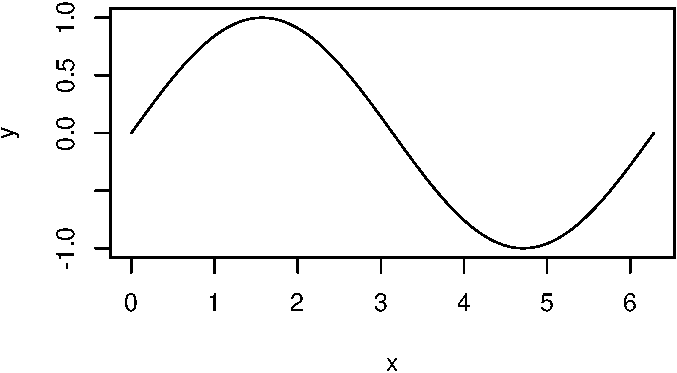
\includegraphics[keepaspectratio]{10-R-intro_files/figure-pdf/unnamed-chunk-18-1.pdf}}
\end{center}

Possiamo aggiungiamo delle etichette agli assi e cambiare il colore al
grafico, ad esempio

\begin{Shaded}
\begin{Highlighting}[]
\FunctionTok{plot}\NormalTok{(x, y, }\AttributeTok{type=}\StringTok{\textquotesingle{}l\textquotesingle{}}\NormalTok{, }\AttributeTok{xlab=}\StringTok{\textquotesingle{}x\textquotesingle{}}\NormalTok{, }\AttributeTok{ylab=}\StringTok{\textquotesingle{}sin(x)\textquotesingle{}}\NormalTok{,  }\AttributeTok{col=}\NormalTok{miei\_colori[}\DecValTok{1}\NormalTok{], }\AttributeTok{lwd=}\DecValTok{3}\NormalTok{, }\AttributeTok{main=}\StringTok{"grafico della funzione seno"}\NormalTok{)}
\end{Highlighting}
\end{Shaded}

\begin{center}
\pandocbounded{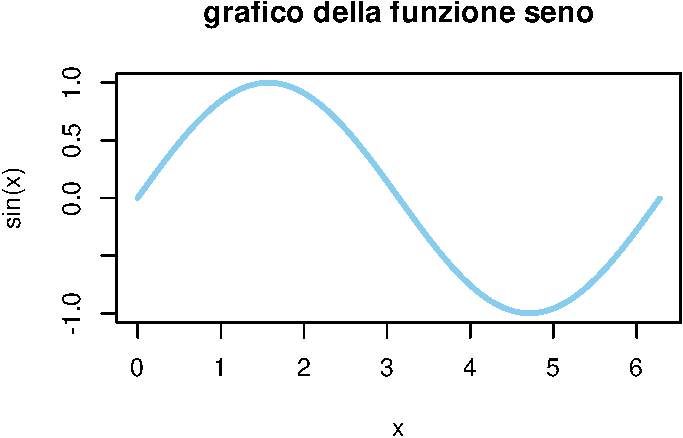
\includegraphics[keepaspectratio]{10-R-intro_files/figure-pdf/unnamed-chunk-19-1.pdf}}
\end{center}

Per rappresentare grafici a barre il comando è \texttt{barplot()}:

\begin{Shaded}
\begin{Highlighting}[]
\FunctionTok{barplot}\NormalTok{( }\DecValTok{1}\SpecialCharTok{:}\DecValTok{4}\NormalTok{, }\AttributeTok{col=}\NormalTok{miei\_colori[}\DecValTok{1}\NormalTok{], }\AttributeTok{names.arg =} \FunctionTok{c}\NormalTok{(}\StringTok{"uno"}\NormalTok{, }\StringTok{"due"}\NormalTok{, }\StringTok{"tre"}\NormalTok{, }\StringTok{"quattro"}\NormalTok{))}
\end{Highlighting}
\end{Shaded}

\begin{center}
\pandocbounded{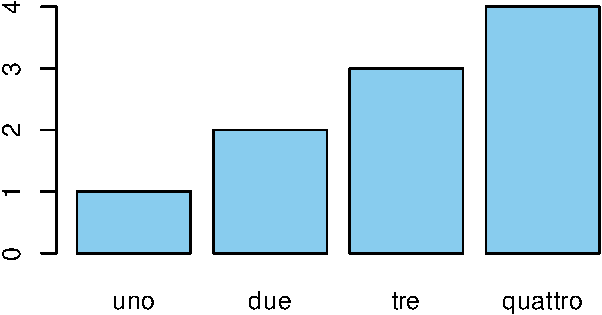
\includegraphics[keepaspectratio]{10-R-intro_files/figure-pdf/unnamed-chunk-20-1.pdf}}
\end{center}

per rappresentare istogrammi (ossia diagrammi a barre delle frequenze in
cui un insieme di dati assume valori in determinati intervalli), il
comando è \texttt{hist()}:

\begin{Shaded}
\begin{Highlighting}[]
\FunctionTok{hist}\NormalTok{(y, }\AttributeTok{col=}\NormalTok{miei\_colori[}\DecValTok{1}\NormalTok{])}
\end{Highlighting}
\end{Shaded}

\begin{center}
\pandocbounded{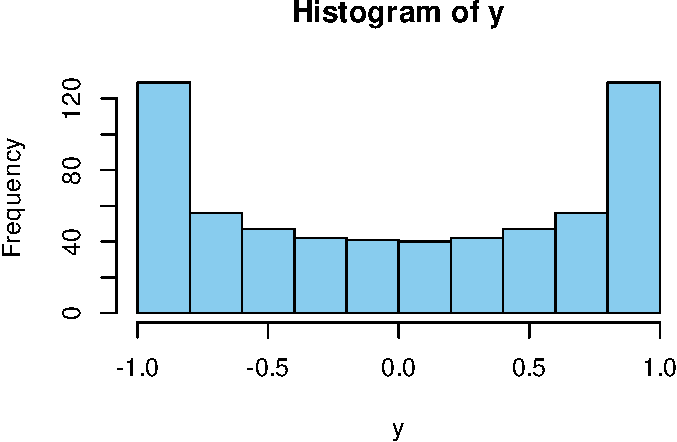
\includegraphics[keepaspectratio]{10-R-intro_files/figure-pdf/unnamed-chunk-21-1.pdf}}
\end{center}

\section{Pacchetti}\label{pacchetti}

Uno dei punti di forza di R è l'ampia disponibilità di pacchetti (o
librerie) che contengono svariate funzioni pronte all'uso per l'analisi
dei dati, la rappresentazione grafica e la statistica. Faremo uso di
qualche pacchetto anche nel corso. Il comando di base per
\emph{installare} un pacchetto (assicurarsi di essere connessi ad
Internet) è \texttt{install.packages()} dove bisogna specificare tra
virgolette il nome del pacchetto che si vuole installare. Ad esempio,
faremo uso di \texttt{forecast}, perciò si può installarlo digitando
sulla console di R
\texttt{install.packages(\textquotesingle{}forecast\textquotesingle{})}.

Per \emph{caricare} in una sessione di R un pacchetto e quindi poter
accedere a tutte le funzioni che contiene, il comando è
\texttt{library()} in cui di nuovo bisogna specificare nelle parentesi
il nome del pacchetto di interesse. Perciò per poter accedere alle
funzioni di \texttt{forecast} basterà digitare, dopo averlo installato
correttamente, il comando \texttt{library(forecast)}. Non è necessario
installare ogni volta il pacchetto, mentre in ogni sessione di R vanno
caricati ogni volta (a meno di non riprendere una sessione già salvata).

Se si vuole accedere solo ad una funzione da un pacchetto installato (ma
non necessariamente caricato con \texttt{library()}), basta digitare il
nome del pacchetto, due volte due punti, \texttt{::}, e poi il nome
della funzione. Ad esempio, per usare la funzione \texttt{Acf()} dal
pacchetto \texttt{forecast} (supponendo che sia installato), basta
digitare \texttt{forecast::Acf()}.

Un elenco dei pacchetti disponibili è mantenuto sul sito
\href{https://cran.r-project.org/web/packages/available_packages_by_name.html}{CRAN}.

Le funzioni descritte sopra sono sufficienti per un uso di base, ma per
un uso più efficiente dei pacchetti e in particolare la gestione delle
interdipendenze (una funzione può avere bisogno di altre funzioni
definite in altri pacchetti ecc.), consigliamo il tool
\href{https://cran.r-project.org/web/packages/pacman/index.html}{pacman}.
Per installarlo basta dare il comando
\texttt{install.packages(\textquotesingle{}pacman\textquotesingle{})}.

\section{Input e Output}\label{input-e-output}

La gestione dell'input e dell'output (ad esempio di previsioni, stime
ecc.) in R può essere un po' noiosa, perché formati di file diversi
(testo semplice, Excel, ecc.) richiedono comandi diversi. Tuttavia, per
un uso di base, si può installare il pacchetto \texttt{rio}. Consigliamo
di usare \texttt{pacman} come strumento per l'installazione. Digitare
quindi
\texttt{install.packages(\textquotesingle{}pacman\textquotesingle{})} se
\texttt{pacman} non è già installato. Successivamente, basta digitare
\texttt{pacman::p\_install(\textquotesingle{}rio\textquotesingle{})} per
installarlo e
\texttt{pacman::p\_load(\textquotesingle{}rio\textquotesingle{})} per
caricarlo.

Una volta caricato, i comandi principali sono \texttt{import()} ed
\texttt{export()} rispettivamente per caricare da un file e salvare dei
dati su un file. È importante specificare l'estensione del file (si basa
su quello per determinare il tipo di file).

Non tutti i formati sono supportati di base (in particolare gli Excel
non lo sono), si veda la descrizione a
\href{https://cran.r-project.org/web/packages/rio/vignettes/rio.html}{questa
pagina} (bisogna usare il comando \texttt{install\_formats()})

\begin{Shaded}
\begin{Highlighting}[]
\CommentTok{\# Carichiamo rio}

\FunctionTok{library}\NormalTok{(}\StringTok{\textquotesingle{}rio\textquotesingle{}}\NormalTok{)}

\CommentTok{\# Esportiamo il dataset Iris come un file .csv (comma separated value), ossia un file di testo semplice in cui le colonne sono separate da virgola}

\FunctionTok{export}\NormalTok{(iris, }\StringTok{"iris.csv"}\NormalTok{)}

\CommentTok{\# Nella cartella di lavoro dovrebbe essere presente il file iris.csv. Per importare basta usare il comando import. Vediamo ad esempio sullo stesso file appena creato}

\NormalTok{iris\_importato }\OtherTok{=} \FunctionTok{import}\NormalTok{( }\StringTok{"iris.csv"}\NormalTok{)}

\CommentTok{\# Riconosciamo il solito dataset Iris}

\FunctionTok{head}\NormalTok{(iris\_importato)}
\end{Highlighting}
\end{Shaded}

\begin{verbatim}
  Sepal.Length Sepal.Width Petal.Length Petal.Width Species
1          5.1         3.5          1.4         0.2  setosa
2          4.9         3.0          1.4         0.2  setosa
3          4.7         3.2          1.3         0.2  setosa
4          4.6         3.1          1.5         0.2  setosa
5          5.0         3.6          1.4         0.2  setosa
6          5.4         3.9          1.7         0.4  setosa
\end{verbatim}

\subsection{Esercizi}\label{esercizi-40}

Approssimare numericamente l'integrale di \(\sin(x)\) nell'intervallo
\([1/2,1]\). Può essere utile il comando \texttt{sum()}.

Perché il grafico prodotto dal comando \texttt{hist(y)} sopra non mostra
barre della medesima altezza? Ripetere la stessa costruzione con una
funzione \(y= f(x)\) diversa: per quali valori di \(y\) l'istogramma
presenterà barre più alte?

\bookmarksetup{startatroot}

\chapter{Richiami sulla trasformata di Fourier}\label{sec-fourier}

In questa appendice richiamiamo alcune notazioni e risultati principali
riguardanti la trasformata di Fourier, prima nel caso finito (Sezione
Sezione~\ref{sec-fourier-finita}) poi nel caso di tempi discreti
(Sezione Sezione~\ref{sec-fourier-discreta}) e infine nel caso continuo
(Sezione Sezione~\ref{sec-fourier-continua})

\section{Caso finito}\label{sec-fourier-finita}

Fissano \(n \in \N\), si consideri un \emph{segnale} definito (o
misurato) su un intervallo discreto di \(n\) valori
\[g : \cur{0, 1, \ldots, (n-1)} \to \mathbb{C}, \quad t \mapsto g( t ).\]
Si definisce la sua \emph{trasformata di Fourier} come la funzione
\[ \hat g : \cur{0, 1, \ldots, (n-1)}  \to \mathbb{C}, \quad \xi \mapsto  \hat{g}(\xi) := \sum_{t=0}^{n-1} g(t) e^{ - 2 \pi i t \xi/n}.\]

\begin{remark}
Il dominio di definizione della \(g\) può essere pensato come un insieme
di tempi, mentre il dominio di \(\hat{g}\) quello di opportune
\emph{frequenze} \(\xi\) per le funzioni oscillanti
\(t \mapsto e^{ - 2 \pi i t \xi/n}\). Precisamente, le frequenze
sarebbero \(\xi/n\), mentre le frequenze angolari \(2 \pi \xi/n\):
questo giustifica parametrizzazioni diverse della trasformata di
Fourier, ma nel caso discreto quella introdotta sopra è la più comune.
\end{remark}

Se si interpeta sia \(g = (g(t))_{t=0}^{n-1}\) che
\((\hat g(\xi))_{\xi =0}^{n-1}\) come vettori in \(\mathbb{C}^n\),
allora \(\hat{g}\) è il vettore ottenuto moltiplicando \(g\) per la
matrice \(F \in \mathbb{C}^{n\times n}\), data da
\[ F_{\xi t } = e^{ - 2 \pi i t \xi/n}.\] La proprietà fondamentale
della matrice \(F\) è di essere \emph{unitaria}, ossia l'inversa di
\(F\) è la sua trasposta coniugata (in realtà, per via della definizione
che abbiamo usato, questo è vero a meno di una costante moltiplicativa
\(1/n\)). Questo perché vale la relazione di ortogonalità, per \(s\),
\(t \in \cur{0,1, \ldots, n-1}\),
\[  (\bar{F}^T F)_{s t} = \sum_{\xi = 0}^{n-1} e^{  2 \pi i s \xi/n}e^{ - 2 \pi i t \xi/n} = \begin{cases}  n & \text{se $s=t$}\\
 0 &\text{altrimenti.}
 \end{cases}\] Per dimostrarlo basta ricordare la somma geometrica
\(\sum_{j=0}^{k-1} z^j = (z^{k}-1)/(z-1)\) e il fatto che
\(e^{2\pi i }= 1\).

Come prima conseguenza otteniamo allora la formula di inversione
\[ g = \frac{1}{n} \bar{F}^T F g,\] che esplicitamente diventa
\[ g(t ) = \frac 1 n \sum_{\xi=0}^{n-1} \hat{g}(\xi) e^{2 \pi i \xi t/n}.\]
In altre parole, la trasformata di Fourier permette di ricostruire
esattamente \(g\) mediante una operazione inversa che è analoga a quella
diretta.

Una seconda conseguenza è il fatto che la norma (Euclidea) del vettore
\(g\) coincide (a meno di un fattore \(1/n\)) con quella del vettore
\(\hat{g}\), perché
\[ |\hat g|^2 = \overline{F g}^T F g = \bar g^T \bar{F}^T F g = n \bar{g}^T g =   n  |g|^2.\]

\begin{remark}
La norma \(|g|^2\) può essere intepretata come una \emph{energia} del
segnale \(g\), di conseguenza l'identità sopra mostra che la stessa
energia può essere ottenuta sommando le energie associate alle singole
frequenze, ossia \(|\hat{g}(\xi)|^2\) (e dividendo per \(n\)).
\end{remark}

\begin{remark}
Tutte le trasformate di Fourier che si approssimano numericamente sono
ridotte al caso di tempi finiti. Per questo vi sono algoritmi
particolarmente veloci, che in R si possono usare mediante la funzione
\texttt{fft()}. Ecco un esempio.

\begin{Shaded}
\begin{Highlighting}[]
\CommentTok{\# fissiamo n }

\NormalTok{n}\OtherTok{=}\DecValTok{16}

\CommentTok{\#definiamo un vettore dei tempi e uno delle frequenze}

\NormalTok{t }\OtherTok{=} \DecValTok{0}\SpecialCharTok{:}\NormalTok{(n}\DecValTok{{-}1}\NormalTok{)}
\NormalTok{xi}\OtherTok{=} \DecValTok{0}\SpecialCharTok{:}\NormalTok{(n}\DecValTok{{-}1}\NormalTok{)}

\CommentTok{\#questa opzione permette di visualizzare due grafici uno accanto all\textquotesingle{}altro (1,2)=(1 riga, 2 colonne)}

\FunctionTok{par}\NormalTok{(}\AttributeTok{mfrow=}\FunctionTok{c}\NormalTok{(}\DecValTok{1}\NormalTok{,}\DecValTok{2}\NormalTok{))}

\CommentTok{\# definiamo g come l\textquotesingle{}onda quadra e la plottiamo}

\NormalTok{g }\OtherTok{=} \FunctionTok{c}\NormalTok{(}\FunctionTok{rep}\NormalTok{(}\DecValTok{1}\NormalTok{,n}\SpecialCharTok{/}\DecValTok{2}\NormalTok{), }\FunctionTok{rep}\NormalTok{(}\SpecialCharTok{{-}}\DecValTok{1}\NormalTok{, n}\SpecialCharTok{/}\DecValTok{2}\NormalTok{))}

\FunctionTok{plot}\NormalTok{(t, g, }\AttributeTok{col=}\NormalTok{miei\_colori[}\DecValTok{1}\NormalTok{], }\AttributeTok{lwd=}\DecValTok{3}\NormalTok{, }\AttributeTok{pch=}\DecValTok{16}\NormalTok{)}

\CommentTok{\# usiamo fft() per calcolare la trasformata di Fourier e la plottiamo}

\NormalTok{hat\_g }\OtherTok{=} \FunctionTok{fft}\NormalTok{(g)}

\NormalTok{m }\OtherTok{=} \FunctionTok{max}\NormalTok{(}\FunctionTok{abs}\NormalTok{(hat\_g))}

\FunctionTok{plot}\NormalTok{(xi, }\FunctionTok{Re}\NormalTok{(hat\_g), }\AttributeTok{col=}\NormalTok{miei\_colori[}\DecValTok{2}\NormalTok{], }\AttributeTok{ylab=}\StringTok{"trasformata di g"}\NormalTok{, }\AttributeTok{pch=}\DecValTok{16}\NormalTok{, }\AttributeTok{lwd=}\DecValTok{3}\NormalTok{, }\AttributeTok{ylim=}\FunctionTok{c}\NormalTok{(}\SpecialCharTok{{-}}\NormalTok{m,m))}
\FunctionTok{points}\NormalTok{(xi, }\FunctionTok{Im}\NormalTok{(hat\_g)}\SpecialCharTok{+}\FloatTok{0.1}\NormalTok{, }\AttributeTok{col=}\NormalTok{miei\_colori[}\DecValTok{3}\NormalTok{], }\AttributeTok{pch=}\DecValTok{16}\NormalTok{, }\AttributeTok{lwd=}\DecValTok{3}\NormalTok{)}
\FunctionTok{legend}\NormalTok{(}\StringTok{\textquotesingle{}bottomright\textquotesingle{}}\NormalTok{, }\FunctionTok{c}\NormalTok{(}\StringTok{"parte reale"}\NormalTok{, }\StringTok{"parte immaginaria"}\NormalTok{), }\AttributeTok{fill=}\NormalTok{miei\_colori[}\DecValTok{2}\SpecialCharTok{:}\DecValTok{3}\NormalTok{], }\AttributeTok{cex=}\FloatTok{0.7}\NormalTok{)}
\end{Highlighting}
\end{Shaded}

\begin{figure}[H]

{\centering \pandocbounded{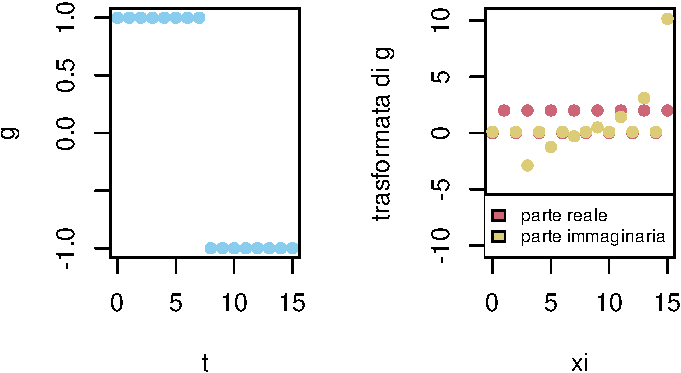
\includegraphics[keepaspectratio]{11-fourier_files/figure-pdf/unnamed-chunk-2-1.pdf}}

}

\caption{esempio di un segnale finito (onda quadra) e della sua
trasformata di Fourier}

\end{figure}%

Possiamo anche verificare la formula di inversione, usando l'opzione
\texttt{inverse\ =TRUE} nella stessa funzione \texttt{fft()}. Bisogna
tuttavia ricordare il fattore \(n\).

\begin{Shaded}
\begin{Highlighting}[]
\NormalTok{g\_ricostruita }\OtherTok{=} \FunctionTok{fft}\NormalTok{(hat\_g, }\AttributeTok{inverse=}\ConstantTok{TRUE}\NormalTok{)}

\CommentTok{\# osserviamo che la ricostruzione coincide con la g ma dilatata di un fattore n}

\FunctionTok{plot}\NormalTok{( t, g\_ricostruita, }\AttributeTok{pch=}\DecValTok{16}\NormalTok{, }\AttributeTok{lwd=}\DecValTok{3}\NormalTok{, }\AttributeTok{col=}\NormalTok{miei\_colori[}\DecValTok{4}\NormalTok{])}
\end{Highlighting}
\end{Shaded}

\begin{center}
\pandocbounded{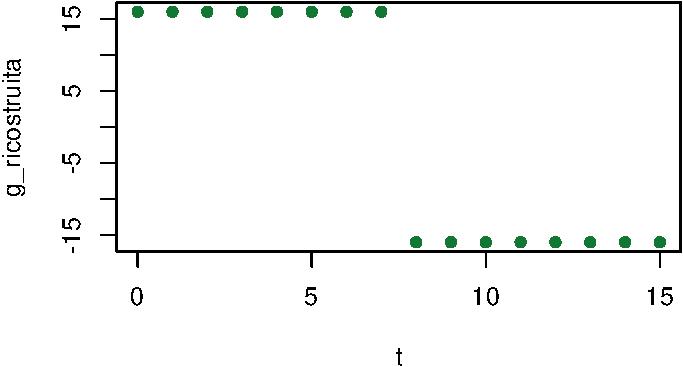
\includegraphics[keepaspectratio]{11-fourier_files/figure-pdf/unnamed-chunk-3-1.pdf}}
\end{center}

Possiamo infine verificare l'identità dell'energia calcolando e
confrontando le norme Euclidee dei vettori:

\begin{Shaded}
\begin{Highlighting}[]
\FunctionTok{sum}\NormalTok{( }\FunctionTok{abs}\NormalTok{(g)}\SpecialCharTok{\^{}}\DecValTok{2}\NormalTok{ ) }
\end{Highlighting}
\end{Shaded}

\begin{verbatim}
[1] 16
\end{verbatim}

\begin{Shaded}
\begin{Highlighting}[]
\FunctionTok{sum}\NormalTok{( }\FunctionTok{abs}\NormalTok{(hat\_g)}\SpecialCharTok{\^{}}\DecValTok{2}\NormalTok{)}
\end{Highlighting}
\end{Shaded}

\begin{verbatim}
[1] 256
\end{verbatim}

\begin{Shaded}
\begin{Highlighting}[]
\CommentTok{\# moltiplicando per n la prima si ottiene la seconda, infatti}

\NormalTok{n}\SpecialCharTok{*} \FunctionTok{sum}\NormalTok{( }\FunctionTok{abs}\NormalTok{(g)}\SpecialCharTok{\^{}}\DecValTok{2}\NormalTok{ )}
\end{Highlighting}
\end{Shaded}

\begin{verbatim}
[1] 256
\end{verbatim}

\end{remark}

\section{Caso discreto}\label{sec-fourier-discreta}

Supponiamo ora di osservare un segnale definito su un tempo infinito
discreto \(g: \mathbb{Z} \to \mathbb{C}\) (è una situazione ideale
ovviamente). L'analoga trasformazione stavolta definisce la trasformata
di Fourier a tempi discreti
\[ \hat{g} : [0,1] \to \mathbb{C}, \quad \xi \mapsto \hat{g}(\xi) := \sum_{t \in \mathbb{Z}} g(t) e^{2 \pi i t \xi},\]
purché la serie converga, ad esempio se
\[ \sum_{t \in \mathbb{Z}} |g(t)| < \infty.\]

\begin{remark}
L'intuizione per passare dal finito al discreto è di cambiare la
variabile frequenza nel caso discreto, ossia di passare da \(\xi\) a
\(\xi/n\), in modo che il dominio sia l'intervallo discreto
\(\cur{0,1/n, 2/n, \ldots, (n-1)/n}\). In questo modo, per
\(n \to \infty\) si ottiene una funzione definita sull'intervallo
continuo di frequenze \([0,1]\). Come nel caso finito, si può utilizzare
la frequenza angolare \(\omega = 2 \pi \xi\) per parametrizzare la
trasformata di Fourier. In questo modo tuttavia appare un fattore
\(1/2\pi\) nella formula di inversione (dovuto al cambio di variabile
nell'integrale).
\end{remark}

Anche senza ricorrere all'intuizione sopra, si può dimostrare l'analogo
discreto della formula di inversione, ossia
\[ g(t) =  \int_0^1 \hat{g}(\xi) e^{2 \pi i t \xi}d \xi,\] e l'identità
dell'energia
\[ \sum_{t \in \mathbb{Z}} |g(t)|^2 =  \int_0^1 |\hat{g}(\xi)|^2 d \xi.\]
Senza entrare nei dettagli, il punto chiave è la relazione di
ortogonalità
\[ \int_0^1 e^{2 \pi i s \xi} e^{-2 \pi i t \xi} d \xi = \begin{cases} 1 & \text{se $s=t$,}
\\
0 & \text{altrimenti,}\end{cases}\] che si dimostra ad esempio
integrando per parti. Le due relazioni sopra seguono ripercorrendo la
dimostrazione del caso finito sfruttando questa ortogonalità.

Nel caso di tempi discreti la trasformata di Fourier è particolarmente
utile perché è un cambio di coordinate che si ``comporta'' bene con le
operazioni di traslazione. Se infatti definiamo l'operatore di
\emph{ritardo} \(L\) (in inglese \emph{lag}), che trasforma \(g\) nel
segnale \[ t \mapsto (Lg)(t) = g(t-1),\] allora
\[ \widehat{ Lg} (\xi) = \sum_{t \in \mathbb{Z}} g(t-1)e^{-2 \pi i t \xi} = e^{-2 \pi i \xi} \hat{g}(\xi).\]
In termini fisici, la traslazione (o ritardo) fa acquisire una fase alla
trasformata.

Il punto è che iterando l'operazione, la fase si accumula: posta
\(L^s g(t) = g(t-s)\), ossia \(L\) applicata \(s\)-volte a \(g\), si ha
\[\widehat{ L^s g}(\xi) = e^{-2 \pi i s \xi } \hat{g}(\xi).\] Una
operazione piuttosto naturale quando si intepreta \(g\) come un segnale
è la \emph{convoluzione} con un ``filtro'' \(f\), ossia una ulteriore
funzione \(f: \mathbb{Z} \to \mathbb{C}\) (con delle caratteristiche
opportune). La definizione di convolution \(g*f\) è data dalla seguente
formula: \[ (g * f) (t ) =  \sum_{s  \in \mathbb{Z}} g(t-s) f(s).\]
Passando alla trasformata di Fourier, possiamo scrivere
\[ \begin{split} \widehat{g * f}(\xi) & = \widehat{ \sum_{s  \in \mathbb{Z}} g(\cdot-s) f(s)} (\xi) \\
& = \sum_{s  \in \mathbb{Z}}\widehat{ g(\cdot-s)} (\xi) f(s)\\
&  = \sum_{s  \in \mathbb{Z}} \widehat{ L^s g} (\xi) f(s)\\
& = \sum_{s  \in \mathbb{Z}} e^{-2\pi i s} \hat g (\xi) f(s)\\
& = \hat g (\xi) \sum_{s  \in \mathbb{Z}} e^{-2\pi i s} \hat g (\xi) f(s) = \hat{g}(\xi) \hat{f}(\xi).\end{split}\]
In altri termini, nelle coordinate date dalla trasformata di Fourier (la
base delle frequenze) la convoluzione con un filtro \(f\) si riduce al
prodotto con la sua trasformata di fourier \(\hat{f}\).

In particolare, dall'identità dell'energia segue che
\[ \sum_{ t \in \mathbb{Z}} |g * f|^2(t) = \int_0^1 |\hat{g}|^2(\xi)|\hat{f}|^2(\xi ) d \xi.\]

\section{Caso continuo}\label{sec-fourier-continua}

Accenniamo infine al caso continuo, che corrisponde ad un passaggio al
limite in cui i tempi \(t \in \mathbb{Z}\) sono pensati come
equidistanziati di passo \(\Delta t \to 0\). Ne segue che per descrivere
\(g\) sono necessarie frequenze in intervalli via via più ampi e nel
limite la trasformata di Fourier di \[g : \R \to \mathbb{C}\] è definita
come
\[ \hat{g}: \R \to \mathbb{C}, \quad \hat{g}(\xi) := \int_{-\infty}^\infty g(t) e^{-2\pi i t \xi} d t,\]
purché l'integrale converga, ad esempio se
\[ \int_{-\infty}^\infty |g(t)| d t < \infty.\] Anche in questo caso (ma
è meno immediato) si può mostrare una formula di inversione
\[ g(t) =  \int_{-\infty}^\infty \hat{g}(\xi) e^{2 \pi i t \xi}d \xi,\]
(purché l'integrale abbia senso) e l'identità dell'energia
\[ \int_{-\infty}^\infty |g(t)|^2 d t=  \int_{-\infty}^{\infty} |\hat{g}(\xi)|^2 d \xi.\]
Anche nel caso continuo si può introdurre la convoluzione con un filtro
\(f: \R \to \mathbb{C}\),
\[ g  * f(t) = \int_{-\infty}^\infty g(t-s)f(s) d s,\] e nella base
delle frequenze l'operazione si riduce ad un prodotto:
\[ \widehat{ g * f}(\xi) = \hat g (\xi) \hat f (\xi).\]

\begin{remark}
Come nel caso di tempi discreti, si può utilizzare la frequenza angolare
\(\omega = 2 \pi \xi\) come variabile per la trasformata di Fourier.
Questa è in effetti la variabile utilizzata solitamente per la
definizione della funzione caratteristica di una variabile aleatoria,
come descritta nella Sezione Sezione~\ref{sec-caratteristica}.
\end{remark}

\bookmarksetup{startatroot}

\chapter*{Letture consigliate}\label{letture-consigliate}
\addcontentsline{toc}{chapter}{Letture consigliate}

\markboth{Letture consigliate}{Letture consigliate}

Le seguenti letture \textbf{non sono necessarie per il corso} e non
fanno parte del programma d'esame. Sono suggerite a chi desideri
ampliare la propria cultura sulla probabilità, sulla statistica e sul
ragionamento in condizioni di incertezza, attraverso testi accessibili e
ricchi di esempi, prospettive storiche e riflessioni metodologiche.

\begin{itemize}
\item
  \textbf{E. T. Jaynes, \emph{Probability Theory: The Logic of
  Science}.} Un testo originale e influente che presenta la probabilità
  come estensione della logica al ragionamento in presenza di
  informazione incompleta. Pur contenendo parti matematicamente
  impegnative, può essere letto anche selettivamente ed è
  particolarmente interessante per la sua prospettiva concettuale e
  bayesiana.
\item
  \textbf{Nate Silver, \emph{The Signal and the Noise: Why So Many
  Predictions Fail---but Some Don't}.} Una lettura molto accessibile sul
  problema della previsione in ambiti diversi, dalla meteorologia alla
  finanza, dallo sport alla politica. Il libro discute temi centrali
  quali incertezza, calibrazione delle previsioni, overfitting, qualità
  dei dati e aggiornamento delle probabilità alla luce di nuove
  informazioni.
\item
  \textbf{David Spiegelhalter, \emph{The Art of Statistics: Learning
  from Data}.} Un'introduzione moderna e non tecnica al modo in cui la
  statistica permette di estrarre informazione dai dati. Attraverso
  numerosi esempi reali, affronta questioni quali variabilità,
  inferenza, correlazione, regressione, test statistici, comunicazione
  dell'incertezza e interpretazione critica dei risultati.
\item
  \textbf{Judea Pearl e Dana Mackenzie, \emph{The Book of Why: The New
  Science of Cause and Effect}.} Un'introduzione divulgativa al
  ragionamento causale. Il libro mette in evidenza la differenza tra
  osservare associazioni, formulare previsioni e stabilire relazioni di
  causa-effetto, introducendo alcune delle idee fondamentali della
  moderna teoria della causalità.
\item
  \textbf{Persi Diaconis e Brian Skyrms, \emph{Ten Great Ideas About
  Chance}.} Un percorso storico e concettuale attraverso alcune delle
  principali idee che hanno formato la moderna teoria della probabilità.
  Il libro intreccia matematica, filosofia, giochi d'azzardo, statistica
  e teoria della decisione, offrendo una prospettiva ampia sul
  significato e sull'uso del caso nelle scienze.
\end{itemize}


\backmatter


\end{document}
